\documentclass[twoside]{book}

% Packages required by doxygen
\usepackage{fixltx2e}
\usepackage{calc}
\usepackage{doxygen}
\usepackage[export]{adjustbox} % also loads graphicx
\usepackage{graphicx}
\usepackage[utf8]{inputenc}
\usepackage{makeidx}
\usepackage{multicol}
\usepackage{multirow}
\PassOptionsToPackage{warn}{textcomp}
\usepackage{textcomp}
\usepackage[nointegrals]{wasysym}
\usepackage[table]{xcolor}

% Font selection
\usepackage[T1]{fontenc}
\usepackage[scaled=.90]{helvet}
\usepackage{courier}
\usepackage{amssymb}
\usepackage{sectsty}
\renewcommand{\familydefault}{\sfdefault}
\allsectionsfont{%
  \fontseries{bc}\selectfont%
  \color{darkgray}%
}
\renewcommand{\DoxyLabelFont}{%
  \fontseries{bc}\selectfont%
  \color{darkgray}%
}
\newcommand{\+}{\discretionary{\mbox{\scriptsize$\hookleftarrow$}}{}{}}

% Page & text layout
\usepackage{geometry}
\geometry{%
  a4paper,%
  top=2.5cm,%
  bottom=2.5cm,%
  left=2.5cm,%
  right=2.5cm%
}
\tolerance=750
\hfuzz=15pt
\hbadness=750
\setlength{\emergencystretch}{15pt}
\setlength{\parindent}{0cm}
\setlength{\parskip}{3ex plus 2ex minus 2ex}
\makeatletter
\renewcommand{\paragraph}{%
  \@startsection{paragraph}{4}{0ex}{-1.0ex}{1.0ex}{%
    \normalfont\normalsize\bfseries\SS@parafont%
  }%
}
\renewcommand{\subparagraph}{%
  \@startsection{subparagraph}{5}{0ex}{-1.0ex}{1.0ex}{%
    \normalfont\normalsize\bfseries\SS@subparafont%
  }%
}
\makeatother

% Headers & footers
\usepackage{fancyhdr}
\pagestyle{fancyplain}
\fancyhead[LE]{\fancyplain{}{\bfseries\thepage}}
\fancyhead[CE]{\fancyplain{}{}}
\fancyhead[RE]{\fancyplain{}{\bfseries\leftmark}}
\fancyhead[LO]{\fancyplain{}{\bfseries\rightmark}}
\fancyhead[CO]{\fancyplain{}{}}
\fancyhead[RO]{\fancyplain{}{\bfseries\thepage}}
\fancyfoot[LE]{\fancyplain{}{}}
\fancyfoot[CE]{\fancyplain{}{}}
\fancyfoot[RE]{\fancyplain{}{\bfseries\scriptsize Generated by Doxygen }}
\fancyfoot[LO]{\fancyplain{}{\bfseries\scriptsize Generated by Doxygen }}
\fancyfoot[CO]{\fancyplain{}{}}
\fancyfoot[RO]{\fancyplain{}{}}
\renewcommand{\footrulewidth}{0.4pt}
\renewcommand{\chaptermark}[1]{%
  \markboth{#1}{}%
}
\renewcommand{\sectionmark}[1]{%
  \markright{\thesection\ #1}%
}

% Indices & bibliography
\usepackage{natbib}
\usepackage[titles]{tocloft}
\setcounter{tocdepth}{3}
\setcounter{secnumdepth}{5}
\makeindex

% Hyperlinks (required, but should be loaded last)
\usepackage{ifpdf}
\ifpdf
  \usepackage[pdftex,pagebackref=true]{hyperref}
\else
  \usepackage[ps2pdf,pagebackref=true]{hyperref}
\fi
\hypersetup{%
  colorlinks=true,%
  linkcolor=blue,%
  citecolor=blue,%
  unicode%
}

% Custom commands
\newcommand{\clearemptydoublepage}{%
  \newpage{\pagestyle{empty}\cleardoublepage}%
}

\usepackage{caption}
\captionsetup{labelsep=space,justification=centering,font={bf},singlelinecheck=off,skip=4pt,position=top}

%===== C O N T E N T S =====

\begin{document}

% Titlepage & ToC
\hypersetup{pageanchor=false,
             bookmarksnumbered=true,
             pdfencoding=unicode
            }
\pagenumbering{roman}
\begin{titlepage}
\vspace*{7cm}
\begin{center}%
{\Large Ray\+Tracer }\\
\vspace*{1cm}
{\large Generated by Doxygen 1.8.11}\\
\end{center}
\end{titlepage}
\clearemptydoublepage
\tableofcontents
\clearemptydoublepage
\pagenumbering{arabic}
\hypersetup{pageanchor=true}

%--- Begin generated contents ---
\chapter{Namespace Index}
\section{Namespace List}
Here is a list of all namespaces with brief descriptions\+:\begin{DoxyCompactList}
\item\contentsline{section}{\hyperlink{namespacelinalg}{linalg} }{\pageref{namespacelinalg}}{}
\item\contentsline{section}{\hyperlink{namespacesymcpp}{symcpp} }{\pageref{namespacesymcpp}}{}
\item\contentsline{section}{\hyperlink{namespaceutility}{utility} }{\pageref{namespaceutility}}{}
\end{DoxyCompactList}

\chapter{Hierarchical Index}
\section{Class Hierarchy}
This inheritance list is sorted roughly, but not completely, alphabetically\+:\begin{DoxyCompactList}
\item \contentsline{section}{Background}{\pageref{classBackground}}{}
\item \contentsline{section}{Bounding\+Box}{\pageref{classBoundingBox}}{}
\item \contentsline{section}{B\+V\+H\+Construction\+Node}{\pageref{structBVHConstructionNode}}{}
\item \contentsline{section}{B\+V\+H\+Linear\+Node}{\pageref{structBVHLinearNode}}{}
\item \contentsline{section}{camera\+::Camera}{\pageref{classcamera_1_1Camera}}{}
\begin{DoxyCompactList}
\item \contentsline{section}{camera\+::Pin\+Hole\+Camera}{\pageref{classcamera_1_1PinHoleCamera}}{}
\end{DoxyCompactList}
\item \contentsline{section}{symcpp\+::Complex\+Token}{\pageref{structsymcpp_1_1ComplexToken}}{}
\item \contentsline{section}{B\+V\+H\+Construction\+Node\+::Construction\+Children}{\pageref{unionBVHConstructionNode_1_1ConstructionChildren}}{}
\item \contentsline{section}{C\+S\+G\+Component}{\pageref{classCSGComponent}}{}
\begin{DoxyCompactList}
\item \contentsline{section}{C\+S\+G\+Difference}{\pageref{classCSGDifference}}{}
\item \contentsline{section}{C\+S\+G\+Intersection}{\pageref{classCSGIntersection}}{}
\item \contentsline{section}{C\+S\+G\+Leaf}{\pageref{classCSGLeaf}}{}
\item \contentsline{section}{C\+S\+G\+Union}{\pageref{classCSGUnion}}{}
\end{DoxyCompactList}
\item \contentsline{section}{symcpp\+::Expression}{\pageref{classsymcpp_1_1Expression}}{}
\begin{DoxyCompactList}
\item \contentsline{section}{symcpp\+::Add}{\pageref{classsymcpp_1_1Add}}{}
\item \contentsline{section}{symcpp\+::Constant}{\pageref{classsymcpp_1_1Constant}}{}
\item \contentsline{section}{symcpp\+::Divide}{\pageref{classsymcpp_1_1Divide}}{}
\item \contentsline{section}{symcpp\+::Multiply}{\pageref{classsymcpp_1_1Multiply}}{}
\item \contentsline{section}{symcpp\+::Power}{\pageref{classsymcpp_1_1Power}}{}
\item \contentsline{section}{symcpp\+::Subtract}{\pageref{classsymcpp_1_1Subtract}}{}
\item \contentsline{section}{symcpp\+::Unary\+Operator}{\pageref{classsymcpp_1_1UnaryOperator}}{}
\begin{DoxyCompactList}
\item \contentsline{section}{symcpp\+::Cosine}{\pageref{classsymcpp_1_1Cosine}}{}
\item \contentsline{section}{symcpp\+::Exponential}{\pageref{classsymcpp_1_1Exponential}}{}
\item \contentsline{section}{symcpp\+::Logarithm}{\pageref{classsymcpp_1_1Logarithm}}{}
\item \contentsline{section}{symcpp\+::Sine}{\pageref{classsymcpp_1_1Sine}}{}
\end{DoxyCompactList}
\item \contentsline{section}{symcpp\+::Variable}{\pageref{classsymcpp_1_1Variable}}{}
\end{DoxyCompactList}
\item \contentsline{section}{Face\+Data}{\pageref{structFaceData}}{}
\item \contentsline{section}{Fixed\+Size\+Stack$<$ V, N $>$}{\pageref{classFixedSizeStack}}{}
\item \contentsline{section}{Intersection}{\pageref{classIntersection}}{}
\item \contentsline{section}{Intersection\+Properties}{\pageref{classIntersectionProperties}}{}
\item \contentsline{section}{Interval}{\pageref{classInterval}}{}
\item \contentsline{section}{Light}{\pageref{classLight}}{}
\begin{DoxyCompactList}
\item \contentsline{section}{Distant\+Point\+Source}{\pageref{classDistantPointSource}}{}
\item \contentsline{section}{Point\+Source}{\pageref{classPointSource}}{}
\item \contentsline{section}{Random\+Light}{\pageref{classRandomLight}}{}
\item \contentsline{section}{Spot\+Light}{\pageref{classSpotLight}}{}
\end{DoxyCompactList}
\item \contentsline{section}{B\+V\+H\+Linear\+Node\+::Linear\+Second\+Child}{\pageref{unionBVHLinearNode_1_1LinearSecondChild}}{}
\item \contentsline{section}{Material}{\pageref{classMaterial}}{}
\item \contentsline{section}{linalg\+::Matrix3D}{\pageref{classlinalg_1_1Matrix3D}}{}
\item \contentsline{section}{M\+T\+L\+Lib}{\pageref{classMTLLib}}{}
\item \contentsline{section}{O\+B\+J\+File}{\pageref{classOBJFile}}{}
\item \contentsline{section}{utility\+::Quadratic\+Solution}{\pageref{structutility_1_1QuadraticSolution}}{}
\item \contentsline{section}{Ray}{\pageref{classRay}}{}
\item \contentsline{section}{Render\+Object}{\pageref{classRenderObject}}{}
\begin{DoxyCompactList}
\item \contentsline{section}{Bounded\+Volume}{\pageref{classBoundedVolume}}{}
\begin{DoxyCompactList}
\item \contentsline{section}{Binary\+Volume\+Hierarchy}{\pageref{classBinaryVolumeHierarchy}}{}
\item \contentsline{section}{Implicit\+Surface}{\pageref{classImplicitSurface}}{}
\item \contentsline{section}{S\+D\+F\+Object}{\pageref{classSDFObject}}{}
\begin{DoxyCompactList}
\item \contentsline{section}{C\+SG}{\pageref{classCSG}}{}
\item \contentsline{section}{S\+D\+F\+Box}{\pageref{classSDFBox}}{}
\item \contentsline{section}{S\+D\+F\+Cylinder}{\pageref{classSDFCylinder}}{}
\item \contentsline{section}{S\+D\+F\+Sphere}{\pageref{classSDFSphere}}{}
\end{DoxyCompactList}
\item \contentsline{section}{Simple\+Sphere}{\pageref{classSimpleSphere}}{}
\item \contentsline{section}{Triangle}{\pageref{classTriangle}}{}
\end{DoxyCompactList}
\item \contentsline{section}{Simple\+Plane}{\pageref{classSimplePlane}}{}
\end{DoxyCompactList}
\item \contentsline{section}{Scene}{\pageref{classScene}}{}
\item \contentsline{section}{symcpp\+::Symbolic\+Graph}{\pageref{classsymcpp_1_1SymbolicGraph}}{}
\item \contentsline{section}{linalg\+::Transformation}{\pageref{classlinalg_1_1Transformation}}{}
\item \contentsline{section}{U\+V\+Map$<$ S, T $>$}{\pageref{classUVMap}}{}
\item \contentsline{section}{U\+V\+Map$<$ Vector3D, T $>$}{\pageref{classUVMap}}{}
\begin{DoxyCompactList}
\item \contentsline{section}{Sphere\+Map$<$ T $>$}{\pageref{classSphereMap}}{}
\end{DoxyCompactList}
\item \contentsline{section}{U\+V\+Map$<$ Vector3D, Vector3D $>$}{\pageref{classUVMap}}{}
\begin{DoxyCompactList}
\item \contentsline{section}{Sphere\+Map$<$ Vector3D $>$}{\pageref{classSphereMap}}{}
\end{DoxyCompactList}
\item \contentsline{section}{Vector3D}{\pageref{classVector3D}}{}
\end{DoxyCompactList}

\chapter{Class Index}
\section{Class List}
Here are the classes, structs, unions and interfaces with brief descriptions\+:\begin{DoxyCompactList}
\item\contentsline{section}{\mbox{\hyperlink{classsymcpp_1_1Add}{symcpp\+::\+Add}} }{\pageref{classsymcpp_1_1Add}}{}
\item\contentsline{section}{\mbox{\hyperlink{classBackground}{Background}} }{\pageref{classBackground}}{}
\item\contentsline{section}{\mbox{\hyperlink{classBinaryVolumeHierarchy}{Binary\+Volume\+Hierarchy}} \\*Acceleration structure for ensemble of bounded volumes }{\pageref{classBinaryVolumeHierarchy}}{}
\item\contentsline{section}{\mbox{\hyperlink{classBoundedVolume}{Bounded\+Volume}} \\*Abstract class implemented by objects that can be contained in a volume }{\pageref{classBoundedVolume}}{}
\item\contentsline{section}{\mbox{\hyperlink{classBoundingBox}{Bounding\+Box}} \\*A cuboid in 3D space for estimating the position of objects }{\pageref{classBoundingBox}}{}
\item\contentsline{section}{\mbox{\hyperlink{structBVHConstructionNode}{B\+V\+H\+Construction\+Node}} }{\pageref{structBVHConstructionNode}}{}
\item\contentsline{section}{\mbox{\hyperlink{structBVHLinearNode}{B\+V\+H\+Linear\+Node}} }{\pageref{structBVHLinearNode}}{}
\item\contentsline{section}{\mbox{\hyperlink{classcamera_1_1Camera}{camera\+::\+Camera}} }{\pageref{classcamera_1_1Camera}}{}
\item\contentsline{section}{\mbox{\hyperlink{structsymcpp_1_1ComplexToken}{symcpp\+::\+Complex\+Token}} }{\pageref{structsymcpp_1_1ComplexToken}}{}
\item\contentsline{section}{\mbox{\hyperlink{classsymcpp_1_1Constant}{symcpp\+::\+Constant}} }{\pageref{classsymcpp_1_1Constant}}{}
\item\contentsline{section}{\mbox{\hyperlink{unionBVHConstructionNode_1_1ConstructionChildren}{B\+V\+H\+Construction\+Node\+::\+Construction\+Children}} }{\pageref{unionBVHConstructionNode_1_1ConstructionChildren}}{}
\item\contentsline{section}{\mbox{\hyperlink{classsymcpp_1_1Cosine}{symcpp\+::\+Cosine}} }{\pageref{classsymcpp_1_1Cosine}}{}
\item\contentsline{section}{\mbox{\hyperlink{classCSG}{C\+SG}} \\*This renderable object represents a constructive solid geometry }{\pageref{classCSG}}{}
\item\contentsline{section}{\mbox{\hyperlink{classCSGComponent}{C\+S\+G\+Component}} \\*Interface for nodes in C\+S\+G-\/\+Tree according to composition-\/pattern }{\pageref{classCSGComponent}}{}
\item\contentsline{section}{\mbox{\hyperlink{classCSGDifference}{C\+S\+G\+Difference}} \\*A difference node in the C\+S\+G-\/\+Tree }{\pageref{classCSGDifference}}{}
\item\contentsline{section}{\mbox{\hyperlink{classCSGIntersection}{C\+S\+G\+Intersection}} \\*An intersection node in the C\+S\+G-\/\+Tree }{\pageref{classCSGIntersection}}{}
\item\contentsline{section}{\mbox{\hyperlink{classCSGLeaf}{C\+S\+G\+Leaf}} \\*Essentially a wrapper for Distance\+Estimated\+Object. They are leafs in the C\+S\+G-\/\+Tree }{\pageref{classCSGLeaf}}{}
\item\contentsline{section}{\mbox{\hyperlink{classCSGUnion}{C\+S\+G\+Union}} \\*A union node in the C\+S\+G-\/\+Tree }{\pageref{classCSGUnion}}{}
\item\contentsline{section}{\mbox{\hyperlink{classDistantPointSource}{Distant\+Point\+Source}} }{\pageref{classDistantPointSource}}{}
\item\contentsline{section}{\mbox{\hyperlink{classsymcpp_1_1Divide}{symcpp\+::\+Divide}} }{\pageref{classsymcpp_1_1Divide}}{}
\item\contentsline{section}{\mbox{\hyperlink{classsymcpp_1_1Exponential}{symcpp\+::\+Exponential}} }{\pageref{classsymcpp_1_1Exponential}}{}
\item\contentsline{section}{\mbox{\hyperlink{classsymcpp_1_1Expression}{symcpp\+::\+Expression}} }{\pageref{classsymcpp_1_1Expression}}{}
\item\contentsline{section}{\mbox{\hyperlink{structFaceData}{Face\+Data}} }{\pageref{structFaceData}}{}
\item\contentsline{section}{\mbox{\hyperlink{classFixedSizeStack}{Fixed\+Size\+Stack$<$ V, N $>$}} \\*A stack that can contain at most N elements. If more are pushed to the stack, it will crash. No error handling is done. If top is called on an empty stack, it will crash }{\pageref{classFixedSizeStack}}{}
\item\contentsline{section}{\mbox{\hyperlink{classImplicitSurface}{Implicit\+Surface}} \\*\mbox{\hyperlink{classRenderObject}{Render\+Object}} for the surface implicitly given by F(x,y,z) = 0 }{\pageref{classImplicitSurface}}{}
\item\contentsline{section}{\mbox{\hyperlink{classIntersection}{Intersection}} \\*Class for storing information about intersection of a \mbox{\hyperlink{classRay}{Ray}} and a \mbox{\hyperlink{classRenderObject}{Render\+Object}} }{\pageref{classIntersection}}{}
\item\contentsline{section}{\mbox{\hyperlink{classIntersectionProperties}{Intersection\+Properties}} \\*Class for storing information about the local properties of a \mbox{\hyperlink{classRenderObject}{Render\+Object}} at a specific point in space }{\pageref{classIntersectionProperties}}{}
\item\contentsline{section}{\mbox{\hyperlink{classInterval}{Interval}} \\*The closed interval \mbox{[}mini, maxi\mbox{]} }{\pageref{classInterval}}{}
\item\contentsline{section}{\mbox{\hyperlink{classLight}{Light}} \\*Abstract class for lights used in \mbox{\hyperlink{classScene}{Scene}} }{\pageref{classLight}}{}
\item\contentsline{section}{\mbox{\hyperlink{unionBVHLinearNode_1_1LinearSecondChild}{B\+V\+H\+Linear\+Node\+::\+Linear\+Second\+Child}} }{\pageref{unionBVHLinearNode_1_1LinearSecondChild}}{}
\item\contentsline{section}{\mbox{\hyperlink{classsymcpp_1_1Logarithm}{symcpp\+::\+Logarithm}} }{\pageref{classsymcpp_1_1Logarithm}}{}
\item\contentsline{section}{\mbox{\hyperlink{classMaterial}{Material}} \\*Typically stores information about material of Render\+Objects }{\pageref{classMaterial}}{}
\item\contentsline{section}{\mbox{\hyperlink{classlinalg_1_1Matrix3D}{linalg\+::\+Matrix3D}} \\*Square 3x3 Matrix }{\pageref{classlinalg_1_1Matrix3D}}{}
\item\contentsline{section}{\mbox{\hyperlink{classMTLLib}{M\+T\+L\+Lib}} \\*Class for loading wavefront .mtl files }{\pageref{classMTLLib}}{}
\item\contentsline{section}{\mbox{\hyperlink{classsymcpp_1_1Multiply}{symcpp\+::\+Multiply}} }{\pageref{classsymcpp_1_1Multiply}}{}
\item\contentsline{section}{\mbox{\hyperlink{classOBJFile}{O\+B\+J\+File}} \\*Class for loading wavefront .obj files }{\pageref{classOBJFile}}{}
\item\contentsline{section}{\mbox{\hyperlink{classcamera_1_1PinHoleCamera}{camera\+::\+Pin\+Hole\+Camera}} \\*Implementation of \mbox{\hyperlink{classcamera_1_1Camera}{Camera}} class }{\pageref{classcamera_1_1PinHoleCamera}}{}
\item\contentsline{section}{\mbox{\hyperlink{classPointSource}{Point\+Source}} \\*A very simple light source consisting of only one point in 3D Space }{\pageref{classPointSource}}{}
\item\contentsline{section}{\mbox{\hyperlink{classsymcpp_1_1Power}{symcpp\+::\+Power}} }{\pageref{classsymcpp_1_1Power}}{}
\item\contentsline{section}{\mbox{\hyperlink{structutility_1_1QuadraticSolution}{utility\+::\+Quadratic\+Solution}} \\*Class containing solution to quadratic equation }{\pageref{structutility_1_1QuadraticSolution}}{}
\item\contentsline{section}{\mbox{\hyperlink{classRandomLight}{Random\+Light}} }{\pageref{classRandomLight}}{}
\item\contentsline{section}{\mbox{\hyperlink{classRay}{Ray}} }{\pageref{classRay}}{}
\item\contentsline{section}{\mbox{\hyperlink{classRenderObject}{Render\+Object}} \\*Abstract class for renderable objects }{\pageref{classRenderObject}}{}
\item\contentsline{section}{\mbox{\hyperlink{classScene}{Scene}} \\*The Scene-\/\+Object is used to compose Render\+Objects, Lights, the \mbox{\hyperlink{classBackground}{Background}} and render them }{\pageref{classScene}}{}
\item\contentsline{section}{\mbox{\hyperlink{classSDFBox}{S\+D\+F\+Box}} }{\pageref{classSDFBox}}{}
\item\contentsline{section}{\mbox{\hyperlink{classSDFCylinder}{S\+D\+F\+Cylinder}} }{\pageref{classSDFCylinder}}{}
\item\contentsline{section}{\mbox{\hyperlink{classSDFObject}{S\+D\+F\+Object}} \\*Interface for an object that can be Sphere-\/\+Marched }{\pageref{classSDFObject}}{}
\item\contentsline{section}{\mbox{\hyperlink{classSDFSphere}{S\+D\+F\+Sphere}} }{\pageref{classSDFSphere}}{}
\item\contentsline{section}{\mbox{\hyperlink{classSimplePlane}{Simple\+Plane}} \\*An infinite plane }{\pageref{classSimplePlane}}{}
\item\contentsline{section}{\mbox{\hyperlink{classSimpleSphere}{Simple\+Sphere}} \\*A simple, uniformly textured sphere, implements \mbox{\hyperlink{classRenderObject}{Render\+Object}} }{\pageref{classSimpleSphere}}{}
\item\contentsline{section}{\mbox{\hyperlink{classsymcpp_1_1Sine}{symcpp\+::\+Sine}} }{\pageref{classsymcpp_1_1Sine}}{}
\item\contentsline{section}{\mbox{\hyperlink{classSphereMap}{Sphere\+Map$<$ T $>$}} }{\pageref{classSphereMap}}{}
\item\contentsline{section}{\mbox{\hyperlink{classSpotLight}{Spot\+Light}} }{\pageref{classSpotLight}}{}
\item\contentsline{section}{\mbox{\hyperlink{classsymcpp_1_1Subtract}{symcpp\+::\+Subtract}} }{\pageref{classsymcpp_1_1Subtract}}{}
\item\contentsline{section}{\mbox{\hyperlink{classsymcpp_1_1SymbolicGraph}{symcpp\+::\+Symbolic\+Graph}} \\*User-\/friendly wrapper for \mbox{\hyperlink{classsymcpp_1_1Expression}{Expression}} }{\pageref{classsymcpp_1_1SymbolicGraph}}{}
\item\contentsline{section}{\mbox{\hyperlink{classlinalg_1_1Transformation}{linalg\+::\+Transformation}} \\*\mbox{\hyperlink{classlinalg_1_1Transformation}{Transformation}} objects represent angle-\/preserving transformations }{\pageref{classlinalg_1_1Transformation}}{}
\item\contentsline{section}{\mbox{\hyperlink{classTriangle}{Triangle}} \\*A \mbox{\hyperlink{classTriangle}{Triangle}} implementing \mbox{\hyperlink{classBoundedVolume}{Bounded\+Volume}}, \mbox{\hyperlink{classRenderObject}{Render\+Object}} }{\pageref{classTriangle}}{}
\item\contentsline{section}{\mbox{\hyperlink{classsymcpp_1_1UnaryOperator}{symcpp\+::\+Unary\+Operator}} }{\pageref{classsymcpp_1_1UnaryOperator}}{}
\item\contentsline{section}{\mbox{\hyperlink{classUVMap}{U\+V\+Map$<$ S, T $>$}} }{\pageref{classUVMap}}{}
\item\contentsline{section}{\mbox{\hyperlink{classsymcpp_1_1Variable}{symcpp\+::\+Variable}} }{\pageref{classsymcpp_1_1Variable}}{}
\item\contentsline{section}{\mbox{\hyperlink{classVector3D}{Vector3D}} \\*Vector in 3D space with usual arithmetics }{\pageref{classVector3D}}{}
\end{DoxyCompactList}

\chapter{File Index}
\section{File List}
Here is a list of all files with brief descriptions\+:\begin{DoxyCompactList}
\item\contentsline{section}{src/\hyperlink{Background_8cpp}{Background.\+cpp} }{\pageref{Background_8cpp}}{}
\item\contentsline{section}{src/\hyperlink{Background_8h}{Background.\+h} }{\pageref{Background_8h}}{}
\item\contentsline{section}{src/\hyperlink{BinaryVolumeHierarchy_8cpp}{Binary\+Volume\+Hierarchy.\+cpp} }{\pageref{BinaryVolumeHierarchy_8cpp}}{}
\item\contentsline{section}{src/\hyperlink{BinaryVolumeHierarchy_8h}{Binary\+Volume\+Hierarchy.\+h} }{\pageref{BinaryVolumeHierarchy_8h}}{}
\item\contentsline{section}{src/\hyperlink{BoundedVolume_8cpp}{Bounded\+Volume.\+cpp} }{\pageref{BoundedVolume_8cpp}}{}
\item\contentsline{section}{src/\hyperlink{BoundedVolume_8h}{Bounded\+Volume.\+h} }{\pageref{BoundedVolume_8h}}{}
\item\contentsline{section}{src/\hyperlink{BoundingBox_8cpp}{Bounding\+Box.\+cpp} }{\pageref{BoundingBox_8cpp}}{}
\item\contentsline{section}{src/\hyperlink{BoundingBox_8h}{Bounding\+Box.\+h} }{\pageref{BoundingBox_8h}}{}
\item\contentsline{section}{src/\hyperlink{Camera_8cpp}{Camera.\+cpp} }{\pageref{Camera_8cpp}}{}
\item\contentsline{section}{src/\hyperlink{Camera_8h}{Camera.\+h} }{\pageref{Camera_8h}}{}
\item\contentsline{section}{src/\hyperlink{DistantPointSource_8cpp}{Distant\+Point\+Source.\+cpp} }{\pageref{DistantPointSource_8cpp}}{}
\item\contentsline{section}{src/\hyperlink{DistantPointSource_8h}{Distant\+Point\+Source.\+h} }{\pageref{DistantPointSource_8h}}{}
\item\contentsline{section}{src/\hyperlink{ImplicitSurface_8cpp}{Implicit\+Surface.\+cpp} }{\pageref{ImplicitSurface_8cpp}}{}
\item\contentsline{section}{src/\hyperlink{ImplicitSurface_8h}{Implicit\+Surface.\+h} }{\pageref{ImplicitSurface_8h}}{}
\item\contentsline{section}{src/\hyperlink{Intersection_8cpp}{Intersection.\+cpp} }{\pageref{Intersection_8cpp}}{}
\item\contentsline{section}{src/\hyperlink{Intersection_8h}{Intersection.\+h} }{\pageref{Intersection_8h}}{}
\item\contentsline{section}{src/\hyperlink{IntersectionProperties_8cpp}{Intersection\+Properties.\+cpp} }{\pageref{IntersectionProperties_8cpp}}{}
\item\contentsline{section}{src/\hyperlink{IntersectionProperties_8h}{Intersection\+Properties.\+h} }{\pageref{IntersectionProperties_8h}}{}
\item\contentsline{section}{src/\hyperlink{Interval_8cpp}{Interval.\+cpp} }{\pageref{Interval_8cpp}}{}
\item\contentsline{section}{src/\hyperlink{Interval_8h}{Interval.\+h} }{\pageref{Interval_8h}}{}
\item\contentsline{section}{src/\hyperlink{Light_8cpp}{Light.\+cpp} }{\pageref{Light_8cpp}}{}
\item\contentsline{section}{src/\hyperlink{Light_8h}{Light.\+h} }{\pageref{Light_8h}}{}
\item\contentsline{section}{src/\hyperlink{main_8cpp}{main.\+cpp} }{\pageref{main_8cpp}}{}
\item\contentsline{section}{src/\hyperlink{Material_8cpp}{Material.\+cpp} }{\pageref{Material_8cpp}}{}
\item\contentsline{section}{src/\hyperlink{Material_8h}{Material.\+h} }{\pageref{Material_8h}}{}
\item\contentsline{section}{src/\hyperlink{MTLLib_8cpp}{M\+T\+L\+Lib.\+cpp} }{\pageref{MTLLib_8cpp}}{}
\item\contentsline{section}{src/\hyperlink{MTLLib_8h}{M\+T\+L\+Lib.\+h} }{\pageref{MTLLib_8h}}{}
\item\contentsline{section}{src/\hyperlink{OBJFile_8cpp}{O\+B\+J\+File.\+cpp} }{\pageref{OBJFile_8cpp}}{}
\item\contentsline{section}{src/\hyperlink{OBJFile_8h}{O\+B\+J\+File.\+h} }{\pageref{OBJFile_8h}}{}
\item\contentsline{section}{src/\hyperlink{PinHoleCamera_8cpp}{Pin\+Hole\+Camera.\+cpp} }{\pageref{PinHoleCamera_8cpp}}{}
\item\contentsline{section}{src/\hyperlink{PinHoleCamera_8h}{Pin\+Hole\+Camera.\+h} }{\pageref{PinHoleCamera_8h}}{}
\item\contentsline{section}{src/\hyperlink{PointSource_8cpp}{Point\+Source.\+cpp} }{\pageref{PointSource_8cpp}}{}
\item\contentsline{section}{src/\hyperlink{PointSource_8h}{Point\+Source.\+h} }{\pageref{PointSource_8h}}{}
\item\contentsline{section}{src/\hyperlink{RandomLight_8cpp}{Random\+Light.\+cpp} }{\pageref{RandomLight_8cpp}}{}
\item\contentsline{section}{src/\hyperlink{RandomLight_8h}{Random\+Light.\+h} }{\pageref{RandomLight_8h}}{}
\item\contentsline{section}{src/\hyperlink{Ray_8cpp}{Ray.\+cpp} }{\pageref{Ray_8cpp}}{}
\item\contentsline{section}{src/\hyperlink{Ray_8h}{Ray.\+h} }{\pageref{Ray_8h}}{}
\item\contentsline{section}{src/\hyperlink{RenderObject_8cpp}{Render\+Object.\+cpp} }{\pageref{RenderObject_8cpp}}{}
\item\contentsline{section}{src/\hyperlink{RenderObject_8h}{Render\+Object.\+h} }{\pageref{RenderObject_8h}}{}
\item\contentsline{section}{src/\hyperlink{Scene_8cpp}{Scene.\+cpp} }{\pageref{Scene_8cpp}}{}
\item\contentsline{section}{src/\hyperlink{Scene_8h}{Scene.\+h} }{\pageref{Scene_8h}}{}
\item\contentsline{section}{src/\hyperlink{SimplePlane_8cpp}{Simple\+Plane.\+cpp} }{\pageref{SimplePlane_8cpp}}{}
\item\contentsline{section}{src/\hyperlink{SimplePlane_8h}{Simple\+Plane.\+h} }{\pageref{SimplePlane_8h}}{}
\item\contentsline{section}{src/\hyperlink{SimpleSphere_8cpp}{Simple\+Sphere.\+cpp} }{\pageref{SimpleSphere_8cpp}}{}
\item\contentsline{section}{src/\hyperlink{SimpleSphere_8h}{Simple\+Sphere.\+h} }{\pageref{SimpleSphere_8h}}{}
\item\contentsline{section}{src/\hyperlink{SphereMap_8cpp}{Sphere\+Map.\+cpp} }{\pageref{SphereMap_8cpp}}{}
\item\contentsline{section}{src/\hyperlink{SphereMap_8h}{Sphere\+Map.\+h} }{\pageref{SphereMap_8h}}{}
\item\contentsline{section}{src/\hyperlink{SpotLight_8cpp}{Spot\+Light.\+cpp} }{\pageref{SpotLight_8cpp}}{}
\item\contentsline{section}{src/\hyperlink{SpotLight_8h}{Spot\+Light.\+h} }{\pageref{SpotLight_8h}}{}
\item\contentsline{section}{src/\hyperlink{Triangle_8cpp}{Triangle.\+cpp} }{\pageref{Triangle_8cpp}}{}
\item\contentsline{section}{src/\hyperlink{Triangle_8h}{Triangle.\+h} }{\pageref{Triangle_8h}}{}
\item\contentsline{section}{src/\hyperlink{Utilities_8cpp}{Utilities.\+cpp} }{\pageref{Utilities_8cpp}}{}
\item\contentsline{section}{src/\hyperlink{Utilities_8h}{Utilities.\+h} }{\pageref{Utilities_8h}}{}
\item\contentsline{section}{src/\hyperlink{UVMap_8cpp}{U\+V\+Map.\+cpp} }{\pageref{UVMap_8cpp}}{}
\item\contentsline{section}{src/\hyperlink{UVMap_8h}{U\+V\+Map.\+h} }{\pageref{UVMap_8h}}{}
\item\contentsline{section}{src/\hyperlink{Vector3D_8cpp}{Vector3\+D.\+cpp} }{\pageref{Vector3D_8cpp}}{}
\item\contentsline{section}{src/\hyperlink{Vector3D_8h}{Vector3\+D.\+h} }{\pageref{Vector3D_8h}}{}
\item\contentsline{section}{src/image/\hyperlink{post__process_8cpp}{post\+\_\+process.\+cpp} }{\pageref{post__process_8cpp}}{}
\item\contentsline{section}{src/image/\hyperlink{post__process_8h}{post\+\_\+process.\+h} }{\pageref{post__process_8h}}{}
\item\contentsline{section}{src/linalg/\hyperlink{Matrix3D_8cpp}{Matrix3\+D.\+cpp} }{\pageref{Matrix3D_8cpp}}{}
\item\contentsline{section}{src/linalg/\hyperlink{Matrix3D_8h}{Matrix3\+D.\+h} }{\pageref{Matrix3D_8h}}{}
\item\contentsline{section}{src/linalg/\hyperlink{Transformation_8cpp}{Transformation.\+cpp} }{\pageref{Transformation_8cpp}}{}
\item\contentsline{section}{src/linalg/\hyperlink{Transformation_8h}{Transformation.\+h} }{\pageref{Transformation_8h}}{}
\item\contentsline{section}{src/symcpp/\hyperlink{Add_8cpp}{Add.\+cpp} }{\pageref{Add_8cpp}}{}
\item\contentsline{section}{src/symcpp/\hyperlink{Add_8h}{Add.\+h} }{\pageref{Add_8h}}{}
\item\contentsline{section}{src/symcpp/\hyperlink{Constant_8cpp}{Constant.\+cpp} }{\pageref{Constant_8cpp}}{}
\item\contentsline{section}{src/symcpp/\hyperlink{Constant_8h}{Constant.\+h} }{\pageref{Constant_8h}}{}
\item\contentsline{section}{src/symcpp/\hyperlink{Cosine_8cpp}{Cosine.\+cpp} }{\pageref{Cosine_8cpp}}{}
\item\contentsline{section}{src/symcpp/\hyperlink{Cosine_8h}{Cosine.\+h} }{\pageref{Cosine_8h}}{}
\item\contentsline{section}{src/symcpp/\hyperlink{Divide_8cpp}{Divide.\+cpp} }{\pageref{Divide_8cpp}}{}
\item\contentsline{section}{src/symcpp/\hyperlink{Divide_8h}{Divide.\+h} }{\pageref{Divide_8h}}{}
\item\contentsline{section}{src/symcpp/\hyperlink{Exponential_8cpp}{Exponential.\+cpp} }{\pageref{Exponential_8cpp}}{}
\item\contentsline{section}{src/symcpp/\hyperlink{Exponential_8h}{Exponential.\+h} }{\pageref{Exponential_8h}}{}
\item\contentsline{section}{src/symcpp/\hyperlink{Expression_8cpp}{Expression.\+cpp} }{\pageref{Expression_8cpp}}{}
\item\contentsline{section}{src/symcpp/\hyperlink{Expression_8h}{Expression.\+h} }{\pageref{Expression_8h}}{}
\item\contentsline{section}{src/symcpp/\hyperlink{Logarithm_8cpp}{Logarithm.\+cpp} }{\pageref{Logarithm_8cpp}}{}
\item\contentsline{section}{src/symcpp/\hyperlink{Logarithm_8h}{Logarithm.\+h} }{\pageref{Logarithm_8h}}{}
\item\contentsline{section}{src/symcpp/\hyperlink{Multiply_8cpp}{Multiply.\+cpp} }{\pageref{Multiply_8cpp}}{}
\item\contentsline{section}{src/symcpp/\hyperlink{Multiply_8h}{Multiply.\+h} }{\pageref{Multiply_8h}}{}
\item\contentsline{section}{src/symcpp/\hyperlink{Power_8cpp}{Power.\+cpp} }{\pageref{Power_8cpp}}{}
\item\contentsline{section}{src/symcpp/\hyperlink{Power_8h}{Power.\+h} }{\pageref{Power_8h}}{}
\item\contentsline{section}{src/symcpp/\hyperlink{Sine_8cpp}{Sine.\+cpp} }{\pageref{Sine_8cpp}}{}
\item\contentsline{section}{src/symcpp/\hyperlink{Sine_8h}{Sine.\+h} }{\pageref{Sine_8h}}{}
\item\contentsline{section}{src/symcpp/\hyperlink{Subtract_8cpp}{Subtract.\+cpp} }{\pageref{Subtract_8cpp}}{}
\item\contentsline{section}{src/symcpp/\hyperlink{Subtract_8h}{Subtract.\+h} }{\pageref{Subtract_8h}}{}
\item\contentsline{section}{src/symcpp/\hyperlink{SymbolicGraph_8cpp}{Symbolic\+Graph.\+cpp} }{\pageref{SymbolicGraph_8cpp}}{}
\item\contentsline{section}{src/symcpp/\hyperlink{SymbolicGraph_8h}{Symbolic\+Graph.\+h} }{\pageref{SymbolicGraph_8h}}{}
\item\contentsline{section}{src/symcpp/\hyperlink{UnaryOperator_8cpp}{Unary\+Operator.\+cpp} }{\pageref{UnaryOperator_8cpp}}{}
\item\contentsline{section}{src/symcpp/\hyperlink{UnaryOperator_8h}{Unary\+Operator.\+h} }{\pageref{UnaryOperator_8h}}{}
\item\contentsline{section}{src/symcpp/\hyperlink{Variable_8cpp}{Variable.\+cpp} }{\pageref{Variable_8cpp}}{}
\item\contentsline{section}{src/symcpp/\hyperlink{Variable_8h}{Variable.\+h} }{\pageref{Variable_8h}}{}
\end{DoxyCompactList}

\chapter{Namespace Documentation}
\hypertarget{namespacecamera}{}\section{camera Namespace Reference}
\label{namespacecamera}\index{camera@{camera}}
\subsection*{Classes}
\begin{DoxyCompactItemize}
\item 
class \hyperlink{classcamera_1_1Camera}{Camera}
\item 
class \hyperlink{classcamera_1_1PinHoleCamera}{Pin\+Hole\+Camera}
\begin{DoxyCompactList}\small\item\em Implementation of \hyperlink{classcamera_1_1Camera}{Camera} class. \end{DoxyCompactList}\end{DoxyCompactItemize}
\subsection*{Typedefs}
\begin{DoxyCompactItemize}
\item 
using \hyperlink{namespacecamera_a67b7fb3d5582463a057ed122bf739b7d}{Image} = std\+::vector$<$ std\+::vector$<$ \hyperlink{classVector3D}{Vector3D} $>$$>$
\end{DoxyCompactItemize}


\subsection{Typedef Documentation}
\index{camera@{camera}!Image@{Image}}
\index{Image@{Image}!camera@{camera}}
\subsubsection[{\texorpdfstring{Image}{Image}}]{\setlength{\rightskip}{0pt plus 5cm}using {\bf camera\+::\+Image} = typedef std\+::vector$<$std\+::vector$<${\bf Vector3D}$>$$>$}\hypertarget{namespacecamera_a67b7fb3d5582463a057ed122bf739b7d}{}\label{namespacecamera_a67b7fb3d5582463a057ed122bf739b7d}

\hypertarget{namespaceimage}{}\section{image Namespace Reference}
\label{namespaceimage}\index{image@{image}}
\subsection*{Typedefs}
\begin{DoxyCompactItemize}
\item 
using \mbox{\hyperlink{namespaceimage_af3f0dcb372dbc1b38ba87aae9e2c780c}{Image}} = std\+::vector$<$ std\+::vector$<$ \mbox{\hyperlink{classVector3D}{Vector3D}} $>$ $>$
\end{DoxyCompactItemize}
\subsection*{Functions}
\begin{DoxyCompactItemize}
\item 
\mbox{\hyperlink{namespaceimage_af3f0dcb372dbc1b38ba87aae9e2c780c}{Image}} \mbox{\hyperlink{namespaceimage_a350994eafb0492e40cb74c116873a7ae}{gamma\+\_\+correct}} (const \mbox{\hyperlink{namespaceimage_af3f0dcb372dbc1b38ba87aae9e2c780c}{Image}} \&original, double gamma, double A)
\begin{DoxyCompactList}\small\item\em Apply gamma correction to original. \end{DoxyCompactList}\item 
\mbox{\hyperlink{namespaceimage_af3f0dcb372dbc1b38ba87aae9e2c780c}{Image}} \mbox{\hyperlink{namespaceimage_a0d356b98f4bd21ca658d5c83e191cbe2}{gamma\+\_\+correct}} (const \mbox{\hyperlink{namespaceimage_af3f0dcb372dbc1b38ba87aae9e2c780c}{Image}} \&original, double gamma)
\item 
\mbox{\hyperlink{namespaceimage_af3f0dcb372dbc1b38ba87aae9e2c780c}{Image}} \mbox{\hyperlink{namespaceimage_a3646524ebdcbde53e3d2f4bfa47a024a}{max\+\_\+tone\+\_\+mapping}} (const \mbox{\hyperlink{namespaceimage_af3f0dcb372dbc1b38ba87aae9e2c780c}{Image}} \&original, double max)
\item 
\mbox{\hyperlink{namespaceimage_af3f0dcb372dbc1b38ba87aae9e2c780c}{Image}} \mbox{\hyperlink{namespaceimage_acad5a9459043f5ce5b565e771b0867f8}{max\+\_\+tone\+\_\+mapping}} (const \mbox{\hyperlink{namespaceimage_af3f0dcb372dbc1b38ba87aae9e2c780c}{Image}} \&original)
\item 
\mbox{\hyperlink{namespaceimage_af3f0dcb372dbc1b38ba87aae9e2c780c}{Image}} \mbox{\hyperlink{namespaceimage_ae465266083a6ee29947db193e0881ff2}{anti\+\_\+alias}} (const \mbox{\hyperlink{namespaceimage_af3f0dcb372dbc1b38ba87aae9e2c780c}{Image}} \&original, unsigned int window\+\_\+size)
\end{DoxyCompactItemize}


\subsection{Typedef Documentation}
\mbox{\Hypertarget{namespaceimage_af3f0dcb372dbc1b38ba87aae9e2c780c}\label{namespaceimage_af3f0dcb372dbc1b38ba87aae9e2c780c}} 
\index{image@{image}!Image@{Image}}
\index{Image@{Image}!image@{image}}
\subsubsection{\texorpdfstring{Image}{Image}}
{\footnotesize\ttfamily using \mbox{\hyperlink{namespaceimage_af3f0dcb372dbc1b38ba87aae9e2c780c}{image\+::\+Image}} = typedef std\+::vector$<$std\+::vector$<$\mbox{\hyperlink{classVector3D}{Vector3D}}$>$ $>$}



\subsection{Function Documentation}
\mbox{\Hypertarget{namespaceimage_ae465266083a6ee29947db193e0881ff2}\label{namespaceimage_ae465266083a6ee29947db193e0881ff2}} 
\index{image@{image}!anti\_alias@{anti\_alias}}
\index{anti\_alias@{anti\_alias}!image@{image}}
\subsubsection{\texorpdfstring{anti\_alias()}{anti\_alias()}}
{\footnotesize\ttfamily \mbox{\hyperlink{namespaceimage_af3f0dcb372dbc1b38ba87aae9e2c780c}{Image}} image\+::anti\+\_\+alias (\begin{DoxyParamCaption}\item[{const \mbox{\hyperlink{namespaceimage_af3f0dcb372dbc1b38ba87aae9e2c780c}{Image}} \&}]{original,  }\item[{unsigned int}]{window\+\_\+size }\end{DoxyParamCaption})}

\mbox{\Hypertarget{namespaceimage_a350994eafb0492e40cb74c116873a7ae}\label{namespaceimage_a350994eafb0492e40cb74c116873a7ae}} 
\index{image@{image}!gamma\_correct@{gamma\_correct}}
\index{gamma\_correct@{gamma\_correct}!image@{image}}
\subsubsection{\texorpdfstring{gamma\_correct()}{gamma\_correct()}\hspace{0.1cm}{\footnotesize\ttfamily [1/2]}}
{\footnotesize\ttfamily \mbox{\hyperlink{namespaceimage_af3f0dcb372dbc1b38ba87aae9e2c780c}{Image}} image\+::gamma\+\_\+correct (\begin{DoxyParamCaption}\item[{const \mbox{\hyperlink{namespaceimage_af3f0dcb372dbc1b38ba87aae9e2c780c}{Image}} \&}]{original,  }\item[{double}]{gamma,  }\item[{double}]{A }\end{DoxyParamCaption})}



Apply gamma correction to original. 


\begin{DoxyParams}{Parameters}
{\em original} & The origina image \\
\hline
{\em gamma} & The gamma value \\
\hline
\end{DoxyParams}
\begin{DoxyReturn}{Returns}
Gamma corrected image 
\end{DoxyReturn}
\mbox{\Hypertarget{namespaceimage_a0d356b98f4bd21ca658d5c83e191cbe2}\label{namespaceimage_a0d356b98f4bd21ca658d5c83e191cbe2}} 
\index{image@{image}!gamma\_correct@{gamma\_correct}}
\index{gamma\_correct@{gamma\_correct}!image@{image}}
\subsubsection{\texorpdfstring{gamma\_correct()}{gamma\_correct()}\hspace{0.1cm}{\footnotesize\ttfamily [2/2]}}
{\footnotesize\ttfamily \mbox{\hyperlink{namespaceimage_af3f0dcb372dbc1b38ba87aae9e2c780c}{Image}} image\+::gamma\+\_\+correct (\begin{DoxyParamCaption}\item[{const \mbox{\hyperlink{namespaceimage_af3f0dcb372dbc1b38ba87aae9e2c780c}{Image}} \&}]{original,  }\item[{double}]{gamma }\end{DoxyParamCaption})}

\mbox{\Hypertarget{namespaceimage_a3646524ebdcbde53e3d2f4bfa47a024a}\label{namespaceimage_a3646524ebdcbde53e3d2f4bfa47a024a}} 
\index{image@{image}!max\_tone\_mapping@{max\_tone\_mapping}}
\index{max\_tone\_mapping@{max\_tone\_mapping}!image@{image}}
\subsubsection{\texorpdfstring{max\_tone\_mapping()}{max\_tone\_mapping()}\hspace{0.1cm}{\footnotesize\ttfamily [1/2]}}
{\footnotesize\ttfamily \mbox{\hyperlink{namespaceimage_af3f0dcb372dbc1b38ba87aae9e2c780c}{Image}} image\+::max\+\_\+tone\+\_\+mapping (\begin{DoxyParamCaption}\item[{const \mbox{\hyperlink{namespaceimage_af3f0dcb372dbc1b38ba87aae9e2c780c}{Image}} \&}]{original,  }\item[{double}]{max }\end{DoxyParamCaption})}

\mbox{\Hypertarget{namespaceimage_acad5a9459043f5ce5b565e771b0867f8}\label{namespaceimage_acad5a9459043f5ce5b565e771b0867f8}} 
\index{image@{image}!max\_tone\_mapping@{max\_tone\_mapping}}
\index{max\_tone\_mapping@{max\_tone\_mapping}!image@{image}}
\subsubsection{\texorpdfstring{max\_tone\_mapping()}{max\_tone\_mapping()}\hspace{0.1cm}{\footnotesize\ttfamily [2/2]}}
{\footnotesize\ttfamily \mbox{\hyperlink{namespaceimage_af3f0dcb372dbc1b38ba87aae9e2c780c}{Image}} image\+::max\+\_\+tone\+\_\+mapping (\begin{DoxyParamCaption}\item[{const \mbox{\hyperlink{namespaceimage_af3f0dcb372dbc1b38ba87aae9e2c780c}{Image}} \&}]{original }\end{DoxyParamCaption})}


\hypertarget{namespacelinalg}{}\section{linalg Namespace Reference}
\label{namespacelinalg}\index{linalg@{linalg}}
\subsection*{Classes}
\begin{DoxyCompactItemize}
\item 
class \hyperlink{classlinalg_1_1Matrix3D}{Matrix3D}
\begin{DoxyCompactList}\small\item\em Square 3x3 Matrix. \end{DoxyCompactList}\item 
class \hyperlink{classlinalg_1_1Transformation}{Transformation}
\begin{DoxyCompactList}\small\item\em \hyperlink{classlinalg_1_1Transformation}{Transformation} objects represent angle-\/preserving transformations. \end{DoxyCompactList}\end{DoxyCompactItemize}
\subsection*{Functions}
\begin{DoxyCompactItemize}
\item 
\hyperlink{classVector3D}{Vector3D} \hyperlink{namespacelinalg_a64ac8620c880fd85e0163941dbd2ce92}{operator$\ast$} (const \hyperlink{classlinalg_1_1Matrix3D}{Matrix3D} \&A, const \hyperlink{classVector3D}{Vector3D} \&v)
\item 
\hyperlink{classlinalg_1_1Matrix3D}{Matrix3D} \hyperlink{namespacelinalg_a6bacae184309d12c829d272de83d0534}{operator$\ast$} (\hyperlink{classlinalg_1_1Matrix3D}{Matrix3D} A, const \hyperlink{classlinalg_1_1Matrix3D}{Matrix3D} \&B)
\item 
\hyperlink{classlinalg_1_1Matrix3D}{Matrix3D} \hyperlink{namespacelinalg_a556fef68037fa24314207620fa918536}{operator+} (\hyperlink{classlinalg_1_1Matrix3D}{Matrix3D} A, const \hyperlink{classlinalg_1_1Matrix3D}{Matrix3D} \&B)
\end{DoxyCompactItemize}


\subsection{Function Documentation}
\index{linalg@{linalg}!operator$\ast$@{operator$\ast$}}
\index{operator$\ast$@{operator$\ast$}!linalg@{linalg}}
\subsubsection[{\texorpdfstring{operator$\ast$(const Matrix3\+D \&\+A, const Vector3\+D \&v)}{operator*(const Matrix3D &A, const Vector3D &v)}}]{\setlength{\rightskip}{0pt plus 5cm}{\bf Vector3D} linalg\+::operator$\ast$ (
\begin{DoxyParamCaption}
\item[{const {\bf Matrix3D} \&}]{A, }
\item[{const {\bf Vector3D} \&}]{v}
\end{DoxyParamCaption}
)}\hypertarget{namespacelinalg_a64ac8620c880fd85e0163941dbd2ce92}{}\label{namespacelinalg_a64ac8620c880fd85e0163941dbd2ce92}
\index{linalg@{linalg}!operator$\ast$@{operator$\ast$}}
\index{operator$\ast$@{operator$\ast$}!linalg@{linalg}}
\subsubsection[{\texorpdfstring{operator$\ast$(\+Matrix3\+D A, const Matrix3\+D \&\+B)}{operator*(Matrix3D A, const Matrix3D &B)}}]{\setlength{\rightskip}{0pt plus 5cm}{\bf Matrix3D} linalg\+::operator$\ast$ (
\begin{DoxyParamCaption}
\item[{{\bf Matrix3D}}]{A, }
\item[{const {\bf Matrix3D} \&}]{B}
\end{DoxyParamCaption}
)}\hypertarget{namespacelinalg_a6bacae184309d12c829d272de83d0534}{}\label{namespacelinalg_a6bacae184309d12c829d272de83d0534}
\index{linalg@{linalg}!operator+@{operator+}}
\index{operator+@{operator+}!linalg@{linalg}}
\subsubsection[{\texorpdfstring{operator+(\+Matrix3\+D A, const Matrix3\+D \&\+B)}{operator+(Matrix3D A, const Matrix3D &B)}}]{\setlength{\rightskip}{0pt plus 5cm}{\bf Matrix3D} linalg\+::operator+ (
\begin{DoxyParamCaption}
\item[{{\bf Matrix3D}}]{A, }
\item[{const {\bf Matrix3D} \&}]{B}
\end{DoxyParamCaption}
)}\hypertarget{namespacelinalg_a556fef68037fa24314207620fa918536}{}\label{namespacelinalg_a556fef68037fa24314207620fa918536}

\hypertarget{namespacesymcpp}{}\section{symcpp Namespace Reference}
\label{namespacesymcpp}\index{symcpp@{symcpp}}
\subsection*{Classes}
\begin{DoxyCompactItemize}
\item 
class \hyperlink{classsymcpp_1_1Add}{Add}
\item 
struct \hyperlink{structsymcpp_1_1ComplexToken}{Complex\+Token}
\item 
class \hyperlink{classsymcpp_1_1Constant}{Constant}
\item 
class \hyperlink{classsymcpp_1_1Cosine}{Cosine}
\item 
class \hyperlink{classsymcpp_1_1Divide}{Divide}
\item 
class \hyperlink{classsymcpp_1_1Exponential}{Exponential}
\item 
class \hyperlink{classsymcpp_1_1Expression}{Expression}
\item 
class \hyperlink{classsymcpp_1_1Logarithm}{Logarithm}
\item 
class \hyperlink{classsymcpp_1_1Multiply}{Multiply}
\item 
class \hyperlink{classsymcpp_1_1Power}{Power}
\item 
class \hyperlink{classsymcpp_1_1Sine}{Sine}
\item 
class \hyperlink{classsymcpp_1_1Subtract}{Subtract}
\item 
class \hyperlink{classsymcpp_1_1SymbolicGraph}{Symbolic\+Graph}
\begin{DoxyCompactList}\small\item\em User-\/friendly wrapper for \hyperlink{classsymcpp_1_1Expression}{Expression}. \end{DoxyCompactList}\item 
class \hyperlink{classsymcpp_1_1UnaryOperator}{Unary\+Operator}
\item 
class \hyperlink{classsymcpp_1_1Variable}{Variable}
\end{DoxyCompactItemize}
\subsection*{Functions}
\begin{DoxyCompactItemize}
\item 
std\+::ostream \& \hyperlink{namespacesymcpp_a4665478217d9f0b9d2f3b815ae8d1bd4}{operator$<$$<$} (std\+::ostream \&sink, const \hyperlink{classsymcpp_1_1Expression}{Expression} \&expr)
\item 
\hyperlink{classsymcpp_1_1SymbolicGraph}{Symbolic\+Graph} \hyperlink{namespacesymcpp_a158d9eeff81ccfd1af9b8376ed2d05cc}{operator+} (\hyperlink{classsymcpp_1_1SymbolicGraph}{Symbolic\+Graph} a, const \hyperlink{classsymcpp_1_1SymbolicGraph}{Symbolic\+Graph} \&b)
\item 
\hyperlink{classsymcpp_1_1SymbolicGraph}{Symbolic\+Graph} \hyperlink{namespacesymcpp_a6d2e774f2cce2b171bea1416d772b833}{operator$\ast$} (\hyperlink{classsymcpp_1_1SymbolicGraph}{Symbolic\+Graph} a, const \hyperlink{classsymcpp_1_1SymbolicGraph}{Symbolic\+Graph} \&b)
\item 
\hyperlink{classsymcpp_1_1SymbolicGraph}{Symbolic\+Graph} \hyperlink{namespacesymcpp_ac2f5ad1173cb5fabb4b8d346878e5035}{operator-\/} (\hyperlink{classsymcpp_1_1SymbolicGraph}{Symbolic\+Graph} a, const \hyperlink{classsymcpp_1_1SymbolicGraph}{Symbolic\+Graph} \&b)
\item 
\hyperlink{classsymcpp_1_1SymbolicGraph}{Symbolic\+Graph} \hyperlink{namespacesymcpp_a4ec0ca24703ac5e096fceeb538d9e1a9}{operator/} (\hyperlink{classsymcpp_1_1SymbolicGraph}{Symbolic\+Graph} a, const \hyperlink{classsymcpp_1_1SymbolicGraph}{Symbolic\+Graph} \&b)
\item 
std\+::ostream \& \hyperlink{namespacesymcpp_a7ad455b0637c10962ac159edf36b2754}{operator$<$$<$} (std\+::ostream \&sink, const \hyperlink{classsymcpp_1_1SymbolicGraph}{Symbolic\+Graph} \&obj)
\item 
std\+::istream \& \hyperlink{namespacesymcpp_a9fe2d34ad3d273d051795b9a25d3c8ce}{operator$>$$>$} (std\+::istream \&in, \hyperlink{structsymcpp_1_1ComplexToken}{Complex\+Token} \&a)
\item 
\hyperlink{classsymcpp_1_1SymbolicGraph}{Symbolic\+Graph} \hyperlink{namespacesymcpp_a8fbf78e8fe2706165843d5716ff9025f}{parse\+\_\+sum} (std\+::istream \&in)
\item 
\hyperlink{classsymcpp_1_1SymbolicGraph}{Symbolic\+Graph} \hyperlink{namespacesymcpp_ac1190508010160ccc9081fd72ec62813}{parse\+\_\+base} (std\+::istream \&in)
\item 
\hyperlink{classsymcpp_1_1SymbolicGraph}{Symbolic\+Graph} \hyperlink{namespacesymcpp_aa72aeab474894e16fb524965bd1a2d82}{parse\+\_\+factor} (std\+::istream \&in)
\item 
\hyperlink{classsymcpp_1_1SymbolicGraph}{Symbolic\+Graph} \hyperlink{namespacesymcpp_ab5470ea5b8d3a87476a1cbda0c3251d5}{parse\+\_\+term} (std\+::istream \&in)
\item 
std\+::istream \& \hyperlink{namespacesymcpp_a6223fff1711cd0a60f4346e55c602da8}{operator$>$$>$} (std\+::istream \&in, \hyperlink{classsymcpp_1_1SymbolicGraph}{Symbolic\+Graph} \&a)
\end{DoxyCompactItemize}


\subsection{Function Documentation}
\index{symcpp@{symcpp}!operator$\ast$@{operator$\ast$}}
\index{operator$\ast$@{operator$\ast$}!symcpp@{symcpp}}
\subsubsection[{\texorpdfstring{operator$\ast$(\+Symbolic\+Graph a, const Symbolic\+Graph \&b)}{operator*(SymbolicGraph a, const SymbolicGraph &b)}}]{\setlength{\rightskip}{0pt plus 5cm}{\bf Symbolic\+Graph} symcpp\+::operator$\ast$ (
\begin{DoxyParamCaption}
\item[{{\bf Symbolic\+Graph}}]{a, }
\item[{const {\bf Symbolic\+Graph} \&}]{b}
\end{DoxyParamCaption}
)}\hypertarget{namespacesymcpp_a6d2e774f2cce2b171bea1416d772b833}{}\label{namespacesymcpp_a6d2e774f2cce2b171bea1416d772b833}
\index{symcpp@{symcpp}!operator+@{operator+}}
\index{operator+@{operator+}!symcpp@{symcpp}}
\subsubsection[{\texorpdfstring{operator+(\+Symbolic\+Graph a, const Symbolic\+Graph \&b)}{operator+(SymbolicGraph a, const SymbolicGraph &b)}}]{\setlength{\rightskip}{0pt plus 5cm}{\bf Symbolic\+Graph} symcpp\+::operator+ (
\begin{DoxyParamCaption}
\item[{{\bf Symbolic\+Graph}}]{a, }
\item[{const {\bf Symbolic\+Graph} \&}]{b}
\end{DoxyParamCaption}
)}\hypertarget{namespacesymcpp_a158d9eeff81ccfd1af9b8376ed2d05cc}{}\label{namespacesymcpp_a158d9eeff81ccfd1af9b8376ed2d05cc}
\index{symcpp@{symcpp}!operator-\/@{operator-\/}}
\index{operator-\/@{operator-\/}!symcpp@{symcpp}}
\subsubsection[{\texorpdfstring{operator-\/(\+Symbolic\+Graph a, const Symbolic\+Graph \&b)}{operator-(SymbolicGraph a, const SymbolicGraph &b)}}]{\setlength{\rightskip}{0pt plus 5cm}{\bf Symbolic\+Graph} symcpp\+::operator-\/ (
\begin{DoxyParamCaption}
\item[{{\bf Symbolic\+Graph}}]{a, }
\item[{const {\bf Symbolic\+Graph} \&}]{b}
\end{DoxyParamCaption}
)}\hypertarget{namespacesymcpp_ac2f5ad1173cb5fabb4b8d346878e5035}{}\label{namespacesymcpp_ac2f5ad1173cb5fabb4b8d346878e5035}
\index{symcpp@{symcpp}!operator/@{operator/}}
\index{operator/@{operator/}!symcpp@{symcpp}}
\subsubsection[{\texorpdfstring{operator/(\+Symbolic\+Graph a, const Symbolic\+Graph \&b)}{operator/(SymbolicGraph a, const SymbolicGraph &b)}}]{\setlength{\rightskip}{0pt plus 5cm}{\bf Symbolic\+Graph} symcpp\+::operator/ (
\begin{DoxyParamCaption}
\item[{{\bf Symbolic\+Graph}}]{a, }
\item[{const {\bf Symbolic\+Graph} \&}]{b}
\end{DoxyParamCaption}
)}\hypertarget{namespacesymcpp_a4ec0ca24703ac5e096fceeb538d9e1a9}{}\label{namespacesymcpp_a4ec0ca24703ac5e096fceeb538d9e1a9}
\index{symcpp@{symcpp}!operator$<$$<$@{operator$<$$<$}}
\index{operator$<$$<$@{operator$<$$<$}!symcpp@{symcpp}}
\subsubsection[{\texorpdfstring{operator$<$$<$(std\+::ostream \&sink, const Expression \&expr)}{operator<<(std::ostream &sink, const Expression &expr)}}]{\setlength{\rightskip}{0pt plus 5cm}std\+::ostream\& symcpp\+::operator$<$$<$ (
\begin{DoxyParamCaption}
\item[{std\+::ostream \&}]{sink, }
\item[{const {\bf Expression} \&}]{expr}
\end{DoxyParamCaption}
)}\hypertarget{namespacesymcpp_a4665478217d9f0b9d2f3b815ae8d1bd4}{}\label{namespacesymcpp_a4665478217d9f0b9d2f3b815ae8d1bd4}
\index{symcpp@{symcpp}!operator$<$$<$@{operator$<$$<$}}
\index{operator$<$$<$@{operator$<$$<$}!symcpp@{symcpp}}
\subsubsection[{\texorpdfstring{operator$<$$<$(std\+::ostream \&sink, const Symbolic\+Graph \&obj)}{operator<<(std::ostream &sink, const SymbolicGraph &obj)}}]{\setlength{\rightskip}{0pt plus 5cm}std\+::ostream \& symcpp\+::operator$<$$<$ (
\begin{DoxyParamCaption}
\item[{std\+::ostream \&}]{sink, }
\item[{const {\bf Symbolic\+Graph} \&}]{obj}
\end{DoxyParamCaption}
)}\hypertarget{namespacesymcpp_a7ad455b0637c10962ac159edf36b2754}{}\label{namespacesymcpp_a7ad455b0637c10962ac159edf36b2754}
\index{symcpp@{symcpp}!operator$>$$>$@{operator$>$$>$}}
\index{operator$>$$>$@{operator$>$$>$}!symcpp@{symcpp}}
\subsubsection[{\texorpdfstring{operator$>$$>$(std\+::istream \&in, Complex\+Token \&a)}{operator>>(std::istream &in, ComplexToken &a)}}]{\setlength{\rightskip}{0pt plus 5cm}std\+::istream\& symcpp\+::operator$>$$>$ (
\begin{DoxyParamCaption}
\item[{std\+::istream \&}]{in, }
\item[{{\bf Complex\+Token} \&}]{a}
\end{DoxyParamCaption}
)}\hypertarget{namespacesymcpp_a9fe2d34ad3d273d051795b9a25d3c8ce}{}\label{namespacesymcpp_a9fe2d34ad3d273d051795b9a25d3c8ce}
\index{symcpp@{symcpp}!operator$>$$>$@{operator$>$$>$}}
\index{operator$>$$>$@{operator$>$$>$}!symcpp@{symcpp}}
\subsubsection[{\texorpdfstring{operator$>$$>$(std\+::istream \&in, Symbolic\+Graph \&a)}{operator>>(std::istream &in, SymbolicGraph &a)}}]{\setlength{\rightskip}{0pt plus 5cm}std\+::istream \& symcpp\+::operator$>$$>$ (
\begin{DoxyParamCaption}
\item[{std\+::istream \&}]{in, }
\item[{{\bf Symbolic\+Graph} \&}]{a}
\end{DoxyParamCaption}
)}\hypertarget{namespacesymcpp_a6223fff1711cd0a60f4346e55c602da8}{}\label{namespacesymcpp_a6223fff1711cd0a60f4346e55c602da8}
\index{symcpp@{symcpp}!parse\+\_\+base@{parse\+\_\+base}}
\index{parse\+\_\+base@{parse\+\_\+base}!symcpp@{symcpp}}
\subsubsection[{\texorpdfstring{parse\+\_\+base(std\+::istream \&in)}{parse_base(std::istream &in)}}]{\setlength{\rightskip}{0pt plus 5cm}{\bf Symbolic\+Graph} symcpp\+::parse\+\_\+base (
\begin{DoxyParamCaption}
\item[{std\+::istream \&}]{in}
\end{DoxyParamCaption}
)}\hypertarget{namespacesymcpp_ac1190508010160ccc9081fd72ec62813}{}\label{namespacesymcpp_ac1190508010160ccc9081fd72ec62813}
\index{symcpp@{symcpp}!parse\+\_\+factor@{parse\+\_\+factor}}
\index{parse\+\_\+factor@{parse\+\_\+factor}!symcpp@{symcpp}}
\subsubsection[{\texorpdfstring{parse\+\_\+factor(std\+::istream \&in)}{parse_factor(std::istream &in)}}]{\setlength{\rightskip}{0pt plus 5cm}{\bf Symbolic\+Graph} symcpp\+::parse\+\_\+factor (
\begin{DoxyParamCaption}
\item[{std\+::istream \&}]{in}
\end{DoxyParamCaption}
)}\hypertarget{namespacesymcpp_aa72aeab474894e16fb524965bd1a2d82}{}\label{namespacesymcpp_aa72aeab474894e16fb524965bd1a2d82}
\index{symcpp@{symcpp}!parse\+\_\+sum@{parse\+\_\+sum}}
\index{parse\+\_\+sum@{parse\+\_\+sum}!symcpp@{symcpp}}
\subsubsection[{\texorpdfstring{parse\+\_\+sum(std\+::istream \&in)}{parse_sum(std::istream &in)}}]{\setlength{\rightskip}{0pt plus 5cm}{\bf Symbolic\+Graph} symcpp\+::parse\+\_\+sum (
\begin{DoxyParamCaption}
\item[{std\+::istream \&}]{in}
\end{DoxyParamCaption}
)}\hypertarget{namespacesymcpp_a8fbf78e8fe2706165843d5716ff9025f}{}\label{namespacesymcpp_a8fbf78e8fe2706165843d5716ff9025f}
\index{symcpp@{symcpp}!parse\+\_\+term@{parse\+\_\+term}}
\index{parse\+\_\+term@{parse\+\_\+term}!symcpp@{symcpp}}
\subsubsection[{\texorpdfstring{parse\+\_\+term(std\+::istream \&in)}{parse_term(std::istream &in)}}]{\setlength{\rightskip}{0pt plus 5cm}{\bf Symbolic\+Graph} symcpp\+::parse\+\_\+term (
\begin{DoxyParamCaption}
\item[{std\+::istream \&}]{in}
\end{DoxyParamCaption}
)}\hypertarget{namespacesymcpp_ab5470ea5b8d3a87476a1cbda0c3251d5}{}\label{namespacesymcpp_ab5470ea5b8d3a87476a1cbda0c3251d5}

\hypertarget{namespaceutility}{}\section{utility Namespace Reference}
\label{namespaceutility}\index{utility@{utility}}
\subsection*{Classes}
\begin{DoxyCompactItemize}
\item 
struct \hyperlink{structutility_1_1QuadraticSolution}{Quadratic\+Solution}
\begin{DoxyCompactList}\small\item\em Class containing solution to quadratic equation. \end{DoxyCompactList}\end{DoxyCompactItemize}
\subsection*{Functions}
\begin{DoxyCompactItemize}
\item 
{\footnotesize template$<$class T $>$ }\\std\+::vector$<$ T $>$\+::iterator \hyperlink{namespaceutility_a6d97e65e822c1bbf339ed3b4125e8604}{partition} (typename std\+::vector$<$ T $>$\+::iterator begin, typename std\+::vector$<$ T $>$\+::iterator end, std\+::function$<$ bool(T, T)$>$ compare)
\item 
{\footnotesize template$<$class T $>$ }\\std\+::vector$<$ T $>$\+::iterator \hyperlink{namespaceutility_a43c3ec927ceecb5da5728af4842503e1}{partition} (typename std\+::vector$<$ T $>$\+::iterator begin, typename std\+::vector$<$ T $>$\+::iterator end)
\item 
{\footnotesize template$<$class T $>$ }\\std\+::vector$<$ T $>$\+::iterator \hyperlink{namespaceutility_a03907272fd935d20384924248438deeb}{split\+\_\+middle} (typename std\+::vector$<$ T $>$\+::iterator begin, typename std\+::vector$<$ T $>$\+::iterator end, std\+::function$<$ bool(T, T)$>$ compare, unsigned int index, unsigned int length)
\item 
{\footnotesize template$<$class T $>$ }\\std\+::vector$<$ T $>$\+::iterator \hyperlink{namespaceutility_af935837d31e0dbf78ed531fa5a9aec39}{split\+\_\+middle} (typename std\+::vector$<$ T $>$\+::iterator begin, typename std\+::vector$<$ T $>$\+::iterator end, std\+::function$<$ bool(T, T)$>$ compare)
\item 
{\footnotesize template$<$class T $>$ }\\std\+::vector$<$ T $>$\+::iterator \hyperlink{namespaceutility_a9defac790e3b7765f83f5a4b73634c5a}{split\+\_\+middle} (typename std\+::vector$<$ T $>$\+::iterator begin, typename std\+::vector$<$ T $>$\+::iterator end)
\item 
{\footnotesize template$<$class T $>$ }\\void \hyperlink{namespaceutility_a44d24bc0a4d5a6b1d919f6035ae2a5dd}{quicksort} (typename std\+::vector$<$ T $>$\+::iterator begin, typename std\+::vector$<$ T $>$\+::iterator end)
\item 
bool \hyperlink{namespaceutility_a48a4f01e19bee62fd4f16da19255abeb}{equals\+\_\+about} (const double \&test, const double \&truth, const double \&epsilon)
\item 
\hyperlink{structutility_1_1QuadraticSolution}{Quadratic\+Solution} \hyperlink{namespaceutility_a8b46b751269001ecbf33625ccdacfdfa}{solve\+Quadratic\+Equation} (double a, double b, double c)
\begin{DoxyCompactList}\small\item\em Solves quadratic equation a$\ast$x$^\wedge$2+bx+c. \end{DoxyCompactList}\item 
void \hyperlink{namespaceutility_a34be8140338c47d4f6547c1093a0d772}{write\+Image} (std\+::vector$<$ std\+::vector$<$ \hyperlink{classVector3D}{Vector3D} $>$$>$ \&im, std\+::string file\+\_\+name)
\item 
\hyperlink{classBoundingBox}{Bounding\+Box} \hyperlink{namespaceutility_ab2fd278d0cec1254250c5dc3dc3edc64}{sum\+Bounding\+Boxes} (const std\+::vector$<$ \hyperlink{classBoundedVolume}{Bounded\+Volume} $\ast$ $>$ \&v)
\item 
\hyperlink{classBoundingBox}{Bounding\+Box} \hyperlink{namespaceutility_a97d2cabbc342d0ed91c63fedd698a1af}{sum\+Bounding\+Boxes} (std\+::vector$<$ \hyperlink{classBoundedVolume}{Bounded\+Volume} $\ast$ $>$\+::const\+\_\+iterator b, std\+::vector$<$ \hyperlink{classBoundedVolume}{Bounded\+Volume} $\ast$ $>$\+::const\+\_\+iterator e)
\item 
const double \& \hyperlink{namespaceutility_a54a16aa114a439cc9b6bbf37853fbedb}{min} (const double \&x, const double \&y, const double \&z)
\item 
const double \& \hyperlink{namespaceutility_adb70851ce3cf7edecde8490bd7f5c314}{max} (const double \&x, const double \&y, const double \&z)
\end{DoxyCompactItemize}
\subsection*{Variables}
\begin{DoxyCompactItemize}
\item 
const double \hyperlink{namespaceutility_a5726adf0a326e6887e05b0f485e14fde}{E\+P\+S\+I\+L\+ON} = 10\+E-\/9
\end{DoxyCompactItemize}


\subsection{Function Documentation}
\index{utility@{utility}!equals\+\_\+about@{equals\+\_\+about}}
\index{equals\+\_\+about@{equals\+\_\+about}!utility@{utility}}
\subsubsection[{\texorpdfstring{equals\+\_\+about(const double \&test, const double \&truth, const double \&epsilon)}{equals_about(const double &test, const double &truth, const double &epsilon)}}]{\setlength{\rightskip}{0pt plus 5cm}bool utility\+::equals\+\_\+about (
\begin{DoxyParamCaption}
\item[{const double \&}]{test, }
\item[{const double \&}]{truth, }
\item[{const double \&}]{epsilon}
\end{DoxyParamCaption}
)}\hypertarget{namespaceutility_a48a4f01e19bee62fd4f16da19255abeb}{}\label{namespaceutility_a48a4f01e19bee62fd4f16da19255abeb}
\index{utility@{utility}!max@{max}}
\index{max@{max}!utility@{utility}}
\subsubsection[{\texorpdfstring{max(const double \&x, const double \&y, const double \&z)}{max(const double &x, const double &y, const double &z)}}]{\setlength{\rightskip}{0pt plus 5cm}const double \& utility\+::max (
\begin{DoxyParamCaption}
\item[{const double \&}]{x, }
\item[{const double \&}]{y, }
\item[{const double \&}]{z}
\end{DoxyParamCaption}
)}\hypertarget{namespaceutility_adb70851ce3cf7edecde8490bd7f5c314}{}\label{namespaceutility_adb70851ce3cf7edecde8490bd7f5c314}
\index{utility@{utility}!min@{min}}
\index{min@{min}!utility@{utility}}
\subsubsection[{\texorpdfstring{min(const double \&x, const double \&y, const double \&z)}{min(const double &x, const double &y, const double &z)}}]{\setlength{\rightskip}{0pt plus 5cm}const double \& utility\+::min (
\begin{DoxyParamCaption}
\item[{const double \&}]{x, }
\item[{const double \&}]{y, }
\item[{const double \&}]{z}
\end{DoxyParamCaption}
)}\hypertarget{namespaceutility_a54a16aa114a439cc9b6bbf37853fbedb}{}\label{namespaceutility_a54a16aa114a439cc9b6bbf37853fbedb}
\index{utility@{utility}!partition@{partition}}
\index{partition@{partition}!utility@{utility}}
\subsubsection[{\texorpdfstring{partition(typename std\+::vector$<$ T $>$\+::iterator begin, typename std\+::vector$<$ T $>$\+::iterator end, std\+::function$<$ bool(\+T, T)$>$ compare)}{partition(typename std::vector< T >::iterator begin, typename std::vector< T >::iterator end, std::function< bool(T, T)> compare)}}]{\setlength{\rightskip}{0pt plus 5cm}template$<$class T $>$ std\+::vector$<$T$>$\+::iterator utility\+::partition (
\begin{DoxyParamCaption}
\item[{typename std\+::vector$<$ T $>$\+::iterator}]{begin, }
\item[{typename std\+::vector$<$ T $>$\+::iterator}]{end, }
\item[{std\+::function$<$ bool(T, T)$>$}]{compare}
\end{DoxyParamCaption}
)}\hypertarget{namespaceutility_a6d97e65e822c1bbf339ed3b4125e8604}{}\label{namespaceutility_a6d97e65e822c1bbf339ed3b4125e8604}
\index{utility@{utility}!partition@{partition}}
\index{partition@{partition}!utility@{utility}}
\subsubsection[{\texorpdfstring{partition(typename std\+::vector$<$ T $>$\+::iterator begin, typename std\+::vector$<$ T $>$\+::iterator end)}{partition(typename std::vector< T >::iterator begin, typename std::vector< T >::iterator end)}}]{\setlength{\rightskip}{0pt plus 5cm}template$<$class T $>$ std\+::vector$<$T$>$\+::iterator utility\+::partition (
\begin{DoxyParamCaption}
\item[{typename std\+::vector$<$ T $>$\+::iterator}]{begin, }
\item[{typename std\+::vector$<$ T $>$\+::iterator}]{end}
\end{DoxyParamCaption}
)}\hypertarget{namespaceutility_a43c3ec927ceecb5da5728af4842503e1}{}\label{namespaceutility_a43c3ec927ceecb5da5728af4842503e1}
\index{utility@{utility}!quicksort@{quicksort}}
\index{quicksort@{quicksort}!utility@{utility}}
\subsubsection[{\texorpdfstring{quicksort(typename std\+::vector$<$ T $>$\+::iterator begin, typename std\+::vector$<$ T $>$\+::iterator end)}{quicksort(typename std::vector< T >::iterator begin, typename std::vector< T >::iterator end)}}]{\setlength{\rightskip}{0pt plus 5cm}template$<$class T $>$ void utility\+::quicksort (
\begin{DoxyParamCaption}
\item[{typename std\+::vector$<$ T $>$\+::iterator}]{begin, }
\item[{typename std\+::vector$<$ T $>$\+::iterator}]{end}
\end{DoxyParamCaption}
)}\hypertarget{namespaceutility_a44d24bc0a4d5a6b1d919f6035ae2a5dd}{}\label{namespaceutility_a44d24bc0a4d5a6b1d919f6035ae2a5dd}
\index{utility@{utility}!solve\+Quadratic\+Equation@{solve\+Quadratic\+Equation}}
\index{solve\+Quadratic\+Equation@{solve\+Quadratic\+Equation}!utility@{utility}}
\subsubsection[{\texorpdfstring{solve\+Quadratic\+Equation(double a, double b, double c)}{solveQuadraticEquation(double a, double b, double c)}}]{\setlength{\rightskip}{0pt plus 5cm}{\bf utility\+::\+Quadratic\+Solution} utility\+::solve\+Quadratic\+Equation (
\begin{DoxyParamCaption}
\item[{double}]{a, }
\item[{double}]{b, }
\item[{double}]{c}
\end{DoxyParamCaption}
)}\hypertarget{namespaceutility_a8b46b751269001ecbf33625ccdacfdfa}{}\label{namespaceutility_a8b46b751269001ecbf33625ccdacfdfa}


Solves quadratic equation a$\ast$x$^\wedge$2+bx+c. 


\begin{DoxyParams}{Parameters}
{\em a} & Quadratic term \\
\hline
{\em b} & Linear term \\
\hline
{\em c} & Constant term \\
\hline
\end{DoxyParams}
\begin{DoxyReturn}{Returns}
Solutions to Equation 
\end{DoxyReturn}
\index{utility@{utility}!split\+\_\+middle@{split\+\_\+middle}}
\index{split\+\_\+middle@{split\+\_\+middle}!utility@{utility}}
\subsubsection[{\texorpdfstring{split\+\_\+middle(typename std\+::vector$<$ T $>$\+::iterator begin, typename std\+::vector$<$ T $>$\+::iterator end, std\+::function$<$ bool(\+T, T)$>$ compare, unsigned int index, unsigned int length)}{split_middle(typename std::vector< T >::iterator begin, typename std::vector< T >::iterator end, std::function< bool(T, T)> compare, unsigned int index, unsigned int length)}}]{\setlength{\rightskip}{0pt plus 5cm}template$<$class T $>$ std\+::vector$<$T$>$\+::iterator utility\+::split\+\_\+middle (
\begin{DoxyParamCaption}
\item[{typename std\+::vector$<$ T $>$\+::iterator}]{begin, }
\item[{typename std\+::vector$<$ T $>$\+::iterator}]{end, }
\item[{std\+::function$<$ bool(T, T)$>$}]{compare, }
\item[{unsigned int}]{index, }
\item[{unsigned int}]{length}
\end{DoxyParamCaption}
)}\hypertarget{namespaceutility_a03907272fd935d20384924248438deeb}{}\label{namespaceutility_a03907272fd935d20384924248438deeb}
\index{utility@{utility}!split\+\_\+middle@{split\+\_\+middle}}
\index{split\+\_\+middle@{split\+\_\+middle}!utility@{utility}}
\subsubsection[{\texorpdfstring{split\+\_\+middle(typename std\+::vector$<$ T $>$\+::iterator begin, typename std\+::vector$<$ T $>$\+::iterator end, std\+::function$<$ bool(\+T, T)$>$ compare)}{split_middle(typename std::vector< T >::iterator begin, typename std::vector< T >::iterator end, std::function< bool(T, T)> compare)}}]{\setlength{\rightskip}{0pt plus 5cm}template$<$class T $>$ std\+::vector$<$T$>$\+::iterator utility\+::split\+\_\+middle (
\begin{DoxyParamCaption}
\item[{typename std\+::vector$<$ T $>$\+::iterator}]{begin, }
\item[{typename std\+::vector$<$ T $>$\+::iterator}]{end, }
\item[{std\+::function$<$ bool(T, T)$>$}]{compare}
\end{DoxyParamCaption}
)}\hypertarget{namespaceutility_af935837d31e0dbf78ed531fa5a9aec39}{}\label{namespaceutility_af935837d31e0dbf78ed531fa5a9aec39}
\index{utility@{utility}!split\+\_\+middle@{split\+\_\+middle}}
\index{split\+\_\+middle@{split\+\_\+middle}!utility@{utility}}
\subsubsection[{\texorpdfstring{split\+\_\+middle(typename std\+::vector$<$ T $>$\+::iterator begin, typename std\+::vector$<$ T $>$\+::iterator end)}{split_middle(typename std::vector< T >::iterator begin, typename std::vector< T >::iterator end)}}]{\setlength{\rightskip}{0pt plus 5cm}template$<$class T $>$ std\+::vector$<$T$>$\+::iterator utility\+::split\+\_\+middle (
\begin{DoxyParamCaption}
\item[{typename std\+::vector$<$ T $>$\+::iterator}]{begin, }
\item[{typename std\+::vector$<$ T $>$\+::iterator}]{end}
\end{DoxyParamCaption}
)}\hypertarget{namespaceutility_a9defac790e3b7765f83f5a4b73634c5a}{}\label{namespaceutility_a9defac790e3b7765f83f5a4b73634c5a}
\index{utility@{utility}!sum\+Bounding\+Boxes@{sum\+Bounding\+Boxes}}
\index{sum\+Bounding\+Boxes@{sum\+Bounding\+Boxes}!utility@{utility}}
\subsubsection[{\texorpdfstring{sum\+Bounding\+Boxes(const std\+::vector$<$ Bounded\+Volume $\ast$ $>$ \&v)}{sumBoundingBoxes(const std::vector< BoundedVolume * > &v)}}]{\setlength{\rightskip}{0pt plus 5cm}{\bf Bounding\+Box} utility\+::sum\+Bounding\+Boxes (
\begin{DoxyParamCaption}
\item[{const std\+::vector$<$ {\bf Bounded\+Volume} $\ast$ $>$ \&}]{v}
\end{DoxyParamCaption}
)}\hypertarget{namespaceutility_ab2fd278d0cec1254250c5dc3dc3edc64}{}\label{namespaceutility_ab2fd278d0cec1254250c5dc3dc3edc64}
\index{utility@{utility}!sum\+Bounding\+Boxes@{sum\+Bounding\+Boxes}}
\index{sum\+Bounding\+Boxes@{sum\+Bounding\+Boxes}!utility@{utility}}
\subsubsection[{\texorpdfstring{sum\+Bounding\+Boxes(std\+::vector$<$ Bounded\+Volume $\ast$ $>$\+::const\+\_\+iterator b, std\+::vector$<$ Bounded\+Volume $\ast$ $>$\+::const\+\_\+iterator e)}{sumBoundingBoxes(std::vector< BoundedVolume * >::const_iterator b, std::vector< BoundedVolume * >::const_iterator e)}}]{\setlength{\rightskip}{0pt plus 5cm}{\bf Bounding\+Box} utility\+::sum\+Bounding\+Boxes (
\begin{DoxyParamCaption}
\item[{std\+::vector$<$ {\bf Bounded\+Volume} $\ast$ $>$\+::const\+\_\+iterator}]{b, }
\item[{std\+::vector$<$ {\bf Bounded\+Volume} $\ast$ $>$\+::const\+\_\+iterator}]{e}
\end{DoxyParamCaption}
)}\hypertarget{namespaceutility_a97d2cabbc342d0ed91c63fedd698a1af}{}\label{namespaceutility_a97d2cabbc342d0ed91c63fedd698a1af}
\index{utility@{utility}!write\+Image@{write\+Image}}
\index{write\+Image@{write\+Image}!utility@{utility}}
\subsubsection[{\texorpdfstring{write\+Image(std\+::vector$<$ std\+::vector$<$ Vector3\+D $>$$>$ \&im, std\+::string file\+\_\+name)}{writeImage(std::vector< std::vector< Vector3D >> &im, std::string file_name)}}]{\setlength{\rightskip}{0pt plus 5cm}void utility\+::write\+Image (
\begin{DoxyParamCaption}
\item[{std\+::vector$<$ std\+::vector$<$ {\bf Vector3D} $>$$>$ \&}]{im, }
\item[{std\+::string}]{file\+\_\+name}
\end{DoxyParamCaption}
)}\hypertarget{namespaceutility_a34be8140338c47d4f6547c1093a0d772}{}\label{namespaceutility_a34be8140338c47d4f6547c1093a0d772}


\subsection{Variable Documentation}
\index{utility@{utility}!E\+P\+S\+I\+L\+ON@{E\+P\+S\+I\+L\+ON}}
\index{E\+P\+S\+I\+L\+ON@{E\+P\+S\+I\+L\+ON}!utility@{utility}}
\subsubsection[{\texorpdfstring{E\+P\+S\+I\+L\+ON}{EPSILON}}]{\setlength{\rightskip}{0pt plus 5cm}const double utility\+::\+E\+P\+S\+I\+L\+ON = 10\+E-\/9}\hypertarget{namespaceutility_a5726adf0a326e6887e05b0f485e14fde}{}\label{namespaceutility_a5726adf0a326e6887e05b0f485e14fde}

\chapter{Class Documentation}
\hypertarget{classsymcpp_1_1Add}{}\section{symcpp\+:\+:Add Class Reference}
\label{classsymcpp_1_1Add}\index{symcpp\+::\+Add@{symcpp\+::\+Add}}


{\ttfamily \#include $<$Add.\+h$>$}



Inheritance diagram for symcpp\+:\+:Add\+:\nopagebreak
\begin{figure}[H]
\begin{center}
\leavevmode
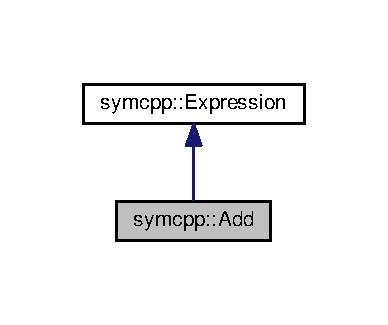
\includegraphics[width=186pt]{classsymcpp_1_1Add__inherit__graph}
\end{center}
\end{figure}


Collaboration diagram for symcpp\+:\+:Add\+:\nopagebreak
\begin{figure}[H]
\begin{center}
\leavevmode
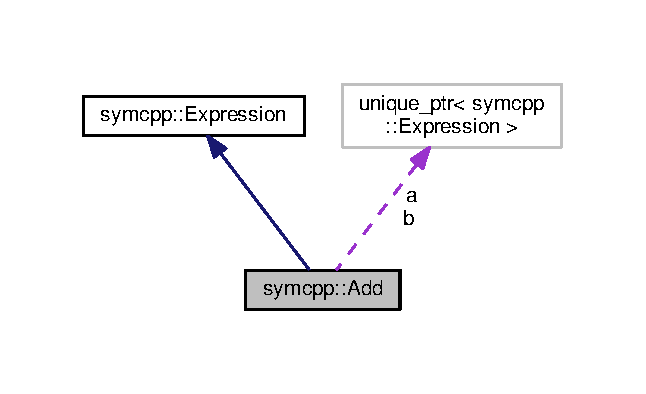
\includegraphics[width=310pt]{classsymcpp_1_1Add__coll__graph}
\end{center}
\end{figure}
\subsection*{Public Member Functions}
\begin{DoxyCompactItemize}
\item 
\hyperlink{classsymcpp_1_1Add_a037075ce08cb010b8873724279ebc9f7}{Add} (const \hyperlink{classsymcpp_1_1Expression}{Expression} \&\hyperlink{classsymcpp_1_1Add_a9c4fbbc6d99a6625e08e141d4f2bc615}{a}, const \hyperlink{classsymcpp_1_1Expression}{Expression} \&\hyperlink{classsymcpp_1_1Add_af79047cdc26b03c717544e86df5590a6}{b})
\item 
\hyperlink{classsymcpp_1_1Add_aee8c8948ed62d1d59d65053da6370caf}{Add} (std\+::unique\+\_\+ptr$<$ \hyperlink{classsymcpp_1_1Expression}{Expression} $>$ \&\&\hyperlink{classsymcpp_1_1Add_a9c4fbbc6d99a6625e08e141d4f2bc615}{a}, std\+::unique\+\_\+ptr$<$ \hyperlink{classsymcpp_1_1Expression}{Expression} $>$ \&\&\hyperlink{classsymcpp_1_1Add_af79047cdc26b03c717544e86df5590a6}{b})
\item 
double \hyperlink{classsymcpp_1_1Add_a79d0aa670728ba4a257e777ed4ac1ec0}{subs} (const std\+::unordered\+\_\+map$<$ std\+::string, double $>$ \&env) const override
\item 
std\+::unique\+\_\+ptr$<$ \hyperlink{classsymcpp_1_1Expression}{Expression} $>$ \hyperlink{classsymcpp_1_1Add_ac885da5635431d264c643618729f6cec}{diff} (std\+::string var) const override
\item 
std\+::unique\+\_\+ptr$<$ \hyperlink{classsymcpp_1_1Expression}{Expression} $>$ \hyperlink{classsymcpp_1_1Add_a58633f0c101ef1e7cc3952846054d27f}{copy} () const override
\item 
std\+::unique\+\_\+ptr$<$ \hyperlink{classsymcpp_1_1Expression}{Expression} $>$ \hyperlink{classsymcpp_1_1Add_a5a68fdd76c2206399dd5a78c4b317505}{simplify} () override
\item 
unsigned int \hyperlink{classsymcpp_1_1Add_aec3ebe2c1bde461d8bd086e9c87aeeed}{precedence} () const override
\item 
bool \hyperlink{classsymcpp_1_1Add_a6a9286402a1b24bf3a7c1ed348357875}{is\+\_\+constant} () const override
\item 
double \hyperlink{classsymcpp_1_1Add_af3e5c83af088ffc00849e852e18b055c}{const\+\_\+eval} () const override
\end{DoxyCompactItemize}
\subsection*{Private Member Functions}
\begin{DoxyCompactItemize}
\item 
std\+::ostream \& \hyperlink{classsymcpp_1_1Add_a4e73df4d72972d00ab139c5db4a93a0b}{print} (std\+::ostream \&sink) const override
\end{DoxyCompactItemize}
\subsection*{Private Attributes}
\begin{DoxyCompactItemize}
\item 
std\+::unique\+\_\+ptr$<$ \hyperlink{classsymcpp_1_1Expression}{Expression} $>$ \hyperlink{classsymcpp_1_1Add_a9c4fbbc6d99a6625e08e141d4f2bc615}{a}
\item 
std\+::unique\+\_\+ptr$<$ \hyperlink{classsymcpp_1_1Expression}{Expression} $>$ \hyperlink{classsymcpp_1_1Add_af79047cdc26b03c717544e86df5590a6}{b}
\end{DoxyCompactItemize}


\subsection{Constructor \& Destructor Documentation}
\index{symcpp\+::\+Add@{symcpp\+::\+Add}!Add@{Add}}
\index{Add@{Add}!symcpp\+::\+Add@{symcpp\+::\+Add}}
\subsubsection[{\texorpdfstring{Add(const Expression \&a, const Expression \&b)}{Add(const Expression &a, const Expression &b)}}]{\setlength{\rightskip}{0pt plus 5cm}symcpp\+::\+Add\+::\+Add (
\begin{DoxyParamCaption}
\item[{const {\bf Expression} \&}]{a, }
\item[{const {\bf Expression} \&}]{b}
\end{DoxyParamCaption}
)}\hypertarget{classsymcpp_1_1Add_a037075ce08cb010b8873724279ebc9f7}{}\label{classsymcpp_1_1Add_a037075ce08cb010b8873724279ebc9f7}
\index{symcpp\+::\+Add@{symcpp\+::\+Add}!Add@{Add}}
\index{Add@{Add}!symcpp\+::\+Add@{symcpp\+::\+Add}}
\subsubsection[{\texorpdfstring{Add(std\+::unique\+\_\+ptr$<$ Expression $>$ \&\&a, std\+::unique\+\_\+ptr$<$ Expression $>$ \&\&b)}{Add(std::unique_ptr< Expression > &&a, std::unique_ptr< Expression > &&b)}}]{\setlength{\rightskip}{0pt plus 5cm}symcpp\+::\+Add\+::\+Add (
\begin{DoxyParamCaption}
\item[{std\+::unique\+\_\+ptr$<$ {\bf Expression} $>$ \&\&}]{a, }
\item[{std\+::unique\+\_\+ptr$<$ {\bf Expression} $>$ \&\&}]{b}
\end{DoxyParamCaption}
)}\hypertarget{classsymcpp_1_1Add_aee8c8948ed62d1d59d65053da6370caf}{}\label{classsymcpp_1_1Add_aee8c8948ed62d1d59d65053da6370caf}


\subsection{Member Function Documentation}
\index{symcpp\+::\+Add@{symcpp\+::\+Add}!const\+\_\+eval@{const\+\_\+eval}}
\index{const\+\_\+eval@{const\+\_\+eval}!symcpp\+::\+Add@{symcpp\+::\+Add}}
\subsubsection[{\texorpdfstring{const\+\_\+eval() const override}{const_eval() const override}}]{\setlength{\rightskip}{0pt plus 5cm}double symcpp\+::\+Add\+::const\+\_\+eval (
\begin{DoxyParamCaption}
{}
\end{DoxyParamCaption}
) const\hspace{0.3cm}{\ttfamily [override]}, {\ttfamily [virtual]}}\hypertarget{classsymcpp_1_1Add_af3e5c83af088ffc00849e852e18b055c}{}\label{classsymcpp_1_1Add_af3e5c83af088ffc00849e852e18b055c}


Implements \hyperlink{classsymcpp_1_1Expression_a81c8069347f586cb5632338d97c278ad}{symcpp\+::\+Expression}.

\index{symcpp\+::\+Add@{symcpp\+::\+Add}!copy@{copy}}
\index{copy@{copy}!symcpp\+::\+Add@{symcpp\+::\+Add}}
\subsubsection[{\texorpdfstring{copy() const override}{copy() const override}}]{\setlength{\rightskip}{0pt plus 5cm}std\+::unique\+\_\+ptr$<$ {\bf Expression} $>$ symcpp\+::\+Add\+::copy (
\begin{DoxyParamCaption}
{}
\end{DoxyParamCaption}
) const\hspace{0.3cm}{\ttfamily [override]}, {\ttfamily [virtual]}}\hypertarget{classsymcpp_1_1Add_a58633f0c101ef1e7cc3952846054d27f}{}\label{classsymcpp_1_1Add_a58633f0c101ef1e7cc3952846054d27f}


Implements \hyperlink{classsymcpp_1_1Expression_a2e7de5a295ccf0efdc9b34cea7ba3d0b}{symcpp\+::\+Expression}.

\index{symcpp\+::\+Add@{symcpp\+::\+Add}!diff@{diff}}
\index{diff@{diff}!symcpp\+::\+Add@{symcpp\+::\+Add}}
\subsubsection[{\texorpdfstring{diff(std\+::string var) const override}{diff(std::string var) const override}}]{\setlength{\rightskip}{0pt plus 5cm}std\+::unique\+\_\+ptr$<$ {\bf Expression} $>$ symcpp\+::\+Add\+::diff (
\begin{DoxyParamCaption}
\item[{std\+::string}]{var}
\end{DoxyParamCaption}
) const\hspace{0.3cm}{\ttfamily [override]}, {\ttfamily [virtual]}}\hypertarget{classsymcpp_1_1Add_ac885da5635431d264c643618729f6cec}{}\label{classsymcpp_1_1Add_ac885da5635431d264c643618729f6cec}


Implements \hyperlink{classsymcpp_1_1Expression_a032fe8da79d5e231ca2d21a201c8f32d}{symcpp\+::\+Expression}.

\index{symcpp\+::\+Add@{symcpp\+::\+Add}!is\+\_\+constant@{is\+\_\+constant}}
\index{is\+\_\+constant@{is\+\_\+constant}!symcpp\+::\+Add@{symcpp\+::\+Add}}
\subsubsection[{\texorpdfstring{is\+\_\+constant() const override}{is_constant() const override}}]{\setlength{\rightskip}{0pt plus 5cm}bool symcpp\+::\+Add\+::is\+\_\+constant (
\begin{DoxyParamCaption}
{}
\end{DoxyParamCaption}
) const\hspace{0.3cm}{\ttfamily [override]}, {\ttfamily [virtual]}}\hypertarget{classsymcpp_1_1Add_a6a9286402a1b24bf3a7c1ed348357875}{}\label{classsymcpp_1_1Add_a6a9286402a1b24bf3a7c1ed348357875}


Implements \hyperlink{classsymcpp_1_1Expression_a30db7917c8948e22330cbe8259caeae2}{symcpp\+::\+Expression}.

\index{symcpp\+::\+Add@{symcpp\+::\+Add}!precedence@{precedence}}
\index{precedence@{precedence}!symcpp\+::\+Add@{symcpp\+::\+Add}}
\subsubsection[{\texorpdfstring{precedence() const override}{precedence() const override}}]{\setlength{\rightskip}{0pt plus 5cm}unsigned int symcpp\+::\+Add\+::precedence (
\begin{DoxyParamCaption}
{}
\end{DoxyParamCaption}
) const\hspace{0.3cm}{\ttfamily [override]}, {\ttfamily [virtual]}}\hypertarget{classsymcpp_1_1Add_aec3ebe2c1bde461d8bd086e9c87aeeed}{}\label{classsymcpp_1_1Add_aec3ebe2c1bde461d8bd086e9c87aeeed}


Implements \hyperlink{classsymcpp_1_1Expression_a181c162d5740faac392ffdca26bfca0c}{symcpp\+::\+Expression}.

\index{symcpp\+::\+Add@{symcpp\+::\+Add}!print@{print}}
\index{print@{print}!symcpp\+::\+Add@{symcpp\+::\+Add}}
\subsubsection[{\texorpdfstring{print(std\+::ostream \&sink) const override}{print(std::ostream &sink) const override}}]{\setlength{\rightskip}{0pt plus 5cm}std\+::ostream \& symcpp\+::\+Add\+::print (
\begin{DoxyParamCaption}
\item[{std\+::ostream \&}]{sink}
\end{DoxyParamCaption}
) const\hspace{0.3cm}{\ttfamily [override]}, {\ttfamily [private]}, {\ttfamily [virtual]}}\hypertarget{classsymcpp_1_1Add_a4e73df4d72972d00ab139c5db4a93a0b}{}\label{classsymcpp_1_1Add_a4e73df4d72972d00ab139c5db4a93a0b}


Implements \hyperlink{classsymcpp_1_1Expression_af37e13032a40f2da4d2866eaa8658049}{symcpp\+::\+Expression}.

\index{symcpp\+::\+Add@{symcpp\+::\+Add}!simplify@{simplify}}
\index{simplify@{simplify}!symcpp\+::\+Add@{symcpp\+::\+Add}}
\subsubsection[{\texorpdfstring{simplify() override}{simplify() override}}]{\setlength{\rightskip}{0pt plus 5cm}std\+::unique\+\_\+ptr$<$ {\bf Expression} $>$ symcpp\+::\+Add\+::simplify (
\begin{DoxyParamCaption}
{}
\end{DoxyParamCaption}
)\hspace{0.3cm}{\ttfamily [override]}, {\ttfamily [virtual]}}\hypertarget{classsymcpp_1_1Add_a5a68fdd76c2206399dd5a78c4b317505}{}\label{classsymcpp_1_1Add_a5a68fdd76c2206399dd5a78c4b317505}


Implements \hyperlink{classsymcpp_1_1Expression_ab1fa6e55eea0682250d013f28db26cd2}{symcpp\+::\+Expression}.

\index{symcpp\+::\+Add@{symcpp\+::\+Add}!subs@{subs}}
\index{subs@{subs}!symcpp\+::\+Add@{symcpp\+::\+Add}}
\subsubsection[{\texorpdfstring{subs(const std\+::unordered\+\_\+map$<$ std\+::string, double $>$ \&env) const override}{subs(const std::unordered_map< std::string, double > &env) const override}}]{\setlength{\rightskip}{0pt plus 5cm}double symcpp\+::\+Add\+::subs (
\begin{DoxyParamCaption}
\item[{const std\+::unordered\+\_\+map$<$ std\+::string, double $>$ \&}]{env}
\end{DoxyParamCaption}
) const\hspace{0.3cm}{\ttfamily [override]}, {\ttfamily [virtual]}}\hypertarget{classsymcpp_1_1Add_a79d0aa670728ba4a257e777ed4ac1ec0}{}\label{classsymcpp_1_1Add_a79d0aa670728ba4a257e777ed4ac1ec0}


Implements \hyperlink{classsymcpp_1_1Expression_aaef29b0afa2d6c21fe35f47a1be76134}{symcpp\+::\+Expression}.



\subsection{Member Data Documentation}
\index{symcpp\+::\+Add@{symcpp\+::\+Add}!a@{a}}
\index{a@{a}!symcpp\+::\+Add@{symcpp\+::\+Add}}
\subsubsection[{\texorpdfstring{a}{a}}]{\setlength{\rightskip}{0pt plus 5cm}std\+::unique\+\_\+ptr$<${\bf Expression}$>$ symcpp\+::\+Add\+::a\hspace{0.3cm}{\ttfamily [private]}}\hypertarget{classsymcpp_1_1Add_a9c4fbbc6d99a6625e08e141d4f2bc615}{}\label{classsymcpp_1_1Add_a9c4fbbc6d99a6625e08e141d4f2bc615}
\index{symcpp\+::\+Add@{symcpp\+::\+Add}!b@{b}}
\index{b@{b}!symcpp\+::\+Add@{symcpp\+::\+Add}}
\subsubsection[{\texorpdfstring{b}{b}}]{\setlength{\rightskip}{0pt plus 5cm}std\+::unique\+\_\+ptr$<${\bf Expression}$>$ symcpp\+::\+Add\+::b\hspace{0.3cm}{\ttfamily [private]}}\hypertarget{classsymcpp_1_1Add_af79047cdc26b03c717544e86df5590a6}{}\label{classsymcpp_1_1Add_af79047cdc26b03c717544e86df5590a6}


The documentation for this class was generated from the following files\+:\begin{DoxyCompactItemize}
\item 
src/symcpp/\hyperlink{Add_8h}{Add.\+h}\item 
src/symcpp/\hyperlink{Add_8cpp}{Add.\+cpp}\end{DoxyCompactItemize}

\hypertarget{classBackground}{}\section{Background Class Reference}
\label{classBackground}\index{Background@{Background}}


{\ttfamily \#include $<$Background.\+h$>$}



Collaboration diagram for Background\+:\nopagebreak
\begin{figure}[H]
\begin{center}
\leavevmode
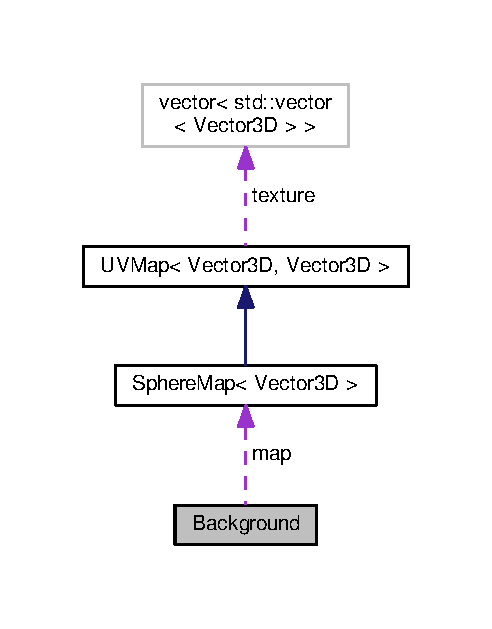
\includegraphics[width=236pt]{classBackground__coll__graph}
\end{center}
\end{figure}
\subsection*{Public Member Functions}
\begin{DoxyCompactItemize}
\item 
\hyperlink{classBackground_a153fe3ce08c90c24e7d08862952a6244}{Background} (\hyperlink{classVector3D}{Vector3D} c)
\item 
\hyperlink{classBackground_a46cb4a8649d0d0535c916eea458c25de}{Background} (const \hyperlink{classSphereMap}{Sphere\+Map}$<$ \hyperlink{classVector3D}{Vector3D} $>$ \&im)
\item 
\hyperlink{classVector3D}{Vector3D} \hyperlink{classBackground_a901242466450821f487a1967d94c6506}{get\+Color} (\hyperlink{classVector3D}{Vector3D} coordinates)
\end{DoxyCompactItemize}
\subsection*{Private Attributes}
\begin{DoxyCompactItemize}
\item 
\hyperlink{classSphereMap}{Sphere\+Map}$<$ \hyperlink{classVector3D}{Vector3D} $>$ \hyperlink{classBackground_af0f03647aa08a06ba2a2105832c2097c}{map}
\end{DoxyCompactItemize}


\subsection{Constructor \& Destructor Documentation}
\index{Background@{Background}!Background@{Background}}
\index{Background@{Background}!Background@{Background}}
\subsubsection[{\texorpdfstring{Background(\+Vector3\+D c)}{Background(Vector3D c)}}]{\setlength{\rightskip}{0pt plus 5cm}Background\+::\+Background (
\begin{DoxyParamCaption}
\item[{{\bf Vector3D}}]{c}
\end{DoxyParamCaption}
)\hspace{0.3cm}{\ttfamily [explicit]}}\hypertarget{classBackground_a153fe3ce08c90c24e7d08862952a6244}{}\label{classBackground_a153fe3ce08c90c24e7d08862952a6244}
\index{Background@{Background}!Background@{Background}}
\index{Background@{Background}!Background@{Background}}
\subsubsection[{\texorpdfstring{Background(const Sphere\+Map$<$ Vector3\+D $>$ \&im)}{Background(const SphereMap< Vector3D > &im)}}]{\setlength{\rightskip}{0pt plus 5cm}Background\+::\+Background (
\begin{DoxyParamCaption}
\item[{const {\bf Sphere\+Map}$<$ {\bf Vector3D} $>$ \&}]{im}
\end{DoxyParamCaption}
)\hspace{0.3cm}{\ttfamily [explicit]}}\hypertarget{classBackground_a46cb4a8649d0d0535c916eea458c25de}{}\label{classBackground_a46cb4a8649d0d0535c916eea458c25de}


\subsection{Member Function Documentation}
\index{Background@{Background}!get\+Color@{get\+Color}}
\index{get\+Color@{get\+Color}!Background@{Background}}
\subsubsection[{\texorpdfstring{get\+Color(\+Vector3\+D coordinates)}{getColor(Vector3D coordinates)}}]{\setlength{\rightskip}{0pt plus 5cm}{\bf Vector3D} Background\+::get\+Color (
\begin{DoxyParamCaption}
\item[{{\bf Vector3D}}]{coordinates}
\end{DoxyParamCaption}
)}\hypertarget{classBackground_a901242466450821f487a1967d94c6506}{}\label{classBackground_a901242466450821f487a1967d94c6506}


\subsection{Member Data Documentation}
\index{Background@{Background}!map@{map}}
\index{map@{map}!Background@{Background}}
\subsubsection[{\texorpdfstring{map}{map}}]{\setlength{\rightskip}{0pt plus 5cm}{\bf Sphere\+Map}$<${\bf Vector3D}$>$ Background\+::map\hspace{0.3cm}{\ttfamily [private]}}\hypertarget{classBackground_af0f03647aa08a06ba2a2105832c2097c}{}\label{classBackground_af0f03647aa08a06ba2a2105832c2097c}


The documentation for this class was generated from the following files\+:\begin{DoxyCompactItemize}
\item 
src/\hyperlink{Background_8h}{Background.\+h}\item 
src/\hyperlink{Background_8cpp}{Background.\+cpp}\end{DoxyCompactItemize}

\hypertarget{classBinaryVolumeHierarchy}{}\section{Binary\+Volume\+Hierarchy Class Reference}
\label{classBinaryVolumeHierarchy}\index{Binary\+Volume\+Hierarchy@{Binary\+Volume\+Hierarchy}}


Accelerationstructure for ensemble of bounded volumes.  




{\ttfamily \#include $<$Binary\+Volume\+Hierarchy.\+h$>$}



Inheritance diagram for Binary\+Volume\+Hierarchy\+:\nopagebreak
\begin{figure}[H]
\begin{center}
\leavevmode
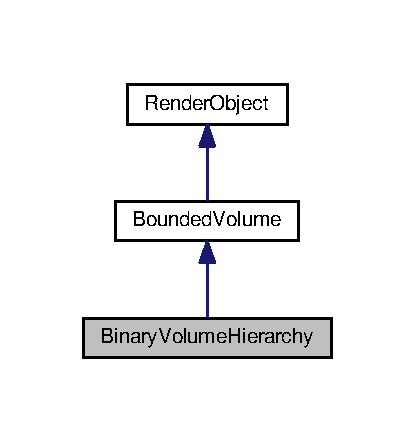
\includegraphics[width=199pt]{classBinaryVolumeHierarchy__inherit__graph}
\end{center}
\end{figure}


Collaboration diagram for Binary\+Volume\+Hierarchy\+:\nopagebreak
\begin{figure}[H]
\begin{center}
\leavevmode
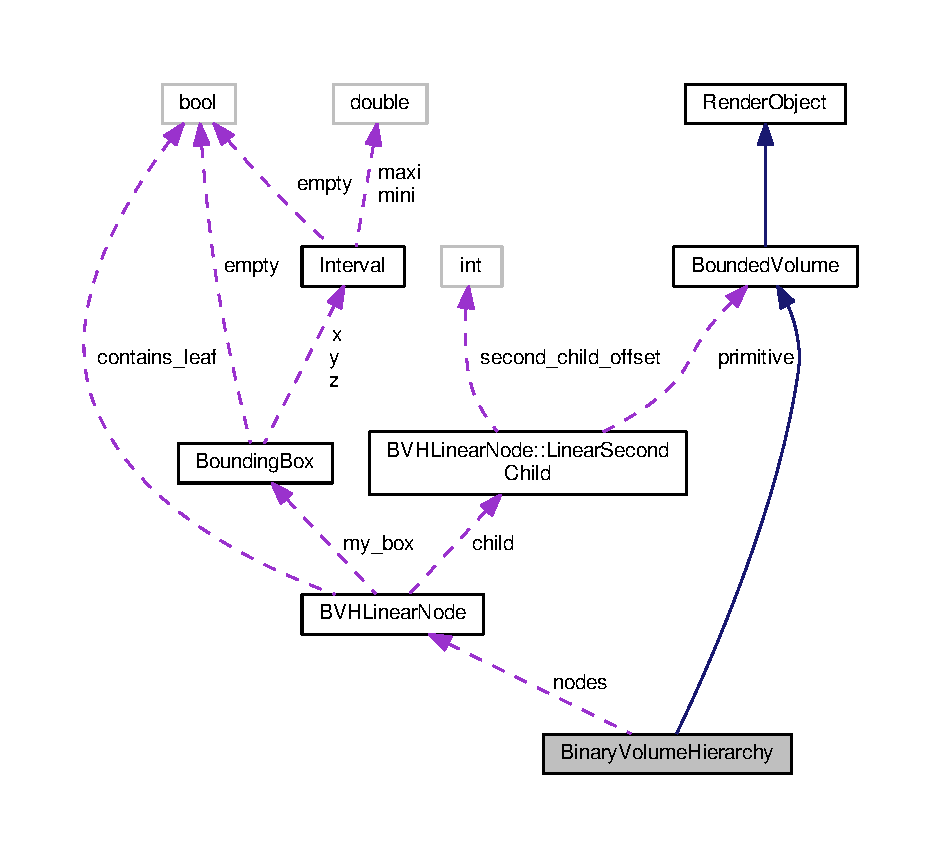
\includegraphics[width=335pt]{classBinaryVolumeHierarchy__coll__graph}
\end{center}
\end{figure}
\subsection*{Public Member Functions}
\begin{DoxyCompactItemize}
\item 
\hyperlink{classBinaryVolumeHierarchy_afb1953933b78a2005884a7a34cb64519}{Binary\+Volume\+Hierarchy} (std\+::vector$<$ \hyperlink{classBoundedVolume}{Bounded\+Volume} $\ast$ $>$\+::iterator b, std\+::vector$<$ \hyperlink{classBoundedVolume}{Bounded\+Volume} $\ast$ $>$\+::iterator e)
\item 
\hyperlink{classBinaryVolumeHierarchy_a4a45b2c778163d01304beb57b6d19bd3}{Binary\+Volume\+Hierarchy} (const \hyperlink{classBinaryVolumeHierarchy}{Binary\+Volume\+Hierarchy} \&other)
\item 
\hyperlink{classBinaryVolumeHierarchy}{Binary\+Volume\+Hierarchy} \& \hyperlink{classBinaryVolumeHierarchy_af15afa9493fbc0d3cfffbbc3c2bfbe99}{operator=} (\hyperlink{classBinaryVolumeHierarchy}{Binary\+Volume\+Hierarchy} other)
\item 
\hyperlink{classIntersection}{Intersection} \hyperlink{classBinaryVolumeHierarchy_a1eda3a8f9a52d44cd483d9bc2807b38a}{ray\+Intersect} (const \hyperlink{classRay}{Ray} \&ray) const override
\begin{DoxyCompactList}\small\item\em Method to detect intersection of ray and object. \end{DoxyCompactList}\item 
\hyperlink{classBoundingBox}{Bounding\+Box} \hyperlink{classBinaryVolumeHierarchy_af4875ad00fe5c6430067e00647918b5a}{get\+Bounds} () const override
\item 
std\+::ostream \& \hyperlink{classBinaryVolumeHierarchy_ad92d27372aef59591ddc239685ca770d}{print} (std\+::ostream \&sink) const override
\item 
\hyperlink{classIntersectionProperties}{Intersection\+Properties} \hyperlink{classBinaryVolumeHierarchy_af3c2277401a26961295a2b0ac18b1dd4}{intersect\+Properties} (const \hyperlink{classRay}{Ray} \&ray) const override
\begin{DoxyCompactList}\small\item\em If ray intersects this object, this method will provide additional Information. \end{DoxyCompactList}\item 
\hyperlink{classBinaryVolumeHierarchy_a760800685de78279be3619c4ee4170cf}{$\sim$\+Binary\+Volume\+Hierarchy} () override
\end{DoxyCompactItemize}
\subsection*{Private Member Functions}
\begin{DoxyCompactItemize}
\item 
std\+::vector$<$ \hyperlink{classBoundedVolume}{Bounded\+Volume} $\ast$ $>$\+::iterator \hyperlink{classBinaryVolumeHierarchy_ab30dec4aa6ef808f53bbdedb98d8af65}{partition} (std\+::vector$<$ \hyperlink{classBoundedVolume}{Bounded\+Volume} $\ast$ $>$\+::iterator b, std\+::vector$<$ \hyperlink{classBoundedVolume}{Bounded\+Volume} $\ast$ $>$\+::iterator e)
\item 
unsigned int \hyperlink{classBinaryVolumeHierarchy_a93e3d7fd0b06a83675e36594d3fcaa8b}{longest\+Axis} () const 
\end{DoxyCompactItemize}
\subsection*{Private Attributes}
\begin{DoxyCompactItemize}
\item 
\hyperlink{structBVHNode}{B\+V\+H\+Node} $\ast$ \hyperlink{classBinaryVolumeHierarchy_a76372fd6f7d6a5783d9b8688fc40d5b4}{left}
\item 
\hyperlink{structBVHNode}{B\+V\+H\+Node} $\ast$ \hyperlink{classBinaryVolumeHierarchy_a3b950d10a084fedfeaa02727d654b782}{right}
\item 
\hyperlink{classBoundingBox}{Bounding\+Box} \hyperlink{classBinaryVolumeHierarchy_a2722a35a0c3c6fee488f186c31869b53}{bounds}
\end{DoxyCompactItemize}


\subsection{Detailed Description}
Accelerationstructure for ensemble of bounded volumes. 

\subsection{Constructor \& Destructor Documentation}
\index{Binary\+Volume\+Hierarchy@{Binary\+Volume\+Hierarchy}!Binary\+Volume\+Hierarchy@{Binary\+Volume\+Hierarchy}}
\index{Binary\+Volume\+Hierarchy@{Binary\+Volume\+Hierarchy}!Binary\+Volume\+Hierarchy@{Binary\+Volume\+Hierarchy}}
\subsubsection[{\texorpdfstring{Binary\+Volume\+Hierarchy(std\+::vector$<$ Bounded\+Volume $\ast$ $>$\+::iterator b, std\+::vector$<$ Bounded\+Volume $\ast$ $>$\+::iterator e)}{BinaryVolumeHierarchy(std::vector< BoundedVolume * >::iterator b, std::vector< BoundedVolume * >::iterator e)}}]{\setlength{\rightskip}{0pt plus 5cm}Binary\+Volume\+Hierarchy\+::\+Binary\+Volume\+Hierarchy (
\begin{DoxyParamCaption}
\item[{std\+::vector$<$ {\bf Bounded\+Volume} $\ast$ $>$\+::iterator}]{b, }
\item[{std\+::vector$<$ {\bf Bounded\+Volume} $\ast$ $>$\+::iterator}]{e}
\end{DoxyParamCaption}
)}\hypertarget{classBinaryVolumeHierarchy_afb1953933b78a2005884a7a34cb64519}{}\label{classBinaryVolumeHierarchy_afb1953933b78a2005884a7a34cb64519}
\index{Binary\+Volume\+Hierarchy@{Binary\+Volume\+Hierarchy}!Binary\+Volume\+Hierarchy@{Binary\+Volume\+Hierarchy}}
\index{Binary\+Volume\+Hierarchy@{Binary\+Volume\+Hierarchy}!Binary\+Volume\+Hierarchy@{Binary\+Volume\+Hierarchy}}
\subsubsection[{\texorpdfstring{Binary\+Volume\+Hierarchy(const Binary\+Volume\+Hierarchy \&other)}{BinaryVolumeHierarchy(const BinaryVolumeHierarchy &other)}}]{\setlength{\rightskip}{0pt plus 5cm}Binary\+Volume\+Hierarchy\+::\+Binary\+Volume\+Hierarchy (
\begin{DoxyParamCaption}
\item[{const {\bf Binary\+Volume\+Hierarchy} \&}]{other}
\end{DoxyParamCaption}
)}\hypertarget{classBinaryVolumeHierarchy_a4a45b2c778163d01304beb57b6d19bd3}{}\label{classBinaryVolumeHierarchy_a4a45b2c778163d01304beb57b6d19bd3}
\index{Binary\+Volume\+Hierarchy@{Binary\+Volume\+Hierarchy}!````~Binary\+Volume\+Hierarchy@{$\sim$\+Binary\+Volume\+Hierarchy}}
\index{````~Binary\+Volume\+Hierarchy@{$\sim$\+Binary\+Volume\+Hierarchy}!Binary\+Volume\+Hierarchy@{Binary\+Volume\+Hierarchy}}
\subsubsection[{\texorpdfstring{$\sim$\+Binary\+Volume\+Hierarchy() override}{~BinaryVolumeHierarchy() override}}]{\setlength{\rightskip}{0pt plus 5cm}Binary\+Volume\+Hierarchy\+::$\sim$\+Binary\+Volume\+Hierarchy (
\begin{DoxyParamCaption}
{}
\end{DoxyParamCaption}
)\hspace{0.3cm}{\ttfamily [override]}}\hypertarget{classBinaryVolumeHierarchy_a760800685de78279be3619c4ee4170cf}{}\label{classBinaryVolumeHierarchy_a760800685de78279be3619c4ee4170cf}


\subsection{Member Function Documentation}
\index{Binary\+Volume\+Hierarchy@{Binary\+Volume\+Hierarchy}!get\+Bounds@{get\+Bounds}}
\index{get\+Bounds@{get\+Bounds}!Binary\+Volume\+Hierarchy@{Binary\+Volume\+Hierarchy}}
\subsubsection[{\texorpdfstring{get\+Bounds() const override}{getBounds() const override}}]{\setlength{\rightskip}{0pt plus 5cm}{\bf Bounding\+Box} Binary\+Volume\+Hierarchy\+::get\+Bounds (
\begin{DoxyParamCaption}
{}
\end{DoxyParamCaption}
) const\hspace{0.3cm}{\ttfamily [override]}, {\ttfamily [virtual]}}\hypertarget{classBinaryVolumeHierarchy_af4875ad00fe5c6430067e00647918b5a}{}\label{classBinaryVolumeHierarchy_af4875ad00fe5c6430067e00647918b5a}


Implements \hyperlink{classBoundedVolume_a3d912b7028f7046fe18c4edf3a400e3b}{Bounded\+Volume}.

\index{Binary\+Volume\+Hierarchy@{Binary\+Volume\+Hierarchy}!intersect\+Properties@{intersect\+Properties}}
\index{intersect\+Properties@{intersect\+Properties}!Binary\+Volume\+Hierarchy@{Binary\+Volume\+Hierarchy}}
\subsubsection[{\texorpdfstring{intersect\+Properties(const Ray \&ray) const override}{intersectProperties(const Ray &ray) const override}}]{\setlength{\rightskip}{0pt plus 5cm}{\bf Intersection\+Properties} Binary\+Volume\+Hierarchy\+::intersect\+Properties (
\begin{DoxyParamCaption}
\item[{const {\bf Ray} \&}]{ray}
\end{DoxyParamCaption}
) const\hspace{0.3cm}{\ttfamily [override]}, {\ttfamily [virtual]}}\hypertarget{classBinaryVolumeHierarchy_af3c2277401a26961295a2b0ac18b1dd4}{}\label{classBinaryVolumeHierarchy_af3c2277401a26961295a2b0ac18b1dd4}


If ray intersects this object, this method will provide additional Information. 

Note, that even if ray\+Intersect detected an intersection, this method might not be called. It is called iff the Intersection-\/\+Object returned by ray\+Intersect contains a pointer to this object and no other object in the rendered scene returned an intersection that was closer to the camera.


\begin{DoxyParams}{Parameters}
{\em ray} & the ray in question \\
\hline
\end{DoxyParams}
\begin{DoxyReturn}{Returns}
\hyperlink{classIntersectionProperties}{Intersection\+Properties} object containing the surface normal and material information 
\end{DoxyReturn}


Implements \hyperlink{classRenderObject_ae2c6d699741385dcd9ea6a1b09f9b7f0}{Render\+Object}.

\index{Binary\+Volume\+Hierarchy@{Binary\+Volume\+Hierarchy}!longest\+Axis@{longest\+Axis}}
\index{longest\+Axis@{longest\+Axis}!Binary\+Volume\+Hierarchy@{Binary\+Volume\+Hierarchy}}
\subsubsection[{\texorpdfstring{longest\+Axis() const }{longestAxis() const }}]{\setlength{\rightskip}{0pt plus 5cm}unsigned int Binary\+Volume\+Hierarchy\+::longest\+Axis (
\begin{DoxyParamCaption}
{}
\end{DoxyParamCaption}
) const\hspace{0.3cm}{\ttfamily [private]}}\hypertarget{classBinaryVolumeHierarchy_a93e3d7fd0b06a83675e36594d3fcaa8b}{}\label{classBinaryVolumeHierarchy_a93e3d7fd0b06a83675e36594d3fcaa8b}
\index{Binary\+Volume\+Hierarchy@{Binary\+Volume\+Hierarchy}!operator=@{operator=}}
\index{operator=@{operator=}!Binary\+Volume\+Hierarchy@{Binary\+Volume\+Hierarchy}}
\subsubsection[{\texorpdfstring{operator=(\+Binary\+Volume\+Hierarchy other)}{operator=(BinaryVolumeHierarchy other)}}]{\setlength{\rightskip}{0pt plus 5cm}{\bf Binary\+Volume\+Hierarchy} \& Binary\+Volume\+Hierarchy\+::operator= (
\begin{DoxyParamCaption}
\item[{{\bf Binary\+Volume\+Hierarchy}}]{other}
\end{DoxyParamCaption}
)}\hypertarget{classBinaryVolumeHierarchy_af15afa9493fbc0d3cfffbbc3c2bfbe99}{}\label{classBinaryVolumeHierarchy_af15afa9493fbc0d3cfffbbc3c2bfbe99}
\index{Binary\+Volume\+Hierarchy@{Binary\+Volume\+Hierarchy}!partition@{partition}}
\index{partition@{partition}!Binary\+Volume\+Hierarchy@{Binary\+Volume\+Hierarchy}}
\subsubsection[{\texorpdfstring{partition(std\+::vector$<$ Bounded\+Volume $\ast$ $>$\+::iterator b, std\+::vector$<$ Bounded\+Volume $\ast$ $>$\+::iterator e)}{partition(std::vector< BoundedVolume * >::iterator b, std::vector< BoundedVolume * >::iterator e)}}]{\setlength{\rightskip}{0pt plus 5cm}std\+::vector$<$ {\bf Bounded\+Volume} $\ast$ $>$\+::iterator Binary\+Volume\+Hierarchy\+::partition (
\begin{DoxyParamCaption}
\item[{std\+::vector$<$ {\bf Bounded\+Volume} $\ast$ $>$\+::iterator}]{b, }
\item[{std\+::vector$<$ {\bf Bounded\+Volume} $\ast$ $>$\+::iterator}]{e}
\end{DoxyParamCaption}
)\hspace{0.3cm}{\ttfamily [private]}}\hypertarget{classBinaryVolumeHierarchy_ab30dec4aa6ef808f53bbdedb98d8af65}{}\label{classBinaryVolumeHierarchy_ab30dec4aa6ef808f53bbdedb98d8af65}
\index{Binary\+Volume\+Hierarchy@{Binary\+Volume\+Hierarchy}!print@{print}}
\index{print@{print}!Binary\+Volume\+Hierarchy@{Binary\+Volume\+Hierarchy}}
\subsubsection[{\texorpdfstring{print(std\+::ostream \&sink) const override}{print(std::ostream &sink) const override}}]{\setlength{\rightskip}{0pt plus 5cm}std\+::ostream \& Binary\+Volume\+Hierarchy\+::print (
\begin{DoxyParamCaption}
\item[{std\+::ostream \&}]{sink}
\end{DoxyParamCaption}
) const\hspace{0.3cm}{\ttfamily [override]}, {\ttfamily [virtual]}}\hypertarget{classBinaryVolumeHierarchy_ad92d27372aef59591ddc239685ca770d}{}\label{classBinaryVolumeHierarchy_ad92d27372aef59591ddc239685ca770d}


Implements \hyperlink{classRenderObject_a7a7f1168a7d96ca95235b170ff7fb11b}{Render\+Object}.

\index{Binary\+Volume\+Hierarchy@{Binary\+Volume\+Hierarchy}!ray\+Intersect@{ray\+Intersect}}
\index{ray\+Intersect@{ray\+Intersect}!Binary\+Volume\+Hierarchy@{Binary\+Volume\+Hierarchy}}
\subsubsection[{\texorpdfstring{ray\+Intersect(const Ray \&ray) const override}{rayIntersect(const Ray &ray) const override}}]{\setlength{\rightskip}{0pt plus 5cm}{\bf Intersection} Binary\+Volume\+Hierarchy\+::ray\+Intersect (
\begin{DoxyParamCaption}
\item[{const {\bf Ray} \&}]{ray}
\end{DoxyParamCaption}
) const\hspace{0.3cm}{\ttfamily [override]}, {\ttfamily [virtual]}}\hypertarget{classBinaryVolumeHierarchy_a1eda3a8f9a52d44cd483d9bc2807b38a}{}\label{classBinaryVolumeHierarchy_a1eda3a8f9a52d44cd483d9bc2807b38a}


Method to detect intersection of ray and object. 


\begin{DoxyParams}{Parameters}
{\em ray} & The ray in question \\
\hline
\end{DoxyParams}
\begin{DoxyReturn}{Returns}
\hyperlink{classIntersection}{Intersection} object containing distance to intersection and pointer to intersected object 
\end{DoxyReturn}


Implements \hyperlink{classRenderObject_a681f6674d94f16c4df69605d5e42d05c}{Render\+Object}.



\subsection{Member Data Documentation}
\index{Binary\+Volume\+Hierarchy@{Binary\+Volume\+Hierarchy}!bounds@{bounds}}
\index{bounds@{bounds}!Binary\+Volume\+Hierarchy@{Binary\+Volume\+Hierarchy}}
\subsubsection[{\texorpdfstring{bounds}{bounds}}]{\setlength{\rightskip}{0pt plus 5cm}{\bf Bounding\+Box} Binary\+Volume\+Hierarchy\+::bounds\hspace{0.3cm}{\ttfamily [private]}}\hypertarget{classBinaryVolumeHierarchy_a2722a35a0c3c6fee488f186c31869b53}{}\label{classBinaryVolumeHierarchy_a2722a35a0c3c6fee488f186c31869b53}
\index{Binary\+Volume\+Hierarchy@{Binary\+Volume\+Hierarchy}!left@{left}}
\index{left@{left}!Binary\+Volume\+Hierarchy@{Binary\+Volume\+Hierarchy}}
\subsubsection[{\texorpdfstring{left}{left}}]{\setlength{\rightskip}{0pt plus 5cm}{\bf B\+V\+H\+Node}$\ast$ Binary\+Volume\+Hierarchy\+::left\hspace{0.3cm}{\ttfamily [private]}}\hypertarget{classBinaryVolumeHierarchy_a76372fd6f7d6a5783d9b8688fc40d5b4}{}\label{classBinaryVolumeHierarchy_a76372fd6f7d6a5783d9b8688fc40d5b4}
\index{Binary\+Volume\+Hierarchy@{Binary\+Volume\+Hierarchy}!right@{right}}
\index{right@{right}!Binary\+Volume\+Hierarchy@{Binary\+Volume\+Hierarchy}}
\subsubsection[{\texorpdfstring{right}{right}}]{\setlength{\rightskip}{0pt plus 5cm}{\bf B\+V\+H\+Node}$\ast$ Binary\+Volume\+Hierarchy\+::right\hspace{0.3cm}{\ttfamily [private]}}\hypertarget{classBinaryVolumeHierarchy_a3b950d10a084fedfeaa02727d654b782}{}\label{classBinaryVolumeHierarchy_a3b950d10a084fedfeaa02727d654b782}


The documentation for this class was generated from the following files\+:\begin{DoxyCompactItemize}
\item 
src/\hyperlink{BinaryVolumeHierarchy_8h}{Binary\+Volume\+Hierarchy.\+h}\item 
src/\hyperlink{BinaryVolumeHierarchy_8cpp}{Binary\+Volume\+Hierarchy.\+cpp}\end{DoxyCompactItemize}

\hypertarget{classBoundedVolume}{}\section{Bounded\+Volume Class Reference}
\label{classBoundedVolume}\index{Bounded\+Volume@{Bounded\+Volume}}


Abstract class implemented by objects that can be contained in a volume.  




{\ttfamily \#include $<$Bounded\+Volume.\+h$>$}



Inheritance diagram for Bounded\+Volume\+:\nopagebreak
\begin{figure}[H]
\begin{center}
\leavevmode
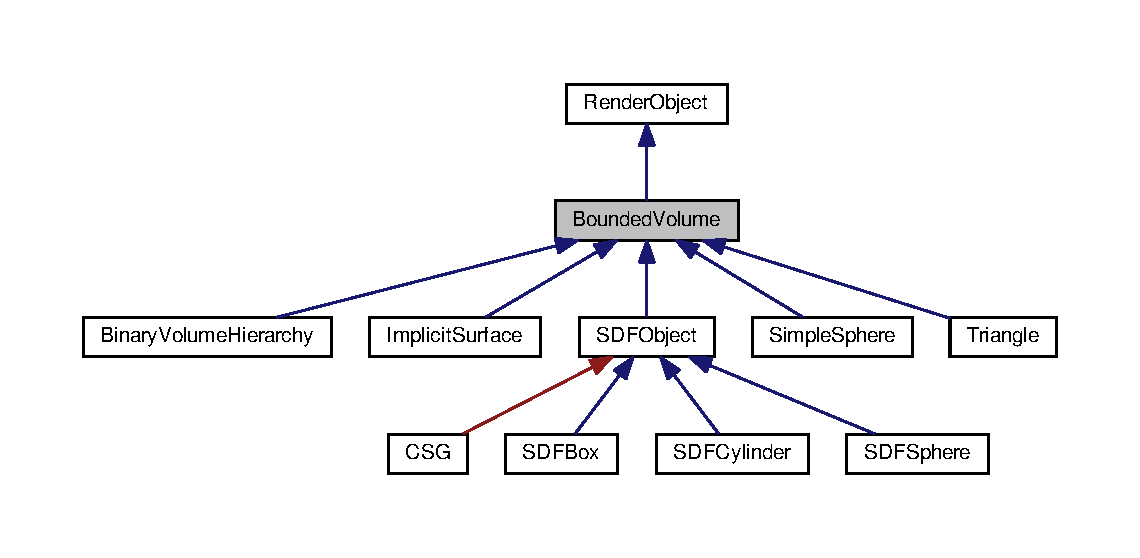
\includegraphics[width=350pt]{classBoundedVolume__inherit__graph}
\end{center}
\end{figure}


Collaboration diagram for Bounded\+Volume\+:\nopagebreak
\begin{figure}[H]
\begin{center}
\leavevmode
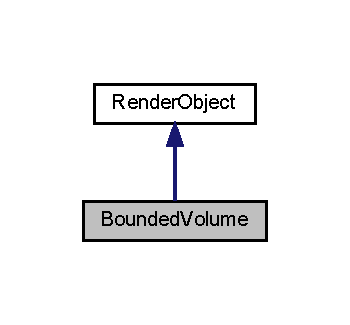
\includegraphics[width=168pt]{classBoundedVolume__coll__graph}
\end{center}
\end{figure}
\subsection*{Public Member Functions}
\begin{DoxyCompactItemize}
\item 
virtual \hyperlink{classBoundingBox}{Bounding\+Box} \hyperlink{classBoundedVolume_a281168c4d827c38b46e639f6e4991a9e}{get\+\_\+bounds} () const =0
\end{DoxyCompactItemize}


\subsection{Detailed Description}
Abstract class implemented by objects that can be contained in a volume. 

\subsection{Member Function Documentation}
\index{Bounded\+Volume@{Bounded\+Volume}!get\+\_\+bounds@{get\+\_\+bounds}}
\index{get\+\_\+bounds@{get\+\_\+bounds}!Bounded\+Volume@{Bounded\+Volume}}
\subsubsection[{\texorpdfstring{get\+\_\+bounds() const =0}{get_bounds() const =0}}]{\setlength{\rightskip}{0pt plus 5cm}virtual {\bf Bounding\+Box} Bounded\+Volume\+::get\+\_\+bounds (
\begin{DoxyParamCaption}
{}
\end{DoxyParamCaption}
) const\hspace{0.3cm}{\ttfamily [pure virtual]}}\hypertarget{classBoundedVolume_a281168c4d827c38b46e639f6e4991a9e}{}\label{classBoundedVolume_a281168c4d827c38b46e639f6e4991a9e}


Implemented in \hyperlink{classImplicitSurface_a30f0b97eb9976f8e40be7b990d6352d6}{Implicit\+Surface}, \hyperlink{classBinaryVolumeHierarchy_aaec23515bc9d81ccc9115489aed8808f}{Binary\+Volume\+Hierarchy}, \hyperlink{classSimpleSphere_aa5b6b2ebbe3de4490cdaa0f5c08b961c}{Simple\+Sphere}, and \hyperlink{classTriangle_ac93216ac2308504ab7dd7679e6b84937}{Triangle}.



The documentation for this class was generated from the following file\+:\begin{DoxyCompactItemize}
\item 
src/\hyperlink{BoundedVolume_8h}{Bounded\+Volume.\+h}\end{DoxyCompactItemize}

\hypertarget{classBoundingBox}{}\section{Bounding\+Box Class Reference}
\label{classBoundingBox}\index{Bounding\+Box@{Bounding\+Box}}


A cuboid in 3D space for estimating the position of objects.  




{\ttfamily \#include $<$Bounding\+Box.\+h$>$}



Collaboration diagram for Bounding\+Box\+:\nopagebreak
\begin{figure}[H]
\begin{center}
\leavevmode
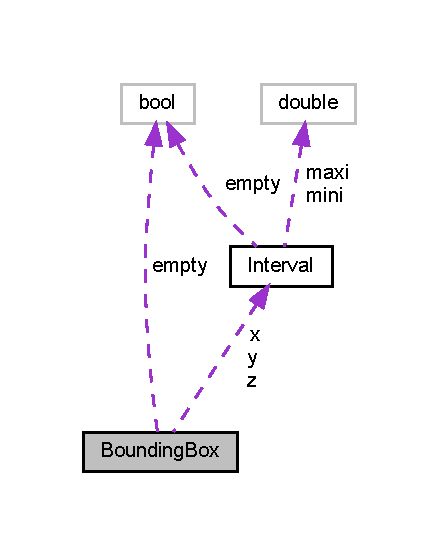
\includegraphics[width=201pt]{classBoundingBox__coll__graph}
\end{center}
\end{figure}
\subsection*{Public Member Functions}
\begin{DoxyCompactItemize}
\item 
\hyperlink{classBoundingBox_a4120184a9340ea9a0c43285c9d0f18bf}{Bounding\+Box} (\hyperlink{classInterval}{Interval} \hyperlink{classBoundingBox_a93ea5f12ef2300fe61925f6b44faaebe}{x}, \hyperlink{classInterval}{Interval} \hyperlink{classBoundingBox_a593fd6b66d3ed0352d92024685863090}{y}, \hyperlink{classInterval}{Interval} \hyperlink{classBoundingBox_a9a6005ebe3550447aad804123fa68fea}{z})
\item 
\hyperlink{classBoundingBox_a6e401c4da5839950f1f30c8b8c4d1208}{Bounding\+Box} ()
\item 
bool \hyperlink{classBoundingBox_a8f8eca09001b89f0c80566731fb3ef99}{is\+\_\+intersected} (const \hyperlink{classRay}{Ray} \&ray) const 
\item 
\hyperlink{classInterval}{Interval} \hyperlink{classBoundingBox_a23a907bb7dfdcd0bd60a9e1cd59bda35}{intersection\+\_\+interval} (const \hyperlink{classRay}{Ray} \&ray) const 
\begin{DoxyCompactList}\small\item\em Returns which part of ray lies inside the box. \end{DoxyCompactList}\item 
\hyperlink{classVector3D}{Vector3D} \hyperlink{classBoundingBox_aee02002578e3f3a0d1046f1c6da86d7b}{get\+\_\+center} () const 
\item 
\hyperlink{classBoundingBox}{Bounding\+Box} \hyperlink{classBoundingBox_ae8c481a0410806867b8e7fce7b95eee2}{intersection\+\_\+box} (const \hyperlink{classBoundingBox}{Bounding\+Box} \&other) const 
\item 
\hyperlink{classBoundingBox}{Bounding\+Box} \hyperlink{classBoundingBox_a58ea4f5a93b79953b5f971a7e1cb2e9c}{operator+} (const \hyperlink{classBoundingBox}{Bounding\+Box} \&other) const 
\item 
const \hyperlink{classInterval}{Interval} \& \hyperlink{classBoundingBox_a3db32eae066cb2af88dbe9394b58db9f}{operator\mbox{[}$\,$\mbox{]}} (unsigned int index) const 
\end{DoxyCompactItemize}
\subsection*{Private Member Functions}
\begin{DoxyCompactItemize}
\item 
\hyperlink{classInterval}{Interval} \hyperlink{classBoundingBox_a708734f01854529bbdb0c3b2a33461d5}{t\+\_\+range} (const \hyperlink{classInterval}{Interval} \&i, double base, double direction) const 
\end{DoxyCompactItemize}
\subsection*{Private Attributes}
\begin{DoxyCompactItemize}
\item 
bool \hyperlink{classBoundingBox_a498e443b213cc08f7c0235688dd2ecf8}{empty}
\item 
\hyperlink{classInterval}{Interval} \hyperlink{classBoundingBox_a93ea5f12ef2300fe61925f6b44faaebe}{x}
\item 
\hyperlink{classInterval}{Interval} \hyperlink{classBoundingBox_a593fd6b66d3ed0352d92024685863090}{y}
\item 
\hyperlink{classInterval}{Interval} \hyperlink{classBoundingBox_a9a6005ebe3550447aad804123fa68fea}{z}
\end{DoxyCompactItemize}
\subsection*{Friends}
\begin{DoxyCompactItemize}
\item 
std\+::ostream \& \hyperlink{classBoundingBox_aa56e1d8e3d8c419be6c96f823f83648d}{operator$<$$<$} (std\+::ostream \&sink, const \hyperlink{classBoundingBox}{Bounding\+Box} \&b)
\end{DoxyCompactItemize}


\subsection{Detailed Description}
A cuboid in 3D space for estimating the position of objects. 

\hyperlink{classBoundedVolume}{Bounded\+Volume} objects have to be contained in a bounding box. \begin{DoxyNote}{Note}
Note, that a bounding box cannot be rendered 
\end{DoxyNote}


\subsection{Constructor \& Destructor Documentation}
\index{Bounding\+Box@{Bounding\+Box}!Bounding\+Box@{Bounding\+Box}}
\index{Bounding\+Box@{Bounding\+Box}!Bounding\+Box@{Bounding\+Box}}
\subsubsection[{\texorpdfstring{Bounding\+Box(\+Interval x, Interval y, Interval z)}{BoundingBox(Interval x, Interval y, Interval z)}}]{\setlength{\rightskip}{0pt plus 5cm}Bounding\+Box\+::\+Bounding\+Box (
\begin{DoxyParamCaption}
\item[{{\bf Interval}}]{x, }
\item[{{\bf Interval}}]{y, }
\item[{{\bf Interval}}]{z}
\end{DoxyParamCaption}
)}\hypertarget{classBoundingBox_a4120184a9340ea9a0c43285c9d0f18bf}{}\label{classBoundingBox_a4120184a9340ea9a0c43285c9d0f18bf}
\index{Bounding\+Box@{Bounding\+Box}!Bounding\+Box@{Bounding\+Box}}
\index{Bounding\+Box@{Bounding\+Box}!Bounding\+Box@{Bounding\+Box}}
\subsubsection[{\texorpdfstring{Bounding\+Box()}{BoundingBox()}}]{\setlength{\rightskip}{0pt plus 5cm}Bounding\+Box\+::\+Bounding\+Box (
\begin{DoxyParamCaption}
{}
\end{DoxyParamCaption}
)}\hypertarget{classBoundingBox_a6e401c4da5839950f1f30c8b8c4d1208}{}\label{classBoundingBox_a6e401c4da5839950f1f30c8b8c4d1208}


\subsection{Member Function Documentation}
\index{Bounding\+Box@{Bounding\+Box}!get\+\_\+center@{get\+\_\+center}}
\index{get\+\_\+center@{get\+\_\+center}!Bounding\+Box@{Bounding\+Box}}
\subsubsection[{\texorpdfstring{get\+\_\+center() const }{get_center() const }}]{\setlength{\rightskip}{0pt plus 5cm}{\bf Vector3D} Bounding\+Box\+::get\+\_\+center (
\begin{DoxyParamCaption}
{}
\end{DoxyParamCaption}
) const}\hypertarget{classBoundingBox_aee02002578e3f3a0d1046f1c6da86d7b}{}\label{classBoundingBox_aee02002578e3f3a0d1046f1c6da86d7b}
\index{Bounding\+Box@{Bounding\+Box}!intersection\+\_\+box@{intersection\+\_\+box}}
\index{intersection\+\_\+box@{intersection\+\_\+box}!Bounding\+Box@{Bounding\+Box}}
\subsubsection[{\texorpdfstring{intersection\+\_\+box(const Bounding\+Box \&other) const }{intersection_box(const BoundingBox &other) const }}]{\setlength{\rightskip}{0pt plus 5cm}{\bf Bounding\+Box} Bounding\+Box\+::intersection\+\_\+box (
\begin{DoxyParamCaption}
\item[{const {\bf Bounding\+Box} \&}]{other}
\end{DoxyParamCaption}
) const}\hypertarget{classBoundingBox_ae8c481a0410806867b8e7fce7b95eee2}{}\label{classBoundingBox_ae8c481a0410806867b8e7fce7b95eee2}
\index{Bounding\+Box@{Bounding\+Box}!intersection\+\_\+interval@{intersection\+\_\+interval}}
\index{intersection\+\_\+interval@{intersection\+\_\+interval}!Bounding\+Box@{Bounding\+Box}}
\subsubsection[{\texorpdfstring{intersection\+\_\+interval(const Ray \&ray) const }{intersection_interval(const Ray &ray) const }}]{\setlength{\rightskip}{0pt plus 5cm}{\bf Interval} Bounding\+Box\+::intersection\+\_\+interval (
\begin{DoxyParamCaption}
\item[{const {\bf Ray} \&}]{ray}
\end{DoxyParamCaption}
) const}\hypertarget{classBoundingBox_a23a907bb7dfdcd0bd60a9e1cd59bda35}{}\label{classBoundingBox_a23a907bb7dfdcd0bd60a9e1cd59bda35}


Returns which part of ray lies inside the box. 

If the ray is given as gamma(t)=b+t$\ast$v where b is the base vector and v is the direction, this function will return the interval that contains all t such that gamma(t) lies in the cuboid.


\begin{DoxyParams}{Parameters}
{\em ray} & The ray intersecting the box \\
\hline
\end{DoxyParams}
\begin{DoxyReturn}{Returns}
The interval of arguments t for which ray.\+read\+Base()+ray.read\+Direction()$\ast$t is inside the box. 
\end{DoxyReturn}
\index{Bounding\+Box@{Bounding\+Box}!is\+\_\+intersected@{is\+\_\+intersected}}
\index{is\+\_\+intersected@{is\+\_\+intersected}!Bounding\+Box@{Bounding\+Box}}
\subsubsection[{\texorpdfstring{is\+\_\+intersected(const Ray \&ray) const }{is_intersected(const Ray &ray) const }}]{\setlength{\rightskip}{0pt plus 5cm}bool Bounding\+Box\+::is\+\_\+intersected (
\begin{DoxyParamCaption}
\item[{const {\bf Ray} \&}]{ray}
\end{DoxyParamCaption}
) const}\hypertarget{classBoundingBox_a8f8eca09001b89f0c80566731fb3ef99}{}\label{classBoundingBox_a8f8eca09001b89f0c80566731fb3ef99}
\index{Bounding\+Box@{Bounding\+Box}!operator+@{operator+}}
\index{operator+@{operator+}!Bounding\+Box@{Bounding\+Box}}
\subsubsection[{\texorpdfstring{operator+(const Bounding\+Box \&other) const }{operator+(const BoundingBox &other) const }}]{\setlength{\rightskip}{0pt plus 5cm}{\bf Bounding\+Box} Bounding\+Box\+::operator+ (
\begin{DoxyParamCaption}
\item[{const {\bf Bounding\+Box} \&}]{other}
\end{DoxyParamCaption}
) const}\hypertarget{classBoundingBox_a58ea4f5a93b79953b5f971a7e1cb2e9c}{}\label{classBoundingBox_a58ea4f5a93b79953b5f971a7e1cb2e9c}
\index{Bounding\+Box@{Bounding\+Box}!operator\mbox{[}$\,$\mbox{]}@{operator[]}}
\index{operator\mbox{[}$\,$\mbox{]}@{operator[]}!Bounding\+Box@{Bounding\+Box}}
\subsubsection[{\texorpdfstring{operator[](unsigned int index) const }{operator[](unsigned int index) const }}]{\setlength{\rightskip}{0pt plus 5cm}const {\bf Interval} \& Bounding\+Box\+::operator\mbox{[}$\,$\mbox{]} (
\begin{DoxyParamCaption}
\item[{unsigned int}]{index}
\end{DoxyParamCaption}
) const}\hypertarget{classBoundingBox_a3db32eae066cb2af88dbe9394b58db9f}{}\label{classBoundingBox_a3db32eae066cb2af88dbe9394b58db9f}
\index{Bounding\+Box@{Bounding\+Box}!t\+\_\+range@{t\+\_\+range}}
\index{t\+\_\+range@{t\+\_\+range}!Bounding\+Box@{Bounding\+Box}}
\subsubsection[{\texorpdfstring{t\+\_\+range(const Interval \&i, double base, double direction) const }{t_range(const Interval &i, double base, double direction) const }}]{\setlength{\rightskip}{0pt plus 5cm}{\bf Interval} Bounding\+Box\+::t\+\_\+range (
\begin{DoxyParamCaption}
\item[{const {\bf Interval} \&}]{i, }
\item[{double}]{base, }
\item[{double}]{direction}
\end{DoxyParamCaption}
) const\hspace{0.3cm}{\ttfamily [private]}}\hypertarget{classBoundingBox_a708734f01854529bbdb0c3b2a33461d5}{}\label{classBoundingBox_a708734f01854529bbdb0c3b2a33461d5}


\subsection{Friends And Related Function Documentation}
\index{Bounding\+Box@{Bounding\+Box}!operator$<$$<$@{operator$<$$<$}}
\index{operator$<$$<$@{operator$<$$<$}!Bounding\+Box@{Bounding\+Box}}
\subsubsection[{\texorpdfstring{operator$<$$<$}{operator<<}}]{\setlength{\rightskip}{0pt plus 5cm}std\+::ostream\& operator$<$$<$ (
\begin{DoxyParamCaption}
\item[{std\+::ostream \&}]{sink, }
\item[{const {\bf Bounding\+Box} \&}]{b}
\end{DoxyParamCaption}
)\hspace{0.3cm}{\ttfamily [friend]}}\hypertarget{classBoundingBox_aa56e1d8e3d8c419be6c96f823f83648d}{}\label{classBoundingBox_aa56e1d8e3d8c419be6c96f823f83648d}


\subsection{Member Data Documentation}
\index{Bounding\+Box@{Bounding\+Box}!empty@{empty}}
\index{empty@{empty}!Bounding\+Box@{Bounding\+Box}}
\subsubsection[{\texorpdfstring{empty}{empty}}]{\setlength{\rightskip}{0pt plus 5cm}bool Bounding\+Box\+::empty\hspace{0.3cm}{\ttfamily [private]}}\hypertarget{classBoundingBox_a498e443b213cc08f7c0235688dd2ecf8}{}\label{classBoundingBox_a498e443b213cc08f7c0235688dd2ecf8}
\index{Bounding\+Box@{Bounding\+Box}!x@{x}}
\index{x@{x}!Bounding\+Box@{Bounding\+Box}}
\subsubsection[{\texorpdfstring{x}{x}}]{\setlength{\rightskip}{0pt plus 5cm}{\bf Interval} Bounding\+Box\+::x\hspace{0.3cm}{\ttfamily [private]}}\hypertarget{classBoundingBox_a93ea5f12ef2300fe61925f6b44faaebe}{}\label{classBoundingBox_a93ea5f12ef2300fe61925f6b44faaebe}
\index{Bounding\+Box@{Bounding\+Box}!y@{y}}
\index{y@{y}!Bounding\+Box@{Bounding\+Box}}
\subsubsection[{\texorpdfstring{y}{y}}]{\setlength{\rightskip}{0pt plus 5cm}{\bf Interval} Bounding\+Box\+::y\hspace{0.3cm}{\ttfamily [private]}}\hypertarget{classBoundingBox_a593fd6b66d3ed0352d92024685863090}{}\label{classBoundingBox_a593fd6b66d3ed0352d92024685863090}
\index{Bounding\+Box@{Bounding\+Box}!z@{z}}
\index{z@{z}!Bounding\+Box@{Bounding\+Box}}
\subsubsection[{\texorpdfstring{z}{z}}]{\setlength{\rightskip}{0pt plus 5cm}{\bf Interval} Bounding\+Box\+::z\hspace{0.3cm}{\ttfamily [private]}}\hypertarget{classBoundingBox_a9a6005ebe3550447aad804123fa68fea}{}\label{classBoundingBox_a9a6005ebe3550447aad804123fa68fea}


The documentation for this class was generated from the following files\+:\begin{DoxyCompactItemize}
\item 
src/renderable/\hyperlink{BoundingBox_8h}{Bounding\+Box.\+h}\item 
src/renderable/\hyperlink{BoundingBox_8cpp}{Bounding\+Box.\+cpp}\end{DoxyCompactItemize}

\hypertarget{structBVHConstructionNode}{}\section{B\+V\+H\+Construction\+Node Struct Reference}
\label{structBVHConstructionNode}\index{B\+V\+H\+Construction\+Node@{B\+V\+H\+Construction\+Node}}


{\ttfamily \#include $<$Binary\+Volume\+Hierarchy.\+h$>$}



Collaboration diagram for B\+V\+H\+Construction\+Node\+:\nopagebreak
\begin{figure}[H]
\begin{center}
\leavevmode
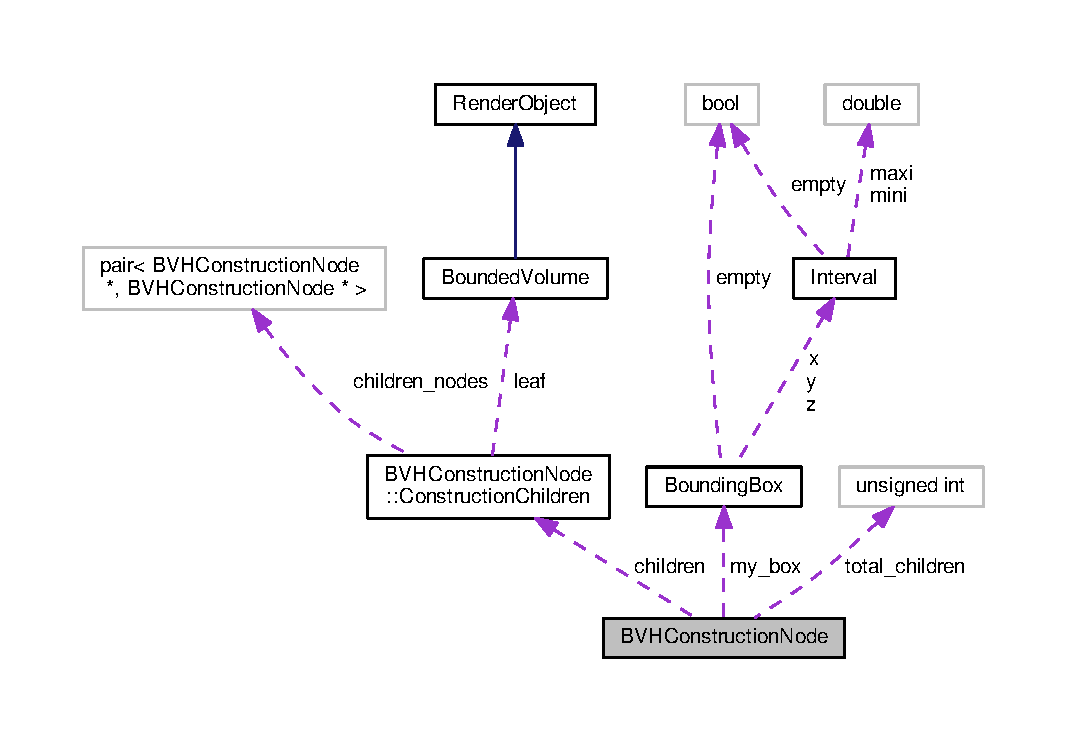
\includegraphics[width=350pt]{structBVHConstructionNode__coll__graph}
\end{center}
\end{figure}
\subsection*{Classes}
\begin{DoxyCompactItemize}
\item 
union \hyperlink{unionBVHConstructionNode_1_1ConstructionChildren}{Construction\+Children}
\end{DoxyCompactItemize}
\subsection*{Public Member Functions}
\begin{DoxyCompactItemize}
\item 
\hyperlink{structBVHConstructionNode_af28961a656f19c0a72ad44c69db2b01d}{$\sim$\+B\+V\+H\+Construction\+Node} ()
\end{DoxyCompactItemize}
\subsection*{Public Attributes}
\begin{DoxyCompactItemize}
\item 
\hyperlink{unionBVHConstructionNode_1_1ConstructionChildren}{Construction\+Children} \hyperlink{structBVHConstructionNode_a28b66929c4c6a7744f5cac8859378cf5}{children}
\item 
unsigned int \hyperlink{structBVHConstructionNode_a368f81cc16c426723f52ae5375362d54}{total\+\_\+children}
\item 
\hyperlink{classBoundingBox}{Bounding\+Box} \hyperlink{structBVHConstructionNode_a7b016f9b43b10a37c6bbb546d8289c3e}{my\+\_\+box}
\end{DoxyCompactItemize}


\subsection{Constructor \& Destructor Documentation}
\index{B\+V\+H\+Construction\+Node@{B\+V\+H\+Construction\+Node}!````~B\+V\+H\+Construction\+Node@{$\sim$\+B\+V\+H\+Construction\+Node}}
\index{````~B\+V\+H\+Construction\+Node@{$\sim$\+B\+V\+H\+Construction\+Node}!B\+V\+H\+Construction\+Node@{B\+V\+H\+Construction\+Node}}
\subsubsection[{\texorpdfstring{$\sim$\+B\+V\+H\+Construction\+Node()}{~BVHConstructionNode()}}]{\setlength{\rightskip}{0pt plus 5cm}B\+V\+H\+Construction\+Node\+::$\sim$\+B\+V\+H\+Construction\+Node (
\begin{DoxyParamCaption}
{}
\end{DoxyParamCaption}
)\hspace{0.3cm}{\ttfamily [inline]}}\hypertarget{structBVHConstructionNode_af28961a656f19c0a72ad44c69db2b01d}{}\label{structBVHConstructionNode_af28961a656f19c0a72ad44c69db2b01d}


\subsection{Member Data Documentation}
\index{B\+V\+H\+Construction\+Node@{B\+V\+H\+Construction\+Node}!children@{children}}
\index{children@{children}!B\+V\+H\+Construction\+Node@{B\+V\+H\+Construction\+Node}}
\subsubsection[{\texorpdfstring{children}{children}}]{\setlength{\rightskip}{0pt plus 5cm}{\bf Construction\+Children} B\+V\+H\+Construction\+Node\+::children}\hypertarget{structBVHConstructionNode_a28b66929c4c6a7744f5cac8859378cf5}{}\label{structBVHConstructionNode_a28b66929c4c6a7744f5cac8859378cf5}
\index{B\+V\+H\+Construction\+Node@{B\+V\+H\+Construction\+Node}!my\+\_\+box@{my\+\_\+box}}
\index{my\+\_\+box@{my\+\_\+box}!B\+V\+H\+Construction\+Node@{B\+V\+H\+Construction\+Node}}
\subsubsection[{\texorpdfstring{my\+\_\+box}{my_box}}]{\setlength{\rightskip}{0pt plus 5cm}{\bf Bounding\+Box} B\+V\+H\+Construction\+Node\+::my\+\_\+box}\hypertarget{structBVHConstructionNode_a7b016f9b43b10a37c6bbb546d8289c3e}{}\label{structBVHConstructionNode_a7b016f9b43b10a37c6bbb546d8289c3e}
\index{B\+V\+H\+Construction\+Node@{B\+V\+H\+Construction\+Node}!total\+\_\+children@{total\+\_\+children}}
\index{total\+\_\+children@{total\+\_\+children}!B\+V\+H\+Construction\+Node@{B\+V\+H\+Construction\+Node}}
\subsubsection[{\texorpdfstring{total\+\_\+children}{total_children}}]{\setlength{\rightskip}{0pt plus 5cm}unsigned int B\+V\+H\+Construction\+Node\+::total\+\_\+children}\hypertarget{structBVHConstructionNode_a368f81cc16c426723f52ae5375362d54}{}\label{structBVHConstructionNode_a368f81cc16c426723f52ae5375362d54}


The documentation for this struct was generated from the following file\+:\begin{DoxyCompactItemize}
\item 
src/renderable/\hyperlink{BinaryVolumeHierarchy_8h}{Binary\+Volume\+Hierarchy.\+h}\end{DoxyCompactItemize}

\hypertarget{structBVHLinearNode}{}\section{B\+V\+H\+Linear\+Node Struct Reference}
\label{structBVHLinearNode}\index{B\+V\+H\+Linear\+Node@{B\+V\+H\+Linear\+Node}}


{\ttfamily \#include $<$Binary\+Volume\+Hierarchy.\+h$>$}



Collaboration diagram for B\+V\+H\+Linear\+Node\+:\nopagebreak
\begin{figure}[H]
\begin{center}
\leavevmode
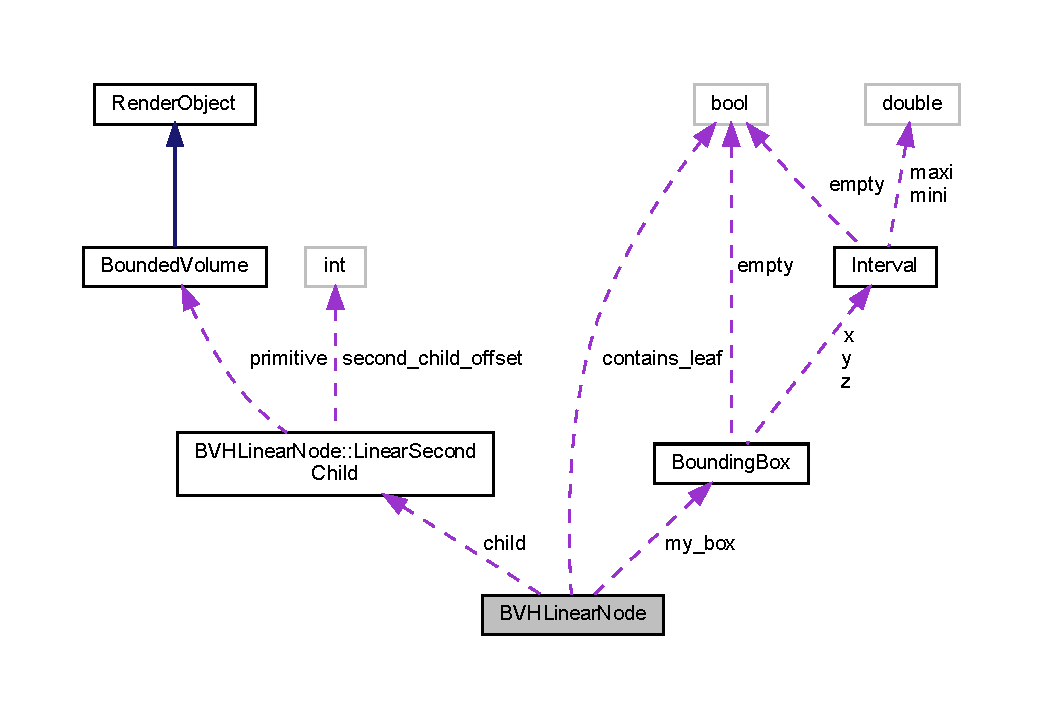
\includegraphics[width=350pt]{structBVHLinearNode__coll__graph}
\end{center}
\end{figure}
\subsection*{Classes}
\begin{DoxyCompactItemize}
\item 
union \hyperlink{unionBVHLinearNode_1_1LinearSecondChild}{Linear\+Second\+Child}
\end{DoxyCompactItemize}
\subsection*{Public Member Functions}
\begin{DoxyCompactItemize}
\item 
\hyperlink{structBVHLinearNode_ab0e9e423108e944c8c7c5ab6a35aa615}{$\sim$\+B\+V\+H\+Linear\+Node} ()=default
\end{DoxyCompactItemize}
\subsection*{Public Attributes}
\begin{DoxyCompactItemize}
\item 
\hyperlink{unionBVHLinearNode_1_1LinearSecondChild}{Linear\+Second\+Child} \hyperlink{structBVHLinearNode_a6fae5bebf63bfa365e1fab04e96e9146}{child}
\item 
\hyperlink{classBoundingBox}{Bounding\+Box} \hyperlink{structBVHLinearNode_abd02379045550966cdc50a20ea877fa5}{my\+\_\+box}
\item 
bool \hyperlink{structBVHLinearNode_aabfe3d3f0fa2893fbaa60629baea3cda}{contains\+\_\+leaf}
\end{DoxyCompactItemize}


\subsection{Constructor \& Destructor Documentation}
\index{B\+V\+H\+Linear\+Node@{B\+V\+H\+Linear\+Node}!````~B\+V\+H\+Linear\+Node@{$\sim$\+B\+V\+H\+Linear\+Node}}
\index{````~B\+V\+H\+Linear\+Node@{$\sim$\+B\+V\+H\+Linear\+Node}!B\+V\+H\+Linear\+Node@{B\+V\+H\+Linear\+Node}}
\subsubsection[{\texorpdfstring{$\sim$\+B\+V\+H\+Linear\+Node()=default}{~BVHLinearNode()=default}}]{\setlength{\rightskip}{0pt plus 5cm}B\+V\+H\+Linear\+Node\+::$\sim$\+B\+V\+H\+Linear\+Node (
\begin{DoxyParamCaption}
{}
\end{DoxyParamCaption}
)\hspace{0.3cm}{\ttfamily [default]}}\hypertarget{structBVHLinearNode_ab0e9e423108e944c8c7c5ab6a35aa615}{}\label{structBVHLinearNode_ab0e9e423108e944c8c7c5ab6a35aa615}


\subsection{Member Data Documentation}
\index{B\+V\+H\+Linear\+Node@{B\+V\+H\+Linear\+Node}!child@{child}}
\index{child@{child}!B\+V\+H\+Linear\+Node@{B\+V\+H\+Linear\+Node}}
\subsubsection[{\texorpdfstring{child}{child}}]{\setlength{\rightskip}{0pt plus 5cm}{\bf Linear\+Second\+Child} B\+V\+H\+Linear\+Node\+::child}\hypertarget{structBVHLinearNode_a6fae5bebf63bfa365e1fab04e96e9146}{}\label{structBVHLinearNode_a6fae5bebf63bfa365e1fab04e96e9146}
\index{B\+V\+H\+Linear\+Node@{B\+V\+H\+Linear\+Node}!contains\+\_\+leaf@{contains\+\_\+leaf}}
\index{contains\+\_\+leaf@{contains\+\_\+leaf}!B\+V\+H\+Linear\+Node@{B\+V\+H\+Linear\+Node}}
\subsubsection[{\texorpdfstring{contains\+\_\+leaf}{contains_leaf}}]{\setlength{\rightskip}{0pt plus 5cm}bool B\+V\+H\+Linear\+Node\+::contains\+\_\+leaf}\hypertarget{structBVHLinearNode_aabfe3d3f0fa2893fbaa60629baea3cda}{}\label{structBVHLinearNode_aabfe3d3f0fa2893fbaa60629baea3cda}
\index{B\+V\+H\+Linear\+Node@{B\+V\+H\+Linear\+Node}!my\+\_\+box@{my\+\_\+box}}
\index{my\+\_\+box@{my\+\_\+box}!B\+V\+H\+Linear\+Node@{B\+V\+H\+Linear\+Node}}
\subsubsection[{\texorpdfstring{my\+\_\+box}{my_box}}]{\setlength{\rightskip}{0pt plus 5cm}{\bf Bounding\+Box} B\+V\+H\+Linear\+Node\+::my\+\_\+box}\hypertarget{structBVHLinearNode_abd02379045550966cdc50a20ea877fa5}{}\label{structBVHLinearNode_abd02379045550966cdc50a20ea877fa5}


The documentation for this struct was generated from the following file\+:\begin{DoxyCompactItemize}
\item 
src/renderable/\hyperlink{BinaryVolumeHierarchy_8h}{Binary\+Volume\+Hierarchy.\+h}\end{DoxyCompactItemize}

\hypertarget{classcamera_1_1Camera}{}\section{camera\+:\+:Camera Class Reference}
\label{classcamera_1_1Camera}\index{camera\+::\+Camera@{camera\+::\+Camera}}


{\ttfamily \#include $<$Camera.\+h$>$}



Inheritance diagram for camera\+:\+:Camera\+:\nopagebreak
\begin{figure}[H]
\begin{center}
\leavevmode
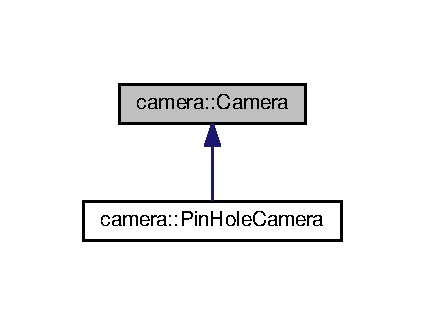
\includegraphics[width=204pt]{classcamera_1_1Camera__inherit__graph}
\end{center}
\end{figure}


Collaboration diagram for camera\+:\+:Camera\+:\nopagebreak
\begin{figure}[H]
\begin{center}
\leavevmode
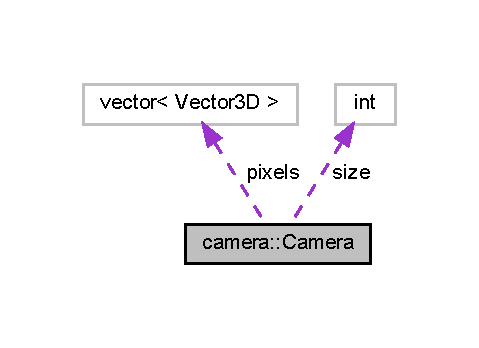
\includegraphics[width=230pt]{classcamera_1_1Camera__coll__graph}
\end{center}
\end{figure}
\subsection*{Public Member Functions}
\begin{DoxyCompactItemize}
\item 
void \hyperlink{classcamera_1_1Camera_aa6152a7c756850336a977d21a4462c6f}{set\+\_\+pixel} (unsigned int i, const \hyperlink{classVector3D}{Vector3D} \&c)
\item 
virtual \hyperlink{classRay}{Ray} \hyperlink{classcamera_1_1Camera_adf751a32f3b3b9ea5df48affafc39732}{ray\+\_\+at} (unsigned int i) const =0
\item 
void \hyperlink{classcamera_1_1Camera_a7ea257efc92d5f1d9d560ec11045e583}{write\+\_\+file} (std\+::string file\+\_\+name) const 
\item 
unsigned int \hyperlink{classcamera_1_1Camera_a423a89150b51003b1b0c75066165a980}{length} () const 
\item 
virtual \hyperlink{classcamera_1_1Camera_ae53a2162b5909211552ec49de1f5a746}{$\sim$\+Camera} ()=default
\end{DoxyCompactItemize}
\subsection*{Protected Member Functions}
\begin{DoxyCompactItemize}
\item 
virtual \hyperlink{namespacecamera_a67b7fb3d5582463a057ed122bf739b7d}{Image} \hyperlink{classcamera_1_1Camera_a56d942e3c4b51263bd7af3351da15d9f}{post\+\_\+process} () const =0
\end{DoxyCompactItemize}
\subsection*{Protected Attributes}
\begin{DoxyCompactItemize}
\item 
std\+::vector$<$ \hyperlink{classVector3D}{Vector3D} $>$ \hyperlink{classcamera_1_1Camera_a53f3fe9b838bc48e9ec21973dc8b516c}{pixels}
\item 
unsigned int \hyperlink{classcamera_1_1Camera_ac05b929c8b4f40d74ee682c4aad4c53d}{size}
\end{DoxyCompactItemize}


\subsection{Constructor \& Destructor Documentation}
\index{camera\+::\+Camera@{camera\+::\+Camera}!````~Camera@{$\sim$\+Camera}}
\index{````~Camera@{$\sim$\+Camera}!camera\+::\+Camera@{camera\+::\+Camera}}
\subsubsection[{\texorpdfstring{$\sim$\+Camera()=default}{~Camera()=default}}]{\setlength{\rightskip}{0pt plus 5cm}virtual camera\+::\+Camera\+::$\sim$\+Camera (
\begin{DoxyParamCaption}
{}
\end{DoxyParamCaption}
)\hspace{0.3cm}{\ttfamily [virtual]}, {\ttfamily [default]}}\hypertarget{classcamera_1_1Camera_ae53a2162b5909211552ec49de1f5a746}{}\label{classcamera_1_1Camera_ae53a2162b5909211552ec49de1f5a746}


\subsection{Member Function Documentation}
\index{camera\+::\+Camera@{camera\+::\+Camera}!length@{length}}
\index{length@{length}!camera\+::\+Camera@{camera\+::\+Camera}}
\subsubsection[{\texorpdfstring{length() const }{length() const }}]{\setlength{\rightskip}{0pt plus 5cm}unsigned int camera\+::\+Camera\+::length (
\begin{DoxyParamCaption}
{}
\end{DoxyParamCaption}
) const}\hypertarget{classcamera_1_1Camera_a423a89150b51003b1b0c75066165a980}{}\label{classcamera_1_1Camera_a423a89150b51003b1b0c75066165a980}
\index{camera\+::\+Camera@{camera\+::\+Camera}!post\+\_\+process@{post\+\_\+process}}
\index{post\+\_\+process@{post\+\_\+process}!camera\+::\+Camera@{camera\+::\+Camera}}
\subsubsection[{\texorpdfstring{post\+\_\+process() const =0}{post_process() const =0}}]{\setlength{\rightskip}{0pt plus 5cm}virtual {\bf Image} camera\+::\+Camera\+::post\+\_\+process (
\begin{DoxyParamCaption}
{}
\end{DoxyParamCaption}
) const\hspace{0.3cm}{\ttfamily [protected]}, {\ttfamily [pure virtual]}}\hypertarget{classcamera_1_1Camera_a56d942e3c4b51263bd7af3351da15d9f}{}\label{classcamera_1_1Camera_a56d942e3c4b51263bd7af3351da15d9f}


Implemented in \hyperlink{classcamera_1_1PinHoleCamera_a1ed550429343036f2dd14a0aacbe2c27}{camera\+::\+Pin\+Hole\+Camera}.

\index{camera\+::\+Camera@{camera\+::\+Camera}!ray\+\_\+at@{ray\+\_\+at}}
\index{ray\+\_\+at@{ray\+\_\+at}!camera\+::\+Camera@{camera\+::\+Camera}}
\subsubsection[{\texorpdfstring{ray\+\_\+at(unsigned int i) const =0}{ray_at(unsigned int i) const =0}}]{\setlength{\rightskip}{0pt plus 5cm}virtual {\bf Ray} camera\+::\+Camera\+::ray\+\_\+at (
\begin{DoxyParamCaption}
\item[{unsigned int}]{i}
\end{DoxyParamCaption}
) const\hspace{0.3cm}{\ttfamily [pure virtual]}}\hypertarget{classcamera_1_1Camera_adf751a32f3b3b9ea5df48affafc39732}{}\label{classcamera_1_1Camera_adf751a32f3b3b9ea5df48affafc39732}


Implemented in \hyperlink{classcamera_1_1PinHoleCamera_ab2457caa55561521cab10490e67ba8c8}{camera\+::\+Pin\+Hole\+Camera}.

\index{camera\+::\+Camera@{camera\+::\+Camera}!set\+\_\+pixel@{set\+\_\+pixel}}
\index{set\+\_\+pixel@{set\+\_\+pixel}!camera\+::\+Camera@{camera\+::\+Camera}}
\subsubsection[{\texorpdfstring{set\+\_\+pixel(unsigned int i, const Vector3\+D \&c)}{set_pixel(unsigned int i, const Vector3D &c)}}]{\setlength{\rightskip}{0pt plus 5cm}void camera\+::\+Camera\+::set\+\_\+pixel (
\begin{DoxyParamCaption}
\item[{unsigned int}]{i, }
\item[{const {\bf Vector3D} \&}]{c}
\end{DoxyParamCaption}
)}\hypertarget{classcamera_1_1Camera_aa6152a7c756850336a977d21a4462c6f}{}\label{classcamera_1_1Camera_aa6152a7c756850336a977d21a4462c6f}
\index{camera\+::\+Camera@{camera\+::\+Camera}!write\+\_\+file@{write\+\_\+file}}
\index{write\+\_\+file@{write\+\_\+file}!camera\+::\+Camera@{camera\+::\+Camera}}
\subsubsection[{\texorpdfstring{write\+\_\+file(std\+::string file\+\_\+name) const }{write_file(std::string file_name) const }}]{\setlength{\rightskip}{0pt plus 5cm}void camera\+::\+Camera\+::write\+\_\+file (
\begin{DoxyParamCaption}
\item[{std\+::string}]{file\+\_\+name}
\end{DoxyParamCaption}
) const}\hypertarget{classcamera_1_1Camera_a7ea257efc92d5f1d9d560ec11045e583}{}\label{classcamera_1_1Camera_a7ea257efc92d5f1d9d560ec11045e583}


\subsection{Member Data Documentation}
\index{camera\+::\+Camera@{camera\+::\+Camera}!pixels@{pixels}}
\index{pixels@{pixels}!camera\+::\+Camera@{camera\+::\+Camera}}
\subsubsection[{\texorpdfstring{pixels}{pixels}}]{\setlength{\rightskip}{0pt plus 5cm}std\+::vector$<${\bf Vector3D}$>$ camera\+::\+Camera\+::pixels\hspace{0.3cm}{\ttfamily [protected]}}\hypertarget{classcamera_1_1Camera_a53f3fe9b838bc48e9ec21973dc8b516c}{}\label{classcamera_1_1Camera_a53f3fe9b838bc48e9ec21973dc8b516c}
\index{camera\+::\+Camera@{camera\+::\+Camera}!size@{size}}
\index{size@{size}!camera\+::\+Camera@{camera\+::\+Camera}}
\subsubsection[{\texorpdfstring{size}{size}}]{\setlength{\rightskip}{0pt plus 5cm}unsigned int camera\+::\+Camera\+::size\hspace{0.3cm}{\ttfamily [protected]}}\hypertarget{classcamera_1_1Camera_ac05b929c8b4f40d74ee682c4aad4c53d}{}\label{classcamera_1_1Camera_ac05b929c8b4f40d74ee682c4aad4c53d}


The documentation for this class was generated from the following files\+:\begin{DoxyCompactItemize}
\item 
src/camera/\hyperlink{Camera_8h}{Camera.\+h}\item 
src/camera/\hyperlink{Camera_8cpp}{Camera.\+cpp}\end{DoxyCompactItemize}

\hypertarget{structsymcpp_1_1ComplexToken}{}\section{symcpp\+::Complex\+Token Struct Reference}
\label{structsymcpp_1_1ComplexToken}\index{symcpp::ComplexToken@{symcpp::ComplexToken}}


Collaboration diagram for symcpp\+::Complex\+Token\+:
\nopagebreak
\begin{figure}[H]
\begin{center}
\leavevmode
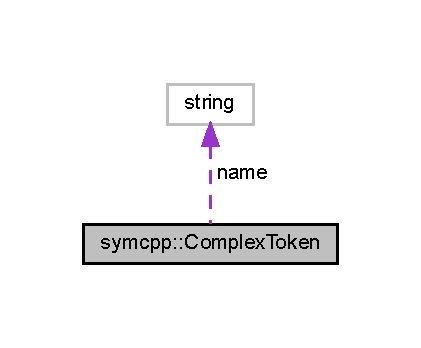
\includegraphics[width=202pt]{structsymcpp_1_1ComplexToken__coll__graph}
\end{center}
\end{figure}
\subsection*{Public Types}
\begin{DoxyCompactItemize}
\item 
enum \mbox{\hyperlink{structsymcpp_1_1ComplexToken_a5d5ae44d6f5862b7e3a409156ac54ae3}{Type}} \{ \newline
\mbox{\hyperlink{structsymcpp_1_1ComplexToken_a5d5ae44d6f5862b7e3a409156ac54ae3abd5d4f26be00a727b2a32f52b9d3d475}{V\+AR}}, 
\mbox{\hyperlink{structsymcpp_1_1ComplexToken_a5d5ae44d6f5862b7e3a409156ac54ae3a9d5179f6cc5d8de195f45da25251e202}{S\+IN}}, 
\mbox{\hyperlink{structsymcpp_1_1ComplexToken_a5d5ae44d6f5862b7e3a409156ac54ae3a3247d8325a85d40c7d15ca05421b1c5e}{C\+OS}}, 
\mbox{\hyperlink{structsymcpp_1_1ComplexToken_a5d5ae44d6f5862b7e3a409156ac54ae3aa36465d09ca3bafd575190cd520a30d8}{E\+XP}}, 
\newline
\mbox{\hyperlink{structsymcpp_1_1ComplexToken_a5d5ae44d6f5862b7e3a409156ac54ae3a2f7e0212929c29739ab0e1966aa2990a}{L\+OG}}
 \}
\end{DoxyCompactItemize}
\subsection*{Public Member Functions}
\begin{DoxyCompactItemize}
\item 
\mbox{\hyperlink{structsymcpp_1_1ComplexToken_ab67322955478ca18076d0d0d9bc985bd}{Complex\+Token}} ()
\item 
\mbox{\hyperlink{structsymcpp_1_1ComplexToken_a5d5ae44d6f5862b7e3a409156ac54ae3}{Type}} \mbox{\hyperlink{structsymcpp_1_1ComplexToken_a86c40584c46720a630fa840b5d330f63}{get\+\_\+type}} ()
\end{DoxyCompactItemize}
\subsection*{Public Attributes}
\begin{DoxyCompactItemize}
\item 
std\+::string \mbox{\hyperlink{structsymcpp_1_1ComplexToken_a0a731b7c110006afd8a1a44b400d19b4}{name}}
\end{DoxyCompactItemize}


\subsection{Member Enumeration Documentation}
\mbox{\Hypertarget{structsymcpp_1_1ComplexToken_a5d5ae44d6f5862b7e3a409156ac54ae3}\label{structsymcpp_1_1ComplexToken_a5d5ae44d6f5862b7e3a409156ac54ae3}} 
\index{symcpp::ComplexToken@{symcpp::ComplexToken}!Type@{Type}}
\index{Type@{Type}!symcpp::ComplexToken@{symcpp::ComplexToken}}
\subsubsection{\texorpdfstring{Type}{Type}}
{\footnotesize\ttfamily enum \mbox{\hyperlink{structsymcpp_1_1ComplexToken_a5d5ae44d6f5862b7e3a409156ac54ae3}{symcpp\+::\+Complex\+Token\+::\+Type}}}

\begin{DoxyEnumFields}{Enumerator}
\raisebox{\heightof{T}}[0pt][0pt]{\index{VAR@{VAR}!symcpp::ComplexToken@{symcpp::ComplexToken}}\index{symcpp::ComplexToken@{symcpp::ComplexToken}!VAR@{VAR}}}\mbox{\Hypertarget{structsymcpp_1_1ComplexToken_a5d5ae44d6f5862b7e3a409156ac54ae3abd5d4f26be00a727b2a32f52b9d3d475}\label{structsymcpp_1_1ComplexToken_a5d5ae44d6f5862b7e3a409156ac54ae3abd5d4f26be00a727b2a32f52b9d3d475}} 
V\+AR&\\
\hline

\raisebox{\heightof{T}}[0pt][0pt]{\index{SIN@{SIN}!symcpp::ComplexToken@{symcpp::ComplexToken}}\index{symcpp::ComplexToken@{symcpp::ComplexToken}!SIN@{SIN}}}\mbox{\Hypertarget{structsymcpp_1_1ComplexToken_a5d5ae44d6f5862b7e3a409156ac54ae3a9d5179f6cc5d8de195f45da25251e202}\label{structsymcpp_1_1ComplexToken_a5d5ae44d6f5862b7e3a409156ac54ae3a9d5179f6cc5d8de195f45da25251e202}} 
S\+IN&\\
\hline

\raisebox{\heightof{T}}[0pt][0pt]{\index{COS@{COS}!symcpp::ComplexToken@{symcpp::ComplexToken}}\index{symcpp::ComplexToken@{symcpp::ComplexToken}!COS@{COS}}}\mbox{\Hypertarget{structsymcpp_1_1ComplexToken_a5d5ae44d6f5862b7e3a409156ac54ae3a3247d8325a85d40c7d15ca05421b1c5e}\label{structsymcpp_1_1ComplexToken_a5d5ae44d6f5862b7e3a409156ac54ae3a3247d8325a85d40c7d15ca05421b1c5e}} 
C\+OS&\\
\hline

\raisebox{\heightof{T}}[0pt][0pt]{\index{EXP@{EXP}!symcpp::ComplexToken@{symcpp::ComplexToken}}\index{symcpp::ComplexToken@{symcpp::ComplexToken}!EXP@{EXP}}}\mbox{\Hypertarget{structsymcpp_1_1ComplexToken_a5d5ae44d6f5862b7e3a409156ac54ae3aa36465d09ca3bafd575190cd520a30d8}\label{structsymcpp_1_1ComplexToken_a5d5ae44d6f5862b7e3a409156ac54ae3aa36465d09ca3bafd575190cd520a30d8}} 
E\+XP&\\
\hline

\raisebox{\heightof{T}}[0pt][0pt]{\index{LOG@{LOG}!symcpp::ComplexToken@{symcpp::ComplexToken}}\index{symcpp::ComplexToken@{symcpp::ComplexToken}!LOG@{LOG}}}\mbox{\Hypertarget{structsymcpp_1_1ComplexToken_a5d5ae44d6f5862b7e3a409156ac54ae3a2f7e0212929c29739ab0e1966aa2990a}\label{structsymcpp_1_1ComplexToken_a5d5ae44d6f5862b7e3a409156ac54ae3a2f7e0212929c29739ab0e1966aa2990a}} 
L\+OG&\\
\hline

\end{DoxyEnumFields}


\subsection{Constructor \& Destructor Documentation}
\mbox{\Hypertarget{structsymcpp_1_1ComplexToken_ab67322955478ca18076d0d0d9bc985bd}\label{structsymcpp_1_1ComplexToken_ab67322955478ca18076d0d0d9bc985bd}} 
\index{symcpp::ComplexToken@{symcpp::ComplexToken}!ComplexToken@{ComplexToken}}
\index{ComplexToken@{ComplexToken}!symcpp::ComplexToken@{symcpp::ComplexToken}}
\subsubsection{\texorpdfstring{ComplexToken()}{ComplexToken()}}
{\footnotesize\ttfamily symcpp\+::\+Complex\+Token\+::\+Complex\+Token (\begin{DoxyParamCaption}{ }\end{DoxyParamCaption})\hspace{0.3cm}{\ttfamily [inline]}}



\subsection{Member Function Documentation}
\mbox{\Hypertarget{structsymcpp_1_1ComplexToken_a86c40584c46720a630fa840b5d330f63}\label{structsymcpp_1_1ComplexToken_a86c40584c46720a630fa840b5d330f63}} 
\index{symcpp::ComplexToken@{symcpp::ComplexToken}!get\_type@{get\_type}}
\index{get\_type@{get\_type}!symcpp::ComplexToken@{symcpp::ComplexToken}}
\subsubsection{\texorpdfstring{get\_type()}{get\_type()}}
{\footnotesize\ttfamily \mbox{\hyperlink{structsymcpp_1_1ComplexToken_a5d5ae44d6f5862b7e3a409156ac54ae3}{Type}} symcpp\+::\+Complex\+Token\+::get\+\_\+type (\begin{DoxyParamCaption}{ }\end{DoxyParamCaption})\hspace{0.3cm}{\ttfamily [inline]}}



\subsection{Member Data Documentation}
\mbox{\Hypertarget{structsymcpp_1_1ComplexToken_a0a731b7c110006afd8a1a44b400d19b4}\label{structsymcpp_1_1ComplexToken_a0a731b7c110006afd8a1a44b400d19b4}} 
\index{symcpp::ComplexToken@{symcpp::ComplexToken}!name@{name}}
\index{name@{name}!symcpp::ComplexToken@{symcpp::ComplexToken}}
\subsubsection{\texorpdfstring{name}{name}}
{\footnotesize\ttfamily std\+::string symcpp\+::\+Complex\+Token\+::name}



The documentation for this struct was generated from the following file\+:\begin{DoxyCompactItemize}
\item 
src/symcpp/\mbox{\hyperlink{SymbolicGraph_8cpp}{Symbolic\+Graph.\+cpp}}\end{DoxyCompactItemize}

\hypertarget{classsymcpp_1_1Constant}{}\section{symcpp\+:\+:Constant Class Reference}
\label{classsymcpp_1_1Constant}\index{symcpp\+::\+Constant@{symcpp\+::\+Constant}}


{\ttfamily \#include $<$Constant.\+h$>$}



Inheritance diagram for symcpp\+:\+:Constant\+:\nopagebreak
\begin{figure}[H]
\begin{center}
\leavevmode
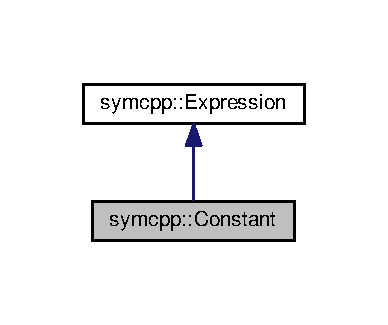
\includegraphics[width=186pt]{classsymcpp_1_1Constant__inherit__graph}
\end{center}
\end{figure}


Collaboration diagram for symcpp\+:\+:Constant\+:\nopagebreak
\begin{figure}[H]
\begin{center}
\leavevmode
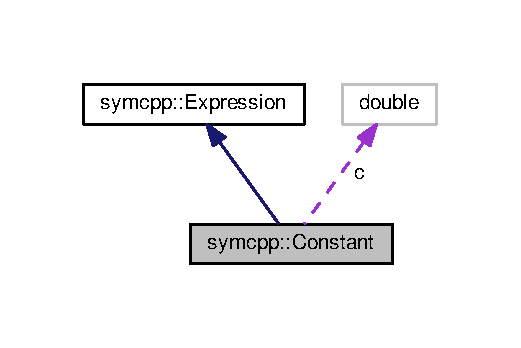
\includegraphics[width=250pt]{classsymcpp_1_1Constant__coll__graph}
\end{center}
\end{figure}
\subsection*{Public Member Functions}
\begin{DoxyCompactItemize}
\item 
\hyperlink{classsymcpp_1_1Constant_a634c91ce129b22e1b9b9afe13d4c8753}{Constant} (double \hyperlink{classsymcpp_1_1Constant_aff65de7395c014b7544c285bc131b336}{c})
\item 
std\+::unique\+\_\+ptr$<$ \hyperlink{classsymcpp_1_1Expression}{Expression} $>$ \hyperlink{classsymcpp_1_1Constant_aa5a5b0f6f06e6017ed641e8b89cd0cef}{copy} () const override
\item 
std\+::unique\+\_\+ptr$<$ \hyperlink{classsymcpp_1_1Expression}{Expression} $>$ \hyperlink{classsymcpp_1_1Constant_a19dd15712ce8630b758766e6478dec58}{diff} (std\+::string var) const override
\item 
std\+::unique\+\_\+ptr$<$ \hyperlink{classsymcpp_1_1Expression}{Expression} $>$ \hyperlink{classsymcpp_1_1Constant_a082044c6d521c2d31bbadd5db6354f96}{simplify} () override
\item 
double \hyperlink{classsymcpp_1_1Constant_ac6f62c3945429d0d318dc7d366dd4b54}{subs} (const std\+::unordered\+\_\+map$<$ std\+::string, double $>$ \&env) const override
\item 
unsigned int \hyperlink{classsymcpp_1_1Constant_a8c5e1e1b0cb2131d6f20b118f32a223f}{precedence} () const override
\item 
bool \hyperlink{classsymcpp_1_1Constant_af1ae4532a85ec5c5ed55ed8d69be68b3}{is\+\_\+constant} () const override
\item 
double \hyperlink{classsymcpp_1_1Constant_a9c2a9089ae171c2403e053a566929b45}{const\+\_\+eval} () const override
\end{DoxyCompactItemize}
\subsection*{Private Member Functions}
\begin{DoxyCompactItemize}
\item 
std\+::ostream \& \hyperlink{classsymcpp_1_1Constant_aca89e2af8df740dba562776e389edab6}{print} (std\+::ostream \&sink) const override
\end{DoxyCompactItemize}
\subsection*{Private Attributes}
\begin{DoxyCompactItemize}
\item 
double \hyperlink{classsymcpp_1_1Constant_aff65de7395c014b7544c285bc131b336}{c}
\end{DoxyCompactItemize}


\subsection{Constructor \& Destructor Documentation}
\index{symcpp\+::\+Constant@{symcpp\+::\+Constant}!Constant@{Constant}}
\index{Constant@{Constant}!symcpp\+::\+Constant@{symcpp\+::\+Constant}}
\subsubsection[{\texorpdfstring{Constant(double c)}{Constant(double c)}}]{\setlength{\rightskip}{0pt plus 5cm}symcpp\+::\+Constant\+::\+Constant (
\begin{DoxyParamCaption}
\item[{double}]{c}
\end{DoxyParamCaption}
)}\hypertarget{classsymcpp_1_1Constant_a634c91ce129b22e1b9b9afe13d4c8753}{}\label{classsymcpp_1_1Constant_a634c91ce129b22e1b9b9afe13d4c8753}


\subsection{Member Function Documentation}
\index{symcpp\+::\+Constant@{symcpp\+::\+Constant}!const\+\_\+eval@{const\+\_\+eval}}
\index{const\+\_\+eval@{const\+\_\+eval}!symcpp\+::\+Constant@{symcpp\+::\+Constant}}
\subsubsection[{\texorpdfstring{const\+\_\+eval() const override}{const_eval() const override}}]{\setlength{\rightskip}{0pt plus 5cm}double symcpp\+::\+Constant\+::const\+\_\+eval (
\begin{DoxyParamCaption}
{}
\end{DoxyParamCaption}
) const\hspace{0.3cm}{\ttfamily [override]}, {\ttfamily [virtual]}}\hypertarget{classsymcpp_1_1Constant_a9c2a9089ae171c2403e053a566929b45}{}\label{classsymcpp_1_1Constant_a9c2a9089ae171c2403e053a566929b45}


Implements \hyperlink{classsymcpp_1_1Expression_a81c8069347f586cb5632338d97c278ad}{symcpp\+::\+Expression}.

\index{symcpp\+::\+Constant@{symcpp\+::\+Constant}!copy@{copy}}
\index{copy@{copy}!symcpp\+::\+Constant@{symcpp\+::\+Constant}}
\subsubsection[{\texorpdfstring{copy() const override}{copy() const override}}]{\setlength{\rightskip}{0pt plus 5cm}std\+::unique\+\_\+ptr$<$ {\bf Expression} $>$ symcpp\+::\+Constant\+::copy (
\begin{DoxyParamCaption}
{}
\end{DoxyParamCaption}
) const\hspace{0.3cm}{\ttfamily [override]}, {\ttfamily [virtual]}}\hypertarget{classsymcpp_1_1Constant_aa5a5b0f6f06e6017ed641e8b89cd0cef}{}\label{classsymcpp_1_1Constant_aa5a5b0f6f06e6017ed641e8b89cd0cef}


Implements \hyperlink{classsymcpp_1_1Expression_a2e7de5a295ccf0efdc9b34cea7ba3d0b}{symcpp\+::\+Expression}.

\index{symcpp\+::\+Constant@{symcpp\+::\+Constant}!diff@{diff}}
\index{diff@{diff}!symcpp\+::\+Constant@{symcpp\+::\+Constant}}
\subsubsection[{\texorpdfstring{diff(std\+::string var) const override}{diff(std::string var) const override}}]{\setlength{\rightskip}{0pt plus 5cm}std\+::unique\+\_\+ptr$<$ {\bf Expression} $>$ symcpp\+::\+Constant\+::diff (
\begin{DoxyParamCaption}
\item[{std\+::string}]{var}
\end{DoxyParamCaption}
) const\hspace{0.3cm}{\ttfamily [override]}, {\ttfamily [virtual]}}\hypertarget{classsymcpp_1_1Constant_a19dd15712ce8630b758766e6478dec58}{}\label{classsymcpp_1_1Constant_a19dd15712ce8630b758766e6478dec58}


Implements \hyperlink{classsymcpp_1_1Expression_a032fe8da79d5e231ca2d21a201c8f32d}{symcpp\+::\+Expression}.

\index{symcpp\+::\+Constant@{symcpp\+::\+Constant}!is\+\_\+constant@{is\+\_\+constant}}
\index{is\+\_\+constant@{is\+\_\+constant}!symcpp\+::\+Constant@{symcpp\+::\+Constant}}
\subsubsection[{\texorpdfstring{is\+\_\+constant() const override}{is_constant() const override}}]{\setlength{\rightskip}{0pt plus 5cm}bool symcpp\+::\+Constant\+::is\+\_\+constant (
\begin{DoxyParamCaption}
{}
\end{DoxyParamCaption}
) const\hspace{0.3cm}{\ttfamily [override]}, {\ttfamily [virtual]}}\hypertarget{classsymcpp_1_1Constant_af1ae4532a85ec5c5ed55ed8d69be68b3}{}\label{classsymcpp_1_1Constant_af1ae4532a85ec5c5ed55ed8d69be68b3}


Implements \hyperlink{classsymcpp_1_1Expression_a30db7917c8948e22330cbe8259caeae2}{symcpp\+::\+Expression}.

\index{symcpp\+::\+Constant@{symcpp\+::\+Constant}!precedence@{precedence}}
\index{precedence@{precedence}!symcpp\+::\+Constant@{symcpp\+::\+Constant}}
\subsubsection[{\texorpdfstring{precedence() const override}{precedence() const override}}]{\setlength{\rightskip}{0pt plus 5cm}unsigned int symcpp\+::\+Constant\+::precedence (
\begin{DoxyParamCaption}
{}
\end{DoxyParamCaption}
) const\hspace{0.3cm}{\ttfamily [override]}, {\ttfamily [virtual]}}\hypertarget{classsymcpp_1_1Constant_a8c5e1e1b0cb2131d6f20b118f32a223f}{}\label{classsymcpp_1_1Constant_a8c5e1e1b0cb2131d6f20b118f32a223f}


Implements \hyperlink{classsymcpp_1_1Expression_a181c162d5740faac392ffdca26bfca0c}{symcpp\+::\+Expression}.

\index{symcpp\+::\+Constant@{symcpp\+::\+Constant}!print@{print}}
\index{print@{print}!symcpp\+::\+Constant@{symcpp\+::\+Constant}}
\subsubsection[{\texorpdfstring{print(std\+::ostream \&sink) const override}{print(std::ostream &sink) const override}}]{\setlength{\rightskip}{0pt plus 5cm}std\+::ostream \& symcpp\+::\+Constant\+::print (
\begin{DoxyParamCaption}
\item[{std\+::ostream \&}]{sink}
\end{DoxyParamCaption}
) const\hspace{0.3cm}{\ttfamily [override]}, {\ttfamily [private]}, {\ttfamily [virtual]}}\hypertarget{classsymcpp_1_1Constant_aca89e2af8df740dba562776e389edab6}{}\label{classsymcpp_1_1Constant_aca89e2af8df740dba562776e389edab6}


Implements \hyperlink{classsymcpp_1_1Expression_af37e13032a40f2da4d2866eaa8658049}{symcpp\+::\+Expression}.

\index{symcpp\+::\+Constant@{symcpp\+::\+Constant}!simplify@{simplify}}
\index{simplify@{simplify}!symcpp\+::\+Constant@{symcpp\+::\+Constant}}
\subsubsection[{\texorpdfstring{simplify() override}{simplify() override}}]{\setlength{\rightskip}{0pt plus 5cm}std\+::unique\+\_\+ptr$<$ {\bf Expression} $>$ symcpp\+::\+Constant\+::simplify (
\begin{DoxyParamCaption}
{}
\end{DoxyParamCaption}
)\hspace{0.3cm}{\ttfamily [override]}, {\ttfamily [virtual]}}\hypertarget{classsymcpp_1_1Constant_a082044c6d521c2d31bbadd5db6354f96}{}\label{classsymcpp_1_1Constant_a082044c6d521c2d31bbadd5db6354f96}


Implements \hyperlink{classsymcpp_1_1Expression_ab1fa6e55eea0682250d013f28db26cd2}{symcpp\+::\+Expression}.

\index{symcpp\+::\+Constant@{symcpp\+::\+Constant}!subs@{subs}}
\index{subs@{subs}!symcpp\+::\+Constant@{symcpp\+::\+Constant}}
\subsubsection[{\texorpdfstring{subs(const std\+::unordered\+\_\+map$<$ std\+::string, double $>$ \&env) const override}{subs(const std::unordered_map< std::string, double > &env) const override}}]{\setlength{\rightskip}{0pt plus 5cm}double symcpp\+::\+Constant\+::subs (
\begin{DoxyParamCaption}
\item[{const std\+::unordered\+\_\+map$<$ std\+::string, double $>$ \&}]{env}
\end{DoxyParamCaption}
) const\hspace{0.3cm}{\ttfamily [override]}, {\ttfamily [virtual]}}\hypertarget{classsymcpp_1_1Constant_ac6f62c3945429d0d318dc7d366dd4b54}{}\label{classsymcpp_1_1Constant_ac6f62c3945429d0d318dc7d366dd4b54}


Implements \hyperlink{classsymcpp_1_1Expression_aaef29b0afa2d6c21fe35f47a1be76134}{symcpp\+::\+Expression}.



\subsection{Member Data Documentation}
\index{symcpp\+::\+Constant@{symcpp\+::\+Constant}!c@{c}}
\index{c@{c}!symcpp\+::\+Constant@{symcpp\+::\+Constant}}
\subsubsection[{\texorpdfstring{c}{c}}]{\setlength{\rightskip}{0pt plus 5cm}double symcpp\+::\+Constant\+::c\hspace{0.3cm}{\ttfamily [private]}}\hypertarget{classsymcpp_1_1Constant_aff65de7395c014b7544c285bc131b336}{}\label{classsymcpp_1_1Constant_aff65de7395c014b7544c285bc131b336}


The documentation for this class was generated from the following files\+:\begin{DoxyCompactItemize}
\item 
src/symcpp/\hyperlink{Constant_8h}{Constant.\+h}\item 
src/symcpp/\hyperlink{Constant_8cpp}{Constant.\+cpp}\end{DoxyCompactItemize}

\hypertarget{unionBVHConstructionNode_1_1ConstructionChildren}{}\section{B\+V\+H\+Construction\+Node\+::Construction\+Children Union Reference}
\label{unionBVHConstructionNode_1_1ConstructionChildren}\index{BVHConstructionNode::ConstructionChildren@{BVHConstructionNode::ConstructionChildren}}


{\ttfamily \#include $<$Binary\+Volume\+Hierarchy.\+h$>$}



Collaboration diagram for B\+V\+H\+Construction\+Node\+::Construction\+Children\+:
\nopagebreak
\begin{figure}[H]
\begin{center}
\leavevmode
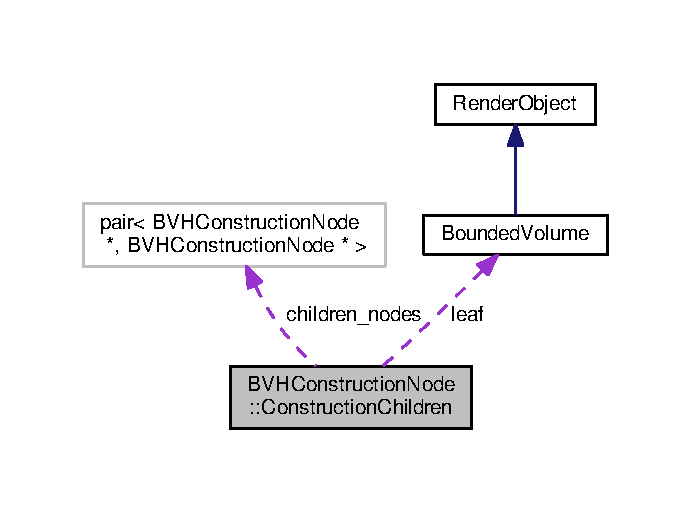
\includegraphics[width=332pt]{unionBVHConstructionNode_1_1ConstructionChildren__coll__graph}
\end{center}
\end{figure}
\subsection*{Public Attributes}
\begin{DoxyCompactItemize}
\item 
std\+::pair$<$ \mbox{\hyperlink{structBVHConstructionNode}{B\+V\+H\+Construction\+Node}} $\ast$, \mbox{\hyperlink{structBVHConstructionNode}{B\+V\+H\+Construction\+Node}} $\ast$ $>$ \mbox{\hyperlink{unionBVHConstructionNode_1_1ConstructionChildren_ac5e7d56943ed00d7165259481d7cb005}{children\+\_\+nodes}}
\item 
\mbox{\hyperlink{classBoundedVolume}{Bounded\+Volume}} $\ast$ \mbox{\hyperlink{unionBVHConstructionNode_1_1ConstructionChildren_abd717eefbb1140cd74ab66c49771b728}{leaf}}
\end{DoxyCompactItemize}


\subsection{Member Data Documentation}
\mbox{\Hypertarget{unionBVHConstructionNode_1_1ConstructionChildren_ac5e7d56943ed00d7165259481d7cb005}\label{unionBVHConstructionNode_1_1ConstructionChildren_ac5e7d56943ed00d7165259481d7cb005}} 
\index{BVHConstructionNode::ConstructionChildren@{BVHConstructionNode::ConstructionChildren}!children\_nodes@{children\_nodes}}
\index{children\_nodes@{children\_nodes}!BVHConstructionNode::ConstructionChildren@{BVHConstructionNode::ConstructionChildren}}
\subsubsection{\texorpdfstring{children\_nodes}{children\_nodes}}
{\footnotesize\ttfamily std\+::pair$<$\mbox{\hyperlink{structBVHConstructionNode}{B\+V\+H\+Construction\+Node}}$\ast$, \mbox{\hyperlink{structBVHConstructionNode}{B\+V\+H\+Construction\+Node}}$\ast$$>$ B\+V\+H\+Construction\+Node\+::\+Construction\+Children\+::children\+\_\+nodes}

\mbox{\Hypertarget{unionBVHConstructionNode_1_1ConstructionChildren_abd717eefbb1140cd74ab66c49771b728}\label{unionBVHConstructionNode_1_1ConstructionChildren_abd717eefbb1140cd74ab66c49771b728}} 
\index{BVHConstructionNode::ConstructionChildren@{BVHConstructionNode::ConstructionChildren}!leaf@{leaf}}
\index{leaf@{leaf}!BVHConstructionNode::ConstructionChildren@{BVHConstructionNode::ConstructionChildren}}
\subsubsection{\texorpdfstring{leaf}{leaf}}
{\footnotesize\ttfamily \mbox{\hyperlink{classBoundedVolume}{Bounded\+Volume}}$\ast$ B\+V\+H\+Construction\+Node\+::\+Construction\+Children\+::leaf}



The documentation for this union was generated from the following file\+:\begin{DoxyCompactItemize}
\item 
src/renderable/\mbox{\hyperlink{BinaryVolumeHierarchy_8h}{Binary\+Volume\+Hierarchy.\+h}}\end{DoxyCompactItemize}

\hypertarget{classsymcpp_1_1Cosine}{}\section{symcpp\+:\+:Cosine Class Reference}
\label{classsymcpp_1_1Cosine}\index{symcpp\+::\+Cosine@{symcpp\+::\+Cosine}}


{\ttfamily \#include $<$Cosine.\+h$>$}



Inheritance diagram for symcpp\+:\+:Cosine\+:\nopagebreak
\begin{figure}[H]
\begin{center}
\leavevmode
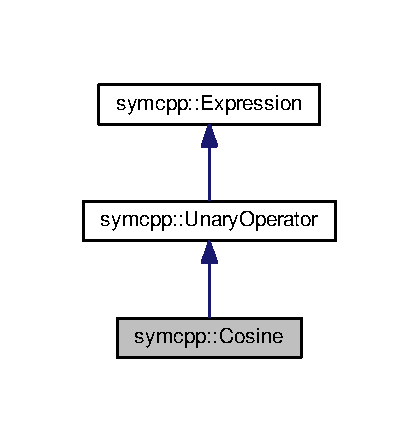
\includegraphics[width=201pt]{classsymcpp_1_1Cosine__inherit__graph}
\end{center}
\end{figure}


Collaboration diagram for symcpp\+:\+:Cosine\+:\nopagebreak
\begin{figure}[H]
\begin{center}
\leavevmode
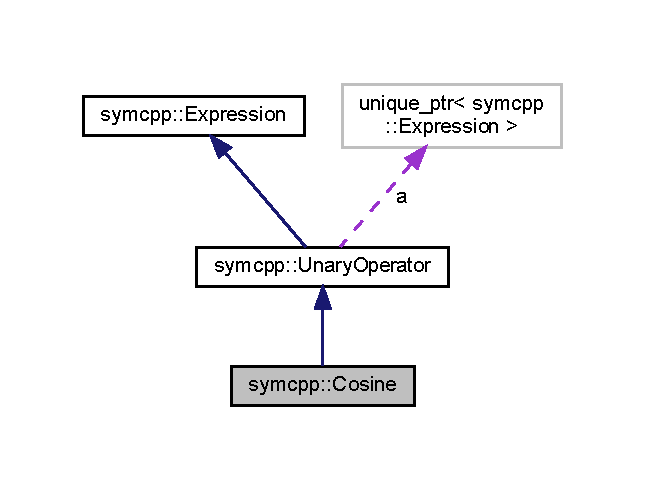
\includegraphics[width=310pt]{classsymcpp_1_1Cosine__coll__graph}
\end{center}
\end{figure}
\subsection*{Public Member Functions}
\begin{DoxyCompactItemize}
\item 
std\+::unique\+\_\+ptr$<$ \hyperlink{classsymcpp_1_1Expression}{Expression} $>$ \hyperlink{classsymcpp_1_1Cosine_a8bedd5e4ad3245d5ee6e6e7da3b5e8dc}{simplify} () override
\item 
std\+::unique\+\_\+ptr$<$ \hyperlink{classsymcpp_1_1Expression}{Expression} $>$ \hyperlink{classsymcpp_1_1Cosine_a63c4510666729dfcf5727299945c60f5}{copy} () const override
\end{DoxyCompactItemize}
\subsection*{Private Member Functions}
\begin{DoxyCompactItemize}
\item 
std\+::ostream \& \hyperlink{classsymcpp_1_1Cosine_a2d8d4dc8d5119d59365f212b7d855a53}{print} (std\+::ostream \&sink) const override
\item 
double \hyperlink{classsymcpp_1_1Cosine_a0b476eebbffe0a2914a02bf6d14b05cd}{op} (double x) const override
\item 
std\+::unique\+\_\+ptr$<$ \hyperlink{classsymcpp_1_1Expression}{Expression} $>$ \hyperlink{classsymcpp_1_1Cosine_a92a24c87300b0e400f286b6ecc4eb1dd}{partial\+\_\+derivative} () const override
\end{DoxyCompactItemize}
\subsection*{Additional Inherited Members}


\subsection{Member Function Documentation}
\index{symcpp\+::\+Cosine@{symcpp\+::\+Cosine}!copy@{copy}}
\index{copy@{copy}!symcpp\+::\+Cosine@{symcpp\+::\+Cosine}}
\subsubsection[{\texorpdfstring{copy() const override}{copy() const override}}]{\setlength{\rightskip}{0pt plus 5cm}std\+::unique\+\_\+ptr$<$ {\bf Expression} $>$ symcpp\+::\+Cosine\+::copy (
\begin{DoxyParamCaption}
{}
\end{DoxyParamCaption}
) const\hspace{0.3cm}{\ttfamily [override]}, {\ttfamily [virtual]}}\hypertarget{classsymcpp_1_1Cosine_a63c4510666729dfcf5727299945c60f5}{}\label{classsymcpp_1_1Cosine_a63c4510666729dfcf5727299945c60f5}


Implements \hyperlink{classsymcpp_1_1Expression_a2e7de5a295ccf0efdc9b34cea7ba3d0b}{symcpp\+::\+Expression}.

\index{symcpp\+::\+Cosine@{symcpp\+::\+Cosine}!op@{op}}
\index{op@{op}!symcpp\+::\+Cosine@{symcpp\+::\+Cosine}}
\subsubsection[{\texorpdfstring{op(double x) const override}{op(double x) const override}}]{\setlength{\rightskip}{0pt plus 5cm}double symcpp\+::\+Cosine\+::op (
\begin{DoxyParamCaption}
\item[{double}]{x}
\end{DoxyParamCaption}
) const\hspace{0.3cm}{\ttfamily [override]}, {\ttfamily [private]}, {\ttfamily [virtual]}}\hypertarget{classsymcpp_1_1Cosine_a0b476eebbffe0a2914a02bf6d14b05cd}{}\label{classsymcpp_1_1Cosine_a0b476eebbffe0a2914a02bf6d14b05cd}


Implements \hyperlink{classsymcpp_1_1UnaryOperator_a679c3c46cad3a62bdd776ff836c7891e}{symcpp\+::\+Unary\+Operator}.

\index{symcpp\+::\+Cosine@{symcpp\+::\+Cosine}!partial\+\_\+derivative@{partial\+\_\+derivative}}
\index{partial\+\_\+derivative@{partial\+\_\+derivative}!symcpp\+::\+Cosine@{symcpp\+::\+Cosine}}
\subsubsection[{\texorpdfstring{partial\+\_\+derivative() const override}{partial_derivative() const override}}]{\setlength{\rightskip}{0pt plus 5cm}std\+::unique\+\_\+ptr$<$ {\bf Expression} $>$ symcpp\+::\+Cosine\+::partial\+\_\+derivative (
\begin{DoxyParamCaption}
{}
\end{DoxyParamCaption}
) const\hspace{0.3cm}{\ttfamily [override]}, {\ttfamily [private]}, {\ttfamily [virtual]}}\hypertarget{classsymcpp_1_1Cosine_a92a24c87300b0e400f286b6ecc4eb1dd}{}\label{classsymcpp_1_1Cosine_a92a24c87300b0e400f286b6ecc4eb1dd}


Implements \hyperlink{classsymcpp_1_1UnaryOperator_a85de3214870cd72edc63ac1c221ddeee}{symcpp\+::\+Unary\+Operator}.

\index{symcpp\+::\+Cosine@{symcpp\+::\+Cosine}!print@{print}}
\index{print@{print}!symcpp\+::\+Cosine@{symcpp\+::\+Cosine}}
\subsubsection[{\texorpdfstring{print(std\+::ostream \&sink) const override}{print(std::ostream &sink) const override}}]{\setlength{\rightskip}{0pt plus 5cm}std\+::ostream \& symcpp\+::\+Cosine\+::print (
\begin{DoxyParamCaption}
\item[{std\+::ostream \&}]{sink}
\end{DoxyParamCaption}
) const\hspace{0.3cm}{\ttfamily [override]}, {\ttfamily [private]}, {\ttfamily [virtual]}}\hypertarget{classsymcpp_1_1Cosine_a2d8d4dc8d5119d59365f212b7d855a53}{}\label{classsymcpp_1_1Cosine_a2d8d4dc8d5119d59365f212b7d855a53}


Implements \hyperlink{classsymcpp_1_1Expression_af37e13032a40f2da4d2866eaa8658049}{symcpp\+::\+Expression}.

\index{symcpp\+::\+Cosine@{symcpp\+::\+Cosine}!simplify@{simplify}}
\index{simplify@{simplify}!symcpp\+::\+Cosine@{symcpp\+::\+Cosine}}
\subsubsection[{\texorpdfstring{simplify() override}{simplify() override}}]{\setlength{\rightskip}{0pt plus 5cm}std\+::unique\+\_\+ptr$<$ {\bf Expression} $>$ symcpp\+::\+Cosine\+::simplify (
\begin{DoxyParamCaption}
{}
\end{DoxyParamCaption}
)\hspace{0.3cm}{\ttfamily [override]}, {\ttfamily [virtual]}}\hypertarget{classsymcpp_1_1Cosine_a8bedd5e4ad3245d5ee6e6e7da3b5e8dc}{}\label{classsymcpp_1_1Cosine_a8bedd5e4ad3245d5ee6e6e7da3b5e8dc}


Implements \hyperlink{classsymcpp_1_1Expression_ab1fa6e55eea0682250d013f28db26cd2}{symcpp\+::\+Expression}.



The documentation for this class was generated from the following files\+:\begin{DoxyCompactItemize}
\item 
src/symcpp/\hyperlink{Cosine_8h}{Cosine.\+h}\item 
src/symcpp/\hyperlink{Cosine_8cpp}{Cosine.\+cpp}\end{DoxyCompactItemize}

\hypertarget{classCSG}{}\section{C\+SG Class Reference}
\label{classCSG}\index{CSG@{CSG}}


This renderable object represents a constructive solid geometry.  




{\ttfamily \#include $<$C\+S\+G.\+h$>$}



Inheritance diagram for C\+SG\+:
\nopagebreak
\begin{figure}[H]
\begin{center}
\leavevmode
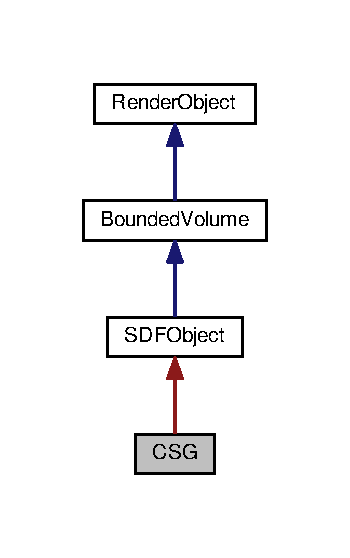
\includegraphics[width=168pt]{classCSG__inherit__graph}
\end{center}
\end{figure}


Collaboration diagram for C\+SG\+:
\nopagebreak
\begin{figure}[H]
\begin{center}
\leavevmode
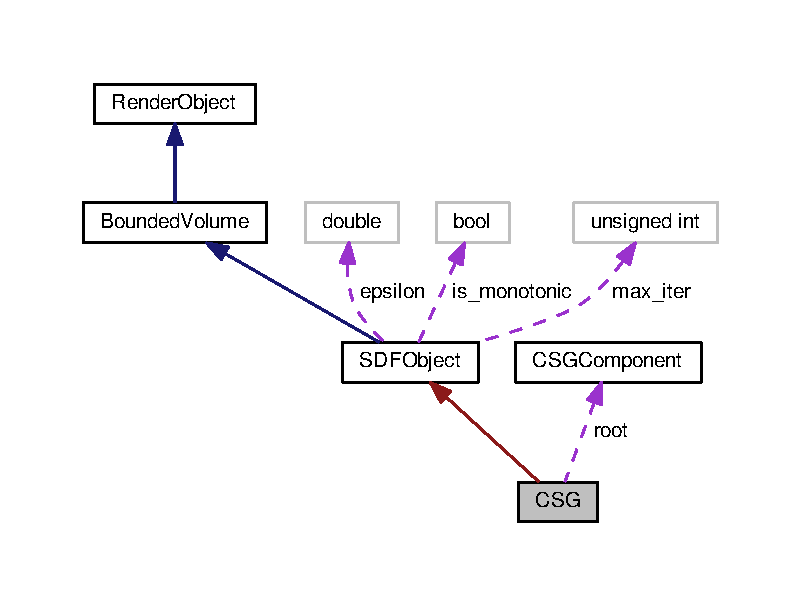
\includegraphics[width=350pt]{classCSG__coll__graph}
\end{center}
\end{figure}
\subsection*{Public Member Functions}
\begin{DoxyCompactItemize}
\item 
\mbox{\hyperlink{classCSG_a09bbc9336539ecf40021a9b3ec224afd}{C\+SG}} ()
\item 
\mbox{\hyperlink{classCSG_a9214110752f4bfead01357b5f1f7522e}{C\+SG}} (const \mbox{\hyperlink{classCSG}{C\+SG}} \&other)
\item 
\mbox{\hyperlink{classCSG}{C\+SG}} \& \mbox{\hyperlink{classCSG_a2fed963769aedb056d3f214bfe1413be}{operator=}} (const \mbox{\hyperlink{classCSG}{C\+SG}} \&other)
\item 
\mbox{\hyperlink{classCSG_a93e83c940758238fc7b188555b5a3787}{C\+SG}} (\mbox{\hyperlink{classSDFObject}{S\+D\+F\+Object}} $\ast$object)
\item 
void \mbox{\hyperlink{classCSG_a5b18efa47eb13a12633d0f5b5c1df165}{unionize}} (\mbox{\hyperlink{classSDFObject}{S\+D\+F\+Object}} $\ast$a)
\item 
void \mbox{\hyperlink{classCSG_ac44266e75a0b36097cca17e267df9873}{intersect}} (\mbox{\hyperlink{classSDFObject}{S\+D\+F\+Object}} $\ast$a)
\item 
void \mbox{\hyperlink{classCSG_a2f7550a90e950e8b143e4556b03a2a32}{subtract}} (\mbox{\hyperlink{classSDFObject}{S\+D\+F\+Object}} $\ast$a)
\item 
void \mbox{\hyperlink{classCSG_aed60985ee9a6fa106a48da72bc14582d}{unionize}} (const \mbox{\hyperlink{classCSG}{C\+SG}} \&a)
\item 
void \mbox{\hyperlink{classCSG_a1a3764a10ea7681673844ed106681569}{intersect}} (const \mbox{\hyperlink{classCSG}{C\+SG}} \&a)
\item 
void \mbox{\hyperlink{classCSG_a34a2197ec5dca9d43f88cfacbffdda53}{subtract}} (const \mbox{\hyperlink{classCSG}{C\+SG}} \&a)
\item 
\mbox{\hyperlink{classBoundingBox}{Bounding\+Box}} \mbox{\hyperlink{classCSG_abf2daf252f0b53f094ee5336eafb57ac}{get\+\_\+bounds}} () const override
\item 
\mbox{\hyperlink{classCSG_a37f03d2821dec9ee614ec6407758ba17}{$\sim$\+C\+SG}} () override
\end{DoxyCompactItemize}
\subsection*{Private Member Functions}
\begin{DoxyCompactItemize}
\item 
double \mbox{\hyperlink{classCSG_a7dc0853ae99ffd54ea99eccdc5fd5acf}{distance\+\_\+bound}} (const \mbox{\hyperlink{classVector3D}{Vector3D}} \&pos) const override
\end{DoxyCompactItemize}
\subsection*{Private Attributes}
\begin{DoxyCompactItemize}
\item 
\mbox{\hyperlink{classCSGComponent}{C\+S\+G\+Component}} $\ast$ \mbox{\hyperlink{classCSG_ae40dbc8aa97bef8f149c1b9d69e069c5}{root}}
\end{DoxyCompactItemize}


\subsection{Detailed Description}
This renderable object represents a constructive solid geometry. 

A \mbox{\hyperlink{classCSG}{C\+SG}} consists of a set of primitives, S\+D\+F\+Objects, which are composed into one object by taking their union, intersection or difference. The sequence of operations is stored as a tree, \mbox{\hyperlink{classCSG}{C\+SG}} contains a pointer to the root of this tree. Nodes in this tree implement the abstract class \mbox{\hyperlink{classCSGComponent}{C\+S\+G\+Component}}. 

\subsection{Constructor \& Destructor Documentation}
\mbox{\Hypertarget{classCSG_a09bbc9336539ecf40021a9b3ec224afd}\label{classCSG_a09bbc9336539ecf40021a9b3ec224afd}} 
\index{CSG@{CSG}!CSG@{CSG}}
\index{CSG@{CSG}!CSG@{CSG}}
\subsubsection{\texorpdfstring{CSG()}{CSG()}\hspace{0.1cm}{\footnotesize\ttfamily [1/3]}}
{\footnotesize\ttfamily C\+S\+G\+::\+C\+SG (\begin{DoxyParamCaption}{ }\end{DoxyParamCaption})}

\mbox{\Hypertarget{classCSG_a9214110752f4bfead01357b5f1f7522e}\label{classCSG_a9214110752f4bfead01357b5f1f7522e}} 
\index{CSG@{CSG}!CSG@{CSG}}
\index{CSG@{CSG}!CSG@{CSG}}
\subsubsection{\texorpdfstring{CSG()}{CSG()}\hspace{0.1cm}{\footnotesize\ttfamily [2/3]}}
{\footnotesize\ttfamily C\+S\+G\+::\+C\+SG (\begin{DoxyParamCaption}\item[{const \mbox{\hyperlink{classCSG}{C\+SG}} \&}]{other }\end{DoxyParamCaption})}

\mbox{\Hypertarget{classCSG_a93e83c940758238fc7b188555b5a3787}\label{classCSG_a93e83c940758238fc7b188555b5a3787}} 
\index{CSG@{CSG}!CSG@{CSG}}
\index{CSG@{CSG}!CSG@{CSG}}
\subsubsection{\texorpdfstring{CSG()}{CSG()}\hspace{0.1cm}{\footnotesize\ttfamily [3/3]}}
{\footnotesize\ttfamily C\+S\+G\+::\+C\+SG (\begin{DoxyParamCaption}\item[{\mbox{\hyperlink{classSDFObject}{S\+D\+F\+Object}} $\ast$}]{object }\end{DoxyParamCaption})\hspace{0.3cm}{\ttfamily [explicit]}}

\mbox{\Hypertarget{classCSG_a37f03d2821dec9ee614ec6407758ba17}\label{classCSG_a37f03d2821dec9ee614ec6407758ba17}} 
\index{CSG@{CSG}!````~CSG@{$\sim$CSG}}
\index{````~CSG@{$\sim$CSG}!CSG@{CSG}}
\subsubsection{\texorpdfstring{$\sim$CSG()}{~CSG()}}
{\footnotesize\ttfamily C\+S\+G\+::$\sim$\+C\+SG (\begin{DoxyParamCaption}{ }\end{DoxyParamCaption})\hspace{0.3cm}{\ttfamily [override]}}



\subsection{Member Function Documentation}
\mbox{\Hypertarget{classCSG_a7dc0853ae99ffd54ea99eccdc5fd5acf}\label{classCSG_a7dc0853ae99ffd54ea99eccdc5fd5acf}} 
\index{CSG@{CSG}!distance\_bound@{distance\_bound}}
\index{distance\_bound@{distance\_bound}!CSG@{CSG}}
\subsubsection{\texorpdfstring{distance\_bound()}{distance\_bound()}}
{\footnotesize\ttfamily double C\+S\+G\+::distance\+\_\+bound (\begin{DoxyParamCaption}\item[{const \mbox{\hyperlink{classVector3D}{Vector3D}} \&}]{pos }\end{DoxyParamCaption}) const\hspace{0.3cm}{\ttfamily [override]}, {\ttfamily [private]}, {\ttfamily [virtual]}}



Implements \mbox{\hyperlink{classSDFObject_ac34f5232b6ea395178d33e3b084d5a93}{S\+D\+F\+Object}}.

\mbox{\Hypertarget{classCSG_abf2daf252f0b53f094ee5336eafb57ac}\label{classCSG_abf2daf252f0b53f094ee5336eafb57ac}} 
\index{CSG@{CSG}!get\_bounds@{get\_bounds}}
\index{get\_bounds@{get\_bounds}!CSG@{CSG}}
\subsubsection{\texorpdfstring{get\_bounds()}{get\_bounds()}}
{\footnotesize\ttfamily \mbox{\hyperlink{classBoundingBox}{Bounding\+Box}} C\+S\+G\+::get\+\_\+bounds (\begin{DoxyParamCaption}{ }\end{DoxyParamCaption}) const\hspace{0.3cm}{\ttfamily [override]}, {\ttfamily [virtual]}}



Implements \mbox{\hyperlink{classBoundedVolume_a281168c4d827c38b46e639f6e4991a9e}{Bounded\+Volume}}.

\mbox{\Hypertarget{classCSG_ac44266e75a0b36097cca17e267df9873}\label{classCSG_ac44266e75a0b36097cca17e267df9873}} 
\index{CSG@{CSG}!intersect@{intersect}}
\index{intersect@{intersect}!CSG@{CSG}}
\subsubsection{\texorpdfstring{intersect()}{intersect()}\hspace{0.1cm}{\footnotesize\ttfamily [1/2]}}
{\footnotesize\ttfamily void C\+S\+G\+::intersect (\begin{DoxyParamCaption}\item[{\mbox{\hyperlink{classSDFObject}{S\+D\+F\+Object}} $\ast$}]{a }\end{DoxyParamCaption})}

\mbox{\Hypertarget{classCSG_a1a3764a10ea7681673844ed106681569}\label{classCSG_a1a3764a10ea7681673844ed106681569}} 
\index{CSG@{CSG}!intersect@{intersect}}
\index{intersect@{intersect}!CSG@{CSG}}
\subsubsection{\texorpdfstring{intersect()}{intersect()}\hspace{0.1cm}{\footnotesize\ttfamily [2/2]}}
{\footnotesize\ttfamily void C\+S\+G\+::intersect (\begin{DoxyParamCaption}\item[{const \mbox{\hyperlink{classCSG}{C\+SG}} \&}]{a }\end{DoxyParamCaption})}

\mbox{\Hypertarget{classCSG_a2fed963769aedb056d3f214bfe1413be}\label{classCSG_a2fed963769aedb056d3f214bfe1413be}} 
\index{CSG@{CSG}!operator=@{operator=}}
\index{operator=@{operator=}!CSG@{CSG}}
\subsubsection{\texorpdfstring{operator=()}{operator=()}}
{\footnotesize\ttfamily \mbox{\hyperlink{classCSG}{C\+SG}} \& C\+S\+G\+::operator= (\begin{DoxyParamCaption}\item[{const \mbox{\hyperlink{classCSG}{C\+SG}} \&}]{other }\end{DoxyParamCaption})}

\mbox{\Hypertarget{classCSG_a2f7550a90e950e8b143e4556b03a2a32}\label{classCSG_a2f7550a90e950e8b143e4556b03a2a32}} 
\index{CSG@{CSG}!subtract@{subtract}}
\index{subtract@{subtract}!CSG@{CSG}}
\subsubsection{\texorpdfstring{subtract()}{subtract()}\hspace{0.1cm}{\footnotesize\ttfamily [1/2]}}
{\footnotesize\ttfamily void C\+S\+G\+::subtract (\begin{DoxyParamCaption}\item[{\mbox{\hyperlink{classSDFObject}{S\+D\+F\+Object}} $\ast$}]{a }\end{DoxyParamCaption})}

\mbox{\Hypertarget{classCSG_a34a2197ec5dca9d43f88cfacbffdda53}\label{classCSG_a34a2197ec5dca9d43f88cfacbffdda53}} 
\index{CSG@{CSG}!subtract@{subtract}}
\index{subtract@{subtract}!CSG@{CSG}}
\subsubsection{\texorpdfstring{subtract()}{subtract()}\hspace{0.1cm}{\footnotesize\ttfamily [2/2]}}
{\footnotesize\ttfamily void C\+S\+G\+::subtract (\begin{DoxyParamCaption}\item[{const \mbox{\hyperlink{classCSG}{C\+SG}} \&}]{a }\end{DoxyParamCaption})}

\mbox{\Hypertarget{classCSG_a5b18efa47eb13a12633d0f5b5c1df165}\label{classCSG_a5b18efa47eb13a12633d0f5b5c1df165}} 
\index{CSG@{CSG}!unionize@{unionize}}
\index{unionize@{unionize}!CSG@{CSG}}
\subsubsection{\texorpdfstring{unionize()}{unionize()}\hspace{0.1cm}{\footnotesize\ttfamily [1/2]}}
{\footnotesize\ttfamily void C\+S\+G\+::unionize (\begin{DoxyParamCaption}\item[{\mbox{\hyperlink{classSDFObject}{S\+D\+F\+Object}} $\ast$}]{a }\end{DoxyParamCaption})}

\mbox{\Hypertarget{classCSG_aed60985ee9a6fa106a48da72bc14582d}\label{classCSG_aed60985ee9a6fa106a48da72bc14582d}} 
\index{CSG@{CSG}!unionize@{unionize}}
\index{unionize@{unionize}!CSG@{CSG}}
\subsubsection{\texorpdfstring{unionize()}{unionize()}\hspace{0.1cm}{\footnotesize\ttfamily [2/2]}}
{\footnotesize\ttfamily void C\+S\+G\+::unionize (\begin{DoxyParamCaption}\item[{const \mbox{\hyperlink{classCSG}{C\+SG}} \&}]{a }\end{DoxyParamCaption})}



\subsection{Member Data Documentation}
\mbox{\Hypertarget{classCSG_ae40dbc8aa97bef8f149c1b9d69e069c5}\label{classCSG_ae40dbc8aa97bef8f149c1b9d69e069c5}} 
\index{CSG@{CSG}!root@{root}}
\index{root@{root}!CSG@{CSG}}
\subsubsection{\texorpdfstring{root}{root}}
{\footnotesize\ttfamily \mbox{\hyperlink{classCSGComponent}{C\+S\+G\+Component}}$\ast$ C\+S\+G\+::root\hspace{0.3cm}{\ttfamily [private]}}



The documentation for this class was generated from the following files\+:\begin{DoxyCompactItemize}
\item 
src/renderable/\mbox{\hyperlink{CSG_8h}{C\+S\+G.\+h}}\item 
src/renderable/\mbox{\hyperlink{CSG_8cpp}{C\+S\+G.\+cpp}}\end{DoxyCompactItemize}

\hypertarget{classCSGComponent}{}\section{C\+S\+G\+Component Class Reference}
\label{classCSGComponent}\index{C\+S\+G\+Component@{C\+S\+G\+Component}}


Interface for nodes in C\+S\+G-\/\+Tree according to composition-\/pattern.  




{\ttfamily \#include $<$C\+S\+G.\+h$>$}



Inheritance diagram for C\+S\+G\+Component\+:\nopagebreak
\begin{figure}[H]
\begin{center}
\leavevmode
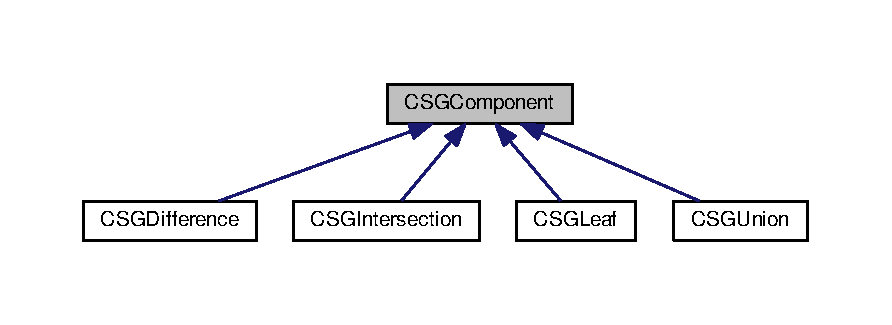
\includegraphics[width=350pt]{classCSGComponent__inherit__graph}
\end{center}
\end{figure}
\subsection*{Public Member Functions}
\begin{DoxyCompactItemize}
\item 
virtual double \hyperlink{classCSGComponent_a41ca7aff9b7c481ea076f81eeb826779}{distance\+\_\+bound} (const \hyperlink{classVector3D}{Vector3D} \&pos) const =0
\item 
virtual \hyperlink{classBoundingBox}{Bounding\+Box} \hyperlink{classCSGComponent_a4299365f2bab69272af9de4f2bee7cdb}{get\+\_\+bounds} () const =0
\item 
virtual \hyperlink{classCSGComponent}{C\+S\+G\+Component} $\ast$ \hyperlink{classCSGComponent_a98d3accd23c28259cbf490f4d7acbe83}{deep\+\_\+copy} () const =0
\item 
virtual \hyperlink{classCSGComponent_ab46aa06021795ff83ff2fdf991e5e77d}{$\sim$\+C\+S\+G\+Component} ()=default
\end{DoxyCompactItemize}


\subsection{Detailed Description}
Interface for nodes in C\+S\+G-\/\+Tree according to composition-\/pattern. 

Note, that \hyperlink{classCSGComponent}{C\+S\+G\+Component} is not renderable and is not affiliated with \hyperlink{classSDFObject}{S\+D\+F\+Object}. Although its methods have the same names, they have (formally) nothing to do with \hyperlink{classSDFObject}{S\+D\+F\+Object} or \hyperlink{classBoundingBox}{Bounding\+Box} methods. 

\subsection{Constructor \& Destructor Documentation}
\index{C\+S\+G\+Component@{C\+S\+G\+Component}!````~C\+S\+G\+Component@{$\sim$\+C\+S\+G\+Component}}
\index{````~C\+S\+G\+Component@{$\sim$\+C\+S\+G\+Component}!C\+S\+G\+Component@{C\+S\+G\+Component}}
\subsubsection[{\texorpdfstring{$\sim$\+C\+S\+G\+Component()=default}{~CSGComponent()=default}}]{\setlength{\rightskip}{0pt plus 5cm}virtual C\+S\+G\+Component\+::$\sim$\+C\+S\+G\+Component (
\begin{DoxyParamCaption}
{}
\end{DoxyParamCaption}
)\hspace{0.3cm}{\ttfamily [virtual]}, {\ttfamily [default]}}\hypertarget{classCSGComponent_ab46aa06021795ff83ff2fdf991e5e77d}{}\label{classCSGComponent_ab46aa06021795ff83ff2fdf991e5e77d}


\subsection{Member Function Documentation}
\index{C\+S\+G\+Component@{C\+S\+G\+Component}!deep\+\_\+copy@{deep\+\_\+copy}}
\index{deep\+\_\+copy@{deep\+\_\+copy}!C\+S\+G\+Component@{C\+S\+G\+Component}}
\subsubsection[{\texorpdfstring{deep\+\_\+copy() const =0}{deep_copy() const =0}}]{\setlength{\rightskip}{0pt plus 5cm}virtual {\bf C\+S\+G\+Component}$\ast$ C\+S\+G\+Component\+::deep\+\_\+copy (
\begin{DoxyParamCaption}
{}
\end{DoxyParamCaption}
) const\hspace{0.3cm}{\ttfamily [pure virtual]}}\hypertarget{classCSGComponent_a98d3accd23c28259cbf490f4d7acbe83}{}\label{classCSGComponent_a98d3accd23c28259cbf490f4d7acbe83}


Implemented in \hyperlink{classCSGLeaf_aa5142f7259d9a5d4e38797346bb6e640}{C\+S\+G\+Leaf}, \hyperlink{classCSGDifference_a8ea1d4cd7fc1ff6adca5cc4983eecfcd}{C\+S\+G\+Difference}, \hyperlink{classCSGIntersection_a4721227de85e675484ab206c299c5867}{C\+S\+G\+Intersection}, and \hyperlink{classCSGUnion_a806fa004753847d293e56a93112abe9a}{C\+S\+G\+Union}.

\index{C\+S\+G\+Component@{C\+S\+G\+Component}!distance\+\_\+bound@{distance\+\_\+bound}}
\index{distance\+\_\+bound@{distance\+\_\+bound}!C\+S\+G\+Component@{C\+S\+G\+Component}}
\subsubsection[{\texorpdfstring{distance\+\_\+bound(const Vector3\+D \&pos) const =0}{distance_bound(const Vector3D &pos) const =0}}]{\setlength{\rightskip}{0pt plus 5cm}virtual double C\+S\+G\+Component\+::distance\+\_\+bound (
\begin{DoxyParamCaption}
\item[{const {\bf Vector3D} \&}]{pos}
\end{DoxyParamCaption}
) const\hspace{0.3cm}{\ttfamily [pure virtual]}}\hypertarget{classCSGComponent_a41ca7aff9b7c481ea076f81eeb826779}{}\label{classCSGComponent_a41ca7aff9b7c481ea076f81eeb826779}


Implemented in \hyperlink{classCSGLeaf_a78d00f0c35cd87b222da10fb728037eb}{C\+S\+G\+Leaf}, \hyperlink{classCSGDifference_a66e0be492572f75b508a77c429be8fd8}{C\+S\+G\+Difference}, \hyperlink{classCSGIntersection_a199cc8192cdaeacae17d5b3c6dfef6a1}{C\+S\+G\+Intersection}, and \hyperlink{classCSGUnion_a2a15937802a57a3a78b84961fc0dda9f}{C\+S\+G\+Union}.

\index{C\+S\+G\+Component@{C\+S\+G\+Component}!get\+\_\+bounds@{get\+\_\+bounds}}
\index{get\+\_\+bounds@{get\+\_\+bounds}!C\+S\+G\+Component@{C\+S\+G\+Component}}
\subsubsection[{\texorpdfstring{get\+\_\+bounds() const =0}{get_bounds() const =0}}]{\setlength{\rightskip}{0pt plus 5cm}virtual {\bf Bounding\+Box} C\+S\+G\+Component\+::get\+\_\+bounds (
\begin{DoxyParamCaption}
{}
\end{DoxyParamCaption}
) const\hspace{0.3cm}{\ttfamily [pure virtual]}}\hypertarget{classCSGComponent_a4299365f2bab69272af9de4f2bee7cdb}{}\label{classCSGComponent_a4299365f2bab69272af9de4f2bee7cdb}


Implemented in \hyperlink{classCSGLeaf_aba3f65b725aa0a697664b9dda80b4df3}{C\+S\+G\+Leaf}, \hyperlink{classCSGDifference_aede15cd9fd46e4824e66361eb2f28ec9}{C\+S\+G\+Difference}, \hyperlink{classCSGIntersection_ad1f53a70c93dcdb6f8725a491fa24917}{C\+S\+G\+Intersection}, and \hyperlink{classCSGUnion_aaf1d2e77d8f931327fd8c499933142ba}{C\+S\+G\+Union}.



The documentation for this class was generated from the following file\+:\begin{DoxyCompactItemize}
\item 
src/renderable/\hyperlink{CSG_8h}{C\+S\+G.\+h}\end{DoxyCompactItemize}

\hypertarget{classCSGDifference}{}\section{C\+S\+G\+Difference Class Reference}
\label{classCSGDifference}\index{C\+S\+G\+Difference@{C\+S\+G\+Difference}}


A difference node in the C\+S\+G-\/\+Tree.  




{\ttfamily \#include $<$C\+S\+G.\+h$>$}



Inheritance diagram for C\+S\+G\+Difference\+:\nopagebreak
\begin{figure}[H]
\begin{center}
\leavevmode
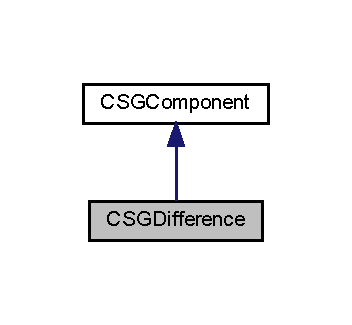
\includegraphics[width=169pt]{classCSGDifference__inherit__graph}
\end{center}
\end{figure}


Collaboration diagram for C\+S\+G\+Difference\+:\nopagebreak
\begin{figure}[H]
\begin{center}
\leavevmode
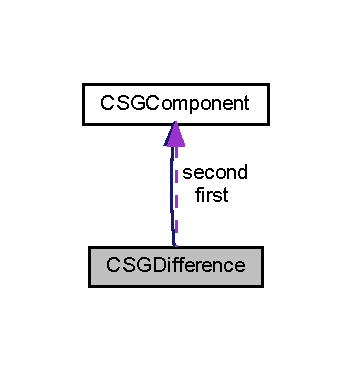
\includegraphics[width=169pt]{classCSGDifference__coll__graph}
\end{center}
\end{figure}
\subsection*{Public Member Functions}
\begin{DoxyCompactItemize}
\item 
\hyperlink{classCSGDifference_ac8012afd2f29b2546ce9b302c491fa42}{C\+S\+G\+Difference} (\hyperlink{classCSGComponent}{C\+S\+G\+Component} $\ast$a, \hyperlink{classCSGComponent}{C\+S\+G\+Component} $\ast$b)
\item 
double \hyperlink{classCSGDifference_a66e0be492572f75b508a77c429be8fd8}{distance\+\_\+bound} (const \hyperlink{classVector3D}{Vector3D} \&pos) const override
\item 
\hyperlink{classBoundingBox}{Bounding\+Box} \hyperlink{classCSGDifference_aede15cd9fd46e4824e66361eb2f28ec9}{get\+\_\+bounds} () const override
\begin{DoxyCompactList}\small\item\em Returns a \hyperlink{classBoundingBox}{Bounding\+Box} for the Difference It will simply return the \hyperlink{classBoundingBox}{Bounding\+Box} of a, this is usually a good fit. \end{DoxyCompactList}\item 
\hyperlink{classCSGComponent}{C\+S\+G\+Component} $\ast$ \hyperlink{classCSGDifference_a8ea1d4cd7fc1ff6adca5cc4983eecfcd}{deep\+\_\+copy} () const override
\item 
\hyperlink{classCSGDifference_a1f1c435a8b85ee53ee5003548e465b75}{$\sim$\+C\+S\+G\+Difference} () override
\end{DoxyCompactItemize}
\subsection*{Private Attributes}
\begin{DoxyCompactItemize}
\item 
\hyperlink{classCSGComponent}{C\+S\+G\+Component} $\ast$ \hyperlink{classCSGDifference_a689a622e9b4c43d72575cbbdd2ad847b}{first}
\item 
\hyperlink{classCSGComponent}{C\+S\+G\+Component} $\ast$ \hyperlink{classCSGDifference_ae9b4b0b0839d066ce30006d99536cd99}{second}
\end{DoxyCompactItemize}


\subsection{Detailed Description}
A difference node in the C\+S\+G-\/\+Tree. 

\subsection{Constructor \& Destructor Documentation}
\index{C\+S\+G\+Difference@{C\+S\+G\+Difference}!C\+S\+G\+Difference@{C\+S\+G\+Difference}}
\index{C\+S\+G\+Difference@{C\+S\+G\+Difference}!C\+S\+G\+Difference@{C\+S\+G\+Difference}}
\subsubsection[{\texorpdfstring{C\+S\+G\+Difference(\+C\+S\+G\+Component $\ast$a, C\+S\+G\+Component $\ast$b)}{CSGDifference(CSGComponent *a, CSGComponent *b)}}]{\setlength{\rightskip}{0pt plus 5cm}C\+S\+G\+Difference\+::\+C\+S\+G\+Difference (
\begin{DoxyParamCaption}
\item[{{\bf C\+S\+G\+Component} $\ast$}]{a, }
\item[{{\bf C\+S\+G\+Component} $\ast$}]{b}
\end{DoxyParamCaption}
)\hspace{0.3cm}{\ttfamily [inline]}}\hypertarget{classCSGDifference_ac8012afd2f29b2546ce9b302c491fa42}{}\label{classCSGDifference_ac8012afd2f29b2546ce9b302c491fa42}
\index{C\+S\+G\+Difference@{C\+S\+G\+Difference}!````~C\+S\+G\+Difference@{$\sim$\+C\+S\+G\+Difference}}
\index{````~C\+S\+G\+Difference@{$\sim$\+C\+S\+G\+Difference}!C\+S\+G\+Difference@{C\+S\+G\+Difference}}
\subsubsection[{\texorpdfstring{$\sim$\+C\+S\+G\+Difference() override}{~CSGDifference() override}}]{\setlength{\rightskip}{0pt plus 5cm}C\+S\+G\+Difference\+::$\sim$\+C\+S\+G\+Difference (
\begin{DoxyParamCaption}
{}
\end{DoxyParamCaption}
)\hspace{0.3cm}{\ttfamily [inline]}, {\ttfamily [override]}}\hypertarget{classCSGDifference_a1f1c435a8b85ee53ee5003548e465b75}{}\label{classCSGDifference_a1f1c435a8b85ee53ee5003548e465b75}


\subsection{Member Function Documentation}
\index{C\+S\+G\+Difference@{C\+S\+G\+Difference}!deep\+\_\+copy@{deep\+\_\+copy}}
\index{deep\+\_\+copy@{deep\+\_\+copy}!C\+S\+G\+Difference@{C\+S\+G\+Difference}}
\subsubsection[{\texorpdfstring{deep\+\_\+copy() const override}{deep_copy() const override}}]{\setlength{\rightskip}{0pt plus 5cm}{\bf C\+S\+G\+Component} $\ast$ C\+S\+G\+Difference\+::deep\+\_\+copy (
\begin{DoxyParamCaption}
{}
\end{DoxyParamCaption}
) const\hspace{0.3cm}{\ttfamily [override]}, {\ttfamily [virtual]}}\hypertarget{classCSGDifference_a8ea1d4cd7fc1ff6adca5cc4983eecfcd}{}\label{classCSGDifference_a8ea1d4cd7fc1ff6adca5cc4983eecfcd}


Implements \hyperlink{classCSGComponent_a98d3accd23c28259cbf490f4d7acbe83}{C\+S\+G\+Component}.

\index{C\+S\+G\+Difference@{C\+S\+G\+Difference}!distance\+\_\+bound@{distance\+\_\+bound}}
\index{distance\+\_\+bound@{distance\+\_\+bound}!C\+S\+G\+Difference@{C\+S\+G\+Difference}}
\subsubsection[{\texorpdfstring{distance\+\_\+bound(const Vector3\+D \&pos) const override}{distance_bound(const Vector3D &pos) const override}}]{\setlength{\rightskip}{0pt plus 5cm}double C\+S\+G\+Difference\+::distance\+\_\+bound (
\begin{DoxyParamCaption}
\item[{const {\bf Vector3D} \&}]{pos}
\end{DoxyParamCaption}
) const\hspace{0.3cm}{\ttfamily [override]}, {\ttfamily [virtual]}}\hypertarget{classCSGDifference_a66e0be492572f75b508a77c429be8fd8}{}\label{classCSGDifference_a66e0be492572f75b508a77c429be8fd8}


Implements \hyperlink{classCSGComponent_a41ca7aff9b7c481ea076f81eeb826779}{C\+S\+G\+Component}.

\index{C\+S\+G\+Difference@{C\+S\+G\+Difference}!get\+\_\+bounds@{get\+\_\+bounds}}
\index{get\+\_\+bounds@{get\+\_\+bounds}!C\+S\+G\+Difference@{C\+S\+G\+Difference}}
\subsubsection[{\texorpdfstring{get\+\_\+bounds() const override}{get_bounds() const override}}]{\setlength{\rightskip}{0pt plus 5cm}{\bf Bounding\+Box} C\+S\+G\+Difference\+::get\+\_\+bounds (
\begin{DoxyParamCaption}
{}
\end{DoxyParamCaption}
) const\hspace{0.3cm}{\ttfamily [override]}, {\ttfamily [virtual]}}\hypertarget{classCSGDifference_aede15cd9fd46e4824e66361eb2f28ec9}{}\label{classCSGDifference_aede15cd9fd46e4824e66361eb2f28ec9}


Returns a \hyperlink{classBoundingBox}{Bounding\+Box} for the Difference It will simply return the \hyperlink{classBoundingBox}{Bounding\+Box} of a, this is usually a good fit. 

\begin{DoxyReturn}{Returns}
\hyperlink{classBoundingBox}{Bounding\+Box} of left node 
\end{DoxyReturn}


Implements \hyperlink{classCSGComponent_a4299365f2bab69272af9de4f2bee7cdb}{C\+S\+G\+Component}.



\subsection{Member Data Documentation}
\index{C\+S\+G\+Difference@{C\+S\+G\+Difference}!first@{first}}
\index{first@{first}!C\+S\+G\+Difference@{C\+S\+G\+Difference}}
\subsubsection[{\texorpdfstring{first}{first}}]{\setlength{\rightskip}{0pt plus 5cm}{\bf C\+S\+G\+Component}$\ast$ C\+S\+G\+Difference\+::first\hspace{0.3cm}{\ttfamily [private]}}\hypertarget{classCSGDifference_a689a622e9b4c43d72575cbbdd2ad847b}{}\label{classCSGDifference_a689a622e9b4c43d72575cbbdd2ad847b}
\index{C\+S\+G\+Difference@{C\+S\+G\+Difference}!second@{second}}
\index{second@{second}!C\+S\+G\+Difference@{C\+S\+G\+Difference}}
\subsubsection[{\texorpdfstring{second}{second}}]{\setlength{\rightskip}{0pt plus 5cm}{\bf C\+S\+G\+Component}$\ast$ C\+S\+G\+Difference\+::second\hspace{0.3cm}{\ttfamily [private]}}\hypertarget{classCSGDifference_ae9b4b0b0839d066ce30006d99536cd99}{}\label{classCSGDifference_ae9b4b0b0839d066ce30006d99536cd99}


The documentation for this class was generated from the following files\+:\begin{DoxyCompactItemize}
\item 
src/renderable/\hyperlink{CSG_8h}{C\+S\+G.\+h}\item 
src/renderable/\hyperlink{CSG_8cpp}{C\+S\+G.\+cpp}\end{DoxyCompactItemize}

\hypertarget{classCSGIntersection}{}\section{C\+S\+G\+Intersection Class Reference}
\label{classCSGIntersection}\index{C\+S\+G\+Intersection@{C\+S\+G\+Intersection}}


An intersection node in the C\+S\+G-\/\+Tree.  




{\ttfamily \#include $<$C\+S\+G.\+h$>$}



Inheritance diagram for C\+S\+G\+Intersection\+:\nopagebreak
\begin{figure}[H]
\begin{center}
\leavevmode
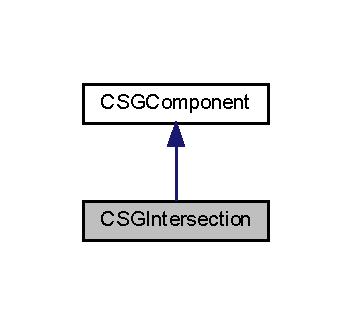
\includegraphics[width=169pt]{classCSGIntersection__inherit__graph}
\end{center}
\end{figure}


Collaboration diagram for C\+S\+G\+Intersection\+:\nopagebreak
\begin{figure}[H]
\begin{center}
\leavevmode
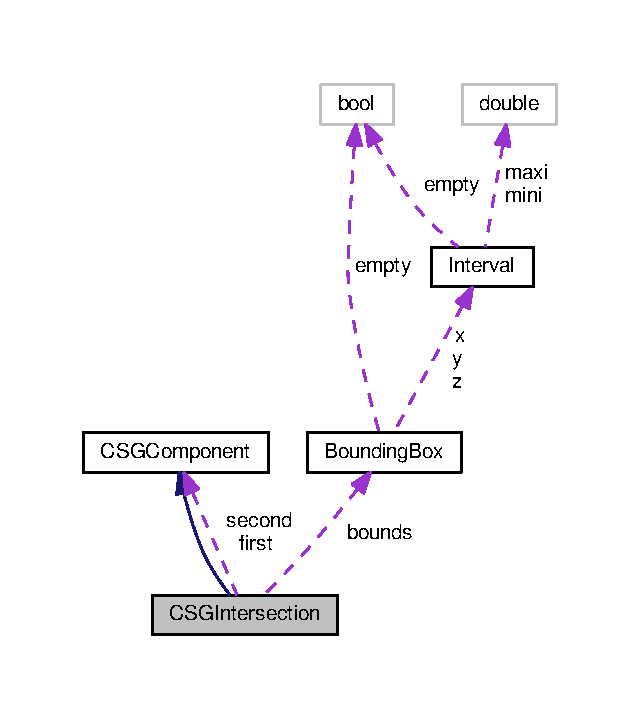
\includegraphics[width=307pt]{classCSGIntersection__coll__graph}
\end{center}
\end{figure}
\subsection*{Public Member Functions}
\begin{DoxyCompactItemize}
\item 
\hyperlink{classCSGIntersection_a0d74ea7a39a6fbfe3e6f3f918b01f63d}{C\+S\+G\+Intersection} (\hyperlink{classCSGComponent}{C\+S\+G\+Component} $\ast$a, \hyperlink{classCSGComponent}{C\+S\+G\+Component} $\ast$b)
\begin{DoxyCompactList}\small\item\em C. \end{DoxyCompactList}\item 
double \hyperlink{classCSGIntersection_a199cc8192cdaeacae17d5b3c6dfef6a1}{distance\+\_\+bound} (const \hyperlink{classVector3D}{Vector3D} \&pos) const override
\item 
\hyperlink{classBoundingBox}{Bounding\+Box} \hyperlink{classCSGIntersection_ad1f53a70c93dcdb6f8725a491fa24917}{get\+\_\+bounds} () const override
\item 
\hyperlink{classCSGComponent}{C\+S\+G\+Component} $\ast$ \hyperlink{classCSGIntersection_a4721227de85e675484ab206c299c5867}{deep\+\_\+copy} () const override
\item 
\hyperlink{classCSGIntersection_a0407d092eed23f2e6493e848482e130e}{$\sim$\+C\+S\+G\+Intersection} () override
\end{DoxyCompactItemize}
\subsection*{Private Attributes}
\begin{DoxyCompactItemize}
\item 
\hyperlink{classCSGComponent}{C\+S\+G\+Component} $\ast$ \hyperlink{classCSGIntersection_af9619c91599eb3f81342000284e0f1c6}{first}
\item 
\hyperlink{classCSGComponent}{C\+S\+G\+Component} $\ast$ \hyperlink{classCSGIntersection_a71b90fe1c487c4cc5fce0614f503e29c}{second}
\item 
\hyperlink{classBoundingBox}{Bounding\+Box} \hyperlink{classCSGIntersection_a25fb136c5dcda3e15357b6c1abb1c2e2}{bounds}
\end{DoxyCompactItemize}


\subsection{Detailed Description}
An intersection node in the C\+S\+G-\/\+Tree. 

\subsection{Constructor \& Destructor Documentation}
\index{C\+S\+G\+Intersection@{C\+S\+G\+Intersection}!C\+S\+G\+Intersection@{C\+S\+G\+Intersection}}
\index{C\+S\+G\+Intersection@{C\+S\+G\+Intersection}!C\+S\+G\+Intersection@{C\+S\+G\+Intersection}}
\subsubsection[{\texorpdfstring{C\+S\+G\+Intersection(\+C\+S\+G\+Component $\ast$a, C\+S\+G\+Component $\ast$b)}{CSGIntersection(CSGComponent *a, CSGComponent *b)}}]{\setlength{\rightskip}{0pt plus 5cm}C\+S\+G\+Intersection\+::\+C\+S\+G\+Intersection (
\begin{DoxyParamCaption}
\item[{{\bf C\+S\+G\+Component} $\ast$}]{a, }
\item[{{\bf C\+S\+G\+Component} $\ast$}]{b}
\end{DoxyParamCaption}
)\hspace{0.3cm}{\ttfamily [inline]}}\hypertarget{classCSGIntersection_a0d74ea7a39a6fbfe3e6f3f918b01f63d}{}\label{classCSGIntersection_a0d74ea7a39a6fbfe3e6f3f918b01f63d}


C. 

\index{C\+S\+G\+Intersection@{C\+S\+G\+Intersection}!````~C\+S\+G\+Intersection@{$\sim$\+C\+S\+G\+Intersection}}
\index{````~C\+S\+G\+Intersection@{$\sim$\+C\+S\+G\+Intersection}!C\+S\+G\+Intersection@{C\+S\+G\+Intersection}}
\subsubsection[{\texorpdfstring{$\sim$\+C\+S\+G\+Intersection() override}{~CSGIntersection() override}}]{\setlength{\rightskip}{0pt plus 5cm}C\+S\+G\+Intersection\+::$\sim$\+C\+S\+G\+Intersection (
\begin{DoxyParamCaption}
{}
\end{DoxyParamCaption}
)\hspace{0.3cm}{\ttfamily [inline]}, {\ttfamily [override]}}\hypertarget{classCSGIntersection_a0407d092eed23f2e6493e848482e130e}{}\label{classCSGIntersection_a0407d092eed23f2e6493e848482e130e}


\subsection{Member Function Documentation}
\index{C\+S\+G\+Intersection@{C\+S\+G\+Intersection}!deep\+\_\+copy@{deep\+\_\+copy}}
\index{deep\+\_\+copy@{deep\+\_\+copy}!C\+S\+G\+Intersection@{C\+S\+G\+Intersection}}
\subsubsection[{\texorpdfstring{deep\+\_\+copy() const override}{deep_copy() const override}}]{\setlength{\rightskip}{0pt plus 5cm}{\bf C\+S\+G\+Component} $\ast$ C\+S\+G\+Intersection\+::deep\+\_\+copy (
\begin{DoxyParamCaption}
{}
\end{DoxyParamCaption}
) const\hspace{0.3cm}{\ttfamily [override]}, {\ttfamily [virtual]}}\hypertarget{classCSGIntersection_a4721227de85e675484ab206c299c5867}{}\label{classCSGIntersection_a4721227de85e675484ab206c299c5867}


Implements \hyperlink{classCSGComponent_a98d3accd23c28259cbf490f4d7acbe83}{C\+S\+G\+Component}.

\index{C\+S\+G\+Intersection@{C\+S\+G\+Intersection}!distance\+\_\+bound@{distance\+\_\+bound}}
\index{distance\+\_\+bound@{distance\+\_\+bound}!C\+S\+G\+Intersection@{C\+S\+G\+Intersection}}
\subsubsection[{\texorpdfstring{distance\+\_\+bound(const Vector3\+D \&pos) const override}{distance_bound(const Vector3D &pos) const override}}]{\setlength{\rightskip}{0pt plus 5cm}double C\+S\+G\+Intersection\+::distance\+\_\+bound (
\begin{DoxyParamCaption}
\item[{const {\bf Vector3D} \&}]{pos}
\end{DoxyParamCaption}
) const\hspace{0.3cm}{\ttfamily [override]}, {\ttfamily [virtual]}}\hypertarget{classCSGIntersection_a199cc8192cdaeacae17d5b3c6dfef6a1}{}\label{classCSGIntersection_a199cc8192cdaeacae17d5b3c6dfef6a1}


Implements \hyperlink{classCSGComponent_a41ca7aff9b7c481ea076f81eeb826779}{C\+S\+G\+Component}.

\index{C\+S\+G\+Intersection@{C\+S\+G\+Intersection}!get\+\_\+bounds@{get\+\_\+bounds}}
\index{get\+\_\+bounds@{get\+\_\+bounds}!C\+S\+G\+Intersection@{C\+S\+G\+Intersection}}
\subsubsection[{\texorpdfstring{get\+\_\+bounds() const override}{get_bounds() const override}}]{\setlength{\rightskip}{0pt plus 5cm}{\bf Bounding\+Box} C\+S\+G\+Intersection\+::get\+\_\+bounds (
\begin{DoxyParamCaption}
{}
\end{DoxyParamCaption}
) const\hspace{0.3cm}{\ttfamily [override]}, {\ttfamily [virtual]}}\hypertarget{classCSGIntersection_ad1f53a70c93dcdb6f8725a491fa24917}{}\label{classCSGIntersection_ad1f53a70c93dcdb6f8725a491fa24917}


Implements \hyperlink{classCSGComponent_a4299365f2bab69272af9de4f2bee7cdb}{C\+S\+G\+Component}.



\subsection{Member Data Documentation}
\index{C\+S\+G\+Intersection@{C\+S\+G\+Intersection}!bounds@{bounds}}
\index{bounds@{bounds}!C\+S\+G\+Intersection@{C\+S\+G\+Intersection}}
\subsubsection[{\texorpdfstring{bounds}{bounds}}]{\setlength{\rightskip}{0pt plus 5cm}{\bf Bounding\+Box} C\+S\+G\+Intersection\+::bounds\hspace{0.3cm}{\ttfamily [private]}}\hypertarget{classCSGIntersection_a25fb136c5dcda3e15357b6c1abb1c2e2}{}\label{classCSGIntersection_a25fb136c5dcda3e15357b6c1abb1c2e2}
\index{C\+S\+G\+Intersection@{C\+S\+G\+Intersection}!first@{first}}
\index{first@{first}!C\+S\+G\+Intersection@{C\+S\+G\+Intersection}}
\subsubsection[{\texorpdfstring{first}{first}}]{\setlength{\rightskip}{0pt plus 5cm}{\bf C\+S\+G\+Component}$\ast$ C\+S\+G\+Intersection\+::first\hspace{0.3cm}{\ttfamily [private]}}\hypertarget{classCSGIntersection_af9619c91599eb3f81342000284e0f1c6}{}\label{classCSGIntersection_af9619c91599eb3f81342000284e0f1c6}
\index{C\+S\+G\+Intersection@{C\+S\+G\+Intersection}!second@{second}}
\index{second@{second}!C\+S\+G\+Intersection@{C\+S\+G\+Intersection}}
\subsubsection[{\texorpdfstring{second}{second}}]{\setlength{\rightskip}{0pt plus 5cm}{\bf C\+S\+G\+Component}$\ast$ C\+S\+G\+Intersection\+::second\hspace{0.3cm}{\ttfamily [private]}}\hypertarget{classCSGIntersection_a71b90fe1c487c4cc5fce0614f503e29c}{}\label{classCSGIntersection_a71b90fe1c487c4cc5fce0614f503e29c}


The documentation for this class was generated from the following files\+:\begin{DoxyCompactItemize}
\item 
src/renderable/\hyperlink{CSG_8h}{C\+S\+G.\+h}\item 
src/renderable/\hyperlink{CSG_8cpp}{C\+S\+G.\+cpp}\end{DoxyCompactItemize}

\hypertarget{classCSGLeaf}{}\section{C\+S\+G\+Leaf Class Reference}
\label{classCSGLeaf}\index{C\+S\+G\+Leaf@{C\+S\+G\+Leaf}}


Essentially a wrapper for Distance\+Estimated\+Object. They are leafs in the C\+S\+G-\/\+Tree.  




{\ttfamily \#include $<$C\+S\+G.\+h$>$}



Inheritance diagram for C\+S\+G\+Leaf\+:\nopagebreak
\begin{figure}[H]
\begin{center}
\leavevmode
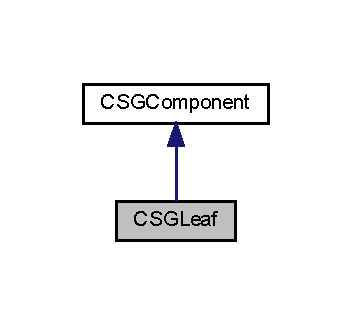
\includegraphics[width=169pt]{classCSGLeaf__inherit__graph}
\end{center}
\end{figure}


Collaboration diagram for C\+S\+G\+Leaf\+:
\nopagebreak
\begin{figure}[H]
\begin{center}
\leavevmode
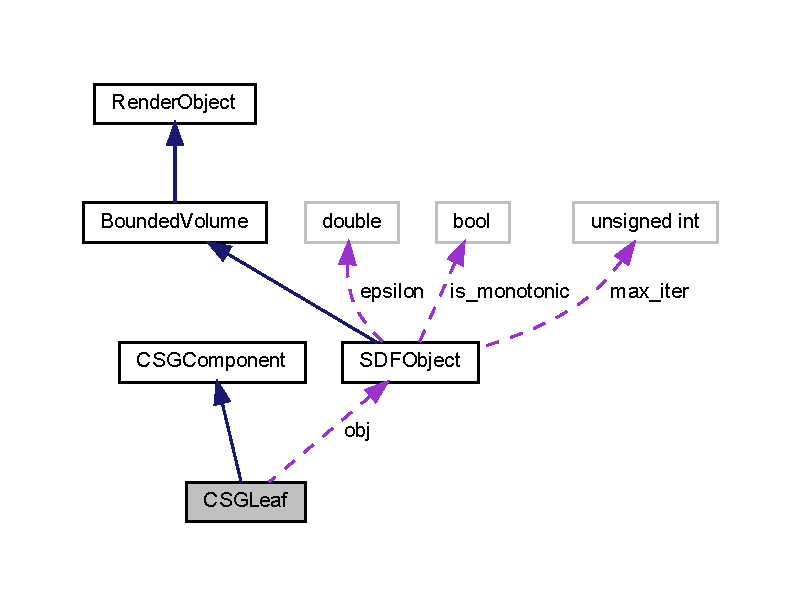
\includegraphics[width=350pt]{classCSGLeaf__coll__graph}
\end{center}
\end{figure}
\subsection*{Public Member Functions}
\begin{DoxyCompactItemize}
\item 
\hyperlink{classCSGLeaf_ac0843162c744c30a1ea0a97ec41e6c72}{C\+S\+G\+Leaf} (\hyperlink{classSDFObject}{S\+D\+F\+Object} $\ast$a)
\item 
double \hyperlink{classCSGLeaf_a78d00f0c35cd87b222da10fb728037eb}{distance\+\_\+bound} (const \hyperlink{classVector3D}{Vector3D} \&pos) const override
\item 
\hyperlink{classBoundingBox}{Bounding\+Box} \hyperlink{classCSGLeaf_aba3f65b725aa0a697664b9dda80b4df3}{get\+\_\+bounds} () const override
\item 
\hyperlink{classCSGComponent}{C\+S\+G\+Component} $\ast$ \hyperlink{classCSGLeaf_aa5142f7259d9a5d4e38797346bb6e640}{deep\+\_\+copy} () const override
\item 
\hyperlink{classCSGLeaf_ae6814ea82f8bdaa79eb0c98f25d6334b}{$\sim$\+C\+S\+G\+Leaf} () override=default
\end{DoxyCompactItemize}
\subsection*{Private Attributes}
\begin{DoxyCompactItemize}
\item 
\hyperlink{classSDFObject}{S\+D\+F\+Object} $\ast$ \hyperlink{classCSGLeaf_a6bb40cb3c028d643273d5da84f01e4b0}{obj}
\end{DoxyCompactItemize}


\subsection{Detailed Description}
Essentially a wrapper for Distance\+Estimated\+Object. They are leafs in the C\+S\+G-\/\+Tree. 

\subsection{Constructor \& Destructor Documentation}
\index{C\+S\+G\+Leaf@{C\+S\+G\+Leaf}!C\+S\+G\+Leaf@{C\+S\+G\+Leaf}}
\index{C\+S\+G\+Leaf@{C\+S\+G\+Leaf}!C\+S\+G\+Leaf@{C\+S\+G\+Leaf}}
\subsubsection[{\texorpdfstring{C\+S\+G\+Leaf(\+S\+D\+F\+Object $\ast$a)}{CSGLeaf(SDFObject *a)}}]{\setlength{\rightskip}{0pt plus 5cm}C\+S\+G\+Leaf\+::\+C\+S\+G\+Leaf (
\begin{DoxyParamCaption}
\item[{{\bf S\+D\+F\+Object} $\ast$}]{a}
\end{DoxyParamCaption}
)\hspace{0.3cm}{\ttfamily [inline]}, {\ttfamily [explicit]}}\hypertarget{classCSGLeaf_ac0843162c744c30a1ea0a97ec41e6c72}{}\label{classCSGLeaf_ac0843162c744c30a1ea0a97ec41e6c72}
\index{C\+S\+G\+Leaf@{C\+S\+G\+Leaf}!````~C\+S\+G\+Leaf@{$\sim$\+C\+S\+G\+Leaf}}
\index{````~C\+S\+G\+Leaf@{$\sim$\+C\+S\+G\+Leaf}!C\+S\+G\+Leaf@{C\+S\+G\+Leaf}}
\subsubsection[{\texorpdfstring{$\sim$\+C\+S\+G\+Leaf() override=default}{~CSGLeaf() override=default}}]{\setlength{\rightskip}{0pt plus 5cm}C\+S\+G\+Leaf\+::$\sim$\+C\+S\+G\+Leaf (
\begin{DoxyParamCaption}
{}
\end{DoxyParamCaption}
)\hspace{0.3cm}{\ttfamily [override]}, {\ttfamily [default]}}\hypertarget{classCSGLeaf_ae6814ea82f8bdaa79eb0c98f25d6334b}{}\label{classCSGLeaf_ae6814ea82f8bdaa79eb0c98f25d6334b}


\subsection{Member Function Documentation}
\index{C\+S\+G\+Leaf@{C\+S\+G\+Leaf}!deep\+\_\+copy@{deep\+\_\+copy}}
\index{deep\+\_\+copy@{deep\+\_\+copy}!C\+S\+G\+Leaf@{C\+S\+G\+Leaf}}
\subsubsection[{\texorpdfstring{deep\+\_\+copy() const override}{deep_copy() const override}}]{\setlength{\rightskip}{0pt plus 5cm}{\bf C\+S\+G\+Component} $\ast$ C\+S\+G\+Leaf\+::deep\+\_\+copy (
\begin{DoxyParamCaption}
{}
\end{DoxyParamCaption}
) const\hspace{0.3cm}{\ttfamily [override]}, {\ttfamily [virtual]}}\hypertarget{classCSGLeaf_aa5142f7259d9a5d4e38797346bb6e640}{}\label{classCSGLeaf_aa5142f7259d9a5d4e38797346bb6e640}


Implements \hyperlink{classCSGComponent_a98d3accd23c28259cbf490f4d7acbe83}{C\+S\+G\+Component}.

\index{C\+S\+G\+Leaf@{C\+S\+G\+Leaf}!distance\+\_\+bound@{distance\+\_\+bound}}
\index{distance\+\_\+bound@{distance\+\_\+bound}!C\+S\+G\+Leaf@{C\+S\+G\+Leaf}}
\subsubsection[{\texorpdfstring{distance\+\_\+bound(const Vector3\+D \&pos) const override}{distance_bound(const Vector3D &pos) const override}}]{\setlength{\rightskip}{0pt plus 5cm}double C\+S\+G\+Leaf\+::distance\+\_\+bound (
\begin{DoxyParamCaption}
\item[{const {\bf Vector3D} \&}]{pos}
\end{DoxyParamCaption}
) const\hspace{0.3cm}{\ttfamily [inline]}, {\ttfamily [override]}, {\ttfamily [virtual]}}\hypertarget{classCSGLeaf_a78d00f0c35cd87b222da10fb728037eb}{}\label{classCSGLeaf_a78d00f0c35cd87b222da10fb728037eb}


Implements \hyperlink{classCSGComponent_a41ca7aff9b7c481ea076f81eeb826779}{C\+S\+G\+Component}.

\index{C\+S\+G\+Leaf@{C\+S\+G\+Leaf}!get\+\_\+bounds@{get\+\_\+bounds}}
\index{get\+\_\+bounds@{get\+\_\+bounds}!C\+S\+G\+Leaf@{C\+S\+G\+Leaf}}
\subsubsection[{\texorpdfstring{get\+\_\+bounds() const override}{get_bounds() const override}}]{\setlength{\rightskip}{0pt plus 5cm}{\bf Bounding\+Box} C\+S\+G\+Leaf\+::get\+\_\+bounds (
\begin{DoxyParamCaption}
{}
\end{DoxyParamCaption}
) const\hspace{0.3cm}{\ttfamily [override]}, {\ttfamily [virtual]}}\hypertarget{classCSGLeaf_aba3f65b725aa0a697664b9dda80b4df3}{}\label{classCSGLeaf_aba3f65b725aa0a697664b9dda80b4df3}


Implements \hyperlink{classCSGComponent_a4299365f2bab69272af9de4f2bee7cdb}{C\+S\+G\+Component}.



\subsection{Member Data Documentation}
\index{C\+S\+G\+Leaf@{C\+S\+G\+Leaf}!obj@{obj}}
\index{obj@{obj}!C\+S\+G\+Leaf@{C\+S\+G\+Leaf}}
\subsubsection[{\texorpdfstring{obj}{obj}}]{\setlength{\rightskip}{0pt plus 5cm}{\bf S\+D\+F\+Object}$\ast$ C\+S\+G\+Leaf\+::obj\hspace{0.3cm}{\ttfamily [private]}}\hypertarget{classCSGLeaf_a6bb40cb3c028d643273d5da84f01e4b0}{}\label{classCSGLeaf_a6bb40cb3c028d643273d5da84f01e4b0}


The documentation for this class was generated from the following files\+:\begin{DoxyCompactItemize}
\item 
src/renderable/\hyperlink{CSG_8h}{C\+S\+G.\+h}\item 
src/renderable/\hyperlink{CSG_8cpp}{C\+S\+G.\+cpp}\end{DoxyCompactItemize}

\hypertarget{classCSGUnion}{}\section{C\+S\+G\+Union Class Reference}
\label{classCSGUnion}\index{C\+S\+G\+Union@{C\+S\+G\+Union}}


A union node in the C\+S\+G-\/\+Tree.  




{\ttfamily \#include $<$C\+S\+G.\+h$>$}



Inheritance diagram for C\+S\+G\+Union\+:\nopagebreak
\begin{figure}[H]
\begin{center}
\leavevmode
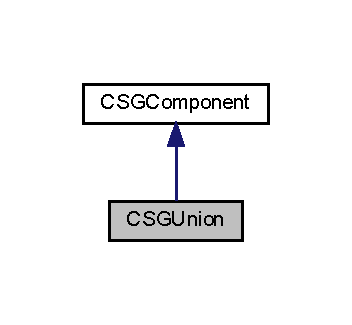
\includegraphics[width=169pt]{classCSGUnion__inherit__graph}
\end{center}
\end{figure}


Collaboration diagram for C\+S\+G\+Union\+:\nopagebreak
\begin{figure}[H]
\begin{center}
\leavevmode
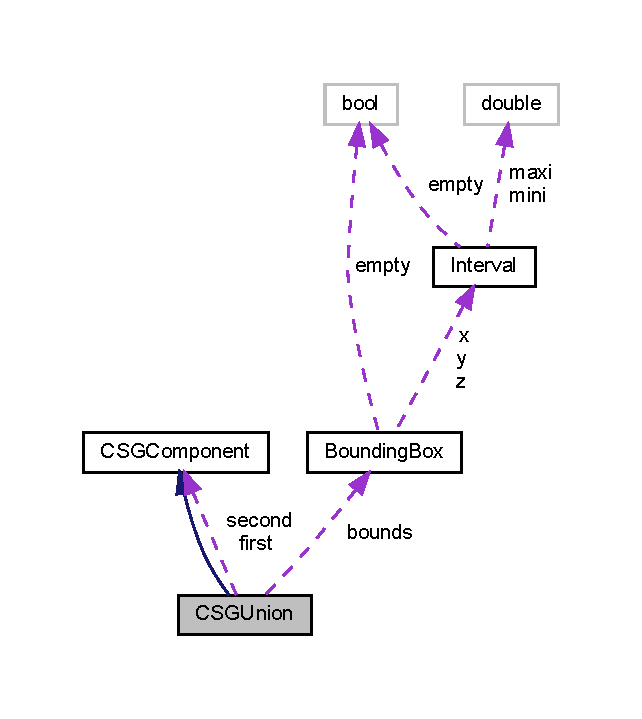
\includegraphics[width=307pt]{classCSGUnion__coll__graph}
\end{center}
\end{figure}
\subsection*{Public Member Functions}
\begin{DoxyCompactItemize}
\item 
\hyperlink{classCSGUnion_a89f33aab1b6e073a2813f97cc3998fc7}{C\+S\+G\+Union} (\hyperlink{classCSGComponent}{C\+S\+G\+Component} $\ast$a, \hyperlink{classCSGComponent}{C\+S\+G\+Component} $\ast$b)
\begin{DoxyCompactList}\small\item\em Create a Union-\/\+Node for a C\+S\+G-\/\+Tree. \end{DoxyCompactList}\item 
double \hyperlink{classCSGUnion_a2a15937802a57a3a78b84961fc0dda9f}{distance\+\_\+bound} (const \hyperlink{classVector3D}{Vector3D} \&pos) const override
\item 
\hyperlink{classBoundingBox}{Bounding\+Box} \hyperlink{classCSGUnion_aaf1d2e77d8f931327fd8c499933142ba}{get\+\_\+bounds} () const override
\item 
\hyperlink{classCSGComponent}{C\+S\+G\+Component} $\ast$ \hyperlink{classCSGUnion_a806fa004753847d293e56a93112abe9a}{deep\+\_\+copy} () const override
\item 
\hyperlink{classCSGUnion_af16ab807f0e1140de88007a5606f2a91}{$\sim$\+C\+S\+G\+Union} () override
\end{DoxyCompactItemize}
\subsection*{Private Attributes}
\begin{DoxyCompactItemize}
\item 
\hyperlink{classCSGComponent}{C\+S\+G\+Component} $\ast$ \hyperlink{classCSGUnion_ac2042150362043f8646dc9f13e98df1a}{first}
\item 
\hyperlink{classCSGComponent}{C\+S\+G\+Component} $\ast$ \hyperlink{classCSGUnion_abb2099a585c204bdcf3c2d0c8004438e}{second}
\item 
\hyperlink{classBoundingBox}{Bounding\+Box} \hyperlink{classCSGUnion_a40b5e5f99930721873da62db801e0c90}{bounds}
\end{DoxyCompactItemize}


\subsection{Detailed Description}
A union node in the C\+S\+G-\/\+Tree. 

\subsection{Constructor \& Destructor Documentation}
\index{C\+S\+G\+Union@{C\+S\+G\+Union}!C\+S\+G\+Union@{C\+S\+G\+Union}}
\index{C\+S\+G\+Union@{C\+S\+G\+Union}!C\+S\+G\+Union@{C\+S\+G\+Union}}
\subsubsection[{\texorpdfstring{C\+S\+G\+Union(\+C\+S\+G\+Component $\ast$a, C\+S\+G\+Component $\ast$b)}{CSGUnion(CSGComponent *a, CSGComponent *b)}}]{\setlength{\rightskip}{0pt plus 5cm}C\+S\+G\+Union\+::\+C\+S\+G\+Union (
\begin{DoxyParamCaption}
\item[{{\bf C\+S\+G\+Component} $\ast$}]{a, }
\item[{{\bf C\+S\+G\+Component} $\ast$}]{b}
\end{DoxyParamCaption}
)\hspace{0.3cm}{\ttfamily [inline]}}\hypertarget{classCSGUnion_a89f33aab1b6e073a2813f97cc3998fc7}{}\label{classCSGUnion_a89f33aab1b6e073a2813f97cc3998fc7}


Create a Union-\/\+Node for a C\+S\+G-\/\+Tree. 


\begin{DoxyParams}{Parameters}
{\em a} & The first node \\
\hline
{\em b} & The second \\
\hline
\end{DoxyParams}
\index{C\+S\+G\+Union@{C\+S\+G\+Union}!````~C\+S\+G\+Union@{$\sim$\+C\+S\+G\+Union}}
\index{````~C\+S\+G\+Union@{$\sim$\+C\+S\+G\+Union}!C\+S\+G\+Union@{C\+S\+G\+Union}}
\subsubsection[{\texorpdfstring{$\sim$\+C\+S\+G\+Union() override}{~CSGUnion() override}}]{\setlength{\rightskip}{0pt plus 5cm}C\+S\+G\+Union\+::$\sim$\+C\+S\+G\+Union (
\begin{DoxyParamCaption}
{}
\end{DoxyParamCaption}
)\hspace{0.3cm}{\ttfamily [inline]}, {\ttfamily [override]}}\hypertarget{classCSGUnion_af16ab807f0e1140de88007a5606f2a91}{}\label{classCSGUnion_af16ab807f0e1140de88007a5606f2a91}


\subsection{Member Function Documentation}
\index{C\+S\+G\+Union@{C\+S\+G\+Union}!deep\+\_\+copy@{deep\+\_\+copy}}
\index{deep\+\_\+copy@{deep\+\_\+copy}!C\+S\+G\+Union@{C\+S\+G\+Union}}
\subsubsection[{\texorpdfstring{deep\+\_\+copy() const override}{deep_copy() const override}}]{\setlength{\rightskip}{0pt plus 5cm}{\bf C\+S\+G\+Component} $\ast$ C\+S\+G\+Union\+::deep\+\_\+copy (
\begin{DoxyParamCaption}
{}
\end{DoxyParamCaption}
) const\hspace{0.3cm}{\ttfamily [override]}, {\ttfamily [virtual]}}\hypertarget{classCSGUnion_a806fa004753847d293e56a93112abe9a}{}\label{classCSGUnion_a806fa004753847d293e56a93112abe9a}


Implements \hyperlink{classCSGComponent_a98d3accd23c28259cbf490f4d7acbe83}{C\+S\+G\+Component}.

\index{C\+S\+G\+Union@{C\+S\+G\+Union}!distance\+\_\+bound@{distance\+\_\+bound}}
\index{distance\+\_\+bound@{distance\+\_\+bound}!C\+S\+G\+Union@{C\+S\+G\+Union}}
\subsubsection[{\texorpdfstring{distance\+\_\+bound(const Vector3\+D \&pos) const override}{distance_bound(const Vector3D &pos) const override}}]{\setlength{\rightskip}{0pt plus 5cm}double C\+S\+G\+Union\+::distance\+\_\+bound (
\begin{DoxyParamCaption}
\item[{const {\bf Vector3D} \&}]{pos}
\end{DoxyParamCaption}
) const\hspace{0.3cm}{\ttfamily [override]}, {\ttfamily [virtual]}}\hypertarget{classCSGUnion_a2a15937802a57a3a78b84961fc0dda9f}{}\label{classCSGUnion_a2a15937802a57a3a78b84961fc0dda9f}


Implements \hyperlink{classCSGComponent_a41ca7aff9b7c481ea076f81eeb826779}{C\+S\+G\+Component}.

\index{C\+S\+G\+Union@{C\+S\+G\+Union}!get\+\_\+bounds@{get\+\_\+bounds}}
\index{get\+\_\+bounds@{get\+\_\+bounds}!C\+S\+G\+Union@{C\+S\+G\+Union}}
\subsubsection[{\texorpdfstring{get\+\_\+bounds() const override}{get_bounds() const override}}]{\setlength{\rightskip}{0pt plus 5cm}{\bf Bounding\+Box} C\+S\+G\+Union\+::get\+\_\+bounds (
\begin{DoxyParamCaption}
{}
\end{DoxyParamCaption}
) const\hspace{0.3cm}{\ttfamily [override]}, {\ttfamily [virtual]}}\hypertarget{classCSGUnion_aaf1d2e77d8f931327fd8c499933142ba}{}\label{classCSGUnion_aaf1d2e77d8f931327fd8c499933142ba}


Implements \hyperlink{classCSGComponent_a4299365f2bab69272af9de4f2bee7cdb}{C\+S\+G\+Component}.



\subsection{Member Data Documentation}
\index{C\+S\+G\+Union@{C\+S\+G\+Union}!bounds@{bounds}}
\index{bounds@{bounds}!C\+S\+G\+Union@{C\+S\+G\+Union}}
\subsubsection[{\texorpdfstring{bounds}{bounds}}]{\setlength{\rightskip}{0pt plus 5cm}{\bf Bounding\+Box} C\+S\+G\+Union\+::bounds\hspace{0.3cm}{\ttfamily [private]}}\hypertarget{classCSGUnion_a40b5e5f99930721873da62db801e0c90}{}\label{classCSGUnion_a40b5e5f99930721873da62db801e0c90}
\index{C\+S\+G\+Union@{C\+S\+G\+Union}!first@{first}}
\index{first@{first}!C\+S\+G\+Union@{C\+S\+G\+Union}}
\subsubsection[{\texorpdfstring{first}{first}}]{\setlength{\rightskip}{0pt plus 5cm}{\bf C\+S\+G\+Component}$\ast$ C\+S\+G\+Union\+::first\hspace{0.3cm}{\ttfamily [private]}}\hypertarget{classCSGUnion_ac2042150362043f8646dc9f13e98df1a}{}\label{classCSGUnion_ac2042150362043f8646dc9f13e98df1a}
\index{C\+S\+G\+Union@{C\+S\+G\+Union}!second@{second}}
\index{second@{second}!C\+S\+G\+Union@{C\+S\+G\+Union}}
\subsubsection[{\texorpdfstring{second}{second}}]{\setlength{\rightskip}{0pt plus 5cm}{\bf C\+S\+G\+Component}$\ast$ C\+S\+G\+Union\+::second\hspace{0.3cm}{\ttfamily [private]}}\hypertarget{classCSGUnion_abb2099a585c204bdcf3c2d0c8004438e}{}\label{classCSGUnion_abb2099a585c204bdcf3c2d0c8004438e}


The documentation for this class was generated from the following files\+:\begin{DoxyCompactItemize}
\item 
src/renderable/\hyperlink{CSG_8h}{C\+S\+G.\+h}\item 
src/renderable/\hyperlink{CSG_8cpp}{C\+S\+G.\+cpp}\end{DoxyCompactItemize}

\hypertarget{classDistantPointSource}{}\section{Distant\+Point\+Source Class Reference}
\label{classDistantPointSource}\index{Distant\+Point\+Source@{Distant\+Point\+Source}}


{\ttfamily \#include $<$Distant\+Point\+Source.\+h$>$}



Inheritance diagram for Distant\+Point\+Source\+:\nopagebreak
\begin{figure}[H]
\begin{center}
\leavevmode
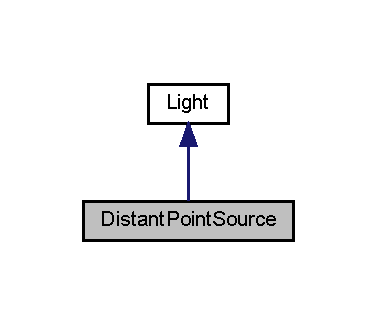
\includegraphics[width=181pt]{classDistantPointSource__inherit__graph}
\end{center}
\end{figure}


Collaboration diagram for Distant\+Point\+Source\+:\nopagebreak
\begin{figure}[H]
\begin{center}
\leavevmode
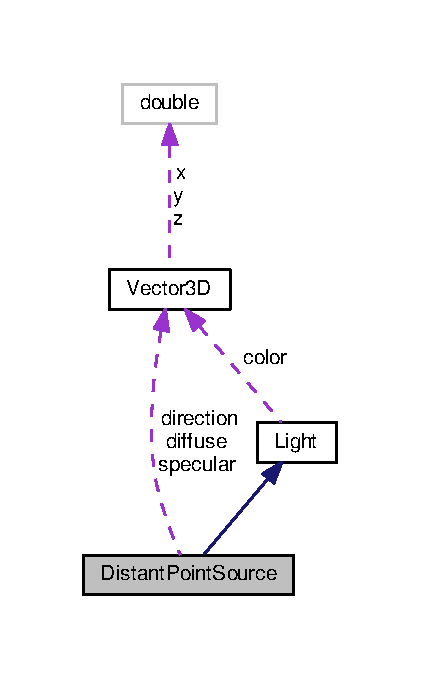
\includegraphics[width=202pt]{classDistantPointSource__coll__graph}
\end{center}
\end{figure}
\subsection*{Public Member Functions}
\begin{DoxyCompactItemize}
\item 
\hyperlink{classDistantPointSource_abb36a1b1376c1d895e11ba5a01466a0b}{Distant\+Point\+Source} (\hyperlink{classVector3D}{Vector3D} dir, \hyperlink{classVector3D}{Vector3D} \hyperlink{classDistantPointSource_af6bebc971d66f68f97045712db771411}{specular}, \hyperlink{classVector3D}{Vector3D} \hyperlink{classDistantPointSource_ab9a77355eb9d8fc8596d75c57de4fb5e}{diffuse})
\item 
\hyperlink{classVector3D}{Vector3D} \hyperlink{classDistantPointSource_ae3682ba2e553f38d6c9e4ee1bed9504f}{diffuse\+Component} (const \hyperlink{classVector3D}{Vector3D} \&point) const override
\item 
\hyperlink{classVector3D}{Vector3D} \hyperlink{classDistantPointSource_a14f9c55d090d7d3f7999db70f5174a8c}{specular\+Component} (const \hyperlink{classVector3D}{Vector3D} \&point) const override
\item 
\hyperlink{classVector3D}{Vector3D} \hyperlink{classDistantPointSource_a740ee32c41e2ef6deec1137c86f5b73a}{get\+Light\+Direction} (const \hyperlink{classVector3D}{Vector3D} \&pt) const override
\item 
double \hyperlink{classDistantPointSource_a5d08b5655fc7fc09e5c0d2a0f3046e16}{get\+Distance} (\hyperlink{classVector3D}{Vector3D} point) const override
\end{DoxyCompactItemize}
\subsection*{Private Attributes}
\begin{DoxyCompactItemize}
\item 
\hyperlink{classVector3D}{Vector3D} \hyperlink{classDistantPointSource_a8ed31d9e26d44381c1bd22b5f1b15c6c}{direction}
\item 
\hyperlink{classVector3D}{Vector3D} \hyperlink{classDistantPointSource_af6bebc971d66f68f97045712db771411}{specular}
\item 
\hyperlink{classVector3D}{Vector3D} \hyperlink{classDistantPointSource_ab9a77355eb9d8fc8596d75c57de4fb5e}{diffuse}
\end{DoxyCompactItemize}


\subsection{Constructor \& Destructor Documentation}
\index{Distant\+Point\+Source@{Distant\+Point\+Source}!Distant\+Point\+Source@{Distant\+Point\+Source}}
\index{Distant\+Point\+Source@{Distant\+Point\+Source}!Distant\+Point\+Source@{Distant\+Point\+Source}}
\subsubsection[{\texorpdfstring{Distant\+Point\+Source(\+Vector3\+D dir, Vector3\+D specular, Vector3\+D diffuse)}{DistantPointSource(Vector3D dir, Vector3D specular, Vector3D diffuse)}}]{\setlength{\rightskip}{0pt plus 5cm}Distant\+Point\+Source\+::\+Distant\+Point\+Source (
\begin{DoxyParamCaption}
\item[{{\bf Vector3D}}]{dir, }
\item[{{\bf Vector3D}}]{specular, }
\item[{{\bf Vector3D}}]{diffuse}
\end{DoxyParamCaption}
)}\hypertarget{classDistantPointSource_abb36a1b1376c1d895e11ba5a01466a0b}{}\label{classDistantPointSource_abb36a1b1376c1d895e11ba5a01466a0b}


\subsection{Member Function Documentation}
\index{Distant\+Point\+Source@{Distant\+Point\+Source}!diffuse\+Component@{diffuse\+Component}}
\index{diffuse\+Component@{diffuse\+Component}!Distant\+Point\+Source@{Distant\+Point\+Source}}
\subsubsection[{\texorpdfstring{diffuse\+Component(const Vector3\+D \&point) const override}{diffuseComponent(const Vector3D &point) const override}}]{\setlength{\rightskip}{0pt plus 5cm}{\bf Vector3D} Distant\+Point\+Source\+::diffuse\+Component (
\begin{DoxyParamCaption}
\item[{const {\bf Vector3D} \&}]{point}
\end{DoxyParamCaption}
) const\hspace{0.3cm}{\ttfamily [override]}, {\ttfamily [virtual]}}\hypertarget{classDistantPointSource_ae3682ba2e553f38d6c9e4ee1bed9504f}{}\label{classDistantPointSource_ae3682ba2e553f38d6c9e4ee1bed9504f}


Implements \hyperlink{classLight_af5dc859ada149ca54ec5088e1c33deb4}{Light}.

\index{Distant\+Point\+Source@{Distant\+Point\+Source}!get\+Distance@{get\+Distance}}
\index{get\+Distance@{get\+Distance}!Distant\+Point\+Source@{Distant\+Point\+Source}}
\subsubsection[{\texorpdfstring{get\+Distance(\+Vector3\+D point) const override}{getDistance(Vector3D point) const override}}]{\setlength{\rightskip}{0pt plus 5cm}double Distant\+Point\+Source\+::get\+Distance (
\begin{DoxyParamCaption}
\item[{{\bf Vector3D}}]{point}
\end{DoxyParamCaption}
) const\hspace{0.3cm}{\ttfamily [override]}, {\ttfamily [virtual]}}\hypertarget{classDistantPointSource_a5d08b5655fc7fc09e5c0d2a0f3046e16}{}\label{classDistantPointSource_a5d08b5655fc7fc09e5c0d2a0f3046e16}


Implements \hyperlink{classLight_a4a7a5a9d4fc67da122c3ce75f6075093}{Light}.

\index{Distant\+Point\+Source@{Distant\+Point\+Source}!get\+Light\+Direction@{get\+Light\+Direction}}
\index{get\+Light\+Direction@{get\+Light\+Direction}!Distant\+Point\+Source@{Distant\+Point\+Source}}
\subsubsection[{\texorpdfstring{get\+Light\+Direction(const Vector3\+D \&pt) const override}{getLightDirection(const Vector3D &pt) const override}}]{\setlength{\rightskip}{0pt plus 5cm}{\bf Vector3D} Distant\+Point\+Source\+::get\+Light\+Direction (
\begin{DoxyParamCaption}
\item[{const {\bf Vector3D} \&}]{pt}
\end{DoxyParamCaption}
) const\hspace{0.3cm}{\ttfamily [override]}, {\ttfamily [virtual]}}\hypertarget{classDistantPointSource_a740ee32c41e2ef6deec1137c86f5b73a}{}\label{classDistantPointSource_a740ee32c41e2ef6deec1137c86f5b73a}


Implements \hyperlink{classLight_ac075908cf22e9ca9f289c1226d133664}{Light}.

\index{Distant\+Point\+Source@{Distant\+Point\+Source}!specular\+Component@{specular\+Component}}
\index{specular\+Component@{specular\+Component}!Distant\+Point\+Source@{Distant\+Point\+Source}}
\subsubsection[{\texorpdfstring{specular\+Component(const Vector3\+D \&point) const override}{specularComponent(const Vector3D &point) const override}}]{\setlength{\rightskip}{0pt plus 5cm}{\bf Vector3D} Distant\+Point\+Source\+::specular\+Component (
\begin{DoxyParamCaption}
\item[{const {\bf Vector3D} \&}]{point}
\end{DoxyParamCaption}
) const\hspace{0.3cm}{\ttfamily [override]}, {\ttfamily [virtual]}}\hypertarget{classDistantPointSource_a14f9c55d090d7d3f7999db70f5174a8c}{}\label{classDistantPointSource_a14f9c55d090d7d3f7999db70f5174a8c}


Implements \hyperlink{classLight_a2a4cdf8081c2cab02757c2464610a32f}{Light}.



\subsection{Member Data Documentation}
\index{Distant\+Point\+Source@{Distant\+Point\+Source}!diffuse@{diffuse}}
\index{diffuse@{diffuse}!Distant\+Point\+Source@{Distant\+Point\+Source}}
\subsubsection[{\texorpdfstring{diffuse}{diffuse}}]{\setlength{\rightskip}{0pt plus 5cm}{\bf Vector3D} Distant\+Point\+Source\+::diffuse\hspace{0.3cm}{\ttfamily [private]}}\hypertarget{classDistantPointSource_ab9a77355eb9d8fc8596d75c57de4fb5e}{}\label{classDistantPointSource_ab9a77355eb9d8fc8596d75c57de4fb5e}
\index{Distant\+Point\+Source@{Distant\+Point\+Source}!direction@{direction}}
\index{direction@{direction}!Distant\+Point\+Source@{Distant\+Point\+Source}}
\subsubsection[{\texorpdfstring{direction}{direction}}]{\setlength{\rightskip}{0pt plus 5cm}{\bf Vector3D} Distant\+Point\+Source\+::direction\hspace{0.3cm}{\ttfamily [private]}}\hypertarget{classDistantPointSource_a8ed31d9e26d44381c1bd22b5f1b15c6c}{}\label{classDistantPointSource_a8ed31d9e26d44381c1bd22b5f1b15c6c}
\index{Distant\+Point\+Source@{Distant\+Point\+Source}!specular@{specular}}
\index{specular@{specular}!Distant\+Point\+Source@{Distant\+Point\+Source}}
\subsubsection[{\texorpdfstring{specular}{specular}}]{\setlength{\rightskip}{0pt plus 5cm}{\bf Vector3D} Distant\+Point\+Source\+::specular\hspace{0.3cm}{\ttfamily [private]}}\hypertarget{classDistantPointSource_af6bebc971d66f68f97045712db771411}{}\label{classDistantPointSource_af6bebc971d66f68f97045712db771411}


The documentation for this class was generated from the following files\+:\begin{DoxyCompactItemize}
\item 
src/\hyperlink{DistantPointSource_8h}{Distant\+Point\+Source.\+h}\item 
src/\hyperlink{DistantPointSource_8cpp}{Distant\+Point\+Source.\+cpp}\end{DoxyCompactItemize}

\hypertarget{classsymcpp_1_1Divide}{}\section{symcpp\+:\+:Divide Class Reference}
\label{classsymcpp_1_1Divide}\index{symcpp\+::\+Divide@{symcpp\+::\+Divide}}


{\ttfamily \#include $<$Divide.\+h$>$}



Inheritance diagram for symcpp\+:\+:Divide\+:\nopagebreak
\begin{figure}[H]
\begin{center}
\leavevmode
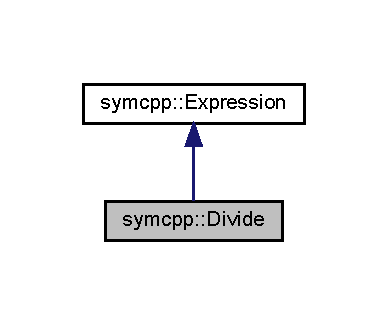
\includegraphics[width=186pt]{classsymcpp_1_1Divide__inherit__graph}
\end{center}
\end{figure}


Collaboration diagram for symcpp\+:\+:Divide\+:\nopagebreak
\begin{figure}[H]
\begin{center}
\leavevmode
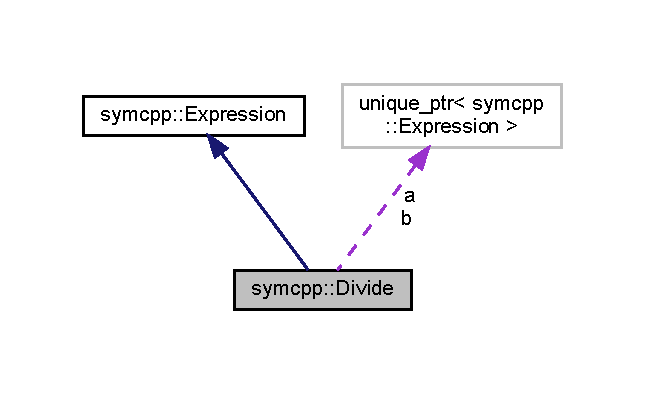
\includegraphics[width=310pt]{classsymcpp_1_1Divide__coll__graph}
\end{center}
\end{figure}
\subsection*{Public Member Functions}
\begin{DoxyCompactItemize}
\item 
\hyperlink{classsymcpp_1_1Divide_a1399cc15ca3af6ed217c20cadb2694ad}{Divide} (const \hyperlink{classsymcpp_1_1Expression}{Expression} \&\hyperlink{classsymcpp_1_1Divide_a52eaf8a705da4ef10b1fa2b87e76d0d8}{a}, const \hyperlink{classsymcpp_1_1Expression}{Expression} \&\hyperlink{classsymcpp_1_1Divide_a122c034c19635c036d39fbf18b1b8348}{b})
\item 
\hyperlink{classsymcpp_1_1Divide_a010b104132d0341805ca34277422d867}{Divide} (const std\+::unique\+\_\+ptr$<$ \hyperlink{classsymcpp_1_1Expression}{Expression} $>$ \&\hyperlink{classsymcpp_1_1Divide_a52eaf8a705da4ef10b1fa2b87e76d0d8}{a}, const std\+::unique\+\_\+ptr$<$ \hyperlink{classsymcpp_1_1Expression}{Expression} $>$ \&\hyperlink{classsymcpp_1_1Divide_a122c034c19635c036d39fbf18b1b8348}{b})
\item 
std\+::unique\+\_\+ptr$<$ \hyperlink{classsymcpp_1_1Expression}{Expression} $>$ \hyperlink{classsymcpp_1_1Divide_a6e4eeef806e8bded246e87d0036effee}{copy} () const override
\item 
std\+::unique\+\_\+ptr$<$ \hyperlink{classsymcpp_1_1Expression}{Expression} $>$ \hyperlink{classsymcpp_1_1Divide_aeecc60e1759b81ea65b0b95a62ff38df}{diff} (std\+::string v) const override
\item 
std\+::unique\+\_\+ptr$<$ \hyperlink{classsymcpp_1_1Expression}{Expression} $>$ \hyperlink{classsymcpp_1_1Divide_ab0e372a337f207a3e4c78fd1db9351a7}{simplify} () override
\item 
double \hyperlink{classsymcpp_1_1Divide_a85dcd571e1d2a188dcdc8090b7e90074}{subs} (const std\+::unordered\+\_\+map$<$ std\+::string, double $>$ \&env) const override
\item 
unsigned int \hyperlink{classsymcpp_1_1Divide_a016fec0e409cff8d0cd2b53eea1fa6c3}{precedence} () const override
\item 
bool \hyperlink{classsymcpp_1_1Divide_a342ddc6fb6f80a37797bda030b4c7580}{is\+\_\+constant} () const override
\item 
double \hyperlink{classsymcpp_1_1Divide_a18ab0e9eddd473ee5400607b9e6ea2b0}{const\+\_\+eval} () const override
\end{DoxyCompactItemize}
\subsection*{Private Member Functions}
\begin{DoxyCompactItemize}
\item 
std\+::ostream \& \hyperlink{classsymcpp_1_1Divide_a113a96148c27f2d50a596c782f9a4005}{print} (std\+::ostream \&sink) const override
\end{DoxyCompactItemize}
\subsection*{Private Attributes}
\begin{DoxyCompactItemize}
\item 
std\+::unique\+\_\+ptr$<$ \hyperlink{classsymcpp_1_1Expression}{Expression} $>$ \hyperlink{classsymcpp_1_1Divide_a52eaf8a705da4ef10b1fa2b87e76d0d8}{a}
\item 
std\+::unique\+\_\+ptr$<$ \hyperlink{classsymcpp_1_1Expression}{Expression} $>$ \hyperlink{classsymcpp_1_1Divide_a122c034c19635c036d39fbf18b1b8348}{b}
\end{DoxyCompactItemize}


\subsection{Constructor \& Destructor Documentation}
\index{symcpp\+::\+Divide@{symcpp\+::\+Divide}!Divide@{Divide}}
\index{Divide@{Divide}!symcpp\+::\+Divide@{symcpp\+::\+Divide}}
\subsubsection[{\texorpdfstring{Divide(const Expression \&a, const Expression \&b)}{Divide(const Expression &a, const Expression &b)}}]{\setlength{\rightskip}{0pt plus 5cm}symcpp\+::\+Divide\+::\+Divide (
\begin{DoxyParamCaption}
\item[{const {\bf Expression} \&}]{a, }
\item[{const {\bf Expression} \&}]{b}
\end{DoxyParamCaption}
)}\hypertarget{classsymcpp_1_1Divide_a1399cc15ca3af6ed217c20cadb2694ad}{}\label{classsymcpp_1_1Divide_a1399cc15ca3af6ed217c20cadb2694ad}
\index{symcpp\+::\+Divide@{symcpp\+::\+Divide}!Divide@{Divide}}
\index{Divide@{Divide}!symcpp\+::\+Divide@{symcpp\+::\+Divide}}
\subsubsection[{\texorpdfstring{Divide(const std\+::unique\+\_\+ptr$<$ Expression $>$ \&a, const std\+::unique\+\_\+ptr$<$ Expression $>$ \&b)}{Divide(const std::unique_ptr< Expression > &a, const std::unique_ptr< Expression > &b)}}]{\setlength{\rightskip}{0pt plus 5cm}symcpp\+::\+Divide\+::\+Divide (
\begin{DoxyParamCaption}
\item[{const std\+::unique\+\_\+ptr$<$ {\bf Expression} $>$ \&}]{a, }
\item[{const std\+::unique\+\_\+ptr$<$ {\bf Expression} $>$ \&}]{b}
\end{DoxyParamCaption}
)}\hypertarget{classsymcpp_1_1Divide_a010b104132d0341805ca34277422d867}{}\label{classsymcpp_1_1Divide_a010b104132d0341805ca34277422d867}


\subsection{Member Function Documentation}
\index{symcpp\+::\+Divide@{symcpp\+::\+Divide}!const\+\_\+eval@{const\+\_\+eval}}
\index{const\+\_\+eval@{const\+\_\+eval}!symcpp\+::\+Divide@{symcpp\+::\+Divide}}
\subsubsection[{\texorpdfstring{const\+\_\+eval() const override}{const_eval() const override}}]{\setlength{\rightskip}{0pt plus 5cm}double symcpp\+::\+Divide\+::const\+\_\+eval (
\begin{DoxyParamCaption}
{}
\end{DoxyParamCaption}
) const\hspace{0.3cm}{\ttfamily [override]}, {\ttfamily [virtual]}}\hypertarget{classsymcpp_1_1Divide_a18ab0e9eddd473ee5400607b9e6ea2b0}{}\label{classsymcpp_1_1Divide_a18ab0e9eddd473ee5400607b9e6ea2b0}


Implements \hyperlink{classsymcpp_1_1Expression_a81c8069347f586cb5632338d97c278ad}{symcpp\+::\+Expression}.

\index{symcpp\+::\+Divide@{symcpp\+::\+Divide}!copy@{copy}}
\index{copy@{copy}!symcpp\+::\+Divide@{symcpp\+::\+Divide}}
\subsubsection[{\texorpdfstring{copy() const override}{copy() const override}}]{\setlength{\rightskip}{0pt plus 5cm}std\+::unique\+\_\+ptr$<$ {\bf Expression} $>$ symcpp\+::\+Divide\+::copy (
\begin{DoxyParamCaption}
{}
\end{DoxyParamCaption}
) const\hspace{0.3cm}{\ttfamily [override]}, {\ttfamily [virtual]}}\hypertarget{classsymcpp_1_1Divide_a6e4eeef806e8bded246e87d0036effee}{}\label{classsymcpp_1_1Divide_a6e4eeef806e8bded246e87d0036effee}


Implements \hyperlink{classsymcpp_1_1Expression_a2e7de5a295ccf0efdc9b34cea7ba3d0b}{symcpp\+::\+Expression}.

\index{symcpp\+::\+Divide@{symcpp\+::\+Divide}!diff@{diff}}
\index{diff@{diff}!symcpp\+::\+Divide@{symcpp\+::\+Divide}}
\subsubsection[{\texorpdfstring{diff(std\+::string v) const override}{diff(std::string v) const override}}]{\setlength{\rightskip}{0pt plus 5cm}std\+::unique\+\_\+ptr$<$ {\bf Expression} $>$ symcpp\+::\+Divide\+::diff (
\begin{DoxyParamCaption}
\item[{std\+::string}]{v}
\end{DoxyParamCaption}
) const\hspace{0.3cm}{\ttfamily [override]}, {\ttfamily [virtual]}}\hypertarget{classsymcpp_1_1Divide_aeecc60e1759b81ea65b0b95a62ff38df}{}\label{classsymcpp_1_1Divide_aeecc60e1759b81ea65b0b95a62ff38df}


Implements \hyperlink{classsymcpp_1_1Expression_a032fe8da79d5e231ca2d21a201c8f32d}{symcpp\+::\+Expression}.

\index{symcpp\+::\+Divide@{symcpp\+::\+Divide}!is\+\_\+constant@{is\+\_\+constant}}
\index{is\+\_\+constant@{is\+\_\+constant}!symcpp\+::\+Divide@{symcpp\+::\+Divide}}
\subsubsection[{\texorpdfstring{is\+\_\+constant() const override}{is_constant() const override}}]{\setlength{\rightskip}{0pt plus 5cm}bool symcpp\+::\+Divide\+::is\+\_\+constant (
\begin{DoxyParamCaption}
{}
\end{DoxyParamCaption}
) const\hspace{0.3cm}{\ttfamily [override]}, {\ttfamily [virtual]}}\hypertarget{classsymcpp_1_1Divide_a342ddc6fb6f80a37797bda030b4c7580}{}\label{classsymcpp_1_1Divide_a342ddc6fb6f80a37797bda030b4c7580}


Implements \hyperlink{classsymcpp_1_1Expression_a30db7917c8948e22330cbe8259caeae2}{symcpp\+::\+Expression}.

\index{symcpp\+::\+Divide@{symcpp\+::\+Divide}!precedence@{precedence}}
\index{precedence@{precedence}!symcpp\+::\+Divide@{symcpp\+::\+Divide}}
\subsubsection[{\texorpdfstring{precedence() const override}{precedence() const override}}]{\setlength{\rightskip}{0pt plus 5cm}unsigned int symcpp\+::\+Divide\+::precedence (
\begin{DoxyParamCaption}
{}
\end{DoxyParamCaption}
) const\hspace{0.3cm}{\ttfamily [override]}, {\ttfamily [virtual]}}\hypertarget{classsymcpp_1_1Divide_a016fec0e409cff8d0cd2b53eea1fa6c3}{}\label{classsymcpp_1_1Divide_a016fec0e409cff8d0cd2b53eea1fa6c3}


Implements \hyperlink{classsymcpp_1_1Expression_a181c162d5740faac392ffdca26bfca0c}{symcpp\+::\+Expression}.

\index{symcpp\+::\+Divide@{symcpp\+::\+Divide}!print@{print}}
\index{print@{print}!symcpp\+::\+Divide@{symcpp\+::\+Divide}}
\subsubsection[{\texorpdfstring{print(std\+::ostream \&sink) const override}{print(std::ostream &sink) const override}}]{\setlength{\rightskip}{0pt plus 5cm}std\+::ostream \& symcpp\+::\+Divide\+::print (
\begin{DoxyParamCaption}
\item[{std\+::ostream \&}]{sink}
\end{DoxyParamCaption}
) const\hspace{0.3cm}{\ttfamily [override]}, {\ttfamily [private]}, {\ttfamily [virtual]}}\hypertarget{classsymcpp_1_1Divide_a113a96148c27f2d50a596c782f9a4005}{}\label{classsymcpp_1_1Divide_a113a96148c27f2d50a596c782f9a4005}


Implements \hyperlink{classsymcpp_1_1Expression_af37e13032a40f2da4d2866eaa8658049}{symcpp\+::\+Expression}.

\index{symcpp\+::\+Divide@{symcpp\+::\+Divide}!simplify@{simplify}}
\index{simplify@{simplify}!symcpp\+::\+Divide@{symcpp\+::\+Divide}}
\subsubsection[{\texorpdfstring{simplify() override}{simplify() override}}]{\setlength{\rightskip}{0pt plus 5cm}std\+::unique\+\_\+ptr$<$ {\bf Expression} $>$ symcpp\+::\+Divide\+::simplify (
\begin{DoxyParamCaption}
{}
\end{DoxyParamCaption}
)\hspace{0.3cm}{\ttfamily [override]}, {\ttfamily [virtual]}}\hypertarget{classsymcpp_1_1Divide_ab0e372a337f207a3e4c78fd1db9351a7}{}\label{classsymcpp_1_1Divide_ab0e372a337f207a3e4c78fd1db9351a7}


Implements \hyperlink{classsymcpp_1_1Expression_ab1fa6e55eea0682250d013f28db26cd2}{symcpp\+::\+Expression}.

\index{symcpp\+::\+Divide@{symcpp\+::\+Divide}!subs@{subs}}
\index{subs@{subs}!symcpp\+::\+Divide@{symcpp\+::\+Divide}}
\subsubsection[{\texorpdfstring{subs(const std\+::unordered\+\_\+map$<$ std\+::string, double $>$ \&env) const override}{subs(const std::unordered_map< std::string, double > &env) const override}}]{\setlength{\rightskip}{0pt plus 5cm}double symcpp\+::\+Divide\+::subs (
\begin{DoxyParamCaption}
\item[{const std\+::unordered\+\_\+map$<$ std\+::string, double $>$ \&}]{env}
\end{DoxyParamCaption}
) const\hspace{0.3cm}{\ttfamily [override]}, {\ttfamily [virtual]}}\hypertarget{classsymcpp_1_1Divide_a85dcd571e1d2a188dcdc8090b7e90074}{}\label{classsymcpp_1_1Divide_a85dcd571e1d2a188dcdc8090b7e90074}


Implements \hyperlink{classsymcpp_1_1Expression_aaef29b0afa2d6c21fe35f47a1be76134}{symcpp\+::\+Expression}.



\subsection{Member Data Documentation}
\index{symcpp\+::\+Divide@{symcpp\+::\+Divide}!a@{a}}
\index{a@{a}!symcpp\+::\+Divide@{symcpp\+::\+Divide}}
\subsubsection[{\texorpdfstring{a}{a}}]{\setlength{\rightskip}{0pt plus 5cm}std\+::unique\+\_\+ptr$<${\bf Expression}$>$ symcpp\+::\+Divide\+::a\hspace{0.3cm}{\ttfamily [private]}}\hypertarget{classsymcpp_1_1Divide_a52eaf8a705da4ef10b1fa2b87e76d0d8}{}\label{classsymcpp_1_1Divide_a52eaf8a705da4ef10b1fa2b87e76d0d8}
\index{symcpp\+::\+Divide@{symcpp\+::\+Divide}!b@{b}}
\index{b@{b}!symcpp\+::\+Divide@{symcpp\+::\+Divide}}
\subsubsection[{\texorpdfstring{b}{b}}]{\setlength{\rightskip}{0pt plus 5cm}std\+::unique\+\_\+ptr$<${\bf Expression}$>$ symcpp\+::\+Divide\+::b\hspace{0.3cm}{\ttfamily [private]}}\hypertarget{classsymcpp_1_1Divide_a122c034c19635c036d39fbf18b1b8348}{}\label{classsymcpp_1_1Divide_a122c034c19635c036d39fbf18b1b8348}


The documentation for this class was generated from the following files\+:\begin{DoxyCompactItemize}
\item 
src/symcpp/\hyperlink{Divide_8h}{Divide.\+h}\item 
src/symcpp/\hyperlink{Divide_8cpp}{Divide.\+cpp}\end{DoxyCompactItemize}

\hypertarget{classsymcpp_1_1Exponential}{}\section{symcpp\+::Exponential Class Reference}
\label{classsymcpp_1_1Exponential}\index{symcpp::Exponential@{symcpp::Exponential}}


{\ttfamily \#include $<$Exponential.\+h$>$}



Inheritance diagram for symcpp\+::Exponential\+:
\nopagebreak
\begin{figure}[H]
\begin{center}
\leavevmode
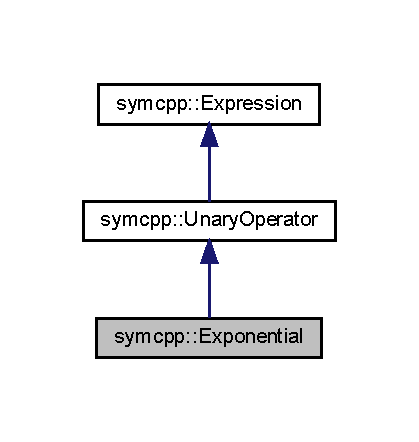
\includegraphics[width=201pt]{classsymcpp_1_1Exponential__inherit__graph}
\end{center}
\end{figure}


Collaboration diagram for symcpp\+::Exponential\+:
\nopagebreak
\begin{figure}[H]
\begin{center}
\leavevmode
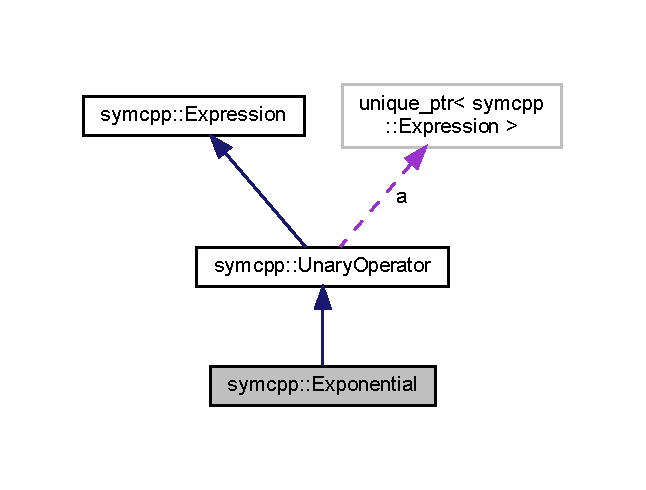
\includegraphics[width=310pt]{classsymcpp_1_1Exponential__coll__graph}
\end{center}
\end{figure}
\subsection*{Public Member Functions}
\begin{DoxyCompactItemize}
\item 
std\+::unique\+\_\+ptr$<$ \mbox{\hyperlink{classsymcpp_1_1Expression}{Expression}} $>$ \mbox{\hyperlink{classsymcpp_1_1Exponential_ad6ea3a357a471f75e28761c9a9f0d54d}{copy}} () const override
\item 
std\+::unique\+\_\+ptr$<$ \mbox{\hyperlink{classsymcpp_1_1Expression}{Expression}} $>$ \mbox{\hyperlink{classsymcpp_1_1Exponential_a099298ffa8721a8bb646d98518542d24}{simplify}} () override
\item 
\mbox{\hyperlink{classsymcpp_1_1Exponential_a23a8172db96675ebf1114f4f3f41b6f1}{Unary\+Operator}} (const \mbox{\hyperlink{classsymcpp_1_1Expression}{Expression}} \&\mbox{\hyperlink{classsymcpp_1_1UnaryOperator_a1558842963261562d2ef68e324822cba}{a}})
\item 
\mbox{\hyperlink{classsymcpp_1_1Exponential_ad3aa899567a080eeb41cb850de310178}{Unary\+Operator}} (std\+::unique\+\_\+ptr$<$ \mbox{\hyperlink{classsymcpp_1_1Expression}{Expression}} $>$ \&\&\mbox{\hyperlink{classsymcpp_1_1UnaryOperator_a1558842963261562d2ef68e324822cba}{a}})
\end{DoxyCompactItemize}
\subsection*{Private Member Functions}
\begin{DoxyCompactItemize}
\item 
double \mbox{\hyperlink{classsymcpp_1_1Exponential_aa36daedb8bf7bfe74f7f5ef85e448a7f}{op}} (double x) const override
\item 
std\+::ostream \& \mbox{\hyperlink{classsymcpp_1_1Exponential_a2af4d6f507139799516d960293f74343}{print}} (std\+::ostream \&sink) const override
\item 
std\+::unique\+\_\+ptr$<$ \mbox{\hyperlink{classsymcpp_1_1Expression}{Expression}} $>$ \mbox{\hyperlink{classsymcpp_1_1Exponential_a73f9208294626b48e2385a08e761b846}{partial\+\_\+derivative}} () const override
\end{DoxyCompactItemize}
\subsection*{Additional Inherited Members}


\subsection{Member Function Documentation}
\mbox{\Hypertarget{classsymcpp_1_1Exponential_ad6ea3a357a471f75e28761c9a9f0d54d}\label{classsymcpp_1_1Exponential_ad6ea3a357a471f75e28761c9a9f0d54d}} 
\index{symcpp::Exponential@{symcpp::Exponential}!copy@{copy}}
\index{copy@{copy}!symcpp::Exponential@{symcpp::Exponential}}
\subsubsection{\texorpdfstring{copy()}{copy()}}
{\footnotesize\ttfamily std\+::unique\+\_\+ptr$<$ \mbox{\hyperlink{classsymcpp_1_1Expression}{Expression}} $>$ symcpp\+::\+Exponential\+::copy (\begin{DoxyParamCaption}{ }\end{DoxyParamCaption}) const\hspace{0.3cm}{\ttfamily [override]}, {\ttfamily [virtual]}}



Implements \mbox{\hyperlink{classsymcpp_1_1Expression_a2e7de5a295ccf0efdc9b34cea7ba3d0b}{symcpp\+::\+Expression}}.

\mbox{\Hypertarget{classsymcpp_1_1Exponential_aa36daedb8bf7bfe74f7f5ef85e448a7f}\label{classsymcpp_1_1Exponential_aa36daedb8bf7bfe74f7f5ef85e448a7f}} 
\index{symcpp::Exponential@{symcpp::Exponential}!op@{op}}
\index{op@{op}!symcpp::Exponential@{symcpp::Exponential}}
\subsubsection{\texorpdfstring{op()}{op()}}
{\footnotesize\ttfamily double symcpp\+::\+Exponential\+::op (\begin{DoxyParamCaption}\item[{double}]{x }\end{DoxyParamCaption}) const\hspace{0.3cm}{\ttfamily [override]}, {\ttfamily [private]}, {\ttfamily [virtual]}}



Implements \mbox{\hyperlink{classsymcpp_1_1UnaryOperator_a679c3c46cad3a62bdd776ff836c7891e}{symcpp\+::\+Unary\+Operator}}.

\mbox{\Hypertarget{classsymcpp_1_1Exponential_a73f9208294626b48e2385a08e761b846}\label{classsymcpp_1_1Exponential_a73f9208294626b48e2385a08e761b846}} 
\index{symcpp::Exponential@{symcpp::Exponential}!partial\_derivative@{partial\_derivative}}
\index{partial\_derivative@{partial\_derivative}!symcpp::Exponential@{symcpp::Exponential}}
\subsubsection{\texorpdfstring{partial\_derivative()}{partial\_derivative()}}
{\footnotesize\ttfamily std\+::unique\+\_\+ptr$<$ \mbox{\hyperlink{classsymcpp_1_1Expression}{Expression}} $>$ symcpp\+::\+Exponential\+::partial\+\_\+derivative (\begin{DoxyParamCaption}{ }\end{DoxyParamCaption}) const\hspace{0.3cm}{\ttfamily [override]}, {\ttfamily [private]}, {\ttfamily [virtual]}}



Implements \mbox{\hyperlink{classsymcpp_1_1UnaryOperator_a85de3214870cd72edc63ac1c221ddeee}{symcpp\+::\+Unary\+Operator}}.

\mbox{\Hypertarget{classsymcpp_1_1Exponential_a2af4d6f507139799516d960293f74343}\label{classsymcpp_1_1Exponential_a2af4d6f507139799516d960293f74343}} 
\index{symcpp::Exponential@{symcpp::Exponential}!print@{print}}
\index{print@{print}!symcpp::Exponential@{symcpp::Exponential}}
\subsubsection{\texorpdfstring{print()}{print()}}
{\footnotesize\ttfamily std\+::ostream \& symcpp\+::\+Exponential\+::print (\begin{DoxyParamCaption}\item[{std\+::ostream \&}]{sink }\end{DoxyParamCaption}) const\hspace{0.3cm}{\ttfamily [override]}, {\ttfamily [private]}, {\ttfamily [virtual]}}



Implements \mbox{\hyperlink{classsymcpp_1_1Expression_af37e13032a40f2da4d2866eaa8658049}{symcpp\+::\+Expression}}.

\mbox{\Hypertarget{classsymcpp_1_1Exponential_a099298ffa8721a8bb646d98518542d24}\label{classsymcpp_1_1Exponential_a099298ffa8721a8bb646d98518542d24}} 
\index{symcpp::Exponential@{symcpp::Exponential}!simplify@{simplify}}
\index{simplify@{simplify}!symcpp::Exponential@{symcpp::Exponential}}
\subsubsection{\texorpdfstring{simplify()}{simplify()}}
{\footnotesize\ttfamily std\+::unique\+\_\+ptr$<$ \mbox{\hyperlink{classsymcpp_1_1Expression}{Expression}} $>$ symcpp\+::\+Exponential\+::simplify (\begin{DoxyParamCaption}{ }\end{DoxyParamCaption})\hspace{0.3cm}{\ttfamily [override]}, {\ttfamily [virtual]}}



Implements \mbox{\hyperlink{classsymcpp_1_1Expression_ab1fa6e55eea0682250d013f28db26cd2}{symcpp\+::\+Expression}}.

\mbox{\Hypertarget{classsymcpp_1_1Exponential_ad3aa899567a080eeb41cb850de310178}\label{classsymcpp_1_1Exponential_ad3aa899567a080eeb41cb850de310178}} 
\index{symcpp::Exponential@{symcpp::Exponential}!UnaryOperator@{UnaryOperator}}
\index{UnaryOperator@{UnaryOperator}!symcpp::Exponential@{symcpp::Exponential}}
\subsubsection{\texorpdfstring{UnaryOperator()}{UnaryOperator()}\hspace{0.1cm}{\footnotesize\ttfamily [1/2]}}
{\footnotesize\ttfamily symcpp\+::\+Unary\+Operator\+::\+Unary\+Operator\hspace{0.3cm}{\ttfamily [inline]}}

\mbox{\Hypertarget{classsymcpp_1_1Exponential_a23a8172db96675ebf1114f4f3f41b6f1}\label{classsymcpp_1_1Exponential_a23a8172db96675ebf1114f4f3f41b6f1}} 
\index{symcpp::Exponential@{symcpp::Exponential}!UnaryOperator@{UnaryOperator}}
\index{UnaryOperator@{UnaryOperator}!symcpp::Exponential@{symcpp::Exponential}}
\subsubsection{\texorpdfstring{UnaryOperator()}{UnaryOperator()}\hspace{0.1cm}{\footnotesize\ttfamily [2/2]}}
{\footnotesize\ttfamily symcpp\+::\+Unary\+Operator\+::\+Unary\+Operator\hspace{0.3cm}{\ttfamily [inline]}}



The documentation for this class was generated from the following files\+:\begin{DoxyCompactItemize}
\item 
src/symcpp/\mbox{\hyperlink{Exponential_8h}{Exponential.\+h}}\item 
src/symcpp/\mbox{\hyperlink{Exponential_8cpp}{Exponential.\+cpp}}\end{DoxyCompactItemize}

\hypertarget{classsymcpp_1_1Expression}{}\section{symcpp\+:\+:Expression Class Reference}
\label{classsymcpp_1_1Expression}\index{symcpp\+::\+Expression@{symcpp\+::\+Expression}}


{\ttfamily \#include $<$Expression.\+h$>$}



Inheritance diagram for symcpp\+:\+:Expression\+:\nopagebreak
\begin{figure}[H]
\begin{center}
\leavevmode
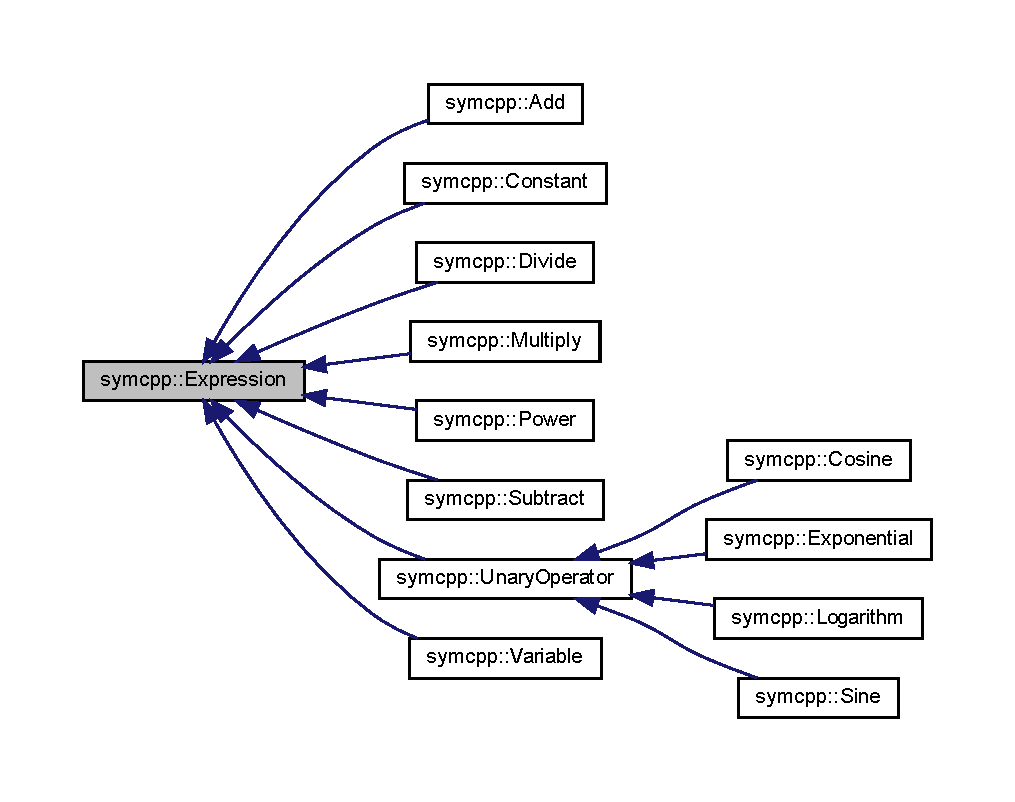
\includegraphics[width=350pt]{classsymcpp_1_1Expression__inherit__graph}
\end{center}
\end{figure}
\subsection*{Public Member Functions}
\begin{DoxyCompactItemize}
\item 
virtual double \hyperlink{classsymcpp_1_1Expression_aaef29b0afa2d6c21fe35f47a1be76134}{subs} (const std\+::unordered\+\_\+map$<$ std\+::string, double $>$ \&env) const =0
\item 
virtual std\+::unique\+\_\+ptr$<$ \hyperlink{classsymcpp_1_1Expression}{Expression} $>$ \hyperlink{classsymcpp_1_1Expression_a032fe8da79d5e231ca2d21a201c8f32d}{diff} (std\+::string var) const =0
\item 
virtual std\+::unique\+\_\+ptr$<$ \hyperlink{classsymcpp_1_1Expression}{Expression} $>$ \hyperlink{classsymcpp_1_1Expression_a2e7de5a295ccf0efdc9b34cea7ba3d0b}{copy} () const =0
\item 
virtual std\+::unique\+\_\+ptr$<$ \hyperlink{classsymcpp_1_1Expression}{Expression} $>$ \hyperlink{classsymcpp_1_1Expression_ab1fa6e55eea0682250d013f28db26cd2}{simplify} ()=0
\item 
virtual bool \hyperlink{classsymcpp_1_1Expression_a30db7917c8948e22330cbe8259caeae2}{is\+\_\+constant} () const =0
\item 
virtual unsigned int \hyperlink{classsymcpp_1_1Expression_a181c162d5740faac392ffdca26bfca0c}{precedence} () const =0
\item 
virtual double \hyperlink{classsymcpp_1_1Expression_a81c8069347f586cb5632338d97c278ad}{const\+\_\+eval} () const =0
\end{DoxyCompactItemize}
\subsection*{Private Member Functions}
\begin{DoxyCompactItemize}
\item 
virtual std\+::ostream \& \hyperlink{classsymcpp_1_1Expression_af37e13032a40f2da4d2866eaa8658049}{print} (std\+::ostream \&sink) const =0
\end{DoxyCompactItemize}
\subsection*{Friends}
\begin{DoxyCompactItemize}
\item 
std\+::ostream \& \hyperlink{classsymcpp_1_1Expression_ade0d81d94acc2274ae8657f14d5636fe}{operator$<$$<$} (std\+::ostream \&sink, const \hyperlink{classsymcpp_1_1Expression}{Expression} \&expr)
\end{DoxyCompactItemize}


\subsection{Member Function Documentation}
\index{symcpp\+::\+Expression@{symcpp\+::\+Expression}!const\+\_\+eval@{const\+\_\+eval}}
\index{const\+\_\+eval@{const\+\_\+eval}!symcpp\+::\+Expression@{symcpp\+::\+Expression}}
\subsubsection[{\texorpdfstring{const\+\_\+eval() const =0}{const_eval() const =0}}]{\setlength{\rightskip}{0pt plus 5cm}virtual double symcpp\+::\+Expression\+::const\+\_\+eval (
\begin{DoxyParamCaption}
{}
\end{DoxyParamCaption}
) const\hspace{0.3cm}{\ttfamily [pure virtual]}}\hypertarget{classsymcpp_1_1Expression_a81c8069347f586cb5632338d97c278ad}{}\label{classsymcpp_1_1Expression_a81c8069347f586cb5632338d97c278ad}


Implemented in \hyperlink{classsymcpp_1_1Power_ac344573e85b3db4a324ba3635244c8ca}{symcpp\+::\+Power}, \hyperlink{classsymcpp_1_1Add_af3e5c83af088ffc00849e852e18b055c}{symcpp\+::\+Add}, \hyperlink{classsymcpp_1_1Divide_a18ab0e9eddd473ee5400607b9e6ea2b0}{symcpp\+::\+Divide}, \hyperlink{classsymcpp_1_1Multiply_a1d9b8023ab0bf35c011eb7f3ee8d4c32}{symcpp\+::\+Multiply}, \hyperlink{classsymcpp_1_1Constant_a9c2a9089ae171c2403e053a566929b45}{symcpp\+::\+Constant}, \hyperlink{classsymcpp_1_1Subtract_a619e8733e2b9c07f9bcdb1c82781fad9}{symcpp\+::\+Subtract}, \hyperlink{classsymcpp_1_1Variable_a822c9e3e85da6e89949a9f2df7244f5c}{symcpp\+::\+Variable}, and \hyperlink{classsymcpp_1_1UnaryOperator_ae44aa26276abde61e16be12814075d0a}{symcpp\+::\+Unary\+Operator}.

\index{symcpp\+::\+Expression@{symcpp\+::\+Expression}!copy@{copy}}
\index{copy@{copy}!symcpp\+::\+Expression@{symcpp\+::\+Expression}}
\subsubsection[{\texorpdfstring{copy() const =0}{copy() const =0}}]{\setlength{\rightskip}{0pt plus 5cm}virtual std\+::unique\+\_\+ptr$<${\bf Expression}$>$ symcpp\+::\+Expression\+::copy (
\begin{DoxyParamCaption}
{}
\end{DoxyParamCaption}
) const\hspace{0.3cm}{\ttfamily [pure virtual]}}\hypertarget{classsymcpp_1_1Expression_a2e7de5a295ccf0efdc9b34cea7ba3d0b}{}\label{classsymcpp_1_1Expression_a2e7de5a295ccf0efdc9b34cea7ba3d0b}


Implemented in \hyperlink{classsymcpp_1_1Power_ac628b9070382bde67b838f291f81ddc4}{symcpp\+::\+Power}, \hyperlink{classsymcpp_1_1Add_a58633f0c101ef1e7cc3952846054d27f}{symcpp\+::\+Add}, \hyperlink{classsymcpp_1_1Subtract_a97b707b4c72caa44342fe7952d616a4d}{symcpp\+::\+Subtract}, \hyperlink{classsymcpp_1_1Cosine_a63c4510666729dfcf5727299945c60f5}{symcpp\+::\+Cosine}, \hyperlink{classsymcpp_1_1Divide_a6e4eeef806e8bded246e87d0036effee}{symcpp\+::\+Divide}, \hyperlink{classsymcpp_1_1Multiply_adcd57ab1c1a27eb10aeeb572cdd14e5e}{symcpp\+::\+Multiply}, \hyperlink{classsymcpp_1_1Sine_aab90ccee3ae1fd2d832bdf041e8352c6}{symcpp\+::\+Sine}, \hyperlink{classsymcpp_1_1Exponential_ad6ea3a357a471f75e28761c9a9f0d54d}{symcpp\+::\+Exponential}, \hyperlink{classsymcpp_1_1Constant_aa5a5b0f6f06e6017ed641e8b89cd0cef}{symcpp\+::\+Constant}, \hyperlink{classsymcpp_1_1Logarithm_ac7315464088f7ef34cfce74e518b939a}{symcpp\+::\+Logarithm}, and \hyperlink{classsymcpp_1_1Variable_a5a434805a53a7c46e3659a8efdc7ba80}{symcpp\+::\+Variable}.

\index{symcpp\+::\+Expression@{symcpp\+::\+Expression}!diff@{diff}}
\index{diff@{diff}!symcpp\+::\+Expression@{symcpp\+::\+Expression}}
\subsubsection[{\texorpdfstring{diff(std\+::string var) const =0}{diff(std::string var) const =0}}]{\setlength{\rightskip}{0pt plus 5cm}virtual std\+::unique\+\_\+ptr$<${\bf Expression}$>$ symcpp\+::\+Expression\+::diff (
\begin{DoxyParamCaption}
\item[{std\+::string}]{var}
\end{DoxyParamCaption}
) const\hspace{0.3cm}{\ttfamily [pure virtual]}}\hypertarget{classsymcpp_1_1Expression_a032fe8da79d5e231ca2d21a201c8f32d}{}\label{classsymcpp_1_1Expression_a032fe8da79d5e231ca2d21a201c8f32d}


Implemented in \hyperlink{classsymcpp_1_1Power_ac8fdf5b0ddfa04647ba93a6c383d4a7b}{symcpp\+::\+Power}, \hyperlink{classsymcpp_1_1Add_ac885da5635431d264c643618729f6cec}{symcpp\+::\+Add}, \hyperlink{classsymcpp_1_1Divide_aeecc60e1759b81ea65b0b95a62ff38df}{symcpp\+::\+Divide}, \hyperlink{classsymcpp_1_1Multiply_a835e55ada54a6c1eeb6d02ceeef83198}{symcpp\+::\+Multiply}, \hyperlink{classsymcpp_1_1Subtract_a4f9040e23694efcf093bf4b5c59b386b}{symcpp\+::\+Subtract}, \hyperlink{classsymcpp_1_1Constant_a19dd15712ce8630b758766e6478dec58}{symcpp\+::\+Constant}, \hyperlink{classsymcpp_1_1UnaryOperator_a73f6af837c67e65504e4bb82111d9557}{symcpp\+::\+Unary\+Operator}, and \hyperlink{classsymcpp_1_1Variable_ae17a02824954066f4e8b1ed6ba799ff0}{symcpp\+::\+Variable}.

\index{symcpp\+::\+Expression@{symcpp\+::\+Expression}!is\+\_\+constant@{is\+\_\+constant}}
\index{is\+\_\+constant@{is\+\_\+constant}!symcpp\+::\+Expression@{symcpp\+::\+Expression}}
\subsubsection[{\texorpdfstring{is\+\_\+constant() const =0}{is_constant() const =0}}]{\setlength{\rightskip}{0pt plus 5cm}virtual bool symcpp\+::\+Expression\+::is\+\_\+constant (
\begin{DoxyParamCaption}
{}
\end{DoxyParamCaption}
) const\hspace{0.3cm}{\ttfamily [pure virtual]}}\hypertarget{classsymcpp_1_1Expression_a30db7917c8948e22330cbe8259caeae2}{}\label{classsymcpp_1_1Expression_a30db7917c8948e22330cbe8259caeae2}


Implemented in \hyperlink{classsymcpp_1_1Subtract_a651ca7fc5e804970141b65813e738463}{symcpp\+::\+Subtract}, \hyperlink{classsymcpp_1_1Add_a6a9286402a1b24bf3a7c1ed348357875}{symcpp\+::\+Add}, \hyperlink{classsymcpp_1_1Divide_a342ddc6fb6f80a37797bda030b4c7580}{symcpp\+::\+Divide}, \hyperlink{classsymcpp_1_1Power_af90cd850099fda788416ab5aa9e752e2}{symcpp\+::\+Power}, \hyperlink{classsymcpp_1_1Constant_af1ae4532a85ec5c5ed55ed8d69be68b3}{symcpp\+::\+Constant}, \hyperlink{classsymcpp_1_1Multiply_a771fc25f8bafd49600c31db11dd72256}{symcpp\+::\+Multiply}, \hyperlink{classsymcpp_1_1Variable_a1ccd5094922661828039f16b77974fe0}{symcpp\+::\+Variable}, and \hyperlink{classsymcpp_1_1UnaryOperator_abb499ba635a63dfa605fc3639509ac1c}{symcpp\+::\+Unary\+Operator}.

\index{symcpp\+::\+Expression@{symcpp\+::\+Expression}!precedence@{precedence}}
\index{precedence@{precedence}!symcpp\+::\+Expression@{symcpp\+::\+Expression}}
\subsubsection[{\texorpdfstring{precedence() const =0}{precedence() const =0}}]{\setlength{\rightskip}{0pt plus 5cm}virtual unsigned int symcpp\+::\+Expression\+::precedence (
\begin{DoxyParamCaption}
{}
\end{DoxyParamCaption}
) const\hspace{0.3cm}{\ttfamily [pure virtual]}}\hypertarget{classsymcpp_1_1Expression_a181c162d5740faac392ffdca26bfca0c}{}\label{classsymcpp_1_1Expression_a181c162d5740faac392ffdca26bfca0c}


Implemented in \hyperlink{classsymcpp_1_1Power_a1287f36d506b82695187beae3f3c9a5e}{symcpp\+::\+Power}, \hyperlink{classsymcpp_1_1Add_aec3ebe2c1bde461d8bd086e9c87aeeed}{symcpp\+::\+Add}, \hyperlink{classsymcpp_1_1Divide_a016fec0e409cff8d0cd2b53eea1fa6c3}{symcpp\+::\+Divide}, \hyperlink{classsymcpp_1_1Subtract_ac0b20c29aac75772aeb226eec86ffc22}{symcpp\+::\+Subtract}, \hyperlink{classsymcpp_1_1Constant_a8c5e1e1b0cb2131d6f20b118f32a223f}{symcpp\+::\+Constant}, \hyperlink{classsymcpp_1_1Multiply_afd9f779b82aa2d7a3be63e7b8b0e8eb1}{symcpp\+::\+Multiply}, \hyperlink{classsymcpp_1_1Variable_a4b998019a17f29482772f1f945398ff3}{symcpp\+::\+Variable}, and \hyperlink{classsymcpp_1_1UnaryOperator_a129a9c47390abceff31da35d7b847329}{symcpp\+::\+Unary\+Operator}.

\index{symcpp\+::\+Expression@{symcpp\+::\+Expression}!print@{print}}
\index{print@{print}!symcpp\+::\+Expression@{symcpp\+::\+Expression}}
\subsubsection[{\texorpdfstring{print(std\+::ostream \&sink) const =0}{print(std::ostream &sink) const =0}}]{\setlength{\rightskip}{0pt plus 5cm}virtual std\+::ostream\& symcpp\+::\+Expression\+::print (
\begin{DoxyParamCaption}
\item[{std\+::ostream \&}]{sink}
\end{DoxyParamCaption}
) const\hspace{0.3cm}{\ttfamily [private]}, {\ttfamily [pure virtual]}}\hypertarget{classsymcpp_1_1Expression_af37e13032a40f2da4d2866eaa8658049}{}\label{classsymcpp_1_1Expression_af37e13032a40f2da4d2866eaa8658049}


Implemented in \hyperlink{classsymcpp_1_1Power_aeddeec10b104818656e7f2f1536abccc}{symcpp\+::\+Power}, \hyperlink{classsymcpp_1_1Add_a4e73df4d72972d00ab139c5db4a93a0b}{symcpp\+::\+Add}, \hyperlink{classsymcpp_1_1Divide_a113a96148c27f2d50a596c782f9a4005}{symcpp\+::\+Divide}, \hyperlink{classsymcpp_1_1Multiply_a8d6dbfc85d0609f40d52c0fc853a06b5}{symcpp\+::\+Multiply}, \hyperlink{classsymcpp_1_1Subtract_a7f0af9519d3a4978abf85e88da7d682d}{symcpp\+::\+Subtract}, \hyperlink{classsymcpp_1_1Constant_aca89e2af8df740dba562776e389edab6}{symcpp\+::\+Constant}, \hyperlink{classsymcpp_1_1Variable_a10ce030c1648fae51534712155ffcab1}{symcpp\+::\+Variable}, \hyperlink{classsymcpp_1_1Exponential_a2af4d6f507139799516d960293f74343}{symcpp\+::\+Exponential}, \hyperlink{classsymcpp_1_1Logarithm_a336bed1a474b338eabd6a258d527b65b}{symcpp\+::\+Logarithm}, \hyperlink{classsymcpp_1_1Cosine_a2d8d4dc8d5119d59365f212b7d855a53}{symcpp\+::\+Cosine}, and \hyperlink{classsymcpp_1_1Sine_ad3680056460c4990115a23427ea723fe}{symcpp\+::\+Sine}.

\index{symcpp\+::\+Expression@{symcpp\+::\+Expression}!simplify@{simplify}}
\index{simplify@{simplify}!symcpp\+::\+Expression@{symcpp\+::\+Expression}}
\subsubsection[{\texorpdfstring{simplify()=0}{simplify()=0}}]{\setlength{\rightskip}{0pt plus 5cm}virtual std\+::unique\+\_\+ptr$<${\bf Expression}$>$ symcpp\+::\+Expression\+::simplify (
\begin{DoxyParamCaption}
{}
\end{DoxyParamCaption}
)\hspace{0.3cm}{\ttfamily [pure virtual]}}\hypertarget{classsymcpp_1_1Expression_ab1fa6e55eea0682250d013f28db26cd2}{}\label{classsymcpp_1_1Expression_ab1fa6e55eea0682250d013f28db26cd2}


Implemented in \hyperlink{classsymcpp_1_1Multiply_aff728e2edaa447f154918079b4e35a7e}{symcpp\+::\+Multiply}, \hyperlink{classsymcpp_1_1Power_aa6411b410decc9778640feaa7d173349}{symcpp\+::\+Power}, \hyperlink{classsymcpp_1_1Add_a5a68fdd76c2206399dd5a78c4b317505}{symcpp\+::\+Add}, \hyperlink{classsymcpp_1_1Subtract_a3d3b5586c41dbbee1071a08db5725ecc}{symcpp\+::\+Subtract}, \hyperlink{classsymcpp_1_1Divide_ab0e372a337f207a3e4c78fd1db9351a7}{symcpp\+::\+Divide}, \hyperlink{classsymcpp_1_1Constant_a082044c6d521c2d31bbadd5db6354f96}{symcpp\+::\+Constant}, \hyperlink{classsymcpp_1_1Variable_afd613d28c73d738fc0cf90b70e1820bb}{symcpp\+::\+Variable}, \hyperlink{classsymcpp_1_1Exponential_a099298ffa8721a8bb646d98518542d24}{symcpp\+::\+Exponential}, \hyperlink{classsymcpp_1_1Logarithm_af771894e90cbe561e3eb2e9a9b32954b}{symcpp\+::\+Logarithm}, \hyperlink{classsymcpp_1_1Cosine_a8bedd5e4ad3245d5ee6e6e7da3b5e8dc}{symcpp\+::\+Cosine}, and \hyperlink{classsymcpp_1_1Sine_a3cac7091905da6765a019a0ece9e45d5}{symcpp\+::\+Sine}.

\index{symcpp\+::\+Expression@{symcpp\+::\+Expression}!subs@{subs}}
\index{subs@{subs}!symcpp\+::\+Expression@{symcpp\+::\+Expression}}
\subsubsection[{\texorpdfstring{subs(const std\+::unordered\+\_\+map$<$ std\+::string, double $>$ \&env) const =0}{subs(const std::unordered_map< std::string, double > &env) const =0}}]{\setlength{\rightskip}{0pt plus 5cm}virtual double symcpp\+::\+Expression\+::subs (
\begin{DoxyParamCaption}
\item[{const std\+::unordered\+\_\+map$<$ std\+::string, double $>$ \&}]{env}
\end{DoxyParamCaption}
) const\hspace{0.3cm}{\ttfamily [pure virtual]}}\hypertarget{classsymcpp_1_1Expression_aaef29b0afa2d6c21fe35f47a1be76134}{}\label{classsymcpp_1_1Expression_aaef29b0afa2d6c21fe35f47a1be76134}


Implemented in \hyperlink{classsymcpp_1_1Divide_a85dcd571e1d2a188dcdc8090b7e90074}{symcpp\+::\+Divide}, \hyperlink{classsymcpp_1_1Constant_ac6f62c3945429d0d318dc7d366dd4b54}{symcpp\+::\+Constant}, \hyperlink{classsymcpp_1_1Multiply_a83a9396b931cd5010630f48ecd1bc2a1}{symcpp\+::\+Multiply}, \hyperlink{classsymcpp_1_1Variable_a1dfbef67a237aa2533d8dc88c378d08b}{symcpp\+::\+Variable}, \hyperlink{classsymcpp_1_1Power_a0cf64595eca511f6a83317f47754bd58}{symcpp\+::\+Power}, \hyperlink{classsymcpp_1_1UnaryOperator_aa2296c73f9ca24a739fb8c3ff246fe0e}{symcpp\+::\+Unary\+Operator}, \hyperlink{classsymcpp_1_1Add_a79d0aa670728ba4a257e777ed4ac1ec0}{symcpp\+::\+Add}, and \hyperlink{classsymcpp_1_1Subtract_a35a24632dfacadb23e4177a539e7c1df}{symcpp\+::\+Subtract}.



\subsection{Friends And Related Function Documentation}
\index{symcpp\+::\+Expression@{symcpp\+::\+Expression}!operator$<$$<$@{operator$<$$<$}}
\index{operator$<$$<$@{operator$<$$<$}!symcpp\+::\+Expression@{symcpp\+::\+Expression}}
\subsubsection[{\texorpdfstring{operator$<$$<$}{operator<<}}]{\setlength{\rightskip}{0pt plus 5cm}std\+::ostream\& operator$<$$<$ (
\begin{DoxyParamCaption}
\item[{std\+::ostream \&}]{sink, }
\item[{const {\bf Expression} \&}]{expr}
\end{DoxyParamCaption}
)\hspace{0.3cm}{\ttfamily [friend]}}\hypertarget{classsymcpp_1_1Expression_ade0d81d94acc2274ae8657f14d5636fe}{}\label{classsymcpp_1_1Expression_ade0d81d94acc2274ae8657f14d5636fe}


The documentation for this class was generated from the following file\+:\begin{DoxyCompactItemize}
\item 
src/symcpp/\hyperlink{Expression_8h}{Expression.\+h}\end{DoxyCompactItemize}

\hypertarget{structFaceData}{}\section{Face\+Data Struct Reference}
\label{structFaceData}\index{FaceData@{FaceData}}


{\ttfamily \#include $<$O\+B\+J\+File.\+h$>$}



Collaboration diagram for Face\+Data\+:
\nopagebreak
\begin{figure}[H]
\begin{center}
\leavevmode
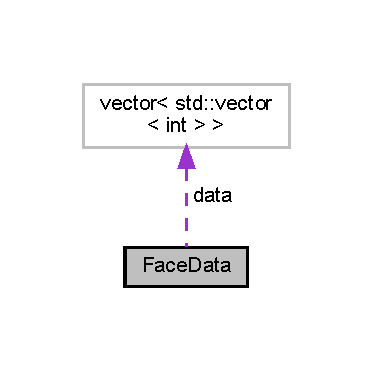
\includegraphics[width=179pt]{structFaceData__coll__graph}
\end{center}
\end{figure}
\subsection*{Public Member Functions}
\begin{DoxyCompactItemize}
\item 
\mbox{\hyperlink{structFaceData_a551092a23b9870e60bb840e6079f786d}{Face\+Data}} (std\+::istringstream \&iss)
\item 
std\+::vector$<$ \mbox{\hyperlink{classTriangle}{Triangle}} $>$ \mbox{\hyperlink{structFaceData_a641796d91855ab809b4b56e563b53be2}{get\+\_\+triangles}} (const std\+::vector$<$ \mbox{\hyperlink{classVector3D}{Vector3D}} $>$ \&vertices, const std\+::vector$<$ \mbox{\hyperlink{classVector3D}{Vector3D}} $>$ \&normals, \mbox{\hyperlink{classMaterial}{Material}} mat)
\end{DoxyCompactItemize}
\subsection*{Public Attributes}
\begin{DoxyCompactItemize}
\item 
std\+::vector$<$ std\+::vector$<$ int $>$ $>$ \mbox{\hyperlink{structFaceData_adb2e792d840b92f060ea4c615a91b0c3}{data}}
\end{DoxyCompactItemize}


\subsection{Constructor \& Destructor Documentation}
\mbox{\Hypertarget{structFaceData_a551092a23b9870e60bb840e6079f786d}\label{structFaceData_a551092a23b9870e60bb840e6079f786d}} 
\index{FaceData@{FaceData}!FaceData@{FaceData}}
\index{FaceData@{FaceData}!FaceData@{FaceData}}
\subsubsection{\texorpdfstring{FaceData()}{FaceData()}}
{\footnotesize\ttfamily Face\+Data\+::\+Face\+Data (\begin{DoxyParamCaption}\item[{std\+::istringstream \&}]{iss }\end{DoxyParamCaption})}



\subsection{Member Function Documentation}
\mbox{\Hypertarget{structFaceData_a641796d91855ab809b4b56e563b53be2}\label{structFaceData_a641796d91855ab809b4b56e563b53be2}} 
\index{FaceData@{FaceData}!get\_triangles@{get\_triangles}}
\index{get\_triangles@{get\_triangles}!FaceData@{FaceData}}
\subsubsection{\texorpdfstring{get\_triangles()}{get\_triangles()}}
{\footnotesize\ttfamily std\+::vector$<$ \mbox{\hyperlink{classTriangle}{Triangle}} $>$ Face\+Data\+::get\+\_\+triangles (\begin{DoxyParamCaption}\item[{const std\+::vector$<$ \mbox{\hyperlink{classVector3D}{Vector3D}} $>$ \&}]{vertices,  }\item[{const std\+::vector$<$ \mbox{\hyperlink{classVector3D}{Vector3D}} $>$ \&}]{normals,  }\item[{\mbox{\hyperlink{classMaterial}{Material}}}]{mat }\end{DoxyParamCaption})}



\subsection{Member Data Documentation}
\mbox{\Hypertarget{structFaceData_adb2e792d840b92f060ea4c615a91b0c3}\label{structFaceData_adb2e792d840b92f060ea4c615a91b0c3}} 
\index{FaceData@{FaceData}!data@{data}}
\index{data@{data}!FaceData@{FaceData}}
\subsubsection{\texorpdfstring{data}{data}}
{\footnotesize\ttfamily std\+::vector$<$std\+::vector$<$int$>$ $>$ Face\+Data\+::data}



The documentation for this struct was generated from the following files\+:\begin{DoxyCompactItemize}
\item 
src/\mbox{\hyperlink{OBJFile_8h}{O\+B\+J\+File.\+h}}\item 
src/\mbox{\hyperlink{OBJFile_8cpp}{O\+B\+J\+File.\+cpp}}\end{DoxyCompactItemize}

\hypertarget{classFixedSizeStack}{}\section{Fixed\+Size\+Stack$<$ V, N $>$ Class Template Reference}
\label{classFixedSizeStack}\index{Fixed\+Size\+Stack$<$ V, N $>$@{Fixed\+Size\+Stack$<$ V, N $>$}}


A stack that can contain at most N elements. If more are pushed to the stack, it will crash. No error handling is done. If top is called on an empty stack, it will crash.  




{\ttfamily \#include $<$Binary\+Volume\+Hierarchy.\+h$>$}



Collaboration diagram for Fixed\+Size\+Stack$<$ V, N $>$\+:\nopagebreak
\begin{figure}[H]
\begin{center}
\leavevmode
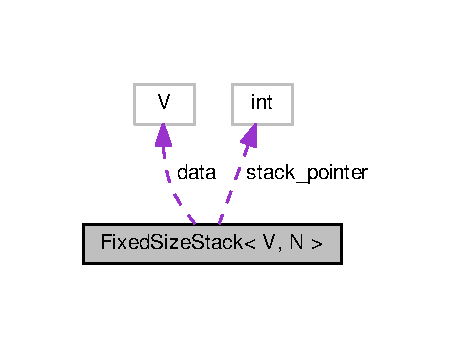
\includegraphics[width=217pt]{classFixedSizeStack__coll__graph}
\end{center}
\end{figure}
\subsection*{Public Member Functions}
\begin{DoxyCompactItemize}
\item 
\hyperlink{classFixedSizeStack_ab8090e6bfc34b69664fde6f7a9663071}{Fixed\+Size\+Stack} ()
\item 
void \hyperlink{classFixedSizeStack_a544e3fb119f4b93093db0f52b62bffb1}{pop} ()
\item 
V \hyperlink{classFixedSizeStack_a155565554dcbfade8363d3d6035613c5}{top} ()
\item 
bool \hyperlink{classFixedSizeStack_a9ec83cd2dc98e4a5145000da652bf112}{empty} () const 
\item 
void \hyperlink{classFixedSizeStack_abaa79c280f2ff9adb3ae919a0a8607fb}{push} (const V \&to\+\_\+push)
\item 
void \hyperlink{classFixedSizeStack_a62d9af2dd2c3d9e852a297483f4c4c50}{flush} ()
\end{DoxyCompactItemize}
\subsection*{Private Attributes}
\begin{DoxyCompactItemize}
\item 
int \hyperlink{classFixedSizeStack_a87e0a013c62888f127f57309e32ed70e}{stack\+\_\+pointer}
\item 
V \hyperlink{classFixedSizeStack_a25c7e307ab4079edafe72446c411aa74}{data} \mbox{[}N\mbox{]}
\end{DoxyCompactItemize}


\subsection{Detailed Description}
\subsubsection*{template$<$class V, unsigned int N$>$\\*
class Fixed\+Size\+Stack$<$ V, N $>$}

A stack that can contain at most N elements. If more are pushed to the stack, it will crash. No error handling is done. If top is called on an empty stack, it will crash. 


\begin{DoxyTemplParams}{Template Parameters}
{\em V} & Type of elements in the stack \\
\hline
{\em N} & Maximum number of elements in stack. \\
\hline
\end{DoxyTemplParams}


\subsection{Constructor \& Destructor Documentation}
\index{Fixed\+Size\+Stack@{Fixed\+Size\+Stack}!Fixed\+Size\+Stack@{Fixed\+Size\+Stack}}
\index{Fixed\+Size\+Stack@{Fixed\+Size\+Stack}!Fixed\+Size\+Stack@{Fixed\+Size\+Stack}}
\subsubsection[{\texorpdfstring{Fixed\+Size\+Stack()}{FixedSizeStack()}}]{\setlength{\rightskip}{0pt plus 5cm}template$<$class V , unsigned int N$>$ {\bf Fixed\+Size\+Stack}$<$ V, N $>$\+::{\bf Fixed\+Size\+Stack} (
\begin{DoxyParamCaption}
{}
\end{DoxyParamCaption}
)\hspace{0.3cm}{\ttfamily [inline]}}\hypertarget{classFixedSizeStack_ab8090e6bfc34b69664fde6f7a9663071}{}\label{classFixedSizeStack_ab8090e6bfc34b69664fde6f7a9663071}


\subsection{Member Function Documentation}
\index{Fixed\+Size\+Stack@{Fixed\+Size\+Stack}!empty@{empty}}
\index{empty@{empty}!Fixed\+Size\+Stack@{Fixed\+Size\+Stack}}
\subsubsection[{\texorpdfstring{empty() const }{empty() const }}]{\setlength{\rightskip}{0pt plus 5cm}template$<$class V , unsigned int N$>$ bool {\bf Fixed\+Size\+Stack}$<$ V, N $>$\+::empty (
\begin{DoxyParamCaption}
{}
\end{DoxyParamCaption}
) const\hspace{0.3cm}{\ttfamily [inline]}}\hypertarget{classFixedSizeStack_a9ec83cd2dc98e4a5145000da652bf112}{}\label{classFixedSizeStack_a9ec83cd2dc98e4a5145000da652bf112}
\index{Fixed\+Size\+Stack@{Fixed\+Size\+Stack}!flush@{flush}}
\index{flush@{flush}!Fixed\+Size\+Stack@{Fixed\+Size\+Stack}}
\subsubsection[{\texorpdfstring{flush()}{flush()}}]{\setlength{\rightskip}{0pt plus 5cm}template$<$class V , unsigned int N$>$ void {\bf Fixed\+Size\+Stack}$<$ V, N $>$\+::flush (
\begin{DoxyParamCaption}
{}
\end{DoxyParamCaption}
)\hspace{0.3cm}{\ttfamily [inline]}}\hypertarget{classFixedSizeStack_a62d9af2dd2c3d9e852a297483f4c4c50}{}\label{classFixedSizeStack_a62d9af2dd2c3d9e852a297483f4c4c50}
\index{Fixed\+Size\+Stack@{Fixed\+Size\+Stack}!pop@{pop}}
\index{pop@{pop}!Fixed\+Size\+Stack@{Fixed\+Size\+Stack}}
\subsubsection[{\texorpdfstring{pop()}{pop()}}]{\setlength{\rightskip}{0pt plus 5cm}template$<$class V , unsigned int N$>$ void {\bf Fixed\+Size\+Stack}$<$ V, N $>$\+::pop (
\begin{DoxyParamCaption}
{}
\end{DoxyParamCaption}
)\hspace{0.3cm}{\ttfamily [inline]}}\hypertarget{classFixedSizeStack_a544e3fb119f4b93093db0f52b62bffb1}{}\label{classFixedSizeStack_a544e3fb119f4b93093db0f52b62bffb1}
\index{Fixed\+Size\+Stack@{Fixed\+Size\+Stack}!push@{push}}
\index{push@{push}!Fixed\+Size\+Stack@{Fixed\+Size\+Stack}}
\subsubsection[{\texorpdfstring{push(const V \&to\+\_\+push)}{push(const V &to_push)}}]{\setlength{\rightskip}{0pt plus 5cm}template$<$class V , unsigned int N$>$ void {\bf Fixed\+Size\+Stack}$<$ V, N $>$\+::push (
\begin{DoxyParamCaption}
\item[{const V \&}]{to\+\_\+push}
\end{DoxyParamCaption}
)\hspace{0.3cm}{\ttfamily [inline]}}\hypertarget{classFixedSizeStack_abaa79c280f2ff9adb3ae919a0a8607fb}{}\label{classFixedSizeStack_abaa79c280f2ff9adb3ae919a0a8607fb}
\index{Fixed\+Size\+Stack@{Fixed\+Size\+Stack}!top@{top}}
\index{top@{top}!Fixed\+Size\+Stack@{Fixed\+Size\+Stack}}
\subsubsection[{\texorpdfstring{top()}{top()}}]{\setlength{\rightskip}{0pt plus 5cm}template$<$class V , unsigned int N$>$ V {\bf Fixed\+Size\+Stack}$<$ V, N $>$\+::top (
\begin{DoxyParamCaption}
{}
\end{DoxyParamCaption}
)\hspace{0.3cm}{\ttfamily [inline]}}\hypertarget{classFixedSizeStack_a155565554dcbfade8363d3d6035613c5}{}\label{classFixedSizeStack_a155565554dcbfade8363d3d6035613c5}


\subsection{Member Data Documentation}
\index{Fixed\+Size\+Stack@{Fixed\+Size\+Stack}!data@{data}}
\index{data@{data}!Fixed\+Size\+Stack@{Fixed\+Size\+Stack}}
\subsubsection[{\texorpdfstring{data}{data}}]{\setlength{\rightskip}{0pt plus 5cm}template$<$class V , unsigned int N$>$ V {\bf Fixed\+Size\+Stack}$<$ V, N $>$\+::data\mbox{[}N\mbox{]}\hspace{0.3cm}{\ttfamily [private]}}\hypertarget{classFixedSizeStack_a25c7e307ab4079edafe72446c411aa74}{}\label{classFixedSizeStack_a25c7e307ab4079edafe72446c411aa74}
\index{Fixed\+Size\+Stack@{Fixed\+Size\+Stack}!stack\+\_\+pointer@{stack\+\_\+pointer}}
\index{stack\+\_\+pointer@{stack\+\_\+pointer}!Fixed\+Size\+Stack@{Fixed\+Size\+Stack}}
\subsubsection[{\texorpdfstring{stack\+\_\+pointer}{stack_pointer}}]{\setlength{\rightskip}{0pt plus 5cm}template$<$class V , unsigned int N$>$ int {\bf Fixed\+Size\+Stack}$<$ V, N $>$\+::stack\+\_\+pointer\hspace{0.3cm}{\ttfamily [private]}}\hypertarget{classFixedSizeStack_a87e0a013c62888f127f57309e32ed70e}{}\label{classFixedSizeStack_a87e0a013c62888f127f57309e32ed70e}


The documentation for this class was generated from the following file\+:\begin{DoxyCompactItemize}
\item 
src/renderable/\hyperlink{BinaryVolumeHierarchy_8h}{Binary\+Volume\+Hierarchy.\+h}\end{DoxyCompactItemize}

\hypertarget{classImplicitSurface}{}\section{Implicit\+Surface Class Reference}
\label{classImplicitSurface}\index{Implicit\+Surface@{Implicit\+Surface}}


\hyperlink{classRenderObject}{Render\+Object} for the surface implicitly given by F(x,y,z) = 0.  




{\ttfamily \#include $<$Implicit\+Surface.\+h$>$}



Inheritance diagram for Implicit\+Surface\+:\nopagebreak
\begin{figure}[H]
\begin{center}
\leavevmode
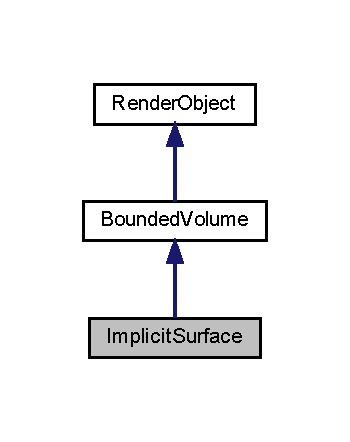
\includegraphics[width=168pt]{classImplicitSurface__inherit__graph}
\end{center}
\end{figure}


Collaboration diagram for Implicit\+Surface\+:\nopagebreak
\begin{figure}[H]
\begin{center}
\leavevmode
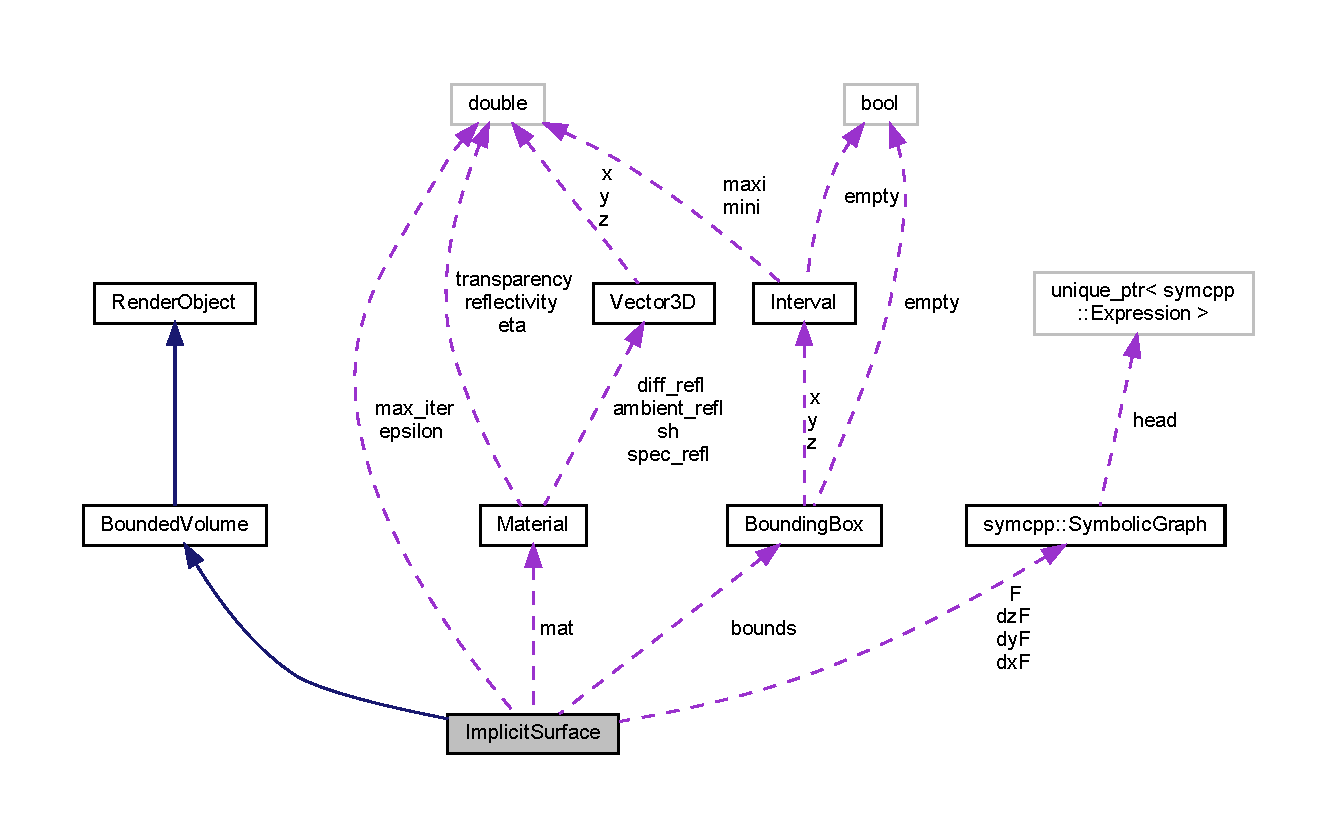
\includegraphics[width=350pt]{classImplicitSurface__coll__graph}
\end{center}
\end{figure}
\subsection*{Public Member Functions}
\begin{DoxyCompactItemize}
\item 
\hyperlink{classImplicitSurface_ab0cfa235e8f935a416c395cfecd2f32b}{Implicit\+Surface} (\hyperlink{classsymcpp_1_1SymbolicGraph}{symcpp\+::\+Symbolic\+Graph} f, \hyperlink{classMaterial}{Material} m, \hyperlink{classBoundingBox}{Bounding\+Box} b)
\item 
\hyperlink{classIntersection}{Intersection} \hyperlink{classImplicitSurface_a09b05170e1ff9d443c0c0ff9c33824f8}{ray\+Intersect} (const \hyperlink{classRay}{Ray} \&ray) const override
\begin{DoxyCompactList}\small\item\em Uses the symbolic derivative and the Newton method to detect the earliest intersection. \end{DoxyCompactList}\item 
\hyperlink{classIntersectionProperties}{Intersection\+Properties} \hyperlink{classImplicitSurface_a8ce29f3d491a01f1992a2ae534ee6bea}{intersect\+Properties} (const \hyperlink{classRay}{Ray} \&ray) const override
\begin{DoxyCompactList}\small\item\em If ray intersects this object, this method will provide additional Information. \end{DoxyCompactList}\item 
std\+::ostream \& \hyperlink{classImplicitSurface_a2267c88829c97c12ff8f7d250ce94802}{print} (std\+::ostream \&sink) const override
\item 
\hyperlink{classBoundingBox}{Bounding\+Box} \hyperlink{classImplicitSurface_a8fd17a82a612fc8d15c5973cb497c48b}{get\+Bounds} () const override
\end{DoxyCompactItemize}
\subsection*{Private Attributes}
\begin{DoxyCompactItemize}
\item 
\hyperlink{classsymcpp_1_1SymbolicGraph}{symcpp\+::\+Symbolic\+Graph} \hyperlink{classImplicitSurface_aeeafee33bf827627323373167ce841eb}{F}
\begin{DoxyCompactList}\small\item\em The function defining the surface by F(x, y, z) = 0. \end{DoxyCompactList}\item 
\hyperlink{classsymcpp_1_1SymbolicGraph}{symcpp\+::\+Symbolic\+Graph} \hyperlink{classImplicitSurface_a9861b92609a363bf78d73347a9272b5d}{dxF}
\begin{DoxyCompactList}\small\item\em The partial derivative by x. \end{DoxyCompactList}\item 
\hyperlink{classsymcpp_1_1SymbolicGraph}{symcpp\+::\+Symbolic\+Graph} \hyperlink{classImplicitSurface_a49145c0375f0adc02157b9368e733aa2}{dyF}
\begin{DoxyCompactList}\small\item\em The partial derivative by y. \end{DoxyCompactList}\item 
\hyperlink{classsymcpp_1_1SymbolicGraph}{symcpp\+::\+Symbolic\+Graph} \hyperlink{classImplicitSurface_aab31834ea321e276bb85348d7a7464f2}{dzF}
\begin{DoxyCompactList}\small\item\em The partial derivative by z. \end{DoxyCompactList}\item 
\hyperlink{classMaterial}{Material} \hyperlink{classImplicitSurface_adbb94dbb4d3271d5ed18752dde4aac32}{mat}
\item 
\hyperlink{classBoundingBox}{Bounding\+Box} \hyperlink{classImplicitSurface_a1332a4975d57ce5f91450221541df82a}{bounds}
\item 
double \hyperlink{classImplicitSurface_ad92c06925b2496b7fe3a1d2659a87075}{max\+\_\+iter}
\begin{DoxyCompactList}\small\item\em The maximum number of iterations in Newton method. \end{DoxyCompactList}\item 
double \hyperlink{classImplicitSurface_aa870a11380d4bc4c019d9d250e7ccc9c}{epsilon}
\end{DoxyCompactItemize}


\subsection{Detailed Description}
\hyperlink{classRenderObject}{Render\+Object} for the surface implicitly given by F(x,y,z) = 0. 

Objects of this type can be used to render meshless surfaces, eg manifolds. This is, however fairly slow. You might consider meshifying the object by applying the marching-\/cubes algorithm. 

\subsection{Constructor \& Destructor Documentation}
\index{Implicit\+Surface@{Implicit\+Surface}!Implicit\+Surface@{Implicit\+Surface}}
\index{Implicit\+Surface@{Implicit\+Surface}!Implicit\+Surface@{Implicit\+Surface}}
\subsubsection[{\texorpdfstring{Implicit\+Surface(symcpp\+::\+Symbolic\+Graph f, Material m, Bounding\+Box b)}{ImplicitSurface(symcpp::SymbolicGraph f, Material m, BoundingBox b)}}]{\setlength{\rightskip}{0pt plus 5cm}Implicit\+Surface\+::\+Implicit\+Surface (
\begin{DoxyParamCaption}
\item[{{\bf symcpp\+::\+Symbolic\+Graph}}]{f, }
\item[{{\bf Material}}]{m, }
\item[{{\bf Bounding\+Box}}]{b}
\end{DoxyParamCaption}
)}\hypertarget{classImplicitSurface_ab0cfa235e8f935a416c395cfecd2f32b}{}\label{classImplicitSurface_ab0cfa235e8f935a416c395cfecd2f32b}


\subsection{Member Function Documentation}
\index{Implicit\+Surface@{Implicit\+Surface}!get\+Bounds@{get\+Bounds}}
\index{get\+Bounds@{get\+Bounds}!Implicit\+Surface@{Implicit\+Surface}}
\subsubsection[{\texorpdfstring{get\+Bounds() const override}{getBounds() const override}}]{\setlength{\rightskip}{0pt plus 5cm}{\bf Bounding\+Box} Implicit\+Surface\+::get\+Bounds (
\begin{DoxyParamCaption}
{}
\end{DoxyParamCaption}
) const\hspace{0.3cm}{\ttfamily [override]}, {\ttfamily [virtual]}}\hypertarget{classImplicitSurface_a8fd17a82a612fc8d15c5973cb497c48b}{}\label{classImplicitSurface_a8fd17a82a612fc8d15c5973cb497c48b}


Implements \hyperlink{classBoundedVolume_a3d912b7028f7046fe18c4edf3a400e3b}{Bounded\+Volume}.

\index{Implicit\+Surface@{Implicit\+Surface}!intersect\+Properties@{intersect\+Properties}}
\index{intersect\+Properties@{intersect\+Properties}!Implicit\+Surface@{Implicit\+Surface}}
\subsubsection[{\texorpdfstring{intersect\+Properties(const Ray \&ray) const override}{intersectProperties(const Ray &ray) const override}}]{\setlength{\rightskip}{0pt plus 5cm}{\bf Intersection\+Properties} Implicit\+Surface\+::intersect\+Properties (
\begin{DoxyParamCaption}
\item[{const {\bf Ray} \&}]{ray}
\end{DoxyParamCaption}
) const\hspace{0.3cm}{\ttfamily [override]}, {\ttfamily [virtual]}}\hypertarget{classImplicitSurface_a8ce29f3d491a01f1992a2ae534ee6bea}{}\label{classImplicitSurface_a8ce29f3d491a01f1992a2ae534ee6bea}


If ray intersects this object, this method will provide additional Information. 

Note, that even if ray\+Intersect detected an intersection, this method might not be called. It is called iff the Intersection-\/\+Object returned by ray\+Intersect contains a pointer to this object and no other object in the rendered scene returned an intersection that was closer to the camera.


\begin{DoxyParams}{Parameters}
{\em ray} & the ray in question \\
\hline
\end{DoxyParams}
\begin{DoxyReturn}{Returns}
\hyperlink{classIntersectionProperties}{Intersection\+Properties} object containing the surface normal and material information 
\end{DoxyReturn}


Implements \hyperlink{classRenderObject_ae2c6d699741385dcd9ea6a1b09f9b7f0}{Render\+Object}.

\index{Implicit\+Surface@{Implicit\+Surface}!print@{print}}
\index{print@{print}!Implicit\+Surface@{Implicit\+Surface}}
\subsubsection[{\texorpdfstring{print(std\+::ostream \&sink) const override}{print(std::ostream &sink) const override}}]{\setlength{\rightskip}{0pt plus 5cm}std\+::ostream \& Implicit\+Surface\+::print (
\begin{DoxyParamCaption}
\item[{std\+::ostream \&}]{sink}
\end{DoxyParamCaption}
) const\hspace{0.3cm}{\ttfamily [override]}, {\ttfamily [virtual]}}\hypertarget{classImplicitSurface_a2267c88829c97c12ff8f7d250ce94802}{}\label{classImplicitSurface_a2267c88829c97c12ff8f7d250ce94802}


Implements \hyperlink{classRenderObject_a7a7f1168a7d96ca95235b170ff7fb11b}{Render\+Object}.

\index{Implicit\+Surface@{Implicit\+Surface}!ray\+Intersect@{ray\+Intersect}}
\index{ray\+Intersect@{ray\+Intersect}!Implicit\+Surface@{Implicit\+Surface}}
\subsubsection[{\texorpdfstring{ray\+Intersect(const Ray \&ray) const override}{rayIntersect(const Ray &ray) const override}}]{\setlength{\rightskip}{0pt plus 5cm}{\bf Intersection} Implicit\+Surface\+::ray\+Intersect (
\begin{DoxyParamCaption}
\item[{const {\bf Ray} \&}]{ray}
\end{DoxyParamCaption}
) const\hspace{0.3cm}{\ttfamily [override]}, {\ttfamily [virtual]}}\hypertarget{classImplicitSurface_a09b05170e1ff9d443c0c0ff9c33824f8}{}\label{classImplicitSurface_a09b05170e1ff9d443c0c0ff9c33824f8}


Uses the symbolic derivative and the Newton method to detect the earliest intersection. 

\begin{DoxySeeAlso}{See also}
\href{https://en.wikipedia.org/wiki/Newton%27s_method}{\tt https\+://en.\+wikipedia.\+org/wiki/\+Newton\%27s\+\_\+method} 
\end{DoxySeeAlso}

\begin{DoxyParams}{Parameters}
{\em ray} & The ray intersecting the surface \\
\hline
\end{DoxyParams}
\begin{DoxyReturn}{Returns}
\hyperlink{classIntersection}{Intersection} object containing distance of intersection and pointer to this 
\end{DoxyReturn}


Implements \hyperlink{classRenderObject_a681f6674d94f16c4df69605d5e42d05c}{Render\+Object}.



\subsection{Member Data Documentation}
\index{Implicit\+Surface@{Implicit\+Surface}!bounds@{bounds}}
\index{bounds@{bounds}!Implicit\+Surface@{Implicit\+Surface}}
\subsubsection[{\texorpdfstring{bounds}{bounds}}]{\setlength{\rightskip}{0pt plus 5cm}{\bf Bounding\+Box} Implicit\+Surface\+::bounds\hspace{0.3cm}{\ttfamily [private]}}\hypertarget{classImplicitSurface_a1332a4975d57ce5f91450221541df82a}{}\label{classImplicitSurface_a1332a4975d57ce5f91450221541df82a}
\index{Implicit\+Surface@{Implicit\+Surface}!dxF@{dxF}}
\index{dxF@{dxF}!Implicit\+Surface@{Implicit\+Surface}}
\subsubsection[{\texorpdfstring{dxF}{dxF}}]{\setlength{\rightskip}{0pt plus 5cm}{\bf symcpp\+::\+Symbolic\+Graph} Implicit\+Surface\+::dxF\hspace{0.3cm}{\ttfamily [private]}}\hypertarget{classImplicitSurface_a9861b92609a363bf78d73347a9272b5d}{}\label{classImplicitSurface_a9861b92609a363bf78d73347a9272b5d}


The partial derivative by x. 

\index{Implicit\+Surface@{Implicit\+Surface}!dyF@{dyF}}
\index{dyF@{dyF}!Implicit\+Surface@{Implicit\+Surface}}
\subsubsection[{\texorpdfstring{dyF}{dyF}}]{\setlength{\rightskip}{0pt plus 5cm}{\bf symcpp\+::\+Symbolic\+Graph} Implicit\+Surface\+::dyF\hspace{0.3cm}{\ttfamily [private]}}\hypertarget{classImplicitSurface_a49145c0375f0adc02157b9368e733aa2}{}\label{classImplicitSurface_a49145c0375f0adc02157b9368e733aa2}


The partial derivative by y. 

\index{Implicit\+Surface@{Implicit\+Surface}!dzF@{dzF}}
\index{dzF@{dzF}!Implicit\+Surface@{Implicit\+Surface}}
\subsubsection[{\texorpdfstring{dzF}{dzF}}]{\setlength{\rightskip}{0pt plus 5cm}symcpp\+:: Symbolic\+Graph Implicit\+Surface\+::dzF\hspace{0.3cm}{\ttfamily [private]}}\hypertarget{classImplicitSurface_aab31834ea321e276bb85348d7a7464f2}{}\label{classImplicitSurface_aab31834ea321e276bb85348d7a7464f2}


The partial derivative by z. 

\index{Implicit\+Surface@{Implicit\+Surface}!epsilon@{epsilon}}
\index{epsilon@{epsilon}!Implicit\+Surface@{Implicit\+Surface}}
\subsubsection[{\texorpdfstring{epsilon}{epsilon}}]{\setlength{\rightskip}{0pt plus 5cm}double Implicit\+Surface\+::epsilon\hspace{0.3cm}{\ttfamily [private]}}\hypertarget{classImplicitSurface_aa870a11380d4bc4c019d9d250e7ccc9c}{}\label{classImplicitSurface_aa870a11380d4bc4c019d9d250e7ccc9c}
\index{Implicit\+Surface@{Implicit\+Surface}!F@{F}}
\index{F@{F}!Implicit\+Surface@{Implicit\+Surface}}
\subsubsection[{\texorpdfstring{F}{F}}]{\setlength{\rightskip}{0pt plus 5cm}{\bf symcpp\+::\+Symbolic\+Graph} Implicit\+Surface\+::F\hspace{0.3cm}{\ttfamily [private]}}\hypertarget{classImplicitSurface_aeeafee33bf827627323373167ce841eb}{}\label{classImplicitSurface_aeeafee33bf827627323373167ce841eb}


The function defining the surface by F(x, y, z) = 0. 

\index{Implicit\+Surface@{Implicit\+Surface}!mat@{mat}}
\index{mat@{mat}!Implicit\+Surface@{Implicit\+Surface}}
\subsubsection[{\texorpdfstring{mat}{mat}}]{\setlength{\rightskip}{0pt plus 5cm}{\bf Material} Implicit\+Surface\+::mat\hspace{0.3cm}{\ttfamily [private]}}\hypertarget{classImplicitSurface_adbb94dbb4d3271d5ed18752dde4aac32}{}\label{classImplicitSurface_adbb94dbb4d3271d5ed18752dde4aac32}
\index{Implicit\+Surface@{Implicit\+Surface}!max\+\_\+iter@{max\+\_\+iter}}
\index{max\+\_\+iter@{max\+\_\+iter}!Implicit\+Surface@{Implicit\+Surface}}
\subsubsection[{\texorpdfstring{max\+\_\+iter}{max_iter}}]{\setlength{\rightskip}{0pt plus 5cm}double Implicit\+Surface\+::max\+\_\+iter\hspace{0.3cm}{\ttfamily [private]}}\hypertarget{classImplicitSurface_ad92c06925b2496b7fe3a1d2659a87075}{}\label{classImplicitSurface_ad92c06925b2496b7fe3a1d2659a87075}


The maximum number of iterations in Newton method. 



The documentation for this class was generated from the following files\+:\begin{DoxyCompactItemize}
\item 
src/\hyperlink{ImplicitSurface_8h}{Implicit\+Surface.\+h}\item 
src/\hyperlink{ImplicitSurface_8cpp}{Implicit\+Surface.\+cpp}\end{DoxyCompactItemize}

\hypertarget{classIntersection}{}\section{Intersection Class Reference}
\label{classIntersection}\index{Intersection@{Intersection}}


Class for storing information about intersection of a \hyperlink{classRay}{Ray} and a \hyperlink{classRenderObject}{Render\+Object}.  




{\ttfamily \#include $<$Intersection.\+h$>$}



Collaboration diagram for Intersection\+:\nopagebreak
\begin{figure}[H]
\begin{center}
\leavevmode
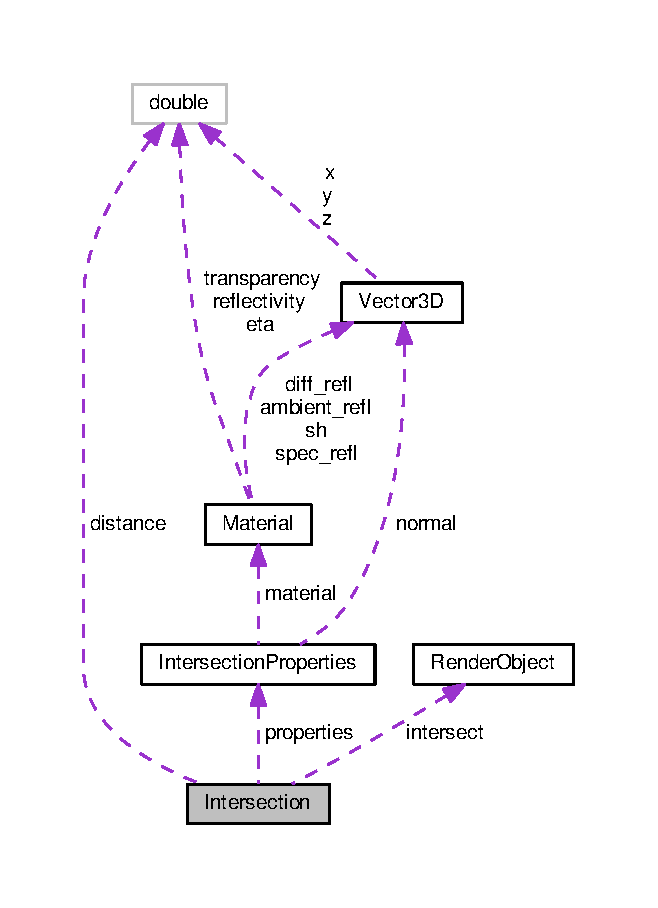
\includegraphics[width=316pt]{classIntersection__coll__graph}
\end{center}
\end{figure}
\subsection*{Public Member Functions}
\begin{DoxyCompactItemize}
\item 
\hyperlink{classIntersection_a6d6042fc104b258908c3c55d7cc23aa3}{Intersection} (const \hyperlink{classIntersection}{Intersection} \&other)
\item 
\hyperlink{classIntersection_accfff54844dea1b64fce8ddb1c72f84d}{Intersection} (const \hyperlink{classRenderObject}{Render\+Object} $\ast$\hyperlink{classIntersection_a8241676dd0f240769dc189132dc3c5bb}{intersect}, const double \&d)
\item 
\hyperlink{classIntersection_a8c9336839207202dbd7cc8eef633272e}{Intersection} (const \hyperlink{classRenderObject}{Render\+Object} $\ast$\hyperlink{classIntersection_a8241676dd0f240769dc189132dc3c5bb}{intersect}, const double \&d, const \hyperlink{classIntersectionProperties}{Intersection\+Properties} \&p)
\item 
\hyperlink{classIntersection_a67497e3efe2793b23909052eeb82c4f3}{Intersection} ()
\item 
bool \hyperlink{classIntersection_ae2d6edc03a6a048258724c2ca7ca2dc8}{does\+\_\+intersect} ()
\item 
double \hyperlink{classIntersection_a3ebb19b50063f6034a36a1d59ae2f483}{get\+\_\+distance} () const 
\item 
void \hyperlink{classIntersection_afeb53190b4cae138c2ab89b8b7198481}{set\+\_\+properties} (const \hyperlink{classIntersectionProperties}{Intersection\+Properties} \&p)
\begin{DoxyCompactList}\small\item\em \hyperlink{classRenderObject}{Render\+Object} might choose to store information about the intersection here. \end{DoxyCompactList}\item 
void \hyperlink{classIntersection_aa5b98f38c76a5b3fb869b89ddc77f2da}{set\+\_\+properties} (const \hyperlink{classMaterial}{Material} \&mat, const \hyperlink{classVector3D}{Vector3D} \&normal)
\begin{DoxyCompactList}\small\item\em \hyperlink{classRenderObject}{Render\+Object} might choose to store information about the intersection here. \end{DoxyCompactList}\item 
bool \hyperlink{classIntersection_a5315f78b43c5ec261497bf87003d0613}{has\+\_\+properties} () const 
\item 
\hyperlink{classIntersectionProperties}{Intersection\+Properties} \hyperlink{classIntersection_ada64d34f2099bd8436978c7dacf05f32}{get\+\_\+properties} () const 
\begin{DoxyCompactList}\small\item\em Returns \hyperlink{classIntersectionProperties}{Intersection\+Properties} if they are stored here. Otherwise this method throws an exception. \end{DoxyCompactList}\item 
const \hyperlink{classRenderObject}{Render\+Object} $\ast$ \hyperlink{classIntersection_ae2047415852535497e951e8a98deaffb}{get\+\_\+object} () const 
\item 
\hyperlink{classIntersection}{Intersection} \& \hyperlink{classIntersection_add5b6d995062799bd840c6486790c604}{operator=} (const \hyperlink{classIntersection}{Intersection} \&other)
\item 
\hyperlink{classIntersection_a064951a970ed8dd11081b2903ab62122}{$\sim$\+Intersection} ()
\begin{DoxyCompactList}\small\item\em Destructor of \hyperlink{classIntersection}{Intersection}. \end{DoxyCompactList}\end{DoxyCompactItemize}
\subsection*{Private Attributes}
\begin{DoxyCompactItemize}
\item 
const \hyperlink{classRenderObject}{Render\+Object} $\ast$ \hyperlink{classIntersection_a8241676dd0f240769dc189132dc3c5bb}{intersect}
\item 
\hyperlink{classIntersectionProperties}{Intersection\+Properties} $\ast$ \hyperlink{classIntersection_ad9d38892c2e47f51ae2497904050c00e}{properties}
\item 
double \hyperlink{classIntersection_a65da854f067b6f08175a97d262a17f1e}{distance}
\end{DoxyCompactItemize}
\subsection*{Friends}
\begin{DoxyCompactItemize}
\item 
bool \hyperlink{classIntersection_a955ab59fdb5154881d491eebc653250f}{operator$<$} (const \hyperlink{classIntersection}{Intersection} \&first, const \hyperlink{classIntersection}{Intersection} \&second)
\begin{DoxyCompactList}\small\item\em Decides which intersection is closer to the camera. \end{DoxyCompactList}\end{DoxyCompactItemize}


\subsection{Detailed Description}
Class for storing information about intersection of a \hyperlink{classRay}{Ray} and a \hyperlink{classRenderObject}{Render\+Object}. 

\subsection{Constructor \& Destructor Documentation}
\index{Intersection@{Intersection}!Intersection@{Intersection}}
\index{Intersection@{Intersection}!Intersection@{Intersection}}
\subsubsection[{\texorpdfstring{Intersection(const Intersection \&other)}{Intersection(const Intersection &other)}}]{\setlength{\rightskip}{0pt plus 5cm}Intersection\+::\+Intersection (
\begin{DoxyParamCaption}
\item[{const {\bf Intersection} \&}]{other}
\end{DoxyParamCaption}
)}\hypertarget{classIntersection_a6d6042fc104b258908c3c55d7cc23aa3}{}\label{classIntersection_a6d6042fc104b258908c3c55d7cc23aa3}
\index{Intersection@{Intersection}!Intersection@{Intersection}}
\index{Intersection@{Intersection}!Intersection@{Intersection}}
\subsubsection[{\texorpdfstring{Intersection(const Render\+Object $\ast$intersect, const double \&d)}{Intersection(const RenderObject *intersect, const double &d)}}]{\setlength{\rightskip}{0pt plus 5cm}Intersection\+::\+Intersection (
\begin{DoxyParamCaption}
\item[{const {\bf Render\+Object} $\ast$}]{intersect, }
\item[{const double \&}]{d}
\end{DoxyParamCaption}
)}\hypertarget{classIntersection_accfff54844dea1b64fce8ddb1c72f84d}{}\label{classIntersection_accfff54844dea1b64fce8ddb1c72f84d}
\index{Intersection@{Intersection}!Intersection@{Intersection}}
\index{Intersection@{Intersection}!Intersection@{Intersection}}
\subsubsection[{\texorpdfstring{Intersection(const Render\+Object $\ast$intersect, const double \&d, const Intersection\+Properties \&p)}{Intersection(const RenderObject *intersect, const double &d, const IntersectionProperties &p)}}]{\setlength{\rightskip}{0pt plus 5cm}Intersection\+::\+Intersection (
\begin{DoxyParamCaption}
\item[{const {\bf Render\+Object} $\ast$}]{intersect, }
\item[{const double \&}]{d, }
\item[{const {\bf Intersection\+Properties} \&}]{p}
\end{DoxyParamCaption}
)}\hypertarget{classIntersection_a8c9336839207202dbd7cc8eef633272e}{}\label{classIntersection_a8c9336839207202dbd7cc8eef633272e}
\index{Intersection@{Intersection}!Intersection@{Intersection}}
\index{Intersection@{Intersection}!Intersection@{Intersection}}
\subsubsection[{\texorpdfstring{Intersection()}{Intersection()}}]{\setlength{\rightskip}{0pt plus 5cm}Intersection\+::\+Intersection (
\begin{DoxyParamCaption}
{}
\end{DoxyParamCaption}
)}\hypertarget{classIntersection_a67497e3efe2793b23909052eeb82c4f3}{}\label{classIntersection_a67497e3efe2793b23909052eeb82c4f3}
\index{Intersection@{Intersection}!````~Intersection@{$\sim$\+Intersection}}
\index{````~Intersection@{$\sim$\+Intersection}!Intersection@{Intersection}}
\subsubsection[{\texorpdfstring{$\sim$\+Intersection()}{~Intersection()}}]{\setlength{\rightskip}{0pt plus 5cm}Intersection\+::$\sim$\+Intersection (
\begin{DoxyParamCaption}
{}
\end{DoxyParamCaption}
)}\hypertarget{classIntersection_a064951a970ed8dd11081b2903ab62122}{}\label{classIntersection_a064951a970ed8dd11081b2903ab62122}


Destructor of \hyperlink{classIntersection}{Intersection}. 

Note, that we only have to delete properties. It is not \hyperlink{classIntersection}{Intersection}\textquotesingle{}s responsibility to clean up intersect. In fact, chances are intersect is not even on the heap. 

\subsection{Member Function Documentation}
\index{Intersection@{Intersection}!does\+\_\+intersect@{does\+\_\+intersect}}
\index{does\+\_\+intersect@{does\+\_\+intersect}!Intersection@{Intersection}}
\subsubsection[{\texorpdfstring{does\+\_\+intersect()}{does_intersect()}}]{\setlength{\rightskip}{0pt plus 5cm}bool Intersection\+::does\+\_\+intersect (
\begin{DoxyParamCaption}
{}
\end{DoxyParamCaption}
)}\hypertarget{classIntersection_ae2d6edc03a6a048258724c2ca7ca2dc8}{}\label{classIntersection_ae2d6edc03a6a048258724c2ca7ca2dc8}
\index{Intersection@{Intersection}!get\+\_\+distance@{get\+\_\+distance}}
\index{get\+\_\+distance@{get\+\_\+distance}!Intersection@{Intersection}}
\subsubsection[{\texorpdfstring{get\+\_\+distance() const }{get_distance() const }}]{\setlength{\rightskip}{0pt plus 5cm}double Intersection\+::get\+\_\+distance (
\begin{DoxyParamCaption}
{}
\end{DoxyParamCaption}
) const}\hypertarget{classIntersection_a3ebb19b50063f6034a36a1d59ae2f483}{}\label{classIntersection_a3ebb19b50063f6034a36a1d59ae2f483}
\index{Intersection@{Intersection}!get\+\_\+object@{get\+\_\+object}}
\index{get\+\_\+object@{get\+\_\+object}!Intersection@{Intersection}}
\subsubsection[{\texorpdfstring{get\+\_\+object() const }{get_object() const }}]{\setlength{\rightskip}{0pt plus 5cm}const {\bf Render\+Object} $\ast$ Intersection\+::get\+\_\+object (
\begin{DoxyParamCaption}
{}
\end{DoxyParamCaption}
) const}\hypertarget{classIntersection_ae2047415852535497e951e8a98deaffb}{}\label{classIntersection_ae2047415852535497e951e8a98deaffb}
\index{Intersection@{Intersection}!get\+\_\+properties@{get\+\_\+properties}}
\index{get\+\_\+properties@{get\+\_\+properties}!Intersection@{Intersection}}
\subsubsection[{\texorpdfstring{get\+\_\+properties() const }{get_properties() const }}]{\setlength{\rightskip}{0pt plus 5cm}{\bf Intersection\+Properties} Intersection\+::get\+\_\+properties (
\begin{DoxyParamCaption}
{}
\end{DoxyParamCaption}
) const}\hypertarget{classIntersection_ada64d34f2099bd8436978c7dacf05f32}{}\label{classIntersection_ada64d34f2099bd8436978c7dacf05f32}


Returns \hyperlink{classIntersectionProperties}{Intersection\+Properties} if they are stored here. Otherwise this method throws an exception. 

Before calling this method you might want to call has\+\_\+properties \begin{DoxyReturn}{Returns}
Information about the intersection if these properties were stored here 
\end{DoxyReturn}
\index{Intersection@{Intersection}!has\+\_\+properties@{has\+\_\+properties}}
\index{has\+\_\+properties@{has\+\_\+properties}!Intersection@{Intersection}}
\subsubsection[{\texorpdfstring{has\+\_\+properties() const }{has_properties() const }}]{\setlength{\rightskip}{0pt plus 5cm}bool Intersection\+::has\+\_\+properties (
\begin{DoxyParamCaption}
{}
\end{DoxyParamCaption}
) const}\hypertarget{classIntersection_a5315f78b43c5ec261497bf87003d0613}{}\label{classIntersection_a5315f78b43c5ec261497bf87003d0613}
\begin{DoxyReturn}{Returns}
True if information about intersection properties are stored in this object 
\end{DoxyReturn}
\index{Intersection@{Intersection}!operator=@{operator=}}
\index{operator=@{operator=}!Intersection@{Intersection}}
\subsubsection[{\texorpdfstring{operator=(const Intersection \&other)}{operator=(const Intersection &other)}}]{\setlength{\rightskip}{0pt plus 5cm}{\bf Intersection} \& Intersection\+::operator= (
\begin{DoxyParamCaption}
\item[{const {\bf Intersection} \&}]{other}
\end{DoxyParamCaption}
)}\hypertarget{classIntersection_add5b6d995062799bd840c6486790c604}{}\label{classIntersection_add5b6d995062799bd840c6486790c604}
\index{Intersection@{Intersection}!set\+\_\+properties@{set\+\_\+properties}}
\index{set\+\_\+properties@{set\+\_\+properties}!Intersection@{Intersection}}
\subsubsection[{\texorpdfstring{set\+\_\+properties(const Intersection\+Properties \&p)}{set_properties(const IntersectionProperties &p)}}]{\setlength{\rightskip}{0pt plus 5cm}void Intersection\+::set\+\_\+properties (
\begin{DoxyParamCaption}
\item[{const {\bf Intersection\+Properties} \&}]{p}
\end{DoxyParamCaption}
)}\hypertarget{classIntersection_afeb53190b4cae138c2ab89b8b7198481}{}\label{classIntersection_afeb53190b4cae138c2ab89b8b7198481}


\hyperlink{classRenderObject}{Render\+Object} might choose to store information about the intersection here. 


\begin{DoxyParams}{Parameters}
{\em p} & Properties of the intersection \\
\hline
\end{DoxyParams}
\index{Intersection@{Intersection}!set\+\_\+properties@{set\+\_\+properties}}
\index{set\+\_\+properties@{set\+\_\+properties}!Intersection@{Intersection}}
\subsubsection[{\texorpdfstring{set\+\_\+properties(const Material \&mat, const Vector3\+D \&normal)}{set_properties(const Material &mat, const Vector3D &normal)}}]{\setlength{\rightskip}{0pt plus 5cm}void Intersection\+::set\+\_\+properties (
\begin{DoxyParamCaption}
\item[{const {\bf Material} \&}]{mat, }
\item[{const {\bf Vector3D} \&}]{normal}
\end{DoxyParamCaption}
)}\hypertarget{classIntersection_aa5b98f38c76a5b3fb869b89ddc77f2da}{}\label{classIntersection_aa5b98f38c76a5b3fb869b89ddc77f2da}


\hyperlink{classRenderObject}{Render\+Object} might choose to store information about the intersection here. 

Setting the properties using this method will allow \hyperlink{classScene}{Scene} to avoid calling intersect\+\_\+properties of Renderobject. This might be desired if the surface normal/materials are calculated by Render\+Objects ray\+\_\+intersect already. 
\begin{DoxyParams}{Parameters}
{\em mat} & The material properties at the intersection point \\
\hline
{\em normal} & The surface normal at the intersection point \\
\hline
\end{DoxyParams}


\subsection{Friends And Related Function Documentation}
\index{Intersection@{Intersection}!operator$<$@{operator$<$}}
\index{operator$<$@{operator$<$}!Intersection@{Intersection}}
\subsubsection[{\texorpdfstring{operator$<$}{operator<}}]{\setlength{\rightskip}{0pt plus 5cm}bool operator$<$ (
\begin{DoxyParamCaption}
\item[{const {\bf Intersection} \&}]{first, }
\item[{const {\bf Intersection} \&}]{second}
\end{DoxyParamCaption}
)\hspace{0.3cm}{\ttfamily [friend]}}\hypertarget{classIntersection_a955ab59fdb5154881d491eebc653250f}{}\label{classIntersection_a955ab59fdb5154881d491eebc653250f}


Decides which intersection is closer to the camera. 


\begin{DoxyParams}{Parameters}
{\em first} & The first intersection \\
\hline
{\em second} & The second intersection \\
\hline
\end{DoxyParams}
\begin{DoxyReturn}{Returns}
True if first is closer to the camera than second 
\end{DoxyReturn}


\subsection{Member Data Documentation}
\index{Intersection@{Intersection}!distance@{distance}}
\index{distance@{distance}!Intersection@{Intersection}}
\subsubsection[{\texorpdfstring{distance}{distance}}]{\setlength{\rightskip}{0pt plus 5cm}double Intersection\+::distance\hspace{0.3cm}{\ttfamily [private]}}\hypertarget{classIntersection_a65da854f067b6f08175a97d262a17f1e}{}\label{classIntersection_a65da854f067b6f08175a97d262a17f1e}
\index{Intersection@{Intersection}!intersect@{intersect}}
\index{intersect@{intersect}!Intersection@{Intersection}}
\subsubsection[{\texorpdfstring{intersect}{intersect}}]{\setlength{\rightskip}{0pt plus 5cm}const {\bf Render\+Object}$\ast$ Intersection\+::intersect\hspace{0.3cm}{\ttfamily [private]}}\hypertarget{classIntersection_a8241676dd0f240769dc189132dc3c5bb}{}\label{classIntersection_a8241676dd0f240769dc189132dc3c5bb}
\index{Intersection@{Intersection}!properties@{properties}}
\index{properties@{properties}!Intersection@{Intersection}}
\subsubsection[{\texorpdfstring{properties}{properties}}]{\setlength{\rightskip}{0pt plus 5cm}{\bf Intersection\+Properties}$\ast$ Intersection\+::properties\hspace{0.3cm}{\ttfamily [private]}}\hypertarget{classIntersection_ad9d38892c2e47f51ae2497904050c00e}{}\label{classIntersection_ad9d38892c2e47f51ae2497904050c00e}


The documentation for this class was generated from the following files\+:\begin{DoxyCompactItemize}
\item 
src/\hyperlink{Intersection_8h}{Intersection.\+h}\item 
src/\hyperlink{Intersection_8cpp}{Intersection.\+cpp}\end{DoxyCompactItemize}

\hypertarget{classIntersectionProperties}{}\section{Intersection\+Properties Class Reference}
\label{classIntersectionProperties}\index{IntersectionProperties@{IntersectionProperties}}


Class for storing information about the local properties of a \mbox{\hyperlink{classRenderObject}{Render\+Object}} at a specific point in space.  




{\ttfamily \#include $<$Intersection\+Properties.\+h$>$}



Collaboration diagram for Intersection\+Properties\+:
\nopagebreak
\begin{figure}[H]
\begin{center}
\leavevmode
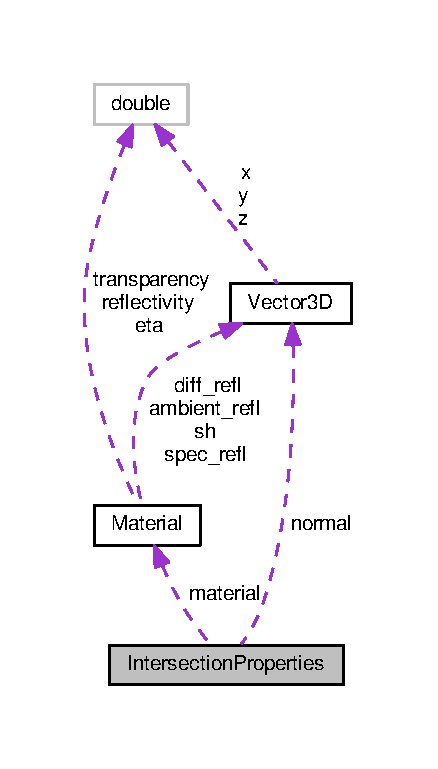
\includegraphics[width=224pt]{classIntersectionProperties__coll__graph}
\end{center}
\end{figure}
\subsection*{Public Member Functions}
\begin{DoxyCompactItemize}
\item 
\mbox{\hyperlink{classIntersectionProperties_af6f71f18a350a95cfab225d5f13be280}{Intersection\+Properties}} ()=default
\item 
\mbox{\hyperlink{classIntersectionProperties_a375cfefda4657bdc278504213347bde8}{Intersection\+Properties}} (const \mbox{\hyperlink{classVector3D}{Vector3D}} \&n, const \mbox{\hyperlink{classMaterial}{Material}} \&mat)
\end{DoxyCompactItemize}
\subsection*{Public Attributes}
\begin{DoxyCompactItemize}
\item 
\mbox{\hyperlink{classVector3D}{Vector3D}} \mbox{\hyperlink{classIntersectionProperties_afb99c699b3116580c68936d033b09081}{normal}}
\item 
\mbox{\hyperlink{classMaterial}{Material}} \mbox{\hyperlink{classIntersectionProperties_a52218ae741a9cd035eeed6cbc40b3300}{material}}
\end{DoxyCompactItemize}


\subsection{Detailed Description}
Class for storing information about the local properties of a \mbox{\hyperlink{classRenderObject}{Render\+Object}} at a specific point in space. 

\subsection{Constructor \& Destructor Documentation}
\mbox{\Hypertarget{classIntersectionProperties_af6f71f18a350a95cfab225d5f13be280}\label{classIntersectionProperties_af6f71f18a350a95cfab225d5f13be280}} 
\index{IntersectionProperties@{IntersectionProperties}!IntersectionProperties@{IntersectionProperties}}
\index{IntersectionProperties@{IntersectionProperties}!IntersectionProperties@{IntersectionProperties}}
\subsubsection{\texorpdfstring{IntersectionProperties()}{IntersectionProperties()}\hspace{0.1cm}{\footnotesize\ttfamily [1/2]}}
{\footnotesize\ttfamily Intersection\+Properties\+::\+Intersection\+Properties (\begin{DoxyParamCaption}{ }\end{DoxyParamCaption})\hspace{0.3cm}{\ttfamily [default]}}

\mbox{\Hypertarget{classIntersectionProperties_a375cfefda4657bdc278504213347bde8}\label{classIntersectionProperties_a375cfefda4657bdc278504213347bde8}} 
\index{IntersectionProperties@{IntersectionProperties}!IntersectionProperties@{IntersectionProperties}}
\index{IntersectionProperties@{IntersectionProperties}!IntersectionProperties@{IntersectionProperties}}
\subsubsection{\texorpdfstring{IntersectionProperties()}{IntersectionProperties()}\hspace{0.1cm}{\footnotesize\ttfamily [2/2]}}
{\footnotesize\ttfamily Intersection\+Properties\+::\+Intersection\+Properties (\begin{DoxyParamCaption}\item[{const \mbox{\hyperlink{classVector3D}{Vector3D}} \&}]{n,  }\item[{const \mbox{\hyperlink{classMaterial}{Material}} \&}]{mat }\end{DoxyParamCaption})}



\subsection{Member Data Documentation}
\mbox{\Hypertarget{classIntersectionProperties_a52218ae741a9cd035eeed6cbc40b3300}\label{classIntersectionProperties_a52218ae741a9cd035eeed6cbc40b3300}} 
\index{IntersectionProperties@{IntersectionProperties}!material@{material}}
\index{material@{material}!IntersectionProperties@{IntersectionProperties}}
\subsubsection{\texorpdfstring{material}{material}}
{\footnotesize\ttfamily \mbox{\hyperlink{classMaterial}{Material}} Intersection\+Properties\+::material}

\mbox{\Hypertarget{classIntersectionProperties_afb99c699b3116580c68936d033b09081}\label{classIntersectionProperties_afb99c699b3116580c68936d033b09081}} 
\index{IntersectionProperties@{IntersectionProperties}!normal@{normal}}
\index{normal@{normal}!IntersectionProperties@{IntersectionProperties}}
\subsubsection{\texorpdfstring{normal}{normal}}
{\footnotesize\ttfamily \mbox{\hyperlink{classVector3D}{Vector3D}} Intersection\+Properties\+::normal}



The documentation for this class was generated from the following files\+:\begin{DoxyCompactItemize}
\item 
src/\mbox{\hyperlink{IntersectionProperties_8h}{Intersection\+Properties.\+h}}\item 
src/\mbox{\hyperlink{IntersectionProperties_8cpp}{Intersection\+Properties.\+cpp}}\end{DoxyCompactItemize}

\hypertarget{classInterval}{}\section{Interval Class Reference}
\label{classInterval}\index{Interval@{Interval}}


The closed interval \mbox{[}mini, maxi\mbox{]}.  




{\ttfamily \#include $<$Interval.\+h$>$}



Collaboration diagram for Interval\+:\nopagebreak
\begin{figure}[H]
\begin{center}
\leavevmode
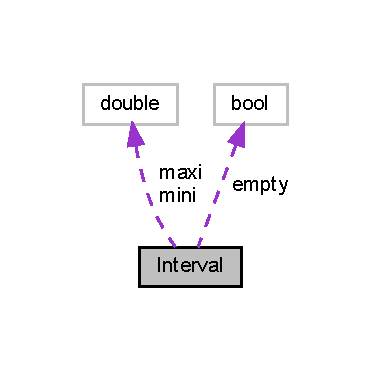
\includegraphics[width=180pt]{classInterval__coll__graph}
\end{center}
\end{figure}
\subsection*{Public Member Functions}
\begin{DoxyCompactItemize}
\item 
\hyperlink{classInterval_ab0a8f191fb00803d529902f85524e4e2}{Interval} (double min, double max)
\item 
\hyperlink{classInterval_ae48b9a9e9f672f81977627b609e32429}{Interval} ()
\item 
\hyperlink{classInterval}{Interval} \hyperlink{classInterval_a0c42da82e278c84a85a356b5ada6d4f4}{operator+} (const \hyperlink{classInterval}{Interval} \&other) const 
\item 
double \hyperlink{classInterval_a5b6e9f412603b80fd1ca427f6943d993}{mid\+Point} () const 
\item 
\hyperlink{classInterval}{Interval} \hyperlink{classInterval_a7098e87f0ffd13735a06060b0bd6b193}{operator$\ast$} (const \hyperlink{classInterval}{Interval} \&other) const 
\item 
bool \hyperlink{classInterval_a35d360b096b1551e328a25450cde5f72}{is\+Empty} () const 
\item 
bool \hyperlink{classInterval_a34d1acaf0a9b8d273dcbe48280f76894}{contains\+Positive} () const 
\item 
bool \hyperlink{classInterval_a8f1381466a2ed75a6487a92835cf20a8}{contains} (double x) const 
\item 
double \hyperlink{classInterval_aa90ef0b9050beabffcc789c3877cddd0}{get\+Min} () const 
\item 
double \hyperlink{classInterval_ab2fb3df4bc312013c19d54466d9d6470}{get\+Max} () const 
\item 
double \hyperlink{classInterval_ad502b7f22eb07d9ebba23cc9af869487}{get\+Center} () const 
\item 
double \hyperlink{classInterval_ad8cc11adfccd0e30ff3d93ad6a8b5a47}{length} () const 
\end{DoxyCompactItemize}
\subsection*{Private Attributes}
\begin{DoxyCompactItemize}
\item 
double \hyperlink{classInterval_aeb6ee750751e32a0f92d23f0a44ab122}{mini}
\item 
double \hyperlink{classInterval_ac086c91ab2c6f75ce8b3ff3818b38798}{maxi}
\item 
bool \hyperlink{classInterval_a9d9385e1ce6637e5760d26bf80aeada6}{empty}
\end{DoxyCompactItemize}
\subsection*{Friends}
\begin{DoxyCompactItemize}
\item 
std\+::ostream \& \hyperlink{classInterval_a7057e2823f722cd67f45b53382173b9f}{operator$<$$<$} (std\+::ostream \&sink, const \hyperlink{classInterval}{Interval} \&i)
\end{DoxyCompactItemize}


\subsection{Detailed Description}
The closed interval \mbox{[}mini, maxi\mbox{]}. 

\subsection{Constructor \& Destructor Documentation}
\index{Interval@{Interval}!Interval@{Interval}}
\index{Interval@{Interval}!Interval@{Interval}}
\subsubsection[{\texorpdfstring{Interval(double min, double max)}{Interval(double min, double max)}}]{\setlength{\rightskip}{0pt plus 5cm}Interval\+::\+Interval (
\begin{DoxyParamCaption}
\item[{double}]{min, }
\item[{double}]{max}
\end{DoxyParamCaption}
)}\hypertarget{classInterval_ab0a8f191fb00803d529902f85524e4e2}{}\label{classInterval_ab0a8f191fb00803d529902f85524e4e2}
\index{Interval@{Interval}!Interval@{Interval}}
\index{Interval@{Interval}!Interval@{Interval}}
\subsubsection[{\texorpdfstring{Interval()}{Interval()}}]{\setlength{\rightskip}{0pt plus 5cm}Interval\+::\+Interval (
\begin{DoxyParamCaption}
{}
\end{DoxyParamCaption}
)}\hypertarget{classInterval_ae48b9a9e9f672f81977627b609e32429}{}\label{classInterval_ae48b9a9e9f672f81977627b609e32429}


\subsection{Member Function Documentation}
\index{Interval@{Interval}!contains@{contains}}
\index{contains@{contains}!Interval@{Interval}}
\subsubsection[{\texorpdfstring{contains(double x) const }{contains(double x) const }}]{\setlength{\rightskip}{0pt plus 5cm}bool Interval\+::contains (
\begin{DoxyParamCaption}
\item[{double}]{x}
\end{DoxyParamCaption}
) const}\hypertarget{classInterval_a8f1381466a2ed75a6487a92835cf20a8}{}\label{classInterval_a8f1381466a2ed75a6487a92835cf20a8}
\index{Interval@{Interval}!contains\+Positive@{contains\+Positive}}
\index{contains\+Positive@{contains\+Positive}!Interval@{Interval}}
\subsubsection[{\texorpdfstring{contains\+Positive() const }{containsPositive() const }}]{\setlength{\rightskip}{0pt plus 5cm}bool Interval\+::contains\+Positive (
\begin{DoxyParamCaption}
{}
\end{DoxyParamCaption}
) const}\hypertarget{classInterval_a34d1acaf0a9b8d273dcbe48280f76894}{}\label{classInterval_a34d1acaf0a9b8d273dcbe48280f76894}
\index{Interval@{Interval}!get\+Center@{get\+Center}}
\index{get\+Center@{get\+Center}!Interval@{Interval}}
\subsubsection[{\texorpdfstring{get\+Center() const }{getCenter() const }}]{\setlength{\rightskip}{0pt plus 5cm}double Interval\+::get\+Center (
\begin{DoxyParamCaption}
{}
\end{DoxyParamCaption}
) const}\hypertarget{classInterval_ad502b7f22eb07d9ebba23cc9af869487}{}\label{classInterval_ad502b7f22eb07d9ebba23cc9af869487}
\index{Interval@{Interval}!get\+Max@{get\+Max}}
\index{get\+Max@{get\+Max}!Interval@{Interval}}
\subsubsection[{\texorpdfstring{get\+Max() const }{getMax() const }}]{\setlength{\rightskip}{0pt plus 5cm}double Interval\+::get\+Max (
\begin{DoxyParamCaption}
{}
\end{DoxyParamCaption}
) const}\hypertarget{classInterval_ab2fb3df4bc312013c19d54466d9d6470}{}\label{classInterval_ab2fb3df4bc312013c19d54466d9d6470}
\index{Interval@{Interval}!get\+Min@{get\+Min}}
\index{get\+Min@{get\+Min}!Interval@{Interval}}
\subsubsection[{\texorpdfstring{get\+Min() const }{getMin() const }}]{\setlength{\rightskip}{0pt plus 5cm}double Interval\+::get\+Min (
\begin{DoxyParamCaption}
{}
\end{DoxyParamCaption}
) const}\hypertarget{classInterval_aa90ef0b9050beabffcc789c3877cddd0}{}\label{classInterval_aa90ef0b9050beabffcc789c3877cddd0}
\index{Interval@{Interval}!is\+Empty@{is\+Empty}}
\index{is\+Empty@{is\+Empty}!Interval@{Interval}}
\subsubsection[{\texorpdfstring{is\+Empty() const }{isEmpty() const }}]{\setlength{\rightskip}{0pt plus 5cm}bool Interval\+::is\+Empty (
\begin{DoxyParamCaption}
{}
\end{DoxyParamCaption}
) const}\hypertarget{classInterval_a35d360b096b1551e328a25450cde5f72}{}\label{classInterval_a35d360b096b1551e328a25450cde5f72}
\index{Interval@{Interval}!length@{length}}
\index{length@{length}!Interval@{Interval}}
\subsubsection[{\texorpdfstring{length() const }{length() const }}]{\setlength{\rightskip}{0pt plus 5cm}double Interval\+::length (
\begin{DoxyParamCaption}
{}
\end{DoxyParamCaption}
) const}\hypertarget{classInterval_ad8cc11adfccd0e30ff3d93ad6a8b5a47}{}\label{classInterval_ad8cc11adfccd0e30ff3d93ad6a8b5a47}
\index{Interval@{Interval}!mid\+Point@{mid\+Point}}
\index{mid\+Point@{mid\+Point}!Interval@{Interval}}
\subsubsection[{\texorpdfstring{mid\+Point() const }{midPoint() const }}]{\setlength{\rightskip}{0pt plus 5cm}double Interval\+::mid\+Point (
\begin{DoxyParamCaption}
{}
\end{DoxyParamCaption}
) const}\hypertarget{classInterval_a5b6e9f412603b80fd1ca427f6943d993}{}\label{classInterval_a5b6e9f412603b80fd1ca427f6943d993}
\index{Interval@{Interval}!operator$\ast$@{operator$\ast$}}
\index{operator$\ast$@{operator$\ast$}!Interval@{Interval}}
\subsubsection[{\texorpdfstring{operator$\ast$(const Interval \&other) const }{operator*(const Interval &other) const }}]{\setlength{\rightskip}{0pt plus 5cm}{\bf Interval} Interval\+::operator$\ast$ (
\begin{DoxyParamCaption}
\item[{const {\bf Interval} \&}]{other}
\end{DoxyParamCaption}
) const}\hypertarget{classInterval_a7098e87f0ffd13735a06060b0bd6b193}{}\label{classInterval_a7098e87f0ffd13735a06060b0bd6b193}
\index{Interval@{Interval}!operator+@{operator+}}
\index{operator+@{operator+}!Interval@{Interval}}
\subsubsection[{\texorpdfstring{operator+(const Interval \&other) const }{operator+(const Interval &other) const }}]{\setlength{\rightskip}{0pt plus 5cm}{\bf Interval} Interval\+::operator+ (
\begin{DoxyParamCaption}
\item[{const {\bf Interval} \&}]{other}
\end{DoxyParamCaption}
) const}\hypertarget{classInterval_a0c42da82e278c84a85a356b5ada6d4f4}{}\label{classInterval_a0c42da82e278c84a85a356b5ada6d4f4}


\subsection{Friends And Related Function Documentation}
\index{Interval@{Interval}!operator$<$$<$@{operator$<$$<$}}
\index{operator$<$$<$@{operator$<$$<$}!Interval@{Interval}}
\subsubsection[{\texorpdfstring{operator$<$$<$}{operator<<}}]{\setlength{\rightskip}{0pt plus 5cm}std\+::ostream\& operator$<$$<$ (
\begin{DoxyParamCaption}
\item[{std\+::ostream \&}]{sink, }
\item[{const {\bf Interval} \&}]{i}
\end{DoxyParamCaption}
)\hspace{0.3cm}{\ttfamily [friend]}}\hypertarget{classInterval_a7057e2823f722cd67f45b53382173b9f}{}\label{classInterval_a7057e2823f722cd67f45b53382173b9f}


\subsection{Member Data Documentation}
\index{Interval@{Interval}!empty@{empty}}
\index{empty@{empty}!Interval@{Interval}}
\subsubsection[{\texorpdfstring{empty}{empty}}]{\setlength{\rightskip}{0pt plus 5cm}bool Interval\+::empty\hspace{0.3cm}{\ttfamily [private]}}\hypertarget{classInterval_a9d9385e1ce6637e5760d26bf80aeada6}{}\label{classInterval_a9d9385e1ce6637e5760d26bf80aeada6}
\index{Interval@{Interval}!maxi@{maxi}}
\index{maxi@{maxi}!Interval@{Interval}}
\subsubsection[{\texorpdfstring{maxi}{maxi}}]{\setlength{\rightskip}{0pt plus 5cm}double Interval\+::maxi\hspace{0.3cm}{\ttfamily [private]}}\hypertarget{classInterval_ac086c91ab2c6f75ce8b3ff3818b38798}{}\label{classInterval_ac086c91ab2c6f75ce8b3ff3818b38798}
\index{Interval@{Interval}!mini@{mini}}
\index{mini@{mini}!Interval@{Interval}}
\subsubsection[{\texorpdfstring{mini}{mini}}]{\setlength{\rightskip}{0pt plus 5cm}double Interval\+::mini\hspace{0.3cm}{\ttfamily [private]}}\hypertarget{classInterval_aeb6ee750751e32a0f92d23f0a44ab122}{}\label{classInterval_aeb6ee750751e32a0f92d23f0a44ab122}


The documentation for this class was generated from the following files\+:\begin{DoxyCompactItemize}
\item 
src/\hyperlink{Interval_8h}{Interval.\+h}\item 
src/\hyperlink{Interval_8cpp}{Interval.\+cpp}\end{DoxyCompactItemize}

\hypertarget{classLight}{}\section{Light Class Reference}
\label{classLight}\index{Light@{Light}}


Abstract class for lights used in \mbox{\hyperlink{classScene}{Scene}}.  




{\ttfamily \#include $<$Light.\+h$>$}



Inheritance diagram for Light\+:
\nopagebreak
\begin{figure}[H]
\begin{center}
\leavevmode
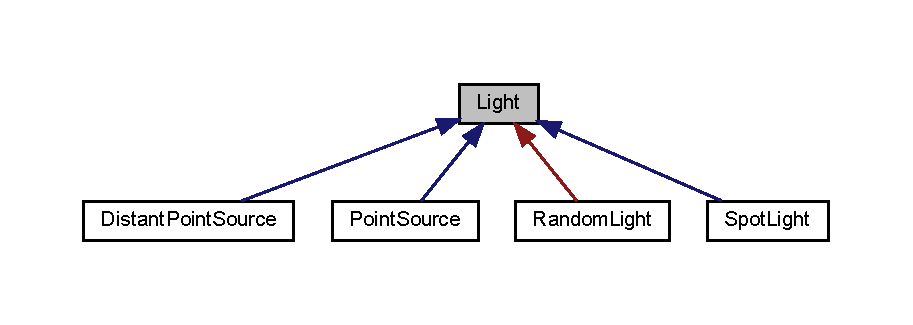
\includegraphics[width=350pt]{classLight__inherit__graph}
\end{center}
\end{figure}


Collaboration diagram for Light\+:
\nopagebreak
\begin{figure}[H]
\begin{center}
\leavevmode
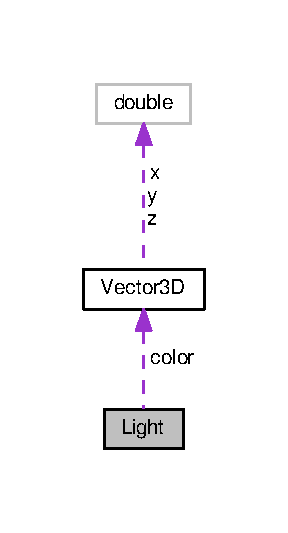
\includegraphics[width=138pt]{classLight__coll__graph}
\end{center}
\end{figure}
\subsection*{Public Member Functions}
\begin{DoxyCompactItemize}
\item 
virtual \mbox{\hyperlink{classRay}{Ray}} \mbox{\hyperlink{classLight_aa9c1529bb4a52128590e9b52d8a67517}{shaddow\+Ray}} (const \mbox{\hyperlink{classVector3D}{Vector3D}} \&pt) const
\begin{DoxyCompactList}\small\item\em This method is called to construct shaddow rays for this light-\/source. \end{DoxyCompactList}\item 
virtual \mbox{\hyperlink{classVector3D}{Vector3D}} \mbox{\hyperlink{classLight_a2a4cdf8081c2cab02757c2464610a32f}{specular\+Component}} (const \mbox{\hyperlink{classVector3D}{Vector3D}} \&pt) const =0
\item 
virtual \mbox{\hyperlink{classVector3D}{Vector3D}} \mbox{\hyperlink{classLight_af5dc859ada149ca54ec5088e1c33deb4}{diffuse\+Component}} (const \mbox{\hyperlink{classVector3D}{Vector3D}} \&pt) const =0
\item 
virtual \mbox{\hyperlink{classVector3D}{Vector3D}} \mbox{\hyperlink{classLight_ac075908cf22e9ca9f289c1226d133664}{get\+Light\+Direction}} (const \mbox{\hyperlink{classVector3D}{Vector3D}} \&pt) const =0
\item 
virtual double \mbox{\hyperlink{classLight_a4a7a5a9d4fc67da122c3ce75f6075093}{get\+Distance}} (\mbox{\hyperlink{classVector3D}{Vector3D}} point) const =0
\item 
virtual \mbox{\hyperlink{classLight_abe675054027c4b4a4f3e9a31d330931f}{$\sim$\+Light}} ()
\end{DoxyCompactItemize}
\subsection*{Private Attributes}
\begin{DoxyCompactItemize}
\item 
\mbox{\hyperlink{classVector3D}{Vector3D}} \mbox{\hyperlink{classLight_aea5f05e83e7f64b0a9360a52bcef2250}{color}}
\end{DoxyCompactItemize}


\subsection{Detailed Description}
Abstract class for lights used in \mbox{\hyperlink{classScene}{Scene}}. 

\subsection{Constructor \& Destructor Documentation}
\mbox{\Hypertarget{classLight_abe675054027c4b4a4f3e9a31d330931f}\label{classLight_abe675054027c4b4a4f3e9a31d330931f}} 
\index{Light@{Light}!````~Light@{$\sim$Light}}
\index{````~Light@{$\sim$Light}!Light@{Light}}
\subsubsection{\texorpdfstring{$\sim$Light()}{~Light()}}
{\footnotesize\ttfamily virtual Light\+::$\sim$\+Light (\begin{DoxyParamCaption}{ }\end{DoxyParamCaption})\hspace{0.3cm}{\ttfamily [inline]}, {\ttfamily [virtual]}}



\subsection{Member Function Documentation}
\mbox{\Hypertarget{classLight_af5dc859ada149ca54ec5088e1c33deb4}\label{classLight_af5dc859ada149ca54ec5088e1c33deb4}} 
\index{Light@{Light}!diffuseComponent@{diffuseComponent}}
\index{diffuseComponent@{diffuseComponent}!Light@{Light}}
\subsubsection{\texorpdfstring{diffuseComponent()}{diffuseComponent()}}
{\footnotesize\ttfamily virtual \mbox{\hyperlink{classVector3D}{Vector3D}} Light\+::diffuse\+Component (\begin{DoxyParamCaption}\item[{const \mbox{\hyperlink{classVector3D}{Vector3D}} \&}]{pt }\end{DoxyParamCaption}) const\hspace{0.3cm}{\ttfamily [pure virtual]}}



Implemented in \mbox{\hyperlink{classRandomLight_a371cbc5df30db46ac53cd0a9be91ac52}{Random\+Light}}, \mbox{\hyperlink{classPointSource_a445e9566d2226d1b8afd76274fb006fb}{Point\+Source}}, \mbox{\hyperlink{classDistantPointSource_ae3682ba2e553f38d6c9e4ee1bed9504f}{Distant\+Point\+Source}}, and \mbox{\hyperlink{classSpotLight_a0810e4bd136caddea0c65b819f2bd400}{Spot\+Light}}.

\mbox{\Hypertarget{classLight_a4a7a5a9d4fc67da122c3ce75f6075093}\label{classLight_a4a7a5a9d4fc67da122c3ce75f6075093}} 
\index{Light@{Light}!getDistance@{getDistance}}
\index{getDistance@{getDistance}!Light@{Light}}
\subsubsection{\texorpdfstring{getDistance()}{getDistance()}}
{\footnotesize\ttfamily virtual double Light\+::get\+Distance (\begin{DoxyParamCaption}\item[{\mbox{\hyperlink{classVector3D}{Vector3D}}}]{point }\end{DoxyParamCaption}) const\hspace{0.3cm}{\ttfamily [pure virtual]}}



Implemented in \mbox{\hyperlink{classPointSource_a5f1af9abccf0657b9398555c935bb8bc}{Point\+Source}}, \mbox{\hyperlink{classDistantPointSource_a5d08b5655fc7fc09e5c0d2a0f3046e16}{Distant\+Point\+Source}}, and \mbox{\hyperlink{classSpotLight_a117f7918773e193f67714765c5370418}{Spot\+Light}}.

\mbox{\Hypertarget{classLight_ac075908cf22e9ca9f289c1226d133664}\label{classLight_ac075908cf22e9ca9f289c1226d133664}} 
\index{Light@{Light}!getLightDirection@{getLightDirection}}
\index{getLightDirection@{getLightDirection}!Light@{Light}}
\subsubsection{\texorpdfstring{getLightDirection()}{getLightDirection()}}
{\footnotesize\ttfamily virtual \mbox{\hyperlink{classVector3D}{Vector3D}} Light\+::get\+Light\+Direction (\begin{DoxyParamCaption}\item[{const \mbox{\hyperlink{classVector3D}{Vector3D}} \&}]{pt }\end{DoxyParamCaption}) const\hspace{0.3cm}{\ttfamily [pure virtual]}}



Implemented in \mbox{\hyperlink{classPointSource_a02a13a7b955088e32324bfb3d49b1ace}{Point\+Source}}, \mbox{\hyperlink{classDistantPointSource_a740ee32c41e2ef6deec1137c86f5b73a}{Distant\+Point\+Source}}, \mbox{\hyperlink{classSpotLight_a051e210b637edf37bf2b8d49149a13a4}{Spot\+Light}}, and \mbox{\hyperlink{classRandomLight_a70c038d63e66f520a296dccddcf9035f}{Random\+Light}}.

\mbox{\Hypertarget{classLight_aa9c1529bb4a52128590e9b52d8a67517}\label{classLight_aa9c1529bb4a52128590e9b52d8a67517}} 
\index{Light@{Light}!shaddowRay@{shaddowRay}}
\index{shaddowRay@{shaddowRay}!Light@{Light}}
\subsubsection{\texorpdfstring{shaddowRay()}{shaddowRay()}}
{\footnotesize\ttfamily \mbox{\hyperlink{classRay}{Ray}} Light\+::shaddow\+Ray (\begin{DoxyParamCaption}\item[{const \mbox{\hyperlink{classVector3D}{Vector3D}} \&}]{pt }\end{DoxyParamCaption}) const\hspace{0.3cm}{\ttfamily [virtual]}}



This method is called to construct shaddow rays for this light-\/source. 


\begin{DoxyParams}{Parameters}
{\em pt} & A point in 3D-\/\+Space at which the shaddow-\/ray originates \\
\hline
\end{DoxyParams}
\begin{DoxyReturn}{Returns}
A ray originating in pt, pointing at this light 
\end{DoxyReturn}
\mbox{\Hypertarget{classLight_a2a4cdf8081c2cab02757c2464610a32f}\label{classLight_a2a4cdf8081c2cab02757c2464610a32f}} 
\index{Light@{Light}!specularComponent@{specularComponent}}
\index{specularComponent@{specularComponent}!Light@{Light}}
\subsubsection{\texorpdfstring{specularComponent()}{specularComponent()}}
{\footnotesize\ttfamily virtual \mbox{\hyperlink{classVector3D}{Vector3D}} Light\+::specular\+Component (\begin{DoxyParamCaption}\item[{const \mbox{\hyperlink{classVector3D}{Vector3D}} \&}]{pt }\end{DoxyParamCaption}) const\hspace{0.3cm}{\ttfamily [pure virtual]}}



Implemented in \mbox{\hyperlink{classPointSource_a421e0e8d3d1f69aeb095f1f9c39de7e0}{Point\+Source}}, \mbox{\hyperlink{classDistantPointSource_a14f9c55d090d7d3f7999db70f5174a8c}{Distant\+Point\+Source}}, \mbox{\hyperlink{classRandomLight_af9922ba2ce0c9dc16026db945d8f1506}{Random\+Light}}, and \mbox{\hyperlink{classSpotLight_a6a1cc6970bbb3308b5214f85641331cd}{Spot\+Light}}.



\subsection{Member Data Documentation}
\mbox{\Hypertarget{classLight_aea5f05e83e7f64b0a9360a52bcef2250}\label{classLight_aea5f05e83e7f64b0a9360a52bcef2250}} 
\index{Light@{Light}!color@{color}}
\index{color@{color}!Light@{Light}}
\subsubsection{\texorpdfstring{color}{color}}
{\footnotesize\ttfamily \mbox{\hyperlink{classVector3D}{Vector3D}} Light\+::color\hspace{0.3cm}{\ttfamily [private]}}



The documentation for this class was generated from the following files\+:\begin{DoxyCompactItemize}
\item 
src/\mbox{\hyperlink{Light_8h}{Light.\+h}}\item 
src/\mbox{\hyperlink{Light_8cpp}{Light.\+cpp}}\end{DoxyCompactItemize}

\hypertarget{unionBVHLinearNode_1_1LinearSecondChild}{}\section{B\+V\+H\+Linear\+Node\+::Linear\+Second\+Child Union Reference}
\label{unionBVHLinearNode_1_1LinearSecondChild}\index{BVHLinearNode::LinearSecondChild@{BVHLinearNode::LinearSecondChild}}


{\ttfamily \#include $<$Binary\+Volume\+Hierarchy.\+h$>$}



Collaboration diagram for B\+V\+H\+Linear\+Node\+::Linear\+Second\+Child\+:
\nopagebreak
\begin{figure}[H]
\begin{center}
\leavevmode
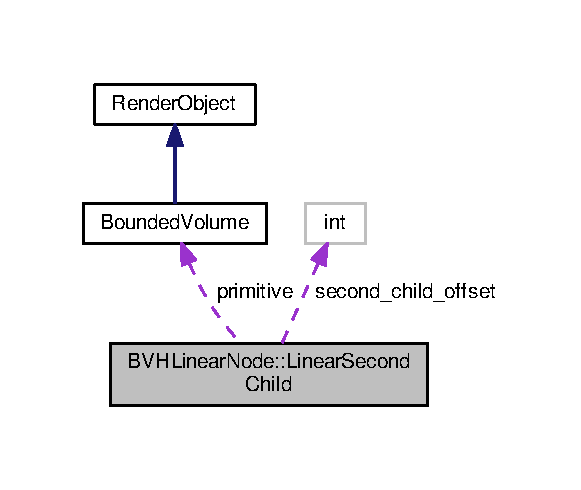
\includegraphics[width=275pt]{unionBVHLinearNode_1_1LinearSecondChild__coll__graph}
\end{center}
\end{figure}
\subsection*{Public Attributes}
\begin{DoxyCompactItemize}
\item 
\mbox{\hyperlink{classBoundedVolume}{Bounded\+Volume}} $\ast$ \mbox{\hyperlink{unionBVHLinearNode_1_1LinearSecondChild_ac8489c14e68bc1f8fee2cdf842199e61}{primitive}}
\item 
unsigned int \mbox{\hyperlink{unionBVHLinearNode_1_1LinearSecondChild_ac0a41d4aa3236a1f51741467112ee9ba}{second\+\_\+child\+\_\+offset}}
\end{DoxyCompactItemize}


\subsection{Member Data Documentation}
\mbox{\Hypertarget{unionBVHLinearNode_1_1LinearSecondChild_ac8489c14e68bc1f8fee2cdf842199e61}\label{unionBVHLinearNode_1_1LinearSecondChild_ac8489c14e68bc1f8fee2cdf842199e61}} 
\index{BVHLinearNode::LinearSecondChild@{BVHLinearNode::LinearSecondChild}!primitive@{primitive}}
\index{primitive@{primitive}!BVHLinearNode::LinearSecondChild@{BVHLinearNode::LinearSecondChild}}
\subsubsection{\texorpdfstring{primitive}{primitive}}
{\footnotesize\ttfamily \mbox{\hyperlink{classBoundedVolume}{Bounded\+Volume}}$\ast$ B\+V\+H\+Linear\+Node\+::\+Linear\+Second\+Child\+::primitive}

\mbox{\Hypertarget{unionBVHLinearNode_1_1LinearSecondChild_ac0a41d4aa3236a1f51741467112ee9ba}\label{unionBVHLinearNode_1_1LinearSecondChild_ac0a41d4aa3236a1f51741467112ee9ba}} 
\index{BVHLinearNode::LinearSecondChild@{BVHLinearNode::LinearSecondChild}!second\_child\_offset@{second\_child\_offset}}
\index{second\_child\_offset@{second\_child\_offset}!BVHLinearNode::LinearSecondChild@{BVHLinearNode::LinearSecondChild}}
\subsubsection{\texorpdfstring{second\_child\_offset}{second\_child\_offset}}
{\footnotesize\ttfamily unsigned int B\+V\+H\+Linear\+Node\+::\+Linear\+Second\+Child\+::second\+\_\+child\+\_\+offset}



The documentation for this union was generated from the following file\+:\begin{DoxyCompactItemize}
\item 
src/renderable/\mbox{\hyperlink{BinaryVolumeHierarchy_8h}{Binary\+Volume\+Hierarchy.\+h}}\end{DoxyCompactItemize}

\hypertarget{classsymcpp_1_1Logarithm}{}\section{symcpp\+::Logarithm Class Reference}
\label{classsymcpp_1_1Logarithm}\index{symcpp::Logarithm@{symcpp::Logarithm}}


{\ttfamily \#include $<$Logarithm.\+h$>$}



Inheritance diagram for symcpp\+::Logarithm\+:
\nopagebreak
\begin{figure}[H]
\begin{center}
\leavevmode
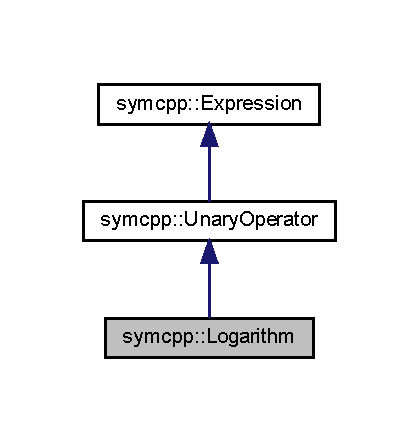
\includegraphics[width=201pt]{classsymcpp_1_1Logarithm__inherit__graph}
\end{center}
\end{figure}


Collaboration diagram for symcpp\+::Logarithm\+:
\nopagebreak
\begin{figure}[H]
\begin{center}
\leavevmode
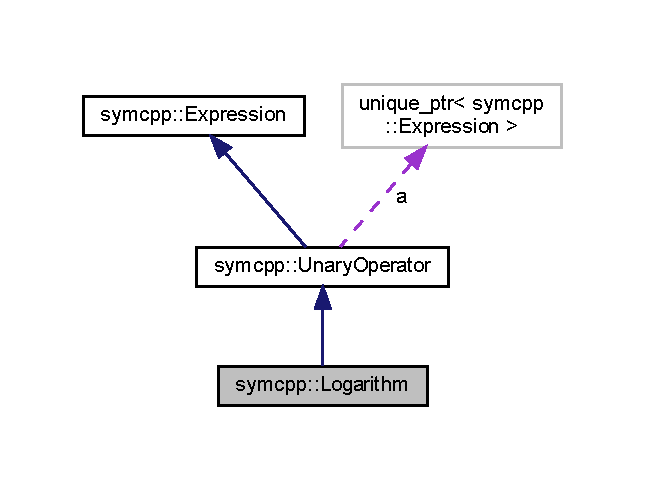
\includegraphics[width=310pt]{classsymcpp_1_1Logarithm__coll__graph}
\end{center}
\end{figure}
\subsection*{Public Member Functions}
\begin{DoxyCompactItemize}
\item 
std\+::unique\+\_\+ptr$<$ \mbox{\hyperlink{classsymcpp_1_1Expression}{Expression}} $>$ \mbox{\hyperlink{classsymcpp_1_1Logarithm_ac7315464088f7ef34cfce74e518b939a}{copy}} () const override
\item 
std\+::unique\+\_\+ptr$<$ \mbox{\hyperlink{classsymcpp_1_1Expression}{Expression}} $>$ \mbox{\hyperlink{classsymcpp_1_1Logarithm_af771894e90cbe561e3eb2e9a9b32954b}{simplify}} () override
\item 
\mbox{\hyperlink{classsymcpp_1_1Logarithm_a23a8172db96675ebf1114f4f3f41b6f1}{Unary\+Operator}} (const \mbox{\hyperlink{classsymcpp_1_1Expression}{Expression}} \&\mbox{\hyperlink{classsymcpp_1_1UnaryOperator_a1558842963261562d2ef68e324822cba}{a}})
\item 
\mbox{\hyperlink{classsymcpp_1_1Logarithm_ad3aa899567a080eeb41cb850de310178}{Unary\+Operator}} (std\+::unique\+\_\+ptr$<$ \mbox{\hyperlink{classsymcpp_1_1Expression}{Expression}} $>$ \&\&\mbox{\hyperlink{classsymcpp_1_1UnaryOperator_a1558842963261562d2ef68e324822cba}{a}})
\end{DoxyCompactItemize}
\subsection*{Private Member Functions}
\begin{DoxyCompactItemize}
\item 
double \mbox{\hyperlink{classsymcpp_1_1Logarithm_a349cbd26700ea28d18a42f6f8d7e722c}{op}} (double x) const override
\item 
std\+::ostream \& \mbox{\hyperlink{classsymcpp_1_1Logarithm_a336bed1a474b338eabd6a258d527b65b}{print}} (std\+::ostream \&sink) const override
\item 
std\+::unique\+\_\+ptr$<$ \mbox{\hyperlink{classsymcpp_1_1Expression}{Expression}} $>$ \mbox{\hyperlink{classsymcpp_1_1Logarithm_ab5cb1daed6613731d15ee13d17c48f7b}{partial\+\_\+derivative}} () const override
\end{DoxyCompactItemize}
\subsection*{Additional Inherited Members}


\subsection{Member Function Documentation}
\mbox{\Hypertarget{classsymcpp_1_1Logarithm_ac7315464088f7ef34cfce74e518b939a}\label{classsymcpp_1_1Logarithm_ac7315464088f7ef34cfce74e518b939a}} 
\index{symcpp::Logarithm@{symcpp::Logarithm}!copy@{copy}}
\index{copy@{copy}!symcpp::Logarithm@{symcpp::Logarithm}}
\subsubsection{\texorpdfstring{copy()}{copy()}}
{\footnotesize\ttfamily std\+::unique\+\_\+ptr$<$ \mbox{\hyperlink{classsymcpp_1_1Expression}{Expression}} $>$ symcpp\+::\+Logarithm\+::copy (\begin{DoxyParamCaption}{ }\end{DoxyParamCaption}) const\hspace{0.3cm}{\ttfamily [override]}, {\ttfamily [virtual]}}



Implements \mbox{\hyperlink{classsymcpp_1_1Expression_a2e7de5a295ccf0efdc9b34cea7ba3d0b}{symcpp\+::\+Expression}}.

\mbox{\Hypertarget{classsymcpp_1_1Logarithm_a349cbd26700ea28d18a42f6f8d7e722c}\label{classsymcpp_1_1Logarithm_a349cbd26700ea28d18a42f6f8d7e722c}} 
\index{symcpp::Logarithm@{symcpp::Logarithm}!op@{op}}
\index{op@{op}!symcpp::Logarithm@{symcpp::Logarithm}}
\subsubsection{\texorpdfstring{op()}{op()}}
{\footnotesize\ttfamily double symcpp\+::\+Logarithm\+::op (\begin{DoxyParamCaption}\item[{double}]{x }\end{DoxyParamCaption}) const\hspace{0.3cm}{\ttfamily [override]}, {\ttfamily [private]}, {\ttfamily [virtual]}}



Implements \mbox{\hyperlink{classsymcpp_1_1UnaryOperator_a679c3c46cad3a62bdd776ff836c7891e}{symcpp\+::\+Unary\+Operator}}.

\mbox{\Hypertarget{classsymcpp_1_1Logarithm_ab5cb1daed6613731d15ee13d17c48f7b}\label{classsymcpp_1_1Logarithm_ab5cb1daed6613731d15ee13d17c48f7b}} 
\index{symcpp::Logarithm@{symcpp::Logarithm}!partial\_derivative@{partial\_derivative}}
\index{partial\_derivative@{partial\_derivative}!symcpp::Logarithm@{symcpp::Logarithm}}
\subsubsection{\texorpdfstring{partial\_derivative()}{partial\_derivative()}}
{\footnotesize\ttfamily std\+::unique\+\_\+ptr$<$ \mbox{\hyperlink{classsymcpp_1_1Expression}{Expression}} $>$ symcpp\+::\+Logarithm\+::partial\+\_\+derivative (\begin{DoxyParamCaption}{ }\end{DoxyParamCaption}) const\hspace{0.3cm}{\ttfamily [override]}, {\ttfamily [private]}, {\ttfamily [virtual]}}



Implements \mbox{\hyperlink{classsymcpp_1_1UnaryOperator_a85de3214870cd72edc63ac1c221ddeee}{symcpp\+::\+Unary\+Operator}}.

\mbox{\Hypertarget{classsymcpp_1_1Logarithm_a336bed1a474b338eabd6a258d527b65b}\label{classsymcpp_1_1Logarithm_a336bed1a474b338eabd6a258d527b65b}} 
\index{symcpp::Logarithm@{symcpp::Logarithm}!print@{print}}
\index{print@{print}!symcpp::Logarithm@{symcpp::Logarithm}}
\subsubsection{\texorpdfstring{print()}{print()}}
{\footnotesize\ttfamily std\+::ostream \& symcpp\+::\+Logarithm\+::print (\begin{DoxyParamCaption}\item[{std\+::ostream \&}]{sink }\end{DoxyParamCaption}) const\hspace{0.3cm}{\ttfamily [override]}, {\ttfamily [private]}, {\ttfamily [virtual]}}



Implements \mbox{\hyperlink{classsymcpp_1_1Expression_af37e13032a40f2da4d2866eaa8658049}{symcpp\+::\+Expression}}.

\mbox{\Hypertarget{classsymcpp_1_1Logarithm_af771894e90cbe561e3eb2e9a9b32954b}\label{classsymcpp_1_1Logarithm_af771894e90cbe561e3eb2e9a9b32954b}} 
\index{symcpp::Logarithm@{symcpp::Logarithm}!simplify@{simplify}}
\index{simplify@{simplify}!symcpp::Logarithm@{symcpp::Logarithm}}
\subsubsection{\texorpdfstring{simplify()}{simplify()}}
{\footnotesize\ttfamily std\+::unique\+\_\+ptr$<$ \mbox{\hyperlink{classsymcpp_1_1Expression}{Expression}} $>$ symcpp\+::\+Logarithm\+::simplify (\begin{DoxyParamCaption}{ }\end{DoxyParamCaption})\hspace{0.3cm}{\ttfamily [override]}, {\ttfamily [virtual]}}



Implements \mbox{\hyperlink{classsymcpp_1_1Expression_ab1fa6e55eea0682250d013f28db26cd2}{symcpp\+::\+Expression}}.

\mbox{\Hypertarget{classsymcpp_1_1Logarithm_ad3aa899567a080eeb41cb850de310178}\label{classsymcpp_1_1Logarithm_ad3aa899567a080eeb41cb850de310178}} 
\index{symcpp::Logarithm@{symcpp::Logarithm}!UnaryOperator@{UnaryOperator}}
\index{UnaryOperator@{UnaryOperator}!symcpp::Logarithm@{symcpp::Logarithm}}
\subsubsection{\texorpdfstring{UnaryOperator()}{UnaryOperator()}\hspace{0.1cm}{\footnotesize\ttfamily [1/2]}}
{\footnotesize\ttfamily symcpp\+::\+Unary\+Operator\+::\+Unary\+Operator\hspace{0.3cm}{\ttfamily [inline]}}

\mbox{\Hypertarget{classsymcpp_1_1Logarithm_a23a8172db96675ebf1114f4f3f41b6f1}\label{classsymcpp_1_1Logarithm_a23a8172db96675ebf1114f4f3f41b6f1}} 
\index{symcpp::Logarithm@{symcpp::Logarithm}!UnaryOperator@{UnaryOperator}}
\index{UnaryOperator@{UnaryOperator}!symcpp::Logarithm@{symcpp::Logarithm}}
\subsubsection{\texorpdfstring{UnaryOperator()}{UnaryOperator()}\hspace{0.1cm}{\footnotesize\ttfamily [2/2]}}
{\footnotesize\ttfamily symcpp\+::\+Unary\+Operator\+::\+Unary\+Operator\hspace{0.3cm}{\ttfamily [inline]}}



The documentation for this class was generated from the following files\+:\begin{DoxyCompactItemize}
\item 
src/symcpp/\mbox{\hyperlink{Logarithm_8h}{Logarithm.\+h}}\item 
src/symcpp/\mbox{\hyperlink{Logarithm_8cpp}{Logarithm.\+cpp}}\end{DoxyCompactItemize}

\hypertarget{classMaterial}{}\section{Material Class Reference}
\label{classMaterial}\index{Material@{Material}}


Typically stores information about material of Render\+Objects.  




{\ttfamily \#include $<$Material.\+h$>$}



Collaboration diagram for Material\+:\nopagebreak
\begin{figure}[H]
\begin{center}
\leavevmode
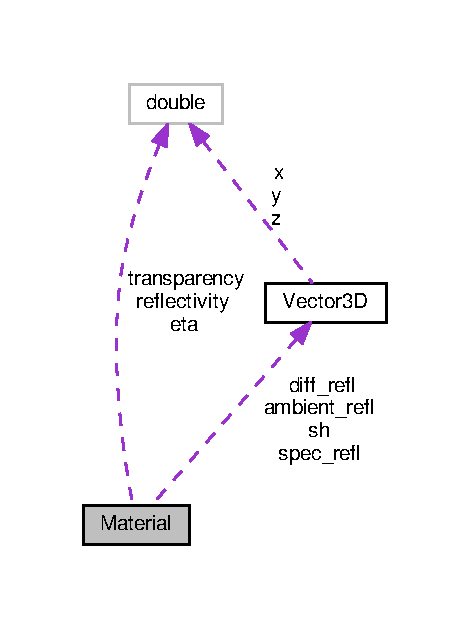
\includegraphics[width=226pt]{classMaterial__coll__graph}
\end{center}
\end{figure}
\subsection*{Public Member Functions}
\begin{DoxyCompactItemize}
\item 
\hyperlink{classMaterial_a4e63e7e70f9a2cc55801f798d88f5c14}{Material} (const \hyperlink{classVector3D}{Vector3D} \&\hyperlink{classMaterial_a8b1858703e3298ba1cc705684939f953}{spec\+\_\+refl}, const \hyperlink{classVector3D}{Vector3D} \&\hyperlink{classMaterial_af53038fbe5bbe5d1a9801aabc97543a5}{diff\+\_\+refl}, const \hyperlink{classVector3D}{Vector3D} \&\hyperlink{classMaterial_a40002cba7c7049feb2bddaf57ae96ba4}{ambient\+\_\+refl}, const \hyperlink{classVector3D}{Vector3D} \&\hyperlink{classMaterial_abd4573ad64b9e4ebc7d3a365e2078d69}{shininess}, double \hyperlink{classMaterial_a02abe03436775e128e04e1c737d34067}{transparency}, double \hyperlink{classMaterial_a050f60e6002271e571c4e5afc4b097b5}{reflectivity}, double \hyperlink{classMaterial_a62e8368c76c975790315b16d97558c26}{eta})
\item 
\hyperlink{classMaterial_a6059ec72855855b11672ff25962e9336}{Material} ()=default
\item 
\hyperlink{classVector3D}{Vector3D} \& \hyperlink{classMaterial_a927c720ad76f97c4619dca4a1b609b26}{specular\+\_\+reflectivity} ()
\item 
\hyperlink{classVector3D}{Vector3D} \& \hyperlink{classMaterial_a3f4ff9c259e67dcffa2d607f788fd2a1}{diffuse\+\_\+reflectivity} ()
\item 
\hyperlink{classVector3D}{Vector3D} \& \hyperlink{classMaterial_a2b80ada55bf639ce99daa45f8c94bfc6}{ambient\+\_\+reflectivity} ()
\item 
\hyperlink{classVector3D}{Vector3D} \& \hyperlink{classMaterial_abd4573ad64b9e4ebc7d3a365e2078d69}{shininess} ()
\item 
bool \hyperlink{classMaterial_abec78805fbfef252c880c2208c5c26be}{is\+\_\+reflective} () const 
\item 
double \hyperlink{classMaterial_a29eeea5a383619c64e2014ea44962911}{get\+\_\+reflectivity} () const 
\item 
double \hyperlink{classMaterial_a55764b81a00d8908593c9cf7caec655a}{get\+\_\+transparency} () const 
\item 
bool \hyperlink{classMaterial_acf9c74cabb160d0e8e6445ae3f39d3b9}{is\+\_\+transparent} () const 
\item 
double \hyperlink{classMaterial_a1f580e086d0775df267fa4c791713834}{get\+\_\+index} () const 
\item 
std\+::ostream \& \hyperlink{classMaterial_a9b45a3e49fbc8e4eb7ba30839ed6d593}{print} (std\+::ostream \&sink) const 
\end{DoxyCompactItemize}
\subsection*{Private Attributes}
\begin{DoxyCompactItemize}
\item 
\hyperlink{classVector3D}{Vector3D} \hyperlink{classMaterial_a8b1858703e3298ba1cc705684939f953}{spec\+\_\+refl}
\item 
\hyperlink{classVector3D}{Vector3D} \hyperlink{classMaterial_af53038fbe5bbe5d1a9801aabc97543a5}{diff\+\_\+refl}
\item 
\hyperlink{classVector3D}{Vector3D} \hyperlink{classMaterial_a40002cba7c7049feb2bddaf57ae96ba4}{ambient\+\_\+refl}
\item 
\hyperlink{classVector3D}{Vector3D} \hyperlink{classMaterial_a886d30c3aaf819eea8f619c5ecc21f92}{sh}
\item 
double \hyperlink{classMaterial_a02abe03436775e128e04e1c737d34067}{transparency}
\item 
double \hyperlink{classMaterial_a050f60e6002271e571c4e5afc4b097b5}{reflectivity}
\item 
double \hyperlink{classMaterial_a62e8368c76c975790315b16d97558c26}{eta}
\end{DoxyCompactItemize}
\subsection*{Friends}
\begin{DoxyCompactItemize}
\item 
class \hyperlink{classMaterial_aa4d43ed50061aeb4600daf1e3f7706ac}{M\+T\+L\+Lib}
\item 
std\+::ostream \& \hyperlink{classMaterial_acf2af134f767709233736d54356180be}{operator$<$$<$} (std\+::ostream \&sink, const \hyperlink{classMaterial}{Material} \&mat)
\end{DoxyCompactItemize}


\subsection{Detailed Description}
Typically stores information about material of Render\+Objects. 

\subsection{Constructor \& Destructor Documentation}
\index{Material@{Material}!Material@{Material}}
\index{Material@{Material}!Material@{Material}}
\subsubsection[{\texorpdfstring{Material(const Vector3\+D \&spec\+\_\+refl, const Vector3\+D \&diff\+\_\+refl, const Vector3\+D \&ambient\+\_\+refl, const Vector3\+D \&shininess, double transparency, double reflectivity, double eta)}{Material(const Vector3D &spec_refl, const Vector3D &diff_refl, const Vector3D &ambient_refl, const Vector3D &shininess, double transparency, double reflectivity, double eta)}}]{\setlength{\rightskip}{0pt plus 5cm}Material\+::\+Material (
\begin{DoxyParamCaption}
\item[{const {\bf Vector3D} \&}]{spec\+\_\+refl, }
\item[{const {\bf Vector3D} \&}]{diff\+\_\+refl, }
\item[{const {\bf Vector3D} \&}]{ambient\+\_\+refl, }
\item[{const {\bf Vector3D} \&}]{shininess, }
\item[{double}]{transparency, }
\item[{double}]{reflectivity, }
\item[{double}]{eta}
\end{DoxyParamCaption}
)}\hypertarget{classMaterial_a4e63e7e70f9a2cc55801f798d88f5c14}{}\label{classMaterial_a4e63e7e70f9a2cc55801f798d88f5c14}
\index{Material@{Material}!Material@{Material}}
\index{Material@{Material}!Material@{Material}}
\subsubsection[{\texorpdfstring{Material()=default}{Material()=default}}]{\setlength{\rightskip}{0pt plus 5cm}Material\+::\+Material (
\begin{DoxyParamCaption}
{}
\end{DoxyParamCaption}
)\hspace{0.3cm}{\ttfamily [default]}}\hypertarget{classMaterial_a6059ec72855855b11672ff25962e9336}{}\label{classMaterial_a6059ec72855855b11672ff25962e9336}


\subsection{Member Function Documentation}
\index{Material@{Material}!ambient\+\_\+reflectivity@{ambient\+\_\+reflectivity}}
\index{ambient\+\_\+reflectivity@{ambient\+\_\+reflectivity}!Material@{Material}}
\subsubsection[{\texorpdfstring{ambient\+\_\+reflectivity()}{ambient_reflectivity()}}]{\setlength{\rightskip}{0pt plus 5cm}{\bf Vector3D} \& Material\+::ambient\+\_\+reflectivity (
\begin{DoxyParamCaption}
{}
\end{DoxyParamCaption}
)}\hypertarget{classMaterial_a2b80ada55bf639ce99daa45f8c94bfc6}{}\label{classMaterial_a2b80ada55bf639ce99daa45f8c94bfc6}
\index{Material@{Material}!diffuse\+\_\+reflectivity@{diffuse\+\_\+reflectivity}}
\index{diffuse\+\_\+reflectivity@{diffuse\+\_\+reflectivity}!Material@{Material}}
\subsubsection[{\texorpdfstring{diffuse\+\_\+reflectivity()}{diffuse_reflectivity()}}]{\setlength{\rightskip}{0pt plus 5cm}{\bf Vector3D} \& Material\+::diffuse\+\_\+reflectivity (
\begin{DoxyParamCaption}
{}
\end{DoxyParamCaption}
)}\hypertarget{classMaterial_a3f4ff9c259e67dcffa2d607f788fd2a1}{}\label{classMaterial_a3f4ff9c259e67dcffa2d607f788fd2a1}
\index{Material@{Material}!get\+\_\+index@{get\+\_\+index}}
\index{get\+\_\+index@{get\+\_\+index}!Material@{Material}}
\subsubsection[{\texorpdfstring{get\+\_\+index() const }{get_index() const }}]{\setlength{\rightskip}{0pt plus 5cm}double Material\+::get\+\_\+index (
\begin{DoxyParamCaption}
{}
\end{DoxyParamCaption}
) const}\hypertarget{classMaterial_a1f580e086d0775df267fa4c791713834}{}\label{classMaterial_a1f580e086d0775df267fa4c791713834}
\index{Material@{Material}!get\+\_\+reflectivity@{get\+\_\+reflectivity}}
\index{get\+\_\+reflectivity@{get\+\_\+reflectivity}!Material@{Material}}
\subsubsection[{\texorpdfstring{get\+\_\+reflectivity() const }{get_reflectivity() const }}]{\setlength{\rightskip}{0pt plus 5cm}double Material\+::get\+\_\+reflectivity (
\begin{DoxyParamCaption}
{}
\end{DoxyParamCaption}
) const}\hypertarget{classMaterial_a29eeea5a383619c64e2014ea44962911}{}\label{classMaterial_a29eeea5a383619c64e2014ea44962911}
\index{Material@{Material}!get\+\_\+transparency@{get\+\_\+transparency}}
\index{get\+\_\+transparency@{get\+\_\+transparency}!Material@{Material}}
\subsubsection[{\texorpdfstring{get\+\_\+transparency() const }{get_transparency() const }}]{\setlength{\rightskip}{0pt plus 5cm}double Material\+::get\+\_\+transparency (
\begin{DoxyParamCaption}
{}
\end{DoxyParamCaption}
) const}\hypertarget{classMaterial_a55764b81a00d8908593c9cf7caec655a}{}\label{classMaterial_a55764b81a00d8908593c9cf7caec655a}
\index{Material@{Material}!is\+\_\+reflective@{is\+\_\+reflective}}
\index{is\+\_\+reflective@{is\+\_\+reflective}!Material@{Material}}
\subsubsection[{\texorpdfstring{is\+\_\+reflective() const }{is_reflective() const }}]{\setlength{\rightskip}{0pt plus 5cm}bool Material\+::is\+\_\+reflective (
\begin{DoxyParamCaption}
{}
\end{DoxyParamCaption}
) const}\hypertarget{classMaterial_abec78805fbfef252c880c2208c5c26be}{}\label{classMaterial_abec78805fbfef252c880c2208c5c26be}
\index{Material@{Material}!is\+\_\+transparent@{is\+\_\+transparent}}
\index{is\+\_\+transparent@{is\+\_\+transparent}!Material@{Material}}
\subsubsection[{\texorpdfstring{is\+\_\+transparent() const }{is_transparent() const }}]{\setlength{\rightskip}{0pt plus 5cm}bool Material\+::is\+\_\+transparent (
\begin{DoxyParamCaption}
{}
\end{DoxyParamCaption}
) const}\hypertarget{classMaterial_acf9c74cabb160d0e8e6445ae3f39d3b9}{}\label{classMaterial_acf9c74cabb160d0e8e6445ae3f39d3b9}
\index{Material@{Material}!print@{print}}
\index{print@{print}!Material@{Material}}
\subsubsection[{\texorpdfstring{print(std\+::ostream \&sink) const }{print(std::ostream &sink) const }}]{\setlength{\rightskip}{0pt plus 5cm}std\+::ostream \& Material\+::print (
\begin{DoxyParamCaption}
\item[{std\+::ostream \&}]{sink}
\end{DoxyParamCaption}
) const}\hypertarget{classMaterial_a9b45a3e49fbc8e4eb7ba30839ed6d593}{}\label{classMaterial_a9b45a3e49fbc8e4eb7ba30839ed6d593}
\index{Material@{Material}!shininess@{shininess}}
\index{shininess@{shininess}!Material@{Material}}
\subsubsection[{\texorpdfstring{shininess()}{shininess()}}]{\setlength{\rightskip}{0pt plus 5cm}{\bf Vector3D} \& Material\+::shininess (
\begin{DoxyParamCaption}
{}
\end{DoxyParamCaption}
)}\hypertarget{classMaterial_abd4573ad64b9e4ebc7d3a365e2078d69}{}\label{classMaterial_abd4573ad64b9e4ebc7d3a365e2078d69}
\index{Material@{Material}!specular\+\_\+reflectivity@{specular\+\_\+reflectivity}}
\index{specular\+\_\+reflectivity@{specular\+\_\+reflectivity}!Material@{Material}}
\subsubsection[{\texorpdfstring{specular\+\_\+reflectivity()}{specular_reflectivity()}}]{\setlength{\rightskip}{0pt plus 5cm}{\bf Vector3D} \& Material\+::specular\+\_\+reflectivity (
\begin{DoxyParamCaption}
{}
\end{DoxyParamCaption}
)}\hypertarget{classMaterial_a927c720ad76f97c4619dca4a1b609b26}{}\label{classMaterial_a927c720ad76f97c4619dca4a1b609b26}


\subsection{Friends And Related Function Documentation}
\index{Material@{Material}!M\+T\+L\+Lib@{M\+T\+L\+Lib}}
\index{M\+T\+L\+Lib@{M\+T\+L\+Lib}!Material@{Material}}
\subsubsection[{\texorpdfstring{M\+T\+L\+Lib}{MTLLib}}]{\setlength{\rightskip}{0pt plus 5cm}friend class {\bf M\+T\+L\+Lib}\hspace{0.3cm}{\ttfamily [friend]}}\hypertarget{classMaterial_aa4d43ed50061aeb4600daf1e3f7706ac}{}\label{classMaterial_aa4d43ed50061aeb4600daf1e3f7706ac}
\index{Material@{Material}!operator$<$$<$@{operator$<$$<$}}
\index{operator$<$$<$@{operator$<$$<$}!Material@{Material}}
\subsubsection[{\texorpdfstring{operator$<$$<$}{operator<<}}]{\setlength{\rightskip}{0pt plus 5cm}std\+::ostream\& operator$<$$<$ (
\begin{DoxyParamCaption}
\item[{std\+::ostream \&}]{sink, }
\item[{const {\bf Material} \&}]{mat}
\end{DoxyParamCaption}
)\hspace{0.3cm}{\ttfamily [friend]}}\hypertarget{classMaterial_acf2af134f767709233736d54356180be}{}\label{classMaterial_acf2af134f767709233736d54356180be}


\subsection{Member Data Documentation}
\index{Material@{Material}!ambient\+\_\+refl@{ambient\+\_\+refl}}
\index{ambient\+\_\+refl@{ambient\+\_\+refl}!Material@{Material}}
\subsubsection[{\texorpdfstring{ambient\+\_\+refl}{ambient_refl}}]{\setlength{\rightskip}{0pt plus 5cm}{\bf Vector3D} Material\+::ambient\+\_\+refl\hspace{0.3cm}{\ttfamily [private]}}\hypertarget{classMaterial_a40002cba7c7049feb2bddaf57ae96ba4}{}\label{classMaterial_a40002cba7c7049feb2bddaf57ae96ba4}
\index{Material@{Material}!diff\+\_\+refl@{diff\+\_\+refl}}
\index{diff\+\_\+refl@{diff\+\_\+refl}!Material@{Material}}
\subsubsection[{\texorpdfstring{diff\+\_\+refl}{diff_refl}}]{\setlength{\rightskip}{0pt plus 5cm}{\bf Vector3D} Material\+::diff\+\_\+refl\hspace{0.3cm}{\ttfamily [private]}}\hypertarget{classMaterial_af53038fbe5bbe5d1a9801aabc97543a5}{}\label{classMaterial_af53038fbe5bbe5d1a9801aabc97543a5}
\index{Material@{Material}!eta@{eta}}
\index{eta@{eta}!Material@{Material}}
\subsubsection[{\texorpdfstring{eta}{eta}}]{\setlength{\rightskip}{0pt plus 5cm}double Material\+::eta\hspace{0.3cm}{\ttfamily [private]}}\hypertarget{classMaterial_a62e8368c76c975790315b16d97558c26}{}\label{classMaterial_a62e8368c76c975790315b16d97558c26}
\index{Material@{Material}!reflectivity@{reflectivity}}
\index{reflectivity@{reflectivity}!Material@{Material}}
\subsubsection[{\texorpdfstring{reflectivity}{reflectivity}}]{\setlength{\rightskip}{0pt plus 5cm}double Material\+::reflectivity\hspace{0.3cm}{\ttfamily [private]}}\hypertarget{classMaterial_a050f60e6002271e571c4e5afc4b097b5}{}\label{classMaterial_a050f60e6002271e571c4e5afc4b097b5}
\index{Material@{Material}!sh@{sh}}
\index{sh@{sh}!Material@{Material}}
\subsubsection[{\texorpdfstring{sh}{sh}}]{\setlength{\rightskip}{0pt plus 5cm}{\bf Vector3D} Material\+::sh\hspace{0.3cm}{\ttfamily [private]}}\hypertarget{classMaterial_a886d30c3aaf819eea8f619c5ecc21f92}{}\label{classMaterial_a886d30c3aaf819eea8f619c5ecc21f92}
\index{Material@{Material}!spec\+\_\+refl@{spec\+\_\+refl}}
\index{spec\+\_\+refl@{spec\+\_\+refl}!Material@{Material}}
\subsubsection[{\texorpdfstring{spec\+\_\+refl}{spec_refl}}]{\setlength{\rightskip}{0pt plus 5cm}{\bf Vector3D} Material\+::spec\+\_\+refl\hspace{0.3cm}{\ttfamily [private]}}\hypertarget{classMaterial_a8b1858703e3298ba1cc705684939f953}{}\label{classMaterial_a8b1858703e3298ba1cc705684939f953}
\index{Material@{Material}!transparency@{transparency}}
\index{transparency@{transparency}!Material@{Material}}
\subsubsection[{\texorpdfstring{transparency}{transparency}}]{\setlength{\rightskip}{0pt plus 5cm}double Material\+::transparency\hspace{0.3cm}{\ttfamily [private]}}\hypertarget{classMaterial_a02abe03436775e128e04e1c737d34067}{}\label{classMaterial_a02abe03436775e128e04e1c737d34067}


The documentation for this class was generated from the following files\+:\begin{DoxyCompactItemize}
\item 
src/\hyperlink{Material_8h}{Material.\+h}\item 
src/\hyperlink{Material_8cpp}{Material.\+cpp}\end{DoxyCompactItemize}

\hypertarget{classlinalg_1_1Matrix3D}{}\section{linalg\+:\+:Matrix3D Class Reference}
\label{classlinalg_1_1Matrix3D}\index{linalg\+::\+Matrix3D@{linalg\+::\+Matrix3D}}


Square 3x3 Matrix.  




{\ttfamily \#include $<$Matrix3\+D.\+h$>$}



Collaboration diagram for linalg\+:\+:Matrix3D\+:\nopagebreak
\begin{figure}[H]
\begin{center}
\leavevmode
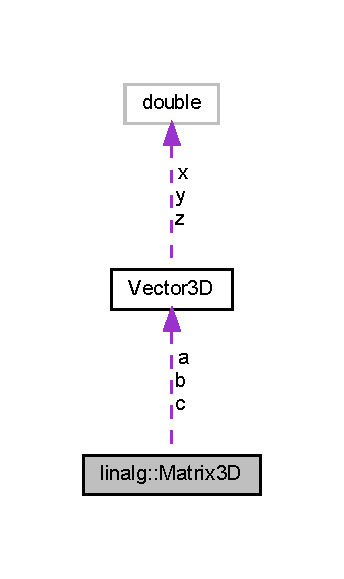
\includegraphics[width=165pt]{classlinalg_1_1Matrix3D__coll__graph}
\end{center}
\end{figure}
\subsection*{Public Member Functions}
\begin{DoxyCompactItemize}
\item 
\hyperlink{classlinalg_1_1Matrix3D_a868d0ba8d6ad2fcccc39c1633a5a854a}{Matrix3D} ()
\begin{DoxyCompactList}\small\item\em Constructs the identity matrix. \end{DoxyCompactList}\item 
\hyperlink{classlinalg_1_1Matrix3D_a3a7ce553d163d01e112c55a1afa712ca}{Matrix3D} (const \hyperlink{classVector3D}{Vector3D} \&\hyperlink{classlinalg_1_1Matrix3D_a33667283fe3c4bbac6d4f78eae2af3b6}{a}, const \hyperlink{classVector3D}{Vector3D} \&\hyperlink{classlinalg_1_1Matrix3D_acf0cd214420329fe18c902be95da0b23}{b}, const \hyperlink{classVector3D}{Vector3D} \&\hyperlink{classlinalg_1_1Matrix3D_abe82e945bf73f0d0f6f28c1749e2c7e3}{c})
\item 
double \& \hyperlink{classlinalg_1_1Matrix3D_a1021460c27da3f21690b68a2c7dea870}{at} (unsigned int i, unsigned int j)
\begin{DoxyCompactList}\small\item\em Returns a reference to the entry A\mbox{[}i, j\mbox{]} if the i and j are valid (i.\+e. 0$<$=i,j$<$3) \end{DoxyCompactList}\item 
const double \& \hyperlink{classlinalg_1_1Matrix3D_a2c5bee46e64a05d4671a8c72bc4f7e03}{at} (unsigned int i, unsigned int j) const 
\begin{DoxyCompactList}\small\item\em Returns a const reference to the entry A\mbox{[}i, j\mbox{]} if the i and j are valid (i.\+e. 0$<$=i,j$<$3) \end{DoxyCompactList}\item 
\hyperlink{classlinalg_1_1Matrix3D}{Matrix3D} \hyperlink{classlinalg_1_1Matrix3D_a45c2dfdae0a9a857e43429ac0fefa206}{transpose} () const 
\begin{DoxyCompactList}\small\item\em Returns the transpose of this matrix. \end{DoxyCompactList}\item 
\hyperlink{classlinalg_1_1Matrix3D}{Matrix3D} \& \hyperlink{classlinalg_1_1Matrix3D_aff9083d3f737113ea70ca544bee86d8f}{operator$\ast$=} (const \hyperlink{classlinalg_1_1Matrix3D}{Matrix3D} \&B)
\item 
\hyperlink{classlinalg_1_1Matrix3D}{Matrix3D} \& \hyperlink{classlinalg_1_1Matrix3D_ae9c4b93227bc3cb85796ae377a476d2b}{operator+=} (const \hyperlink{classlinalg_1_1Matrix3D}{Matrix3D} \&B)
\end{DoxyCompactItemize}
\subsection*{Private Attributes}
\begin{DoxyCompactItemize}
\item 
\hyperlink{classVector3D}{Vector3D} \hyperlink{classlinalg_1_1Matrix3D_a33667283fe3c4bbac6d4f78eae2af3b6}{a}
\begin{DoxyCompactList}\small\item\em The columns of the Matrix \mbox{[}a, b, c\mbox{]}. \end{DoxyCompactList}\item 
\hyperlink{classVector3D}{Vector3D} \hyperlink{classlinalg_1_1Matrix3D_acf0cd214420329fe18c902be95da0b23}{b}
\item 
\hyperlink{classVector3D}{Vector3D} \hyperlink{classlinalg_1_1Matrix3D_abe82e945bf73f0d0f6f28c1749e2c7e3}{c}
\end{DoxyCompactItemize}
\subsection*{Friends}
\begin{DoxyCompactItemize}
\item 
\hyperlink{classVector3D}{Vector3D} \hyperlink{classlinalg_1_1Matrix3D_a7ae064396881469e4d815cfba5804a2e}{operator$\ast$} (const \hyperlink{classlinalg_1_1Matrix3D}{Matrix3D} \&A, const \hyperlink{classVector3D}{Vector3D} \&v)
\item 
\hyperlink{classlinalg_1_1Matrix3D}{Matrix3D} \hyperlink{classlinalg_1_1Matrix3D_a701c3381ba551de2652b9f021a8454ec}{operator$\ast$} (\hyperlink{classlinalg_1_1Matrix3D}{Matrix3D} A, const \hyperlink{classlinalg_1_1Matrix3D}{Matrix3D} \&B)
\item 
\hyperlink{classlinalg_1_1Matrix3D}{Matrix3D} \hyperlink{classlinalg_1_1Matrix3D_a54929d88410f4beedd5ef7ef3ba8cffc}{operator+} (\hyperlink{classlinalg_1_1Matrix3D}{Matrix3D} A, const \hyperlink{classlinalg_1_1Matrix3D}{Matrix3D} \&B)
\end{DoxyCompactItemize}


\subsection{Detailed Description}
Square 3x3 Matrix. 

\subsection{Constructor \& Destructor Documentation}
\index{linalg\+::\+Matrix3D@{linalg\+::\+Matrix3D}!Matrix3D@{Matrix3D}}
\index{Matrix3D@{Matrix3D}!linalg\+::\+Matrix3D@{linalg\+::\+Matrix3D}}
\subsubsection[{\texorpdfstring{Matrix3\+D()}{Matrix3D()}}]{\setlength{\rightskip}{0pt plus 5cm}linalg\+::\+Matrix3\+D\+::\+Matrix3D (
\begin{DoxyParamCaption}
{}
\end{DoxyParamCaption}
)}\hypertarget{classlinalg_1_1Matrix3D_a868d0ba8d6ad2fcccc39c1633a5a854a}{}\label{classlinalg_1_1Matrix3D_a868d0ba8d6ad2fcccc39c1633a5a854a}


Constructs the identity matrix. 

\index{linalg\+::\+Matrix3D@{linalg\+::\+Matrix3D}!Matrix3D@{Matrix3D}}
\index{Matrix3D@{Matrix3D}!linalg\+::\+Matrix3D@{linalg\+::\+Matrix3D}}
\subsubsection[{\texorpdfstring{Matrix3\+D(const Vector3\+D \&a, const Vector3\+D \&b, const Vector3\+D \&c)}{Matrix3D(const Vector3D &a, const Vector3D &b, const Vector3D &c)}}]{\setlength{\rightskip}{0pt plus 5cm}linalg\+::\+Matrix3\+D\+::\+Matrix3D (
\begin{DoxyParamCaption}
\item[{const {\bf Vector3D} \&}]{a, }
\item[{const {\bf Vector3D} \&}]{b, }
\item[{const {\bf Vector3D} \&}]{c}
\end{DoxyParamCaption}
)\hspace{0.3cm}{\ttfamily [inline]}}\hypertarget{classlinalg_1_1Matrix3D_a3a7ce553d163d01e112c55a1afa712ca}{}\label{classlinalg_1_1Matrix3D_a3a7ce553d163d01e112c55a1afa712ca}


\subsection{Member Function Documentation}
\index{linalg\+::\+Matrix3D@{linalg\+::\+Matrix3D}!at@{at}}
\index{at@{at}!linalg\+::\+Matrix3D@{linalg\+::\+Matrix3D}}
\subsubsection[{\texorpdfstring{at(unsigned int i, unsigned int j)}{at(unsigned int i, unsigned int j)}}]{\setlength{\rightskip}{0pt plus 5cm}double \& linalg\+::\+Matrix3\+D\+::at (
\begin{DoxyParamCaption}
\item[{unsigned int}]{i, }
\item[{unsigned int}]{j}
\end{DoxyParamCaption}
)}\hypertarget{classlinalg_1_1Matrix3D_a1021460c27da3f21690b68a2c7dea870}{}\label{classlinalg_1_1Matrix3D_a1021460c27da3f21690b68a2c7dea870}


Returns a reference to the entry A\mbox{[}i, j\mbox{]} if the i and j are valid (i.\+e. 0$<$=i,j$<$3) 


\begin{DoxyParams}{Parameters}
{\em i} & The row \\
\hline
{\em j} & The column \\
\hline
\end{DoxyParams}
\begin{DoxyReturn}{Returns}
A reference to the entry in row i, column j 
\end{DoxyReturn}
\index{linalg\+::\+Matrix3D@{linalg\+::\+Matrix3D}!at@{at}}
\index{at@{at}!linalg\+::\+Matrix3D@{linalg\+::\+Matrix3D}}
\subsubsection[{\texorpdfstring{at(unsigned int i, unsigned int j) const }{at(unsigned int i, unsigned int j) const }}]{\setlength{\rightskip}{0pt plus 5cm}const double \& linalg\+::\+Matrix3\+D\+::at (
\begin{DoxyParamCaption}
\item[{unsigned int}]{i, }
\item[{unsigned int}]{j}
\end{DoxyParamCaption}
) const}\hypertarget{classlinalg_1_1Matrix3D_a2c5bee46e64a05d4671a8c72bc4f7e03}{}\label{classlinalg_1_1Matrix3D_a2c5bee46e64a05d4671a8c72bc4f7e03}


Returns a const reference to the entry A\mbox{[}i, j\mbox{]} if the i and j are valid (i.\+e. 0$<$=i,j$<$3) 


\begin{DoxyParams}{Parameters}
{\em i} & The row \\
\hline
{\em j} & The column \\
\hline
\end{DoxyParams}
\begin{DoxyReturn}{Returns}
A const reference to the entry in row i, column j 
\end{DoxyReturn}
\index{linalg\+::\+Matrix3D@{linalg\+::\+Matrix3D}!operator$\ast$=@{operator$\ast$=}}
\index{operator$\ast$=@{operator$\ast$=}!linalg\+::\+Matrix3D@{linalg\+::\+Matrix3D}}
\subsubsection[{\texorpdfstring{operator$\ast$=(const Matrix3\+D \&\+B)}{operator*=(const Matrix3D &B)}}]{\setlength{\rightskip}{0pt plus 5cm}{\bf Matrix3D} \& linalg\+::\+Matrix3\+D\+::operator$\ast$= (
\begin{DoxyParamCaption}
\item[{const {\bf Matrix3D} \&}]{B}
\end{DoxyParamCaption}
)}\hypertarget{classlinalg_1_1Matrix3D_aff9083d3f737113ea70ca544bee86d8f}{}\label{classlinalg_1_1Matrix3D_aff9083d3f737113ea70ca544bee86d8f}
\index{linalg\+::\+Matrix3D@{linalg\+::\+Matrix3D}!operator+=@{operator+=}}
\index{operator+=@{operator+=}!linalg\+::\+Matrix3D@{linalg\+::\+Matrix3D}}
\subsubsection[{\texorpdfstring{operator+=(const Matrix3\+D \&\+B)}{operator+=(const Matrix3D &B)}}]{\setlength{\rightskip}{0pt plus 5cm}{\bf Matrix3D} \& linalg\+::\+Matrix3\+D\+::operator+= (
\begin{DoxyParamCaption}
\item[{const {\bf Matrix3D} \&}]{B}
\end{DoxyParamCaption}
)}\hypertarget{classlinalg_1_1Matrix3D_ae9c4b93227bc3cb85796ae377a476d2b}{}\label{classlinalg_1_1Matrix3D_ae9c4b93227bc3cb85796ae377a476d2b}
\index{linalg\+::\+Matrix3D@{linalg\+::\+Matrix3D}!transpose@{transpose}}
\index{transpose@{transpose}!linalg\+::\+Matrix3D@{linalg\+::\+Matrix3D}}
\subsubsection[{\texorpdfstring{transpose() const }{transpose() const }}]{\setlength{\rightskip}{0pt plus 5cm}{\bf Matrix3D} linalg\+::\+Matrix3\+D\+::transpose (
\begin{DoxyParamCaption}
{}
\end{DoxyParamCaption}
) const}\hypertarget{classlinalg_1_1Matrix3D_a45c2dfdae0a9a857e43429ac0fefa206}{}\label{classlinalg_1_1Matrix3D_a45c2dfdae0a9a857e43429ac0fefa206}


Returns the transpose of this matrix. 

\begin{DoxyReturn}{Returns}
A.\+T if A is this matrix 
\end{DoxyReturn}


\subsection{Friends And Related Function Documentation}
\index{linalg\+::\+Matrix3D@{linalg\+::\+Matrix3D}!operator$\ast$@{operator$\ast$}}
\index{operator$\ast$@{operator$\ast$}!linalg\+::\+Matrix3D@{linalg\+::\+Matrix3D}}
\subsubsection[{\texorpdfstring{operator$\ast$}{operator*}}]{\setlength{\rightskip}{0pt plus 5cm}{\bf Vector3D} operator$\ast$ (
\begin{DoxyParamCaption}
\item[{const {\bf Matrix3D} \&}]{A, }
\item[{const {\bf Vector3D} \&}]{v}
\end{DoxyParamCaption}
)\hspace{0.3cm}{\ttfamily [friend]}}\hypertarget{classlinalg_1_1Matrix3D_a7ae064396881469e4d815cfba5804a2e}{}\label{classlinalg_1_1Matrix3D_a7ae064396881469e4d815cfba5804a2e}
\index{linalg\+::\+Matrix3D@{linalg\+::\+Matrix3D}!operator$\ast$@{operator$\ast$}}
\index{operator$\ast$@{operator$\ast$}!linalg\+::\+Matrix3D@{linalg\+::\+Matrix3D}}
\subsubsection[{\texorpdfstring{operator$\ast$}{operator*}}]{\setlength{\rightskip}{0pt plus 5cm}{\bf Matrix3D} operator$\ast$ (
\begin{DoxyParamCaption}
\item[{{\bf Matrix3D}}]{A, }
\item[{const {\bf Matrix3D} \&}]{B}
\end{DoxyParamCaption}
)\hspace{0.3cm}{\ttfamily [friend]}}\hypertarget{classlinalg_1_1Matrix3D_a701c3381ba551de2652b9f021a8454ec}{}\label{classlinalg_1_1Matrix3D_a701c3381ba551de2652b9f021a8454ec}
\index{linalg\+::\+Matrix3D@{linalg\+::\+Matrix3D}!operator+@{operator+}}
\index{operator+@{operator+}!linalg\+::\+Matrix3D@{linalg\+::\+Matrix3D}}
\subsubsection[{\texorpdfstring{operator+}{operator+}}]{\setlength{\rightskip}{0pt plus 5cm}{\bf Matrix3D} operator+ (
\begin{DoxyParamCaption}
\item[{{\bf Matrix3D}}]{A, }
\item[{const {\bf Matrix3D} \&}]{B}
\end{DoxyParamCaption}
)\hspace{0.3cm}{\ttfamily [friend]}}\hypertarget{classlinalg_1_1Matrix3D_a54929d88410f4beedd5ef7ef3ba8cffc}{}\label{classlinalg_1_1Matrix3D_a54929d88410f4beedd5ef7ef3ba8cffc}


\subsection{Member Data Documentation}
\index{linalg\+::\+Matrix3D@{linalg\+::\+Matrix3D}!a@{a}}
\index{a@{a}!linalg\+::\+Matrix3D@{linalg\+::\+Matrix3D}}
\subsubsection[{\texorpdfstring{a}{a}}]{\setlength{\rightskip}{0pt plus 5cm}{\bf Vector3D} linalg\+::\+Matrix3\+D\+::a\hspace{0.3cm}{\ttfamily [private]}}\hypertarget{classlinalg_1_1Matrix3D_a33667283fe3c4bbac6d4f78eae2af3b6}{}\label{classlinalg_1_1Matrix3D_a33667283fe3c4bbac6d4f78eae2af3b6}


The columns of the Matrix \mbox{[}a, b, c\mbox{]}. 

\index{linalg\+::\+Matrix3D@{linalg\+::\+Matrix3D}!b@{b}}
\index{b@{b}!linalg\+::\+Matrix3D@{linalg\+::\+Matrix3D}}
\subsubsection[{\texorpdfstring{b}{b}}]{\setlength{\rightskip}{0pt plus 5cm}{\bf Vector3D} linalg\+::\+Matrix3\+D\+::b\hspace{0.3cm}{\ttfamily [private]}}\hypertarget{classlinalg_1_1Matrix3D_acf0cd214420329fe18c902be95da0b23}{}\label{classlinalg_1_1Matrix3D_acf0cd214420329fe18c902be95da0b23}
\index{linalg\+::\+Matrix3D@{linalg\+::\+Matrix3D}!c@{c}}
\index{c@{c}!linalg\+::\+Matrix3D@{linalg\+::\+Matrix3D}}
\subsubsection[{\texorpdfstring{c}{c}}]{\setlength{\rightskip}{0pt plus 5cm}{\bf Vector3D} linalg\+::\+Matrix3\+D\+::c\hspace{0.3cm}{\ttfamily [private]}}\hypertarget{classlinalg_1_1Matrix3D_abe82e945bf73f0d0f6f28c1749e2c7e3}{}\label{classlinalg_1_1Matrix3D_abe82e945bf73f0d0f6f28c1749e2c7e3}


The documentation for this class was generated from the following files\+:\begin{DoxyCompactItemize}
\item 
src/linalg/\hyperlink{Matrix3D_8h}{Matrix3\+D.\+h}\item 
src/linalg/\hyperlink{Matrix3D_8cpp}{Matrix3\+D.\+cpp}\end{DoxyCompactItemize}

\hypertarget{classMTLLib}{}\section{M\+T\+L\+Lib Class Reference}
\label{classMTLLib}\index{M\+T\+L\+Lib@{M\+T\+L\+Lib}}


Class for loading wavefront .mtl files.  




{\ttfamily \#include $<$M\+T\+L\+Lib.\+h$>$}



Collaboration diagram for M\+T\+L\+Lib\+:\nopagebreak
\begin{figure}[H]
\begin{center}
\leavevmode
\includegraphics[width=186pt]{classMTLLib__coll__graph}
\end{center}
\end{figure}
\subsection*{Public Member Functions}
\begin{DoxyCompactItemize}
\item 
\hyperlink{classMTLLib_a9d67275ad7ced3768135bd40bc821616}{M\+T\+L\+Lib} (const char $\ast$filename)
\item 
\hyperlink{classMTLLib_a1f6320f63cdc48012b12b993ce74777c}{M\+T\+L\+Lib} ()=default
\item 
bool \hyperlink{classMTLLib_a7c7743ed1a557874d470f8bc7946801f}{contains} (std\+::string key) const 
\item 
\hyperlink{classMaterial}{Material} \& \hyperlink{classMTLLib_a47584cec05a84d6b173c655515788b76}{operator\mbox{[}$\,$\mbox{]}} (std\+::string key)
\item 
std\+::ostream \& \hyperlink{classMTLLib_a9c5381e22b3572af42e7b23335ea8074}{print} (std\+::ostream \&sink) const 
\end{DoxyCompactItemize}
\subsection*{Private Attributes}
\begin{DoxyCompactItemize}
\item 
std\+::unordered\+\_\+map$<$ std\+::string, \hyperlink{classMaterial}{Material} $>$ \hyperlink{classMTLLib_aff9c5fb2df226fe6c383ed8faaf9e49d}{materials}
\end{DoxyCompactItemize}
\subsection*{Friends}
\begin{DoxyCompactItemize}
\item 
std\+::ostream \& \hyperlink{classMTLLib_a8827df67313eff58b309533133a8f437}{operator$<$$<$} (std\+::ostream \&sink, const \hyperlink{classMTLLib}{M\+T\+L\+Lib} \&lib)
\end{DoxyCompactItemize}


\subsection{Detailed Description}
Class for loading wavefront .mtl files. 

\subsection{Constructor \& Destructor Documentation}
\index{M\+T\+L\+Lib@{M\+T\+L\+Lib}!M\+T\+L\+Lib@{M\+T\+L\+Lib}}
\index{M\+T\+L\+Lib@{M\+T\+L\+Lib}!M\+T\+L\+Lib@{M\+T\+L\+Lib}}
\subsubsection[{\texorpdfstring{M\+T\+L\+Lib(const char $\ast$filename)}{MTLLib(const char *filename)}}]{\setlength{\rightskip}{0pt plus 5cm}M\+T\+L\+Lib\+::\+M\+T\+L\+Lib (
\begin{DoxyParamCaption}
\item[{const char $\ast$}]{filename}
\end{DoxyParamCaption}
)\hspace{0.3cm}{\ttfamily [explicit]}}\hypertarget{classMTLLib_a9d67275ad7ced3768135bd40bc821616}{}\label{classMTLLib_a9d67275ad7ced3768135bd40bc821616}
\index{M\+T\+L\+Lib@{M\+T\+L\+Lib}!M\+T\+L\+Lib@{M\+T\+L\+Lib}}
\index{M\+T\+L\+Lib@{M\+T\+L\+Lib}!M\+T\+L\+Lib@{M\+T\+L\+Lib}}
\subsubsection[{\texorpdfstring{M\+T\+L\+Lib()=default}{MTLLib()=default}}]{\setlength{\rightskip}{0pt plus 5cm}M\+T\+L\+Lib\+::\+M\+T\+L\+Lib (
\begin{DoxyParamCaption}
{}
\end{DoxyParamCaption}
)\hspace{0.3cm}{\ttfamily [default]}}\hypertarget{classMTLLib_a1f6320f63cdc48012b12b993ce74777c}{}\label{classMTLLib_a1f6320f63cdc48012b12b993ce74777c}


\subsection{Member Function Documentation}
\index{M\+T\+L\+Lib@{M\+T\+L\+Lib}!contains@{contains}}
\index{contains@{contains}!M\+T\+L\+Lib@{M\+T\+L\+Lib}}
\subsubsection[{\texorpdfstring{contains(std\+::string key) const }{contains(std::string key) const }}]{\setlength{\rightskip}{0pt plus 5cm}bool M\+T\+L\+Lib\+::contains (
\begin{DoxyParamCaption}
\item[{std\+::string}]{key}
\end{DoxyParamCaption}
) const}\hypertarget{classMTLLib_a7c7743ed1a557874d470f8bc7946801f}{}\label{classMTLLib_a7c7743ed1a557874d470f8bc7946801f}
\index{M\+T\+L\+Lib@{M\+T\+L\+Lib}!operator\mbox{[}$\,$\mbox{]}@{operator[]}}
\index{operator\mbox{[}$\,$\mbox{]}@{operator[]}!M\+T\+L\+Lib@{M\+T\+L\+Lib}}
\subsubsection[{\texorpdfstring{operator[](std\+::string key)}{operator[](std::string key)}}]{\setlength{\rightskip}{0pt plus 5cm}{\bf Material} \& M\+T\+L\+Lib\+::operator\mbox{[}$\,$\mbox{]} (
\begin{DoxyParamCaption}
\item[{std\+::string}]{key}
\end{DoxyParamCaption}
)}\hypertarget{classMTLLib_a47584cec05a84d6b173c655515788b76}{}\label{classMTLLib_a47584cec05a84d6b173c655515788b76}
\index{M\+T\+L\+Lib@{M\+T\+L\+Lib}!print@{print}}
\index{print@{print}!M\+T\+L\+Lib@{M\+T\+L\+Lib}}
\subsubsection[{\texorpdfstring{print(std\+::ostream \&sink) const }{print(std::ostream &sink) const }}]{\setlength{\rightskip}{0pt plus 5cm}std\+::ostream \& M\+T\+L\+Lib\+::print (
\begin{DoxyParamCaption}
\item[{std\+::ostream \&}]{sink}
\end{DoxyParamCaption}
) const}\hypertarget{classMTLLib_a9c5381e22b3572af42e7b23335ea8074}{}\label{classMTLLib_a9c5381e22b3572af42e7b23335ea8074}


\subsection{Friends And Related Function Documentation}
\index{M\+T\+L\+Lib@{M\+T\+L\+Lib}!operator$<$$<$@{operator$<$$<$}}
\index{operator$<$$<$@{operator$<$$<$}!M\+T\+L\+Lib@{M\+T\+L\+Lib}}
\subsubsection[{\texorpdfstring{operator$<$$<$}{operator<<}}]{\setlength{\rightskip}{0pt plus 5cm}std\+::ostream\& operator$<$$<$ (
\begin{DoxyParamCaption}
\item[{std\+::ostream \&}]{sink, }
\item[{const {\bf M\+T\+L\+Lib} \&}]{lib}
\end{DoxyParamCaption}
)\hspace{0.3cm}{\ttfamily [friend]}}\hypertarget{classMTLLib_a8827df67313eff58b309533133a8f437}{}\label{classMTLLib_a8827df67313eff58b309533133a8f437}


\subsection{Member Data Documentation}
\index{M\+T\+L\+Lib@{M\+T\+L\+Lib}!materials@{materials}}
\index{materials@{materials}!M\+T\+L\+Lib@{M\+T\+L\+Lib}}
\subsubsection[{\texorpdfstring{materials}{materials}}]{\setlength{\rightskip}{0pt plus 5cm}std\+::unordered\+\_\+map$<$std\+::string, {\bf Material}$>$ M\+T\+L\+Lib\+::materials\hspace{0.3cm}{\ttfamily [private]}}\hypertarget{classMTLLib_aff9c5fb2df226fe6c383ed8faaf9e49d}{}\label{classMTLLib_aff9c5fb2df226fe6c383ed8faaf9e49d}


The documentation for this class was generated from the following files\+:\begin{DoxyCompactItemize}
\item 
src/\hyperlink{MTLLib_8h}{M\+T\+L\+Lib.\+h}\item 
src/\hyperlink{MTLLib_8cpp}{M\+T\+L\+Lib.\+cpp}\end{DoxyCompactItemize}

\hypertarget{classsymcpp_1_1Multiply}{}\section{symcpp\+:\+:Multiply Class Reference}
\label{classsymcpp_1_1Multiply}\index{symcpp\+::\+Multiply@{symcpp\+::\+Multiply}}


{\ttfamily \#include $<$Multiply.\+h$>$}



Inheritance diagram for symcpp\+:\+:Multiply\+:\nopagebreak
\begin{figure}[H]
\begin{center}
\leavevmode
\includegraphics[width=186pt]{classsymcpp_1_1Multiply__inherit__graph}
\end{center}
\end{figure}


Collaboration diagram for symcpp\+:\+:Multiply\+:\nopagebreak
\begin{figure}[H]
\begin{center}
\leavevmode
\includegraphics[width=310pt]{classsymcpp_1_1Multiply__coll__graph}
\end{center}
\end{figure}
\subsection*{Public Member Functions}
\begin{DoxyCompactItemize}
\item 
\hyperlink{classsymcpp_1_1Multiply_abe8b88c2ac3ecd7deb275b1cb1f5dd9d}{Multiply} (const \hyperlink{classsymcpp_1_1Expression}{Expression} \&\hyperlink{classsymcpp_1_1Multiply_a8ed32ccb235cea51161dd0fd25ea130d}{a}, const \hyperlink{classsymcpp_1_1Expression}{Expression} \&\hyperlink{classsymcpp_1_1Multiply_a3d7a1b6e6e35585098b25f8b3a59e6ae}{b})
\item 
\hyperlink{classsymcpp_1_1Multiply_abefbdc2703e4c56207fe9aa987097fe6}{Multiply} (std\+::unique\+\_\+ptr$<$ \hyperlink{classsymcpp_1_1Expression}{Expression} $>$ \&\&\hyperlink{classsymcpp_1_1Multiply_a8ed32ccb235cea51161dd0fd25ea130d}{a}, std\+::unique\+\_\+ptr$<$ \hyperlink{classsymcpp_1_1Expression}{Expression} $>$ \&\&\hyperlink{classsymcpp_1_1Multiply_a3d7a1b6e6e35585098b25f8b3a59e6ae}{b})
\item 
std\+::unique\+\_\+ptr$<$ \hyperlink{classsymcpp_1_1Expression}{Expression} $>$ \hyperlink{classsymcpp_1_1Multiply_adcd57ab1c1a27eb10aeeb572cdd14e5e}{copy} () const override
\item 
std\+::unique\+\_\+ptr$<$ \hyperlink{classsymcpp_1_1Expression}{Expression} $>$ \hyperlink{classsymcpp_1_1Multiply_a835e55ada54a6c1eeb6d02ceeef83198}{diff} (std\+::string v) const override
\item 
double \hyperlink{classsymcpp_1_1Multiply_a83a9396b931cd5010630f48ecd1bc2a1}{subs} (const std\+::unordered\+\_\+map$<$ std\+::string, double $>$ \&env) const override
\item 
unsigned int \hyperlink{classsymcpp_1_1Multiply_afd9f779b82aa2d7a3be63e7b8b0e8eb1}{precedence} () const override
\item 
bool \hyperlink{classsymcpp_1_1Multiply_a771fc25f8bafd49600c31db11dd72256}{is\+\_\+constant} () const override
\item 
std\+::unique\+\_\+ptr$<$ \hyperlink{classsymcpp_1_1Expression}{Expression} $>$ \hyperlink{classsymcpp_1_1Multiply_aff728e2edaa447f154918079b4e35a7e}{simplify} () override
\item 
double \hyperlink{classsymcpp_1_1Multiply_a1d9b8023ab0bf35c011eb7f3ee8d4c32}{const\+\_\+eval} () const override
\end{DoxyCompactItemize}
\subsection*{Private Member Functions}
\begin{DoxyCompactItemize}
\item 
std\+::ostream \& \hyperlink{classsymcpp_1_1Multiply_a8d6dbfc85d0609f40d52c0fc853a06b5}{print} (std\+::ostream \&sink) const override
\end{DoxyCompactItemize}
\subsection*{Private Attributes}
\begin{DoxyCompactItemize}
\item 
std\+::unique\+\_\+ptr$<$ \hyperlink{classsymcpp_1_1Expression}{Expression} $>$ \hyperlink{classsymcpp_1_1Multiply_a8ed32ccb235cea51161dd0fd25ea130d}{a}
\item 
std\+::unique\+\_\+ptr$<$ \hyperlink{classsymcpp_1_1Expression}{Expression} $>$ \hyperlink{classsymcpp_1_1Multiply_a3d7a1b6e6e35585098b25f8b3a59e6ae}{b}
\end{DoxyCompactItemize}


\subsection{Constructor \& Destructor Documentation}
\index{symcpp\+::\+Multiply@{symcpp\+::\+Multiply}!Multiply@{Multiply}}
\index{Multiply@{Multiply}!symcpp\+::\+Multiply@{symcpp\+::\+Multiply}}
\subsubsection[{\texorpdfstring{Multiply(const Expression \&a, const Expression \&b)}{Multiply(const Expression &a, const Expression &b)}}]{\setlength{\rightskip}{0pt plus 5cm}symcpp\+::\+Multiply\+::\+Multiply (
\begin{DoxyParamCaption}
\item[{const {\bf Expression} \&}]{a, }
\item[{const {\bf Expression} \&}]{b}
\end{DoxyParamCaption}
)}\hypertarget{classsymcpp_1_1Multiply_abe8b88c2ac3ecd7deb275b1cb1f5dd9d}{}\label{classsymcpp_1_1Multiply_abe8b88c2ac3ecd7deb275b1cb1f5dd9d}
\index{symcpp\+::\+Multiply@{symcpp\+::\+Multiply}!Multiply@{Multiply}}
\index{Multiply@{Multiply}!symcpp\+::\+Multiply@{symcpp\+::\+Multiply}}
\subsubsection[{\texorpdfstring{Multiply(std\+::unique\+\_\+ptr$<$ Expression $>$ \&\&a, std\+::unique\+\_\+ptr$<$ Expression $>$ \&\&b)}{Multiply(std::unique_ptr< Expression > &&a, std::unique_ptr< Expression > &&b)}}]{\setlength{\rightskip}{0pt plus 5cm}symcpp\+::\+Multiply\+::\+Multiply (
\begin{DoxyParamCaption}
\item[{std\+::unique\+\_\+ptr$<$ {\bf Expression} $>$ \&\&}]{a, }
\item[{std\+::unique\+\_\+ptr$<$ {\bf Expression} $>$ \&\&}]{b}
\end{DoxyParamCaption}
)}\hypertarget{classsymcpp_1_1Multiply_abefbdc2703e4c56207fe9aa987097fe6}{}\label{classsymcpp_1_1Multiply_abefbdc2703e4c56207fe9aa987097fe6}


\subsection{Member Function Documentation}
\index{symcpp\+::\+Multiply@{symcpp\+::\+Multiply}!const\+\_\+eval@{const\+\_\+eval}}
\index{const\+\_\+eval@{const\+\_\+eval}!symcpp\+::\+Multiply@{symcpp\+::\+Multiply}}
\subsubsection[{\texorpdfstring{const\+\_\+eval() const override}{const_eval() const override}}]{\setlength{\rightskip}{0pt plus 5cm}double symcpp\+::\+Multiply\+::const\+\_\+eval (
\begin{DoxyParamCaption}
{}
\end{DoxyParamCaption}
) const\hspace{0.3cm}{\ttfamily [override]}, {\ttfamily [virtual]}}\hypertarget{classsymcpp_1_1Multiply_a1d9b8023ab0bf35c011eb7f3ee8d4c32}{}\label{classsymcpp_1_1Multiply_a1d9b8023ab0bf35c011eb7f3ee8d4c32}


Implements \hyperlink{classsymcpp_1_1Expression_a81c8069347f586cb5632338d97c278ad}{symcpp\+::\+Expression}.

\index{symcpp\+::\+Multiply@{symcpp\+::\+Multiply}!copy@{copy}}
\index{copy@{copy}!symcpp\+::\+Multiply@{symcpp\+::\+Multiply}}
\subsubsection[{\texorpdfstring{copy() const override}{copy() const override}}]{\setlength{\rightskip}{0pt plus 5cm}std\+::unique\+\_\+ptr$<$ {\bf Expression} $>$ symcpp\+::\+Multiply\+::copy (
\begin{DoxyParamCaption}
{}
\end{DoxyParamCaption}
) const\hspace{0.3cm}{\ttfamily [override]}, {\ttfamily [virtual]}}\hypertarget{classsymcpp_1_1Multiply_adcd57ab1c1a27eb10aeeb572cdd14e5e}{}\label{classsymcpp_1_1Multiply_adcd57ab1c1a27eb10aeeb572cdd14e5e}


Implements \hyperlink{classsymcpp_1_1Expression_a2e7de5a295ccf0efdc9b34cea7ba3d0b}{symcpp\+::\+Expression}.

\index{symcpp\+::\+Multiply@{symcpp\+::\+Multiply}!diff@{diff}}
\index{diff@{diff}!symcpp\+::\+Multiply@{symcpp\+::\+Multiply}}
\subsubsection[{\texorpdfstring{diff(std\+::string v) const override}{diff(std::string v) const override}}]{\setlength{\rightskip}{0pt plus 5cm}std\+::unique\+\_\+ptr$<$ {\bf Expression} $>$ symcpp\+::\+Multiply\+::diff (
\begin{DoxyParamCaption}
\item[{std\+::string}]{v}
\end{DoxyParamCaption}
) const\hspace{0.3cm}{\ttfamily [override]}, {\ttfamily [virtual]}}\hypertarget{classsymcpp_1_1Multiply_a835e55ada54a6c1eeb6d02ceeef83198}{}\label{classsymcpp_1_1Multiply_a835e55ada54a6c1eeb6d02ceeef83198}


Implements \hyperlink{classsymcpp_1_1Expression_a032fe8da79d5e231ca2d21a201c8f32d}{symcpp\+::\+Expression}.

\index{symcpp\+::\+Multiply@{symcpp\+::\+Multiply}!is\+\_\+constant@{is\+\_\+constant}}
\index{is\+\_\+constant@{is\+\_\+constant}!symcpp\+::\+Multiply@{symcpp\+::\+Multiply}}
\subsubsection[{\texorpdfstring{is\+\_\+constant() const override}{is_constant() const override}}]{\setlength{\rightskip}{0pt plus 5cm}bool symcpp\+::\+Multiply\+::is\+\_\+constant (
\begin{DoxyParamCaption}
{}
\end{DoxyParamCaption}
) const\hspace{0.3cm}{\ttfamily [override]}, {\ttfamily [virtual]}}\hypertarget{classsymcpp_1_1Multiply_a771fc25f8bafd49600c31db11dd72256}{}\label{classsymcpp_1_1Multiply_a771fc25f8bafd49600c31db11dd72256}


Implements \hyperlink{classsymcpp_1_1Expression_a30db7917c8948e22330cbe8259caeae2}{symcpp\+::\+Expression}.

\index{symcpp\+::\+Multiply@{symcpp\+::\+Multiply}!precedence@{precedence}}
\index{precedence@{precedence}!symcpp\+::\+Multiply@{symcpp\+::\+Multiply}}
\subsubsection[{\texorpdfstring{precedence() const override}{precedence() const override}}]{\setlength{\rightskip}{0pt plus 5cm}unsigned int symcpp\+::\+Multiply\+::precedence (
\begin{DoxyParamCaption}
{}
\end{DoxyParamCaption}
) const\hspace{0.3cm}{\ttfamily [override]}, {\ttfamily [virtual]}}\hypertarget{classsymcpp_1_1Multiply_afd9f779b82aa2d7a3be63e7b8b0e8eb1}{}\label{classsymcpp_1_1Multiply_afd9f779b82aa2d7a3be63e7b8b0e8eb1}


Implements \hyperlink{classsymcpp_1_1Expression_a181c162d5740faac392ffdca26bfca0c}{symcpp\+::\+Expression}.

\index{symcpp\+::\+Multiply@{symcpp\+::\+Multiply}!print@{print}}
\index{print@{print}!symcpp\+::\+Multiply@{symcpp\+::\+Multiply}}
\subsubsection[{\texorpdfstring{print(std\+::ostream \&sink) const override}{print(std::ostream &sink) const override}}]{\setlength{\rightskip}{0pt plus 5cm}std\+::ostream \& symcpp\+::\+Multiply\+::print (
\begin{DoxyParamCaption}
\item[{std\+::ostream \&}]{sink}
\end{DoxyParamCaption}
) const\hspace{0.3cm}{\ttfamily [override]}, {\ttfamily [private]}, {\ttfamily [virtual]}}\hypertarget{classsymcpp_1_1Multiply_a8d6dbfc85d0609f40d52c0fc853a06b5}{}\label{classsymcpp_1_1Multiply_a8d6dbfc85d0609f40d52c0fc853a06b5}


Implements \hyperlink{classsymcpp_1_1Expression_af37e13032a40f2da4d2866eaa8658049}{symcpp\+::\+Expression}.

\index{symcpp\+::\+Multiply@{symcpp\+::\+Multiply}!simplify@{simplify}}
\index{simplify@{simplify}!symcpp\+::\+Multiply@{symcpp\+::\+Multiply}}
\subsubsection[{\texorpdfstring{simplify() override}{simplify() override}}]{\setlength{\rightskip}{0pt plus 5cm}std\+::unique\+\_\+ptr$<$ {\bf Expression} $>$ symcpp\+::\+Multiply\+::simplify (
\begin{DoxyParamCaption}
{}
\end{DoxyParamCaption}
)\hspace{0.3cm}{\ttfamily [override]}, {\ttfamily [virtual]}}\hypertarget{classsymcpp_1_1Multiply_aff728e2edaa447f154918079b4e35a7e}{}\label{classsymcpp_1_1Multiply_aff728e2edaa447f154918079b4e35a7e}


Implements \hyperlink{classsymcpp_1_1Expression_ab1fa6e55eea0682250d013f28db26cd2}{symcpp\+::\+Expression}.

\index{symcpp\+::\+Multiply@{symcpp\+::\+Multiply}!subs@{subs}}
\index{subs@{subs}!symcpp\+::\+Multiply@{symcpp\+::\+Multiply}}
\subsubsection[{\texorpdfstring{subs(const std\+::unordered\+\_\+map$<$ std\+::string, double $>$ \&env) const override}{subs(const std::unordered_map< std::string, double > &env) const override}}]{\setlength{\rightskip}{0pt plus 5cm}double symcpp\+::\+Multiply\+::subs (
\begin{DoxyParamCaption}
\item[{const std\+::unordered\+\_\+map$<$ std\+::string, double $>$ \&}]{env}
\end{DoxyParamCaption}
) const\hspace{0.3cm}{\ttfamily [override]}, {\ttfamily [virtual]}}\hypertarget{classsymcpp_1_1Multiply_a83a9396b931cd5010630f48ecd1bc2a1}{}\label{classsymcpp_1_1Multiply_a83a9396b931cd5010630f48ecd1bc2a1}


Implements \hyperlink{classsymcpp_1_1Expression_aaef29b0afa2d6c21fe35f47a1be76134}{symcpp\+::\+Expression}.



\subsection{Member Data Documentation}
\index{symcpp\+::\+Multiply@{symcpp\+::\+Multiply}!a@{a}}
\index{a@{a}!symcpp\+::\+Multiply@{symcpp\+::\+Multiply}}
\subsubsection[{\texorpdfstring{a}{a}}]{\setlength{\rightskip}{0pt plus 5cm}std\+::unique\+\_\+ptr$<${\bf Expression}$>$ symcpp\+::\+Multiply\+::a\hspace{0.3cm}{\ttfamily [private]}}\hypertarget{classsymcpp_1_1Multiply_a8ed32ccb235cea51161dd0fd25ea130d}{}\label{classsymcpp_1_1Multiply_a8ed32ccb235cea51161dd0fd25ea130d}
\index{symcpp\+::\+Multiply@{symcpp\+::\+Multiply}!b@{b}}
\index{b@{b}!symcpp\+::\+Multiply@{symcpp\+::\+Multiply}}
\subsubsection[{\texorpdfstring{b}{b}}]{\setlength{\rightskip}{0pt plus 5cm}std\+::unique\+\_\+ptr$<${\bf Expression}$>$ symcpp\+::\+Multiply\+::b\hspace{0.3cm}{\ttfamily [private]}}\hypertarget{classsymcpp_1_1Multiply_a3d7a1b6e6e35585098b25f8b3a59e6ae}{}\label{classsymcpp_1_1Multiply_a3d7a1b6e6e35585098b25f8b3a59e6ae}


The documentation for this class was generated from the following files\+:\begin{DoxyCompactItemize}
\item 
src/symcpp/\hyperlink{Multiply_8h}{Multiply.\+h}\item 
src/symcpp/\hyperlink{Multiply_8cpp}{Multiply.\+cpp}\end{DoxyCompactItemize}

\hypertarget{classOBJFile}{}\section{O\+B\+J\+File Class Reference}
\label{classOBJFile}\index{OBJFile@{OBJFile}}


Class for loading wavefront .obj files.  




{\ttfamily \#include $<$O\+B\+J\+File.\+h$>$}



Collaboration diagram for O\+B\+J\+File\+:
\nopagebreak
\begin{figure}[H]
\begin{center}
\leavevmode
\includegraphics[width=350pt]{classOBJFile__coll__graph}
\end{center}
\end{figure}
\subsection*{Public Member Functions}
\begin{DoxyCompactItemize}
\item 
\mbox{\hyperlink{classOBJFile_ac6c14cded889593868aaab4e7d3e4bfb}{O\+B\+J\+File}} (const char $\ast$file\+\_\+name, \mbox{\hyperlink{classMaterial}{Material}} mat)
\item 
std\+::vector$<$ \mbox{\hyperlink{classTriangle}{Triangle}} $>$ \mbox{\hyperlink{classOBJFile_a109fb06479ee891b78401e95e8b5b64e}{get\+\_\+triangles}} () const
\item 
void \mbox{\hyperlink{classOBJFile_adb2b2bb5e0a2920a2886272a1c9ebdab}{dump}} (std\+::string file\+\_\+name) const
\item 
\mbox{\hyperlink{classBinaryVolumeHierarchy}{Binary\+Volume\+Hierarchy}} \mbox{\hyperlink{classOBJFile_ae3128b473a8b7b837364cc9688cb89dc}{get\+B\+VH}} ()
\end{DoxyCompactItemize}
\subsection*{Private Attributes}
\begin{DoxyCompactItemize}
\item 
std\+::vector$<$ \mbox{\hyperlink{classTriangle}{Triangle}} $>$ \mbox{\hyperlink{classOBJFile_a7d568b98c43fd96142d9f0f0e57b296e}{polygons}}
\item 
std\+::vector$<$ \mbox{\hyperlink{classVector3D}{Vector3D}} $>$ \mbox{\hyperlink{classOBJFile_a9b07010eef35e7d44250f5f4f8fa3428}{vertices}}
\item 
std\+::vector$<$ \mbox{\hyperlink{classVector3D}{Vector3D}} $>$ \mbox{\hyperlink{classOBJFile_a287bef6fc146d20df4585d103b226eec}{normals}}
\item 
\mbox{\hyperlink{classMTLLib}{M\+T\+L\+Lib}} \mbox{\hyperlink{classOBJFile_a5b08a58ba3f59a931eea6067e29f3e40}{materials}}
\end{DoxyCompactItemize}


\subsection{Detailed Description}
Class for loading wavefront .obj files. 

\subsection{Constructor \& Destructor Documentation}
\mbox{\Hypertarget{classOBJFile_ac6c14cded889593868aaab4e7d3e4bfb}\label{classOBJFile_ac6c14cded889593868aaab4e7d3e4bfb}} 
\index{OBJFile@{OBJFile}!OBJFile@{OBJFile}}
\index{OBJFile@{OBJFile}!OBJFile@{OBJFile}}
\subsubsection{\texorpdfstring{OBJFile()}{OBJFile()}}
{\footnotesize\ttfamily O\+B\+J\+File\+::\+O\+B\+J\+File (\begin{DoxyParamCaption}\item[{const char $\ast$}]{file\+\_\+name,  }\item[{\mbox{\hyperlink{classMaterial}{Material}}}]{mat }\end{DoxyParamCaption})}



\subsection{Member Function Documentation}
\mbox{\Hypertarget{classOBJFile_adb2b2bb5e0a2920a2886272a1c9ebdab}\label{classOBJFile_adb2b2bb5e0a2920a2886272a1c9ebdab}} 
\index{OBJFile@{OBJFile}!dump@{dump}}
\index{dump@{dump}!OBJFile@{OBJFile}}
\subsubsection{\texorpdfstring{dump()}{dump()}}
{\footnotesize\ttfamily void O\+B\+J\+File\+::dump (\begin{DoxyParamCaption}\item[{std\+::string}]{file\+\_\+name }\end{DoxyParamCaption}) const}

\mbox{\Hypertarget{classOBJFile_a109fb06479ee891b78401e95e8b5b64e}\label{classOBJFile_a109fb06479ee891b78401e95e8b5b64e}} 
\index{OBJFile@{OBJFile}!get\_triangles@{get\_triangles}}
\index{get\_triangles@{get\_triangles}!OBJFile@{OBJFile}}
\subsubsection{\texorpdfstring{get\_triangles()}{get\_triangles()}}
{\footnotesize\ttfamily std\+::vector$<$ \mbox{\hyperlink{classTriangle}{Triangle}} $>$ O\+B\+J\+File\+::get\+\_\+triangles (\begin{DoxyParamCaption}{ }\end{DoxyParamCaption}) const}

\mbox{\Hypertarget{classOBJFile_ae3128b473a8b7b837364cc9688cb89dc}\label{classOBJFile_ae3128b473a8b7b837364cc9688cb89dc}} 
\index{OBJFile@{OBJFile}!getBVH@{getBVH}}
\index{getBVH@{getBVH}!OBJFile@{OBJFile}}
\subsubsection{\texorpdfstring{getBVH()}{getBVH()}}
{\footnotesize\ttfamily \mbox{\hyperlink{classBinaryVolumeHierarchy}{Binary\+Volume\+Hierarchy}} O\+B\+J\+File\+::get\+B\+VH (\begin{DoxyParamCaption}{ }\end{DoxyParamCaption})}



\subsection{Member Data Documentation}
\mbox{\Hypertarget{classOBJFile_a5b08a58ba3f59a931eea6067e29f3e40}\label{classOBJFile_a5b08a58ba3f59a931eea6067e29f3e40}} 
\index{OBJFile@{OBJFile}!materials@{materials}}
\index{materials@{materials}!OBJFile@{OBJFile}}
\subsubsection{\texorpdfstring{materials}{materials}}
{\footnotesize\ttfamily \mbox{\hyperlink{classMTLLib}{M\+T\+L\+Lib}} O\+B\+J\+File\+::materials\hspace{0.3cm}{\ttfamily [private]}}

\mbox{\Hypertarget{classOBJFile_a287bef6fc146d20df4585d103b226eec}\label{classOBJFile_a287bef6fc146d20df4585d103b226eec}} 
\index{OBJFile@{OBJFile}!normals@{normals}}
\index{normals@{normals}!OBJFile@{OBJFile}}
\subsubsection{\texorpdfstring{normals}{normals}}
{\footnotesize\ttfamily std\+::vector$<$\mbox{\hyperlink{classVector3D}{Vector3D}}$>$ O\+B\+J\+File\+::normals\hspace{0.3cm}{\ttfamily [private]}}

\mbox{\Hypertarget{classOBJFile_a7d568b98c43fd96142d9f0f0e57b296e}\label{classOBJFile_a7d568b98c43fd96142d9f0f0e57b296e}} 
\index{OBJFile@{OBJFile}!polygons@{polygons}}
\index{polygons@{polygons}!OBJFile@{OBJFile}}
\subsubsection{\texorpdfstring{polygons}{polygons}}
{\footnotesize\ttfamily std\+::vector$<$\mbox{\hyperlink{classTriangle}{Triangle}}$>$ O\+B\+J\+File\+::polygons\hspace{0.3cm}{\ttfamily [private]}}

\mbox{\Hypertarget{classOBJFile_a9b07010eef35e7d44250f5f4f8fa3428}\label{classOBJFile_a9b07010eef35e7d44250f5f4f8fa3428}} 
\index{OBJFile@{OBJFile}!vertices@{vertices}}
\index{vertices@{vertices}!OBJFile@{OBJFile}}
\subsubsection{\texorpdfstring{vertices}{vertices}}
{\footnotesize\ttfamily std\+::vector$<$\mbox{\hyperlink{classVector3D}{Vector3D}}$>$ O\+B\+J\+File\+::vertices\hspace{0.3cm}{\ttfamily [private]}}



The documentation for this class was generated from the following files\+:\begin{DoxyCompactItemize}
\item 
src/\mbox{\hyperlink{OBJFile_8h}{O\+B\+J\+File.\+h}}\item 
src/\mbox{\hyperlink{OBJFile_8cpp}{O\+B\+J\+File.\+cpp}}\end{DoxyCompactItemize}

\hypertarget{classcamera_1_1PinHoleCamera}{}\section{camera\+:\+:Pin\+Hole\+Camera Class Reference}
\label{classcamera_1_1PinHoleCamera}\index{camera\+::\+Pin\+Hole\+Camera@{camera\+::\+Pin\+Hole\+Camera}}


Implementation of \hyperlink{classcamera_1_1Camera}{Camera} class.  




{\ttfamily \#include $<$Pin\+Hole\+Camera.\+h$>$}



Inheritance diagram for camera\+:\+:Pin\+Hole\+Camera\+:\nopagebreak
\begin{figure}[H]
\begin{center}
\leavevmode
\includegraphics[width=204pt]{classcamera_1_1PinHoleCamera__inherit__graph}
\end{center}
\end{figure}


Collaboration diagram for camera\+:\+:Pin\+Hole\+Camera\+:\nopagebreak
\begin{figure}[H]
\begin{center}
\leavevmode
\includegraphics[width=324pt]{classcamera_1_1PinHoleCamera__coll__graph}
\end{center}
\end{figure}
\subsection*{Public Member Functions}
\begin{DoxyCompactItemize}
\item 
\hyperlink{classcamera_1_1PinHoleCamera_a0d7c74abd23ababb8e244fade0443f15}{Pin\+Hole\+Camera} (\hyperlink{classVector3D}{Vector3D} \hyperlink{classcamera_1_1PinHoleCamera_a1da1c0a5fd23a13becf47e5701ac63d6}{position}, \hyperlink{classVector3D}{Vector3D} \hyperlink{classcamera_1_1PinHoleCamera_ae0cbcdd56cd87fe2b90a2934ff1d37a8}{up}, \hyperlink{classVector3D}{Vector3D} \hyperlink{classcamera_1_1PinHoleCamera_a5c2502b1ff78c2e25c5e75cc02b91918}{right}, unsigned int \hyperlink{classcamera_1_1PinHoleCamera_a84af11864219ddf7d2e3ddb0a7888d56}{width}, unsigned int \hyperlink{classcamera_1_1PinHoleCamera_a2a2e02ab02a6dcb59b0de224f7c629ba}{height}, double width\+\_\+angle)
\item 
\hyperlink{classRay}{Ray} \hyperlink{classcamera_1_1PinHoleCamera_ab2457caa55561521cab10490e67ba8c8}{ray\+\_\+at} (unsigned int) const override
\end{DoxyCompactItemize}
\subsection*{Protected Member Functions}
\begin{DoxyCompactItemize}
\item 
\hyperlink{namespacecamera_a67b7fb3d5582463a057ed122bf739b7d}{Image} \hyperlink{classcamera_1_1PinHoleCamera_a1ed550429343036f2dd14a0aacbe2c27}{post\+\_\+process} () const override
\end{DoxyCompactItemize}
\subsection*{Private Attributes}
\begin{DoxyCompactItemize}
\item 
unsigned int \hyperlink{classcamera_1_1PinHoleCamera_a84af11864219ddf7d2e3ddb0a7888d56}{width}
\item 
unsigned int \hyperlink{classcamera_1_1PinHoleCamera_a2a2e02ab02a6dcb59b0de224f7c629ba}{height}
\item 
\hyperlink{classVector3D}{Vector3D} \hyperlink{classcamera_1_1PinHoleCamera_a1da1c0a5fd23a13becf47e5701ac63d6}{position}
\item 
\hyperlink{classVector3D}{Vector3D} \hyperlink{classcamera_1_1PinHoleCamera_ae0cbcdd56cd87fe2b90a2934ff1d37a8}{up}
\item 
\hyperlink{classVector3D}{Vector3D} \hyperlink{classcamera_1_1PinHoleCamera_a5c2502b1ff78c2e25c5e75cc02b91918}{right}
\item 
\hyperlink{classVector3D}{Vector3D} \hyperlink{classcamera_1_1PinHoleCamera_a2db605d2a78469feeda2cff0f01369c8}{forward}
\end{DoxyCompactItemize}
\subsection*{Additional Inherited Members}


\subsection{Detailed Description}
Implementation of \hyperlink{classcamera_1_1Camera}{Camera} class. 

\begin{DoxySeeAlso}{See also}
\href{https://en.wikipedia.org/wiki/Camera_obscura}{\tt https\+://en.\+wikipedia.\+org/wiki/\+Camera\+\_\+obscura} 
\end{DoxySeeAlso}


\subsection{Constructor \& Destructor Documentation}
\index{camera\+::\+Pin\+Hole\+Camera@{camera\+::\+Pin\+Hole\+Camera}!Pin\+Hole\+Camera@{Pin\+Hole\+Camera}}
\index{Pin\+Hole\+Camera@{Pin\+Hole\+Camera}!camera\+::\+Pin\+Hole\+Camera@{camera\+::\+Pin\+Hole\+Camera}}
\subsubsection[{\texorpdfstring{Pin\+Hole\+Camera(\+Vector3\+D position, Vector3\+D up, Vector3\+D right, unsigned int width, unsigned int height, double width\+\_\+angle)}{PinHoleCamera(Vector3D position, Vector3D up, Vector3D right, unsigned int width, unsigned int height, double width_angle)}}]{\setlength{\rightskip}{0pt plus 5cm}camera\+::\+Pin\+Hole\+Camera\+::\+Pin\+Hole\+Camera (
\begin{DoxyParamCaption}
\item[{{\bf Vector3D}}]{position, }
\item[{{\bf Vector3D}}]{up, }
\item[{{\bf Vector3D}}]{right, }
\item[{unsigned int}]{width, }
\item[{unsigned int}]{height, }
\item[{double}]{width\+\_\+angle}
\end{DoxyParamCaption}
)}\hypertarget{classcamera_1_1PinHoleCamera_a0d7c74abd23ababb8e244fade0443f15}{}\label{classcamera_1_1PinHoleCamera_a0d7c74abd23ababb8e244fade0443f15}


\subsection{Member Function Documentation}
\index{camera\+::\+Pin\+Hole\+Camera@{camera\+::\+Pin\+Hole\+Camera}!post\+\_\+process@{post\+\_\+process}}
\index{post\+\_\+process@{post\+\_\+process}!camera\+::\+Pin\+Hole\+Camera@{camera\+::\+Pin\+Hole\+Camera}}
\subsubsection[{\texorpdfstring{post\+\_\+process() const override}{post_process() const override}}]{\setlength{\rightskip}{0pt plus 5cm}{\bf Image} camera\+::\+Pin\+Hole\+Camera\+::post\+\_\+process (
\begin{DoxyParamCaption}
{}
\end{DoxyParamCaption}
) const\hspace{0.3cm}{\ttfamily [override]}, {\ttfamily [protected]}, {\ttfamily [virtual]}}\hypertarget{classcamera_1_1PinHoleCamera_a1ed550429343036f2dd14a0aacbe2c27}{}\label{classcamera_1_1PinHoleCamera_a1ed550429343036f2dd14a0aacbe2c27}


Implements \hyperlink{classcamera_1_1Camera_a56d942e3c4b51263bd7af3351da15d9f}{camera\+::\+Camera}.

\index{camera\+::\+Pin\+Hole\+Camera@{camera\+::\+Pin\+Hole\+Camera}!ray\+\_\+at@{ray\+\_\+at}}
\index{ray\+\_\+at@{ray\+\_\+at}!camera\+::\+Pin\+Hole\+Camera@{camera\+::\+Pin\+Hole\+Camera}}
\subsubsection[{\texorpdfstring{ray\+\_\+at(unsigned int) const override}{ray_at(unsigned int) const override}}]{\setlength{\rightskip}{0pt plus 5cm}{\bf Ray} camera\+::\+Pin\+Hole\+Camera\+::ray\+\_\+at (
\begin{DoxyParamCaption}
\item[{unsigned int}]{i}
\end{DoxyParamCaption}
) const\hspace{0.3cm}{\ttfamily [override]}, {\ttfamily [virtual]}}\hypertarget{classcamera_1_1PinHoleCamera_ab2457caa55561521cab10490e67ba8c8}{}\label{classcamera_1_1PinHoleCamera_ab2457caa55561521cab10490e67ba8c8}


Implements \hyperlink{classcamera_1_1Camera_adf751a32f3b3b9ea5df48affafc39732}{camera\+::\+Camera}.



\subsection{Member Data Documentation}
\index{camera\+::\+Pin\+Hole\+Camera@{camera\+::\+Pin\+Hole\+Camera}!forward@{forward}}
\index{forward@{forward}!camera\+::\+Pin\+Hole\+Camera@{camera\+::\+Pin\+Hole\+Camera}}
\subsubsection[{\texorpdfstring{forward}{forward}}]{\setlength{\rightskip}{0pt plus 5cm}{\bf Vector3D} camera\+::\+Pin\+Hole\+Camera\+::forward\hspace{0.3cm}{\ttfamily [private]}}\hypertarget{classcamera_1_1PinHoleCamera_a2db605d2a78469feeda2cff0f01369c8}{}\label{classcamera_1_1PinHoleCamera_a2db605d2a78469feeda2cff0f01369c8}
\index{camera\+::\+Pin\+Hole\+Camera@{camera\+::\+Pin\+Hole\+Camera}!height@{height}}
\index{height@{height}!camera\+::\+Pin\+Hole\+Camera@{camera\+::\+Pin\+Hole\+Camera}}
\subsubsection[{\texorpdfstring{height}{height}}]{\setlength{\rightskip}{0pt plus 5cm}unsigned int camera\+::\+Pin\+Hole\+Camera\+::height\hspace{0.3cm}{\ttfamily [private]}}\hypertarget{classcamera_1_1PinHoleCamera_a2a2e02ab02a6dcb59b0de224f7c629ba}{}\label{classcamera_1_1PinHoleCamera_a2a2e02ab02a6dcb59b0de224f7c629ba}
\index{camera\+::\+Pin\+Hole\+Camera@{camera\+::\+Pin\+Hole\+Camera}!position@{position}}
\index{position@{position}!camera\+::\+Pin\+Hole\+Camera@{camera\+::\+Pin\+Hole\+Camera}}
\subsubsection[{\texorpdfstring{position}{position}}]{\setlength{\rightskip}{0pt plus 5cm}{\bf Vector3D} camera\+::\+Pin\+Hole\+Camera\+::position\hspace{0.3cm}{\ttfamily [private]}}\hypertarget{classcamera_1_1PinHoleCamera_a1da1c0a5fd23a13becf47e5701ac63d6}{}\label{classcamera_1_1PinHoleCamera_a1da1c0a5fd23a13becf47e5701ac63d6}
\index{camera\+::\+Pin\+Hole\+Camera@{camera\+::\+Pin\+Hole\+Camera}!right@{right}}
\index{right@{right}!camera\+::\+Pin\+Hole\+Camera@{camera\+::\+Pin\+Hole\+Camera}}
\subsubsection[{\texorpdfstring{right}{right}}]{\setlength{\rightskip}{0pt plus 5cm}{\bf Vector3D} camera\+::\+Pin\+Hole\+Camera\+::right\hspace{0.3cm}{\ttfamily [private]}}\hypertarget{classcamera_1_1PinHoleCamera_a5c2502b1ff78c2e25c5e75cc02b91918}{}\label{classcamera_1_1PinHoleCamera_a5c2502b1ff78c2e25c5e75cc02b91918}
\index{camera\+::\+Pin\+Hole\+Camera@{camera\+::\+Pin\+Hole\+Camera}!up@{up}}
\index{up@{up}!camera\+::\+Pin\+Hole\+Camera@{camera\+::\+Pin\+Hole\+Camera}}
\subsubsection[{\texorpdfstring{up}{up}}]{\setlength{\rightskip}{0pt plus 5cm}{\bf Vector3D} camera\+::\+Pin\+Hole\+Camera\+::up\hspace{0.3cm}{\ttfamily [private]}}\hypertarget{classcamera_1_1PinHoleCamera_ae0cbcdd56cd87fe2b90a2934ff1d37a8}{}\label{classcamera_1_1PinHoleCamera_ae0cbcdd56cd87fe2b90a2934ff1d37a8}
\index{camera\+::\+Pin\+Hole\+Camera@{camera\+::\+Pin\+Hole\+Camera}!width@{width}}
\index{width@{width}!camera\+::\+Pin\+Hole\+Camera@{camera\+::\+Pin\+Hole\+Camera}}
\subsubsection[{\texorpdfstring{width}{width}}]{\setlength{\rightskip}{0pt plus 5cm}unsigned int camera\+::\+Pin\+Hole\+Camera\+::width\hspace{0.3cm}{\ttfamily [private]}}\hypertarget{classcamera_1_1PinHoleCamera_a84af11864219ddf7d2e3ddb0a7888d56}{}\label{classcamera_1_1PinHoleCamera_a84af11864219ddf7d2e3ddb0a7888d56}


The documentation for this class was generated from the following files\+:\begin{DoxyCompactItemize}
\item 
src/camera/\hyperlink{PinHoleCamera_8h}{Pin\+Hole\+Camera.\+h}\item 
src/camera/\hyperlink{PinHoleCamera_8cpp}{Pin\+Hole\+Camera.\+cpp}\end{DoxyCompactItemize}

\hypertarget{classPointSource}{}\section{Point\+Source Class Reference}
\label{classPointSource}\index{Point\+Source@{Point\+Source}}


A very simple light source consisting of only one point in 3D Space.  




{\ttfamily \#include $<$Point\+Source.\+h$>$}



Inheritance diagram for Point\+Source\+:\nopagebreak
\begin{figure}[H]
\begin{center}
\leavevmode
\includegraphics[width=150pt]{classPointSource__inherit__graph}
\end{center}
\end{figure}


Collaboration diagram for Point\+Source\+:\nopagebreak
\begin{figure}[H]
\begin{center}
\leavevmode
\includegraphics[width=186pt]{classPointSource__coll__graph}
\end{center}
\end{figure}
\subsection*{Public Member Functions}
\begin{DoxyCompactItemize}
\item 
\hyperlink{classPointSource_a45ecabcd8c8aab5cc5bcaa88a0357d58}{Point\+Source} (\hyperlink{classVector3D}{Vector3D} \hyperlink{classPointSource_a42114a0433eca4114a77a3f8cb9e41e1}{pt}, \hyperlink{classVector3D}{Vector3D} \hyperlink{classPointSource_ae02434997baef2749ca6eaa61e98e496}{specular}, \hyperlink{classVector3D}{Vector3D} \hyperlink{classPointSource_af56ac7fa441b50c514037dd624d7c184}{diffuse})
\item 
\hyperlink{classVector3D}{Vector3D} \hyperlink{classPointSource_a445e9566d2226d1b8afd76274fb006fb}{diffuse\+Component} (const \hyperlink{classVector3D}{Vector3D} \&point) const override
\item 
\hyperlink{classVector3D}{Vector3D} \hyperlink{classPointSource_a421e0e8d3d1f69aeb095f1f9c39de7e0}{specular\+Component} (const \hyperlink{classVector3D}{Vector3D} \&point) const override
\item 
\hyperlink{classVector3D}{Vector3D} \hyperlink{classPointSource_a02a13a7b955088e32324bfb3d49b1ace}{get\+Light\+Direction} (const \hyperlink{classVector3D}{Vector3D} \&\hyperlink{classPointSource_a42114a0433eca4114a77a3f8cb9e41e1}{pt}) const override
\item 
double \hyperlink{classPointSource_a5f1af9abccf0657b9398555c935bb8bc}{get\+Distance} (\hyperlink{classVector3D}{Vector3D} point) const override
\end{DoxyCompactItemize}
\subsection*{Private Attributes}
\begin{DoxyCompactItemize}
\item 
\hyperlink{classVector3D}{Vector3D} \hyperlink{classPointSource_a42114a0433eca4114a77a3f8cb9e41e1}{pt}
\item 
\hyperlink{classVector3D}{Vector3D} \hyperlink{classPointSource_af56ac7fa441b50c514037dd624d7c184}{diffuse}
\item 
\hyperlink{classVector3D}{Vector3D} \hyperlink{classPointSource_ae02434997baef2749ca6eaa61e98e496}{specular}
\end{DoxyCompactItemize}


\subsection{Detailed Description}
A very simple light source consisting of only one point in 3D Space. 

\subsection{Constructor \& Destructor Documentation}
\index{Point\+Source@{Point\+Source}!Point\+Source@{Point\+Source}}
\index{Point\+Source@{Point\+Source}!Point\+Source@{Point\+Source}}
\subsubsection[{\texorpdfstring{Point\+Source(\+Vector3\+D pt, Vector3\+D specular, Vector3\+D diffuse)}{PointSource(Vector3D pt, Vector3D specular, Vector3D diffuse)}}]{\setlength{\rightskip}{0pt plus 5cm}Point\+Source\+::\+Point\+Source (
\begin{DoxyParamCaption}
\item[{{\bf Vector3D}}]{pt, }
\item[{{\bf Vector3D}}]{specular, }
\item[{{\bf Vector3D}}]{diffuse}
\end{DoxyParamCaption}
)}\hypertarget{classPointSource_a45ecabcd8c8aab5cc5bcaa88a0357d58}{}\label{classPointSource_a45ecabcd8c8aab5cc5bcaa88a0357d58}


\subsection{Member Function Documentation}
\index{Point\+Source@{Point\+Source}!diffuse\+Component@{diffuse\+Component}}
\index{diffuse\+Component@{diffuse\+Component}!Point\+Source@{Point\+Source}}
\subsubsection[{\texorpdfstring{diffuse\+Component(const Vector3\+D \&point) const override}{diffuseComponent(const Vector3D &point) const override}}]{\setlength{\rightskip}{0pt plus 5cm}{\bf Vector3D} Point\+Source\+::diffuse\+Component (
\begin{DoxyParamCaption}
\item[{const {\bf Vector3D} \&}]{point}
\end{DoxyParamCaption}
) const\hspace{0.3cm}{\ttfamily [override]}, {\ttfamily [virtual]}}\hypertarget{classPointSource_a445e9566d2226d1b8afd76274fb006fb}{}\label{classPointSource_a445e9566d2226d1b8afd76274fb006fb}


Implements \hyperlink{classLight_af5dc859ada149ca54ec5088e1c33deb4}{Light}.

\index{Point\+Source@{Point\+Source}!get\+Distance@{get\+Distance}}
\index{get\+Distance@{get\+Distance}!Point\+Source@{Point\+Source}}
\subsubsection[{\texorpdfstring{get\+Distance(\+Vector3\+D point) const override}{getDistance(Vector3D point) const override}}]{\setlength{\rightskip}{0pt plus 5cm}double Point\+Source\+::get\+Distance (
\begin{DoxyParamCaption}
\item[{{\bf Vector3D}}]{point}
\end{DoxyParamCaption}
) const\hspace{0.3cm}{\ttfamily [override]}, {\ttfamily [virtual]}}\hypertarget{classPointSource_a5f1af9abccf0657b9398555c935bb8bc}{}\label{classPointSource_a5f1af9abccf0657b9398555c935bb8bc}


Implements \hyperlink{classLight_a4a7a5a9d4fc67da122c3ce75f6075093}{Light}.

\index{Point\+Source@{Point\+Source}!get\+Light\+Direction@{get\+Light\+Direction}}
\index{get\+Light\+Direction@{get\+Light\+Direction}!Point\+Source@{Point\+Source}}
\subsubsection[{\texorpdfstring{get\+Light\+Direction(const Vector3\+D \&pt) const override}{getLightDirection(const Vector3D &pt) const override}}]{\setlength{\rightskip}{0pt plus 5cm}{\bf Vector3D} Point\+Source\+::get\+Light\+Direction (
\begin{DoxyParamCaption}
\item[{const {\bf Vector3D} \&}]{pt}
\end{DoxyParamCaption}
) const\hspace{0.3cm}{\ttfamily [override]}, {\ttfamily [virtual]}}\hypertarget{classPointSource_a02a13a7b955088e32324bfb3d49b1ace}{}\label{classPointSource_a02a13a7b955088e32324bfb3d49b1ace}


Implements \hyperlink{classLight_ac075908cf22e9ca9f289c1226d133664}{Light}.

\index{Point\+Source@{Point\+Source}!specular\+Component@{specular\+Component}}
\index{specular\+Component@{specular\+Component}!Point\+Source@{Point\+Source}}
\subsubsection[{\texorpdfstring{specular\+Component(const Vector3\+D \&point) const override}{specularComponent(const Vector3D &point) const override}}]{\setlength{\rightskip}{0pt plus 5cm}{\bf Vector3D} Point\+Source\+::specular\+Component (
\begin{DoxyParamCaption}
\item[{const {\bf Vector3D} \&}]{point}
\end{DoxyParamCaption}
) const\hspace{0.3cm}{\ttfamily [override]}, {\ttfamily [virtual]}}\hypertarget{classPointSource_a421e0e8d3d1f69aeb095f1f9c39de7e0}{}\label{classPointSource_a421e0e8d3d1f69aeb095f1f9c39de7e0}


Implements \hyperlink{classLight_a2a4cdf8081c2cab02757c2464610a32f}{Light}.



\subsection{Member Data Documentation}
\index{Point\+Source@{Point\+Source}!diffuse@{diffuse}}
\index{diffuse@{diffuse}!Point\+Source@{Point\+Source}}
\subsubsection[{\texorpdfstring{diffuse}{diffuse}}]{\setlength{\rightskip}{0pt plus 5cm}{\bf Vector3D} Point\+Source\+::diffuse\hspace{0.3cm}{\ttfamily [private]}}\hypertarget{classPointSource_af56ac7fa441b50c514037dd624d7c184}{}\label{classPointSource_af56ac7fa441b50c514037dd624d7c184}
\index{Point\+Source@{Point\+Source}!pt@{pt}}
\index{pt@{pt}!Point\+Source@{Point\+Source}}
\subsubsection[{\texorpdfstring{pt}{pt}}]{\setlength{\rightskip}{0pt plus 5cm}{\bf Vector3D} Point\+Source\+::pt\hspace{0.3cm}{\ttfamily [private]}}\hypertarget{classPointSource_a42114a0433eca4114a77a3f8cb9e41e1}{}\label{classPointSource_a42114a0433eca4114a77a3f8cb9e41e1}
\index{Point\+Source@{Point\+Source}!specular@{specular}}
\index{specular@{specular}!Point\+Source@{Point\+Source}}
\subsubsection[{\texorpdfstring{specular}{specular}}]{\setlength{\rightskip}{0pt plus 5cm}{\bf Vector3D} Point\+Source\+::specular\hspace{0.3cm}{\ttfamily [private]}}\hypertarget{classPointSource_ae02434997baef2749ca6eaa61e98e496}{}\label{classPointSource_ae02434997baef2749ca6eaa61e98e496}


The documentation for this class was generated from the following files\+:\begin{DoxyCompactItemize}
\item 
src/\hyperlink{PointSource_8h}{Point\+Source.\+h}\item 
src/\hyperlink{PointSource_8cpp}{Point\+Source.\+cpp}\end{DoxyCompactItemize}

\hypertarget{classsymcpp_1_1Power}{}\section{symcpp\+:\+:Power Class Reference}
\label{classsymcpp_1_1Power}\index{symcpp\+::\+Power@{symcpp\+::\+Power}}


{\ttfamily \#include $<$Power.\+h$>$}



Inheritance diagram for symcpp\+:\+:Power\+:\nopagebreak
\begin{figure}[H]
\begin{center}
\leavevmode
\includegraphics[width=186pt]{classsymcpp_1_1Power__inherit__graph}
\end{center}
\end{figure}


Collaboration diagram for symcpp\+:\+:Power\+:\nopagebreak
\begin{figure}[H]
\begin{center}
\leavevmode
\includegraphics[width=310pt]{classsymcpp_1_1Power__coll__graph}
\end{center}
\end{figure}
\subsection*{Public Member Functions}
\begin{DoxyCompactItemize}
\item 
\hyperlink{classsymcpp_1_1Power_a2771cf0de9510c3e3d09476504c608f4}{Power} (const \hyperlink{classsymcpp_1_1Expression}{Expression} \&\hyperlink{classsymcpp_1_1Power_aa36a8b5499b378ec9bd705ea9a9e77ce}{a}, const \hyperlink{classsymcpp_1_1Expression}{Expression} \&\hyperlink{classsymcpp_1_1Power_add4b954bcfa942f2d14ed40713d92ad8}{b})
\item 
\hyperlink{classsymcpp_1_1Power_a1d97fafc9c111460aa8690951045f214}{Power} (const \hyperlink{classsymcpp_1_1Expression}{Expression} \&\hyperlink{classsymcpp_1_1Power_aa36a8b5499b378ec9bd705ea9a9e77ce}{a}, double p)
\item 
\hyperlink{classsymcpp_1_1Power_a5c32ae8501d643bbbe846f08563bac44}{Power} (const std\+::unique\+\_\+ptr$<$ \hyperlink{classsymcpp_1_1Expression}{Expression} $>$ \&\hyperlink{classsymcpp_1_1Power_aa36a8b5499b378ec9bd705ea9a9e77ce}{a}, const std\+::unique\+\_\+ptr$<$ \hyperlink{classsymcpp_1_1Expression}{Expression} $>$ \&\hyperlink{classsymcpp_1_1Power_add4b954bcfa942f2d14ed40713d92ad8}{b})
\item 
double \hyperlink{classsymcpp_1_1Power_a0cf64595eca511f6a83317f47754bd58}{subs} (const std\+::unordered\+\_\+map$<$ std\+::string, double $>$ \&env) const override
\item 
std\+::unique\+\_\+ptr$<$ \hyperlink{classsymcpp_1_1Expression}{Expression} $>$ \hyperlink{classsymcpp_1_1Power_ac8fdf5b0ddfa04647ba93a6c383d4a7b}{diff} (std\+::string var) const override
\item 
std\+::unique\+\_\+ptr$<$ \hyperlink{classsymcpp_1_1Expression}{Expression} $>$ \hyperlink{classsymcpp_1_1Power_ac628b9070382bde67b838f291f81ddc4}{copy} () const override
\item 
std\+::unique\+\_\+ptr$<$ \hyperlink{classsymcpp_1_1Expression}{Expression} $>$ \hyperlink{classsymcpp_1_1Power_aa6411b410decc9778640feaa7d173349}{simplify} () override
\item 
bool \hyperlink{classsymcpp_1_1Power_af90cd850099fda788416ab5aa9e752e2}{is\+\_\+constant} () const override
\item 
unsigned int \hyperlink{classsymcpp_1_1Power_a1287f36d506b82695187beae3f3c9a5e}{precedence} () const override
\item 
double \hyperlink{classsymcpp_1_1Power_ac344573e85b3db4a324ba3635244c8ca}{const\+\_\+eval} () const override
\end{DoxyCompactItemize}
\subsection*{Private Member Functions}
\begin{DoxyCompactItemize}
\item 
std\+::ostream \& \hyperlink{classsymcpp_1_1Power_aeddeec10b104818656e7f2f1536abccc}{print} (std\+::ostream \&sink) const override
\end{DoxyCompactItemize}
\subsection*{Private Attributes}
\begin{DoxyCompactItemize}
\item 
std\+::unique\+\_\+ptr$<$ \hyperlink{classsymcpp_1_1Expression}{Expression} $>$ \hyperlink{classsymcpp_1_1Power_aa36a8b5499b378ec9bd705ea9a9e77ce}{a}
\item 
std\+::unique\+\_\+ptr$<$ \hyperlink{classsymcpp_1_1Expression}{Expression} $>$ \hyperlink{classsymcpp_1_1Power_add4b954bcfa942f2d14ed40713d92ad8}{b}
\end{DoxyCompactItemize}


\subsection{Constructor \& Destructor Documentation}
\index{symcpp\+::\+Power@{symcpp\+::\+Power}!Power@{Power}}
\index{Power@{Power}!symcpp\+::\+Power@{symcpp\+::\+Power}}
\subsubsection[{\texorpdfstring{Power(const Expression \&a, const Expression \&b)}{Power(const Expression &a, const Expression &b)}}]{\setlength{\rightskip}{0pt plus 5cm}symcpp\+::\+Power\+::\+Power (
\begin{DoxyParamCaption}
\item[{const {\bf Expression} \&}]{a, }
\item[{const {\bf Expression} \&}]{b}
\end{DoxyParamCaption}
)}\hypertarget{classsymcpp_1_1Power_a2771cf0de9510c3e3d09476504c608f4}{}\label{classsymcpp_1_1Power_a2771cf0de9510c3e3d09476504c608f4}
\index{symcpp\+::\+Power@{symcpp\+::\+Power}!Power@{Power}}
\index{Power@{Power}!symcpp\+::\+Power@{symcpp\+::\+Power}}
\subsubsection[{\texorpdfstring{Power(const Expression \&a, double p)}{Power(const Expression &a, double p)}}]{\setlength{\rightskip}{0pt plus 5cm}symcpp\+::\+Power\+::\+Power (
\begin{DoxyParamCaption}
\item[{const {\bf Expression} \&}]{a, }
\item[{double}]{p}
\end{DoxyParamCaption}
)}\hypertarget{classsymcpp_1_1Power_a1d97fafc9c111460aa8690951045f214}{}\label{classsymcpp_1_1Power_a1d97fafc9c111460aa8690951045f214}
\index{symcpp\+::\+Power@{symcpp\+::\+Power}!Power@{Power}}
\index{Power@{Power}!symcpp\+::\+Power@{symcpp\+::\+Power}}
\subsubsection[{\texorpdfstring{Power(const std\+::unique\+\_\+ptr$<$ Expression $>$ \&a, const std\+::unique\+\_\+ptr$<$ Expression $>$ \&b)}{Power(const std::unique_ptr< Expression > &a, const std::unique_ptr< Expression > &b)}}]{\setlength{\rightskip}{0pt plus 5cm}symcpp\+::\+Power\+::\+Power (
\begin{DoxyParamCaption}
\item[{const std\+::unique\+\_\+ptr$<$ {\bf Expression} $>$ \&}]{a, }
\item[{const std\+::unique\+\_\+ptr$<$ {\bf Expression} $>$ \&}]{b}
\end{DoxyParamCaption}
)}\hypertarget{classsymcpp_1_1Power_a5c32ae8501d643bbbe846f08563bac44}{}\label{classsymcpp_1_1Power_a5c32ae8501d643bbbe846f08563bac44}


\subsection{Member Function Documentation}
\index{symcpp\+::\+Power@{symcpp\+::\+Power}!const\+\_\+eval@{const\+\_\+eval}}
\index{const\+\_\+eval@{const\+\_\+eval}!symcpp\+::\+Power@{symcpp\+::\+Power}}
\subsubsection[{\texorpdfstring{const\+\_\+eval() const override}{const_eval() const override}}]{\setlength{\rightskip}{0pt plus 5cm}double symcpp\+::\+Power\+::const\+\_\+eval (
\begin{DoxyParamCaption}
{}
\end{DoxyParamCaption}
) const\hspace{0.3cm}{\ttfamily [override]}, {\ttfamily [virtual]}}\hypertarget{classsymcpp_1_1Power_ac344573e85b3db4a324ba3635244c8ca}{}\label{classsymcpp_1_1Power_ac344573e85b3db4a324ba3635244c8ca}


Implements \hyperlink{classsymcpp_1_1Expression_a81c8069347f586cb5632338d97c278ad}{symcpp\+::\+Expression}.

\index{symcpp\+::\+Power@{symcpp\+::\+Power}!copy@{copy}}
\index{copy@{copy}!symcpp\+::\+Power@{symcpp\+::\+Power}}
\subsubsection[{\texorpdfstring{copy() const override}{copy() const override}}]{\setlength{\rightskip}{0pt plus 5cm}std\+::unique\+\_\+ptr$<$ {\bf Expression} $>$ symcpp\+::\+Power\+::copy (
\begin{DoxyParamCaption}
{}
\end{DoxyParamCaption}
) const\hspace{0.3cm}{\ttfamily [override]}, {\ttfamily [virtual]}}\hypertarget{classsymcpp_1_1Power_ac628b9070382bde67b838f291f81ddc4}{}\label{classsymcpp_1_1Power_ac628b9070382bde67b838f291f81ddc4}


Implements \hyperlink{classsymcpp_1_1Expression_a2e7de5a295ccf0efdc9b34cea7ba3d0b}{symcpp\+::\+Expression}.

\index{symcpp\+::\+Power@{symcpp\+::\+Power}!diff@{diff}}
\index{diff@{diff}!symcpp\+::\+Power@{symcpp\+::\+Power}}
\subsubsection[{\texorpdfstring{diff(std\+::string var) const override}{diff(std::string var) const override}}]{\setlength{\rightskip}{0pt plus 5cm}std\+::unique\+\_\+ptr$<$ {\bf Expression} $>$ symcpp\+::\+Power\+::diff (
\begin{DoxyParamCaption}
\item[{std\+::string}]{var}
\end{DoxyParamCaption}
) const\hspace{0.3cm}{\ttfamily [override]}, {\ttfamily [virtual]}}\hypertarget{classsymcpp_1_1Power_ac8fdf5b0ddfa04647ba93a6c383d4a7b}{}\label{classsymcpp_1_1Power_ac8fdf5b0ddfa04647ba93a6c383d4a7b}


Implements \hyperlink{classsymcpp_1_1Expression_a032fe8da79d5e231ca2d21a201c8f32d}{symcpp\+::\+Expression}.

\index{symcpp\+::\+Power@{symcpp\+::\+Power}!is\+\_\+constant@{is\+\_\+constant}}
\index{is\+\_\+constant@{is\+\_\+constant}!symcpp\+::\+Power@{symcpp\+::\+Power}}
\subsubsection[{\texorpdfstring{is\+\_\+constant() const override}{is_constant() const override}}]{\setlength{\rightskip}{0pt plus 5cm}bool symcpp\+::\+Power\+::is\+\_\+constant (
\begin{DoxyParamCaption}
{}
\end{DoxyParamCaption}
) const\hspace{0.3cm}{\ttfamily [override]}, {\ttfamily [virtual]}}\hypertarget{classsymcpp_1_1Power_af90cd850099fda788416ab5aa9e752e2}{}\label{classsymcpp_1_1Power_af90cd850099fda788416ab5aa9e752e2}


Implements \hyperlink{classsymcpp_1_1Expression_a30db7917c8948e22330cbe8259caeae2}{symcpp\+::\+Expression}.

\index{symcpp\+::\+Power@{symcpp\+::\+Power}!precedence@{precedence}}
\index{precedence@{precedence}!symcpp\+::\+Power@{symcpp\+::\+Power}}
\subsubsection[{\texorpdfstring{precedence() const override}{precedence() const override}}]{\setlength{\rightskip}{0pt plus 5cm}unsigned int symcpp\+::\+Power\+::precedence (
\begin{DoxyParamCaption}
{}
\end{DoxyParamCaption}
) const\hspace{0.3cm}{\ttfamily [override]}, {\ttfamily [virtual]}}\hypertarget{classsymcpp_1_1Power_a1287f36d506b82695187beae3f3c9a5e}{}\label{classsymcpp_1_1Power_a1287f36d506b82695187beae3f3c9a5e}


Implements \hyperlink{classsymcpp_1_1Expression_a181c162d5740faac392ffdca26bfca0c}{symcpp\+::\+Expression}.

\index{symcpp\+::\+Power@{symcpp\+::\+Power}!print@{print}}
\index{print@{print}!symcpp\+::\+Power@{symcpp\+::\+Power}}
\subsubsection[{\texorpdfstring{print(std\+::ostream \&sink) const override}{print(std::ostream &sink) const override}}]{\setlength{\rightskip}{0pt plus 5cm}std\+::ostream \& symcpp\+::\+Power\+::print (
\begin{DoxyParamCaption}
\item[{std\+::ostream \&}]{sink}
\end{DoxyParamCaption}
) const\hspace{0.3cm}{\ttfamily [override]}, {\ttfamily [private]}, {\ttfamily [virtual]}}\hypertarget{classsymcpp_1_1Power_aeddeec10b104818656e7f2f1536abccc}{}\label{classsymcpp_1_1Power_aeddeec10b104818656e7f2f1536abccc}


Implements \hyperlink{classsymcpp_1_1Expression_af37e13032a40f2da4d2866eaa8658049}{symcpp\+::\+Expression}.

\index{symcpp\+::\+Power@{symcpp\+::\+Power}!simplify@{simplify}}
\index{simplify@{simplify}!symcpp\+::\+Power@{symcpp\+::\+Power}}
\subsubsection[{\texorpdfstring{simplify() override}{simplify() override}}]{\setlength{\rightskip}{0pt plus 5cm}std\+::unique\+\_\+ptr$<$ {\bf Expression} $>$ symcpp\+::\+Power\+::simplify (
\begin{DoxyParamCaption}
{}
\end{DoxyParamCaption}
)\hspace{0.3cm}{\ttfamily [override]}, {\ttfamily [virtual]}}\hypertarget{classsymcpp_1_1Power_aa6411b410decc9778640feaa7d173349}{}\label{classsymcpp_1_1Power_aa6411b410decc9778640feaa7d173349}


Implements \hyperlink{classsymcpp_1_1Expression_ab1fa6e55eea0682250d013f28db26cd2}{symcpp\+::\+Expression}.

\index{symcpp\+::\+Power@{symcpp\+::\+Power}!subs@{subs}}
\index{subs@{subs}!symcpp\+::\+Power@{symcpp\+::\+Power}}
\subsubsection[{\texorpdfstring{subs(const std\+::unordered\+\_\+map$<$ std\+::string, double $>$ \&env) const override}{subs(const std::unordered_map< std::string, double > &env) const override}}]{\setlength{\rightskip}{0pt plus 5cm}double symcpp\+::\+Power\+::subs (
\begin{DoxyParamCaption}
\item[{const std\+::unordered\+\_\+map$<$ std\+::string, double $>$ \&}]{env}
\end{DoxyParamCaption}
) const\hspace{0.3cm}{\ttfamily [override]}, {\ttfamily [virtual]}}\hypertarget{classsymcpp_1_1Power_a0cf64595eca511f6a83317f47754bd58}{}\label{classsymcpp_1_1Power_a0cf64595eca511f6a83317f47754bd58}


Implements \hyperlink{classsymcpp_1_1Expression_aaef29b0afa2d6c21fe35f47a1be76134}{symcpp\+::\+Expression}.



\subsection{Member Data Documentation}
\index{symcpp\+::\+Power@{symcpp\+::\+Power}!a@{a}}
\index{a@{a}!symcpp\+::\+Power@{symcpp\+::\+Power}}
\subsubsection[{\texorpdfstring{a}{a}}]{\setlength{\rightskip}{0pt plus 5cm}std\+::unique\+\_\+ptr$<${\bf Expression}$>$ symcpp\+::\+Power\+::a\hspace{0.3cm}{\ttfamily [private]}}\hypertarget{classsymcpp_1_1Power_aa36a8b5499b378ec9bd705ea9a9e77ce}{}\label{classsymcpp_1_1Power_aa36a8b5499b378ec9bd705ea9a9e77ce}
\index{symcpp\+::\+Power@{symcpp\+::\+Power}!b@{b}}
\index{b@{b}!symcpp\+::\+Power@{symcpp\+::\+Power}}
\subsubsection[{\texorpdfstring{b}{b}}]{\setlength{\rightskip}{0pt plus 5cm}std\+::unique\+\_\+ptr$<${\bf Expression}$>$ symcpp\+::\+Power\+::b\hspace{0.3cm}{\ttfamily [private]}}\hypertarget{classsymcpp_1_1Power_add4b954bcfa942f2d14ed40713d92ad8}{}\label{classsymcpp_1_1Power_add4b954bcfa942f2d14ed40713d92ad8}


The documentation for this class was generated from the following files\+:\begin{DoxyCompactItemize}
\item 
src/symcpp/\hyperlink{Power_8h}{Power.\+h}\item 
src/symcpp/\hyperlink{Power_8cpp}{Power.\+cpp}\end{DoxyCompactItemize}

\hypertarget{structutility_1_1QuadraticSolution}{}\section{utility\+::Quadratic\+Solution Struct Reference}
\label{structutility_1_1QuadraticSolution}\index{utility::QuadraticSolution@{utility::QuadraticSolution}}


Class containing solution to quadratic equation.  




{\ttfamily \#include $<$Utilities.\+h$>$}



Collaboration diagram for utility\+::Quadratic\+Solution\+:
\nopagebreak
\begin{figure}[H]
\begin{center}
\leavevmode
\includegraphics[width=203pt]{structutility_1_1QuadraticSolution__coll__graph}
\end{center}
\end{figure}
\subsection*{Public Attributes}
\begin{DoxyCompactItemize}
\item 
bool \mbox{\hyperlink{structutility_1_1QuadraticSolution_a76dd00a33b769e90b158877ffc0dc7ee}{exists}}
\begin{DoxyCompactList}\small\item\em Indicates wether the equation has any solutions. \end{DoxyCompactList}\item 
double \mbox{\hyperlink{structutility_1_1QuadraticSolution_ad5483ce614475c079a24d3fda275b98e}{solution1}}
\item 
double \mbox{\hyperlink{structutility_1_1QuadraticSolution_a0841bdbfa4b63ae9e4d0ae95e258f319}{solution2}}
\end{DoxyCompactItemize}


\subsection{Detailed Description}
Class containing solution to quadratic equation. 

\subsection{Member Data Documentation}
\mbox{\Hypertarget{structutility_1_1QuadraticSolution_a76dd00a33b769e90b158877ffc0dc7ee}\label{structutility_1_1QuadraticSolution_a76dd00a33b769e90b158877ffc0dc7ee}} 
\index{utility::QuadraticSolution@{utility::QuadraticSolution}!exists@{exists}}
\index{exists@{exists}!utility::QuadraticSolution@{utility::QuadraticSolution}}
\subsubsection{\texorpdfstring{exists}{exists}}
{\footnotesize\ttfamily bool utility\+::\+Quadratic\+Solution\+::exists}



Indicates wether the equation has any solutions. 

\mbox{\Hypertarget{structutility_1_1QuadraticSolution_ad5483ce614475c079a24d3fda275b98e}\label{structutility_1_1QuadraticSolution_ad5483ce614475c079a24d3fda275b98e}} 
\index{utility::QuadraticSolution@{utility::QuadraticSolution}!solution1@{solution1}}
\index{solution1@{solution1}!utility::QuadraticSolution@{utility::QuadraticSolution}}
\subsubsection{\texorpdfstring{solution1}{solution1}}
{\footnotesize\ttfamily double utility\+::\+Quadratic\+Solution\+::solution1}

\mbox{\Hypertarget{structutility_1_1QuadraticSolution_a0841bdbfa4b63ae9e4d0ae95e258f319}\label{structutility_1_1QuadraticSolution_a0841bdbfa4b63ae9e4d0ae95e258f319}} 
\index{utility::QuadraticSolution@{utility::QuadraticSolution}!solution2@{solution2}}
\index{solution2@{solution2}!utility::QuadraticSolution@{utility::QuadraticSolution}}
\subsubsection{\texorpdfstring{solution2}{solution2}}
{\footnotesize\ttfamily double utility\+::\+Quadratic\+Solution\+::solution2}



The documentation for this struct was generated from the following file\+:\begin{DoxyCompactItemize}
\item 
src/\mbox{\hyperlink{Utilities_8h}{Utilities.\+h}}\end{DoxyCompactItemize}

\hypertarget{classRandomLight}{}\section{Random\+Light Class Reference}
\label{classRandomLight}\index{RandomLight@{RandomLight}}


{\ttfamily \#include $<$Random\+Light.\+h$>$}



Inheritance diagram for Random\+Light\+:
\nopagebreak
\begin{figure}[H]
\begin{center}
\leavevmode
\includegraphics[width=154pt]{classRandomLight__inherit__graph}
\end{center}
\end{figure}


Collaboration diagram for Random\+Light\+:
\nopagebreak
\begin{figure}[H]
\begin{center}
\leavevmode
\includegraphics[width=198pt]{classRandomLight__coll__graph}
\end{center}
\end{figure}
\subsection*{Public Member Functions}
\begin{DoxyCompactItemize}
\item 
\mbox{\hyperlink{classRandomLight_aaa458e28a15e5ac83b393dc689def3a3}{Random\+Light}} (\mbox{\hyperlink{classVector3D}{Vector3D}} \mbox{\hyperlink{classRandomLight_ac54b3aa2ddb79d7f7363f64ed0f96989}{corner}}, \mbox{\hyperlink{classVector3D}{Vector3D}} \mbox{\hyperlink{classRandomLight_a5582baaa81ff0117f66ef8f3636859ed}{x}}, \mbox{\hyperlink{classVector3D}{Vector3D}} \mbox{\hyperlink{classRandomLight_a9d9e2fcde9c0d83b655f9a259d54a6d8}{y}}, \mbox{\hyperlink{classVector3D}{Vector3D}} \mbox{\hyperlink{classRandomLight_ac8014c223873c92490dfb697cc4663d4}{specular}}, \mbox{\hyperlink{classVector3D}{Vector3D}} \mbox{\hyperlink{classRandomLight_a26ffb2886dbb56b24d77fd8c760c8b28}{diffuse}})
\item 
\mbox{\hyperlink{classVector3D}{Vector3D}} \mbox{\hyperlink{classRandomLight_a70c038d63e66f520a296dccddcf9035f}{get\+Light\+Direction}} (const \mbox{\hyperlink{classVector3D}{Vector3D}} \&pt) const override
\item 
\mbox{\hyperlink{classVector3D}{Vector3D}} \mbox{\hyperlink{classRandomLight_af9922ba2ce0c9dc16026db945d8f1506}{specular\+Component}} (const \mbox{\hyperlink{classVector3D}{Vector3D}} \&pt) const override
\item 
\mbox{\hyperlink{classVector3D}{Vector3D}} \mbox{\hyperlink{classRandomLight_a371cbc5df30db46ac53cd0a9be91ac52}{diffuse\+Component}} (const \mbox{\hyperlink{classVector3D}{Vector3D}} \&pt) const override
\end{DoxyCompactItemize}
\subsection*{Private Member Functions}
\begin{DoxyCompactItemize}
\item 
\mbox{\hyperlink{classVector3D}{Vector3D}} \mbox{\hyperlink{classRandomLight_a93dbec116e6de441d4f0bd090a83e985}{random\+Point}} () const
\end{DoxyCompactItemize}
\subsection*{Private Attributes}
\begin{DoxyCompactItemize}
\item 
\mbox{\hyperlink{classVector3D}{Vector3D}} \mbox{\hyperlink{classRandomLight_a13f0aa6e386b4eb09b786a81d2d9e9ff}{middle}}
\item 
\mbox{\hyperlink{classVector3D}{Vector3D}} \mbox{\hyperlink{classRandomLight_a5582baaa81ff0117f66ef8f3636859ed}{x}}
\item 
\mbox{\hyperlink{classVector3D}{Vector3D}} \mbox{\hyperlink{classRandomLight_a9d9e2fcde9c0d83b655f9a259d54a6d8}{y}}
\item 
\mbox{\hyperlink{classVector3D}{Vector3D}} \mbox{\hyperlink{classRandomLight_ac54b3aa2ddb79d7f7363f64ed0f96989}{corner}}
\item 
\mbox{\hyperlink{classVector3D}{Vector3D}} \mbox{\hyperlink{classRandomLight_ac8014c223873c92490dfb697cc4663d4}{specular}}
\item 
\mbox{\hyperlink{classVector3D}{Vector3D}} \mbox{\hyperlink{classRandomLight_a26ffb2886dbb56b24d77fd8c760c8b28}{diffuse}}
\end{DoxyCompactItemize}


\subsection{Constructor \& Destructor Documentation}
\mbox{\Hypertarget{classRandomLight_aaa458e28a15e5ac83b393dc689def3a3}\label{classRandomLight_aaa458e28a15e5ac83b393dc689def3a3}} 
\index{RandomLight@{RandomLight}!RandomLight@{RandomLight}}
\index{RandomLight@{RandomLight}!RandomLight@{RandomLight}}
\subsubsection{\texorpdfstring{RandomLight()}{RandomLight()}}
{\footnotesize\ttfamily Random\+Light\+::\+Random\+Light (\begin{DoxyParamCaption}\item[{\mbox{\hyperlink{classVector3D}{Vector3D}}}]{corner,  }\item[{\mbox{\hyperlink{classVector3D}{Vector3D}}}]{x,  }\item[{\mbox{\hyperlink{classVector3D}{Vector3D}}}]{y,  }\item[{\mbox{\hyperlink{classVector3D}{Vector3D}}}]{specular,  }\item[{\mbox{\hyperlink{classVector3D}{Vector3D}}}]{diffuse }\end{DoxyParamCaption})}



\subsection{Member Function Documentation}
\mbox{\Hypertarget{classRandomLight_a371cbc5df30db46ac53cd0a9be91ac52}\label{classRandomLight_a371cbc5df30db46ac53cd0a9be91ac52}} 
\index{RandomLight@{RandomLight}!diffuseComponent@{diffuseComponent}}
\index{diffuseComponent@{diffuseComponent}!RandomLight@{RandomLight}}
\subsubsection{\texorpdfstring{diffuseComponent()}{diffuseComponent()}}
{\footnotesize\ttfamily \mbox{\hyperlink{classVector3D}{Vector3D}} Random\+Light\+::diffuse\+Component (\begin{DoxyParamCaption}\item[{const \mbox{\hyperlink{classVector3D}{Vector3D}} \&}]{pt }\end{DoxyParamCaption}) const\hspace{0.3cm}{\ttfamily [override]}, {\ttfamily [virtual]}}



Implements \mbox{\hyperlink{classLight_af5dc859ada149ca54ec5088e1c33deb4}{Light}}.

\mbox{\Hypertarget{classRandomLight_a70c038d63e66f520a296dccddcf9035f}\label{classRandomLight_a70c038d63e66f520a296dccddcf9035f}} 
\index{RandomLight@{RandomLight}!getLightDirection@{getLightDirection}}
\index{getLightDirection@{getLightDirection}!RandomLight@{RandomLight}}
\subsubsection{\texorpdfstring{getLightDirection()}{getLightDirection()}}
{\footnotesize\ttfamily \mbox{\hyperlink{classVector3D}{Vector3D}} Random\+Light\+::get\+Light\+Direction (\begin{DoxyParamCaption}\item[{const \mbox{\hyperlink{classVector3D}{Vector3D}} \&}]{pt }\end{DoxyParamCaption}) const\hspace{0.3cm}{\ttfamily [override]}, {\ttfamily [virtual]}}



Implements \mbox{\hyperlink{classLight_ac075908cf22e9ca9f289c1226d133664}{Light}}.

\mbox{\Hypertarget{classRandomLight_a93dbec116e6de441d4f0bd090a83e985}\label{classRandomLight_a93dbec116e6de441d4f0bd090a83e985}} 
\index{RandomLight@{RandomLight}!randomPoint@{randomPoint}}
\index{randomPoint@{randomPoint}!RandomLight@{RandomLight}}
\subsubsection{\texorpdfstring{randomPoint()}{randomPoint()}}
{\footnotesize\ttfamily \mbox{\hyperlink{classVector3D}{Vector3D}} Random\+Light\+::random\+Point (\begin{DoxyParamCaption}{ }\end{DoxyParamCaption}) const\hspace{0.3cm}{\ttfamily [private]}}

\mbox{\Hypertarget{classRandomLight_af9922ba2ce0c9dc16026db945d8f1506}\label{classRandomLight_af9922ba2ce0c9dc16026db945d8f1506}} 
\index{RandomLight@{RandomLight}!specularComponent@{specularComponent}}
\index{specularComponent@{specularComponent}!RandomLight@{RandomLight}}
\subsubsection{\texorpdfstring{specularComponent()}{specularComponent()}}
{\footnotesize\ttfamily \mbox{\hyperlink{classVector3D}{Vector3D}} Random\+Light\+::specular\+Component (\begin{DoxyParamCaption}\item[{const \mbox{\hyperlink{classVector3D}{Vector3D}} \&}]{pt }\end{DoxyParamCaption}) const\hspace{0.3cm}{\ttfamily [override]}, {\ttfamily [virtual]}}



Implements \mbox{\hyperlink{classLight_a2a4cdf8081c2cab02757c2464610a32f}{Light}}.



\subsection{Member Data Documentation}
\mbox{\Hypertarget{classRandomLight_ac54b3aa2ddb79d7f7363f64ed0f96989}\label{classRandomLight_ac54b3aa2ddb79d7f7363f64ed0f96989}} 
\index{RandomLight@{RandomLight}!corner@{corner}}
\index{corner@{corner}!RandomLight@{RandomLight}}
\subsubsection{\texorpdfstring{corner}{corner}}
{\footnotesize\ttfamily \mbox{\hyperlink{classVector3D}{Vector3D}} Random\+Light\+::corner\hspace{0.3cm}{\ttfamily [private]}}

\mbox{\Hypertarget{classRandomLight_a26ffb2886dbb56b24d77fd8c760c8b28}\label{classRandomLight_a26ffb2886dbb56b24d77fd8c760c8b28}} 
\index{RandomLight@{RandomLight}!diffuse@{diffuse}}
\index{diffuse@{diffuse}!RandomLight@{RandomLight}}
\subsubsection{\texorpdfstring{diffuse}{diffuse}}
{\footnotesize\ttfamily \mbox{\hyperlink{classVector3D}{Vector3D}} Random\+Light\+::diffuse\hspace{0.3cm}{\ttfamily [private]}}

\mbox{\Hypertarget{classRandomLight_a13f0aa6e386b4eb09b786a81d2d9e9ff}\label{classRandomLight_a13f0aa6e386b4eb09b786a81d2d9e9ff}} 
\index{RandomLight@{RandomLight}!middle@{middle}}
\index{middle@{middle}!RandomLight@{RandomLight}}
\subsubsection{\texorpdfstring{middle}{middle}}
{\footnotesize\ttfamily \mbox{\hyperlink{classVector3D}{Vector3D}} Random\+Light\+::middle\hspace{0.3cm}{\ttfamily [private]}}

\mbox{\Hypertarget{classRandomLight_ac8014c223873c92490dfb697cc4663d4}\label{classRandomLight_ac8014c223873c92490dfb697cc4663d4}} 
\index{RandomLight@{RandomLight}!specular@{specular}}
\index{specular@{specular}!RandomLight@{RandomLight}}
\subsubsection{\texorpdfstring{specular}{specular}}
{\footnotesize\ttfamily \mbox{\hyperlink{classVector3D}{Vector3D}} Random\+Light\+::specular\hspace{0.3cm}{\ttfamily [private]}}

\mbox{\Hypertarget{classRandomLight_a5582baaa81ff0117f66ef8f3636859ed}\label{classRandomLight_a5582baaa81ff0117f66ef8f3636859ed}} 
\index{RandomLight@{RandomLight}!x@{x}}
\index{x@{x}!RandomLight@{RandomLight}}
\subsubsection{\texorpdfstring{x}{x}}
{\footnotesize\ttfamily \mbox{\hyperlink{classVector3D}{Vector3D}} Random\+Light\+::x\hspace{0.3cm}{\ttfamily [private]}}

\mbox{\Hypertarget{classRandomLight_a9d9e2fcde9c0d83b655f9a259d54a6d8}\label{classRandomLight_a9d9e2fcde9c0d83b655f9a259d54a6d8}} 
\index{RandomLight@{RandomLight}!y@{y}}
\index{y@{y}!RandomLight@{RandomLight}}
\subsubsection{\texorpdfstring{y}{y}}
{\footnotesize\ttfamily \mbox{\hyperlink{classVector3D}{Vector3D}} Random\+Light\+::y\hspace{0.3cm}{\ttfamily [private]}}



The documentation for this class was generated from the following files\+:\begin{DoxyCompactItemize}
\item 
src/\mbox{\hyperlink{RandomLight_8h}{Random\+Light.\+h}}\item 
src/\mbox{\hyperlink{RandomLight_8cpp}{Random\+Light.\+cpp}}\end{DoxyCompactItemize}

\hypertarget{classRay}{}\section{Ray Class Reference}
\label{classRay}\index{Ray@{Ray}}


{\ttfamily \#include $<$Ray.\+h$>$}



Collaboration diagram for Ray\+:\nopagebreak
\begin{figure}[H]
\begin{center}
\leavevmode
\includegraphics[width=186pt]{classRay__coll__graph}
\end{center}
\end{figure}
\subsection*{Public Member Functions}
\begin{DoxyCompactItemize}
\item 
\hyperlink{classRay_a9fad894cf932e40e035eb93ed880577b}{Ray} (const \hyperlink{classVector3D}{Vector3D} \&pt, const \hyperlink{classVector3D}{Vector3D} \&dir)
\item 
const \hyperlink{classVector3D}{Vector3D} \& \hyperlink{classRay_ae18a3d51cd5b0a57bd47a0a1f79e7d2d}{read\+\_\+direction} () const 
\item 
const \hyperlink{classVector3D}{Vector3D} \& \hyperlink{classRay_a07aaea95760db6dcc39f87308d9470a1}{read\+\_\+base} () const 
\item 
const \hyperlink{classVector3D}{Vector3D} \& \hyperlink{classRay_a04e28c7802e92e999591aac71c04fa8f}{read\+\_\+inverse\+\_\+direction} () const 
\item 
void \hyperlink{classRay_af986618fceed92c3c189f8950deb6d21}{walk} (double d)
\begin{DoxyCompactList}\small\item\em Offset the base by direction$\ast$d. \end{DoxyCompactList}\item 
void \hyperlink{classRay_ab5669d08ac75473d52cb4e0ade79b6c1}{offset} (const \hyperlink{classVector3D}{Vector3D} \&v)
\begin{DoxyCompactList}\small\item\em Offset the base by v. \end{DoxyCompactList}\end{DoxyCompactItemize}
\subsection*{Private Member Functions}
\begin{DoxyCompactItemize}
\item 
std\+::ostream \& \hyperlink{classRay_a6b11813671e6296448ff9abafaa82b31}{print} (std\+::ostream \&sink) const 
\end{DoxyCompactItemize}
\subsection*{Private Attributes}
\begin{DoxyCompactItemize}
\item 
\hyperlink{classVector3D}{Vector3D} \hyperlink{classRay_a35cd5ddd116f79b927e5ce1dfaca64c7}{point}
\item 
\hyperlink{classVector3D}{Vector3D} \hyperlink{classRay_afe8cae110601e8ece9edd45ba500c2d0}{direction}
\item 
\hyperlink{classVector3D}{Vector3D} \hyperlink{classRay_a58bfdb8ab63bad3882999e5d2113a927}{inverse\+\_\+direction}
\end{DoxyCompactItemize}
\subsection*{Friends}
\begin{DoxyCompactItemize}
\item 
std\+::ostream \& \hyperlink{classRay_a419823895c7cde830e4b34018dec9c2f}{operator$<$$<$} (std\+::ostream \&sink, const \hyperlink{classRay}{Ray} \&ray)
\end{DoxyCompactItemize}


\subsection{Constructor \& Destructor Documentation}
\index{Ray@{Ray}!Ray@{Ray}}
\index{Ray@{Ray}!Ray@{Ray}}
\subsubsection[{\texorpdfstring{Ray(const Vector3\+D \&pt, const Vector3\+D \&dir)}{Ray(const Vector3D &pt, const Vector3D &dir)}}]{\setlength{\rightskip}{0pt plus 5cm}Ray\+::\+Ray (
\begin{DoxyParamCaption}
\item[{const {\bf Vector3D} \&}]{pt, }
\item[{const {\bf Vector3D} \&}]{dir}
\end{DoxyParamCaption}
)}\hypertarget{classRay_a9fad894cf932e40e035eb93ed880577b}{}\label{classRay_a9fad894cf932e40e035eb93ed880577b}


\subsection{Member Function Documentation}
\index{Ray@{Ray}!offset@{offset}}
\index{offset@{offset}!Ray@{Ray}}
\subsubsection[{\texorpdfstring{offset(const Vector3\+D \&v)}{offset(const Vector3D &v)}}]{\setlength{\rightskip}{0pt plus 5cm}void Ray\+::offset (
\begin{DoxyParamCaption}
\item[{const {\bf Vector3D} \&}]{v}
\end{DoxyParamCaption}
)}\hypertarget{classRay_ab5669d08ac75473d52cb4e0ade79b6c1}{}\label{classRay_ab5669d08ac75473d52cb4e0ade79b6c1}


Offset the base by v. 


\begin{DoxyParams}{Parameters}
{\em v} & The vector to add to the base \\
\hline
\end{DoxyParams}
\index{Ray@{Ray}!print@{print}}
\index{print@{print}!Ray@{Ray}}
\subsubsection[{\texorpdfstring{print(std\+::ostream \&sink) const }{print(std::ostream &sink) const }}]{\setlength{\rightskip}{0pt plus 5cm}std\+::ostream \& Ray\+::print (
\begin{DoxyParamCaption}
\item[{std\+::ostream \&}]{sink}
\end{DoxyParamCaption}
) const\hspace{0.3cm}{\ttfamily [private]}}\hypertarget{classRay_a6b11813671e6296448ff9abafaa82b31}{}\label{classRay_a6b11813671e6296448ff9abafaa82b31}
\index{Ray@{Ray}!read\+\_\+base@{read\+\_\+base}}
\index{read\+\_\+base@{read\+\_\+base}!Ray@{Ray}}
\subsubsection[{\texorpdfstring{read\+\_\+base() const }{read_base() const }}]{\setlength{\rightskip}{0pt plus 5cm}const {\bf Vector3D} \& Ray\+::read\+\_\+base (
\begin{DoxyParamCaption}
{}
\end{DoxyParamCaption}
) const}\hypertarget{classRay_a07aaea95760db6dcc39f87308d9470a1}{}\label{classRay_a07aaea95760db6dcc39f87308d9470a1}
\index{Ray@{Ray}!read\+\_\+direction@{read\+\_\+direction}}
\index{read\+\_\+direction@{read\+\_\+direction}!Ray@{Ray}}
\subsubsection[{\texorpdfstring{read\+\_\+direction() const }{read_direction() const }}]{\setlength{\rightskip}{0pt plus 5cm}const {\bf Vector3D} \& Ray\+::read\+\_\+direction (
\begin{DoxyParamCaption}
{}
\end{DoxyParamCaption}
) const}\hypertarget{classRay_ae18a3d51cd5b0a57bd47a0a1f79e7d2d}{}\label{classRay_ae18a3d51cd5b0a57bd47a0a1f79e7d2d}
\index{Ray@{Ray}!read\+\_\+inverse\+\_\+direction@{read\+\_\+inverse\+\_\+direction}}
\index{read\+\_\+inverse\+\_\+direction@{read\+\_\+inverse\+\_\+direction}!Ray@{Ray}}
\subsubsection[{\texorpdfstring{read\+\_\+inverse\+\_\+direction() const }{read_inverse_direction() const }}]{\setlength{\rightskip}{0pt plus 5cm}const {\bf Vector3D} \& Ray\+::read\+\_\+inverse\+\_\+direction (
\begin{DoxyParamCaption}
{}
\end{DoxyParamCaption}
) const}\hypertarget{classRay_a04e28c7802e92e999591aac71c04fa8f}{}\label{classRay_a04e28c7802e92e999591aac71c04fa8f}
\index{Ray@{Ray}!walk@{walk}}
\index{walk@{walk}!Ray@{Ray}}
\subsubsection[{\texorpdfstring{walk(double d)}{walk(double d)}}]{\setlength{\rightskip}{0pt plus 5cm}void Ray\+::walk (
\begin{DoxyParamCaption}
\item[{double}]{d}
\end{DoxyParamCaption}
)}\hypertarget{classRay_af986618fceed92c3c189f8950deb6d21}{}\label{classRay_af986618fceed92c3c189f8950deb6d21}


Offset the base by direction$\ast$d. 


\begin{DoxyParams}{Parameters}
{\em d} & The number of directions to walk \\
\hline
\end{DoxyParams}


\subsection{Friends And Related Function Documentation}
\index{Ray@{Ray}!operator$<$$<$@{operator$<$$<$}}
\index{operator$<$$<$@{operator$<$$<$}!Ray@{Ray}}
\subsubsection[{\texorpdfstring{operator$<$$<$}{operator<<}}]{\setlength{\rightskip}{0pt plus 5cm}std\+::ostream\& operator$<$$<$ (
\begin{DoxyParamCaption}
\item[{std\+::ostream \&}]{sink, }
\item[{const {\bf Ray} \&}]{ray}
\end{DoxyParamCaption}
)\hspace{0.3cm}{\ttfamily [friend]}}\hypertarget{classRay_a419823895c7cde830e4b34018dec9c2f}{}\label{classRay_a419823895c7cde830e4b34018dec9c2f}


\subsection{Member Data Documentation}
\index{Ray@{Ray}!direction@{direction}}
\index{direction@{direction}!Ray@{Ray}}
\subsubsection[{\texorpdfstring{direction}{direction}}]{\setlength{\rightskip}{0pt plus 5cm}{\bf Vector3D} Ray\+::direction\hspace{0.3cm}{\ttfamily [private]}}\hypertarget{classRay_afe8cae110601e8ece9edd45ba500c2d0}{}\label{classRay_afe8cae110601e8ece9edd45ba500c2d0}
\index{Ray@{Ray}!inverse\+\_\+direction@{inverse\+\_\+direction}}
\index{inverse\+\_\+direction@{inverse\+\_\+direction}!Ray@{Ray}}
\subsubsection[{\texorpdfstring{inverse\+\_\+direction}{inverse_direction}}]{\setlength{\rightskip}{0pt plus 5cm}{\bf Vector3D} Ray\+::inverse\+\_\+direction\hspace{0.3cm}{\ttfamily [private]}}\hypertarget{classRay_a58bfdb8ab63bad3882999e5d2113a927}{}\label{classRay_a58bfdb8ab63bad3882999e5d2113a927}
\index{Ray@{Ray}!point@{point}}
\index{point@{point}!Ray@{Ray}}
\subsubsection[{\texorpdfstring{point}{point}}]{\setlength{\rightskip}{0pt plus 5cm}{\bf Vector3D} Ray\+::point\hspace{0.3cm}{\ttfamily [private]}}\hypertarget{classRay_a35cd5ddd116f79b927e5ce1dfaca64c7}{}\label{classRay_a35cd5ddd116f79b927e5ce1dfaca64c7}


The documentation for this class was generated from the following files\+:\begin{DoxyCompactItemize}
\item 
src/\hyperlink{Ray_8h}{Ray.\+h}\item 
src/\hyperlink{Ray_8cpp}{Ray.\+cpp}\end{DoxyCompactItemize}

\hypertarget{classRenderObject}{}\section{Render\+Object Class Reference}
\label{classRenderObject}\index{Render\+Object@{Render\+Object}}


Abstract class for renderable objects.  




{\ttfamily \#include $<$Render\+Object.\+h$>$}



Inheritance diagram for Render\+Object\+:\nopagebreak
\begin{figure}[H]
\begin{center}
\leavevmode
\includegraphics[width=350pt]{classRenderObject__inherit__graph}
\end{center}
\end{figure}
\subsection*{Public Member Functions}
\begin{DoxyCompactItemize}
\item 
virtual \hyperlink{classIntersection}{Intersection} \hyperlink{classRenderObject_aa844ad2c5ef0c2b79faef2ed0af553bb}{ray\+\_\+intersect} (const \hyperlink{classRay}{Ray} \&ray) const =0
\begin{DoxyCompactList}\small\item\em Method to detect intersection of ray and object. \end{DoxyCompactList}\item 
virtual \hyperlink{classIntersectionProperties}{Intersection\+Properties} \hyperlink{classRenderObject_a792d36570e3264530872187ca1b0baca}{intersect\+\_\+properties} (const \hyperlink{classRay}{Ray} \&ray) const =0
\begin{DoxyCompactList}\small\item\em If ray intersects this object, this method will provide additional Information. \end{DoxyCompactList}\item 
virtual std\+::ostream \& \hyperlink{classRenderObject_a7a7f1168a7d96ca95235b170ff7fb11b}{print} (std\+::ostream \&sink) const =0
\item 
virtual \hyperlink{classRenderObject_ac4b49b10f81b6bd12d9a25f4d929d9d8}{$\sim$\+Render\+Object} ()
\end{DoxyCompactItemize}


\subsection{Detailed Description}
Abstract class for renderable objects. 

Every object that can be rendered by \hyperlink{classScene}{Scene} must implement the virtual methods 

\subsection{Constructor \& Destructor Documentation}
\index{Render\+Object@{Render\+Object}!````~Render\+Object@{$\sim$\+Render\+Object}}
\index{````~Render\+Object@{$\sim$\+Render\+Object}!Render\+Object@{Render\+Object}}
\subsubsection[{\texorpdfstring{$\sim$\+Render\+Object()}{~RenderObject()}}]{\setlength{\rightskip}{0pt plus 5cm}virtual Render\+Object\+::$\sim$\+Render\+Object (
\begin{DoxyParamCaption}
{}
\end{DoxyParamCaption}
)\hspace{0.3cm}{\ttfamily [inline]}, {\ttfamily [virtual]}}\hypertarget{classRenderObject_ac4b49b10f81b6bd12d9a25f4d929d9d8}{}\label{classRenderObject_ac4b49b10f81b6bd12d9a25f4d929d9d8}


\subsection{Member Function Documentation}
\index{Render\+Object@{Render\+Object}!intersect\+\_\+properties@{intersect\+\_\+properties}}
\index{intersect\+\_\+properties@{intersect\+\_\+properties}!Render\+Object@{Render\+Object}}
\subsubsection[{\texorpdfstring{intersect\+\_\+properties(const Ray \&ray) const =0}{intersect_properties(const Ray &ray) const =0}}]{\setlength{\rightskip}{0pt plus 5cm}virtual {\bf Intersection\+Properties} Render\+Object\+::intersect\+\_\+properties (
\begin{DoxyParamCaption}
\item[{const {\bf Ray} \&}]{ray}
\end{DoxyParamCaption}
) const\hspace{0.3cm}{\ttfamily [pure virtual]}}\hypertarget{classRenderObject_a792d36570e3264530872187ca1b0baca}{}\label{classRenderObject_a792d36570e3264530872187ca1b0baca}


If ray intersects this object, this method will provide additional Information. 

Note, that even if ray\+Intersect detected an intersection, this method might not be called. It is called iff the Intersection-\/\+Object returned by ray\+Intersect contains a pointer to this object and no other object in the rendered scene returned an intersection that was closer to the camera.


\begin{DoxyParams}{Parameters}
{\em ray} & the ray in question \\
\hline
\end{DoxyParams}
\begin{DoxyReturn}{Returns}
\hyperlink{classIntersectionProperties}{Intersection\+Properties} object containing the surface normal and material information 
\end{DoxyReturn}


Implemented in \hyperlink{classBinaryVolumeHierarchy_a91c6b8be167dd13ddbb874d4b9f0cedb}{Binary\+Volume\+Hierarchy}, \hyperlink{classImplicitSurface_a13aa500c7dbcd75e77b43fba741b1ec8}{Implicit\+Surface}, \hyperlink{classTriangle_abbca4150897005e47c87758833479c87}{Triangle}, \hyperlink{classSimplePlane_a29180f657d6932226dc91ebe92143608}{Simple\+Plane}, and \hyperlink{classSimpleSphere_a4c71f3e8197f40c18cee7508f2fd3e9c}{Simple\+Sphere}.

\index{Render\+Object@{Render\+Object}!print@{print}}
\index{print@{print}!Render\+Object@{Render\+Object}}
\subsubsection[{\texorpdfstring{print(std\+::ostream \&sink) const =0}{print(std::ostream &sink) const =0}}]{\setlength{\rightskip}{0pt plus 5cm}virtual std\+::ostream\& Render\+Object\+::print (
\begin{DoxyParamCaption}
\item[{std\+::ostream \&}]{sink}
\end{DoxyParamCaption}
) const\hspace{0.3cm}{\ttfamily [pure virtual]}}\hypertarget{classRenderObject_a7a7f1168a7d96ca95235b170ff7fb11b}{}\label{classRenderObject_a7a7f1168a7d96ca95235b170ff7fb11b}


Implemented in \hyperlink{classImplicitSurface_a2267c88829c97c12ff8f7d250ce94802}{Implicit\+Surface}, \hyperlink{classBinaryVolumeHierarchy_ad92d27372aef59591ddc239685ca770d}{Binary\+Volume\+Hierarchy}, \hyperlink{classTriangle_af5089786289dbeb3a5f41affb4edb569}{Triangle}, \hyperlink{classSimplePlane_afc8014126bb264e11e7b2b470a8a90a1}{Simple\+Plane}, and \hyperlink{classSimpleSphere_a2da3c9e41a8d8e6ec4012343ea0fa793}{Simple\+Sphere}.

\index{Render\+Object@{Render\+Object}!ray\+\_\+intersect@{ray\+\_\+intersect}}
\index{ray\+\_\+intersect@{ray\+\_\+intersect}!Render\+Object@{Render\+Object}}
\subsubsection[{\texorpdfstring{ray\+\_\+intersect(const Ray \&ray) const =0}{ray_intersect(const Ray &ray) const =0}}]{\setlength{\rightskip}{0pt plus 5cm}virtual {\bf Intersection} Render\+Object\+::ray\+\_\+intersect (
\begin{DoxyParamCaption}
\item[{const {\bf Ray} \&}]{ray}
\end{DoxyParamCaption}
) const\hspace{0.3cm}{\ttfamily [pure virtual]}}\hypertarget{classRenderObject_aa844ad2c5ef0c2b79faef2ed0af553bb}{}\label{classRenderObject_aa844ad2c5ef0c2b79faef2ed0af553bb}


Method to detect intersection of ray and object. 


\begin{DoxyParams}{Parameters}
{\em ray} & The ray in question \\
\hline
\end{DoxyParams}
\begin{DoxyReturn}{Returns}
\hyperlink{classIntersection}{Intersection} object containing distance to intersection and pointer to intersected object 
\end{DoxyReturn}


Implemented in \hyperlink{classImplicitSurface_ad9443ffe39f5c3d65e009aa2dbda81f0}{Implicit\+Surface}, \hyperlink{classBinaryVolumeHierarchy_aae4af0a21170bb122692314b0fbf399a}{Binary\+Volume\+Hierarchy}, \hyperlink{classSimpleSphere_abb50f169da7cb2acab05c8f9d56cd1e8}{Simple\+Sphere}, \hyperlink{classTriangle_a1ee77d1d4ddeae939e08711b30dbf4f0}{Triangle}, and \hyperlink{classSimplePlane_adffd7f102bed30d44cd527cb34a3a312}{Simple\+Plane}.



The documentation for this class was generated from the following file\+:\begin{DoxyCompactItemize}
\item 
src/\hyperlink{RenderObject_8h}{Render\+Object.\+h}\end{DoxyCompactItemize}

\hypertarget{classScene}{}\section{Scene Class Reference}
\label{classScene}\index{Scene@{Scene}}


The Scene-\/\+Object is used to compose Render\+Objects, Lights, the \hyperlink{classBackground}{Background} and render them.  




{\ttfamily \#include $<$Scene.\+h$>$}



Collaboration diagram for Scene\+:\nopagebreak
\begin{figure}[H]
\begin{center}
\leavevmode
\includegraphics[width=350pt]{classScene__coll__graph}
\end{center}
\end{figure}
\subsection*{Public Member Functions}
\begin{DoxyCompactItemize}
\item 
\hyperlink{classScene_aa05f285f7a7df49c03ce32fb1c43c9ae}{Scene} (const std\+::vector$<$ \hyperlink{classRenderObject}{Render\+Object} $\ast$ $>$ \&objects, const std\+::vector$<$ \hyperlink{classLight}{Light} $\ast$ $>$ \&\hyperlink{classScene_a4ecc3182a80435e1c4dfbe1b20e559bd}{lights}, \hyperlink{classcamera_1_1Camera}{camera\+::\+Camera} $\ast$camera, \hyperlink{classVector3D}{Vector3D} background, \hyperlink{classVector3D}{Vector3D} \hyperlink{classScene_a284ce5b2aeb47c64d6712d9748229c47}{ambient})
\item 
void \hyperlink{classScene_a19a594ba70c411fb6fddb1e9d772da52}{render} (unsigned int recursion\+\_\+depth)
\end{DoxyCompactItemize}
\subsection*{Private Member Functions}
\begin{DoxyCompactItemize}
\item 
\hyperlink{classIntersection}{Intersection} \hyperlink{classScene_a671595e773bd4336c0fa67186aff609d}{first\+\_\+hit} (const \hyperlink{classRay}{Ray} \&ray, bool ignore\+\_\+transparent)
\item 
\hyperlink{classIntersection}{Intersection} \hyperlink{classScene_a726867ff812fd8776fe0b4319538e9e7}{first\+\_\+hit} (const \hyperlink{classRay}{Ray} \&ray)
\item 
\hyperlink{classVector3D}{Vector3D} \hyperlink{classScene_a9ccd15bf4c359c1585fe87d85d424d55}{trace\+\_\+ray} (const \hyperlink{classRay}{Ray} \&ray, unsigned int recursion\+\_\+depth)
\end{DoxyCompactItemize}
\subsection*{Private Attributes}
\begin{DoxyCompactItemize}
\item 
std\+::vector$<$ \hyperlink{classRenderObject}{Render\+Object} $\ast$ $>$ \hyperlink{classScene_a37361b6054643b62fcb8e6b7c828e5dd}{objs}
\item 
std\+::vector$<$ \hyperlink{classLight}{Light} $\ast$ $>$ \hyperlink{classScene_a4ecc3182a80435e1c4dfbe1b20e559bd}{lights}
\item 
\hyperlink{classcamera_1_1Camera}{camera\+::\+Camera} $\ast$ \hyperlink{classScene_a3e5448bc1b1150aa67049914b7800b63}{cam}
\item 
\hyperlink{classVector3D}{Vector3D} \hyperlink{classScene_ac745fba97d639cebcf0e8fbf59967da2}{backgrnd}
\item 
\hyperlink{classVector3D}{Vector3D} \hyperlink{classScene_a284ce5b2aeb47c64d6712d9748229c47}{ambient}
\end{DoxyCompactItemize}


\subsection{Detailed Description}
The Scene-\/\+Object is used to compose Render\+Objects, Lights, the \hyperlink{classBackground}{Background} and render them. 

\subsection{Constructor \& Destructor Documentation}
\index{Scene@{Scene}!Scene@{Scene}}
\index{Scene@{Scene}!Scene@{Scene}}
\subsubsection[{\texorpdfstring{Scene(const std\+::vector$<$ Render\+Object $\ast$ $>$ \&objects, const std\+::vector$<$ Light $\ast$ $>$ \&lights, camera\+::\+Camera $\ast$camera, Vector3\+D background, Vector3\+D ambient)}{Scene(const std::vector< RenderObject * > &objects, const std::vector< Light * > &lights, camera::Camera *camera, Vector3D background, Vector3D ambient)}}]{\setlength{\rightskip}{0pt plus 5cm}Scene\+::\+Scene (
\begin{DoxyParamCaption}
\item[{const std\+::vector$<$ {\bf Render\+Object} $\ast$ $>$ \&}]{objects, }
\item[{const std\+::vector$<$ {\bf Light} $\ast$ $>$ \&}]{lights, }
\item[{{\bf camera\+::\+Camera} $\ast$}]{camera, }
\item[{{\bf Vector3D}}]{background, }
\item[{{\bf Vector3D}}]{ambient}
\end{DoxyParamCaption}
)}\hypertarget{classScene_aa05f285f7a7df49c03ce32fb1c43c9ae}{}\label{classScene_aa05f285f7a7df49c03ce32fb1c43c9ae}


\subsection{Member Function Documentation}
\index{Scene@{Scene}!first\+\_\+hit@{first\+\_\+hit}}
\index{first\+\_\+hit@{first\+\_\+hit}!Scene@{Scene}}
\subsubsection[{\texorpdfstring{first\+\_\+hit(const Ray \&ray, bool ignore\+\_\+transparent)}{first_hit(const Ray &ray, bool ignore_transparent)}}]{\setlength{\rightskip}{0pt plus 5cm}{\bf Intersection} Scene\+::first\+\_\+hit (
\begin{DoxyParamCaption}
\item[{const {\bf Ray} \&}]{ray, }
\item[{bool}]{ignore\+\_\+transparent}
\end{DoxyParamCaption}
)\hspace{0.3cm}{\ttfamily [private]}}\hypertarget{classScene_a671595e773bd4336c0fa67186aff609d}{}\label{classScene_a671595e773bd4336c0fa67186aff609d}
\index{Scene@{Scene}!first\+\_\+hit@{first\+\_\+hit}}
\index{first\+\_\+hit@{first\+\_\+hit}!Scene@{Scene}}
\subsubsection[{\texorpdfstring{first\+\_\+hit(const Ray \&ray)}{first_hit(const Ray &ray)}}]{\setlength{\rightskip}{0pt plus 5cm}{\bf Intersection} Scene\+::first\+\_\+hit (
\begin{DoxyParamCaption}
\item[{const {\bf Ray} \&}]{ray}
\end{DoxyParamCaption}
)\hspace{0.3cm}{\ttfamily [private]}}\hypertarget{classScene_a726867ff812fd8776fe0b4319538e9e7}{}\label{classScene_a726867ff812fd8776fe0b4319538e9e7}
\index{Scene@{Scene}!render@{render}}
\index{render@{render}!Scene@{Scene}}
\subsubsection[{\texorpdfstring{render(unsigned int recursion\+\_\+depth)}{render(unsigned int recursion_depth)}}]{\setlength{\rightskip}{0pt plus 5cm}void Scene\+::render (
\begin{DoxyParamCaption}
\item[{unsigned int}]{recursion\+\_\+depth}
\end{DoxyParamCaption}
)}\hypertarget{classScene_a19a594ba70c411fb6fddb1e9d772da52}{}\label{classScene_a19a594ba70c411fb6fddb1e9d772da52}
\index{Scene@{Scene}!trace\+\_\+ray@{trace\+\_\+ray}}
\index{trace\+\_\+ray@{trace\+\_\+ray}!Scene@{Scene}}
\subsubsection[{\texorpdfstring{trace\+\_\+ray(const Ray \&ray, unsigned int recursion\+\_\+depth)}{trace_ray(const Ray &ray, unsigned int recursion_depth)}}]{\setlength{\rightskip}{0pt plus 5cm}{\bf Vector3D} Scene\+::trace\+\_\+ray (
\begin{DoxyParamCaption}
\item[{const {\bf Ray} \&}]{ray, }
\item[{unsigned int}]{recursion\+\_\+depth}
\end{DoxyParamCaption}
)\hspace{0.3cm}{\ttfamily [private]}}\hypertarget{classScene_a9ccd15bf4c359c1585fe87d85d424d55}{}\label{classScene_a9ccd15bf4c359c1585fe87d85d424d55}


\subsection{Member Data Documentation}
\index{Scene@{Scene}!ambient@{ambient}}
\index{ambient@{ambient}!Scene@{Scene}}
\subsubsection[{\texorpdfstring{ambient}{ambient}}]{\setlength{\rightskip}{0pt plus 5cm}{\bf Vector3D} Scene\+::ambient\hspace{0.3cm}{\ttfamily [private]}}\hypertarget{classScene_a284ce5b2aeb47c64d6712d9748229c47}{}\label{classScene_a284ce5b2aeb47c64d6712d9748229c47}
\index{Scene@{Scene}!backgrnd@{backgrnd}}
\index{backgrnd@{backgrnd}!Scene@{Scene}}
\subsubsection[{\texorpdfstring{backgrnd}{backgrnd}}]{\setlength{\rightskip}{0pt plus 5cm}{\bf Vector3D} Scene\+::backgrnd\hspace{0.3cm}{\ttfamily [private]}}\hypertarget{classScene_ac745fba97d639cebcf0e8fbf59967da2}{}\label{classScene_ac745fba97d639cebcf0e8fbf59967da2}
\index{Scene@{Scene}!cam@{cam}}
\index{cam@{cam}!Scene@{Scene}}
\subsubsection[{\texorpdfstring{cam}{cam}}]{\setlength{\rightskip}{0pt plus 5cm}{\bf camera\+::\+Camera}$\ast$ Scene\+::cam\hspace{0.3cm}{\ttfamily [private]}}\hypertarget{classScene_a3e5448bc1b1150aa67049914b7800b63}{}\label{classScene_a3e5448bc1b1150aa67049914b7800b63}
\index{Scene@{Scene}!lights@{lights}}
\index{lights@{lights}!Scene@{Scene}}
\subsubsection[{\texorpdfstring{lights}{lights}}]{\setlength{\rightskip}{0pt plus 5cm}std\+::vector$<${\bf Light}$\ast$$>$ Scene\+::lights\hspace{0.3cm}{\ttfamily [private]}}\hypertarget{classScene_a4ecc3182a80435e1c4dfbe1b20e559bd}{}\label{classScene_a4ecc3182a80435e1c4dfbe1b20e559bd}
\index{Scene@{Scene}!objs@{objs}}
\index{objs@{objs}!Scene@{Scene}}
\subsubsection[{\texorpdfstring{objs}{objs}}]{\setlength{\rightskip}{0pt plus 5cm}std\+::vector$<${\bf Render\+Object}$\ast$$>$ Scene\+::objs\hspace{0.3cm}{\ttfamily [private]}}\hypertarget{classScene_a37361b6054643b62fcb8e6b7c828e5dd}{}\label{classScene_a37361b6054643b62fcb8e6b7c828e5dd}


The documentation for this class was generated from the following files\+:\begin{DoxyCompactItemize}
\item 
src/\hyperlink{Scene_8h}{Scene.\+h}\item 
src/\hyperlink{Scene_8cpp}{Scene.\+cpp}\end{DoxyCompactItemize}

\hypertarget{classSDFBox}{}\section{S\+D\+F\+Box Class Reference}
\label{classSDFBox}\index{SDFBox@{SDFBox}}


{\ttfamily \#include $<$S\+D\+F\+Box.\+h$>$}



Inheritance diagram for S\+D\+F\+Box\+:
\nopagebreak
\begin{figure}[H]
\begin{center}
\leavevmode
\includegraphics[width=168pt]{classSDFBox__inherit__graph}
\end{center}
\end{figure}


Collaboration diagram for S\+D\+F\+Box\+:
\nopagebreak
\begin{figure}[H]
\begin{center}
\leavevmode
\includegraphics[width=350pt]{classSDFBox__coll__graph}
\end{center}
\end{figure}
\subsection*{Public Member Functions}
\begin{DoxyCompactItemize}
\item 
\mbox{\hyperlink{classSDFBox_a6b77f5c17997acf4155c29f55636a575}{S\+D\+F\+Box}} (\mbox{\hyperlink{classVector3D}{Vector3D}} \mbox{\hyperlink{classSDFBox_ab3c5b09a3c42843c995e28c3ee766c01}{center}}, double \mbox{\hyperlink{classSDFBox_a2e6708728c6bcadde76fdec645759ec7}{depth}}, double \mbox{\hyperlink{classSDFBox_a4e1fe9cab3361dcb2e57e5c639d1d56d}{length}}, double \mbox{\hyperlink{classSDFBox_a4be5004a92e2e6af1391287d46539a90}{height}})
\end{DoxyCompactItemize}
\subsection*{Private Member Functions}
\begin{DoxyCompactItemize}
\item 
double \mbox{\hyperlink{classSDFBox_aaeab9858412c2f3ad7e19ec9738e8aca}{distance\+\_\+bound}} (const \mbox{\hyperlink{classVector3D}{Vector3D}} \&pos) const override
\end{DoxyCompactItemize}
\subsection*{Private Attributes}
\begin{DoxyCompactItemize}
\item 
double \mbox{\hyperlink{classSDFBox_a2e6708728c6bcadde76fdec645759ec7}{depth}}
\item 
double \mbox{\hyperlink{classSDFBox_a4e1fe9cab3361dcb2e57e5c639d1d56d}{length}}
\item 
double \mbox{\hyperlink{classSDFBox_a4be5004a92e2e6af1391287d46539a90}{height}}
\item 
\mbox{\hyperlink{classVector3D}{Vector3D}} \mbox{\hyperlink{classSDFBox_ab3c5b09a3c42843c995e28c3ee766c01}{center}}
\item 
\mbox{\hyperlink{classBoundingBox}{Bounding\+Box}} \mbox{\hyperlink{classSDFBox_a3cb36bcbfc2b009bec6d2880ac3e93f0}{bounds}}
\end{DoxyCompactItemize}


\subsection{Constructor \& Destructor Documentation}
\mbox{\Hypertarget{classSDFBox_a6b77f5c17997acf4155c29f55636a575}\label{classSDFBox_a6b77f5c17997acf4155c29f55636a575}} 
\index{SDFBox@{SDFBox}!SDFBox@{SDFBox}}
\index{SDFBox@{SDFBox}!SDFBox@{SDFBox}}
\subsubsection{\texorpdfstring{SDFBox()}{SDFBox()}}
{\footnotesize\ttfamily S\+D\+F\+Box\+::\+S\+D\+F\+Box (\begin{DoxyParamCaption}\item[{\mbox{\hyperlink{classVector3D}{Vector3D}}}]{center,  }\item[{double}]{depth,  }\item[{double}]{length,  }\item[{double}]{height }\end{DoxyParamCaption})}



\subsection{Member Function Documentation}
\mbox{\Hypertarget{classSDFBox_aaeab9858412c2f3ad7e19ec9738e8aca}\label{classSDFBox_aaeab9858412c2f3ad7e19ec9738e8aca}} 
\index{SDFBox@{SDFBox}!distance\_bound@{distance\_bound}}
\index{distance\_bound@{distance\_bound}!SDFBox@{SDFBox}}
\subsubsection{\texorpdfstring{distance\_bound()}{distance\_bound()}}
{\footnotesize\ttfamily double S\+D\+F\+Box\+::distance\+\_\+bound (\begin{DoxyParamCaption}\item[{const \mbox{\hyperlink{classVector3D}{Vector3D}} \&}]{pos }\end{DoxyParamCaption}) const\hspace{0.3cm}{\ttfamily [override]}, {\ttfamily [private]}, {\ttfamily [virtual]}}



Implements \mbox{\hyperlink{classSDFObject_ac34f5232b6ea395178d33e3b084d5a93}{S\+D\+F\+Object}}.



\subsection{Member Data Documentation}
\mbox{\Hypertarget{classSDFBox_a3cb36bcbfc2b009bec6d2880ac3e93f0}\label{classSDFBox_a3cb36bcbfc2b009bec6d2880ac3e93f0}} 
\index{SDFBox@{SDFBox}!bounds@{bounds}}
\index{bounds@{bounds}!SDFBox@{SDFBox}}
\subsubsection{\texorpdfstring{bounds}{bounds}}
{\footnotesize\ttfamily \mbox{\hyperlink{classBoundingBox}{Bounding\+Box}} S\+D\+F\+Box\+::bounds\hspace{0.3cm}{\ttfamily [private]}}

\mbox{\Hypertarget{classSDFBox_ab3c5b09a3c42843c995e28c3ee766c01}\label{classSDFBox_ab3c5b09a3c42843c995e28c3ee766c01}} 
\index{SDFBox@{SDFBox}!center@{center}}
\index{center@{center}!SDFBox@{SDFBox}}
\subsubsection{\texorpdfstring{center}{center}}
{\footnotesize\ttfamily \mbox{\hyperlink{classVector3D}{Vector3D}} S\+D\+F\+Box\+::center\hspace{0.3cm}{\ttfamily [private]}}

\mbox{\Hypertarget{classSDFBox_a2e6708728c6bcadde76fdec645759ec7}\label{classSDFBox_a2e6708728c6bcadde76fdec645759ec7}} 
\index{SDFBox@{SDFBox}!depth@{depth}}
\index{depth@{depth}!SDFBox@{SDFBox}}
\subsubsection{\texorpdfstring{depth}{depth}}
{\footnotesize\ttfamily double S\+D\+F\+Box\+::depth\hspace{0.3cm}{\ttfamily [private]}}

\mbox{\Hypertarget{classSDFBox_a4be5004a92e2e6af1391287d46539a90}\label{classSDFBox_a4be5004a92e2e6af1391287d46539a90}} 
\index{SDFBox@{SDFBox}!height@{height}}
\index{height@{height}!SDFBox@{SDFBox}}
\subsubsection{\texorpdfstring{height}{height}}
{\footnotesize\ttfamily double S\+D\+F\+Box\+::height\hspace{0.3cm}{\ttfamily [private]}}

\mbox{\Hypertarget{classSDFBox_a4e1fe9cab3361dcb2e57e5c639d1d56d}\label{classSDFBox_a4e1fe9cab3361dcb2e57e5c639d1d56d}} 
\index{SDFBox@{SDFBox}!length@{length}}
\index{length@{length}!SDFBox@{SDFBox}}
\subsubsection{\texorpdfstring{length}{length}}
{\footnotesize\ttfamily double S\+D\+F\+Box\+::length\hspace{0.3cm}{\ttfamily [private]}}



The documentation for this class was generated from the following files\+:\begin{DoxyCompactItemize}
\item 
src/renderable/\mbox{\hyperlink{SDFBox_8h}{S\+D\+F\+Box.\+h}}\item 
src/renderable/\mbox{\hyperlink{SDFBox_8cpp}{S\+D\+F\+Box.\+cpp}}\end{DoxyCompactItemize}

\hypertarget{classSDFCylinder}{}\section{S\+D\+F\+Cylinder Class Reference}
\label{classSDFCylinder}\index{S\+D\+F\+Cylinder@{S\+D\+F\+Cylinder}}


{\ttfamily \#include $<$S\+D\+F\+Cylinder.\+h$>$}



Inheritance diagram for S\+D\+F\+Cylinder\+:
\nopagebreak
\begin{figure}[H]
\begin{center}
\leavevmode
\includegraphics[width=168pt]{classSDFCylinder__inherit__graph}
\end{center}
\end{figure}


Collaboration diagram for S\+D\+F\+Cylinder\+:
\nopagebreak
\begin{figure}[H]
\begin{center}
\leavevmode
\includegraphics[width=350pt]{classSDFCylinder__coll__graph}
\end{center}
\end{figure}
\subsection*{Public Member Functions}
\begin{DoxyCompactItemize}
\item 
\hyperlink{classBoundingBox}{Bounding\+Box} \hyperlink{classSDFCylinder_a45fafcbf4f71ed9b45d7ab09579c734c}{get\+\_\+bounds} () const override
\end{DoxyCompactItemize}
\subsection*{Private Member Functions}
\begin{DoxyCompactItemize}
\item 
double \hyperlink{classSDFCylinder_a20732b488b83720390197e50ead3883a}{distance\+\_\+bound} (const \hyperlink{classVector3D}{Vector3D} \&pos) const override
\end{DoxyCompactItemize}
\subsection*{Private Attributes}
\begin{DoxyCompactItemize}
\item 
\hyperlink{classBoundingBox}{Bounding\+Box} \hyperlink{classSDFCylinder_a4a25bf70750daa3248c900e7f1bb8b5f}{bounds}
\item 
\hyperlink{classVector3D}{Vector3D} \hyperlink{classSDFCylinder_ae0ea9ff844cc30adf006fdc8315c9d17}{point}
\item 
\hyperlink{classVector3D}{Vector3D} \hyperlink{classSDFCylinder_a0120c881204422391fd52fa5215512ab}{axis}
\item 
double \hyperlink{classSDFCylinder_aae02d54259ddf572cd2b87c427dc1b08}{length}
\end{DoxyCompactItemize}


\subsection{Member Function Documentation}
\index{S\+D\+F\+Cylinder@{S\+D\+F\+Cylinder}!distance\+\_\+bound@{distance\+\_\+bound}}
\index{distance\+\_\+bound@{distance\+\_\+bound}!S\+D\+F\+Cylinder@{S\+D\+F\+Cylinder}}
\subsubsection[{\texorpdfstring{distance\+\_\+bound(const Vector3\+D \&pos) const override}{distance_bound(const Vector3D &pos) const override}}]{\setlength{\rightskip}{0pt plus 5cm}double S\+D\+F\+Cylinder\+::distance\+\_\+bound (
\begin{DoxyParamCaption}
\item[{const {\bf Vector3D} \&}]{pos}
\end{DoxyParamCaption}
) const\hspace{0.3cm}{\ttfamily [override]}, {\ttfamily [private]}, {\ttfamily [virtual]}}\hypertarget{classSDFCylinder_a20732b488b83720390197e50ead3883a}{}\label{classSDFCylinder_a20732b488b83720390197e50ead3883a}


Implements \hyperlink{classSDFObject_ac34f5232b6ea395178d33e3b084d5a93}{S\+D\+F\+Object}.

\index{S\+D\+F\+Cylinder@{S\+D\+F\+Cylinder}!get\+\_\+bounds@{get\+\_\+bounds}}
\index{get\+\_\+bounds@{get\+\_\+bounds}!S\+D\+F\+Cylinder@{S\+D\+F\+Cylinder}}
\subsubsection[{\texorpdfstring{get\+\_\+bounds() const override}{get_bounds() const override}}]{\setlength{\rightskip}{0pt plus 5cm}{\bf Bounding\+Box} S\+D\+F\+Cylinder\+::get\+\_\+bounds (
\begin{DoxyParamCaption}
{}
\end{DoxyParamCaption}
) const\hspace{0.3cm}{\ttfamily [inline]}, {\ttfamily [override]}, {\ttfamily [virtual]}}\hypertarget{classSDFCylinder_a45fafcbf4f71ed9b45d7ab09579c734c}{}\label{classSDFCylinder_a45fafcbf4f71ed9b45d7ab09579c734c}


Implements \hyperlink{classBoundedVolume_a281168c4d827c38b46e639f6e4991a9e}{Bounded\+Volume}.



\subsection{Member Data Documentation}
\index{S\+D\+F\+Cylinder@{S\+D\+F\+Cylinder}!axis@{axis}}
\index{axis@{axis}!S\+D\+F\+Cylinder@{S\+D\+F\+Cylinder}}
\subsubsection[{\texorpdfstring{axis}{axis}}]{\setlength{\rightskip}{0pt plus 5cm}{\bf Vector3D} S\+D\+F\+Cylinder\+::axis\hspace{0.3cm}{\ttfamily [private]}}\hypertarget{classSDFCylinder_a0120c881204422391fd52fa5215512ab}{}\label{classSDFCylinder_a0120c881204422391fd52fa5215512ab}
\index{S\+D\+F\+Cylinder@{S\+D\+F\+Cylinder}!bounds@{bounds}}
\index{bounds@{bounds}!S\+D\+F\+Cylinder@{S\+D\+F\+Cylinder}}
\subsubsection[{\texorpdfstring{bounds}{bounds}}]{\setlength{\rightskip}{0pt plus 5cm}{\bf Bounding\+Box} S\+D\+F\+Cylinder\+::bounds\hspace{0.3cm}{\ttfamily [private]}}\hypertarget{classSDFCylinder_a4a25bf70750daa3248c900e7f1bb8b5f}{}\label{classSDFCylinder_a4a25bf70750daa3248c900e7f1bb8b5f}
\index{S\+D\+F\+Cylinder@{S\+D\+F\+Cylinder}!length@{length}}
\index{length@{length}!S\+D\+F\+Cylinder@{S\+D\+F\+Cylinder}}
\subsubsection[{\texorpdfstring{length}{length}}]{\setlength{\rightskip}{0pt plus 5cm}double S\+D\+F\+Cylinder\+::length\hspace{0.3cm}{\ttfamily [private]}}\hypertarget{classSDFCylinder_aae02d54259ddf572cd2b87c427dc1b08}{}\label{classSDFCylinder_aae02d54259ddf572cd2b87c427dc1b08}
\index{S\+D\+F\+Cylinder@{S\+D\+F\+Cylinder}!point@{point}}
\index{point@{point}!S\+D\+F\+Cylinder@{S\+D\+F\+Cylinder}}
\subsubsection[{\texorpdfstring{point}{point}}]{\setlength{\rightskip}{0pt plus 5cm}{\bf Vector3D} S\+D\+F\+Cylinder\+::point\hspace{0.3cm}{\ttfamily [private]}}\hypertarget{classSDFCylinder_ae0ea9ff844cc30adf006fdc8315c9d17}{}\label{classSDFCylinder_ae0ea9ff844cc30adf006fdc8315c9d17}


The documentation for this class was generated from the following file\+:\begin{DoxyCompactItemize}
\item 
src/renderable/\hyperlink{SDFCylinder_8h}{S\+D\+F\+Cylinder.\+h}\end{DoxyCompactItemize}

\hypertarget{classSDFObject}{}\section{S\+D\+F\+Object Class Reference}
\label{classSDFObject}\index{S\+D\+F\+Object@{S\+D\+F\+Object}}


Interface for an object that can be Sphere-\/\+Marched.  




{\ttfamily \#include $<$S\+D\+F\+Object.\+h$>$}



Inheritance diagram for S\+D\+F\+Object\+:
\nopagebreak
\begin{figure}[H]
\begin{center}
\leavevmode
\includegraphics[width=350pt]{classSDFObject__inherit__graph}
\end{center}
\end{figure}


Collaboration diagram for S\+D\+F\+Object\+:\nopagebreak
\begin{figure}[H]
\begin{center}
\leavevmode
\includegraphics[width=350pt]{classSDFObject__coll__graph}
\end{center}
\end{figure}
\subsection*{Public Member Functions}
\begin{DoxyCompactItemize}
\item 
\hyperlink{classSDFObject_a9aeb5037eb692e6502ae2c523ed87b29}{S\+D\+F\+Object} ()
\item 
\hyperlink{classSDFObject_a56fffe33b0be8b81e2a38df61d09ccfd}{S\+D\+F\+Object} (bool \hyperlink{classSDFObject_af366e048b8af77961de4a1c5a45dc110}{is\+\_\+monotonic})
\item 
\hyperlink{classSDFObject_a908bc77db501ad2b4e04dcecc389cfee}{S\+D\+F\+Object} (bool \hyperlink{classSDFObject_af366e048b8af77961de4a1c5a45dc110}{is\+\_\+monotonic}, unsigned int \hyperlink{classSDFObject_aff2946d73110ace629e66f9eac2c13aa}{max\+\_\+iter}, double \hyperlink{classSDFObject_a5bcc7f77148687f9545f0ade0db6c7f0}{epsilon})
\item 
\hyperlink{classIntersection}{Intersection} \hyperlink{classSDFObject_a3870048585282b8176a05ca46ab8695d}{ray\+\_\+intersect} (const \hyperlink{classRay}{Ray} \&ray) const override
\begin{DoxyCompactList}\small\item\em Method to detect intersection of ray and object. \end{DoxyCompactList}\item 
virtual \hyperlink{classSDFObject_a3ceca3fd0d007ecb4b39993d30afa623}{$\sim$\+S\+D\+F\+Object} ()=default
\end{DoxyCompactItemize}
\subsection*{Private Member Functions}
\begin{DoxyCompactItemize}
\item 
virtual double \hyperlink{classSDFObject_ac34f5232b6ea395178d33e3b084d5a93}{distance\+\_\+bound} (const \hyperlink{classVector3D}{Vector3D} \&pos) const =0
\end{DoxyCompactItemize}
\subsection*{Private Attributes}
\begin{DoxyCompactItemize}
\item 
unsigned int \hyperlink{classSDFObject_aff2946d73110ace629e66f9eac2c13aa}{max\+\_\+iter}
\item 
bool \hyperlink{classSDFObject_af366e048b8af77961de4a1c5a45dc110}{is\+\_\+monotonic}
\item 
double \hyperlink{classSDFObject_a5bcc7f77148687f9545f0ade0db6c7f0}{epsilon}
\end{DoxyCompactItemize}
\subsection*{Friends}
\begin{DoxyCompactItemize}
\item 
class \hyperlink{classSDFObject_a31075b2d3758d4b9e5804142372a4eb4}{C\+S\+G\+Leaf}
\end{DoxyCompactItemize}


\subsection{Detailed Description}
Interface for an object that can be Sphere-\/\+Marched. 

Objects which implement this interface must provide the distance\+\_\+bound function, which returns a lower bound on the distance from the object. Using this information the sphere-\/marching algorithm is used to compute an intersection with the object. 

\subsection{Constructor \& Destructor Documentation}
\index{S\+D\+F\+Object@{S\+D\+F\+Object}!S\+D\+F\+Object@{S\+D\+F\+Object}}
\index{S\+D\+F\+Object@{S\+D\+F\+Object}!S\+D\+F\+Object@{S\+D\+F\+Object}}
\subsubsection[{\texorpdfstring{S\+D\+F\+Object()}{SDFObject()}}]{\setlength{\rightskip}{0pt plus 5cm}S\+D\+F\+Object\+::\+S\+D\+F\+Object (
\begin{DoxyParamCaption}
{}
\end{DoxyParamCaption}
)\hspace{0.3cm}{\ttfamily [inline]}, {\ttfamily [explicit]}}\hypertarget{classSDFObject_a9aeb5037eb692e6502ae2c523ed87b29}{}\label{classSDFObject_a9aeb5037eb692e6502ae2c523ed87b29}
\index{S\+D\+F\+Object@{S\+D\+F\+Object}!S\+D\+F\+Object@{S\+D\+F\+Object}}
\index{S\+D\+F\+Object@{S\+D\+F\+Object}!S\+D\+F\+Object@{S\+D\+F\+Object}}
\subsubsection[{\texorpdfstring{S\+D\+F\+Object(bool is\+\_\+monotonic)}{SDFObject(bool is_monotonic)}}]{\setlength{\rightskip}{0pt plus 5cm}S\+D\+F\+Object\+::\+S\+D\+F\+Object (
\begin{DoxyParamCaption}
\item[{bool}]{is\+\_\+monotonic}
\end{DoxyParamCaption}
)\hspace{0.3cm}{\ttfamily [inline]}, {\ttfamily [explicit]}}\hypertarget{classSDFObject_a56fffe33b0be8b81e2a38df61d09ccfd}{}\label{classSDFObject_a56fffe33b0be8b81e2a38df61d09ccfd}
\index{S\+D\+F\+Object@{S\+D\+F\+Object}!S\+D\+F\+Object@{S\+D\+F\+Object}}
\index{S\+D\+F\+Object@{S\+D\+F\+Object}!S\+D\+F\+Object@{S\+D\+F\+Object}}
\subsubsection[{\texorpdfstring{S\+D\+F\+Object(bool is\+\_\+monotonic, unsigned int max\+\_\+iter, double epsilon)}{SDFObject(bool is_monotonic, unsigned int max_iter, double epsilon)}}]{\setlength{\rightskip}{0pt plus 5cm}S\+D\+F\+Object\+::\+S\+D\+F\+Object (
\begin{DoxyParamCaption}
\item[{bool}]{is\+\_\+monotonic, }
\item[{unsigned int}]{max\+\_\+iter, }
\item[{double}]{epsilon}
\end{DoxyParamCaption}
)\hspace{0.3cm}{\ttfamily [inline]}}\hypertarget{classSDFObject_a908bc77db501ad2b4e04dcecc389cfee}{}\label{classSDFObject_a908bc77db501ad2b4e04dcecc389cfee}
\index{S\+D\+F\+Object@{S\+D\+F\+Object}!````~S\+D\+F\+Object@{$\sim$\+S\+D\+F\+Object}}
\index{````~S\+D\+F\+Object@{$\sim$\+S\+D\+F\+Object}!S\+D\+F\+Object@{S\+D\+F\+Object}}
\subsubsection[{\texorpdfstring{$\sim$\+S\+D\+F\+Object()=default}{~SDFObject()=default}}]{\setlength{\rightskip}{0pt plus 5cm}virtual S\+D\+F\+Object\+::$\sim$\+S\+D\+F\+Object (
\begin{DoxyParamCaption}
{}
\end{DoxyParamCaption}
)\hspace{0.3cm}{\ttfamily [virtual]}, {\ttfamily [default]}}\hypertarget{classSDFObject_a3ceca3fd0d007ecb4b39993d30afa623}{}\label{classSDFObject_a3ceca3fd0d007ecb4b39993d30afa623}


\subsection{Member Function Documentation}
\index{S\+D\+F\+Object@{S\+D\+F\+Object}!distance\+\_\+bound@{distance\+\_\+bound}}
\index{distance\+\_\+bound@{distance\+\_\+bound}!S\+D\+F\+Object@{S\+D\+F\+Object}}
\subsubsection[{\texorpdfstring{distance\+\_\+bound(const Vector3\+D \&pos) const =0}{distance_bound(const Vector3D &pos) const =0}}]{\setlength{\rightskip}{0pt plus 5cm}virtual double S\+D\+F\+Object\+::distance\+\_\+bound (
\begin{DoxyParamCaption}
\item[{const {\bf Vector3D} \&}]{pos}
\end{DoxyParamCaption}
) const\hspace{0.3cm}{\ttfamily [private]}, {\ttfamily [pure virtual]}}\hypertarget{classSDFObject_ac34f5232b6ea395178d33e3b084d5a93}{}\label{classSDFObject_ac34f5232b6ea395178d33e3b084d5a93}


Implemented in \hyperlink{classCSG_a7dc0853ae99ffd54ea99eccdc5fd5acf}{C\+SG}, \hyperlink{classSDFSphere_aba1d5f7d9f16ee7fd40c5dae5df467d1}{S\+D\+F\+Sphere}, \hyperlink{classSDFBox_aaeab9858412c2f3ad7e19ec9738e8aca}{S\+D\+F\+Box}, and \hyperlink{classSDFCylinder_a20732b488b83720390197e50ead3883a}{S\+D\+F\+Cylinder}.

\index{S\+D\+F\+Object@{S\+D\+F\+Object}!ray\+\_\+intersect@{ray\+\_\+intersect}}
\index{ray\+\_\+intersect@{ray\+\_\+intersect}!S\+D\+F\+Object@{S\+D\+F\+Object}}
\subsubsection[{\texorpdfstring{ray\+\_\+intersect(const Ray \&ray) const override}{ray_intersect(const Ray &ray) const override}}]{\setlength{\rightskip}{0pt plus 5cm}{\bf Intersection} S\+D\+F\+Object\+::ray\+\_\+intersect (
\begin{DoxyParamCaption}
\item[{const {\bf Ray} \&}]{ray}
\end{DoxyParamCaption}
) const\hspace{0.3cm}{\ttfamily [override]}, {\ttfamily [virtual]}}\hypertarget{classSDFObject_a3870048585282b8176a05ca46ab8695d}{}\label{classSDFObject_a3870048585282b8176a05ca46ab8695d}


Method to detect intersection of ray and object. 


\begin{DoxyParams}{Parameters}
{\em ray} & The ray in question \\
\hline
\end{DoxyParams}
\begin{DoxyReturn}{Returns}
\hyperlink{classIntersection}{Intersection} object containing distance to intersection and pointer to intersected object 
\end{DoxyReturn}


Implements \hyperlink{classRenderObject_aa844ad2c5ef0c2b79faef2ed0af553bb}{Render\+Object}.



\subsection{Friends And Related Function Documentation}
\index{S\+D\+F\+Object@{S\+D\+F\+Object}!C\+S\+G\+Leaf@{C\+S\+G\+Leaf}}
\index{C\+S\+G\+Leaf@{C\+S\+G\+Leaf}!S\+D\+F\+Object@{S\+D\+F\+Object}}
\subsubsection[{\texorpdfstring{C\+S\+G\+Leaf}{CSGLeaf}}]{\setlength{\rightskip}{0pt plus 5cm}friend class {\bf C\+S\+G\+Leaf}\hspace{0.3cm}{\ttfamily [friend]}}\hypertarget{classSDFObject_a31075b2d3758d4b9e5804142372a4eb4}{}\label{classSDFObject_a31075b2d3758d4b9e5804142372a4eb4}


\subsection{Member Data Documentation}
\index{S\+D\+F\+Object@{S\+D\+F\+Object}!epsilon@{epsilon}}
\index{epsilon@{epsilon}!S\+D\+F\+Object@{S\+D\+F\+Object}}
\subsubsection[{\texorpdfstring{epsilon}{epsilon}}]{\setlength{\rightskip}{0pt plus 5cm}double S\+D\+F\+Object\+::epsilon\hspace{0.3cm}{\ttfamily [private]}}\hypertarget{classSDFObject_a5bcc7f77148687f9545f0ade0db6c7f0}{}\label{classSDFObject_a5bcc7f77148687f9545f0ade0db6c7f0}
\index{S\+D\+F\+Object@{S\+D\+F\+Object}!is\+\_\+monotonic@{is\+\_\+monotonic}}
\index{is\+\_\+monotonic@{is\+\_\+monotonic}!S\+D\+F\+Object@{S\+D\+F\+Object}}
\subsubsection[{\texorpdfstring{is\+\_\+monotonic}{is_monotonic}}]{\setlength{\rightskip}{0pt plus 5cm}bool S\+D\+F\+Object\+::is\+\_\+monotonic\hspace{0.3cm}{\ttfamily [private]}}\hypertarget{classSDFObject_af366e048b8af77961de4a1c5a45dc110}{}\label{classSDFObject_af366e048b8af77961de4a1c5a45dc110}
\index{S\+D\+F\+Object@{S\+D\+F\+Object}!max\+\_\+iter@{max\+\_\+iter}}
\index{max\+\_\+iter@{max\+\_\+iter}!S\+D\+F\+Object@{S\+D\+F\+Object}}
\subsubsection[{\texorpdfstring{max\+\_\+iter}{max_iter}}]{\setlength{\rightskip}{0pt plus 5cm}unsigned int S\+D\+F\+Object\+::max\+\_\+iter\hspace{0.3cm}{\ttfamily [private]}}\hypertarget{classSDFObject_aff2946d73110ace629e66f9eac2c13aa}{}\label{classSDFObject_aff2946d73110ace629e66f9eac2c13aa}


The documentation for this class was generated from the following files\+:\begin{DoxyCompactItemize}
\item 
src/renderable/\hyperlink{SDFObject_8h}{S\+D\+F\+Object.\+h}\item 
src/renderable/\hyperlink{SDFObject_8cpp}{S\+D\+F\+Object.\+cpp}\end{DoxyCompactItemize}

\hypertarget{classSDFSphere}{}\section{S\+D\+F\+Sphere Class Reference}
\label{classSDFSphere}\index{S\+D\+F\+Sphere@{S\+D\+F\+Sphere}}


{\ttfamily \#include $<$S\+D\+F\+Sphere.\+h$>$}



Inheritance diagram for S\+D\+F\+Sphere\+:
\nopagebreak
\begin{figure}[H]
\begin{center}
\leavevmode
\includegraphics[width=168pt]{classSDFSphere__inherit__graph}
\end{center}
\end{figure}


Collaboration diagram for S\+D\+F\+Sphere\+:
\nopagebreak
\begin{figure}[H]
\begin{center}
\leavevmode
\includegraphics[width=350pt]{classSDFSphere__coll__graph}
\end{center}
\end{figure}
\subsection*{Public Member Functions}
\begin{DoxyCompactItemize}
\item 
\hyperlink{classSDFSphere_a578a9184a4902e2c8e32599a59b4ba95}{S\+D\+F\+Sphere} (const \hyperlink{classVector3D}{Vector3D} \&\hyperlink{classSDFSphere_ae84a69978c77f2220b7a5dde3694477a}{center}, double \hyperlink{classSDFSphere_a907d3a0d7b563b73e5ebc0f3e04d948e}{r})
\item 
\hyperlink{classBoundingBox}{Bounding\+Box} \hyperlink{classSDFSphere_a9a0e4c9feb32bcd2ce78a3027d3ce2ad}{get\+\_\+bounds} () const override
\end{DoxyCompactItemize}
\subsection*{Private Member Functions}
\begin{DoxyCompactItemize}
\item 
double \hyperlink{classSDFSphere_aba1d5f7d9f16ee7fd40c5dae5df467d1}{distance\+\_\+bound} (const \hyperlink{classVector3D}{Vector3D} \&pos) const override
\end{DoxyCompactItemize}
\subsection*{Private Attributes}
\begin{DoxyCompactItemize}
\item 
\hyperlink{classVector3D}{Vector3D} \hyperlink{classSDFSphere_ae84a69978c77f2220b7a5dde3694477a}{center}
\item 
\hyperlink{classBoundingBox}{Bounding\+Box} \hyperlink{classSDFSphere_a7df90cc239506488f1bb76cd5f78cdb3}{bounds}
\item 
double \hyperlink{classSDFSphere_a907d3a0d7b563b73e5ebc0f3e04d948e}{r}
\end{DoxyCompactItemize}


\subsection{Constructor \& Destructor Documentation}
\index{S\+D\+F\+Sphere@{S\+D\+F\+Sphere}!S\+D\+F\+Sphere@{S\+D\+F\+Sphere}}
\index{S\+D\+F\+Sphere@{S\+D\+F\+Sphere}!S\+D\+F\+Sphere@{S\+D\+F\+Sphere}}
\subsubsection[{\texorpdfstring{S\+D\+F\+Sphere(const Vector3\+D \&center, double r)}{SDFSphere(const Vector3D &center, double r)}}]{\setlength{\rightskip}{0pt plus 5cm}S\+D\+F\+Sphere\+::\+S\+D\+F\+Sphere (
\begin{DoxyParamCaption}
\item[{const {\bf Vector3D} \&}]{center, }
\item[{double}]{r}
\end{DoxyParamCaption}
)}\hypertarget{classSDFSphere_a578a9184a4902e2c8e32599a59b4ba95}{}\label{classSDFSphere_a578a9184a4902e2c8e32599a59b4ba95}


\subsection{Member Function Documentation}
\index{S\+D\+F\+Sphere@{S\+D\+F\+Sphere}!distance\+\_\+bound@{distance\+\_\+bound}}
\index{distance\+\_\+bound@{distance\+\_\+bound}!S\+D\+F\+Sphere@{S\+D\+F\+Sphere}}
\subsubsection[{\texorpdfstring{distance\+\_\+bound(const Vector3\+D \&pos) const override}{distance_bound(const Vector3D &pos) const override}}]{\setlength{\rightskip}{0pt plus 5cm}double S\+D\+F\+Sphere\+::distance\+\_\+bound (
\begin{DoxyParamCaption}
\item[{const {\bf Vector3D} \&}]{pos}
\end{DoxyParamCaption}
) const\hspace{0.3cm}{\ttfamily [override]}, {\ttfamily [private]}, {\ttfamily [virtual]}}\hypertarget{classSDFSphere_aba1d5f7d9f16ee7fd40c5dae5df467d1}{}\label{classSDFSphere_aba1d5f7d9f16ee7fd40c5dae5df467d1}


Implements \hyperlink{classSDFObject_ac34f5232b6ea395178d33e3b084d5a93}{S\+D\+F\+Object}.

\index{S\+D\+F\+Sphere@{S\+D\+F\+Sphere}!get\+\_\+bounds@{get\+\_\+bounds}}
\index{get\+\_\+bounds@{get\+\_\+bounds}!S\+D\+F\+Sphere@{S\+D\+F\+Sphere}}
\subsubsection[{\texorpdfstring{get\+\_\+bounds() const override}{get_bounds() const override}}]{\setlength{\rightskip}{0pt plus 5cm}{\bf Bounding\+Box} S\+D\+F\+Sphere\+::get\+\_\+bounds (
\begin{DoxyParamCaption}
{}
\end{DoxyParamCaption}
) const\hspace{0.3cm}{\ttfamily [inline]}, {\ttfamily [override]}, {\ttfamily [virtual]}}\hypertarget{classSDFSphere_a9a0e4c9feb32bcd2ce78a3027d3ce2ad}{}\label{classSDFSphere_a9a0e4c9feb32bcd2ce78a3027d3ce2ad}


Implements \hyperlink{classBoundedVolume_a281168c4d827c38b46e639f6e4991a9e}{Bounded\+Volume}.



\subsection{Member Data Documentation}
\index{S\+D\+F\+Sphere@{S\+D\+F\+Sphere}!bounds@{bounds}}
\index{bounds@{bounds}!S\+D\+F\+Sphere@{S\+D\+F\+Sphere}}
\subsubsection[{\texorpdfstring{bounds}{bounds}}]{\setlength{\rightskip}{0pt plus 5cm}{\bf Bounding\+Box} S\+D\+F\+Sphere\+::bounds\hspace{0.3cm}{\ttfamily [private]}}\hypertarget{classSDFSphere_a7df90cc239506488f1bb76cd5f78cdb3}{}\label{classSDFSphere_a7df90cc239506488f1bb76cd5f78cdb3}
\index{S\+D\+F\+Sphere@{S\+D\+F\+Sphere}!center@{center}}
\index{center@{center}!S\+D\+F\+Sphere@{S\+D\+F\+Sphere}}
\subsubsection[{\texorpdfstring{center}{center}}]{\setlength{\rightskip}{0pt plus 5cm}{\bf Vector3D} S\+D\+F\+Sphere\+::center\hspace{0.3cm}{\ttfamily [private]}}\hypertarget{classSDFSphere_ae84a69978c77f2220b7a5dde3694477a}{}\label{classSDFSphere_ae84a69978c77f2220b7a5dde3694477a}
\index{S\+D\+F\+Sphere@{S\+D\+F\+Sphere}!r@{r}}
\index{r@{r}!S\+D\+F\+Sphere@{S\+D\+F\+Sphere}}
\subsubsection[{\texorpdfstring{r}{r}}]{\setlength{\rightskip}{0pt plus 5cm}double S\+D\+F\+Sphere\+::r\hspace{0.3cm}{\ttfamily [private]}}\hypertarget{classSDFSphere_a907d3a0d7b563b73e5ebc0f3e04d948e}{}\label{classSDFSphere_a907d3a0d7b563b73e5ebc0f3e04d948e}


The documentation for this class was generated from the following files\+:\begin{DoxyCompactItemize}
\item 
src/renderable/\hyperlink{SDFSphere_8h}{S\+D\+F\+Sphere.\+h}\item 
src/renderable/\hyperlink{SDFSphere_8cpp}{S\+D\+F\+Sphere.\+cpp}\end{DoxyCompactItemize}

\hypertarget{classSimplePlane}{}\section{Simple\+Plane Class Reference}
\label{classSimplePlane}\index{SimplePlane@{SimplePlane}}


An infinite plane.  




{\ttfamily \#include $<$Simple\+Plane.\+h$>$}



Inheritance diagram for Simple\+Plane\+:
\nopagebreak
\begin{figure}[H]
\begin{center}
\leavevmode
\includegraphics[width=157pt]{classSimplePlane__inherit__graph}
\end{center}
\end{figure}


Collaboration diagram for Simple\+Plane\+:
\nopagebreak
\begin{figure}[H]
\begin{center}
\leavevmode
\includegraphics[width=350pt]{classSimplePlane__coll__graph}
\end{center}
\end{figure}
\subsection*{Public Member Functions}
\begin{DoxyCompactItemize}
\item 
\mbox{\hyperlink{classSimplePlane_a4536573a977f9d4c30334f9c4aab6a1d}{Simple\+Plane}} (const \mbox{\hyperlink{classVector3D}{Vector3D}} \&pt, const \mbox{\hyperlink{classVector3D}{Vector3D}} \&norm, const \mbox{\hyperlink{classMaterial}{Material}} \&mat)
\item 
\mbox{\hyperlink{classIntersection}{Intersection}} \mbox{\hyperlink{classSimplePlane_adffd7f102bed30d44cd527cb34a3a312}{ray\+\_\+intersect}} (const \mbox{\hyperlink{classRay}{Ray}} \&ray) const override
\begin{DoxyCompactList}\small\item\em Method to detect intersection of ray and object. \end{DoxyCompactList}\item 
\mbox{\hyperlink{classIntersectionProperties}{Intersection\+Properties}} \mbox{\hyperlink{classSimplePlane_a29180f657d6932226dc91ebe92143608}{intersect\+\_\+properties}} (const \mbox{\hyperlink{classRay}{Ray}} \&ray) const override
\begin{DoxyCompactList}\small\item\em If ray intersects this object, this method will provide additional Information. \end{DoxyCompactList}\item 
std\+::ostream \& \mbox{\hyperlink{classSimplePlane_afc8014126bb264e11e7b2b470a8a90a1}{print}} (std\+::ostream \&sink) const override
\item 
virtual bool \mbox{\hyperlink{classSimplePlane_af7bd46c5bb092902a42696d2962f94d3}{on\+Plane}} (const \mbox{\hyperlink{classVector3D}{Vector3D}} \&point, const double \&epsilon) const
\begin{DoxyCompactList}\small\item\em Given a point pt, this method checks whether it is reasonable to say that it lies in plane. \end{DoxyCompactList}\item 
\mbox{\hyperlink{classSimplePlane_abc63c5079688f3d1826a7f2ed5f9db3f}{$\sim$\+Simple\+Plane}} () override=default
\end{DoxyCompactItemize}
\subsection*{Private Attributes}
\begin{DoxyCompactItemize}
\item 
double \mbox{\hyperlink{classSimplePlane_a84850a97b34a8616c7ffdd51c30a5dc9}{d}}
\item 
\mbox{\hyperlink{classVector3D}{Vector3D}} \mbox{\hyperlink{classSimplePlane_a222f5d12aed966bc2764abc90b622037}{normal}}
\item 
\mbox{\hyperlink{classMaterial}{Material}} \mbox{\hyperlink{classSimplePlane_a04307eae806daa2cd2f1c471224b44cf}{material}}
\end{DoxyCompactItemize}


\subsection{Detailed Description}
An infinite plane. 

\subsection{Constructor \& Destructor Documentation}
\mbox{\Hypertarget{classSimplePlane_a4536573a977f9d4c30334f9c4aab6a1d}\label{classSimplePlane_a4536573a977f9d4c30334f9c4aab6a1d}} 
\index{SimplePlane@{SimplePlane}!SimplePlane@{SimplePlane}}
\index{SimplePlane@{SimplePlane}!SimplePlane@{SimplePlane}}
\subsubsection{\texorpdfstring{SimplePlane()}{SimplePlane()}}
{\footnotesize\ttfamily Simple\+Plane\+::\+Simple\+Plane (\begin{DoxyParamCaption}\item[{const \mbox{\hyperlink{classVector3D}{Vector3D}} \&}]{pt,  }\item[{const \mbox{\hyperlink{classVector3D}{Vector3D}} \&}]{norm,  }\item[{const \mbox{\hyperlink{classMaterial}{Material}} \&}]{mat }\end{DoxyParamCaption})}

\mbox{\Hypertarget{classSimplePlane_abc63c5079688f3d1826a7f2ed5f9db3f}\label{classSimplePlane_abc63c5079688f3d1826a7f2ed5f9db3f}} 
\index{SimplePlane@{SimplePlane}!````~SimplePlane@{$\sim$SimplePlane}}
\index{````~SimplePlane@{$\sim$SimplePlane}!SimplePlane@{SimplePlane}}
\subsubsection{\texorpdfstring{$\sim$SimplePlane()}{~SimplePlane()}}
{\footnotesize\ttfamily Simple\+Plane\+::$\sim$\+Simple\+Plane (\begin{DoxyParamCaption}{ }\end{DoxyParamCaption})\hspace{0.3cm}{\ttfamily [override]}, {\ttfamily [default]}}



\subsection{Member Function Documentation}
\mbox{\Hypertarget{classSimplePlane_a29180f657d6932226dc91ebe92143608}\label{classSimplePlane_a29180f657d6932226dc91ebe92143608}} 
\index{SimplePlane@{SimplePlane}!intersect\_properties@{intersect\_properties}}
\index{intersect\_properties@{intersect\_properties}!SimplePlane@{SimplePlane}}
\subsubsection{\texorpdfstring{intersect\_properties()}{intersect\_properties()}}
{\footnotesize\ttfamily \mbox{\hyperlink{classIntersectionProperties}{Intersection\+Properties}} Simple\+Plane\+::intersect\+\_\+properties (\begin{DoxyParamCaption}\item[{const \mbox{\hyperlink{classRay}{Ray}} \&}]{ray }\end{DoxyParamCaption}) const\hspace{0.3cm}{\ttfamily [override]}, {\ttfamily [virtual]}}



If ray intersects this object, this method will provide additional Information. 

Note, that even if ray\+Intersect detected an intersection, this method might not be called. It is called iff the Intersection-\/\+Object returned by ray\+Intersect contains a pointer to this object and no other object in the rendered scene returned an intersection that was closer to the camera.


\begin{DoxyParams}{Parameters}
{\em ray} & the ray in question \\
\hline
\end{DoxyParams}
\begin{DoxyReturn}{Returns}
\mbox{\hyperlink{classIntersectionProperties}{Intersection\+Properties}} object containing the surface normal and material information 
\end{DoxyReturn}


Implements \mbox{\hyperlink{classRenderObject_a792d36570e3264530872187ca1b0baca}{Render\+Object}}.

\mbox{\Hypertarget{classSimplePlane_af7bd46c5bb092902a42696d2962f94d3}\label{classSimplePlane_af7bd46c5bb092902a42696d2962f94d3}} 
\index{SimplePlane@{SimplePlane}!onPlane@{onPlane}}
\index{onPlane@{onPlane}!SimplePlane@{SimplePlane}}
\subsubsection{\texorpdfstring{onPlane()}{onPlane()}}
{\footnotesize\ttfamily bool Simple\+Plane\+::on\+Plane (\begin{DoxyParamCaption}\item[{const \mbox{\hyperlink{classVector3D}{Vector3D}} \&}]{pt,  }\item[{const double \&}]{epsilon }\end{DoxyParamCaption}) const\hspace{0.3cm}{\ttfamily [virtual]}}



Given a point pt, this method checks whether it is reasonable to say that it lies in plane. 

\begin{DoxyNote}{Note}
The epsilon is only really meaningful if the plane is in hesse normal form (normed normal). Then epsilon denotes the maximum distance to the plane at which pt would be considered in plane. 
\end{DoxyNote}

\begin{DoxyParams}{Parameters}
{\em pt} & The point in question \\
\hline
{\em epsilon} & Tolerance for deciding whether or not pt is in plane \\
\hline
\end{DoxyParams}
\begin{DoxyReturn}{Returns}
Returns true iff pt is reasonably (epsilon) close to the plane 
\end{DoxyReturn}
\mbox{\Hypertarget{classSimplePlane_afc8014126bb264e11e7b2b470a8a90a1}\label{classSimplePlane_afc8014126bb264e11e7b2b470a8a90a1}} 
\index{SimplePlane@{SimplePlane}!print@{print}}
\index{print@{print}!SimplePlane@{SimplePlane}}
\subsubsection{\texorpdfstring{print()}{print()}}
{\footnotesize\ttfamily std\+::ostream \& Simple\+Plane\+::print (\begin{DoxyParamCaption}\item[{std\+::ostream \&}]{sink }\end{DoxyParamCaption}) const\hspace{0.3cm}{\ttfamily [override]}, {\ttfamily [virtual]}}



Implements \mbox{\hyperlink{classRenderObject_a7a7f1168a7d96ca95235b170ff7fb11b}{Render\+Object}}.

\mbox{\Hypertarget{classSimplePlane_adffd7f102bed30d44cd527cb34a3a312}\label{classSimplePlane_adffd7f102bed30d44cd527cb34a3a312}} 
\index{SimplePlane@{SimplePlane}!ray\_intersect@{ray\_intersect}}
\index{ray\_intersect@{ray\_intersect}!SimplePlane@{SimplePlane}}
\subsubsection{\texorpdfstring{ray\_intersect()}{ray\_intersect()}}
{\footnotesize\ttfamily \mbox{\hyperlink{classIntersection}{Intersection}} Simple\+Plane\+::ray\+\_\+intersect (\begin{DoxyParamCaption}\item[{const \mbox{\hyperlink{classRay}{Ray}} \&}]{ray }\end{DoxyParamCaption}) const\hspace{0.3cm}{\ttfamily [override]}, {\ttfamily [virtual]}}



Method to detect intersection of ray and object. 


\begin{DoxyParams}{Parameters}
{\em ray} & The ray in question \\
\hline
\end{DoxyParams}
\begin{DoxyReturn}{Returns}
\mbox{\hyperlink{classIntersection}{Intersection}} object containing distance to intersection and pointer to intersected object 
\end{DoxyReturn}


Implements \mbox{\hyperlink{classRenderObject_aa844ad2c5ef0c2b79faef2ed0af553bb}{Render\+Object}}.



\subsection{Member Data Documentation}
\mbox{\Hypertarget{classSimplePlane_a84850a97b34a8616c7ffdd51c30a5dc9}\label{classSimplePlane_a84850a97b34a8616c7ffdd51c30a5dc9}} 
\index{SimplePlane@{SimplePlane}!d@{d}}
\index{d@{d}!SimplePlane@{SimplePlane}}
\subsubsection{\texorpdfstring{d}{d}}
{\footnotesize\ttfamily double Simple\+Plane\+::d\hspace{0.3cm}{\ttfamily [private]}}

\mbox{\Hypertarget{classSimplePlane_a04307eae806daa2cd2f1c471224b44cf}\label{classSimplePlane_a04307eae806daa2cd2f1c471224b44cf}} 
\index{SimplePlane@{SimplePlane}!material@{material}}
\index{material@{material}!SimplePlane@{SimplePlane}}
\subsubsection{\texorpdfstring{material}{material}}
{\footnotesize\ttfamily \mbox{\hyperlink{classMaterial}{Material}} Simple\+Plane\+::material\hspace{0.3cm}{\ttfamily [private]}}

\mbox{\Hypertarget{classSimplePlane_a222f5d12aed966bc2764abc90b622037}\label{classSimplePlane_a222f5d12aed966bc2764abc90b622037}} 
\index{SimplePlane@{SimplePlane}!normal@{normal}}
\index{normal@{normal}!SimplePlane@{SimplePlane}}
\subsubsection{\texorpdfstring{normal}{normal}}
{\footnotesize\ttfamily \mbox{\hyperlink{classVector3D}{Vector3D}} Simple\+Plane\+::normal\hspace{0.3cm}{\ttfamily [private]}}



The documentation for this class was generated from the following files\+:\begin{DoxyCompactItemize}
\item 
src/renderable/\mbox{\hyperlink{SimplePlane_8h}{Simple\+Plane.\+h}}\item 
src/renderable/\mbox{\hyperlink{SimplePlane_8cpp}{Simple\+Plane.\+cpp}}\end{DoxyCompactItemize}

\hypertarget{classSimpleSphere}{}\section{Simple\+Sphere Class Reference}
\label{classSimpleSphere}\index{Simple\+Sphere@{Simple\+Sphere}}


A simple, uniformly textured sphere, implements \hyperlink{classRenderObject}{Render\+Object}.  




{\ttfamily \#include $<$Simple\+Sphere.\+h$>$}



Inheritance diagram for Simple\+Sphere\+:\nopagebreak
\begin{figure}[H]
\begin{center}
\leavevmode
\includegraphics[width=168pt]{classSimpleSphere__inherit__graph}
\end{center}
\end{figure}


Collaboration diagram for Simple\+Sphere\+:\nopagebreak
\begin{figure}[H]
\begin{center}
\leavevmode
\includegraphics[width=350pt]{classSimpleSphere__coll__graph}
\end{center}
\end{figure}
\subsection*{Public Member Functions}
\begin{DoxyCompactItemize}
\item 
\hyperlink{classSimpleSphere_ae893a4b886a92fe81e1b46766faaf6cd}{Simple\+Sphere} (\hyperlink{classVector3D}{Vector3D} \hyperlink{classSimpleSphere_af432089b8146295c77f52f22835bf1ab}{center}, double \hyperlink{classSimpleSphere_ad69dbac136ee99110f41b7b84656b144}{radius}, \hyperlink{classMaterial}{Material} \hyperlink{classSimpleSphere_abfb049ac4dabb0c7fbb78d7791e33e42}{material})
\item 
bool \hyperlink{classSimpleSphere_aa86dd85d74a4fda533a7dda26ff2ed85}{on\+Sphere} (\hyperlink{classVector3D}{Vector3D} pt, double epsilon) const 
\item 
\hyperlink{classIntersectionProperties}{Intersection\+Properties} \hyperlink{classSimpleSphere_a4c71f3e8197f40c18cee7508f2fd3e9c}{intersect\+\_\+properties} (const \hyperlink{classRay}{Ray} \&ray) const override
\begin{DoxyCompactList}\small\item\em If ray intersects this object, this method will provide additional Information. \end{DoxyCompactList}\item 
\hyperlink{classIntersection}{Intersection} \hyperlink{classSimpleSphere_abb50f169da7cb2acab05c8f9d56cd1e8}{ray\+\_\+intersect} (const \hyperlink{classRay}{Ray} \&ray) const override
\begin{DoxyCompactList}\small\item\em Method to detect intersection of ray and object. \end{DoxyCompactList}\item 
std\+::ostream \& \hyperlink{classSimpleSphere_a2da3c9e41a8d8e6ec4012343ea0fa793}{print} (std\+::ostream \&sink) const override
\item 
\hyperlink{classBoundingBox}{Bounding\+Box} \hyperlink{classSimpleSphere_aa5b6b2ebbe3de4490cdaa0f5c08b961c}{get\+\_\+bounds} () const override
\item 
\hyperlink{classSimpleSphere_a7ffaeb08624ecd5c91ed88c10f2fbff7}{$\sim$\+Simple\+Sphere} () override=default
\end{DoxyCompactItemize}
\subsection*{Protected Member Functions}
\begin{DoxyCompactItemize}
\item 
\hyperlink{classVector3D}{Vector3D} \hyperlink{classSimpleSphere_a3661d89a607462f612c1e751b76e4556}{get\+Normal} (\hyperlink{classVector3D}{Vector3D} pt) const 
\end{DoxyCompactItemize}
\subsection*{Private Attributes}
\begin{DoxyCompactItemize}
\item 
\hyperlink{classVector3D}{Vector3D} \hyperlink{classSimpleSphere_af432089b8146295c77f52f22835bf1ab}{center}
\item 
double \hyperlink{classSimpleSphere_ad69dbac136ee99110f41b7b84656b144}{radius}
\item 
\hyperlink{classMaterial}{Material} \hyperlink{classSimpleSphere_abfb049ac4dabb0c7fbb78d7791e33e42}{material}
\item 
\hyperlink{classBoundingBox}{Bounding\+Box} \hyperlink{classSimpleSphere_a9e528c29b08c4b70c8b707343576ec57}{bounds}
\end{DoxyCompactItemize}


\subsection{Detailed Description}
A simple, uniformly textured sphere, implements \hyperlink{classRenderObject}{Render\+Object}. 

\subsection{Constructor \& Destructor Documentation}
\index{Simple\+Sphere@{Simple\+Sphere}!Simple\+Sphere@{Simple\+Sphere}}
\index{Simple\+Sphere@{Simple\+Sphere}!Simple\+Sphere@{Simple\+Sphere}}
\subsubsection[{\texorpdfstring{Simple\+Sphere(\+Vector3\+D center, double radius, Material material)}{SimpleSphere(Vector3D center, double radius, Material material)}}]{\setlength{\rightskip}{0pt plus 5cm}Simple\+Sphere\+::\+Simple\+Sphere (
\begin{DoxyParamCaption}
\item[{{\bf Vector3D}}]{center, }
\item[{double}]{radius, }
\item[{{\bf Material}}]{material}
\end{DoxyParamCaption}
)}\hypertarget{classSimpleSphere_ae893a4b886a92fe81e1b46766faaf6cd}{}\label{classSimpleSphere_ae893a4b886a92fe81e1b46766faaf6cd}
\index{Simple\+Sphere@{Simple\+Sphere}!````~Simple\+Sphere@{$\sim$\+Simple\+Sphere}}
\index{````~Simple\+Sphere@{$\sim$\+Simple\+Sphere}!Simple\+Sphere@{Simple\+Sphere}}
\subsubsection[{\texorpdfstring{$\sim$\+Simple\+Sphere() override=default}{~SimpleSphere() override=default}}]{\setlength{\rightskip}{0pt plus 5cm}Simple\+Sphere\+::$\sim$\+Simple\+Sphere (
\begin{DoxyParamCaption}
{}
\end{DoxyParamCaption}
)\hspace{0.3cm}{\ttfamily [override]}, {\ttfamily [default]}}\hypertarget{classSimpleSphere_a7ffaeb08624ecd5c91ed88c10f2fbff7}{}\label{classSimpleSphere_a7ffaeb08624ecd5c91ed88c10f2fbff7}


\subsection{Member Function Documentation}
\index{Simple\+Sphere@{Simple\+Sphere}!get\+\_\+bounds@{get\+\_\+bounds}}
\index{get\+\_\+bounds@{get\+\_\+bounds}!Simple\+Sphere@{Simple\+Sphere}}
\subsubsection[{\texorpdfstring{get\+\_\+bounds() const override}{get_bounds() const override}}]{\setlength{\rightskip}{0pt plus 5cm}{\bf Bounding\+Box} Simple\+Sphere\+::get\+\_\+bounds (
\begin{DoxyParamCaption}
{}
\end{DoxyParamCaption}
) const\hspace{0.3cm}{\ttfamily [override]}, {\ttfamily [virtual]}}\hypertarget{classSimpleSphere_aa5b6b2ebbe3de4490cdaa0f5c08b961c}{}\label{classSimpleSphere_aa5b6b2ebbe3de4490cdaa0f5c08b961c}


Implements \hyperlink{classBoundedVolume_a281168c4d827c38b46e639f6e4991a9e}{Bounded\+Volume}.

\index{Simple\+Sphere@{Simple\+Sphere}!get\+Normal@{get\+Normal}}
\index{get\+Normal@{get\+Normal}!Simple\+Sphere@{Simple\+Sphere}}
\subsubsection[{\texorpdfstring{get\+Normal(\+Vector3\+D pt) const }{getNormal(Vector3D pt) const }}]{\setlength{\rightskip}{0pt plus 5cm}{\bf Vector3D} Simple\+Sphere\+::get\+Normal (
\begin{DoxyParamCaption}
\item[{{\bf Vector3D}}]{pt}
\end{DoxyParamCaption}
) const\hspace{0.3cm}{\ttfamily [protected]}}\hypertarget{classSimpleSphere_a3661d89a607462f612c1e751b76e4556}{}\label{classSimpleSphere_a3661d89a607462f612c1e751b76e4556}
\index{Simple\+Sphere@{Simple\+Sphere}!intersect\+\_\+properties@{intersect\+\_\+properties}}
\index{intersect\+\_\+properties@{intersect\+\_\+properties}!Simple\+Sphere@{Simple\+Sphere}}
\subsubsection[{\texorpdfstring{intersect\+\_\+properties(const Ray \&ray) const override}{intersect_properties(const Ray &ray) const override}}]{\setlength{\rightskip}{0pt plus 5cm}{\bf Intersection\+Properties} Simple\+Sphere\+::intersect\+\_\+properties (
\begin{DoxyParamCaption}
\item[{const {\bf Ray} \&}]{ray}
\end{DoxyParamCaption}
) const\hspace{0.3cm}{\ttfamily [override]}, {\ttfamily [virtual]}}\hypertarget{classSimpleSphere_a4c71f3e8197f40c18cee7508f2fd3e9c}{}\label{classSimpleSphere_a4c71f3e8197f40c18cee7508f2fd3e9c}


If ray intersects this object, this method will provide additional Information. 

Note, that even if ray\+Intersect detected an intersection, this method might not be called. It is called iff the Intersection-\/\+Object returned by ray\+Intersect contains a pointer to this object and no other object in the rendered scene returned an intersection that was closer to the camera.


\begin{DoxyParams}{Parameters}
{\em ray} & the ray in question \\
\hline
\end{DoxyParams}
\begin{DoxyReturn}{Returns}
\hyperlink{classIntersectionProperties}{Intersection\+Properties} object containing the surface normal and material information 
\end{DoxyReturn}


Implements \hyperlink{classRenderObject_a792d36570e3264530872187ca1b0baca}{Render\+Object}.

\index{Simple\+Sphere@{Simple\+Sphere}!on\+Sphere@{on\+Sphere}}
\index{on\+Sphere@{on\+Sphere}!Simple\+Sphere@{Simple\+Sphere}}
\subsubsection[{\texorpdfstring{on\+Sphere(\+Vector3\+D pt, double epsilon) const }{onSphere(Vector3D pt, double epsilon) const }}]{\setlength{\rightskip}{0pt plus 5cm}bool Simple\+Sphere\+::on\+Sphere (
\begin{DoxyParamCaption}
\item[{{\bf Vector3D}}]{pt, }
\item[{double}]{epsilon}
\end{DoxyParamCaption}
) const}\hypertarget{classSimpleSphere_aa86dd85d74a4fda533a7dda26ff2ed85}{}\label{classSimpleSphere_aa86dd85d74a4fda533a7dda26ff2ed85}
\index{Simple\+Sphere@{Simple\+Sphere}!print@{print}}
\index{print@{print}!Simple\+Sphere@{Simple\+Sphere}}
\subsubsection[{\texorpdfstring{print(std\+::ostream \&sink) const override}{print(std::ostream &sink) const override}}]{\setlength{\rightskip}{0pt plus 5cm}std\+::ostream \& Simple\+Sphere\+::print (
\begin{DoxyParamCaption}
\item[{std\+::ostream \&}]{sink}
\end{DoxyParamCaption}
) const\hspace{0.3cm}{\ttfamily [override]}, {\ttfamily [virtual]}}\hypertarget{classSimpleSphere_a2da3c9e41a8d8e6ec4012343ea0fa793}{}\label{classSimpleSphere_a2da3c9e41a8d8e6ec4012343ea0fa793}


Implements \hyperlink{classRenderObject_a7a7f1168a7d96ca95235b170ff7fb11b}{Render\+Object}.

\index{Simple\+Sphere@{Simple\+Sphere}!ray\+\_\+intersect@{ray\+\_\+intersect}}
\index{ray\+\_\+intersect@{ray\+\_\+intersect}!Simple\+Sphere@{Simple\+Sphere}}
\subsubsection[{\texorpdfstring{ray\+\_\+intersect(const Ray \&ray) const override}{ray_intersect(const Ray &ray) const override}}]{\setlength{\rightskip}{0pt plus 5cm}{\bf Intersection} Simple\+Sphere\+::ray\+\_\+intersect (
\begin{DoxyParamCaption}
\item[{const {\bf Ray} \&}]{ray}
\end{DoxyParamCaption}
) const\hspace{0.3cm}{\ttfamily [override]}, {\ttfamily [virtual]}}\hypertarget{classSimpleSphere_abb50f169da7cb2acab05c8f9d56cd1e8}{}\label{classSimpleSphere_abb50f169da7cb2acab05c8f9d56cd1e8}


Method to detect intersection of ray and object. 


\begin{DoxyParams}{Parameters}
{\em ray} & The ray in question \\
\hline
\end{DoxyParams}
\begin{DoxyReturn}{Returns}
\hyperlink{classIntersection}{Intersection} object containing distance to intersection and pointer to intersected object 
\end{DoxyReturn}


Implements \hyperlink{classRenderObject_aa844ad2c5ef0c2b79faef2ed0af553bb}{Render\+Object}.



\subsection{Member Data Documentation}
\index{Simple\+Sphere@{Simple\+Sphere}!bounds@{bounds}}
\index{bounds@{bounds}!Simple\+Sphere@{Simple\+Sphere}}
\subsubsection[{\texorpdfstring{bounds}{bounds}}]{\setlength{\rightskip}{0pt plus 5cm}{\bf Bounding\+Box} Simple\+Sphere\+::bounds\hspace{0.3cm}{\ttfamily [private]}}\hypertarget{classSimpleSphere_a9e528c29b08c4b70c8b707343576ec57}{}\label{classSimpleSphere_a9e528c29b08c4b70c8b707343576ec57}
\index{Simple\+Sphere@{Simple\+Sphere}!center@{center}}
\index{center@{center}!Simple\+Sphere@{Simple\+Sphere}}
\subsubsection[{\texorpdfstring{center}{center}}]{\setlength{\rightskip}{0pt plus 5cm}{\bf Vector3D} Simple\+Sphere\+::center\hspace{0.3cm}{\ttfamily [private]}}\hypertarget{classSimpleSphere_af432089b8146295c77f52f22835bf1ab}{}\label{classSimpleSphere_af432089b8146295c77f52f22835bf1ab}
\index{Simple\+Sphere@{Simple\+Sphere}!material@{material}}
\index{material@{material}!Simple\+Sphere@{Simple\+Sphere}}
\subsubsection[{\texorpdfstring{material}{material}}]{\setlength{\rightskip}{0pt plus 5cm}{\bf Material} Simple\+Sphere\+::material\hspace{0.3cm}{\ttfamily [private]}}\hypertarget{classSimpleSphere_abfb049ac4dabb0c7fbb78d7791e33e42}{}\label{classSimpleSphere_abfb049ac4dabb0c7fbb78d7791e33e42}
\index{Simple\+Sphere@{Simple\+Sphere}!radius@{radius}}
\index{radius@{radius}!Simple\+Sphere@{Simple\+Sphere}}
\subsubsection[{\texorpdfstring{radius}{radius}}]{\setlength{\rightskip}{0pt plus 5cm}double Simple\+Sphere\+::radius\hspace{0.3cm}{\ttfamily [private]}}\hypertarget{classSimpleSphere_ad69dbac136ee99110f41b7b84656b144}{}\label{classSimpleSphere_ad69dbac136ee99110f41b7b84656b144}


The documentation for this class was generated from the following files\+:\begin{DoxyCompactItemize}
\item 
src/renderable/\hyperlink{SimpleSphere_8h}{Simple\+Sphere.\+h}\item 
src/renderable/\hyperlink{SimpleSphere_8cpp}{Simple\+Sphere.\+cpp}\end{DoxyCompactItemize}

\hypertarget{classsymcpp_1_1Sine}{}\section{symcpp\+::Sine Class Reference}
\label{classsymcpp_1_1Sine}\index{symcpp::Sine@{symcpp::Sine}}


{\ttfamily \#include $<$Sine.\+h$>$}



Inheritance diagram for symcpp\+::Sine\+:
\nopagebreak
\begin{figure}[H]
\begin{center}
\leavevmode
\includegraphics[width=201pt]{classsymcpp_1_1Sine__inherit__graph}
\end{center}
\end{figure}


Collaboration diagram for symcpp\+::Sine\+:
\nopagebreak
\begin{figure}[H]
\begin{center}
\leavevmode
\includegraphics[width=310pt]{classsymcpp_1_1Sine__coll__graph}
\end{center}
\end{figure}
\subsection*{Public Member Functions}
\begin{DoxyCompactItemize}
\item 
std\+::unique\+\_\+ptr$<$ \mbox{\hyperlink{classsymcpp_1_1Expression}{Expression}} $>$ \mbox{\hyperlink{classsymcpp_1_1Sine_a3cac7091905da6765a019a0ece9e45d5}{simplify}} () override
\item 
std\+::unique\+\_\+ptr$<$ \mbox{\hyperlink{classsymcpp_1_1Expression}{Expression}} $>$ \mbox{\hyperlink{classsymcpp_1_1Sine_aab90ccee3ae1fd2d832bdf041e8352c6}{copy}} () const override
\item 
\mbox{\hyperlink{classsymcpp_1_1Sine_a23a8172db96675ebf1114f4f3f41b6f1}{Unary\+Operator}} (const \mbox{\hyperlink{classsymcpp_1_1Expression}{Expression}} \&\mbox{\hyperlink{classsymcpp_1_1UnaryOperator_a1558842963261562d2ef68e324822cba}{a}})
\item 
\mbox{\hyperlink{classsymcpp_1_1Sine_ad3aa899567a080eeb41cb850de310178}{Unary\+Operator}} (std\+::unique\+\_\+ptr$<$ \mbox{\hyperlink{classsymcpp_1_1Expression}{Expression}} $>$ \&\&\mbox{\hyperlink{classsymcpp_1_1UnaryOperator_a1558842963261562d2ef68e324822cba}{a}})
\end{DoxyCompactItemize}
\subsection*{Private Member Functions}
\begin{DoxyCompactItemize}
\item 
std\+::ostream \& \mbox{\hyperlink{classsymcpp_1_1Sine_ad3680056460c4990115a23427ea723fe}{print}} (std\+::ostream \&sink) const override
\item 
double \mbox{\hyperlink{classsymcpp_1_1Sine_afb302fcff7d0a5e528f8fe5a2d111666}{op}} (double x) const override
\item 
std\+::unique\+\_\+ptr$<$ \mbox{\hyperlink{classsymcpp_1_1Expression}{Expression}} $>$ \mbox{\hyperlink{classsymcpp_1_1Sine_ac7978c7094ce614049521c4d9cfd0827}{partial\+\_\+derivative}} () const override
\end{DoxyCompactItemize}
\subsection*{Additional Inherited Members}


\subsection{Member Function Documentation}
\mbox{\Hypertarget{classsymcpp_1_1Sine_aab90ccee3ae1fd2d832bdf041e8352c6}\label{classsymcpp_1_1Sine_aab90ccee3ae1fd2d832bdf041e8352c6}} 
\index{symcpp::Sine@{symcpp::Sine}!copy@{copy}}
\index{copy@{copy}!symcpp::Sine@{symcpp::Sine}}
\subsubsection{\texorpdfstring{copy()}{copy()}}
{\footnotesize\ttfamily std\+::unique\+\_\+ptr$<$ \mbox{\hyperlink{classsymcpp_1_1Expression}{Expression}} $>$ symcpp\+::\+Sine\+::copy (\begin{DoxyParamCaption}{ }\end{DoxyParamCaption}) const\hspace{0.3cm}{\ttfamily [override]}, {\ttfamily [virtual]}}



Implements \mbox{\hyperlink{classsymcpp_1_1Expression_a2e7de5a295ccf0efdc9b34cea7ba3d0b}{symcpp\+::\+Expression}}.

\mbox{\Hypertarget{classsymcpp_1_1Sine_afb302fcff7d0a5e528f8fe5a2d111666}\label{classsymcpp_1_1Sine_afb302fcff7d0a5e528f8fe5a2d111666}} 
\index{symcpp::Sine@{symcpp::Sine}!op@{op}}
\index{op@{op}!symcpp::Sine@{symcpp::Sine}}
\subsubsection{\texorpdfstring{op()}{op()}}
{\footnotesize\ttfamily double symcpp\+::\+Sine\+::op (\begin{DoxyParamCaption}\item[{double}]{x }\end{DoxyParamCaption}) const\hspace{0.3cm}{\ttfamily [override]}, {\ttfamily [private]}, {\ttfamily [virtual]}}



Implements \mbox{\hyperlink{classsymcpp_1_1UnaryOperator_a679c3c46cad3a62bdd776ff836c7891e}{symcpp\+::\+Unary\+Operator}}.

\mbox{\Hypertarget{classsymcpp_1_1Sine_ac7978c7094ce614049521c4d9cfd0827}\label{classsymcpp_1_1Sine_ac7978c7094ce614049521c4d9cfd0827}} 
\index{symcpp::Sine@{symcpp::Sine}!partial\_derivative@{partial\_derivative}}
\index{partial\_derivative@{partial\_derivative}!symcpp::Sine@{symcpp::Sine}}
\subsubsection{\texorpdfstring{partial\_derivative()}{partial\_derivative()}}
{\footnotesize\ttfamily std\+::unique\+\_\+ptr$<$ \mbox{\hyperlink{classsymcpp_1_1Expression}{Expression}} $>$ symcpp\+::\+Sine\+::partial\+\_\+derivative (\begin{DoxyParamCaption}{ }\end{DoxyParamCaption}) const\hspace{0.3cm}{\ttfamily [override]}, {\ttfamily [private]}, {\ttfamily [virtual]}}



Implements \mbox{\hyperlink{classsymcpp_1_1UnaryOperator_a85de3214870cd72edc63ac1c221ddeee}{symcpp\+::\+Unary\+Operator}}.

\mbox{\Hypertarget{classsymcpp_1_1Sine_ad3680056460c4990115a23427ea723fe}\label{classsymcpp_1_1Sine_ad3680056460c4990115a23427ea723fe}} 
\index{symcpp::Sine@{symcpp::Sine}!print@{print}}
\index{print@{print}!symcpp::Sine@{symcpp::Sine}}
\subsubsection{\texorpdfstring{print()}{print()}}
{\footnotesize\ttfamily std\+::ostream \& symcpp\+::\+Sine\+::print (\begin{DoxyParamCaption}\item[{std\+::ostream \&}]{sink }\end{DoxyParamCaption}) const\hspace{0.3cm}{\ttfamily [override]}, {\ttfamily [private]}, {\ttfamily [virtual]}}



Implements \mbox{\hyperlink{classsymcpp_1_1Expression_af37e13032a40f2da4d2866eaa8658049}{symcpp\+::\+Expression}}.

\mbox{\Hypertarget{classsymcpp_1_1Sine_a3cac7091905da6765a019a0ece9e45d5}\label{classsymcpp_1_1Sine_a3cac7091905da6765a019a0ece9e45d5}} 
\index{symcpp::Sine@{symcpp::Sine}!simplify@{simplify}}
\index{simplify@{simplify}!symcpp::Sine@{symcpp::Sine}}
\subsubsection{\texorpdfstring{simplify()}{simplify()}}
{\footnotesize\ttfamily std\+::unique\+\_\+ptr$<$ \mbox{\hyperlink{classsymcpp_1_1Expression}{Expression}} $>$ symcpp\+::\+Sine\+::simplify (\begin{DoxyParamCaption}{ }\end{DoxyParamCaption})\hspace{0.3cm}{\ttfamily [override]}, {\ttfamily [virtual]}}



Implements \mbox{\hyperlink{classsymcpp_1_1Expression_ab1fa6e55eea0682250d013f28db26cd2}{symcpp\+::\+Expression}}.

\mbox{\Hypertarget{classsymcpp_1_1Sine_ad3aa899567a080eeb41cb850de310178}\label{classsymcpp_1_1Sine_ad3aa899567a080eeb41cb850de310178}} 
\index{symcpp::Sine@{symcpp::Sine}!UnaryOperator@{UnaryOperator}}
\index{UnaryOperator@{UnaryOperator}!symcpp::Sine@{symcpp::Sine}}
\subsubsection{\texorpdfstring{UnaryOperator()}{UnaryOperator()}\hspace{0.1cm}{\footnotesize\ttfamily [1/2]}}
{\footnotesize\ttfamily symcpp\+::\+Unary\+Operator\+::\+Unary\+Operator\hspace{0.3cm}{\ttfamily [inline]}}

\mbox{\Hypertarget{classsymcpp_1_1Sine_a23a8172db96675ebf1114f4f3f41b6f1}\label{classsymcpp_1_1Sine_a23a8172db96675ebf1114f4f3f41b6f1}} 
\index{symcpp::Sine@{symcpp::Sine}!UnaryOperator@{UnaryOperator}}
\index{UnaryOperator@{UnaryOperator}!symcpp::Sine@{symcpp::Sine}}
\subsubsection{\texorpdfstring{UnaryOperator()}{UnaryOperator()}\hspace{0.1cm}{\footnotesize\ttfamily [2/2]}}
{\footnotesize\ttfamily symcpp\+::\+Unary\+Operator\+::\+Unary\+Operator\hspace{0.3cm}{\ttfamily [inline]}}



The documentation for this class was generated from the following files\+:\begin{DoxyCompactItemize}
\item 
src/symcpp/\mbox{\hyperlink{Sine_8h}{Sine.\+h}}\item 
src/symcpp/\mbox{\hyperlink{Sine_8cpp}{Sine.\+cpp}}\end{DoxyCompactItemize}

\hypertarget{classSphereMap}{}\section{Sphere\+Map$<$ T $>$ Class Template Reference}
\label{classSphereMap}\index{SphereMap$<$ T $>$@{SphereMap$<$ T $>$}}


{\ttfamily \#include $<$Sphere\+Map.\+h$>$}



Inheritance diagram for Sphere\+Map$<$ T $>$\+:
\nopagebreak
\begin{figure}[H]
\begin{center}
\leavevmode
\includegraphics[width=201pt]{classSphereMap__inherit__graph}
\end{center}
\end{figure}


Collaboration diagram for Sphere\+Map$<$ T $>$\+:
\nopagebreak
\begin{figure}[H]
\begin{center}
\leavevmode
\includegraphics[width=201pt]{classSphereMap__coll__graph}
\end{center}
\end{figure}
\subsection*{Public Member Functions}
\begin{DoxyCompactItemize}
\item 
\mbox{\hyperlink{classSphereMap_ab8c9adf071beed745fee8c7ee8c3bbc1}{Sphere\+Map}} (std\+::vector$<$ std\+::vector$<$ T $>$$>$ m)
\end{DoxyCompactItemize}
\subsection*{Private Member Functions}
\begin{DoxyCompactItemize}
\item 
std\+::pair$<$ double, double $>$ \mbox{\hyperlink{classSphereMap_a9c9ea2a3c2b07b926cb3d48681629572}{map}} (\mbox{\hyperlink{classVector3D}{Vector3D}} coordinates) const override
\end{DoxyCompactItemize}


\subsection{Constructor \& Destructor Documentation}
\mbox{\Hypertarget{classSphereMap_ab8c9adf071beed745fee8c7ee8c3bbc1}\label{classSphereMap_ab8c9adf071beed745fee8c7ee8c3bbc1}} 
\index{SphereMap$<$ T $>$@{SphereMap$<$ T $>$}!SphereMap@{SphereMap}}
\index{SphereMap@{SphereMap}!SphereMap$<$ T $>$@{SphereMap$<$ T $>$}}
\subsubsection{\texorpdfstring{SphereMap()}{SphereMap()}}
{\footnotesize\ttfamily template$<$typename T$>$ \\
\mbox{\hyperlink{classSphereMap}{Sphere\+Map}}$<$ T $>$\+::\mbox{\hyperlink{classSphereMap}{Sphere\+Map}} (\begin{DoxyParamCaption}\item[{std\+::vector$<$ std\+::vector$<$ T $>$$>$}]{m }\end{DoxyParamCaption})\hspace{0.3cm}{\ttfamily [inline]}}



\subsection{Member Function Documentation}
\mbox{\Hypertarget{classSphereMap_a9c9ea2a3c2b07b926cb3d48681629572}\label{classSphereMap_a9c9ea2a3c2b07b926cb3d48681629572}} 
\index{SphereMap$<$ T $>$@{SphereMap$<$ T $>$}!map@{map}}
\index{map@{map}!SphereMap$<$ T $>$@{SphereMap$<$ T $>$}}
\subsubsection{\texorpdfstring{map()}{map()}}
{\footnotesize\ttfamily template$<$typename T$>$ \\
std\+::pair$<$double, double$>$ \mbox{\hyperlink{classSphereMap}{Sphere\+Map}}$<$ T $>$\+::map (\begin{DoxyParamCaption}\item[{\mbox{\hyperlink{classVector3D}{Vector3D}}}]{coordinates }\end{DoxyParamCaption}) const\hspace{0.3cm}{\ttfamily [inline]}, {\ttfamily [override]}, {\ttfamily [private]}, {\ttfamily [virtual]}}



Implements \mbox{\hyperlink{classUVMap_a7e69b96af78122ae897b52f48c13f23e}{U\+V\+Map$<$ Vector3\+D, T $>$}}.



The documentation for this class was generated from the following file\+:\begin{DoxyCompactItemize}
\item 
src/\mbox{\hyperlink{SphereMap_8h}{Sphere\+Map.\+h}}\end{DoxyCompactItemize}

\hypertarget{classSpotLight}{}\section{Spot\+Light Class Reference}
\label{classSpotLight}\index{SpotLight@{SpotLight}}


{\ttfamily \#include $<$Spot\+Light.\+h$>$}



Inheritance diagram for Spot\+Light\+:
\nopagebreak
\begin{figure}[H]
\begin{center}
\leavevmode
\includegraphics[width=138pt]{classSpotLight__inherit__graph}
\end{center}
\end{figure}


Collaboration diagram for Spot\+Light\+:
\nopagebreak
\begin{figure}[H]
\begin{center}
\leavevmode
\includegraphics[width=226pt]{classSpotLight__coll__graph}
\end{center}
\end{figure}
\subsection*{Public Member Functions}
\begin{DoxyCompactItemize}
\item 
\mbox{\hyperlink{classSpotLight_a2c1e4da1b0f152f7a46e9a1eff42a008}{Spot\+Light}} (\mbox{\hyperlink{classVector3D}{Vector3D}} pt, \mbox{\hyperlink{classVector3D}{Vector3D}} \mbox{\hyperlink{classSpotLight_a536a59851dfaafa45f15c120295a1d24}{direction}}, double \mbox{\hyperlink{classSpotLight_a0fe5ae38bd4778e16fc2c1587c554a69}{focus}}, \mbox{\hyperlink{classVector3D}{Vector3D}} spec, \mbox{\hyperlink{classVector3D}{Vector3D}} diff)
\item 
\mbox{\hyperlink{classVector3D}{Vector3D}} \mbox{\hyperlink{classSpotLight_a6a1cc6970bbb3308b5214f85641331cd}{specular\+Component}} (const \mbox{\hyperlink{classVector3D}{Vector3D}} \&pt) const override
\item 
\mbox{\hyperlink{classVector3D}{Vector3D}} \mbox{\hyperlink{classSpotLight_a0810e4bd136caddea0c65b819f2bd400}{diffuse\+Component}} (const \mbox{\hyperlink{classVector3D}{Vector3D}} \&pt) const override
\item 
\mbox{\hyperlink{classVector3D}{Vector3D}} \mbox{\hyperlink{classSpotLight_a051e210b637edf37bf2b8d49149a13a4}{get\+Light\+Direction}} (const \mbox{\hyperlink{classVector3D}{Vector3D}} \&pt) const override
\item 
double \mbox{\hyperlink{classSpotLight_a117f7918773e193f67714765c5370418}{get\+Distance}} (\mbox{\hyperlink{classVector3D}{Vector3D}} point) const override
\end{DoxyCompactItemize}
\subsection*{Private Member Functions}
\begin{DoxyCompactItemize}
\item 
double \mbox{\hyperlink{classSpotLight_a7f32b04fa57511eb51d4fd820c023aff}{weight}} (double vector\+\_\+cos) const
\end{DoxyCompactItemize}
\subsection*{Private Attributes}
\begin{DoxyCompactItemize}
\item 
\mbox{\hyperlink{classVector3D}{Vector3D}} \mbox{\hyperlink{classSpotLight_aca124556510f5fd4d44660174f077cd7}{position}}
\item 
\mbox{\hyperlink{classVector3D}{Vector3D}} \mbox{\hyperlink{classSpotLight_a536a59851dfaafa45f15c120295a1d24}{direction}}
\item 
\mbox{\hyperlink{classVector3D}{Vector3D}} \mbox{\hyperlink{classSpotLight_a21623e0e4a294ddb7068ee618dfab1d6}{specular}}
\item 
\mbox{\hyperlink{classVector3D}{Vector3D}} \mbox{\hyperlink{classSpotLight_aad9742cfa7d1c049ad051bc87a996e04}{diffuse}}
\item 
double \mbox{\hyperlink{classSpotLight_a0fe5ae38bd4778e16fc2c1587c554a69}{focus}}
\end{DoxyCompactItemize}


\subsection{Constructor \& Destructor Documentation}
\mbox{\Hypertarget{classSpotLight_a2c1e4da1b0f152f7a46e9a1eff42a008}\label{classSpotLight_a2c1e4da1b0f152f7a46e9a1eff42a008}} 
\index{SpotLight@{SpotLight}!SpotLight@{SpotLight}}
\index{SpotLight@{SpotLight}!SpotLight@{SpotLight}}
\subsubsection{\texorpdfstring{SpotLight()}{SpotLight()}}
{\footnotesize\ttfamily Spot\+Light\+::\+Spot\+Light (\begin{DoxyParamCaption}\item[{\mbox{\hyperlink{classVector3D}{Vector3D}}}]{pt,  }\item[{\mbox{\hyperlink{classVector3D}{Vector3D}}}]{direction,  }\item[{double}]{focus,  }\item[{\mbox{\hyperlink{classVector3D}{Vector3D}}}]{spec,  }\item[{\mbox{\hyperlink{classVector3D}{Vector3D}}}]{diff }\end{DoxyParamCaption})}



\subsection{Member Function Documentation}
\mbox{\Hypertarget{classSpotLight_a0810e4bd136caddea0c65b819f2bd400}\label{classSpotLight_a0810e4bd136caddea0c65b819f2bd400}} 
\index{SpotLight@{SpotLight}!diffuseComponent@{diffuseComponent}}
\index{diffuseComponent@{diffuseComponent}!SpotLight@{SpotLight}}
\subsubsection{\texorpdfstring{diffuseComponent()}{diffuseComponent()}}
{\footnotesize\ttfamily \mbox{\hyperlink{classVector3D}{Vector3D}} Spot\+Light\+::diffuse\+Component (\begin{DoxyParamCaption}\item[{const \mbox{\hyperlink{classVector3D}{Vector3D}} \&}]{pt }\end{DoxyParamCaption}) const\hspace{0.3cm}{\ttfamily [override]}, {\ttfamily [virtual]}}



Implements \mbox{\hyperlink{classLight_af5dc859ada149ca54ec5088e1c33deb4}{Light}}.

\mbox{\Hypertarget{classSpotLight_a117f7918773e193f67714765c5370418}\label{classSpotLight_a117f7918773e193f67714765c5370418}} 
\index{SpotLight@{SpotLight}!getDistance@{getDistance}}
\index{getDistance@{getDistance}!SpotLight@{SpotLight}}
\subsubsection{\texorpdfstring{getDistance()}{getDistance()}}
{\footnotesize\ttfamily double Spot\+Light\+::get\+Distance (\begin{DoxyParamCaption}\item[{\mbox{\hyperlink{classVector3D}{Vector3D}}}]{point }\end{DoxyParamCaption}) const\hspace{0.3cm}{\ttfamily [override]}, {\ttfamily [virtual]}}



Implements \mbox{\hyperlink{classLight_a4a7a5a9d4fc67da122c3ce75f6075093}{Light}}.

\mbox{\Hypertarget{classSpotLight_a051e210b637edf37bf2b8d49149a13a4}\label{classSpotLight_a051e210b637edf37bf2b8d49149a13a4}} 
\index{SpotLight@{SpotLight}!getLightDirection@{getLightDirection}}
\index{getLightDirection@{getLightDirection}!SpotLight@{SpotLight}}
\subsubsection{\texorpdfstring{getLightDirection()}{getLightDirection()}}
{\footnotesize\ttfamily \mbox{\hyperlink{classVector3D}{Vector3D}} Spot\+Light\+::get\+Light\+Direction (\begin{DoxyParamCaption}\item[{const \mbox{\hyperlink{classVector3D}{Vector3D}} \&}]{pt }\end{DoxyParamCaption}) const\hspace{0.3cm}{\ttfamily [override]}, {\ttfamily [virtual]}}



Implements \mbox{\hyperlink{classLight_ac075908cf22e9ca9f289c1226d133664}{Light}}.

\mbox{\Hypertarget{classSpotLight_a6a1cc6970bbb3308b5214f85641331cd}\label{classSpotLight_a6a1cc6970bbb3308b5214f85641331cd}} 
\index{SpotLight@{SpotLight}!specularComponent@{specularComponent}}
\index{specularComponent@{specularComponent}!SpotLight@{SpotLight}}
\subsubsection{\texorpdfstring{specularComponent()}{specularComponent()}}
{\footnotesize\ttfamily \mbox{\hyperlink{classVector3D}{Vector3D}} Spot\+Light\+::specular\+Component (\begin{DoxyParamCaption}\item[{const \mbox{\hyperlink{classVector3D}{Vector3D}} \&}]{pt }\end{DoxyParamCaption}) const\hspace{0.3cm}{\ttfamily [override]}, {\ttfamily [virtual]}}



Implements \mbox{\hyperlink{classLight_a2a4cdf8081c2cab02757c2464610a32f}{Light}}.

\mbox{\Hypertarget{classSpotLight_a7f32b04fa57511eb51d4fd820c023aff}\label{classSpotLight_a7f32b04fa57511eb51d4fd820c023aff}} 
\index{SpotLight@{SpotLight}!weight@{weight}}
\index{weight@{weight}!SpotLight@{SpotLight}}
\subsubsection{\texorpdfstring{weight()}{weight()}}
{\footnotesize\ttfamily double Spot\+Light\+::weight (\begin{DoxyParamCaption}\item[{double}]{vector\+\_\+cos }\end{DoxyParamCaption}) const\hspace{0.3cm}{\ttfamily [private]}}



\subsection{Member Data Documentation}
\mbox{\Hypertarget{classSpotLight_aad9742cfa7d1c049ad051bc87a996e04}\label{classSpotLight_aad9742cfa7d1c049ad051bc87a996e04}} 
\index{SpotLight@{SpotLight}!diffuse@{diffuse}}
\index{diffuse@{diffuse}!SpotLight@{SpotLight}}
\subsubsection{\texorpdfstring{diffuse}{diffuse}}
{\footnotesize\ttfamily \mbox{\hyperlink{classVector3D}{Vector3D}} Spot\+Light\+::diffuse\hspace{0.3cm}{\ttfamily [private]}}

\mbox{\Hypertarget{classSpotLight_a536a59851dfaafa45f15c120295a1d24}\label{classSpotLight_a536a59851dfaafa45f15c120295a1d24}} 
\index{SpotLight@{SpotLight}!direction@{direction}}
\index{direction@{direction}!SpotLight@{SpotLight}}
\subsubsection{\texorpdfstring{direction}{direction}}
{\footnotesize\ttfamily \mbox{\hyperlink{classVector3D}{Vector3D}} Spot\+Light\+::direction\hspace{0.3cm}{\ttfamily [private]}}

\mbox{\Hypertarget{classSpotLight_a0fe5ae38bd4778e16fc2c1587c554a69}\label{classSpotLight_a0fe5ae38bd4778e16fc2c1587c554a69}} 
\index{SpotLight@{SpotLight}!focus@{focus}}
\index{focus@{focus}!SpotLight@{SpotLight}}
\subsubsection{\texorpdfstring{focus}{focus}}
{\footnotesize\ttfamily double Spot\+Light\+::focus\hspace{0.3cm}{\ttfamily [private]}}

\mbox{\Hypertarget{classSpotLight_aca124556510f5fd4d44660174f077cd7}\label{classSpotLight_aca124556510f5fd4d44660174f077cd7}} 
\index{SpotLight@{SpotLight}!position@{position}}
\index{position@{position}!SpotLight@{SpotLight}}
\subsubsection{\texorpdfstring{position}{position}}
{\footnotesize\ttfamily \mbox{\hyperlink{classVector3D}{Vector3D}} Spot\+Light\+::position\hspace{0.3cm}{\ttfamily [private]}}

\mbox{\Hypertarget{classSpotLight_a21623e0e4a294ddb7068ee618dfab1d6}\label{classSpotLight_a21623e0e4a294ddb7068ee618dfab1d6}} 
\index{SpotLight@{SpotLight}!specular@{specular}}
\index{specular@{specular}!SpotLight@{SpotLight}}
\subsubsection{\texorpdfstring{specular}{specular}}
{\footnotesize\ttfamily \mbox{\hyperlink{classVector3D}{Vector3D}} Spot\+Light\+::specular\hspace{0.3cm}{\ttfamily [private]}}



The documentation for this class was generated from the following files\+:\begin{DoxyCompactItemize}
\item 
src/\mbox{\hyperlink{SpotLight_8h}{Spot\+Light.\+h}}\item 
src/\mbox{\hyperlink{SpotLight_8cpp}{Spot\+Light.\+cpp}}\end{DoxyCompactItemize}

\hypertarget{classsymcpp_1_1Subtract}{}\section{symcpp\+::Subtract Class Reference}
\label{classsymcpp_1_1Subtract}\index{symcpp::Subtract@{symcpp::Subtract}}


{\ttfamily \#include $<$Subtract.\+h$>$}



Inheritance diagram for symcpp\+::Subtract\+:
\nopagebreak
\begin{figure}[H]
\begin{center}
\leavevmode
\includegraphics[width=186pt]{classsymcpp_1_1Subtract__inherit__graph}
\end{center}
\end{figure}


Collaboration diagram for symcpp\+::Subtract\+:
\nopagebreak
\begin{figure}[H]
\begin{center}
\leavevmode
\includegraphics[width=310pt]{classsymcpp_1_1Subtract__coll__graph}
\end{center}
\end{figure}
\subsection*{Public Member Functions}
\begin{DoxyCompactItemize}
\item 
\mbox{\hyperlink{classsymcpp_1_1Subtract_ab77cda12501d9e57a2346eea44e578e2}{Subtract}} (const \mbox{\hyperlink{classsymcpp_1_1Expression}{Expression}} \&\mbox{\hyperlink{classsymcpp_1_1Subtract_a3ef44b38ab098faab493079d994d35ba}{a}}, const \mbox{\hyperlink{classsymcpp_1_1Expression}{Expression}} \&\mbox{\hyperlink{classsymcpp_1_1Subtract_ac5c9bd87c3554a20d9bf12f5a53a9613}{b}})
\item 
\mbox{\hyperlink{classsymcpp_1_1Subtract_a30ad18aceec0bdc15756d2618a8ed6e4}{Subtract}} (const std\+::unique\+\_\+ptr$<$ \mbox{\hyperlink{classsymcpp_1_1Expression}{Expression}} $>$ \&\mbox{\hyperlink{classsymcpp_1_1Subtract_a3ef44b38ab098faab493079d994d35ba}{a}}, const std\+::unique\+\_\+ptr$<$ \mbox{\hyperlink{classsymcpp_1_1Expression}{Expression}} $>$ \&\mbox{\hyperlink{classsymcpp_1_1Subtract_ac5c9bd87c3554a20d9bf12f5a53a9613}{b}})
\item 
double \mbox{\hyperlink{classsymcpp_1_1Subtract_a35a24632dfacadb23e4177a539e7c1df}{subs}} (const std\+::unordered\+\_\+map$<$ std\+::string, double $>$ \&env) const override
\item 
std\+::unique\+\_\+ptr$<$ \mbox{\hyperlink{classsymcpp_1_1Expression}{Expression}} $>$ \mbox{\hyperlink{classsymcpp_1_1Subtract_a4f9040e23694efcf093bf4b5c59b386b}{diff}} (std\+::string var) const override
\item 
std\+::unique\+\_\+ptr$<$ \mbox{\hyperlink{classsymcpp_1_1Expression}{Expression}} $>$ \mbox{\hyperlink{classsymcpp_1_1Subtract_a97b707b4c72caa44342fe7952d616a4d}{copy}} () const override
\item 
std\+::unique\+\_\+ptr$<$ \mbox{\hyperlink{classsymcpp_1_1Expression}{Expression}} $>$ \mbox{\hyperlink{classsymcpp_1_1Subtract_a3d3b5586c41dbbee1071a08db5725ecc}{simplify}} () override
\item 
unsigned int \mbox{\hyperlink{classsymcpp_1_1Subtract_ac0b20c29aac75772aeb226eec86ffc22}{precedence}} () const override
\item 
double \mbox{\hyperlink{classsymcpp_1_1Subtract_a619e8733e2b9c07f9bcdb1c82781fad9}{const\+\_\+eval}} () const override
\item 
bool \mbox{\hyperlink{classsymcpp_1_1Subtract_a651ca7fc5e804970141b65813e738463}{is\+\_\+constant}} () const override
\end{DoxyCompactItemize}
\subsection*{Private Member Functions}
\begin{DoxyCompactItemize}
\item 
std\+::ostream \& \mbox{\hyperlink{classsymcpp_1_1Subtract_a7f0af9519d3a4978abf85e88da7d682d}{print}} (std\+::ostream \&sink) const override
\end{DoxyCompactItemize}
\subsection*{Private Attributes}
\begin{DoxyCompactItemize}
\item 
std\+::unique\+\_\+ptr$<$ \mbox{\hyperlink{classsymcpp_1_1Expression}{Expression}} $>$ \mbox{\hyperlink{classsymcpp_1_1Subtract_a3ef44b38ab098faab493079d994d35ba}{a}}
\item 
std\+::unique\+\_\+ptr$<$ \mbox{\hyperlink{classsymcpp_1_1Expression}{Expression}} $>$ \mbox{\hyperlink{classsymcpp_1_1Subtract_ac5c9bd87c3554a20d9bf12f5a53a9613}{b}}
\end{DoxyCompactItemize}


\subsection{Constructor \& Destructor Documentation}
\mbox{\Hypertarget{classsymcpp_1_1Subtract_ab77cda12501d9e57a2346eea44e578e2}\label{classsymcpp_1_1Subtract_ab77cda12501d9e57a2346eea44e578e2}} 
\index{symcpp::Subtract@{symcpp::Subtract}!Subtract@{Subtract}}
\index{Subtract@{Subtract}!symcpp::Subtract@{symcpp::Subtract}}
\subsubsection{\texorpdfstring{Subtract()}{Subtract()}\hspace{0.1cm}{\footnotesize\ttfamily [1/2]}}
{\footnotesize\ttfamily symcpp\+::\+Subtract\+::\+Subtract (\begin{DoxyParamCaption}\item[{const \mbox{\hyperlink{classsymcpp_1_1Expression}{Expression}} \&}]{a,  }\item[{const \mbox{\hyperlink{classsymcpp_1_1Expression}{Expression}} \&}]{b }\end{DoxyParamCaption})}

\mbox{\Hypertarget{classsymcpp_1_1Subtract_a30ad18aceec0bdc15756d2618a8ed6e4}\label{classsymcpp_1_1Subtract_a30ad18aceec0bdc15756d2618a8ed6e4}} 
\index{symcpp::Subtract@{symcpp::Subtract}!Subtract@{Subtract}}
\index{Subtract@{Subtract}!symcpp::Subtract@{symcpp::Subtract}}
\subsubsection{\texorpdfstring{Subtract()}{Subtract()}\hspace{0.1cm}{\footnotesize\ttfamily [2/2]}}
{\footnotesize\ttfamily symcpp\+::\+Subtract\+::\+Subtract (\begin{DoxyParamCaption}\item[{const std\+::unique\+\_\+ptr$<$ \mbox{\hyperlink{classsymcpp_1_1Expression}{Expression}} $>$ \&}]{a,  }\item[{const std\+::unique\+\_\+ptr$<$ \mbox{\hyperlink{classsymcpp_1_1Expression}{Expression}} $>$ \&}]{b }\end{DoxyParamCaption})}



\subsection{Member Function Documentation}
\mbox{\Hypertarget{classsymcpp_1_1Subtract_a619e8733e2b9c07f9bcdb1c82781fad9}\label{classsymcpp_1_1Subtract_a619e8733e2b9c07f9bcdb1c82781fad9}} 
\index{symcpp::Subtract@{symcpp::Subtract}!const\_eval@{const\_eval}}
\index{const\_eval@{const\_eval}!symcpp::Subtract@{symcpp::Subtract}}
\subsubsection{\texorpdfstring{const\_eval()}{const\_eval()}}
{\footnotesize\ttfamily double symcpp\+::\+Subtract\+::const\+\_\+eval (\begin{DoxyParamCaption}{ }\end{DoxyParamCaption}) const\hspace{0.3cm}{\ttfamily [override]}, {\ttfamily [virtual]}}



Implements \mbox{\hyperlink{classsymcpp_1_1Expression_a81c8069347f586cb5632338d97c278ad}{symcpp\+::\+Expression}}.

\mbox{\Hypertarget{classsymcpp_1_1Subtract_a97b707b4c72caa44342fe7952d616a4d}\label{classsymcpp_1_1Subtract_a97b707b4c72caa44342fe7952d616a4d}} 
\index{symcpp::Subtract@{symcpp::Subtract}!copy@{copy}}
\index{copy@{copy}!symcpp::Subtract@{symcpp::Subtract}}
\subsubsection{\texorpdfstring{copy()}{copy()}}
{\footnotesize\ttfamily std\+::unique\+\_\+ptr$<$ \mbox{\hyperlink{classsymcpp_1_1Expression}{Expression}} $>$ symcpp\+::\+Subtract\+::copy (\begin{DoxyParamCaption}{ }\end{DoxyParamCaption}) const\hspace{0.3cm}{\ttfamily [override]}, {\ttfamily [virtual]}}



Implements \mbox{\hyperlink{classsymcpp_1_1Expression_a2e7de5a295ccf0efdc9b34cea7ba3d0b}{symcpp\+::\+Expression}}.

\mbox{\Hypertarget{classsymcpp_1_1Subtract_a4f9040e23694efcf093bf4b5c59b386b}\label{classsymcpp_1_1Subtract_a4f9040e23694efcf093bf4b5c59b386b}} 
\index{symcpp::Subtract@{symcpp::Subtract}!diff@{diff}}
\index{diff@{diff}!symcpp::Subtract@{symcpp::Subtract}}
\subsubsection{\texorpdfstring{diff()}{diff()}}
{\footnotesize\ttfamily std\+::unique\+\_\+ptr$<$ \mbox{\hyperlink{classsymcpp_1_1Expression}{Expression}} $>$ symcpp\+::\+Subtract\+::diff (\begin{DoxyParamCaption}\item[{std\+::string}]{var }\end{DoxyParamCaption}) const\hspace{0.3cm}{\ttfamily [override]}, {\ttfamily [virtual]}}



Implements \mbox{\hyperlink{classsymcpp_1_1Expression_a032fe8da79d5e231ca2d21a201c8f32d}{symcpp\+::\+Expression}}.

\mbox{\Hypertarget{classsymcpp_1_1Subtract_a651ca7fc5e804970141b65813e738463}\label{classsymcpp_1_1Subtract_a651ca7fc5e804970141b65813e738463}} 
\index{symcpp::Subtract@{symcpp::Subtract}!is\_constant@{is\_constant}}
\index{is\_constant@{is\_constant}!symcpp::Subtract@{symcpp::Subtract}}
\subsubsection{\texorpdfstring{is\_constant()}{is\_constant()}}
{\footnotesize\ttfamily bool symcpp\+::\+Subtract\+::is\+\_\+constant (\begin{DoxyParamCaption}{ }\end{DoxyParamCaption}) const\hspace{0.3cm}{\ttfamily [override]}, {\ttfamily [virtual]}}



Implements \mbox{\hyperlink{classsymcpp_1_1Expression_a30db7917c8948e22330cbe8259caeae2}{symcpp\+::\+Expression}}.

\mbox{\Hypertarget{classsymcpp_1_1Subtract_ac0b20c29aac75772aeb226eec86ffc22}\label{classsymcpp_1_1Subtract_ac0b20c29aac75772aeb226eec86ffc22}} 
\index{symcpp::Subtract@{symcpp::Subtract}!precedence@{precedence}}
\index{precedence@{precedence}!symcpp::Subtract@{symcpp::Subtract}}
\subsubsection{\texorpdfstring{precedence()}{precedence()}}
{\footnotesize\ttfamily unsigned int symcpp\+::\+Subtract\+::precedence (\begin{DoxyParamCaption}{ }\end{DoxyParamCaption}) const\hspace{0.3cm}{\ttfamily [override]}, {\ttfamily [virtual]}}



Implements \mbox{\hyperlink{classsymcpp_1_1Expression_a181c162d5740faac392ffdca26bfca0c}{symcpp\+::\+Expression}}.

\mbox{\Hypertarget{classsymcpp_1_1Subtract_a7f0af9519d3a4978abf85e88da7d682d}\label{classsymcpp_1_1Subtract_a7f0af9519d3a4978abf85e88da7d682d}} 
\index{symcpp::Subtract@{symcpp::Subtract}!print@{print}}
\index{print@{print}!symcpp::Subtract@{symcpp::Subtract}}
\subsubsection{\texorpdfstring{print()}{print()}}
{\footnotesize\ttfamily std\+::ostream \& symcpp\+::\+Subtract\+::print (\begin{DoxyParamCaption}\item[{std\+::ostream \&}]{sink }\end{DoxyParamCaption}) const\hspace{0.3cm}{\ttfamily [override]}, {\ttfamily [private]}, {\ttfamily [virtual]}}



Implements \mbox{\hyperlink{classsymcpp_1_1Expression_af37e13032a40f2da4d2866eaa8658049}{symcpp\+::\+Expression}}.

\mbox{\Hypertarget{classsymcpp_1_1Subtract_a3d3b5586c41dbbee1071a08db5725ecc}\label{classsymcpp_1_1Subtract_a3d3b5586c41dbbee1071a08db5725ecc}} 
\index{symcpp::Subtract@{symcpp::Subtract}!simplify@{simplify}}
\index{simplify@{simplify}!symcpp::Subtract@{symcpp::Subtract}}
\subsubsection{\texorpdfstring{simplify()}{simplify()}}
{\footnotesize\ttfamily std\+::unique\+\_\+ptr$<$ \mbox{\hyperlink{classsymcpp_1_1Expression}{Expression}} $>$ symcpp\+::\+Subtract\+::simplify (\begin{DoxyParamCaption}{ }\end{DoxyParamCaption})\hspace{0.3cm}{\ttfamily [override]}, {\ttfamily [virtual]}}



Implements \mbox{\hyperlink{classsymcpp_1_1Expression_ab1fa6e55eea0682250d013f28db26cd2}{symcpp\+::\+Expression}}.

\mbox{\Hypertarget{classsymcpp_1_1Subtract_a35a24632dfacadb23e4177a539e7c1df}\label{classsymcpp_1_1Subtract_a35a24632dfacadb23e4177a539e7c1df}} 
\index{symcpp::Subtract@{symcpp::Subtract}!subs@{subs}}
\index{subs@{subs}!symcpp::Subtract@{symcpp::Subtract}}
\subsubsection{\texorpdfstring{subs()}{subs()}}
{\footnotesize\ttfamily double symcpp\+::\+Subtract\+::subs (\begin{DoxyParamCaption}\item[{const std\+::unordered\+\_\+map$<$ std\+::string, double $>$ \&}]{env }\end{DoxyParamCaption}) const\hspace{0.3cm}{\ttfamily [override]}, {\ttfamily [virtual]}}



Implements \mbox{\hyperlink{classsymcpp_1_1Expression_aaef29b0afa2d6c21fe35f47a1be76134}{symcpp\+::\+Expression}}.



\subsection{Member Data Documentation}
\mbox{\Hypertarget{classsymcpp_1_1Subtract_a3ef44b38ab098faab493079d994d35ba}\label{classsymcpp_1_1Subtract_a3ef44b38ab098faab493079d994d35ba}} 
\index{symcpp::Subtract@{symcpp::Subtract}!a@{a}}
\index{a@{a}!symcpp::Subtract@{symcpp::Subtract}}
\subsubsection{\texorpdfstring{a}{a}}
{\footnotesize\ttfamily std\+::unique\+\_\+ptr$<$\mbox{\hyperlink{classsymcpp_1_1Expression}{Expression}}$>$ symcpp\+::\+Subtract\+::a\hspace{0.3cm}{\ttfamily [private]}}

\mbox{\Hypertarget{classsymcpp_1_1Subtract_ac5c9bd87c3554a20d9bf12f5a53a9613}\label{classsymcpp_1_1Subtract_ac5c9bd87c3554a20d9bf12f5a53a9613}} 
\index{symcpp::Subtract@{symcpp::Subtract}!b@{b}}
\index{b@{b}!symcpp::Subtract@{symcpp::Subtract}}
\subsubsection{\texorpdfstring{b}{b}}
{\footnotesize\ttfamily std\+::unique\+\_\+ptr$<$\mbox{\hyperlink{classsymcpp_1_1Expression}{Expression}}$>$ symcpp\+::\+Subtract\+::b\hspace{0.3cm}{\ttfamily [private]}}



The documentation for this class was generated from the following files\+:\begin{DoxyCompactItemize}
\item 
src/symcpp/\mbox{\hyperlink{Subtract_8h}{Subtract.\+h}}\item 
src/symcpp/\mbox{\hyperlink{Subtract_8cpp}{Subtract.\+cpp}}\end{DoxyCompactItemize}

\hypertarget{classsymcpp_1_1SymbolicGraph}{}\section{symcpp\+::Symbolic\+Graph Class Reference}
\label{classsymcpp_1_1SymbolicGraph}\index{symcpp::SymbolicGraph@{symcpp::SymbolicGraph}}


User-\/friendly wrapper for \mbox{\hyperlink{classsymcpp_1_1Expression}{Expression}}.  




{\ttfamily \#include $<$Symbolic\+Graph.\+h$>$}



Collaboration diagram for symcpp\+::Symbolic\+Graph\+:
\nopagebreak
\begin{figure}[H]
\begin{center}
\leavevmode
\includegraphics[width=204pt]{classsymcpp_1_1SymbolicGraph__coll__graph}
\end{center}
\end{figure}
\subsection*{Public Member Functions}
\begin{DoxyCompactItemize}
\item 
\mbox{\hyperlink{classsymcpp_1_1SymbolicGraph_a204812fa110d379566114bf1735014d6}{Symbolic\+Graph}} ()
\item 
\mbox{\hyperlink{classsymcpp_1_1SymbolicGraph_aefdb7d74dcdb35fb6f7830d818e49fa9}{Symbolic\+Graph}} (double a)
\item 
\mbox{\hyperlink{classsymcpp_1_1SymbolicGraph_a8fd6217f7ce8d29a6aa81d60f8b2b026}{Symbolic\+Graph}} (std\+::string v)
\item 
\mbox{\hyperlink{classsymcpp_1_1SymbolicGraph_a4f04dca2574225bd433548d898346b50}{Symbolic\+Graph}} (const \mbox{\hyperlink{classsymcpp_1_1SymbolicGraph}{Symbolic\+Graph}} \&other)
\item 
\mbox{\hyperlink{classsymcpp_1_1SymbolicGraph_ab2f4fbb7e3cec74693e45ca6b1d27f68}{Symbolic\+Graph}} (const \mbox{\hyperlink{classsymcpp_1_1Expression}{Expression}} \&h)
\item 
\mbox{\hyperlink{classsymcpp_1_1SymbolicGraph_a42eb5be99f0c64564397be67764df5f7}{Symbolic\+Graph}} (const std\+::unique\+\_\+ptr$<$ \mbox{\hyperlink{classsymcpp_1_1Expression}{Expression}} $>$ \&h)
\item 
\mbox{\hyperlink{classsymcpp_1_1SymbolicGraph}{Symbolic\+Graph}} \& \mbox{\hyperlink{classsymcpp_1_1SymbolicGraph_a3998d4b2e6276d0c9df756fe559c1bb8}{operator=}} (const \mbox{\hyperlink{classsymcpp_1_1SymbolicGraph}{Symbolic\+Graph}} \&other)
\item 
\mbox{\hyperlink{classsymcpp_1_1SymbolicGraph}{Symbolic\+Graph}} \mbox{\hyperlink{classsymcpp_1_1SymbolicGraph_a6f2f531206034592759502fe2bf6537f}{diff}} (std\+::string var) const
\item 
void \mbox{\hyperlink{classsymcpp_1_1SymbolicGraph_a1dd59d66d6015e65a8c3188d452543e3}{simplify}} ()
\item 
double \mbox{\hyperlink{classsymcpp_1_1SymbolicGraph_a89fa31b12b4765fdc24e9cc87cc48742}{subs}} (const std\+::unordered\+\_\+map$<$ std\+::string, double $>$ \&env) const
\item 
\mbox{\hyperlink{classsymcpp_1_1SymbolicGraph}{Symbolic\+Graph}} \& \mbox{\hyperlink{classsymcpp_1_1SymbolicGraph_a9db383e72ce51ecfb967fff84d5a3723}{operator+=}} (const \mbox{\hyperlink{classsymcpp_1_1SymbolicGraph}{Symbolic\+Graph}} \&other)
\item 
\mbox{\hyperlink{classsymcpp_1_1SymbolicGraph}{Symbolic\+Graph}} \& \mbox{\hyperlink{classsymcpp_1_1SymbolicGraph_ad3ba7327225f323e98a0db4a78434d18}{operator$\ast$=}} (const \mbox{\hyperlink{classsymcpp_1_1SymbolicGraph}{Symbolic\+Graph}} \&other)
\item 
\mbox{\hyperlink{classsymcpp_1_1SymbolicGraph}{Symbolic\+Graph}} \& \mbox{\hyperlink{classsymcpp_1_1SymbolicGraph_a190dea96dae8a94610f070364f50a238}{operator-\/=}} (const \mbox{\hyperlink{classsymcpp_1_1SymbolicGraph}{Symbolic\+Graph}} \&other)
\item 
\mbox{\hyperlink{classsymcpp_1_1SymbolicGraph}{Symbolic\+Graph}} \& \mbox{\hyperlink{classsymcpp_1_1SymbolicGraph_a5fc368abfd149228c614d63fd8ead1a0}{operator/=}} (const \mbox{\hyperlink{classsymcpp_1_1SymbolicGraph}{Symbolic\+Graph}} \&other)
\item 
\mbox{\hyperlink{classsymcpp_1_1SymbolicGraph_a77b9c5dd5ebc737b6a60aa49996b37b3}{operator const Expression \&}} () const
\end{DoxyCompactItemize}
\subsection*{Private Attributes}
\begin{DoxyCompactItemize}
\item 
std\+::unique\+\_\+ptr$<$ \mbox{\hyperlink{classsymcpp_1_1Expression}{Expression}} $>$ \mbox{\hyperlink{classsymcpp_1_1SymbolicGraph_af7dd748252d7298792ff6329036de642}{head}}
\end{DoxyCompactItemize}
\subsection*{Friends}
\begin{DoxyCompactItemize}
\item 
\mbox{\hyperlink{classsymcpp_1_1SymbolicGraph}{Symbolic\+Graph}} \mbox{\hyperlink{classsymcpp_1_1SymbolicGraph_aefac47289460c9fb34141bd2a20809f1}{operator+}} (\mbox{\hyperlink{classsymcpp_1_1SymbolicGraph}{Symbolic\+Graph}} a, const \mbox{\hyperlink{classsymcpp_1_1SymbolicGraph}{Symbolic\+Graph}} \&b)
\item 
\mbox{\hyperlink{classsymcpp_1_1SymbolicGraph}{Symbolic\+Graph}} \mbox{\hyperlink{classsymcpp_1_1SymbolicGraph_a895a3848ca9605036f07e73412b8493b}{operator$\ast$}} (\mbox{\hyperlink{classsymcpp_1_1SymbolicGraph}{Symbolic\+Graph}} a, const \mbox{\hyperlink{classsymcpp_1_1SymbolicGraph}{Symbolic\+Graph}} \&b)
\item 
\mbox{\hyperlink{classsymcpp_1_1SymbolicGraph}{Symbolic\+Graph}} \mbox{\hyperlink{classsymcpp_1_1SymbolicGraph_a75795007fbed7da119eb3ed6838c341e}{operator/}} (\mbox{\hyperlink{classsymcpp_1_1SymbolicGraph}{Symbolic\+Graph}} a, const \mbox{\hyperlink{classsymcpp_1_1SymbolicGraph}{Symbolic\+Graph}} \&b)
\item 
\mbox{\hyperlink{classsymcpp_1_1SymbolicGraph}{Symbolic\+Graph}} \mbox{\hyperlink{classsymcpp_1_1SymbolicGraph_af0e10f19ffb94557b68c8f10b110f030}{operator-\/}} (\mbox{\hyperlink{classsymcpp_1_1SymbolicGraph}{Symbolic\+Graph}} a, const \mbox{\hyperlink{classsymcpp_1_1SymbolicGraph}{Symbolic\+Graph}} \&b)
\item 
std\+::ostream \& \mbox{\hyperlink{classsymcpp_1_1SymbolicGraph_a653fedc6ac7ca152b1d40ad887b9af42}{operator$<$$<$}} (std\+::ostream \&sink, const \mbox{\hyperlink{classsymcpp_1_1SymbolicGraph}{Symbolic\+Graph}} \&obj)
\end{DoxyCompactItemize}


\subsection{Detailed Description}
User-\/friendly wrapper for \mbox{\hyperlink{classsymcpp_1_1Expression}{Expression}}. 

Objects of this type can be treated similarly to \mbox{\hyperlink{classsymcpp_1_1Expression}{Expression}} objects. However, Symbolic\+Graphs do not expose the user to pointers or inheritance. 

\subsection{Constructor \& Destructor Documentation}
\mbox{\Hypertarget{classsymcpp_1_1SymbolicGraph_a204812fa110d379566114bf1735014d6}\label{classsymcpp_1_1SymbolicGraph_a204812fa110d379566114bf1735014d6}} 
\index{symcpp::SymbolicGraph@{symcpp::SymbolicGraph}!SymbolicGraph@{SymbolicGraph}}
\index{SymbolicGraph@{SymbolicGraph}!symcpp::SymbolicGraph@{symcpp::SymbolicGraph}}
\subsubsection{\texorpdfstring{SymbolicGraph()}{SymbolicGraph()}\hspace{0.1cm}{\footnotesize\ttfamily [1/6]}}
{\footnotesize\ttfamily symcpp\+::\+Symbolic\+Graph\+::\+Symbolic\+Graph (\begin{DoxyParamCaption}{ }\end{DoxyParamCaption})\hspace{0.3cm}{\ttfamily [inline]}}

\mbox{\Hypertarget{classsymcpp_1_1SymbolicGraph_aefdb7d74dcdb35fb6f7830d818e49fa9}\label{classsymcpp_1_1SymbolicGraph_aefdb7d74dcdb35fb6f7830d818e49fa9}} 
\index{symcpp::SymbolicGraph@{symcpp::SymbolicGraph}!SymbolicGraph@{SymbolicGraph}}
\index{SymbolicGraph@{SymbolicGraph}!symcpp::SymbolicGraph@{symcpp::SymbolicGraph}}
\subsubsection{\texorpdfstring{SymbolicGraph()}{SymbolicGraph()}\hspace{0.1cm}{\footnotesize\ttfamily [2/6]}}
{\footnotesize\ttfamily symcpp\+::\+Symbolic\+Graph\+::\+Symbolic\+Graph (\begin{DoxyParamCaption}\item[{double}]{a }\end{DoxyParamCaption})\hspace{0.3cm}{\ttfamily [inline]}}

\mbox{\Hypertarget{classsymcpp_1_1SymbolicGraph_a8fd6217f7ce8d29a6aa81d60f8b2b026}\label{classsymcpp_1_1SymbolicGraph_a8fd6217f7ce8d29a6aa81d60f8b2b026}} 
\index{symcpp::SymbolicGraph@{symcpp::SymbolicGraph}!SymbolicGraph@{SymbolicGraph}}
\index{SymbolicGraph@{SymbolicGraph}!symcpp::SymbolicGraph@{symcpp::SymbolicGraph}}
\subsubsection{\texorpdfstring{SymbolicGraph()}{SymbolicGraph()}\hspace{0.1cm}{\footnotesize\ttfamily [3/6]}}
{\footnotesize\ttfamily symcpp\+::\+Symbolic\+Graph\+::\+Symbolic\+Graph (\begin{DoxyParamCaption}\item[{std\+::string}]{v }\end{DoxyParamCaption})\hspace{0.3cm}{\ttfamily [inline]}}

\mbox{\Hypertarget{classsymcpp_1_1SymbolicGraph_a4f04dca2574225bd433548d898346b50}\label{classsymcpp_1_1SymbolicGraph_a4f04dca2574225bd433548d898346b50}} 
\index{symcpp::SymbolicGraph@{symcpp::SymbolicGraph}!SymbolicGraph@{SymbolicGraph}}
\index{SymbolicGraph@{SymbolicGraph}!symcpp::SymbolicGraph@{symcpp::SymbolicGraph}}
\subsubsection{\texorpdfstring{SymbolicGraph()}{SymbolicGraph()}\hspace{0.1cm}{\footnotesize\ttfamily [4/6]}}
{\footnotesize\ttfamily symcpp\+::\+Symbolic\+Graph\+::\+Symbolic\+Graph (\begin{DoxyParamCaption}\item[{const \mbox{\hyperlink{classsymcpp_1_1SymbolicGraph}{Symbolic\+Graph}} \&}]{other }\end{DoxyParamCaption})}

\mbox{\Hypertarget{classsymcpp_1_1SymbolicGraph_ab2f4fbb7e3cec74693e45ca6b1d27f68}\label{classsymcpp_1_1SymbolicGraph_ab2f4fbb7e3cec74693e45ca6b1d27f68}} 
\index{symcpp::SymbolicGraph@{symcpp::SymbolicGraph}!SymbolicGraph@{SymbolicGraph}}
\index{SymbolicGraph@{SymbolicGraph}!symcpp::SymbolicGraph@{symcpp::SymbolicGraph}}
\subsubsection{\texorpdfstring{SymbolicGraph()}{SymbolicGraph()}\hspace{0.1cm}{\footnotesize\ttfamily [5/6]}}
{\footnotesize\ttfamily symcpp\+::\+Symbolic\+Graph\+::\+Symbolic\+Graph (\begin{DoxyParamCaption}\item[{const \mbox{\hyperlink{classsymcpp_1_1Expression}{Expression}} \&}]{h }\end{DoxyParamCaption})}

\mbox{\Hypertarget{classsymcpp_1_1SymbolicGraph_a42eb5be99f0c64564397be67764df5f7}\label{classsymcpp_1_1SymbolicGraph_a42eb5be99f0c64564397be67764df5f7}} 
\index{symcpp::SymbolicGraph@{symcpp::SymbolicGraph}!SymbolicGraph@{SymbolicGraph}}
\index{SymbolicGraph@{SymbolicGraph}!symcpp::SymbolicGraph@{symcpp::SymbolicGraph}}
\subsubsection{\texorpdfstring{SymbolicGraph()}{SymbolicGraph()}\hspace{0.1cm}{\footnotesize\ttfamily [6/6]}}
{\footnotesize\ttfamily symcpp\+::\+Symbolic\+Graph\+::\+Symbolic\+Graph (\begin{DoxyParamCaption}\item[{const std\+::unique\+\_\+ptr$<$ \mbox{\hyperlink{classsymcpp_1_1Expression}{Expression}} $>$ \&}]{h }\end{DoxyParamCaption})\hspace{0.3cm}{\ttfamily [explicit]}}



\subsection{Member Function Documentation}
\mbox{\Hypertarget{classsymcpp_1_1SymbolicGraph_a6f2f531206034592759502fe2bf6537f}\label{classsymcpp_1_1SymbolicGraph_a6f2f531206034592759502fe2bf6537f}} 
\index{symcpp::SymbolicGraph@{symcpp::SymbolicGraph}!diff@{diff}}
\index{diff@{diff}!symcpp::SymbolicGraph@{symcpp::SymbolicGraph}}
\subsubsection{\texorpdfstring{diff()}{diff()}}
{\footnotesize\ttfamily \mbox{\hyperlink{classsymcpp_1_1SymbolicGraph}{Symbolic\+Graph}} symcpp\+::\+Symbolic\+Graph\+::diff (\begin{DoxyParamCaption}\item[{std\+::string}]{var }\end{DoxyParamCaption}) const}

\mbox{\Hypertarget{classsymcpp_1_1SymbolicGraph_a77b9c5dd5ebc737b6a60aa49996b37b3}\label{classsymcpp_1_1SymbolicGraph_a77b9c5dd5ebc737b6a60aa49996b37b3}} 
\index{symcpp::SymbolicGraph@{symcpp::SymbolicGraph}!operator const Expression \&@{operator const Expression \&}}
\index{operator const Expression \&@{operator const Expression \&}!symcpp::SymbolicGraph@{symcpp::SymbolicGraph}}
\subsubsection{\texorpdfstring{operator const Expression \&()}{operator const Expression \&()}}
{\footnotesize\ttfamily symcpp\+::\+Symbolic\+Graph\+::operator const \mbox{\hyperlink{classsymcpp_1_1Expression}{Expression}} \& (\begin{DoxyParamCaption}{ }\end{DoxyParamCaption}) const\hspace{0.3cm}{\ttfamily [inline]}}

\mbox{\Hypertarget{classsymcpp_1_1SymbolicGraph_ad3ba7327225f323e98a0db4a78434d18}\label{classsymcpp_1_1SymbolicGraph_ad3ba7327225f323e98a0db4a78434d18}} 
\index{symcpp::SymbolicGraph@{symcpp::SymbolicGraph}!operator$\ast$=@{operator$\ast$=}}
\index{operator$\ast$=@{operator$\ast$=}!symcpp::SymbolicGraph@{symcpp::SymbolicGraph}}
\subsubsection{\texorpdfstring{operator$\ast$=()}{operator*=()}}
{\footnotesize\ttfamily \mbox{\hyperlink{classsymcpp_1_1SymbolicGraph}{Symbolic\+Graph}} \& symcpp\+::\+Symbolic\+Graph\+::operator$\ast$= (\begin{DoxyParamCaption}\item[{const \mbox{\hyperlink{classsymcpp_1_1SymbolicGraph}{Symbolic\+Graph}} \&}]{other }\end{DoxyParamCaption})}

\mbox{\Hypertarget{classsymcpp_1_1SymbolicGraph_a9db383e72ce51ecfb967fff84d5a3723}\label{classsymcpp_1_1SymbolicGraph_a9db383e72ce51ecfb967fff84d5a3723}} 
\index{symcpp::SymbolicGraph@{symcpp::SymbolicGraph}!operator+=@{operator+=}}
\index{operator+=@{operator+=}!symcpp::SymbolicGraph@{symcpp::SymbolicGraph}}
\subsubsection{\texorpdfstring{operator+=()}{operator+=()}}
{\footnotesize\ttfamily \mbox{\hyperlink{classsymcpp_1_1SymbolicGraph}{Symbolic\+Graph}} \& symcpp\+::\+Symbolic\+Graph\+::operator+= (\begin{DoxyParamCaption}\item[{const \mbox{\hyperlink{classsymcpp_1_1SymbolicGraph}{Symbolic\+Graph}} \&}]{other }\end{DoxyParamCaption})}

\mbox{\Hypertarget{classsymcpp_1_1SymbolicGraph_a190dea96dae8a94610f070364f50a238}\label{classsymcpp_1_1SymbolicGraph_a190dea96dae8a94610f070364f50a238}} 
\index{symcpp::SymbolicGraph@{symcpp::SymbolicGraph}!operator-\/=@{operator-\/=}}
\index{operator-\/=@{operator-\/=}!symcpp::SymbolicGraph@{symcpp::SymbolicGraph}}
\subsubsection{\texorpdfstring{operator-\/=()}{operator-=()}}
{\footnotesize\ttfamily \mbox{\hyperlink{classsymcpp_1_1SymbolicGraph}{Symbolic\+Graph}} \& symcpp\+::\+Symbolic\+Graph\+::operator-\/= (\begin{DoxyParamCaption}\item[{const \mbox{\hyperlink{classsymcpp_1_1SymbolicGraph}{Symbolic\+Graph}} \&}]{other }\end{DoxyParamCaption})}

\mbox{\Hypertarget{classsymcpp_1_1SymbolicGraph_a5fc368abfd149228c614d63fd8ead1a0}\label{classsymcpp_1_1SymbolicGraph_a5fc368abfd149228c614d63fd8ead1a0}} 
\index{symcpp::SymbolicGraph@{symcpp::SymbolicGraph}!operator/=@{operator/=}}
\index{operator/=@{operator/=}!symcpp::SymbolicGraph@{symcpp::SymbolicGraph}}
\subsubsection{\texorpdfstring{operator/=()}{operator/=()}}
{\footnotesize\ttfamily \mbox{\hyperlink{classsymcpp_1_1SymbolicGraph}{Symbolic\+Graph}} \& symcpp\+::\+Symbolic\+Graph\+::operator/= (\begin{DoxyParamCaption}\item[{const \mbox{\hyperlink{classsymcpp_1_1SymbolicGraph}{Symbolic\+Graph}} \&}]{other }\end{DoxyParamCaption})}

\mbox{\Hypertarget{classsymcpp_1_1SymbolicGraph_a3998d4b2e6276d0c9df756fe559c1bb8}\label{classsymcpp_1_1SymbolicGraph_a3998d4b2e6276d0c9df756fe559c1bb8}} 
\index{symcpp::SymbolicGraph@{symcpp::SymbolicGraph}!operator=@{operator=}}
\index{operator=@{operator=}!symcpp::SymbolicGraph@{symcpp::SymbolicGraph}}
\subsubsection{\texorpdfstring{operator=()}{operator=()}}
{\footnotesize\ttfamily \mbox{\hyperlink{classsymcpp_1_1SymbolicGraph}{Symbolic\+Graph}} \& symcpp\+::\+Symbolic\+Graph\+::operator= (\begin{DoxyParamCaption}\item[{const \mbox{\hyperlink{classsymcpp_1_1SymbolicGraph}{Symbolic\+Graph}} \&}]{other }\end{DoxyParamCaption})}

\mbox{\Hypertarget{classsymcpp_1_1SymbolicGraph_a1dd59d66d6015e65a8c3188d452543e3}\label{classsymcpp_1_1SymbolicGraph_a1dd59d66d6015e65a8c3188d452543e3}} 
\index{symcpp::SymbolicGraph@{symcpp::SymbolicGraph}!simplify@{simplify}}
\index{simplify@{simplify}!symcpp::SymbolicGraph@{symcpp::SymbolicGraph}}
\subsubsection{\texorpdfstring{simplify()}{simplify()}}
{\footnotesize\ttfamily void symcpp\+::\+Symbolic\+Graph\+::simplify (\begin{DoxyParamCaption}{ }\end{DoxyParamCaption})}

\mbox{\Hypertarget{classsymcpp_1_1SymbolicGraph_a89fa31b12b4765fdc24e9cc87cc48742}\label{classsymcpp_1_1SymbolicGraph_a89fa31b12b4765fdc24e9cc87cc48742}} 
\index{symcpp::SymbolicGraph@{symcpp::SymbolicGraph}!subs@{subs}}
\index{subs@{subs}!symcpp::SymbolicGraph@{symcpp::SymbolicGraph}}
\subsubsection{\texorpdfstring{subs()}{subs()}}
{\footnotesize\ttfamily double symcpp\+::\+Symbolic\+Graph\+::subs (\begin{DoxyParamCaption}\item[{const std\+::unordered\+\_\+map$<$ std\+::string, double $>$ \&}]{env }\end{DoxyParamCaption}) const}



\subsection{Friends And Related Function Documentation}
\mbox{\Hypertarget{classsymcpp_1_1SymbolicGraph_a895a3848ca9605036f07e73412b8493b}\label{classsymcpp_1_1SymbolicGraph_a895a3848ca9605036f07e73412b8493b}} 
\index{symcpp::SymbolicGraph@{symcpp::SymbolicGraph}!operator$\ast$@{operator$\ast$}}
\index{operator$\ast$@{operator$\ast$}!symcpp::SymbolicGraph@{symcpp::SymbolicGraph}}
\subsubsection{\texorpdfstring{operator$\ast$}{operator*}}
{\footnotesize\ttfamily \mbox{\hyperlink{classsymcpp_1_1SymbolicGraph}{Symbolic\+Graph}} operator$\ast$ (\begin{DoxyParamCaption}\item[{\mbox{\hyperlink{classsymcpp_1_1SymbolicGraph}{Symbolic\+Graph}}}]{a,  }\item[{const \mbox{\hyperlink{classsymcpp_1_1SymbolicGraph}{Symbolic\+Graph}} \&}]{b }\end{DoxyParamCaption})\hspace{0.3cm}{\ttfamily [friend]}}

\mbox{\Hypertarget{classsymcpp_1_1SymbolicGraph_aefac47289460c9fb34141bd2a20809f1}\label{classsymcpp_1_1SymbolicGraph_aefac47289460c9fb34141bd2a20809f1}} 
\index{symcpp::SymbolicGraph@{symcpp::SymbolicGraph}!operator+@{operator+}}
\index{operator+@{operator+}!symcpp::SymbolicGraph@{symcpp::SymbolicGraph}}
\subsubsection{\texorpdfstring{operator+}{operator+}}
{\footnotesize\ttfamily \mbox{\hyperlink{classsymcpp_1_1SymbolicGraph}{Symbolic\+Graph}} operator+ (\begin{DoxyParamCaption}\item[{\mbox{\hyperlink{classsymcpp_1_1SymbolicGraph}{Symbolic\+Graph}}}]{a,  }\item[{const \mbox{\hyperlink{classsymcpp_1_1SymbolicGraph}{Symbolic\+Graph}} \&}]{b }\end{DoxyParamCaption})\hspace{0.3cm}{\ttfamily [friend]}}

\mbox{\Hypertarget{classsymcpp_1_1SymbolicGraph_af0e10f19ffb94557b68c8f10b110f030}\label{classsymcpp_1_1SymbolicGraph_af0e10f19ffb94557b68c8f10b110f030}} 
\index{symcpp::SymbolicGraph@{symcpp::SymbolicGraph}!operator-\/@{operator-\/}}
\index{operator-\/@{operator-\/}!symcpp::SymbolicGraph@{symcpp::SymbolicGraph}}
\subsubsection{\texorpdfstring{operator-\/}{operator-}}
{\footnotesize\ttfamily \mbox{\hyperlink{classsymcpp_1_1SymbolicGraph}{Symbolic\+Graph}} operator-\/ (\begin{DoxyParamCaption}\item[{\mbox{\hyperlink{classsymcpp_1_1SymbolicGraph}{Symbolic\+Graph}}}]{a,  }\item[{const \mbox{\hyperlink{classsymcpp_1_1SymbolicGraph}{Symbolic\+Graph}} \&}]{b }\end{DoxyParamCaption})\hspace{0.3cm}{\ttfamily [friend]}}

\mbox{\Hypertarget{classsymcpp_1_1SymbolicGraph_a75795007fbed7da119eb3ed6838c341e}\label{classsymcpp_1_1SymbolicGraph_a75795007fbed7da119eb3ed6838c341e}} 
\index{symcpp::SymbolicGraph@{symcpp::SymbolicGraph}!operator/@{operator/}}
\index{operator/@{operator/}!symcpp::SymbolicGraph@{symcpp::SymbolicGraph}}
\subsubsection{\texorpdfstring{operator/}{operator/}}
{\footnotesize\ttfamily \mbox{\hyperlink{classsymcpp_1_1SymbolicGraph}{Symbolic\+Graph}} operator/ (\begin{DoxyParamCaption}\item[{\mbox{\hyperlink{classsymcpp_1_1SymbolicGraph}{Symbolic\+Graph}}}]{a,  }\item[{const \mbox{\hyperlink{classsymcpp_1_1SymbolicGraph}{Symbolic\+Graph}} \&}]{b }\end{DoxyParamCaption})\hspace{0.3cm}{\ttfamily [friend]}}

\mbox{\Hypertarget{classsymcpp_1_1SymbolicGraph_a653fedc6ac7ca152b1d40ad887b9af42}\label{classsymcpp_1_1SymbolicGraph_a653fedc6ac7ca152b1d40ad887b9af42}} 
\index{symcpp::SymbolicGraph@{symcpp::SymbolicGraph}!operator$<$$<$@{operator$<$$<$}}
\index{operator$<$$<$@{operator$<$$<$}!symcpp::SymbolicGraph@{symcpp::SymbolicGraph}}
\subsubsection{\texorpdfstring{operator$<$$<$}{operator<<}}
{\footnotesize\ttfamily std\+::ostream\& operator$<$$<$ (\begin{DoxyParamCaption}\item[{std\+::ostream \&}]{sink,  }\item[{const \mbox{\hyperlink{classsymcpp_1_1SymbolicGraph}{Symbolic\+Graph}} \&}]{obj }\end{DoxyParamCaption})\hspace{0.3cm}{\ttfamily [friend]}}



\subsection{Member Data Documentation}
\mbox{\Hypertarget{classsymcpp_1_1SymbolicGraph_af7dd748252d7298792ff6329036de642}\label{classsymcpp_1_1SymbolicGraph_af7dd748252d7298792ff6329036de642}} 
\index{symcpp::SymbolicGraph@{symcpp::SymbolicGraph}!head@{head}}
\index{head@{head}!symcpp::SymbolicGraph@{symcpp::SymbolicGraph}}
\subsubsection{\texorpdfstring{head}{head}}
{\footnotesize\ttfamily std\+::unique\+\_\+ptr$<$\mbox{\hyperlink{classsymcpp_1_1Expression}{Expression}}$>$ symcpp\+::\+Symbolic\+Graph\+::head\hspace{0.3cm}{\ttfamily [private]}}



The documentation for this class was generated from the following files\+:\begin{DoxyCompactItemize}
\item 
src/symcpp/\mbox{\hyperlink{SymbolicGraph_8h}{Symbolic\+Graph.\+h}}\item 
src/symcpp/\mbox{\hyperlink{SymbolicGraph_8cpp}{Symbolic\+Graph.\+cpp}}\end{DoxyCompactItemize}

\hypertarget{classlinalg_1_1Transformation}{}\section{linalg\+:\+:Transformation Class Reference}
\label{classlinalg_1_1Transformation}\index{linalg\+::\+Transformation@{linalg\+::\+Transformation}}


\hyperlink{classlinalg_1_1Transformation}{Transformation} objects represent angle-\/preserving transformations.  




{\ttfamily \#include $<$Transformation.\+h$>$}



Collaboration diagram for linalg\+:\+:Transformation\+:\nopagebreak
\begin{figure}[H]
\begin{center}
\leavevmode
\includegraphics[width=288pt]{classlinalg_1_1Transformation__coll__graph}
\end{center}
\end{figure}
\subsection*{Public Member Functions}
\begin{DoxyCompactItemize}
\item 
\hyperlink{classlinalg_1_1Transformation_a92fd6d6de1cf518d6316219339e42eff}{Transformation} (\hyperlink{classlinalg_1_1Matrix3D}{Matrix3D} \hyperlink{classlinalg_1_1Transformation_a24a75d79007bc9b5c5f32c042fb4332b}{A}, \hyperlink{classVector3D}{Vector3D} v, double s)
\begin{DoxyCompactList}\small\item\em Construct \hyperlink{classlinalg_1_1Transformation}{Transformation} from Orthogonal Matrix A, translation and scaling-\/factor. \end{DoxyCompactList}\item 
\hyperlink{classlinalg_1_1Transformation_ac6339d874eca2be8ae458a10e43f644e}{Transformation} (\hyperlink{classVector3D}{Vector3D} v, double psi, double theta, double phi, double s)
\begin{DoxyCompactList}\small\item\em Construct the \hyperlink{classlinalg_1_1Transformation}{Transformation} from euler angles, translation and scaling-\/factor. \end{DoxyCompactList}\item 
void \hyperlink{classlinalg_1_1Transformation_aa6e43ea1e47c3929d4903dce85a5dbd5}{compose\+\_\+back} (const \hyperlink{classlinalg_1_1Transformation}{Transformation} \&b)
\begin{DoxyCompactList}\small\item\em Compose this transformation with b. \end{DoxyCompactList}\item 
\hyperlink{classVector3D}{Vector3D} \hyperlink{classlinalg_1_1Transformation_a5b31c95da6547d580236566266c840a6}{transform} (const \hyperlink{classVector3D}{Vector3D} \&v) const 
\begin{DoxyCompactList}\small\item\em Apply this transformation to v in 3D space. \end{DoxyCompactList}\item 
\hyperlink{classRay}{Ray} \hyperlink{classlinalg_1_1Transformation_a4c2d3618ae14a0e8ebe55ae65b43381c}{transform} (const \hyperlink{classRay}{Ray} \&ray) const 
\item 
\hyperlink{classRay}{Ray} \hyperlink{classlinalg_1_1Transformation_a831147736700a461eb0e7a388649430d}{inverse\+\_\+transform} (const \hyperlink{classRay}{Ray} \&ray) const 
\item 
\hyperlink{classVector3D}{Vector3D} \hyperlink{classlinalg_1_1Transformation_a5c37fe3a882f9d29ea7382d1fe73843d}{inverse\+\_\+transform} (const \hyperlink{classVector3D}{Vector3D} \&v) const 
\begin{DoxyCompactList}\small\item\em The inverse to \hyperlink{classlinalg_1_1Transformation_a5b31c95da6547d580236566266c840a6}{Transformation\+::transform}. \end{DoxyCompactList}\item 
\hyperlink{classVector3D}{Vector3D} \hyperlink{classlinalg_1_1Transformation_a186fce9fbf82aa998cf1f92d2be5b10c}{rotate} (const \hyperlink{classVector3D}{Vector3D} \&v) const 
\item 
\hyperlink{classVector3D}{Vector3D} \hyperlink{classlinalg_1_1Transformation_a01cfc4e7905418f1c1091cebebbb8580}{inverse\+\_\+rotate} (const \hyperlink{classVector3D}{Vector3D} \&v) const 
\end{DoxyCompactItemize}
\subsection*{Private Attributes}
\begin{DoxyCompactItemize}
\item 
\hyperlink{classlinalg_1_1Matrix3D}{Matrix3D} \hyperlink{classlinalg_1_1Transformation_a24a75d79007bc9b5c5f32c042fb4332b}{A}
\item 
\hyperlink{classlinalg_1_1Matrix3D}{Matrix3D} \hyperlink{classlinalg_1_1Transformation_ac720d71bf88660e2ae3f3d776c7cfd01}{A\+\_\+transpose}
\item 
\hyperlink{classVector3D}{Vector3D} \hyperlink{classlinalg_1_1Transformation_a462cf5d72735591b01bef5186bb1fe98}{translation}
\item 
double \hyperlink{classlinalg_1_1Transformation_ac627b1362463a8c98fe3b5e633beb049}{scale}
\end{DoxyCompactItemize}


\subsection{Detailed Description}
\hyperlink{classlinalg_1_1Transformation}{Transformation} objects represent angle-\/preserving transformations. 

These transformations are modelled as the composition of a translation, a rotation (i.\+e. orthogonal linear transform) and a scaling step. 

\subsection{Constructor \& Destructor Documentation}
\index{linalg\+::\+Transformation@{linalg\+::\+Transformation}!Transformation@{Transformation}}
\index{Transformation@{Transformation}!linalg\+::\+Transformation@{linalg\+::\+Transformation}}
\subsubsection[{\texorpdfstring{Transformation(\+Matrix3\+D A, Vector3\+D v, double s)}{Transformation(Matrix3D A, Vector3D v, double s)}}]{\setlength{\rightskip}{0pt plus 5cm}linalg\+::\+Transformation\+::\+Transformation (
\begin{DoxyParamCaption}
\item[{{\bf Matrix3D}}]{A, }
\item[{{\bf Vector3D}}]{v, }
\item[{double}]{s}
\end{DoxyParamCaption}
)}\hypertarget{classlinalg_1_1Transformation_a92fd6d6de1cf518d6316219339e42eff}{}\label{classlinalg_1_1Transformation_a92fd6d6de1cf518d6316219339e42eff}


Construct \hyperlink{classlinalg_1_1Transformation}{Transformation} from Orthogonal Matrix A, translation and scaling-\/factor. 


\begin{DoxyParams}{Parameters}
{\em A} & Orthogonal Matrix describing rotation \\
\hline
{\em v} & Translation \\
\hline
{\em s} & Scaling Factor \\
\hline
\end{DoxyParams}
\index{linalg\+::\+Transformation@{linalg\+::\+Transformation}!Transformation@{Transformation}}
\index{Transformation@{Transformation}!linalg\+::\+Transformation@{linalg\+::\+Transformation}}
\subsubsection[{\texorpdfstring{Transformation(\+Vector3\+D v, double psi, double theta, double phi, double s)}{Transformation(Vector3D v, double psi, double theta, double phi, double s)}}]{\setlength{\rightskip}{0pt plus 5cm}linalg\+::\+Transformation\+::\+Transformation (
\begin{DoxyParamCaption}
\item[{{\bf Vector3D}}]{v, }
\item[{double}]{psi, }
\item[{double}]{theta, }
\item[{double}]{phi, }
\item[{double}]{s}
\end{DoxyParamCaption}
)}\hypertarget{classlinalg_1_1Transformation_ac6339d874eca2be8ae458a10e43f644e}{}\label{classlinalg_1_1Transformation_ac6339d874eca2be8ae458a10e43f644e}


Construct the \hyperlink{classlinalg_1_1Transformation}{Transformation} from euler angles, translation and scaling-\/factor. 


\begin{DoxyParams}{Parameters}
{\em v} & The translation \\
\hline
{\em psi} & Euler angle 1 \\
\hline
{\em theta} & Euler angle 2 \\
\hline
{\em phi} & Euler angle 3 \\
\hline
{\em s} & Scaling Factor \\
\hline
\end{DoxyParams}


\subsection{Member Function Documentation}
\index{linalg\+::\+Transformation@{linalg\+::\+Transformation}!compose\+\_\+back@{compose\+\_\+back}}
\index{compose\+\_\+back@{compose\+\_\+back}!linalg\+::\+Transformation@{linalg\+::\+Transformation}}
\subsubsection[{\texorpdfstring{compose\+\_\+back(const Transformation \&b)}{compose_back(const Transformation &b)}}]{\setlength{\rightskip}{0pt plus 5cm}void linalg\+::\+Transformation\+::compose\+\_\+back (
\begin{DoxyParamCaption}
\item[{const {\bf Transformation} \&}]{b}
\end{DoxyParamCaption}
)}\hypertarget{classlinalg_1_1Transformation_aa6e43ea1e47c3929d4903dce85a5dbd5}{}\label{classlinalg_1_1Transformation_aa6e43ea1e47c3929d4903dce85a5dbd5}


Compose this transformation with b. 

From now on b will be applied first, the the original transformation. 
\begin{DoxyParams}{Parameters}
{\em b} & Other transformation \\
\hline
\end{DoxyParams}
\index{linalg\+::\+Transformation@{linalg\+::\+Transformation}!inverse\+\_\+rotate@{inverse\+\_\+rotate}}
\index{inverse\+\_\+rotate@{inverse\+\_\+rotate}!linalg\+::\+Transformation@{linalg\+::\+Transformation}}
\subsubsection[{\texorpdfstring{inverse\+\_\+rotate(const Vector3\+D \&v) const }{inverse_rotate(const Vector3D &v) const }}]{\setlength{\rightskip}{0pt plus 5cm}{\bf Vector3D} linalg\+::\+Transformation\+::inverse\+\_\+rotate (
\begin{DoxyParamCaption}
\item[{const {\bf Vector3D} \&}]{v}
\end{DoxyParamCaption}
) const}\hypertarget{classlinalg_1_1Transformation_a01cfc4e7905418f1c1091cebebbb8580}{}\label{classlinalg_1_1Transformation_a01cfc4e7905418f1c1091cebebbb8580}
\index{linalg\+::\+Transformation@{linalg\+::\+Transformation}!inverse\+\_\+transform@{inverse\+\_\+transform}}
\index{inverse\+\_\+transform@{inverse\+\_\+transform}!linalg\+::\+Transformation@{linalg\+::\+Transformation}}
\subsubsection[{\texorpdfstring{inverse\+\_\+transform(const Ray \&ray) const }{inverse_transform(const Ray &ray) const }}]{\setlength{\rightskip}{0pt plus 5cm}{\bf Ray} linalg\+::\+Transformation\+::inverse\+\_\+transform (
\begin{DoxyParamCaption}
\item[{const {\bf Ray} \&}]{ray}
\end{DoxyParamCaption}
) const}\hypertarget{classlinalg_1_1Transformation_a831147736700a461eb0e7a388649430d}{}\label{classlinalg_1_1Transformation_a831147736700a461eb0e7a388649430d}
\index{linalg\+::\+Transformation@{linalg\+::\+Transformation}!inverse\+\_\+transform@{inverse\+\_\+transform}}
\index{inverse\+\_\+transform@{inverse\+\_\+transform}!linalg\+::\+Transformation@{linalg\+::\+Transformation}}
\subsubsection[{\texorpdfstring{inverse\+\_\+transform(const Vector3\+D \&v) const }{inverse_transform(const Vector3D &v) const }}]{\setlength{\rightskip}{0pt plus 5cm}{\bf Vector3D} linalg\+::\+Transformation\+::inverse\+\_\+transform (
\begin{DoxyParamCaption}
\item[{const {\bf Vector3D} \&}]{v}
\end{DoxyParamCaption}
) const}\hypertarget{classlinalg_1_1Transformation_a5c37fe3a882f9d29ea7382d1fe73843d}{}\label{classlinalg_1_1Transformation_a5c37fe3a882f9d29ea7382d1fe73843d}


The inverse to \hyperlink{classlinalg_1_1Transformation_a5b31c95da6547d580236566266c840a6}{Transformation\+::transform}. 


\begin{DoxyParams}{Parameters}
{\em v} & The vector that is supposed to be transformed \\
\hline
\end{DoxyParams}
\begin{DoxyReturn}{Returns}
The transformed vector 
\end{DoxyReturn}
\index{linalg\+::\+Transformation@{linalg\+::\+Transformation}!rotate@{rotate}}
\index{rotate@{rotate}!linalg\+::\+Transformation@{linalg\+::\+Transformation}}
\subsubsection[{\texorpdfstring{rotate(const Vector3\+D \&v) const }{rotate(const Vector3D &v) const }}]{\setlength{\rightskip}{0pt plus 5cm}{\bf Vector3D} linalg\+::\+Transformation\+::rotate (
\begin{DoxyParamCaption}
\item[{const {\bf Vector3D} \&}]{v}
\end{DoxyParamCaption}
) const}\hypertarget{classlinalg_1_1Transformation_a186fce9fbf82aa998cf1f92d2be5b10c}{}\label{classlinalg_1_1Transformation_a186fce9fbf82aa998cf1f92d2be5b10c}
\index{linalg\+::\+Transformation@{linalg\+::\+Transformation}!transform@{transform}}
\index{transform@{transform}!linalg\+::\+Transformation@{linalg\+::\+Transformation}}
\subsubsection[{\texorpdfstring{transform(const Vector3\+D \&v) const }{transform(const Vector3D &v) const }}]{\setlength{\rightskip}{0pt plus 5cm}{\bf Vector3D} linalg\+::\+Transformation\+::transform (
\begin{DoxyParamCaption}
\item[{const {\bf Vector3D} \&}]{v}
\end{DoxyParamCaption}
) const}\hypertarget{classlinalg_1_1Transformation_a5b31c95da6547d580236566266c840a6}{}\label{classlinalg_1_1Transformation_a5b31c95da6547d580236566266c840a6}


Apply this transformation to v in 3D space. 


\begin{DoxyParams}{Parameters}
{\em v} & The vector that is supposed to be transformed \\
\hline
\end{DoxyParams}
\begin{DoxyReturn}{Returns}
The transformed vector 
\end{DoxyReturn}
\index{linalg\+::\+Transformation@{linalg\+::\+Transformation}!transform@{transform}}
\index{transform@{transform}!linalg\+::\+Transformation@{linalg\+::\+Transformation}}
\subsubsection[{\texorpdfstring{transform(const Ray \&ray) const }{transform(const Ray &ray) const }}]{\setlength{\rightskip}{0pt plus 5cm}{\bf Ray} linalg\+::\+Transformation\+::transform (
\begin{DoxyParamCaption}
\item[{const {\bf Ray} \&}]{ray}
\end{DoxyParamCaption}
) const}\hypertarget{classlinalg_1_1Transformation_a4c2d3618ae14a0e8ebe55ae65b43381c}{}\label{classlinalg_1_1Transformation_a4c2d3618ae14a0e8ebe55ae65b43381c}


\subsection{Member Data Documentation}
\index{linalg\+::\+Transformation@{linalg\+::\+Transformation}!A@{A}}
\index{A@{A}!linalg\+::\+Transformation@{linalg\+::\+Transformation}}
\subsubsection[{\texorpdfstring{A}{A}}]{\setlength{\rightskip}{0pt plus 5cm}{\bf Matrix3D} linalg\+::\+Transformation\+::A\hspace{0.3cm}{\ttfamily [private]}}\hypertarget{classlinalg_1_1Transformation_a24a75d79007bc9b5c5f32c042fb4332b}{}\label{classlinalg_1_1Transformation_a24a75d79007bc9b5c5f32c042fb4332b}
\index{linalg\+::\+Transformation@{linalg\+::\+Transformation}!A\+\_\+transpose@{A\+\_\+transpose}}
\index{A\+\_\+transpose@{A\+\_\+transpose}!linalg\+::\+Transformation@{linalg\+::\+Transformation}}
\subsubsection[{\texorpdfstring{A\+\_\+transpose}{A_transpose}}]{\setlength{\rightskip}{0pt plus 5cm}{\bf Matrix3D} linalg\+::\+Transformation\+::\+A\+\_\+transpose\hspace{0.3cm}{\ttfamily [private]}}\hypertarget{classlinalg_1_1Transformation_ac720d71bf88660e2ae3f3d776c7cfd01}{}\label{classlinalg_1_1Transformation_ac720d71bf88660e2ae3f3d776c7cfd01}
\index{linalg\+::\+Transformation@{linalg\+::\+Transformation}!scale@{scale}}
\index{scale@{scale}!linalg\+::\+Transformation@{linalg\+::\+Transformation}}
\subsubsection[{\texorpdfstring{scale}{scale}}]{\setlength{\rightskip}{0pt plus 5cm}double linalg\+::\+Transformation\+::scale\hspace{0.3cm}{\ttfamily [private]}}\hypertarget{classlinalg_1_1Transformation_ac627b1362463a8c98fe3b5e633beb049}{}\label{classlinalg_1_1Transformation_ac627b1362463a8c98fe3b5e633beb049}
\index{linalg\+::\+Transformation@{linalg\+::\+Transformation}!translation@{translation}}
\index{translation@{translation}!linalg\+::\+Transformation@{linalg\+::\+Transformation}}
\subsubsection[{\texorpdfstring{translation}{translation}}]{\setlength{\rightskip}{0pt plus 5cm}{\bf Vector3D} linalg\+::\+Transformation\+::translation\hspace{0.3cm}{\ttfamily [private]}}\hypertarget{classlinalg_1_1Transformation_a462cf5d72735591b01bef5186bb1fe98}{}\label{classlinalg_1_1Transformation_a462cf5d72735591b01bef5186bb1fe98}


The documentation for this class was generated from the following files\+:\begin{DoxyCompactItemize}
\item 
src/linalg/\hyperlink{Transformation_8h}{Transformation.\+h}\item 
src/linalg/\hyperlink{Transformation_8cpp}{Transformation.\+cpp}\end{DoxyCompactItemize}

\hypertarget{classTriangle}{}\section{Triangle Class Reference}
\label{classTriangle}\index{Triangle@{Triangle}}


A \hyperlink{classTriangle}{Triangle} implementing \hyperlink{classBoundedVolume}{Bounded\+Volume}, \hyperlink{classRenderObject}{Render\+Object}.  




{\ttfamily \#include $<$Triangle.\+h$>$}



Inheritance diagram for Triangle\+:\nopagebreak
\begin{figure}[H]
\begin{center}
\leavevmode
\includegraphics[width=168pt]{classTriangle__inherit__graph}
\end{center}
\end{figure}


Collaboration diagram for Triangle\+:\nopagebreak
\begin{figure}[H]
\begin{center}
\leavevmode
\includegraphics[width=350pt]{classTriangle__coll__graph}
\end{center}
\end{figure}
\subsection*{Public Member Functions}
\begin{DoxyCompactItemize}
\item 
\hyperlink{classTriangle_a4a1cc7d9d62014eb2453d18bbd05608f}{Triangle} (\hyperlink{classVector3D}{Vector3D} \hyperlink{classTriangle_a0461ba6ca1a0e1aa84062f93eacbe8b8}{p1}, \hyperlink{classVector3D}{Vector3D} \hyperlink{classTriangle_aa15acbc4f123f3e9e75e574566c2679a}{p2}, \hyperlink{classVector3D}{Vector3D} \hyperlink{classTriangle_a600c7366c1dad8996026742eb12434c6}{p3}, \hyperlink{classMaterial}{Material} mat)
\item 
void \hyperlink{classTriangle_a884c08e85751ea6204351718d3411034}{set\+\_\+normals} (\hyperlink{classVector3D}{Vector3D} \hyperlink{classTriangle_a51a16cfc88994c78e31340029bac777f}{n1}, \hyperlink{classVector3D}{Vector3D} \hyperlink{classTriangle_ab5786d87c9f548c1e8bb5937977dd0af}{n2}, \hyperlink{classVector3D}{Vector3D} \hyperlink{classTriangle_ae91046acca032af6fb931497127f8a7e}{n3})
\item 
void \hyperlink{classTriangle_a4465d15c66b5a61bfe3441b4e0676686}{disable\+\_\+interpolation} ()
\item 
void \hyperlink{classTriangle_a1a81c94f82103c8f1b81e006d8b03356}{enable\+\_\+interpolation} ()
\item 
\hyperlink{classIntersection}{Intersection} \hyperlink{classTriangle_a1ee77d1d4ddeae939e08711b30dbf4f0}{ray\+\_\+intersect} (const \hyperlink{classRay}{Ray} \&ray) const override
\begin{DoxyCompactList}\small\item\em Method to detect intersection of ray and object. \end{DoxyCompactList}\item 
\hyperlink{classBoundingBox}{Bounding\+Box} \hyperlink{classTriangle_ac93216ac2308504ab7dd7679e6b84937}{get\+\_\+bounds} () const override
\item 
\hyperlink{classIntersectionProperties}{Intersection\+Properties} \hyperlink{classTriangle_abbca4150897005e47c87758833479c87}{intersect\+\_\+properties} (const \hyperlink{classRay}{Ray} \&ray) const override
\begin{DoxyCompactList}\small\item\em If ray intersects this object, this method will provide additional Information. \end{DoxyCompactList}\item 
std\+::ostream \& \hyperlink{classTriangle_af5089786289dbeb3a5f41affb4edb569}{print} (std\+::ostream \&sink) const override
\item 
\hyperlink{classTriangle_a2b4c058428898080754e39009819ca38}{$\sim$\+Triangle} ()=default
\end{DoxyCompactItemize}
\subsection*{Private Member Functions}
\begin{DoxyCompactItemize}
\item 
bool \hyperlink{classTriangle_a311884423cdebeaf2f6b6c330ae8854b}{in\+\_\+triangle} (\hyperlink{classVector3D}{Vector3D} p) const 
\begin{DoxyCompactList}\small\item\em Checks whether the point p lies in this triangle. \end{DoxyCompactList}\item 
\hyperlink{classVector3D}{Vector3D} \hyperlink{classTriangle_ad7a7c1c87e17c792fed50059f40ff65d}{barycentric\+\_\+coordinates} (const \hyperlink{classVector3D}{Vector3D} \&p) const 
\end{DoxyCompactItemize}
\subsection*{Private Attributes}
\begin{DoxyCompactItemize}
\item 
\hyperlink{classVector3D}{Vector3D} \hyperlink{classTriangle_a0461ba6ca1a0e1aa84062f93eacbe8b8}{p1}
\item 
\hyperlink{classVector3D}{Vector3D} \hyperlink{classTriangle_aa15acbc4f123f3e9e75e574566c2679a}{p2}
\item 
\hyperlink{classVector3D}{Vector3D} \hyperlink{classTriangle_a600c7366c1dad8996026742eb12434c6}{p3}
\item 
\hyperlink{classVector3D}{Vector3D} \hyperlink{classTriangle_a51a16cfc88994c78e31340029bac777f}{n1}
\item 
\hyperlink{classVector3D}{Vector3D} \hyperlink{classTriangle_ab5786d87c9f548c1e8bb5937977dd0af}{n2}
\item 
\hyperlink{classVector3D}{Vector3D} \hyperlink{classTriangle_ae91046acca032af6fb931497127f8a7e}{n3}
\item 
bool \hyperlink{classTriangle_ac0fad333557f59ba9d9cafb8c16b203a}{interpolate\+\_\+normal}
\item 
bool \hyperlink{classTriangle_a8c739e7a19f4628c9fa5e0027a32b5a9}{normals\+\_\+set}
\item 
double \hyperlink{classTriangle_a0cb5b18a8ce2cf896712cd3f9e6c80ea}{d}
\item 
\hyperlink{classVector3D}{Vector3D} \hyperlink{classTriangle_ac6e29ae9d1f7abc16cfb25357c74806f}{normal}
\item 
\hyperlink{classMaterial}{Material} \hyperlink{classTriangle_ae170999b9b35d778d9a0d084d256547b}{material}
\item 
\hyperlink{classBoundingBox}{Bounding\+Box} \hyperlink{classTriangle_ac5b18fe5f9ea12fb717e3306c300527d}{bounds}
\item 
double \hyperlink{classTriangle_a43322fb75910877dd63b17d391e3022b}{area2}
\end{DoxyCompactItemize}


\subsection{Detailed Description}
A \hyperlink{classTriangle}{Triangle} implementing \hyperlink{classBoundedVolume}{Bounded\+Volume}, \hyperlink{classRenderObject}{Render\+Object}. 

\subsection{Constructor \& Destructor Documentation}
\index{Triangle@{Triangle}!Triangle@{Triangle}}
\index{Triangle@{Triangle}!Triangle@{Triangle}}
\subsubsection[{\texorpdfstring{Triangle(\+Vector3\+D p1, Vector3\+D p2, Vector3\+D p3, Material mat)}{Triangle(Vector3D p1, Vector3D p2, Vector3D p3, Material mat)}}]{\setlength{\rightskip}{0pt plus 5cm}Triangle\+::\+Triangle (
\begin{DoxyParamCaption}
\item[{{\bf Vector3D}}]{p1, }
\item[{{\bf Vector3D}}]{p2, }
\item[{{\bf Vector3D}}]{p3, }
\item[{{\bf Material}}]{mat}
\end{DoxyParamCaption}
)}\hypertarget{classTriangle_a4a1cc7d9d62014eb2453d18bbd05608f}{}\label{classTriangle_a4a1cc7d9d62014eb2453d18bbd05608f}
\index{Triangle@{Triangle}!````~Triangle@{$\sim$\+Triangle}}
\index{````~Triangle@{$\sim$\+Triangle}!Triangle@{Triangle}}
\subsubsection[{\texorpdfstring{$\sim$\+Triangle()=default}{~Triangle()=default}}]{\setlength{\rightskip}{0pt plus 5cm}Triangle\+::$\sim$\+Triangle (
\begin{DoxyParamCaption}
{}
\end{DoxyParamCaption}
)\hspace{0.3cm}{\ttfamily [default]}}\hypertarget{classTriangle_a2b4c058428898080754e39009819ca38}{}\label{classTriangle_a2b4c058428898080754e39009819ca38}


\subsection{Member Function Documentation}
\index{Triangle@{Triangle}!barycentric\+\_\+coordinates@{barycentric\+\_\+coordinates}}
\index{barycentric\+\_\+coordinates@{barycentric\+\_\+coordinates}!Triangle@{Triangle}}
\subsubsection[{\texorpdfstring{barycentric\+\_\+coordinates(const Vector3\+D \&p) const }{barycentric_coordinates(const Vector3D &p) const }}]{\setlength{\rightskip}{0pt plus 5cm}{\bf Vector3D} Triangle\+::barycentric\+\_\+coordinates (
\begin{DoxyParamCaption}
\item[{const {\bf Vector3D} \&}]{p}
\end{DoxyParamCaption}
) const\hspace{0.3cm}{\ttfamily [private]}}\hypertarget{classTriangle_ad7a7c1c87e17c792fed50059f40ff65d}{}\label{classTriangle_ad7a7c1c87e17c792fed50059f40ff65d}
\index{Triangle@{Triangle}!disable\+\_\+interpolation@{disable\+\_\+interpolation}}
\index{disable\+\_\+interpolation@{disable\+\_\+interpolation}!Triangle@{Triangle}}
\subsubsection[{\texorpdfstring{disable\+\_\+interpolation()}{disable_interpolation()}}]{\setlength{\rightskip}{0pt plus 5cm}void Triangle\+::disable\+\_\+interpolation (
\begin{DoxyParamCaption}
{}
\end{DoxyParamCaption}
)}\hypertarget{classTriangle_a4465d15c66b5a61bfe3441b4e0676686}{}\label{classTriangle_a4465d15c66b5a61bfe3441b4e0676686}
\index{Triangle@{Triangle}!enable\+\_\+interpolation@{enable\+\_\+interpolation}}
\index{enable\+\_\+interpolation@{enable\+\_\+interpolation}!Triangle@{Triangle}}
\subsubsection[{\texorpdfstring{enable\+\_\+interpolation()}{enable_interpolation()}}]{\setlength{\rightskip}{0pt plus 5cm}void Triangle\+::enable\+\_\+interpolation (
\begin{DoxyParamCaption}
{}
\end{DoxyParamCaption}
)}\hypertarget{classTriangle_a1a81c94f82103c8f1b81e006d8b03356}{}\label{classTriangle_a1a81c94f82103c8f1b81e006d8b03356}
\index{Triangle@{Triangle}!get\+\_\+bounds@{get\+\_\+bounds}}
\index{get\+\_\+bounds@{get\+\_\+bounds}!Triangle@{Triangle}}
\subsubsection[{\texorpdfstring{get\+\_\+bounds() const override}{get_bounds() const override}}]{\setlength{\rightskip}{0pt plus 5cm}{\bf Bounding\+Box} Triangle\+::get\+\_\+bounds (
\begin{DoxyParamCaption}
{}
\end{DoxyParamCaption}
) const\hspace{0.3cm}{\ttfamily [override]}, {\ttfamily [virtual]}}\hypertarget{classTriangle_ac93216ac2308504ab7dd7679e6b84937}{}\label{classTriangle_ac93216ac2308504ab7dd7679e6b84937}


Implements \hyperlink{classBoundedVolume_a281168c4d827c38b46e639f6e4991a9e}{Bounded\+Volume}.

\index{Triangle@{Triangle}!in\+\_\+triangle@{in\+\_\+triangle}}
\index{in\+\_\+triangle@{in\+\_\+triangle}!Triangle@{Triangle}}
\subsubsection[{\texorpdfstring{in\+\_\+triangle(\+Vector3\+D p) const }{in_triangle(Vector3D p) const }}]{\setlength{\rightskip}{0pt plus 5cm}bool Triangle\+::in\+\_\+triangle (
\begin{DoxyParamCaption}
\item[{{\bf Vector3D}}]{bary}
\end{DoxyParamCaption}
) const\hspace{0.3cm}{\ttfamily [private]}}\hypertarget{classTriangle_a311884423cdebeaf2f6b6c330ae8854b}{}\label{classTriangle_a311884423cdebeaf2f6b6c330ae8854b}


Checks whether the point p lies in this triangle. 

\begin{DoxySeeAlso}{See also}
\href{https://en.wikipedia.org/wiki/Barycentric_coordinate_system}{\tt https\+://en.\+wikipedia.\+org/wiki/\+Barycentric\+\_\+coordinate\+\_\+system} 
\end{DoxySeeAlso}

\begin{DoxyParams}{Parameters}
{\em p} & Point in 3\+D-\/\+Space \\
\hline
\end{DoxyParams}
\begin{DoxyReturn}{Returns}
Whether p lies in this triangle 
\end{DoxyReturn}
\index{Triangle@{Triangle}!intersect\+\_\+properties@{intersect\+\_\+properties}}
\index{intersect\+\_\+properties@{intersect\+\_\+properties}!Triangle@{Triangle}}
\subsubsection[{\texorpdfstring{intersect\+\_\+properties(const Ray \&ray) const override}{intersect_properties(const Ray &ray) const override}}]{\setlength{\rightskip}{0pt plus 5cm}{\bf Intersection\+Properties} Triangle\+::intersect\+\_\+properties (
\begin{DoxyParamCaption}
\item[{const {\bf Ray} \&}]{ray}
\end{DoxyParamCaption}
) const\hspace{0.3cm}{\ttfamily [override]}, {\ttfamily [virtual]}}\hypertarget{classTriangle_abbca4150897005e47c87758833479c87}{}\label{classTriangle_abbca4150897005e47c87758833479c87}


If ray intersects this object, this method will provide additional Information. 

Note, that even if ray\+Intersect detected an intersection, this method might not be called. It is called iff the Intersection-\/\+Object returned by ray\+Intersect contains a pointer to this object and no other object in the rendered scene returned an intersection that was closer to the camera.


\begin{DoxyParams}{Parameters}
{\em ray} & the ray in question \\
\hline
\end{DoxyParams}
\begin{DoxyReturn}{Returns}
\hyperlink{classIntersectionProperties}{Intersection\+Properties} object containing the surface normal and material information 
\end{DoxyReturn}


Implements \hyperlink{classRenderObject_a792d36570e3264530872187ca1b0baca}{Render\+Object}.

\index{Triangle@{Triangle}!print@{print}}
\index{print@{print}!Triangle@{Triangle}}
\subsubsection[{\texorpdfstring{print(std\+::ostream \&sink) const override}{print(std::ostream &sink) const override}}]{\setlength{\rightskip}{0pt plus 5cm}std\+::ostream \& Triangle\+::print (
\begin{DoxyParamCaption}
\item[{std\+::ostream \&}]{sink}
\end{DoxyParamCaption}
) const\hspace{0.3cm}{\ttfamily [override]}, {\ttfamily [virtual]}}\hypertarget{classTriangle_af5089786289dbeb3a5f41affb4edb569}{}\label{classTriangle_af5089786289dbeb3a5f41affb4edb569}


Implements \hyperlink{classRenderObject_a7a7f1168a7d96ca95235b170ff7fb11b}{Render\+Object}.

\index{Triangle@{Triangle}!ray\+\_\+intersect@{ray\+\_\+intersect}}
\index{ray\+\_\+intersect@{ray\+\_\+intersect}!Triangle@{Triangle}}
\subsubsection[{\texorpdfstring{ray\+\_\+intersect(const Ray \&ray) const override}{ray_intersect(const Ray &ray) const override}}]{\setlength{\rightskip}{0pt plus 5cm}{\bf Intersection} Triangle\+::ray\+\_\+intersect (
\begin{DoxyParamCaption}
\item[{const {\bf Ray} \&}]{ray}
\end{DoxyParamCaption}
) const\hspace{0.3cm}{\ttfamily [override]}, {\ttfamily [virtual]}}\hypertarget{classTriangle_a1ee77d1d4ddeae939e08711b30dbf4f0}{}\label{classTriangle_a1ee77d1d4ddeae939e08711b30dbf4f0}


Method to detect intersection of ray and object. 


\begin{DoxyParams}{Parameters}
{\em ray} & The ray in question \\
\hline
\end{DoxyParams}
\begin{DoxyReturn}{Returns}
\hyperlink{classIntersection}{Intersection} object containing distance to intersection and pointer to intersected object 
\end{DoxyReturn}


Implements \hyperlink{classRenderObject_aa844ad2c5ef0c2b79faef2ed0af553bb}{Render\+Object}.

\index{Triangle@{Triangle}!set\+\_\+normals@{set\+\_\+normals}}
\index{set\+\_\+normals@{set\+\_\+normals}!Triangle@{Triangle}}
\subsubsection[{\texorpdfstring{set\+\_\+normals(\+Vector3\+D n1, Vector3\+D n2, Vector3\+D n3)}{set_normals(Vector3D n1, Vector3D n2, Vector3D n3)}}]{\setlength{\rightskip}{0pt plus 5cm}void Triangle\+::set\+\_\+normals (
\begin{DoxyParamCaption}
\item[{{\bf Vector3D}}]{n1, }
\item[{{\bf Vector3D}}]{n2, }
\item[{{\bf Vector3D}}]{n3}
\end{DoxyParamCaption}
)}\hypertarget{classTriangle_a884c08e85751ea6204351718d3411034}{}\label{classTriangle_a884c08e85751ea6204351718d3411034}


\subsection{Member Data Documentation}
\index{Triangle@{Triangle}!area2@{area2}}
\index{area2@{area2}!Triangle@{Triangle}}
\subsubsection[{\texorpdfstring{area2}{area2}}]{\setlength{\rightskip}{0pt plus 5cm}double Triangle\+::area2\hspace{0.3cm}{\ttfamily [private]}}\hypertarget{classTriangle_a43322fb75910877dd63b17d391e3022b}{}\label{classTriangle_a43322fb75910877dd63b17d391e3022b}
\index{Triangle@{Triangle}!bounds@{bounds}}
\index{bounds@{bounds}!Triangle@{Triangle}}
\subsubsection[{\texorpdfstring{bounds}{bounds}}]{\setlength{\rightskip}{0pt plus 5cm}{\bf Bounding\+Box} Triangle\+::bounds\hspace{0.3cm}{\ttfamily [private]}}\hypertarget{classTriangle_ac5b18fe5f9ea12fb717e3306c300527d}{}\label{classTriangle_ac5b18fe5f9ea12fb717e3306c300527d}
\index{Triangle@{Triangle}!d@{d}}
\index{d@{d}!Triangle@{Triangle}}
\subsubsection[{\texorpdfstring{d}{d}}]{\setlength{\rightskip}{0pt plus 5cm}double Triangle\+::d\hspace{0.3cm}{\ttfamily [private]}}\hypertarget{classTriangle_a0cb5b18a8ce2cf896712cd3f9e6c80ea}{}\label{classTriangle_a0cb5b18a8ce2cf896712cd3f9e6c80ea}
\index{Triangle@{Triangle}!interpolate\+\_\+normal@{interpolate\+\_\+normal}}
\index{interpolate\+\_\+normal@{interpolate\+\_\+normal}!Triangle@{Triangle}}
\subsubsection[{\texorpdfstring{interpolate\+\_\+normal}{interpolate_normal}}]{\setlength{\rightskip}{0pt plus 5cm}bool Triangle\+::interpolate\+\_\+normal\hspace{0.3cm}{\ttfamily [private]}}\hypertarget{classTriangle_ac0fad333557f59ba9d9cafb8c16b203a}{}\label{classTriangle_ac0fad333557f59ba9d9cafb8c16b203a}
\index{Triangle@{Triangle}!material@{material}}
\index{material@{material}!Triangle@{Triangle}}
\subsubsection[{\texorpdfstring{material}{material}}]{\setlength{\rightskip}{0pt plus 5cm}{\bf Material} Triangle\+::material\hspace{0.3cm}{\ttfamily [private]}}\hypertarget{classTriangle_ae170999b9b35d778d9a0d084d256547b}{}\label{classTriangle_ae170999b9b35d778d9a0d084d256547b}
\index{Triangle@{Triangle}!n1@{n1}}
\index{n1@{n1}!Triangle@{Triangle}}
\subsubsection[{\texorpdfstring{n1}{n1}}]{\setlength{\rightskip}{0pt plus 5cm}{\bf Vector3D} Triangle\+::n1\hspace{0.3cm}{\ttfamily [private]}}\hypertarget{classTriangle_a51a16cfc88994c78e31340029bac777f}{}\label{classTriangle_a51a16cfc88994c78e31340029bac777f}
\index{Triangle@{Triangle}!n2@{n2}}
\index{n2@{n2}!Triangle@{Triangle}}
\subsubsection[{\texorpdfstring{n2}{n2}}]{\setlength{\rightskip}{0pt plus 5cm}{\bf Vector3D} Triangle\+::n2\hspace{0.3cm}{\ttfamily [private]}}\hypertarget{classTriangle_ab5786d87c9f548c1e8bb5937977dd0af}{}\label{classTriangle_ab5786d87c9f548c1e8bb5937977dd0af}
\index{Triangle@{Triangle}!n3@{n3}}
\index{n3@{n3}!Triangle@{Triangle}}
\subsubsection[{\texorpdfstring{n3}{n3}}]{\setlength{\rightskip}{0pt plus 5cm}{\bf Vector3D} Triangle\+::n3\hspace{0.3cm}{\ttfamily [private]}}\hypertarget{classTriangle_ae91046acca032af6fb931497127f8a7e}{}\label{classTriangle_ae91046acca032af6fb931497127f8a7e}
\index{Triangle@{Triangle}!normal@{normal}}
\index{normal@{normal}!Triangle@{Triangle}}
\subsubsection[{\texorpdfstring{normal}{normal}}]{\setlength{\rightskip}{0pt plus 5cm}{\bf Vector3D} Triangle\+::normal\hspace{0.3cm}{\ttfamily [private]}}\hypertarget{classTriangle_ac6e29ae9d1f7abc16cfb25357c74806f}{}\label{classTriangle_ac6e29ae9d1f7abc16cfb25357c74806f}
\index{Triangle@{Triangle}!normals\+\_\+set@{normals\+\_\+set}}
\index{normals\+\_\+set@{normals\+\_\+set}!Triangle@{Triangle}}
\subsubsection[{\texorpdfstring{normals\+\_\+set}{normals_set}}]{\setlength{\rightskip}{0pt plus 5cm}bool Triangle\+::normals\+\_\+set\hspace{0.3cm}{\ttfamily [private]}}\hypertarget{classTriangle_a8c739e7a19f4628c9fa5e0027a32b5a9}{}\label{classTriangle_a8c739e7a19f4628c9fa5e0027a32b5a9}
\index{Triangle@{Triangle}!p1@{p1}}
\index{p1@{p1}!Triangle@{Triangle}}
\subsubsection[{\texorpdfstring{p1}{p1}}]{\setlength{\rightskip}{0pt plus 5cm}{\bf Vector3D} Triangle\+::p1\hspace{0.3cm}{\ttfamily [private]}}\hypertarget{classTriangle_a0461ba6ca1a0e1aa84062f93eacbe8b8}{}\label{classTriangle_a0461ba6ca1a0e1aa84062f93eacbe8b8}
\index{Triangle@{Triangle}!p2@{p2}}
\index{p2@{p2}!Triangle@{Triangle}}
\subsubsection[{\texorpdfstring{p2}{p2}}]{\setlength{\rightskip}{0pt plus 5cm}{\bf Vector3D} Triangle\+::p2\hspace{0.3cm}{\ttfamily [private]}}\hypertarget{classTriangle_aa15acbc4f123f3e9e75e574566c2679a}{}\label{classTriangle_aa15acbc4f123f3e9e75e574566c2679a}
\index{Triangle@{Triangle}!p3@{p3}}
\index{p3@{p3}!Triangle@{Triangle}}
\subsubsection[{\texorpdfstring{p3}{p3}}]{\setlength{\rightskip}{0pt plus 5cm}{\bf Vector3D} Triangle\+::p3\hspace{0.3cm}{\ttfamily [private]}}\hypertarget{classTriangle_a600c7366c1dad8996026742eb12434c6}{}\label{classTriangle_a600c7366c1dad8996026742eb12434c6}


The documentation for this class was generated from the following files\+:\begin{DoxyCompactItemize}
\item 
src/\hyperlink{Triangle_8h}{Triangle.\+h}\item 
src/\hyperlink{Triangle_8cpp}{Triangle.\+cpp}\end{DoxyCompactItemize}

\hypertarget{classsymcpp_1_1UnaryOperator}{}\section{symcpp\+::Unary\+Operator Class Reference}
\label{classsymcpp_1_1UnaryOperator}\index{symcpp::UnaryOperator@{symcpp::UnaryOperator}}


{\ttfamily \#include $<$Unary\+Operator.\+h$>$}



Inheritance diagram for symcpp\+::Unary\+Operator\+:
\nopagebreak
\begin{figure}[H]
\begin{center}
\leavevmode
\includegraphics[width=350pt]{classsymcpp_1_1UnaryOperator__inherit__graph}
\end{center}
\end{figure}


Collaboration diagram for symcpp\+::Unary\+Operator\+:
\nopagebreak
\begin{figure}[H]
\begin{center}
\leavevmode
\includegraphics[width=310pt]{classsymcpp_1_1UnaryOperator__coll__graph}
\end{center}
\end{figure}
\subsection*{Public Member Functions}
\begin{DoxyCompactItemize}
\item 
\mbox{\hyperlink{classsymcpp_1_1UnaryOperator_a23a8172db96675ebf1114f4f3f41b6f1}{Unary\+Operator}} (const \mbox{\hyperlink{classsymcpp_1_1Expression}{Expression}} \&\mbox{\hyperlink{classsymcpp_1_1UnaryOperator_a1558842963261562d2ef68e324822cba}{a}})
\item 
\mbox{\hyperlink{classsymcpp_1_1UnaryOperator_ad3aa899567a080eeb41cb850de310178}{Unary\+Operator}} (std\+::unique\+\_\+ptr$<$ \mbox{\hyperlink{classsymcpp_1_1Expression}{Expression}} $>$ \&\&\mbox{\hyperlink{classsymcpp_1_1UnaryOperator_a1558842963261562d2ef68e324822cba}{a}})
\item 
std\+::unique\+\_\+ptr$<$ \mbox{\hyperlink{classsymcpp_1_1Expression}{Expression}} $>$ \mbox{\hyperlink{classsymcpp_1_1UnaryOperator_a73f6af837c67e65504e4bb82111d9557}{diff}} (std\+::string v) const override
\item 
double \mbox{\hyperlink{classsymcpp_1_1UnaryOperator_aa2296c73f9ca24a739fb8c3ff246fe0e}{subs}} (const std\+::unordered\+\_\+map$<$ std\+::string, double $>$ \&env) const override
\item 
unsigned int \mbox{\hyperlink{classsymcpp_1_1UnaryOperator_a129a9c47390abceff31da35d7b847329}{precedence}} () const override
\item 
bool \mbox{\hyperlink{classsymcpp_1_1UnaryOperator_abb499ba635a63dfa605fc3639509ac1c}{is\+\_\+constant}} () const override
\item 
double \mbox{\hyperlink{classsymcpp_1_1UnaryOperator_ae44aa26276abde61e16be12814075d0a}{const\+\_\+eval}} () const override
\end{DoxyCompactItemize}
\subsection*{Protected Attributes}
\begin{DoxyCompactItemize}
\item 
std\+::unique\+\_\+ptr$<$ \mbox{\hyperlink{classsymcpp_1_1Expression}{Expression}} $>$ \mbox{\hyperlink{classsymcpp_1_1UnaryOperator_a1558842963261562d2ef68e324822cba}{a}}
\end{DoxyCompactItemize}
\subsection*{Private Member Functions}
\begin{DoxyCompactItemize}
\item 
virtual double \mbox{\hyperlink{classsymcpp_1_1UnaryOperator_a679c3c46cad3a62bdd776ff836c7891e}{op}} (double x) const =0
\item 
virtual std\+::unique\+\_\+ptr$<$ \mbox{\hyperlink{classsymcpp_1_1Expression}{Expression}} $>$ \mbox{\hyperlink{classsymcpp_1_1UnaryOperator_a85de3214870cd72edc63ac1c221ddeee}{partial\+\_\+derivative}} () const =0
\end{DoxyCompactItemize}


\subsection{Constructor \& Destructor Documentation}
\mbox{\Hypertarget{classsymcpp_1_1UnaryOperator_a23a8172db96675ebf1114f4f3f41b6f1}\label{classsymcpp_1_1UnaryOperator_a23a8172db96675ebf1114f4f3f41b6f1}} 
\index{symcpp::UnaryOperator@{symcpp::UnaryOperator}!UnaryOperator@{UnaryOperator}}
\index{UnaryOperator@{UnaryOperator}!symcpp::UnaryOperator@{symcpp::UnaryOperator}}
\subsubsection{\texorpdfstring{UnaryOperator()}{UnaryOperator()}\hspace{0.1cm}{\footnotesize\ttfamily [1/2]}}
{\footnotesize\ttfamily symcpp\+::\+Unary\+Operator\+::\+Unary\+Operator (\begin{DoxyParamCaption}\item[{const \mbox{\hyperlink{classsymcpp_1_1Expression}{Expression}} \&}]{a }\end{DoxyParamCaption})\hspace{0.3cm}{\ttfamily [inline]}}

\mbox{\Hypertarget{classsymcpp_1_1UnaryOperator_ad3aa899567a080eeb41cb850de310178}\label{classsymcpp_1_1UnaryOperator_ad3aa899567a080eeb41cb850de310178}} 
\index{symcpp::UnaryOperator@{symcpp::UnaryOperator}!UnaryOperator@{UnaryOperator}}
\index{UnaryOperator@{UnaryOperator}!symcpp::UnaryOperator@{symcpp::UnaryOperator}}
\subsubsection{\texorpdfstring{UnaryOperator()}{UnaryOperator()}\hspace{0.1cm}{\footnotesize\ttfamily [2/2]}}
{\footnotesize\ttfamily symcpp\+::\+Unary\+Operator\+::\+Unary\+Operator (\begin{DoxyParamCaption}\item[{std\+::unique\+\_\+ptr$<$ \mbox{\hyperlink{classsymcpp_1_1Expression}{Expression}} $>$ \&\&}]{a }\end{DoxyParamCaption})\hspace{0.3cm}{\ttfamily [inline]}}



\subsection{Member Function Documentation}
\mbox{\Hypertarget{classsymcpp_1_1UnaryOperator_ae44aa26276abde61e16be12814075d0a}\label{classsymcpp_1_1UnaryOperator_ae44aa26276abde61e16be12814075d0a}} 
\index{symcpp::UnaryOperator@{symcpp::UnaryOperator}!const\_eval@{const\_eval}}
\index{const\_eval@{const\_eval}!symcpp::UnaryOperator@{symcpp::UnaryOperator}}
\subsubsection{\texorpdfstring{const\_eval()}{const\_eval()}}
{\footnotesize\ttfamily double symcpp\+::\+Unary\+Operator\+::const\+\_\+eval (\begin{DoxyParamCaption}{ }\end{DoxyParamCaption}) const\hspace{0.3cm}{\ttfamily [override]}, {\ttfamily [virtual]}}



Implements \mbox{\hyperlink{classsymcpp_1_1Expression_a81c8069347f586cb5632338d97c278ad}{symcpp\+::\+Expression}}.

\mbox{\Hypertarget{classsymcpp_1_1UnaryOperator_a73f6af837c67e65504e4bb82111d9557}\label{classsymcpp_1_1UnaryOperator_a73f6af837c67e65504e4bb82111d9557}} 
\index{symcpp::UnaryOperator@{symcpp::UnaryOperator}!diff@{diff}}
\index{diff@{diff}!symcpp::UnaryOperator@{symcpp::UnaryOperator}}
\subsubsection{\texorpdfstring{diff()}{diff()}}
{\footnotesize\ttfamily std\+::unique\+\_\+ptr$<$ \mbox{\hyperlink{classsymcpp_1_1Expression}{Expression}} $>$ symcpp\+::\+Unary\+Operator\+::diff (\begin{DoxyParamCaption}\item[{std\+::string}]{v }\end{DoxyParamCaption}) const\hspace{0.3cm}{\ttfamily [override]}, {\ttfamily [virtual]}}



Implements \mbox{\hyperlink{classsymcpp_1_1Expression_a032fe8da79d5e231ca2d21a201c8f32d}{symcpp\+::\+Expression}}.

\mbox{\Hypertarget{classsymcpp_1_1UnaryOperator_abb499ba635a63dfa605fc3639509ac1c}\label{classsymcpp_1_1UnaryOperator_abb499ba635a63dfa605fc3639509ac1c}} 
\index{symcpp::UnaryOperator@{symcpp::UnaryOperator}!is\_constant@{is\_constant}}
\index{is\_constant@{is\_constant}!symcpp::UnaryOperator@{symcpp::UnaryOperator}}
\subsubsection{\texorpdfstring{is\_constant()}{is\_constant()}}
{\footnotesize\ttfamily bool symcpp\+::\+Unary\+Operator\+::is\+\_\+constant (\begin{DoxyParamCaption}{ }\end{DoxyParamCaption}) const\hspace{0.3cm}{\ttfamily [override]}, {\ttfamily [virtual]}}



Implements \mbox{\hyperlink{classsymcpp_1_1Expression_a30db7917c8948e22330cbe8259caeae2}{symcpp\+::\+Expression}}.

\mbox{\Hypertarget{classsymcpp_1_1UnaryOperator_a679c3c46cad3a62bdd776ff836c7891e}\label{classsymcpp_1_1UnaryOperator_a679c3c46cad3a62bdd776ff836c7891e}} 
\index{symcpp::UnaryOperator@{symcpp::UnaryOperator}!op@{op}}
\index{op@{op}!symcpp::UnaryOperator@{symcpp::UnaryOperator}}
\subsubsection{\texorpdfstring{op()}{op()}}
{\footnotesize\ttfamily virtual double symcpp\+::\+Unary\+Operator\+::op (\begin{DoxyParamCaption}\item[{double}]{x }\end{DoxyParamCaption}) const\hspace{0.3cm}{\ttfamily [private]}, {\ttfamily [pure virtual]}}



Implemented in \mbox{\hyperlink{classsymcpp_1_1Cosine_a0b476eebbffe0a2914a02bf6d14b05cd}{symcpp\+::\+Cosine}}, \mbox{\hyperlink{classsymcpp_1_1Sine_afb302fcff7d0a5e528f8fe5a2d111666}{symcpp\+::\+Sine}}, \mbox{\hyperlink{classsymcpp_1_1Exponential_aa36daedb8bf7bfe74f7f5ef85e448a7f}{symcpp\+::\+Exponential}}, and \mbox{\hyperlink{classsymcpp_1_1Logarithm_a349cbd26700ea28d18a42f6f8d7e722c}{symcpp\+::\+Logarithm}}.

\mbox{\Hypertarget{classsymcpp_1_1UnaryOperator_a85de3214870cd72edc63ac1c221ddeee}\label{classsymcpp_1_1UnaryOperator_a85de3214870cd72edc63ac1c221ddeee}} 
\index{symcpp::UnaryOperator@{symcpp::UnaryOperator}!partial\_derivative@{partial\_derivative}}
\index{partial\_derivative@{partial\_derivative}!symcpp::UnaryOperator@{symcpp::UnaryOperator}}
\subsubsection{\texorpdfstring{partial\_derivative()}{partial\_derivative()}}
{\footnotesize\ttfamily virtual std\+::unique\+\_\+ptr$<$\mbox{\hyperlink{classsymcpp_1_1Expression}{Expression}}$>$ symcpp\+::\+Unary\+Operator\+::partial\+\_\+derivative (\begin{DoxyParamCaption}{ }\end{DoxyParamCaption}) const\hspace{0.3cm}{\ttfamily [private]}, {\ttfamily [pure virtual]}}



Implemented in \mbox{\hyperlink{classsymcpp_1_1Exponential_a73f9208294626b48e2385a08e761b846}{symcpp\+::\+Exponential}}, \mbox{\hyperlink{classsymcpp_1_1Cosine_a92a24c87300b0e400f286b6ecc4eb1dd}{symcpp\+::\+Cosine}}, \mbox{\hyperlink{classsymcpp_1_1Logarithm_ab5cb1daed6613731d15ee13d17c48f7b}{symcpp\+::\+Logarithm}}, and \mbox{\hyperlink{classsymcpp_1_1Sine_ac7978c7094ce614049521c4d9cfd0827}{symcpp\+::\+Sine}}.

\mbox{\Hypertarget{classsymcpp_1_1UnaryOperator_a129a9c47390abceff31da35d7b847329}\label{classsymcpp_1_1UnaryOperator_a129a9c47390abceff31da35d7b847329}} 
\index{symcpp::UnaryOperator@{symcpp::UnaryOperator}!precedence@{precedence}}
\index{precedence@{precedence}!symcpp::UnaryOperator@{symcpp::UnaryOperator}}
\subsubsection{\texorpdfstring{precedence()}{precedence()}}
{\footnotesize\ttfamily unsigned int symcpp\+::\+Unary\+Operator\+::precedence (\begin{DoxyParamCaption}{ }\end{DoxyParamCaption}) const\hspace{0.3cm}{\ttfamily [override]}, {\ttfamily [virtual]}}



Implements \mbox{\hyperlink{classsymcpp_1_1Expression_a181c162d5740faac392ffdca26bfca0c}{symcpp\+::\+Expression}}.

\mbox{\Hypertarget{classsymcpp_1_1UnaryOperator_aa2296c73f9ca24a739fb8c3ff246fe0e}\label{classsymcpp_1_1UnaryOperator_aa2296c73f9ca24a739fb8c3ff246fe0e}} 
\index{symcpp::UnaryOperator@{symcpp::UnaryOperator}!subs@{subs}}
\index{subs@{subs}!symcpp::UnaryOperator@{symcpp::UnaryOperator}}
\subsubsection{\texorpdfstring{subs()}{subs()}}
{\footnotesize\ttfamily double symcpp\+::\+Unary\+Operator\+::subs (\begin{DoxyParamCaption}\item[{const std\+::unordered\+\_\+map$<$ std\+::string, double $>$ \&}]{env }\end{DoxyParamCaption}) const\hspace{0.3cm}{\ttfamily [override]}, {\ttfamily [virtual]}}



Implements \mbox{\hyperlink{classsymcpp_1_1Expression_aaef29b0afa2d6c21fe35f47a1be76134}{symcpp\+::\+Expression}}.



\subsection{Member Data Documentation}
\mbox{\Hypertarget{classsymcpp_1_1UnaryOperator_a1558842963261562d2ef68e324822cba}\label{classsymcpp_1_1UnaryOperator_a1558842963261562d2ef68e324822cba}} 
\index{symcpp::UnaryOperator@{symcpp::UnaryOperator}!a@{a}}
\index{a@{a}!symcpp::UnaryOperator@{symcpp::UnaryOperator}}
\subsubsection{\texorpdfstring{a}{a}}
{\footnotesize\ttfamily std\+::unique\+\_\+ptr$<$\mbox{\hyperlink{classsymcpp_1_1Expression}{Expression}}$>$ symcpp\+::\+Unary\+Operator\+::a\hspace{0.3cm}{\ttfamily [protected]}}



The documentation for this class was generated from the following files\+:\begin{DoxyCompactItemize}
\item 
src/symcpp/\mbox{\hyperlink{UnaryOperator_8h}{Unary\+Operator.\+h}}\item 
src/symcpp/\mbox{\hyperlink{UnaryOperator_8cpp}{Unary\+Operator.\+cpp}}\end{DoxyCompactItemize}

\hypertarget{classUVMap}{}\section{U\+V\+Map$<$ S, T $>$ Class Template Reference}
\label{classUVMap}\index{U\+V\+Map$<$ S, T $>$@{U\+V\+Map$<$ S, T $>$}}


{\ttfamily \#include $<$U\+V\+Map.\+h$>$}



Collaboration diagram for U\+V\+Map$<$ S, T $>$\+:\nopagebreak
\begin{figure}[H]
\begin{center}
\leavevmode
\includegraphics[width=179pt]{classUVMap__coll__graph}
\end{center}
\end{figure}
\subsection*{Public Member Functions}
\begin{DoxyCompactItemize}
\item 
\hyperlink{classUVMap_adc63ebfe75c0e4e3a1dfe47a4c0679f4}{U\+V\+Map} (const std\+::vector$<$ std\+::vector$<$ T $>$$>$ \&\hyperlink{classUVMap_a6804b05501ac1221dd2e20eb43c83637}{texture})
\item 
\hyperlink{classUVMap_a0787e9239f59e850e4c3825d1985d8f3}{U\+V\+Map} (const \hyperlink{classUVMap}{U\+V\+Map}$<$ S, T $>$ \&other)
\item 
T \hyperlink{classUVMap_a26f2022608cfa0682c4c5f46b476d57a}{get} (S coordinates) const 
\end{DoxyCompactItemize}
\subsection*{Private Member Functions}
\begin{DoxyCompactItemize}
\item 
virtual std\+::pair$<$ double, double $>$ \hyperlink{classUVMap_a7e69b96af78122ae897b52f48c13f23e}{map} (S coordinates) const =0
\end{DoxyCompactItemize}
\subsection*{Private Attributes}
\begin{DoxyCompactItemize}
\item 
std\+::vector$<$ std\+::vector$<$ T $>$ $>$ \hyperlink{classUVMap_a6804b05501ac1221dd2e20eb43c83637}{texture}
\end{DoxyCompactItemize}


\subsection{Constructor \& Destructor Documentation}
\index{U\+V\+Map@{U\+V\+Map}!U\+V\+Map@{U\+V\+Map}}
\index{U\+V\+Map@{U\+V\+Map}!U\+V\+Map@{U\+V\+Map}}
\subsubsection[{\texorpdfstring{U\+V\+Map(const std\+::vector$<$ std\+::vector$<$ T $>$$>$ \&texture)}{UVMap(const std::vector< std::vector< T >> &texture)}}]{\setlength{\rightskip}{0pt plus 5cm}template$<$typename S, typename T$>$ {\bf U\+V\+Map}$<$ S, T $>$\+::{\bf U\+V\+Map} (
\begin{DoxyParamCaption}
\item[{const std\+::vector$<$ std\+::vector$<$ T $>$$>$ \&}]{texture}
\end{DoxyParamCaption}
)\hspace{0.3cm}{\ttfamily [inline]}, {\ttfamily [explicit]}}\hypertarget{classUVMap_adc63ebfe75c0e4e3a1dfe47a4c0679f4}{}\label{classUVMap_adc63ebfe75c0e4e3a1dfe47a4c0679f4}
\index{U\+V\+Map@{U\+V\+Map}!U\+V\+Map@{U\+V\+Map}}
\index{U\+V\+Map@{U\+V\+Map}!U\+V\+Map@{U\+V\+Map}}
\subsubsection[{\texorpdfstring{U\+V\+Map(const U\+V\+Map$<$ S, T $>$ \&other)}{UVMap(const UVMap< S, T > &other)}}]{\setlength{\rightskip}{0pt plus 5cm}template$<$typename S, typename T$>$ {\bf U\+V\+Map}$<$ S, T $>$\+::{\bf U\+V\+Map} (
\begin{DoxyParamCaption}
\item[{const {\bf U\+V\+Map}$<$ S, T $>$ \&}]{other}
\end{DoxyParamCaption}
)\hspace{0.3cm}{\ttfamily [inline]}}\hypertarget{classUVMap_a0787e9239f59e850e4c3825d1985d8f3}{}\label{classUVMap_a0787e9239f59e850e4c3825d1985d8f3}


\subsection{Member Function Documentation}
\index{U\+V\+Map@{U\+V\+Map}!get@{get}}
\index{get@{get}!U\+V\+Map@{U\+V\+Map}}
\subsubsection[{\texorpdfstring{get(\+S coordinates) const }{get(S coordinates) const }}]{\setlength{\rightskip}{0pt plus 5cm}template$<$typename S, typename T$>$ T {\bf U\+V\+Map}$<$ S, T $>$\+::get (
\begin{DoxyParamCaption}
\item[{S}]{coordinates}
\end{DoxyParamCaption}
) const\hspace{0.3cm}{\ttfamily [inline]}}\hypertarget{classUVMap_a26f2022608cfa0682c4c5f46b476d57a}{}\label{classUVMap_a26f2022608cfa0682c4c5f46b476d57a}
\index{U\+V\+Map@{U\+V\+Map}!map@{map}}
\index{map@{map}!U\+V\+Map@{U\+V\+Map}}
\subsubsection[{\texorpdfstring{map(\+S coordinates) const =0}{map(S coordinates) const =0}}]{\setlength{\rightskip}{0pt plus 5cm}template$<$typename S, typename T$>$ virtual std\+::pair$<$double, double$>$ {\bf U\+V\+Map}$<$ S, T $>$\+::map (
\begin{DoxyParamCaption}
\item[{S}]{coordinates}
\end{DoxyParamCaption}
) const\hspace{0.3cm}{\ttfamily [private]}, {\ttfamily [pure virtual]}}\hypertarget{classUVMap_a7e69b96af78122ae897b52f48c13f23e}{}\label{classUVMap_a7e69b96af78122ae897b52f48c13f23e}


Implemented in \hyperlink{classSphereMap_a9c9ea2a3c2b07b926cb3d48681629572}{Sphere\+Map$<$ T $>$}, and \hyperlink{classSphereMap_a9c9ea2a3c2b07b926cb3d48681629572}{Sphere\+Map$<$ Vector3\+D $>$}.



\subsection{Member Data Documentation}
\index{U\+V\+Map@{U\+V\+Map}!texture@{texture}}
\index{texture@{texture}!U\+V\+Map@{U\+V\+Map}}
\subsubsection[{\texorpdfstring{texture}{texture}}]{\setlength{\rightskip}{0pt plus 5cm}template$<$typename S, typename T$>$ std\+::vector$<$std\+::vector$<$T$>$ $>$ {\bf U\+V\+Map}$<$ S, T $>$\+::texture\hspace{0.3cm}{\ttfamily [private]}}\hypertarget{classUVMap_a6804b05501ac1221dd2e20eb43c83637}{}\label{classUVMap_a6804b05501ac1221dd2e20eb43c83637}


The documentation for this class was generated from the following file\+:\begin{DoxyCompactItemize}
\item 
src/\hyperlink{UVMap_8h}{U\+V\+Map.\+h}\end{DoxyCompactItemize}

\hypertarget{classsymcpp_1_1Variable}{}\section{symcpp\+::Variable Class Reference}
\label{classsymcpp_1_1Variable}\index{symcpp::Variable@{symcpp::Variable}}


{\ttfamily \#include $<$Variable.\+h$>$}



Inheritance diagram for symcpp\+::Variable\+:
\nopagebreak
\begin{figure}[H]
\begin{center}
\leavevmode
\includegraphics[width=186pt]{classsymcpp_1_1Variable__inherit__graph}
\end{center}
\end{figure}


Collaboration diagram for symcpp\+::Variable\+:
\nopagebreak
\begin{figure}[H]
\begin{center}
\leavevmode
\includegraphics[width=246pt]{classsymcpp_1_1Variable__coll__graph}
\end{center}
\end{figure}
\subsection*{Public Member Functions}
\begin{DoxyCompactItemize}
\item 
\mbox{\hyperlink{classsymcpp_1_1Variable_abe52e6589e8189c46011530bed23f5cc}{Variable}} (std\+::string \mbox{\hyperlink{classsymcpp_1_1Variable_a626cca9e1586e5d60f31446a06c6203f}{name}})
\item 
std\+::unique\+\_\+ptr$<$ \mbox{\hyperlink{classsymcpp_1_1Expression}{Expression}} $>$ \mbox{\hyperlink{classsymcpp_1_1Variable_a5a434805a53a7c46e3659a8efdc7ba80}{copy}} () const override
\item 
std\+::unique\+\_\+ptr$<$ \mbox{\hyperlink{classsymcpp_1_1Expression}{Expression}} $>$ \mbox{\hyperlink{classsymcpp_1_1Variable_ae17a02824954066f4e8b1ed6ba799ff0}{diff}} (std\+::string v) const override
\item 
std\+::unique\+\_\+ptr$<$ \mbox{\hyperlink{classsymcpp_1_1Expression}{Expression}} $>$ \mbox{\hyperlink{classsymcpp_1_1Variable_afd613d28c73d738fc0cf90b70e1820bb}{simplify}} () override
\item 
double \mbox{\hyperlink{classsymcpp_1_1Variable_a1dfbef67a237aa2533d8dc88c378d08b}{subs}} (const std\+::unordered\+\_\+map$<$ std\+::string, double $>$ \&env) const override
\item 
unsigned int \mbox{\hyperlink{classsymcpp_1_1Variable_a4b998019a17f29482772f1f945398ff3}{precedence}} () const override
\item 
bool \mbox{\hyperlink{classsymcpp_1_1Variable_a1ccd5094922661828039f16b77974fe0}{is\+\_\+constant}} () const override
\item 
double \mbox{\hyperlink{classsymcpp_1_1Variable_a822c9e3e85da6e89949a9f2df7244f5c}{const\+\_\+eval}} () const override
\end{DoxyCompactItemize}
\subsection*{Private Member Functions}
\begin{DoxyCompactItemize}
\item 
std\+::ostream \& \mbox{\hyperlink{classsymcpp_1_1Variable_a10ce030c1648fae51534712155ffcab1}{print}} (std\+::ostream \&sink) const override
\end{DoxyCompactItemize}
\subsection*{Private Attributes}
\begin{DoxyCompactItemize}
\item 
std\+::string \mbox{\hyperlink{classsymcpp_1_1Variable_a626cca9e1586e5d60f31446a06c6203f}{name}}
\end{DoxyCompactItemize}


\subsection{Constructor \& Destructor Documentation}
\mbox{\Hypertarget{classsymcpp_1_1Variable_abe52e6589e8189c46011530bed23f5cc}\label{classsymcpp_1_1Variable_abe52e6589e8189c46011530bed23f5cc}} 
\index{symcpp::Variable@{symcpp::Variable}!Variable@{Variable}}
\index{Variable@{Variable}!symcpp::Variable@{symcpp::Variable}}
\subsubsection{\texorpdfstring{Variable()}{Variable()}}
{\footnotesize\ttfamily symcpp\+::\+Variable\+::\+Variable (\begin{DoxyParamCaption}\item[{std\+::string}]{name }\end{DoxyParamCaption})}



\subsection{Member Function Documentation}
\mbox{\Hypertarget{classsymcpp_1_1Variable_a822c9e3e85da6e89949a9f2df7244f5c}\label{classsymcpp_1_1Variable_a822c9e3e85da6e89949a9f2df7244f5c}} 
\index{symcpp::Variable@{symcpp::Variable}!const\_eval@{const\_eval}}
\index{const\_eval@{const\_eval}!symcpp::Variable@{symcpp::Variable}}
\subsubsection{\texorpdfstring{const\_eval()}{const\_eval()}}
{\footnotesize\ttfamily double symcpp\+::\+Variable\+::const\+\_\+eval (\begin{DoxyParamCaption}{ }\end{DoxyParamCaption}) const\hspace{0.3cm}{\ttfamily [override]}, {\ttfamily [virtual]}}



Implements \mbox{\hyperlink{classsymcpp_1_1Expression_a81c8069347f586cb5632338d97c278ad}{symcpp\+::\+Expression}}.

\mbox{\Hypertarget{classsymcpp_1_1Variable_a5a434805a53a7c46e3659a8efdc7ba80}\label{classsymcpp_1_1Variable_a5a434805a53a7c46e3659a8efdc7ba80}} 
\index{symcpp::Variable@{symcpp::Variable}!copy@{copy}}
\index{copy@{copy}!symcpp::Variable@{symcpp::Variable}}
\subsubsection{\texorpdfstring{copy()}{copy()}}
{\footnotesize\ttfamily std\+::unique\+\_\+ptr$<$ \mbox{\hyperlink{classsymcpp_1_1Expression}{Expression}} $>$ symcpp\+::\+Variable\+::copy (\begin{DoxyParamCaption}{ }\end{DoxyParamCaption}) const\hspace{0.3cm}{\ttfamily [override]}, {\ttfamily [virtual]}}



Implements \mbox{\hyperlink{classsymcpp_1_1Expression_a2e7de5a295ccf0efdc9b34cea7ba3d0b}{symcpp\+::\+Expression}}.

\mbox{\Hypertarget{classsymcpp_1_1Variable_ae17a02824954066f4e8b1ed6ba799ff0}\label{classsymcpp_1_1Variable_ae17a02824954066f4e8b1ed6ba799ff0}} 
\index{symcpp::Variable@{symcpp::Variable}!diff@{diff}}
\index{diff@{diff}!symcpp::Variable@{symcpp::Variable}}
\subsubsection{\texorpdfstring{diff()}{diff()}}
{\footnotesize\ttfamily std\+::unique\+\_\+ptr$<$ \mbox{\hyperlink{classsymcpp_1_1Expression}{Expression}} $>$ symcpp\+::\+Variable\+::diff (\begin{DoxyParamCaption}\item[{std\+::string}]{v }\end{DoxyParamCaption}) const\hspace{0.3cm}{\ttfamily [override]}, {\ttfamily [virtual]}}



Implements \mbox{\hyperlink{classsymcpp_1_1Expression_a032fe8da79d5e231ca2d21a201c8f32d}{symcpp\+::\+Expression}}.

\mbox{\Hypertarget{classsymcpp_1_1Variable_a1ccd5094922661828039f16b77974fe0}\label{classsymcpp_1_1Variable_a1ccd5094922661828039f16b77974fe0}} 
\index{symcpp::Variable@{symcpp::Variable}!is\_constant@{is\_constant}}
\index{is\_constant@{is\_constant}!symcpp::Variable@{symcpp::Variable}}
\subsubsection{\texorpdfstring{is\_constant()}{is\_constant()}}
{\footnotesize\ttfamily bool symcpp\+::\+Variable\+::is\+\_\+constant (\begin{DoxyParamCaption}{ }\end{DoxyParamCaption}) const\hspace{0.3cm}{\ttfamily [override]}, {\ttfamily [virtual]}}



Implements \mbox{\hyperlink{classsymcpp_1_1Expression_a30db7917c8948e22330cbe8259caeae2}{symcpp\+::\+Expression}}.

\mbox{\Hypertarget{classsymcpp_1_1Variable_a4b998019a17f29482772f1f945398ff3}\label{classsymcpp_1_1Variable_a4b998019a17f29482772f1f945398ff3}} 
\index{symcpp::Variable@{symcpp::Variable}!precedence@{precedence}}
\index{precedence@{precedence}!symcpp::Variable@{symcpp::Variable}}
\subsubsection{\texorpdfstring{precedence()}{precedence()}}
{\footnotesize\ttfamily unsigned int symcpp\+::\+Variable\+::precedence (\begin{DoxyParamCaption}{ }\end{DoxyParamCaption}) const\hspace{0.3cm}{\ttfamily [override]}, {\ttfamily [virtual]}}



Implements \mbox{\hyperlink{classsymcpp_1_1Expression_a181c162d5740faac392ffdca26bfca0c}{symcpp\+::\+Expression}}.

\mbox{\Hypertarget{classsymcpp_1_1Variable_a10ce030c1648fae51534712155ffcab1}\label{classsymcpp_1_1Variable_a10ce030c1648fae51534712155ffcab1}} 
\index{symcpp::Variable@{symcpp::Variable}!print@{print}}
\index{print@{print}!symcpp::Variable@{symcpp::Variable}}
\subsubsection{\texorpdfstring{print()}{print()}}
{\footnotesize\ttfamily std\+::ostream \& symcpp\+::\+Variable\+::print (\begin{DoxyParamCaption}\item[{std\+::ostream \&}]{sink }\end{DoxyParamCaption}) const\hspace{0.3cm}{\ttfamily [override]}, {\ttfamily [private]}, {\ttfamily [virtual]}}



Implements \mbox{\hyperlink{classsymcpp_1_1Expression_af37e13032a40f2da4d2866eaa8658049}{symcpp\+::\+Expression}}.

\mbox{\Hypertarget{classsymcpp_1_1Variable_afd613d28c73d738fc0cf90b70e1820bb}\label{classsymcpp_1_1Variable_afd613d28c73d738fc0cf90b70e1820bb}} 
\index{symcpp::Variable@{symcpp::Variable}!simplify@{simplify}}
\index{simplify@{simplify}!symcpp::Variable@{symcpp::Variable}}
\subsubsection{\texorpdfstring{simplify()}{simplify()}}
{\footnotesize\ttfamily std\+::unique\+\_\+ptr$<$ \mbox{\hyperlink{classsymcpp_1_1Expression}{Expression}} $>$ symcpp\+::\+Variable\+::simplify (\begin{DoxyParamCaption}{ }\end{DoxyParamCaption})\hspace{0.3cm}{\ttfamily [override]}, {\ttfamily [virtual]}}



Implements \mbox{\hyperlink{classsymcpp_1_1Expression_ab1fa6e55eea0682250d013f28db26cd2}{symcpp\+::\+Expression}}.

\mbox{\Hypertarget{classsymcpp_1_1Variable_a1dfbef67a237aa2533d8dc88c378d08b}\label{classsymcpp_1_1Variable_a1dfbef67a237aa2533d8dc88c378d08b}} 
\index{symcpp::Variable@{symcpp::Variable}!subs@{subs}}
\index{subs@{subs}!symcpp::Variable@{symcpp::Variable}}
\subsubsection{\texorpdfstring{subs()}{subs()}}
{\footnotesize\ttfamily double symcpp\+::\+Variable\+::subs (\begin{DoxyParamCaption}\item[{const std\+::unordered\+\_\+map$<$ std\+::string, double $>$ \&}]{env }\end{DoxyParamCaption}) const\hspace{0.3cm}{\ttfamily [override]}, {\ttfamily [virtual]}}



Implements \mbox{\hyperlink{classsymcpp_1_1Expression_aaef29b0afa2d6c21fe35f47a1be76134}{symcpp\+::\+Expression}}.



\subsection{Member Data Documentation}
\mbox{\Hypertarget{classsymcpp_1_1Variable_a626cca9e1586e5d60f31446a06c6203f}\label{classsymcpp_1_1Variable_a626cca9e1586e5d60f31446a06c6203f}} 
\index{symcpp::Variable@{symcpp::Variable}!name@{name}}
\index{name@{name}!symcpp::Variable@{symcpp::Variable}}
\subsubsection{\texorpdfstring{name}{name}}
{\footnotesize\ttfamily std\+::string symcpp\+::\+Variable\+::name\hspace{0.3cm}{\ttfamily [private]}}



The documentation for this class was generated from the following files\+:\begin{DoxyCompactItemize}
\item 
src/symcpp/\mbox{\hyperlink{Variable_8h}{Variable.\+h}}\item 
src/symcpp/\mbox{\hyperlink{Variable_8cpp}{Variable.\+cpp}}\end{DoxyCompactItemize}

\hypertarget{classVector3D}{}\section{Vector3D Class Reference}
\label{classVector3D}\index{Vector3D@{Vector3D}}


Vector in 3D space with usual arithmetics.  




{\ttfamily \#include $<$Vector3\+D.\+h$>$}



Collaboration diagram for Vector3D\+:\nopagebreak
\begin{figure}[H]
\begin{center}
\leavevmode
\includegraphics[width=138pt]{classVector3D__coll__graph}
\end{center}
\end{figure}
\subsection*{Public Member Functions}
\begin{DoxyCompactItemize}
\item 
\hyperlink{classVector3D_abd851542da40b1168edcad11fa83b7c2}{Vector3D} (double \hyperlink{classVector3D_a3c086dfccfc57dd996e9b8600098a430}{x}, double \hyperlink{classVector3D_adcec384756103d26d1181e45d5a0fd78}{y}, double \hyperlink{classVector3D_a7321f3ff785f275c4d83f7d1b951752a}{z})
\item 
\hyperlink{classVector3D_a0b11a8d75da427b27443d8a94d0d296c}{Vector3D} ()
\item 
double \hyperlink{classVector3D_ae07836fc4e7a4d9de5729caa3d8acc2c}{norm} () const 
\item 
\hyperlink{classVector3D}{Vector3D} \hyperlink{classVector3D_a09c6373726d31a7263d2f62184758f11}{element\+Wise\+Multiplication} (const \hyperlink{classVector3D}{Vector3D} \&other) const 
\item 
\hyperlink{classVector3D}{Vector3D} \hyperlink{classVector3D_ac893b27cda588514e65f2693eb72467c}{element\+Wise\+Power} (double p) const 
\item 
\hyperlink{classVector3D}{Vector3D} \hyperlink{classVector3D_a81310eb5d5bd8d28feff3daf6abae149}{cross} (const \hyperlink{classVector3D}{Vector3D} \&other) const 
\item 
\hyperlink{classVector3D}{Vector3D} \hyperlink{classVector3D_aa29c8639f4cf9515821a1fc12fb74648}{reflect\+Around} (const \hyperlink{classVector3D}{Vector3D} \&normal) const 
\item 
\hyperlink{classVector3D}{Vector3D} \hyperlink{classVector3D_a7fabd6f9459f6a6dda863777d81bd525}{refract\+Around} (\hyperlink{classVector3D}{Vector3D} normal, double refractive\+\_\+index) const 
\item 
\hyperlink{classVector3D}{Vector3D} \& \hyperlink{classVector3D_a546241ecc51e49e05e7672ffde26bbf8}{operator+=} (const \hyperlink{classVector3D}{Vector3D} \&other)
\item 
\hyperlink{classVector3D}{Vector3D} \& \hyperlink{classVector3D_a799f712590c47cc435b929718586555c}{operator-\/=} (const \hyperlink{classVector3D}{Vector3D} \&other)
\item 
\hyperlink{classVector3D}{Vector3D} \hyperlink{classVector3D_a4f42a873d7f7bea9d2436bedb44baa94}{operator+} (const \hyperlink{classVector3D}{Vector3D} \&other) const 
\item 
\hyperlink{classVector3D}{Vector3D} \hyperlink{classVector3D_a0b5ffc2ccb4c4e514a77e80d407b6d59}{operator-\/} (const \hyperlink{classVector3D}{Vector3D} \&other) const 
\item 
\hyperlink{classVector3D}{Vector3D} \& \hyperlink{classVector3D_ac916f188b52f903688d475d8aa6c17fa}{operator/=} (const double \&scalar)
\item 
\hyperlink{classVector3D}{Vector3D} \hyperlink{classVector3D_a1e2eebf652124da9f50013848c64821b}{operator/} (const double \&scalar) const 
\item 
\hyperlink{classVector3D}{Vector3D} \hyperlink{classVector3D_ac592a2b896e4ae2f99d9653bee46b9d5}{operator$\ast$} (const double \&scalar) const 
\item 
\hyperlink{classVector3D}{Vector3D} \& \hyperlink{classVector3D_a30e301e07305ca5eb90d33296d53dc04}{operator$\ast$=} (const double \&scalar)
\item 
double \hyperlink{classVector3D_abdac4cf105b87dc57fa74a6956bd0da5}{operator$\ast$} (const \hyperlink{classVector3D}{Vector3D} \&other) const 
\item 
double \& \hyperlink{classVector3D_a4dcadc12bb40086b075c9559b78ed8d2}{operator\mbox{[}$\,$\mbox{]}} (unsigned int index)
\item 
const double \& \hyperlink{classVector3D_a653358f2fe88720a55f3285103da2b9c}{operator\mbox{[}$\,$\mbox{]}} (unsigned int index) const 
\end{DoxyCompactItemize}
\subsection*{Protected Attributes}
\begin{DoxyCompactItemize}
\item 
double \hyperlink{classVector3D_a3c086dfccfc57dd996e9b8600098a430}{x}
\item 
double \hyperlink{classVector3D_adcec384756103d26d1181e45d5a0fd78}{y}
\item 
double \hyperlink{classVector3D_a7321f3ff785f275c4d83f7d1b951752a}{z}
\end{DoxyCompactItemize}
\subsection*{Private Member Functions}
\begin{DoxyCompactItemize}
\item 
std\+::ostream \& \hyperlink{classVector3D_adbaa018adf859ca3cfa224a5f10c688a}{print} (std\+::ostream \&sink) const 
\end{DoxyCompactItemize}
\subsection*{Friends}
\begin{DoxyCompactItemize}
\item 
std\+::ostream \& \hyperlink{classVector3D_a63f31894e510c707624cd63bafd31487}{operator$<$$<$} (std\+::ostream \&sink, const \hyperlink{classVector3D}{Vector3D} \&v)
\end{DoxyCompactItemize}


\subsection{Detailed Description}
Vector in 3D space with usual arithmetics. 

\subsection{Constructor \& Destructor Documentation}
\index{Vector3D@{Vector3D}!Vector3D@{Vector3D}}
\index{Vector3D@{Vector3D}!Vector3D@{Vector3D}}
\subsubsection[{\texorpdfstring{Vector3\+D(double x, double y, double z)}{Vector3D(double x, double y, double z)}}]{\setlength{\rightskip}{0pt plus 5cm}Vector3\+D\+::\+Vector3D (
\begin{DoxyParamCaption}
\item[{double}]{x, }
\item[{double}]{y, }
\item[{double}]{z}
\end{DoxyParamCaption}
)}\hypertarget{classVector3D_abd851542da40b1168edcad11fa83b7c2}{}\label{classVector3D_abd851542da40b1168edcad11fa83b7c2}
\index{Vector3D@{Vector3D}!Vector3D@{Vector3D}}
\index{Vector3D@{Vector3D}!Vector3D@{Vector3D}}
\subsubsection[{\texorpdfstring{Vector3\+D()}{Vector3D()}}]{\setlength{\rightskip}{0pt plus 5cm}Vector3\+D\+::\+Vector3D (
\begin{DoxyParamCaption}
{}
\end{DoxyParamCaption}
)}\hypertarget{classVector3D_a0b11a8d75da427b27443d8a94d0d296c}{}\label{classVector3D_a0b11a8d75da427b27443d8a94d0d296c}


\subsection{Member Function Documentation}
\index{Vector3D@{Vector3D}!cross@{cross}}
\index{cross@{cross}!Vector3D@{Vector3D}}
\subsubsection[{\texorpdfstring{cross(const Vector3\+D \&other) const }{cross(const Vector3D &other) const }}]{\setlength{\rightskip}{0pt plus 5cm}{\bf Vector3D} Vector3\+D\+::cross (
\begin{DoxyParamCaption}
\item[{const {\bf Vector3D} \&}]{other}
\end{DoxyParamCaption}
) const}\hypertarget{classVector3D_a81310eb5d5bd8d28feff3daf6abae149}{}\label{classVector3D_a81310eb5d5bd8d28feff3daf6abae149}
\index{Vector3D@{Vector3D}!element\+Wise\+Multiplication@{element\+Wise\+Multiplication}}
\index{element\+Wise\+Multiplication@{element\+Wise\+Multiplication}!Vector3D@{Vector3D}}
\subsubsection[{\texorpdfstring{element\+Wise\+Multiplication(const Vector3\+D \&other) const }{elementWiseMultiplication(const Vector3D &other) const }}]{\setlength{\rightskip}{0pt plus 5cm}{\bf Vector3D} Vector3\+D\+::element\+Wise\+Multiplication (
\begin{DoxyParamCaption}
\item[{const {\bf Vector3D} \&}]{other}
\end{DoxyParamCaption}
) const}\hypertarget{classVector3D_a09c6373726d31a7263d2f62184758f11}{}\label{classVector3D_a09c6373726d31a7263d2f62184758f11}
\index{Vector3D@{Vector3D}!element\+Wise\+Power@{element\+Wise\+Power}}
\index{element\+Wise\+Power@{element\+Wise\+Power}!Vector3D@{Vector3D}}
\subsubsection[{\texorpdfstring{element\+Wise\+Power(double p) const }{elementWisePower(double p) const }}]{\setlength{\rightskip}{0pt plus 5cm}{\bf Vector3D} Vector3\+D\+::element\+Wise\+Power (
\begin{DoxyParamCaption}
\item[{double}]{p}
\end{DoxyParamCaption}
) const}\hypertarget{classVector3D_ac893b27cda588514e65f2693eb72467c}{}\label{classVector3D_ac893b27cda588514e65f2693eb72467c}
\index{Vector3D@{Vector3D}!norm@{norm}}
\index{norm@{norm}!Vector3D@{Vector3D}}
\subsubsection[{\texorpdfstring{norm() const }{norm() const }}]{\setlength{\rightskip}{0pt plus 5cm}double Vector3\+D\+::norm (
\begin{DoxyParamCaption}
{}
\end{DoxyParamCaption}
) const}\hypertarget{classVector3D_ae07836fc4e7a4d9de5729caa3d8acc2c}{}\label{classVector3D_ae07836fc4e7a4d9de5729caa3d8acc2c}
\index{Vector3D@{Vector3D}!operator$\ast$@{operator$\ast$}}
\index{operator$\ast$@{operator$\ast$}!Vector3D@{Vector3D}}
\subsubsection[{\texorpdfstring{operator$\ast$(const double \&scalar) const }{operator*(const double &scalar) const }}]{\setlength{\rightskip}{0pt plus 5cm}{\bf Vector3D} Vector3\+D\+::operator$\ast$ (
\begin{DoxyParamCaption}
\item[{const double \&}]{scalar}
\end{DoxyParamCaption}
) const}\hypertarget{classVector3D_ac592a2b896e4ae2f99d9653bee46b9d5}{}\label{classVector3D_ac592a2b896e4ae2f99d9653bee46b9d5}
\index{Vector3D@{Vector3D}!operator$\ast$@{operator$\ast$}}
\index{operator$\ast$@{operator$\ast$}!Vector3D@{Vector3D}}
\subsubsection[{\texorpdfstring{operator$\ast$(const Vector3\+D \&other) const }{operator*(const Vector3D &other) const }}]{\setlength{\rightskip}{0pt plus 5cm}double Vector3\+D\+::operator$\ast$ (
\begin{DoxyParamCaption}
\item[{const {\bf Vector3D} \&}]{other}
\end{DoxyParamCaption}
) const}\hypertarget{classVector3D_abdac4cf105b87dc57fa74a6956bd0da5}{}\label{classVector3D_abdac4cf105b87dc57fa74a6956bd0da5}
\index{Vector3D@{Vector3D}!operator$\ast$=@{operator$\ast$=}}
\index{operator$\ast$=@{operator$\ast$=}!Vector3D@{Vector3D}}
\subsubsection[{\texorpdfstring{operator$\ast$=(const double \&scalar)}{operator*=(const double &scalar)}}]{\setlength{\rightskip}{0pt plus 5cm}{\bf Vector3D} \& Vector3\+D\+::operator$\ast$= (
\begin{DoxyParamCaption}
\item[{const double \&}]{scalar}
\end{DoxyParamCaption}
)}\hypertarget{classVector3D_a30e301e07305ca5eb90d33296d53dc04}{}\label{classVector3D_a30e301e07305ca5eb90d33296d53dc04}
\index{Vector3D@{Vector3D}!operator+@{operator+}}
\index{operator+@{operator+}!Vector3D@{Vector3D}}
\subsubsection[{\texorpdfstring{operator+(const Vector3\+D \&other) const }{operator+(const Vector3D &other) const }}]{\setlength{\rightskip}{0pt plus 5cm}{\bf Vector3D} Vector3\+D\+::operator+ (
\begin{DoxyParamCaption}
\item[{const {\bf Vector3D} \&}]{other}
\end{DoxyParamCaption}
) const}\hypertarget{classVector3D_a4f42a873d7f7bea9d2436bedb44baa94}{}\label{classVector3D_a4f42a873d7f7bea9d2436bedb44baa94}
\index{Vector3D@{Vector3D}!operator+=@{operator+=}}
\index{operator+=@{operator+=}!Vector3D@{Vector3D}}
\subsubsection[{\texorpdfstring{operator+=(const Vector3\+D \&other)}{operator+=(const Vector3D &other)}}]{\setlength{\rightskip}{0pt plus 5cm}{\bf Vector3D} \& Vector3\+D\+::operator+= (
\begin{DoxyParamCaption}
\item[{const {\bf Vector3D} \&}]{other}
\end{DoxyParamCaption}
)}\hypertarget{classVector3D_a546241ecc51e49e05e7672ffde26bbf8}{}\label{classVector3D_a546241ecc51e49e05e7672ffde26bbf8}
\index{Vector3D@{Vector3D}!operator-\/@{operator-\/}}
\index{operator-\/@{operator-\/}!Vector3D@{Vector3D}}
\subsubsection[{\texorpdfstring{operator-\/(const Vector3\+D \&other) const }{operator-(const Vector3D &other) const }}]{\setlength{\rightskip}{0pt plus 5cm}{\bf Vector3D} Vector3\+D\+::operator-\/ (
\begin{DoxyParamCaption}
\item[{const {\bf Vector3D} \&}]{other}
\end{DoxyParamCaption}
) const}\hypertarget{classVector3D_a0b5ffc2ccb4c4e514a77e80d407b6d59}{}\label{classVector3D_a0b5ffc2ccb4c4e514a77e80d407b6d59}
\index{Vector3D@{Vector3D}!operator-\/=@{operator-\/=}}
\index{operator-\/=@{operator-\/=}!Vector3D@{Vector3D}}
\subsubsection[{\texorpdfstring{operator-\/=(const Vector3\+D \&other)}{operator-=(const Vector3D &other)}}]{\setlength{\rightskip}{0pt plus 5cm}{\bf Vector3D} \& Vector3\+D\+::operator-\/= (
\begin{DoxyParamCaption}
\item[{const {\bf Vector3D} \&}]{other}
\end{DoxyParamCaption}
)}\hypertarget{classVector3D_a799f712590c47cc435b929718586555c}{}\label{classVector3D_a799f712590c47cc435b929718586555c}
\index{Vector3D@{Vector3D}!operator/@{operator/}}
\index{operator/@{operator/}!Vector3D@{Vector3D}}
\subsubsection[{\texorpdfstring{operator/(const double \&scalar) const }{operator/(const double &scalar) const }}]{\setlength{\rightskip}{0pt plus 5cm}{\bf Vector3D} Vector3\+D\+::operator/ (
\begin{DoxyParamCaption}
\item[{const double \&}]{scalar}
\end{DoxyParamCaption}
) const}\hypertarget{classVector3D_a1e2eebf652124da9f50013848c64821b}{}\label{classVector3D_a1e2eebf652124da9f50013848c64821b}
\index{Vector3D@{Vector3D}!operator/=@{operator/=}}
\index{operator/=@{operator/=}!Vector3D@{Vector3D}}
\subsubsection[{\texorpdfstring{operator/=(const double \&scalar)}{operator/=(const double &scalar)}}]{\setlength{\rightskip}{0pt plus 5cm}{\bf Vector3D} \& Vector3\+D\+::operator/= (
\begin{DoxyParamCaption}
\item[{const double \&}]{scalar}
\end{DoxyParamCaption}
)}\hypertarget{classVector3D_ac916f188b52f903688d475d8aa6c17fa}{}\label{classVector3D_ac916f188b52f903688d475d8aa6c17fa}
\index{Vector3D@{Vector3D}!operator\mbox{[}$\,$\mbox{]}@{operator[]}}
\index{operator\mbox{[}$\,$\mbox{]}@{operator[]}!Vector3D@{Vector3D}}
\subsubsection[{\texorpdfstring{operator[](unsigned int index)}{operator[](unsigned int index)}}]{\setlength{\rightskip}{0pt plus 5cm}double \& Vector3\+D\+::operator\mbox{[}$\,$\mbox{]} (
\begin{DoxyParamCaption}
\item[{unsigned int}]{index}
\end{DoxyParamCaption}
)}\hypertarget{classVector3D_a4dcadc12bb40086b075c9559b78ed8d2}{}\label{classVector3D_a4dcadc12bb40086b075c9559b78ed8d2}
\index{Vector3D@{Vector3D}!operator\mbox{[}$\,$\mbox{]}@{operator[]}}
\index{operator\mbox{[}$\,$\mbox{]}@{operator[]}!Vector3D@{Vector3D}}
\subsubsection[{\texorpdfstring{operator[](unsigned int index) const }{operator[](unsigned int index) const }}]{\setlength{\rightskip}{0pt plus 5cm}const double \& Vector3\+D\+::operator\mbox{[}$\,$\mbox{]} (
\begin{DoxyParamCaption}
\item[{unsigned int}]{index}
\end{DoxyParamCaption}
) const}\hypertarget{classVector3D_a653358f2fe88720a55f3285103da2b9c}{}\label{classVector3D_a653358f2fe88720a55f3285103da2b9c}
\index{Vector3D@{Vector3D}!print@{print}}
\index{print@{print}!Vector3D@{Vector3D}}
\subsubsection[{\texorpdfstring{print(std\+::ostream \&sink) const }{print(std::ostream &sink) const }}]{\setlength{\rightskip}{0pt plus 5cm}std\+::ostream \& Vector3\+D\+::print (
\begin{DoxyParamCaption}
\item[{std\+::ostream \&}]{sink}
\end{DoxyParamCaption}
) const\hspace{0.3cm}{\ttfamily [private]}}\hypertarget{classVector3D_adbaa018adf859ca3cfa224a5f10c688a}{}\label{classVector3D_adbaa018adf859ca3cfa224a5f10c688a}
\index{Vector3D@{Vector3D}!reflect\+Around@{reflect\+Around}}
\index{reflect\+Around@{reflect\+Around}!Vector3D@{Vector3D}}
\subsubsection[{\texorpdfstring{reflect\+Around(const Vector3\+D \&normal) const }{reflectAround(const Vector3D &normal) const }}]{\setlength{\rightskip}{0pt plus 5cm}{\bf Vector3D} Vector3\+D\+::reflect\+Around (
\begin{DoxyParamCaption}
\item[{const {\bf Vector3D} \&}]{normal}
\end{DoxyParamCaption}
) const}\hypertarget{classVector3D_aa29c8639f4cf9515821a1fc12fb74648}{}\label{classVector3D_aa29c8639f4cf9515821a1fc12fb74648}
\index{Vector3D@{Vector3D}!refract\+Around@{refract\+Around}}
\index{refract\+Around@{refract\+Around}!Vector3D@{Vector3D}}
\subsubsection[{\texorpdfstring{refract\+Around(\+Vector3\+D normal, double refractive\+\_\+index) const }{refractAround(Vector3D normal, double refractive_index) const }}]{\setlength{\rightskip}{0pt plus 5cm}{\bf Vector3D} Vector3\+D\+::refract\+Around (
\begin{DoxyParamCaption}
\item[{{\bf Vector3D}}]{normal, }
\item[{double}]{refractive\+\_\+index}
\end{DoxyParamCaption}
) const}\hypertarget{classVector3D_a7fabd6f9459f6a6dda863777d81bd525}{}\label{classVector3D_a7fabd6f9459f6a6dda863777d81bd525}


\subsection{Friends And Related Function Documentation}
\index{Vector3D@{Vector3D}!operator$<$$<$@{operator$<$$<$}}
\index{operator$<$$<$@{operator$<$$<$}!Vector3D@{Vector3D}}
\subsubsection[{\texorpdfstring{operator$<$$<$}{operator<<}}]{\setlength{\rightskip}{0pt plus 5cm}std\+::ostream\& operator$<$$<$ (
\begin{DoxyParamCaption}
\item[{std\+::ostream \&}]{sink, }
\item[{const {\bf Vector3D} \&}]{v}
\end{DoxyParamCaption}
)\hspace{0.3cm}{\ttfamily [friend]}}\hypertarget{classVector3D_a63f31894e510c707624cd63bafd31487}{}\label{classVector3D_a63f31894e510c707624cd63bafd31487}


\subsection{Member Data Documentation}
\index{Vector3D@{Vector3D}!x@{x}}
\index{x@{x}!Vector3D@{Vector3D}}
\subsubsection[{\texorpdfstring{x}{x}}]{\setlength{\rightskip}{0pt plus 5cm}double Vector3\+D\+::x\hspace{0.3cm}{\ttfamily [protected]}}\hypertarget{classVector3D_a3c086dfccfc57dd996e9b8600098a430}{}\label{classVector3D_a3c086dfccfc57dd996e9b8600098a430}
\index{Vector3D@{Vector3D}!y@{y}}
\index{y@{y}!Vector3D@{Vector3D}}
\subsubsection[{\texorpdfstring{y}{y}}]{\setlength{\rightskip}{0pt plus 5cm}double Vector3\+D\+::y\hspace{0.3cm}{\ttfamily [protected]}}\hypertarget{classVector3D_adcec384756103d26d1181e45d5a0fd78}{}\label{classVector3D_adcec384756103d26d1181e45d5a0fd78}
\index{Vector3D@{Vector3D}!z@{z}}
\index{z@{z}!Vector3D@{Vector3D}}
\subsubsection[{\texorpdfstring{z}{z}}]{\setlength{\rightskip}{0pt plus 5cm}double Vector3\+D\+::z\hspace{0.3cm}{\ttfamily [protected]}}\hypertarget{classVector3D_a7321f3ff785f275c4d83f7d1b951752a}{}\label{classVector3D_a7321f3ff785f275c4d83f7d1b951752a}


The documentation for this class was generated from the following files\+:\begin{DoxyCompactItemize}
\item 
src/\hyperlink{Vector3D_8h}{Vector3\+D.\+h}\item 
src/\hyperlink{Vector3D_8cpp}{Vector3\+D.\+cpp}\end{DoxyCompactItemize}

\chapter{File Documentation}
\hypertarget{Background_8cpp}{}\section{src/\+Background.cpp File Reference}
\label{Background_8cpp}\index{src/Background.cpp@{src/Background.cpp}}
{\ttfamily \#include \char`\"{}Background.\+h\char`\"{}}\newline
Include dependency graph for Background.\+cpp\+:
\nopagebreak
\begin{figure}[H]
\begin{center}
\leavevmode
\includegraphics[width=350pt]{Background_8cpp__incl}
\end{center}
\end{figure}

\hypertarget{Background_8h}{}\section{src/\+Background.h File Reference}
\label{Background_8h}\index{src/\+Background.\+h@{src/\+Background.\+h}}
{\ttfamily \#include \char`\"{}Sphere\+Map.\+h\char`\"{}}\\*
{\ttfamily \#include $<$vector$>$}\\*
Include dependency graph for Background.\+h\+:\nopagebreak
\begin{figure}[H]
\begin{center}
\leavevmode
\includegraphics[width=350pt]{Background_8h__incl}
\end{center}
\end{figure}
This graph shows which files directly or indirectly include this file\+:\nopagebreak
\begin{figure}[H]
\begin{center}
\leavevmode
\includegraphics[width=184pt]{Background_8h__dep__incl}
\end{center}
\end{figure}
\subsection*{Classes}
\begin{DoxyCompactItemize}
\item 
class \hyperlink{classBackground}{Background}
\end{DoxyCompactItemize}
\subsection*{Typedefs}
\begin{DoxyCompactItemize}
\item 
using \hyperlink{Background_8h_a10624870db6b3fba52ad9c5d430308e1}{Image} = std\+::vector$<$ std\+::vector$<$ \hyperlink{classVector3D}{Vector3D} $>$$>$
\end{DoxyCompactItemize}


\subsection{Typedef Documentation}
\index{Background.\+h@{Background.\+h}!Image@{Image}}
\index{Image@{Image}!Background.\+h@{Background.\+h}}
\subsubsection[{\texorpdfstring{Image}{Image}}]{\setlength{\rightskip}{0pt plus 5cm}using {\bf Image} =  std\+::vector$<$std\+::vector$<${\bf Vector3D}$>$$>$}\hypertarget{Background_8h_a10624870db6b3fba52ad9c5d430308e1}{}\label{Background_8h_a10624870db6b3fba52ad9c5d430308e1}

\hypertarget{Camera_8cpp}{}\section{src/\+Camera.cpp File Reference}
\label{Camera_8cpp}\index{src/\+Camera.\+cpp@{src/\+Camera.\+cpp}}
{\ttfamily \#include \char`\"{}Camera.\+h\char`\"{}}\\*
{\ttfamily \#include \char`\"{}Utilities.\+h\char`\"{}}\\*
Include dependency graph for Camera.\+cpp\+:\nopagebreak
\begin{figure}[H]
\begin{center}
\leavevmode
\includegraphics[width=350pt]{Camera_8cpp__incl}
\end{center}
\end{figure}

\hypertarget{Camera_8h}{}\section{src/camera/\+Camera.h File Reference}
\label{Camera_8h}\index{src/camera/Camera.h@{src/camera/Camera.h}}
{\ttfamily \#include $<$vector$>$}\newline
{\ttfamily \#include $<$string$>$}\newline
{\ttfamily \#include \char`\"{}../\+Ray.\+h\char`\"{}}\newline
Include dependency graph for Camera.\+h\+:
\nopagebreak
\begin{figure}[H]
\begin{center}
\leavevmode
\includegraphics[width=273pt]{Camera_8h__incl}
\end{center}
\end{figure}
This graph shows which files directly or indirectly include this file\+:
\nopagebreak
\begin{figure}[H]
\begin{center}
\leavevmode
\includegraphics[width=350pt]{Camera_8h__dep__incl}
\end{center}
\end{figure}
\subsection*{Classes}
\begin{DoxyCompactItemize}
\item 
class \mbox{\hyperlink{classcamera_1_1Camera}{camera\+::\+Camera}}
\end{DoxyCompactItemize}
\subsection*{Namespaces}
\begin{DoxyCompactItemize}
\item 
 \mbox{\hyperlink{namespacecamera}{camera}}
\end{DoxyCompactItemize}
\subsection*{Typedefs}
\begin{DoxyCompactItemize}
\item 
using \mbox{\hyperlink{namespacecamera_a7ac4fbfbf1f82c10ad94680fb8113483}{camera\+::\+Image}} = std\+::vector$<$ std\+::vector$<$ \mbox{\hyperlink{classVector3D}{Vector3D}} $>$ $>$
\end{DoxyCompactItemize}

\hypertarget{PinHoleCamera_8cpp}{}\section{src/\+Pin\+Hole\+Camera.cpp File Reference}
\label{PinHoleCamera_8cpp}\index{src/\+Pin\+Hole\+Camera.\+cpp@{src/\+Pin\+Hole\+Camera.\+cpp}}
{\ttfamily \#include $<$cassert$>$}\\*
{\ttfamily \#include $<$math.\+h$>$}\\*
{\ttfamily \#include \char`\"{}Pin\+Hole\+Camera.\+h\char`\"{}}\\*
{\ttfamily \#include \char`\"{}Utilities.\+h\char`\"{}}\\*
{\ttfamily \#include \char`\"{}image/post\+\_\+process.\+h\char`\"{}}\\*
Include dependency graph for Pin\+Hole\+Camera.\+cpp\+:
\nopagebreak
\begin{figure}[H]
\begin{center}
\leavevmode
\includegraphics[width=350pt]{PinHoleCamera_8cpp__incl}
\end{center}
\end{figure}

\hypertarget{PinHoleCamera_8h}{}\section{src/\+Pin\+Hole\+Camera.h File Reference}
\label{PinHoleCamera_8h}\index{src/\+Pin\+Hole\+Camera.\+h@{src/\+Pin\+Hole\+Camera.\+h}}
{\ttfamily \#include \char`\"{}Camera.\+h\char`\"{}}\\*
Include dependency graph for Pin\+Hole\+Camera.\+h\+:\nopagebreak
\begin{figure}[H]
\begin{center}
\leavevmode
\includegraphics[width=256pt]{PinHoleCamera_8h__incl}
\end{center}
\end{figure}
This graph shows which files directly or indirectly include this file\+:\nopagebreak
\begin{figure}[H]
\begin{center}
\leavevmode
\includegraphics[width=292pt]{PinHoleCamera_8h__dep__incl}
\end{center}
\end{figure}
\subsection*{Classes}
\begin{DoxyCompactItemize}
\item 
class \hyperlink{classPinHoleCamera}{Pin\+Hole\+Camera}
\begin{DoxyCompactList}\small\item\em Implementation of \hyperlink{classCamera}{Camera} class. \end{DoxyCompactList}\end{DoxyCompactItemize}

\hypertarget{CMakeLists_8txt}{}\section{src/\+C\+Make\+Lists.txt File Reference}
\label{CMakeLists_8txt}\index{src/\+C\+Make\+Lists.\+txt@{src/\+C\+Make\+Lists.\+txt}}

\hypertarget{DistantPointSource_8cpp}{}\section{src/\+Distant\+Point\+Source.cpp File Reference}
\label{DistantPointSource_8cpp}\index{src/\+Distant\+Point\+Source.\+cpp@{src/\+Distant\+Point\+Source.\+cpp}}
{\ttfamily \#include \char`\"{}Distant\+Point\+Source.\+h\char`\"{}}\\*
{\ttfamily \#include $<$algorithm$>$}\\*
Include dependency graph for Distant\+Point\+Source.\+cpp\+:\nopagebreak
\begin{figure}[H]
\begin{center}
\leavevmode
\includegraphics[width=264pt]{DistantPointSource_8cpp__incl}
\end{center}
\end{figure}

\hypertarget{DistantPointSource_8h}{}\section{src/\+Distant\+Point\+Source.h File Reference}
\label{DistantPointSource_8h}\index{src/\+Distant\+Point\+Source.\+h@{src/\+Distant\+Point\+Source.\+h}}
{\ttfamily \#include \char`\"{}Light.\+h\char`\"{}}\\*
Include dependency graph for Distant\+Point\+Source.\+h\+:\nopagebreak
\begin{figure}[H]
\begin{center}
\leavevmode
\includegraphics[width=206pt]{DistantPointSource_8h__incl}
\end{center}
\end{figure}
This graph shows which files directly or indirectly include this file\+:\nopagebreak
\begin{figure}[H]
\begin{center}
\leavevmode
\includegraphics[width=308pt]{DistantPointSource_8h__dep__incl}
\end{center}
\end{figure}
\subsection*{Classes}
\begin{DoxyCompactItemize}
\item 
class \hyperlink{classDistantPointSource}{Distant\+Point\+Source}
\end{DoxyCompactItemize}

\hypertarget{post__process_8cpp}{}\section{src/image/post\+\_\+process.cpp File Reference}
\label{post__process_8cpp}\index{src/image/post\+\_\+process.\+cpp@{src/image/post\+\_\+process.\+cpp}}
{\ttfamily \#include $<$cmath$>$}\\*
{\ttfamily \#include \char`\"{}post\+\_\+process.\+h\char`\"{}}\\*
Include dependency graph for post\+\_\+process.\+cpp\+:
\nopagebreak
\begin{figure}[H]
\begin{center}
\leavevmode
\includegraphics[width=251pt]{post__process_8cpp__incl}
\end{center}
\end{figure}
\subsection*{Namespaces}
\begin{DoxyCompactItemize}
\item 
 \hyperlink{namespaceimage}{image}
\end{DoxyCompactItemize}
\subsection*{Functions}
\begin{DoxyCompactItemize}
\item 
\hyperlink{Background_8h_a10624870db6b3fba52ad9c5d430308e1}{Image} \hyperlink{namespaceimage_a350994eafb0492e40cb74c116873a7ae}{image\+::gamma\+\_\+correct} (const \hyperlink{Background_8h_a10624870db6b3fba52ad9c5d430308e1}{Image} \&original, double gamma, double A)
\begin{DoxyCompactList}\small\item\em Apply gamma correction to original. \end{DoxyCompactList}\item 
\hyperlink{Background_8h_a10624870db6b3fba52ad9c5d430308e1}{Image} \hyperlink{namespaceimage_a0d356b98f4bd21ca658d5c83e191cbe2}{image\+::gamma\+\_\+correct} (const \hyperlink{Background_8h_a10624870db6b3fba52ad9c5d430308e1}{Image} \&original, double gamma)
\item 
\hyperlink{Background_8h_a10624870db6b3fba52ad9c5d430308e1}{Image} \hyperlink{namespaceimage_a3646524ebdcbde53e3d2f4bfa47a024a}{image\+::max\+\_\+tone\+\_\+mapping} (const \hyperlink{Background_8h_a10624870db6b3fba52ad9c5d430308e1}{Image} \&original, double max)
\item 
\hyperlink{Background_8h_a10624870db6b3fba52ad9c5d430308e1}{Image} \hyperlink{namespaceimage_acad5a9459043f5ce5b565e771b0867f8}{image\+::max\+\_\+tone\+\_\+mapping} (const \hyperlink{Background_8h_a10624870db6b3fba52ad9c5d430308e1}{Image} \&original)
\item 
\hyperlink{Background_8h_a10624870db6b3fba52ad9c5d430308e1}{Image} \hyperlink{namespaceimage_ae465266083a6ee29947db193e0881ff2}{image\+::anti\+\_\+alias} (const \hyperlink{Background_8h_a10624870db6b3fba52ad9c5d430308e1}{Image} \&original, unsigned int window\+\_\+size)
\end{DoxyCompactItemize}

\hypertarget{post__process_8h}{}\section{src/image/post\+\_\+process.h File Reference}
\label{post__process_8h}\index{src/image/post\_process.h@{src/image/post\_process.h}}
{\ttfamily \#include \char`\"{}../linalg/\+Vector3\+D.\+h\char`\"{}}\newline
{\ttfamily \#include $<$vector$>$}\newline
Include dependency graph for post\+\_\+process.\+h\+:
\nopagebreak
\begin{figure}[H]
\begin{center}
\leavevmode
\includegraphics[width=244pt]{post__process_8h__incl}
\end{center}
\end{figure}
This graph shows which files directly or indirectly include this file\+:
\nopagebreak
\begin{figure}[H]
\begin{center}
\leavevmode
\includegraphics[width=350pt]{post__process_8h__dep__incl}
\end{center}
\end{figure}
\subsection*{Namespaces}
\begin{DoxyCompactItemize}
\item 
 \mbox{\hyperlink{namespaceimage}{image}}
\end{DoxyCompactItemize}
\subsection*{Typedefs}
\begin{DoxyCompactItemize}
\item 
using \mbox{\hyperlink{namespaceimage_af3f0dcb372dbc1b38ba87aae9e2c780c}{image\+::\+Image}} = std\+::vector$<$ std\+::vector$<$ \mbox{\hyperlink{classVector3D}{Vector3D}} $>$ $>$
\end{DoxyCompactItemize}
\subsection*{Functions}
\begin{DoxyCompactItemize}
\item 
\mbox{\hyperlink{Background_8h_ad48182eae70927a353099ecbc4e099df}{Image}} \mbox{\hyperlink{namespaceimage_a0d356b98f4bd21ca658d5c83e191cbe2}{image\+::gamma\+\_\+correct}} (const \mbox{\hyperlink{Background_8h_ad48182eae70927a353099ecbc4e099df}{Image}} \&original, double gamma)
\item 
\mbox{\hyperlink{Background_8h_ad48182eae70927a353099ecbc4e099df}{Image}} \mbox{\hyperlink{namespaceimage_a350994eafb0492e40cb74c116873a7ae}{image\+::gamma\+\_\+correct}} (const \mbox{\hyperlink{Background_8h_ad48182eae70927a353099ecbc4e099df}{Image}} \&original, double gamma, double A)
\begin{DoxyCompactList}\small\item\em Apply gamma correction to original. \end{DoxyCompactList}\item 
\mbox{\hyperlink{Background_8h_ad48182eae70927a353099ecbc4e099df}{Image}} \mbox{\hyperlink{namespaceimage_acad5a9459043f5ce5b565e771b0867f8}{image\+::max\+\_\+tone\+\_\+mapping}} (const \mbox{\hyperlink{Background_8h_ad48182eae70927a353099ecbc4e099df}{Image}} \&original)
\item 
\mbox{\hyperlink{Background_8h_ad48182eae70927a353099ecbc4e099df}{Image}} \mbox{\hyperlink{namespaceimage_a3646524ebdcbde53e3d2f4bfa47a024a}{image\+::max\+\_\+tone\+\_\+mapping}} (const \mbox{\hyperlink{Background_8h_ad48182eae70927a353099ecbc4e099df}{Image}} \&original, double max)
\item 
\mbox{\hyperlink{Background_8h_ad48182eae70927a353099ecbc4e099df}{Image}} \mbox{\hyperlink{namespaceimage_ae465266083a6ee29947db193e0881ff2}{image\+::anti\+\_\+alias}} (const \mbox{\hyperlink{Background_8h_ad48182eae70927a353099ecbc4e099df}{Image}} \&original, unsigned int window\+\_\+size)
\end{DoxyCompactItemize}

\hypertarget{Intersection_8cpp}{}\section{src/\+Intersection.cpp File Reference}
\label{Intersection_8cpp}\index{src/\+Intersection.\+cpp@{src/\+Intersection.\+cpp}}
{\ttfamily \#include \char`\"{}Intersection.\+h\char`\"{}}\\*
Include dependency graph for Intersection.\+cpp\+:\nopagebreak
\begin{figure}[H]
\begin{center}
\leavevmode
\includegraphics[width=183pt]{Intersection_8cpp__incl}
\end{center}
\end{figure}
\subsection*{Functions}
\begin{DoxyCompactItemize}
\item 
bool \hyperlink{Intersection_8cpp_a955ab59fdb5154881d491eebc653250f}{operator$<$} (const \hyperlink{classIntersection}{Intersection} \&first, const \hyperlink{classIntersection}{Intersection} \&second)
\end{DoxyCompactItemize}


\subsection{Function Documentation}
\index{Intersection.\+cpp@{Intersection.\+cpp}!operator$<$@{operator$<$}}
\index{operator$<$@{operator$<$}!Intersection.\+cpp@{Intersection.\+cpp}}
\subsubsection[{\texorpdfstring{operator$<$(const Intersection \&first, const Intersection \&second)}{operator<(const Intersection &first, const Intersection &second)}}]{\setlength{\rightskip}{0pt plus 5cm}bool operator$<$ (
\begin{DoxyParamCaption}
\item[{const {\bf Intersection} \&}]{first, }
\item[{const {\bf Intersection} \&}]{second}
\end{DoxyParamCaption}
)}\hypertarget{Intersection_8cpp_a955ab59fdb5154881d491eebc653250f}{}\label{Intersection_8cpp_a955ab59fdb5154881d491eebc653250f}

\hypertarget{Intersection_8h}{}\section{src/\+Intersection.h File Reference}
\label{Intersection_8h}\index{src/\+Intersection.\+h@{src/\+Intersection.\+h}}
This graph shows which files directly or indirectly include this file\+:\nopagebreak
\begin{figure}[H]
\begin{center}
\leavevmode
\includegraphics[width=350pt]{Intersection_8h__dep__incl}
\end{center}
\end{figure}
\subsection*{Classes}
\begin{DoxyCompactItemize}
\item 
class \hyperlink{classIntersection}{Intersection}
\begin{DoxyCompactList}\small\item\em Class for storing information about intersection of a \hyperlink{classRay}{Ray} and a \hyperlink{classRenderObject}{Render\+Object}. \end{DoxyCompactList}\end{DoxyCompactItemize}

\hypertarget{IntersectionProperties_8cpp}{}\section{src/\+Intersection\+Properties.cpp File Reference}
\label{IntersectionProperties_8cpp}\index{src/\+Intersection\+Properties.\+cpp@{src/\+Intersection\+Properties.\+cpp}}
{\ttfamily \#include \char`\"{}Intersection\+Properties.\+h\char`\"{}}\\*
Include dependency graph for Intersection\+Properties.\+cpp\+:\nopagebreak
\begin{figure}[H]
\begin{center}
\leavevmode
\includegraphics[width=227pt]{IntersectionProperties_8cpp__incl}
\end{center}
\end{figure}

\hypertarget{IntersectionProperties_8h}{}\section{src/\+Intersection\+Properties.h File Reference}
\label{IntersectionProperties_8h}\index{src/IntersectionProperties.h@{src/IntersectionProperties.h}}
{\ttfamily \#include \char`\"{}Material.\+h\char`\"{}}\newline
Include dependency graph for Intersection\+Properties.\+h\+:
\nopagebreak
\begin{figure}[H]
\begin{center}
\leavevmode
\includegraphics[width=217pt]{IntersectionProperties_8h__incl}
\end{center}
\end{figure}
This graph shows which files directly or indirectly include this file\+:
\nopagebreak
\begin{figure}[H]
\begin{center}
\leavevmode
\includegraphics[width=350pt]{IntersectionProperties_8h__dep__incl}
\end{center}
\end{figure}
\subsection*{Classes}
\begin{DoxyCompactItemize}
\item 
class \mbox{\hyperlink{classIntersectionProperties}{Intersection\+Properties}}
\begin{DoxyCompactList}\small\item\em Class for storing information about the local properties of a \mbox{\hyperlink{classRenderObject}{Render\+Object}} at a specific point in space. \end{DoxyCompactList}\end{DoxyCompactItemize}

\hypertarget{Interval_8cpp}{}\section{src/\+Interval.cpp File Reference}
\label{Interval_8cpp}\index{src/\+Interval.\+cpp@{src/\+Interval.\+cpp}}
{\ttfamily \#include $<$algorithm$>$}\\*
{\ttfamily \#include \char`\"{}Interval.\+h\char`\"{}}\\*
Include dependency graph for Interval.\+cpp\+:\nopagebreak
\begin{figure}[H]
\begin{center}
\leavevmode
\includegraphics[width=212pt]{Interval_8cpp__incl}
\end{center}
\end{figure}
\subsection*{Functions}
\begin{DoxyCompactItemize}
\item 
bool \hyperlink{Interval_8cpp_a351c3df24580bdd4040d3209ea7002eb}{operator$<$} (const \hyperlink{classInterval}{Interval} \&first, const \hyperlink{classInterval}{Interval} \&second)
\item 
std\+::ostream \& \hyperlink{Interval_8cpp_a7057e2823f722cd67f45b53382173b9f}{operator$<$$<$} (std\+::ostream \&sink, const \hyperlink{classInterval}{Interval} \&i)
\end{DoxyCompactItemize}


\subsection{Function Documentation}
\index{Interval.\+cpp@{Interval.\+cpp}!operator$<$@{operator$<$}}
\index{operator$<$@{operator$<$}!Interval.\+cpp@{Interval.\+cpp}}
\subsubsection[{\texorpdfstring{operator$<$(const Interval \&first, const Interval \&second)}{operator<(const Interval &first, const Interval &second)}}]{\setlength{\rightskip}{0pt plus 5cm}bool operator$<$ (
\begin{DoxyParamCaption}
\item[{const {\bf Interval} \&}]{first, }
\item[{const {\bf Interval} \&}]{second}
\end{DoxyParamCaption}
)}\hypertarget{Interval_8cpp_a351c3df24580bdd4040d3209ea7002eb}{}\label{Interval_8cpp_a351c3df24580bdd4040d3209ea7002eb}
\index{Interval.\+cpp@{Interval.\+cpp}!operator$<$$<$@{operator$<$$<$}}
\index{operator$<$$<$@{operator$<$$<$}!Interval.\+cpp@{Interval.\+cpp}}
\subsubsection[{\texorpdfstring{operator$<$$<$(std\+::ostream \&sink, const Interval \&i)}{operator<<(std::ostream &sink, const Interval &i)}}]{\setlength{\rightskip}{0pt plus 5cm}std\+::ostream\& operator$<$$<$ (
\begin{DoxyParamCaption}
\item[{std\+::ostream \&}]{sink, }
\item[{const {\bf Interval} \&}]{i}
\end{DoxyParamCaption}
)}\hypertarget{Interval_8cpp_a7057e2823f722cd67f45b53382173b9f}{}\label{Interval_8cpp_a7057e2823f722cd67f45b53382173b9f}

\hypertarget{Interval_8h}{}\section{src/\+Interval.h File Reference}
\label{Interval_8h}\index{src/Interval.h@{src/Interval.h}}
{\ttfamily \#include $<$iostream$>$}\newline
Include dependency graph for Interval.\+h\+:
\nopagebreak
\begin{figure}[H]
\begin{center}
\leavevmode
\includegraphics[width=154pt]{Interval_8h__incl}
\end{center}
\end{figure}
This graph shows which files directly or indirectly include this file\+:
\nopagebreak
\begin{figure}[H]
\begin{center}
\leavevmode
\includegraphics[width=350pt]{Interval_8h__dep__incl}
\end{center}
\end{figure}
\subsection*{Classes}
\begin{DoxyCompactItemize}
\item 
class \mbox{\hyperlink{classInterval}{Interval}}
\begin{DoxyCompactList}\small\item\em The closed interval \mbox{[}mini, maxi\mbox{]}. \end{DoxyCompactList}\end{DoxyCompactItemize}
\subsection*{Functions}
\begin{DoxyCompactItemize}
\item 
bool \mbox{\hyperlink{Interval_8h_a351c3df24580bdd4040d3209ea7002eb}{operator$<$}} (const \mbox{\hyperlink{classInterval}{Interval}} \&first, const \mbox{\hyperlink{classInterval}{Interval}} \&second)
\end{DoxyCompactItemize}


\subsection{Function Documentation}
\mbox{\Hypertarget{Interval_8h_a351c3df24580bdd4040d3209ea7002eb}\label{Interval_8h_a351c3df24580bdd4040d3209ea7002eb}} 
\index{Interval.h@{Interval.h}!operator$<$@{operator$<$}}
\index{operator$<$@{operator$<$}!Interval.h@{Interval.h}}
\subsubsection{\texorpdfstring{operator$<$()}{operator<()}}
{\footnotesize\ttfamily bool operator$<$ (\begin{DoxyParamCaption}\item[{const \mbox{\hyperlink{classInterval}{Interval}} \&}]{first,  }\item[{const \mbox{\hyperlink{classInterval}{Interval}} \&}]{second }\end{DoxyParamCaption})}


\hypertarget{Light_8cpp}{}\section{src/\+Light.cpp File Reference}
\label{Light_8cpp}\index{src/Light.cpp@{src/Light.cpp}}
{\ttfamily \#include \char`\"{}Light.\+h\char`\"{}}\newline
Include dependency graph for Light.\+cpp\+:
\nopagebreak
\begin{figure}[H]
\begin{center}
\leavevmode
\includegraphics[width=172pt]{Light_8cpp__incl}
\end{center}
\end{figure}

\hypertarget{Light_8h}{}\section{src/\+Light.h File Reference}
\label{Light_8h}\index{src/\+Light.\+h@{src/\+Light.\+h}}
{\ttfamily \#include \char`\"{}Vector3\+D.\+h\char`\"{}}\\*
{\ttfamily \#include \char`\"{}Ray.\+h\char`\"{}}\\*
Include dependency graph for Light.\+h\+:\nopagebreak
\begin{figure}[H]
\begin{center}
\leavevmode
\includegraphics[width=160pt]{Light_8h__incl}
\end{center}
\end{figure}
This graph shows which files directly or indirectly include this file\+:\nopagebreak
\begin{figure}[H]
\begin{center}
\leavevmode
\includegraphics[width=350pt]{Light_8h__dep__incl}
\end{center}
\end{figure}
\subsection*{Classes}
\begin{DoxyCompactItemize}
\item 
class \hyperlink{classLight}{Light}
\begin{DoxyCompactList}\small\item\em Abstract class for lights used in \hyperlink{classScene}{Scene}. \end{DoxyCompactList}\end{DoxyCompactItemize}

\hypertarget{Matrix3D_8cpp}{}\section{src/linalg/\+Matrix3D.cpp File Reference}
\label{Matrix3D_8cpp}\index{src/linalg/\+Matrix3\+D.\+cpp@{src/linalg/\+Matrix3\+D.\+cpp}}
{\ttfamily \#include $<$cassert$>$}\\*
{\ttfamily \#include \char`\"{}Matrix3\+D.\+h\char`\"{}}\\*
Include dependency graph for Matrix3\+D.\+cpp\+:\nopagebreak
\begin{figure}[H]
\begin{center}
\leavevmode
\includegraphics[width=213pt]{Matrix3D_8cpp__incl}
\end{center}
\end{figure}
\subsection*{Namespaces}
\begin{DoxyCompactItemize}
\item 
 \hyperlink{namespacelinalg}{linalg}
\end{DoxyCompactItemize}
\subsection*{Functions}
\begin{DoxyCompactItemize}
\item 
\hyperlink{classVector3D}{Vector3D} \hyperlink{namespacelinalg_a64ac8620c880fd85e0163941dbd2ce92}{linalg\+::operator$\ast$} (const Matrix3D \&A, const \hyperlink{classVector3D}{Vector3D} \&v)
\item 
Matrix3D \hyperlink{namespacelinalg_a6bacae184309d12c829d272de83d0534}{linalg\+::operator$\ast$} (Matrix3D A, const Matrix3D \&B)
\item 
Matrix3D \hyperlink{namespacelinalg_a556fef68037fa24314207620fa918536}{linalg\+::operator+} (Matrix3D A, const Matrix3D \&B)
\end{DoxyCompactItemize}

\hypertarget{Matrix3D_8h}{}\section{src/linalg/\+Matrix3D.h File Reference}
\label{Matrix3D_8h}\index{src/linalg/Matrix3D.h@{src/linalg/Matrix3D.h}}
{\ttfamily \#include \char`\"{}Vector3\+D.\+h\char`\"{}}\newline
Include dependency graph for Matrix3\+D.\+h\+:
\nopagebreak
\begin{figure}[H]
\begin{center}
\leavevmode
\includegraphics[width=187pt]{Matrix3D_8h__incl}
\end{center}
\end{figure}
This graph shows which files directly or indirectly include this file\+:
\nopagebreak
\begin{figure}[H]
\begin{center}
\leavevmode
\includegraphics[width=350pt]{Matrix3D_8h__dep__incl}
\end{center}
\end{figure}
\subsection*{Classes}
\begin{DoxyCompactItemize}
\item 
class \mbox{\hyperlink{classlinalg_1_1Matrix3D}{linalg\+::\+Matrix3D}}
\begin{DoxyCompactList}\small\item\em Square 3x3 Matrix. \end{DoxyCompactList}\end{DoxyCompactItemize}
\subsection*{Namespaces}
\begin{DoxyCompactItemize}
\item 
 \mbox{\hyperlink{namespacelinalg}{linalg}}
\end{DoxyCompactItemize}

\hypertarget{Transformation_8cpp}{}\section{src/linalg/\+Transformation.cpp File Reference}
\label{Transformation_8cpp}\index{src/linalg/Transformation.cpp@{src/linalg/Transformation.cpp}}
{\ttfamily \#include $<$cmath$>$}\newline
{\ttfamily \#include \char`\"{}Transformation.\+h\char`\"{}}\newline
Include dependency graph for Transformation.\+cpp\+:
\nopagebreak
\begin{figure}[H]
\begin{center}
\leavevmode
\includegraphics[width=258pt]{Transformation_8cpp__incl}
\end{center}
\end{figure}
\subsection*{Namespaces}
\begin{DoxyCompactItemize}
\item 
 \mbox{\hyperlink{namespacelinalg}{linalg}}
\end{DoxyCompactItemize}

\hypertarget{Transformation_8h}{}\section{src/linalg/\+Transformation.h File Reference}
\label{Transformation_8h}\index{src/linalg/Transformation.h@{src/linalg/Transformation.h}}
{\ttfamily \#include \char`\"{}Matrix3\+D.\+h\char`\"{}}\newline
{\ttfamily \#include \char`\"{}../\+Ray.\+h\char`\"{}}\newline
Include dependency graph for Transformation.\+h\+:
\nopagebreak
\begin{figure}[H]
\begin{center}
\leavevmode
\includegraphics[width=217pt]{Transformation_8h__incl}
\end{center}
\end{figure}
This graph shows which files directly or indirectly include this file\+:
\nopagebreak
\begin{figure}[H]
\begin{center}
\leavevmode
\includegraphics[width=223pt]{Transformation_8h__dep__incl}
\end{center}
\end{figure}
\subsection*{Classes}
\begin{DoxyCompactItemize}
\item 
class \mbox{\hyperlink{classlinalg_1_1Transformation}{linalg\+::\+Transformation}}
\begin{DoxyCompactList}\small\item\em \mbox{\hyperlink{classlinalg_1_1Transformation}{Transformation}} objects represent angle-\/preserving transformations. \end{DoxyCompactList}\end{DoxyCompactItemize}
\subsection*{Namespaces}
\begin{DoxyCompactItemize}
\item 
 \mbox{\hyperlink{namespacelinalg}{linalg}}
\end{DoxyCompactItemize}

\hypertarget{Vector3D_8cpp}{}\section{src/linalg/\+Vector3D.cpp File Reference}
\label{Vector3D_8cpp}\index{src/linalg/\+Vector3\+D.\+cpp@{src/linalg/\+Vector3\+D.\+cpp}}
{\ttfamily \#include $<$cmath$>$}\\*
{\ttfamily \#include $<$cassert$>$}\\*
{\ttfamily \#include \char`\"{}../\+Utilities.\+h\char`\"{}}\\*
{\ttfamily \#include \char`\"{}Vector3\+D.\+h\char`\"{}}\\*
Include dependency graph for Vector3\+D.\+cpp\+:\nopagebreak
\begin{figure}[H]
\begin{center}
\leavevmode
\includegraphics[width=350pt]{Vector3D_8cpp__incl}
\end{center}
\end{figure}
\subsection*{Functions}
\begin{DoxyCompactItemize}
\item 
std\+::ostream \& \hyperlink{Vector3D_8cpp_a63f31894e510c707624cd63bafd31487}{operator$<$$<$} (std\+::ostream \&sink, const \hyperlink{classVector3D}{Vector3D} \&v)
\end{DoxyCompactItemize}


\subsection{Function Documentation}
\index{Vector3\+D.\+cpp@{Vector3\+D.\+cpp}!operator$<$$<$@{operator$<$$<$}}
\index{operator$<$$<$@{operator$<$$<$}!Vector3\+D.\+cpp@{Vector3\+D.\+cpp}}
\subsubsection[{\texorpdfstring{operator$<$$<$(std\+::ostream \&sink, const Vector3\+D \&v)}{operator<<(std::ostream &sink, const Vector3D &v)}}]{\setlength{\rightskip}{0pt plus 5cm}std\+::ostream\& operator$<$$<$ (
\begin{DoxyParamCaption}
\item[{std\+::ostream \&}]{sink, }
\item[{const {\bf Vector3D} \&}]{v}
\end{DoxyParamCaption}
)}\hypertarget{Vector3D_8cpp_a63f31894e510c707624cd63bafd31487}{}\label{Vector3D_8cpp_a63f31894e510c707624cd63bafd31487}

\hypertarget{Vector3D_8h}{}\section{src/linalg/\+Vector3D.h File Reference}
\label{Vector3D_8h}\index{src/linalg/\+Vector3\+D.\+h@{src/linalg/\+Vector3\+D.\+h}}
{\ttfamily \#include $<$iostream$>$}\\*
Include dependency graph for Vector3\+D.\+h\+:\nopagebreak
\begin{figure}[H]
\begin{center}
\leavevmode
\includegraphics[width=188pt]{Vector3D_8h__incl}
\end{center}
\end{figure}
This graph shows which files directly or indirectly include this file\+:\nopagebreak
\begin{figure}[H]
\begin{center}
\leavevmode
\includegraphics[width=350pt]{Vector3D_8h__dep__incl}
\end{center}
\end{figure}
\subsection*{Classes}
\begin{DoxyCompactItemize}
\item 
class \hyperlink{classVector3D}{Vector3D}
\begin{DoxyCompactList}\small\item\em Vector in 3D space with usual arithmetics. \end{DoxyCompactList}\end{DoxyCompactItemize}

\hypertarget{main_8cpp}{}\section{src/main.cpp File Reference}
\label{main_8cpp}\index{src/main.\+cpp@{src/main.\+cpp}}
{\ttfamily \#include $<$iostream$>$}\\*
{\ttfamily \#include $<$vector$>$}\\*
{\ttfamily \#include $<$chrono$>$}\\*
{\ttfamily \#include $<$unordered\+\_\+map$>$}\\*
{\ttfamily \#include \char`\"{}Utilities.\+h\char`\"{}}\\*
{\ttfamily \#include \char`\"{}Scene.\+h\char`\"{}}\\*
{\ttfamily \#include \char`\"{}camera/\+Pin\+Hole\+Camera.\+h\char`\"{}}\\*
{\ttfamily \#include \char`\"{}Distant\+Point\+Source.\+h\char`\"{}}\\*
{\ttfamily \#include \char`\"{}renderable/\+Simple\+Plane.\+h\char`\"{}}\\*
{\ttfamily \#include \char`\"{}renderable/\+Simple\+Sphere.\+h\char`\"{}}\\*
{\ttfamily \#include \char`\"{}renderable/\+Triangle.\+h\char`\"{}}\\*
{\ttfamily \#include \char`\"{}renderable/\+Binary\+Volume\+Hierarchy.\+h\char`\"{}}\\*
{\ttfamily \#include \char`\"{}O\+B\+J\+File.\+h\char`\"{}}\\*
{\ttfamily \#include \char`\"{}Random\+Light.\+h\char`\"{}}\\*
{\ttfamily \#include \char`\"{}Point\+Source.\+h\char`\"{}}\\*
{\ttfamily \#include \char`\"{}M\+T\+L\+Lib.\+h\char`\"{}}\\*
{\ttfamily \#include \char`\"{}symcpp/\+Symbolic\+Graph.\+h\char`\"{}}\\*
{\ttfamily \#include \char`\"{}symcpp/\+Exponential.\+h\char`\"{}}\\*
{\ttfamily \#include \char`\"{}symcpp/\+Logarithm.\+h\char`\"{}}\\*
{\ttfamily \#include \char`\"{}symcpp/\+Power.\+h\char`\"{}}\\*
{\ttfamily \#include \char`\"{}symcpp/\+Sine.\+h\char`\"{}}\\*
{\ttfamily \#include \char`\"{}renderable/\+Implicit\+Surface.\+h\char`\"{}}\\*
Include dependency graph for main.\+cpp\+:\nopagebreak
\begin{figure}[H]
\begin{center}
\leavevmode
\includegraphics[width=350pt]{main_8cpp__incl}
\end{center}
\end{figure}
\subsection*{Functions}
\begin{DoxyCompactItemize}
\item 
void \hyperlink{main_8cpp_a80dad71f5da1a6ece62e02afb9c4ae88}{geo} ()
\item 
void \hyperlink{main_8cpp_aee57ad5faf9321f5382cb4ce3859acfb}{dragon} ()
\item 
void \hyperlink{main_8cpp_ad4e81c6e3fcf5fbd1a6a0d3522cc1eb3}{car} ()
\item 
void \hyperlink{main_8cpp_a663f8e9fd8cb8885ca203d9f5d2a4008}{implicit} ()
\item 
int \hyperlink{main_8cpp_ae66f6b31b5ad750f1fe042a706a4e3d4}{main} ()
\end{DoxyCompactItemize}


\subsection{Function Documentation}
\index{main.\+cpp@{main.\+cpp}!car@{car}}
\index{car@{car}!main.\+cpp@{main.\+cpp}}
\subsubsection[{\texorpdfstring{car()}{car()}}]{\setlength{\rightskip}{0pt plus 5cm}void car (
\begin{DoxyParamCaption}
{}
\end{DoxyParamCaption}
)}\hypertarget{main_8cpp_ad4e81c6e3fcf5fbd1a6a0d3522cc1eb3}{}\label{main_8cpp_ad4e81c6e3fcf5fbd1a6a0d3522cc1eb3}
\index{main.\+cpp@{main.\+cpp}!dragon@{dragon}}
\index{dragon@{dragon}!main.\+cpp@{main.\+cpp}}
\subsubsection[{\texorpdfstring{dragon()}{dragon()}}]{\setlength{\rightskip}{0pt plus 5cm}void dragon (
\begin{DoxyParamCaption}
{}
\end{DoxyParamCaption}
)}\hypertarget{main_8cpp_aee57ad5faf9321f5382cb4ce3859acfb}{}\label{main_8cpp_aee57ad5faf9321f5382cb4ce3859acfb}
\index{main.\+cpp@{main.\+cpp}!geo@{geo}}
\index{geo@{geo}!main.\+cpp@{main.\+cpp}}
\subsubsection[{\texorpdfstring{geo()}{geo()}}]{\setlength{\rightskip}{0pt plus 5cm}void geo (
\begin{DoxyParamCaption}
{}
\end{DoxyParamCaption}
)}\hypertarget{main_8cpp_a80dad71f5da1a6ece62e02afb9c4ae88}{}\label{main_8cpp_a80dad71f5da1a6ece62e02afb9c4ae88}
\index{main.\+cpp@{main.\+cpp}!implicit@{implicit}}
\index{implicit@{implicit}!main.\+cpp@{main.\+cpp}}
\subsubsection[{\texorpdfstring{implicit()}{implicit()}}]{\setlength{\rightskip}{0pt plus 5cm}void implicit (
\begin{DoxyParamCaption}
{}
\end{DoxyParamCaption}
)}\hypertarget{main_8cpp_a663f8e9fd8cb8885ca203d9f5d2a4008}{}\label{main_8cpp_a663f8e9fd8cb8885ca203d9f5d2a4008}
\index{main.\+cpp@{main.\+cpp}!main@{main}}
\index{main@{main}!main.\+cpp@{main.\+cpp}}
\subsubsection[{\texorpdfstring{main()}{main()}}]{\setlength{\rightskip}{0pt plus 5cm}int main (
\begin{DoxyParamCaption}
{}
\end{DoxyParamCaption}
)}\hypertarget{main_8cpp_ae66f6b31b5ad750f1fe042a706a4e3d4}{}\label{main_8cpp_ae66f6b31b5ad750f1fe042a706a4e3d4}

\hypertarget{Material_8cpp}{}\section{src/\+Material.cpp File Reference}
\label{Material_8cpp}\index{src/Material.cpp@{src/Material.cpp}}
{\ttfamily \#include \char`\"{}Material.\+h\char`\"{}}\newline
Include dependency graph for Material.\+cpp\+:
\nopagebreak
\begin{figure}[H]
\begin{center}
\leavevmode
\includegraphics[width=172pt]{Material_8cpp__incl}
\end{center}
\end{figure}
\subsection*{Functions}
\begin{DoxyCompactItemize}
\item 
std\+::ostream \& \mbox{\hyperlink{Material_8cpp_acf2af134f767709233736d54356180be}{operator$<$$<$}} (std\+::ostream \&sink, const \mbox{\hyperlink{classMaterial}{Material}} \&mat)
\end{DoxyCompactItemize}


\subsection{Function Documentation}
\mbox{\Hypertarget{Material_8cpp_acf2af134f767709233736d54356180be}\label{Material_8cpp_acf2af134f767709233736d54356180be}} 
\index{Material.cpp@{Material.cpp}!operator$<$$<$@{operator$<$$<$}}
\index{operator$<$$<$@{operator$<$$<$}!Material.cpp@{Material.cpp}}
\subsubsection{\texorpdfstring{operator$<$$<$()}{operator<<()}}
{\footnotesize\ttfamily std\+::ostream\& operator$<$$<$ (\begin{DoxyParamCaption}\item[{std\+::ostream \&}]{sink,  }\item[{const \mbox{\hyperlink{classMaterial}{Material}} \&}]{mat }\end{DoxyParamCaption})}


\hypertarget{Material_8h}{}\section{src/\+Material.h File Reference}
\label{Material_8h}\index{src/\+Material.\+h@{src/\+Material.\+h}}
{\ttfamily \#include \char`\"{}Vector3\+D.\+h\char`\"{}}\\*
Include dependency graph for Material.\+h\+:\nopagebreak
\begin{figure}[H]
\begin{center}
\leavevmode
\includegraphics[width=156pt]{Material_8h__incl}
\end{center}
\end{figure}
This graph shows which files directly or indirectly include this file\+:\nopagebreak
\begin{figure}[H]
\begin{center}
\leavevmode
\includegraphics[width=350pt]{Material_8h__dep__incl}
\end{center}
\end{figure}
\subsection*{Classes}
\begin{DoxyCompactItemize}
\item 
class \hyperlink{classMaterial}{Material}
\begin{DoxyCompactList}\small\item\em Typically stores information about material of Render\+Objects. \end{DoxyCompactList}\end{DoxyCompactItemize}

\hypertarget{MTLLib_8cpp}{}\section{src/\+M\+T\+L\+Lib.cpp File Reference}
\label{MTLLib_8cpp}\index{src/\+M\+T\+L\+Lib.\+cpp@{src/\+M\+T\+L\+Lib.\+cpp}}
{\ttfamily \#include \char`\"{}M\+T\+L\+Lib.\+h\char`\"{}}\\*
Include dependency graph for M\+T\+L\+Lib.\+cpp\+:\nopagebreak
\begin{figure}[H]
\begin{center}
\leavevmode
\includegraphics[width=350pt]{MTLLib_8cpp__incl}
\end{center}
\end{figure}
\subsection*{Functions}
\begin{DoxyCompactItemize}
\item 
std\+::ostream \& \hyperlink{MTLLib_8cpp_a8827df67313eff58b309533133a8f437}{operator$<$$<$} (std\+::ostream \&sink, const \hyperlink{classMTLLib}{M\+T\+L\+Lib} \&lib)
\end{DoxyCompactItemize}


\subsection{Function Documentation}
\index{M\+T\+L\+Lib.\+cpp@{M\+T\+L\+Lib.\+cpp}!operator$<$$<$@{operator$<$$<$}}
\index{operator$<$$<$@{operator$<$$<$}!M\+T\+L\+Lib.\+cpp@{M\+T\+L\+Lib.\+cpp}}
\subsubsection[{\texorpdfstring{operator$<$$<$(std\+::ostream \&sink, const M\+T\+L\+Lib \&lib)}{operator<<(std::ostream &sink, const MTLLib &lib)}}]{\setlength{\rightskip}{0pt plus 5cm}std\+::ostream\& operator$<$$<$ (
\begin{DoxyParamCaption}
\item[{std\+::ostream \&}]{sink, }
\item[{const {\bf M\+T\+L\+Lib} \&}]{lib}
\end{DoxyParamCaption}
)}\hypertarget{MTLLib_8cpp_a8827df67313eff58b309533133a8f437}{}\label{MTLLib_8cpp_a8827df67313eff58b309533133a8f437}

\hypertarget{MTLLib_8h}{}\section{src/\+M\+T\+L\+Lib.h File Reference}
\label{MTLLib_8h}\index{src/\+M\+T\+L\+Lib.\+h@{src/\+M\+T\+L\+Lib.\+h}}
{\ttfamily \#include $<$fstream$>$}\\*
{\ttfamily \#include $<$sstream$>$}\\*
{\ttfamily \#include $<$unordered\+\_\+map$>$}\\*
{\ttfamily \#include \char`\"{}Material.\+h\char`\"{}}\\*
Include dependency graph for M\+T\+L\+Lib.\+h\+:\nopagebreak
\begin{figure}[H]
\begin{center}
\leavevmode
\includegraphics[width=350pt]{MTLLib_8h__incl}
\end{center}
\end{figure}
This graph shows which files directly or indirectly include this file\+:\nopagebreak
\begin{figure}[H]
\begin{center}
\leavevmode
\includegraphics[width=325pt]{MTLLib_8h__dep__incl}
\end{center}
\end{figure}
\subsection*{Classes}
\begin{DoxyCompactItemize}
\item 
class \hyperlink{classMTLLib}{M\+T\+L\+Lib}
\begin{DoxyCompactList}\small\item\em Class for loading wavefront .mtl files. \end{DoxyCompactList}\end{DoxyCompactItemize}

\hypertarget{OBJFile_8cpp}{}\section{src/\+O\+B\+J\+File.cpp File Reference}
\label{OBJFile_8cpp}\index{src/\+O\+B\+J\+File.\+cpp@{src/\+O\+B\+J\+File.\+cpp}}
{\ttfamily \#include \char`\"{}O\+B\+J\+File.\+h\char`\"{}}\\*
{\ttfamily \#include $<$fstream$>$}\\*
{\ttfamily \#include $<$sstream$>$}\\*
{\ttfamily \#include $<$stdexcept$>$}\\*
Include dependency graph for O\+B\+J\+File.\+cpp\+:\nopagebreak
\begin{figure}[H]
\begin{center}
\leavevmode
\includegraphics[width=350pt]{OBJFile_8cpp__incl}
\end{center}
\end{figure}

\hypertarget{OBJFile_8h}{}\section{src/\+O\+B\+J\+File.h File Reference}
\label{OBJFile_8h}\index{src/\+O\+B\+J\+File.\+h@{src/\+O\+B\+J\+File.\+h}}
{\ttfamily \#include $<$vector$>$}\\*
{\ttfamily \#include $<$tuple$>$}\\*
{\ttfamily \#include \char`\"{}Triangle.\+h\char`\"{}}\\*
{\ttfamily \#include \char`\"{}Binary\+Volume\+Hierarchy.\+h\char`\"{}}\\*
{\ttfamily \#include \char`\"{}M\+T\+L\+Lib.\+h\char`\"{}}\\*
Include dependency graph for O\+B\+J\+File.\+h\+:\nopagebreak
\begin{figure}[H]
\begin{center}
\leavevmode
\includegraphics[width=350pt]{OBJFile_8h__incl}
\end{center}
\end{figure}
This graph shows which files directly or indirectly include this file\+:\nopagebreak
\begin{figure}[H]
\begin{center}
\leavevmode
\includegraphics[width=258pt]{OBJFile_8h__dep__incl}
\end{center}
\end{figure}
\subsection*{Classes}
\begin{DoxyCompactItemize}
\item 
class \hyperlink{classOBJFile}{O\+B\+J\+File}
\begin{DoxyCompactList}\small\item\em Class for loading wavefront .obj files. \end{DoxyCompactList}\item 
struct \hyperlink{structFaceData}{Face\+Data}
\end{DoxyCompactItemize}

\hypertarget{PointSource_8cpp}{}\section{src/\+Point\+Source.cpp File Reference}
\label{PointSource_8cpp}\index{src/PointSource.cpp@{src/PointSource.cpp}}
{\ttfamily \#include \char`\"{}Point\+Source.\+h\char`\"{}}\newline
Include dependency graph for Point\+Source.\+cpp\+:
\nopagebreak
\begin{figure}[H]
\begin{center}
\leavevmode
\includegraphics[width=185pt]{PointSource_8cpp__incl}
\end{center}
\end{figure}

\hypertarget{PointSource_8h}{}\section{src/\+Point\+Source.h File Reference}
\label{PointSource_8h}\index{src/\+Point\+Source.\+h@{src/\+Point\+Source.\+h}}
{\ttfamily \#include \char`\"{}Light.\+h\char`\"{}}\\*
Include dependency graph for Point\+Source.\+h\+:\nopagebreak
\begin{figure}[H]
\begin{center}
\leavevmode
\includegraphics[width=175pt]{PointSource_8h__incl}
\end{center}
\end{figure}
This graph shows which files directly or indirectly include this file\+:\nopagebreak
\begin{figure}[H]
\begin{center}
\leavevmode
\includegraphics[width=276pt]{PointSource_8h__dep__incl}
\end{center}
\end{figure}
\subsection*{Classes}
\begin{DoxyCompactItemize}
\item 
class \hyperlink{classPointSource}{Point\+Source}
\begin{DoxyCompactList}\small\item\em A very simple light source consisting of only one point in 3D Space. \end{DoxyCompactList}\end{DoxyCompactItemize}

\hypertarget{RandomLight_8cpp}{}\section{src/\+Random\+Light.cpp File Reference}
\label{RandomLight_8cpp}\index{src/\+Random\+Light.\+cpp@{src/\+Random\+Light.\+cpp}}
{\ttfamily \#include \char`\"{}Random\+Light.\+h\char`\"{}}\\*
{\ttfamily \#include $<$time.\+h$>$}\\*
{\ttfamily \#include $<$stdlib.\+h$>$}\\*
Include dependency graph for Random\+Light.\+cpp\+:\nopagebreak
\begin{figure}[H]
\begin{center}
\leavevmode
\includegraphics[width=292pt]{RandomLight_8cpp__incl}
\end{center}
\end{figure}

\hypertarget{RandomLight_8h}{}\section{src/\+Random\+Light.h File Reference}
\label{RandomLight_8h}\index{src/\+Random\+Light.\+h@{src/\+Random\+Light.\+h}}
{\ttfamily \#include \char`\"{}linalg/\+Vector3\+D.\+h\char`\"{}}\\*
{\ttfamily \#include \char`\"{}Light.\+h\char`\"{}}\\*
Include dependency graph for Random\+Light.\+h\+:\nopagebreak
\begin{figure}[H]
\begin{center}
\leavevmode
\includegraphics[width=214pt]{RandomLight_8h__incl}
\end{center}
\end{figure}
This graph shows which files directly or indirectly include this file\+:\nopagebreak
\begin{figure}[H]
\begin{center}
\leavevmode
\includegraphics[width=282pt]{RandomLight_8h__dep__incl}
\end{center}
\end{figure}
\subsection*{Classes}
\begin{DoxyCompactItemize}
\item 
class \hyperlink{classRandomLight}{Random\+Light}
\end{DoxyCompactItemize}

\hypertarget{Ray_8cpp}{}\section{src/\+Ray.cpp File Reference}
\label{Ray_8cpp}\index{src/Ray.cpp@{src/Ray.cpp}}
{\ttfamily \#include \char`\"{}Ray.\+h\char`\"{}}\newline
Include dependency graph for Ray.\+cpp\+:
\nopagebreak
\begin{figure}[H]
\begin{center}
\leavevmode
\includegraphics[width=172pt]{Ray_8cpp__incl}
\end{center}
\end{figure}
\subsection*{Functions}
\begin{DoxyCompactItemize}
\item 
std\+::ostream \& \mbox{\hyperlink{Ray_8cpp_a419823895c7cde830e4b34018dec9c2f}{operator$<$$<$}} (std\+::ostream \&sink, const \mbox{\hyperlink{classRay}{Ray}} \&ray)
\end{DoxyCompactItemize}


\subsection{Function Documentation}
\mbox{\Hypertarget{Ray_8cpp_a419823895c7cde830e4b34018dec9c2f}\label{Ray_8cpp_a419823895c7cde830e4b34018dec9c2f}} 
\index{Ray.cpp@{Ray.cpp}!operator$<$$<$@{operator$<$$<$}}
\index{operator$<$$<$@{operator$<$$<$}!Ray.cpp@{Ray.cpp}}
\subsubsection{\texorpdfstring{operator$<$$<$()}{operator<<()}}
{\footnotesize\ttfamily std\+::ostream\& operator$<$$<$ (\begin{DoxyParamCaption}\item[{std\+::ostream \&}]{sink,  }\item[{const \mbox{\hyperlink{classRay}{Ray}} \&}]{ray }\end{DoxyParamCaption})}


\hypertarget{Ray_8h}{}\section{src/\+Ray.h File Reference}
\label{Ray_8h}\index{src/\+Ray.\+h@{src/\+Ray.\+h}}
{\ttfamily \#include \char`\"{}linalg/\+Vector3\+D.\+h\char`\"{}}\\*
Include dependency graph for Ray.\+h\+:\nopagebreak
\begin{figure}[H]
\begin{center}
\leavevmode
\includegraphics[width=172pt]{Ray_8h__incl}
\end{center}
\end{figure}
This graph shows which files directly or indirectly include this file\+:\nopagebreak
\begin{figure}[H]
\begin{center}
\leavevmode
\includegraphics[width=350pt]{Ray_8h__dep__incl}
\end{center}
\end{figure}
\subsection*{Classes}
\begin{DoxyCompactItemize}
\item 
class \hyperlink{classRay}{Ray}
\end{DoxyCompactItemize}

\hypertarget{BinaryVolumeHierarchy_8cpp}{}\section{src/renderable/\+Binary\+Volume\+Hierarchy.cpp File Reference}
\label{BinaryVolumeHierarchy_8cpp}\index{src/renderable/\+Binary\+Volume\+Hierarchy.\+cpp@{src/renderable/\+Binary\+Volume\+Hierarchy.\+cpp}}
{\ttfamily \#include \char`\"{}Binary\+Volume\+Hierarchy.\+h\char`\"{}}\\*
{\ttfamily \#include \char`\"{}../\+Utilities.\+h\char`\"{}}\\*
{\ttfamily \#include \char`\"{}../\+Intersection.\+h\char`\"{}}\\*
{\ttfamily \#include $<$algorithm$>$}\\*
{\ttfamily \#include $<$cassert$>$}\\*
{\ttfamily \#include $<$stack$>$}\\*
Include dependency graph for Binary\+Volume\+Hierarchy.\+cpp\+:\nopagebreak
\begin{figure}[H]
\begin{center}
\leavevmode
\includegraphics[width=350pt]{BinaryVolumeHierarchy_8cpp__incl}
\end{center}
\end{figure}

\hypertarget{BinaryVolumeHierarchy_8h}{}\section{src/\+Binary\+Volume\+Hierarchy.h File Reference}
\label{BinaryVolumeHierarchy_8h}\index{src/\+Binary\+Volume\+Hierarchy.\+h@{src/\+Binary\+Volume\+Hierarchy.\+h}}
{\ttfamily \#include \char`\"{}Bounded\+Volume.\+h\char`\"{}}\\*
{\ttfamily \#include $<$vector$>$}\\*
Include dependency graph for Binary\+Volume\+Hierarchy.\+h\+:\nopagebreak
\begin{figure}[H]
\begin{center}
\leavevmode
\includegraphics[width=313pt]{BinaryVolumeHierarchy_8h__incl}
\end{center}
\end{figure}
This graph shows which files directly or indirectly include this file\+:\nopagebreak
\begin{figure}[H]
\begin{center}
\leavevmode
\includegraphics[width=350pt]{BinaryVolumeHierarchy_8h__dep__incl}
\end{center}
\end{figure}
\subsection*{Classes}
\begin{DoxyCompactItemize}
\item 
class \hyperlink{classBinaryVolumeHierarchy}{Binary\+Volume\+Hierarchy}
\begin{DoxyCompactList}\small\item\em Accelerationstructure for ensemble of bounded volumes. \end{DoxyCompactList}\item 
struct \hyperlink{structBVHNode}{B\+V\+H\+Node}
\end{DoxyCompactItemize}

\hypertarget{BoundedVolume_8cpp}{}\section{src/renderable/\+Bounded\+Volume.cpp File Reference}
\label{BoundedVolume_8cpp}\index{src/renderable/\+Bounded\+Volume.\+cpp@{src/renderable/\+Bounded\+Volume.\+cpp}}
{\ttfamily \#include \char`\"{}Bounded\+Volume.\+h\char`\"{}}\\*
Include dependency graph for Bounded\+Volume.\+cpp\+:\nopagebreak
\begin{figure}[H]
\begin{center}
\leavevmode
\includegraphics[width=321pt]{BoundedVolume_8cpp__incl}
\end{center}
\end{figure}

\hypertarget{BoundedVolume_8h}{}\section{src/renderable/\+Bounded\+Volume.h File Reference}
\label{BoundedVolume_8h}\index{src/renderable/BoundedVolume.h@{src/renderable/BoundedVolume.h}}
{\ttfamily \#include \char`\"{}Bounding\+Box.\+h\char`\"{}}\newline
{\ttfamily \#include \char`\"{}Render\+Object.\+h\char`\"{}}\newline
Include dependency graph for Bounded\+Volume.\+h\+:
\nopagebreak
\begin{figure}[H]
\begin{center}
\leavevmode
\includegraphics[width=321pt]{BoundedVolume_8h__incl}
\end{center}
\end{figure}
This graph shows which files directly or indirectly include this file\+:
\nopagebreak
\begin{figure}[H]
\begin{center}
\leavevmode
\includegraphics[width=350pt]{BoundedVolume_8h__dep__incl}
\end{center}
\end{figure}
\subsection*{Classes}
\begin{DoxyCompactItemize}
\item 
class \mbox{\hyperlink{classBoundedVolume}{Bounded\+Volume}}
\begin{DoxyCompactList}\small\item\em Abstract class implemented by objects that can be contained in a volume. \end{DoxyCompactList}\end{DoxyCompactItemize}

\hypertarget{BoundingBox_8cpp}{}\section{src/renderable/\+Bounding\+Box.cpp File Reference}
\label{BoundingBox_8cpp}\index{src/renderable/BoundingBox.cpp@{src/renderable/BoundingBox.cpp}}
{\ttfamily \#include \char`\"{}Bounding\+Box.\+h\char`\"{}}\newline
{\ttfamily \#include $<$algorithm$>$}\newline
Include dependency graph for Bounding\+Box.\+cpp\+:
\nopagebreak
\begin{figure}[H]
\begin{center}
\leavevmode
\includegraphics[width=284pt]{BoundingBox_8cpp__incl}
\end{center}
\end{figure}
\subsection*{Functions}
\begin{DoxyCompactItemize}
\item 
std\+::ostream \& \mbox{\hyperlink{BoundingBox_8cpp_aa56e1d8e3d8c419be6c96f823f83648d}{operator$<$$<$}} (std\+::ostream \&sink, const \mbox{\hyperlink{classBoundingBox}{Bounding\+Box}} \&b)
\end{DoxyCompactItemize}


\subsection{Function Documentation}
\mbox{\Hypertarget{BoundingBox_8cpp_aa56e1d8e3d8c419be6c96f823f83648d}\label{BoundingBox_8cpp_aa56e1d8e3d8c419be6c96f823f83648d}} 
\index{BoundingBox.cpp@{BoundingBox.cpp}!operator$<$$<$@{operator$<$$<$}}
\index{operator$<$$<$@{operator$<$$<$}!BoundingBox.cpp@{BoundingBox.cpp}}
\subsubsection{\texorpdfstring{operator$<$$<$()}{operator<<()}}
{\footnotesize\ttfamily std\+::ostream\& operator$<$$<$ (\begin{DoxyParamCaption}\item[{std\+::ostream \&}]{sink,  }\item[{const \mbox{\hyperlink{classBoundingBox}{Bounding\+Box}} \&}]{b }\end{DoxyParamCaption})}


\hypertarget{BoundingBox_8h}{}\section{src/renderable/\+Bounding\+Box.h File Reference}
\label{BoundingBox_8h}\index{src/renderable/\+Bounding\+Box.\+h@{src/renderable/\+Bounding\+Box.\+h}}
{\ttfamily \#include \char`\"{}../\+Interval.\+h\char`\"{}}\\*
{\ttfamily \#include \char`\"{}../\+Ray.\+h\char`\"{}}\\*
Include dependency graph for Bounding\+Box.\+h\+:\nopagebreak
\begin{figure}[H]
\begin{center}
\leavevmode
\includegraphics[width=256pt]{BoundingBox_8h__incl}
\end{center}
\end{figure}
This graph shows which files directly or indirectly include this file\+:\nopagebreak
\begin{figure}[H]
\begin{center}
\leavevmode
\includegraphics[width=350pt]{BoundingBox_8h__dep__incl}
\end{center}
\end{figure}
\subsection*{Classes}
\begin{DoxyCompactItemize}
\item 
class \hyperlink{classBoundingBox}{Bounding\+Box}
\begin{DoxyCompactList}\small\item\em A cuboid in 3D space for estimating the position of objects. \end{DoxyCompactList}\end{DoxyCompactItemize}

\hypertarget{CSG_8cpp}{}\section{src/renderable/\+C\+SG.cpp File Reference}
\label{CSG_8cpp}\index{src/renderable/\+C\+S\+G.\+cpp@{src/renderable/\+C\+S\+G.\+cpp}}
{\ttfamily \#include \char`\"{}C\+S\+G.\+h\char`\"{}}\\*
Include dependency graph for C\+S\+G.\+cpp\+:\nopagebreak
\begin{figure}[H]
\begin{center}
\leavevmode
\includegraphics[width=321pt]{CSG_8cpp__incl}
\end{center}
\end{figure}

\hypertarget{CSG_8h}{}\section{src/renderable/\+C\+SG.h File Reference}
\label{CSG_8h}\index{src/renderable/\+C\+S\+G.\+h@{src/renderable/\+C\+S\+G.\+h}}
{\ttfamily \#include \char`\"{}S\+D\+F\+Object.\+h\char`\"{}}\\*
Include dependency graph for C\+S\+G.\+h\+:\nopagebreak
\begin{figure}[H]
\begin{center}
\leavevmode
\includegraphics[width=321pt]{CSG_8h__incl}
\end{center}
\end{figure}
This graph shows which files directly or indirectly include this file\+:\nopagebreak
\begin{figure}[H]
\begin{center}
\leavevmode
\includegraphics[width=202pt]{CSG_8h__dep__incl}
\end{center}
\end{figure}
\subsection*{Classes}
\begin{DoxyCompactItemize}
\item 
class \hyperlink{classCSGComponent}{C\+S\+G\+Component}
\begin{DoxyCompactList}\small\item\em Interface for nodes in C\+S\+G-\/\+Tree according to composition-\/pattern. \end{DoxyCompactList}\item 
class \hyperlink{classCSGUnion}{C\+S\+G\+Union}
\begin{DoxyCompactList}\small\item\em A union node in the C\+S\+G-\/\+Tree. \end{DoxyCompactList}\item 
class \hyperlink{classCSGIntersection}{C\+S\+G\+Intersection}
\begin{DoxyCompactList}\small\item\em An intersection node in the C\+S\+G-\/\+Tree. \end{DoxyCompactList}\item 
class \hyperlink{classCSGDifference}{C\+S\+G\+Difference}
\begin{DoxyCompactList}\small\item\em A difference node in the C\+S\+G-\/\+Tree. \end{DoxyCompactList}\item 
class \hyperlink{classCSGLeaf}{C\+S\+G\+Leaf}
\begin{DoxyCompactList}\small\item\em Essentially a wrapper for Distance\+Estimated\+Object. They are leafs in the C\+S\+G-\/\+Tree. \end{DoxyCompactList}\item 
class \hyperlink{classCSG}{C\+SG}
\begin{DoxyCompactList}\small\item\em This renderable object represents a constructive solid geometry. \end{DoxyCompactList}\end{DoxyCompactItemize}

\hypertarget{ImplicitSurface_8cpp}{}\section{src/\+Implicit\+Surface.cpp File Reference}
\label{ImplicitSurface_8cpp}\index{src/\+Implicit\+Surface.\+cpp@{src/\+Implicit\+Surface.\+cpp}}
{\ttfamily \#include \char`\"{}Implicit\+Surface.\+h\char`\"{}}\\*
{\ttfamily \#include $<$cmath$>$}\\*
{\ttfamily \#include $<$cassert$>$}\\*
Include dependency graph for Implicit\+Surface.\+cpp\+:
\nopagebreak
\begin{figure}[H]
\begin{center}
\leavevmode
\includegraphics[width=350pt]{ImplicitSurface_8cpp__incl}
\end{center}
\end{figure}

\hypertarget{ImplicitSurface_8h}{}\section{src/renderable/\+Implicit\+Surface.h File Reference}
\label{ImplicitSurface_8h}\index{src/renderable/\+Implicit\+Surface.\+h@{src/renderable/\+Implicit\+Surface.\+h}}
{\ttfamily \#include \char`\"{}Render\+Object.\+h\char`\"{}}\\*
{\ttfamily \#include \char`\"{}../symcpp/\+Symbolic\+Graph.\+h\char`\"{}}\\*
{\ttfamily \#include \char`\"{}../\+Intersection.\+h\char`\"{}}\\*
{\ttfamily \#include \char`\"{}Bounding\+Box.\+h\char`\"{}}\\*
{\ttfamily \#include \char`\"{}Bounded\+Volume.\+h\char`\"{}}\\*
Include dependency graph for Implicit\+Surface.\+h\+:\nopagebreak
\begin{figure}[H]
\begin{center}
\leavevmode
\includegraphics[width=350pt]{ImplicitSurface_8h__incl}
\end{center}
\end{figure}
This graph shows which files directly or indirectly include this file\+:\nopagebreak
\begin{figure}[H]
\begin{center}
\leavevmode
\includegraphics[width=336pt]{ImplicitSurface_8h__dep__incl}
\end{center}
\end{figure}
\subsection*{Classes}
\begin{DoxyCompactItemize}
\item 
class \hyperlink{classImplicitSurface}{Implicit\+Surface}
\begin{DoxyCompactList}\small\item\em \hyperlink{classRenderObject}{Render\+Object} for the surface implicitly given by F(x,y,z) = 0. \end{DoxyCompactList}\end{DoxyCompactItemize}

\hypertarget{RenderObject_8cpp}{}\section{src/renderable/\+Render\+Object.cpp File Reference}
\label{RenderObject_8cpp}\index{src/renderable/\+Render\+Object.\+cpp@{src/renderable/\+Render\+Object.\+cpp}}
{\ttfamily \#include \char`\"{}Render\+Object.\+h\char`\"{}}\\*
Include dependency graph for Render\+Object.\+cpp\+:\nopagebreak
\begin{figure}[H]
\begin{center}
\leavevmode
\includegraphics[width=272pt]{RenderObject_8cpp__incl}
\end{center}
\end{figure}

\hypertarget{RenderObject_8h}{}\section{src/renderable/\+Render\+Object.h File Reference}
\label{RenderObject_8h}\index{src/renderable/\+Render\+Object.\+h@{src/renderable/\+Render\+Object.\+h}}
{\ttfamily \#include $<$iostream$>$}\\*
{\ttfamily \#include \char`\"{}../\+Intersection\+Properties.\+h\char`\"{}}\\*
Include dependency graph for Render\+Object.\+h\+:\nopagebreak
\begin{figure}[H]
\begin{center}
\leavevmode
\includegraphics[width=266pt]{RenderObject_8h__incl}
\end{center}
\end{figure}
This graph shows which files directly or indirectly include this file\+:\nopagebreak
\begin{figure}[H]
\begin{center}
\leavevmode
\includegraphics[width=350pt]{RenderObject_8h__dep__incl}
\end{center}
\end{figure}
\subsection*{Classes}
\begin{DoxyCompactItemize}
\item 
class \hyperlink{classRenderObject}{Render\+Object}
\begin{DoxyCompactList}\small\item\em Abstract class for renderable objects. \end{DoxyCompactList}\end{DoxyCompactItemize}

\hypertarget{SDFBox_8cpp}{}\section{src/renderable/\+S\+D\+F\+Box.cpp File Reference}
\label{SDFBox_8cpp}\index{src/renderable/\+S\+D\+F\+Box.\+cpp@{src/renderable/\+S\+D\+F\+Box.\+cpp}}
{\ttfamily \#include \char`\"{}S\+D\+F\+Box.\+h\char`\"{}}\\*
Include dependency graph for S\+D\+F\+Box.\+cpp\+:\nopagebreak
\begin{figure}[H]
\begin{center}
\leavevmode
\includegraphics[width=321pt]{SDFBox_8cpp__incl}
\end{center}
\end{figure}

\hypertarget{SDFBox_8h}{}\section{src/renderable/\+S\+D\+F\+Box.h File Reference}
\label{SDFBox_8h}\index{src/renderable/\+S\+D\+F\+Box.\+h@{src/renderable/\+S\+D\+F\+Box.\+h}}
{\ttfamily \#include \char`\"{}S\+D\+F\+Object.\+h\char`\"{}}\\*
Include dependency graph for S\+D\+F\+Box.\+h\+:\nopagebreak
\begin{figure}[H]
\begin{center}
\leavevmode
\includegraphics[width=321pt]{SDFBox_8h__incl}
\end{center}
\end{figure}
This graph shows which files directly or indirectly include this file\+:\nopagebreak
\begin{figure}[H]
\begin{center}
\leavevmode
\includegraphics[width=217pt]{SDFBox_8h__dep__incl}
\end{center}
\end{figure}
\subsection*{Classes}
\begin{DoxyCompactItemize}
\item 
class \hyperlink{classSDFBox}{S\+D\+F\+Box}
\end{DoxyCompactItemize}

\hypertarget{SDFCylinder_8cpp}{}\section{src/renderable/\+S\+D\+F\+Cylinder.cpp File Reference}
\label{SDFCylinder_8cpp}\index{src/renderable/SDFCylinder.cpp@{src/renderable/SDFCylinder.cpp}}
{\ttfamily \#include \char`\"{}S\+D\+F\+Cylinder.\+h\char`\"{}}\newline
{\ttfamily \#include $<$cmath$>$}\newline
Include dependency graph for S\+D\+F\+Cylinder.\+cpp\+:
\nopagebreak
\begin{figure}[H]
\begin{center}
\leavevmode
\includegraphics[width=321pt]{SDFCylinder_8cpp__incl}
\end{center}
\end{figure}

\hypertarget{SDFCylinder_8h}{}\section{src/renderable/\+S\+D\+F\+Cylinder.h File Reference}
\label{SDFCylinder_8h}\index{src/renderable/\+S\+D\+F\+Cylinder.\+h@{src/renderable/\+S\+D\+F\+Cylinder.\+h}}
{\ttfamily \#include \char`\"{}S\+D\+F\+Object.\+h\char`\"{}}\\*
Include dependency graph for S\+D\+F\+Cylinder.\+h\+:\nopagebreak
\begin{figure}[H]
\begin{center}
\leavevmode
\includegraphics[width=321pt]{SDFCylinder_8h__incl}
\end{center}
\end{figure}
This graph shows which files directly or indirectly include this file\+:\nopagebreak
\begin{figure}[H]
\begin{center}
\leavevmode
\includegraphics[width=236pt]{SDFCylinder_8h__dep__incl}
\end{center}
\end{figure}
\subsection*{Classes}
\begin{DoxyCompactItemize}
\item 
class \hyperlink{classSDFCylinder}{S\+D\+F\+Cylinder}
\end{DoxyCompactItemize}

\hypertarget{SDFObject_8cpp}{}\section{src/renderable/\+S\+D\+F\+Object.cpp File Reference}
\label{SDFObject_8cpp}\index{src/renderable/SDFObject.cpp@{src/renderable/SDFObject.cpp}}
{\ttfamily \#include \char`\"{}S\+D\+F\+Object.\+h\char`\"{}}\newline
{\ttfamily \#include \char`\"{}../\+Intersection.\+h\char`\"{}}\newline
Include dependency graph for S\+D\+F\+Object.\+cpp\+:
\nopagebreak
\begin{figure}[H]
\begin{center}
\leavevmode
\includegraphics[width=350pt]{SDFObject_8cpp__incl}
\end{center}
\end{figure}

\hypertarget{SDFObject_8h}{}\section{src/renderable/\+S\+D\+F\+Object.h File Reference}
\label{SDFObject_8h}\index{src/renderable/\+S\+D\+F\+Object.\+h@{src/renderable/\+S\+D\+F\+Object.\+h}}
{\ttfamily \#include \char`\"{}Bounded\+Volume.\+h\char`\"{}}\\*
Include dependency graph for S\+D\+F\+Object.\+h\+:\nopagebreak
\begin{figure}[H]
\begin{center}
\leavevmode
\includegraphics[width=321pt]{SDFObject_8h__incl}
\end{center}
\end{figure}
This graph shows which files directly or indirectly include this file\+:\nopagebreak
\begin{figure}[H]
\begin{center}
\leavevmode
\includegraphics[width=350pt]{SDFObject_8h__dep__incl}
\end{center}
\end{figure}
\subsection*{Classes}
\begin{DoxyCompactItemize}
\item 
class \hyperlink{classSDFObject}{S\+D\+F\+Object}
\begin{DoxyCompactList}\small\item\em Interface for an object that can be Sphere-\/\+Marched. \end{DoxyCompactList}\end{DoxyCompactItemize}

\hypertarget{SDFSphere_8cpp}{}\section{src/renderable/\+S\+D\+F\+Sphere.cpp File Reference}
\label{SDFSphere_8cpp}\index{src/renderable/\+S\+D\+F\+Sphere.\+cpp@{src/renderable/\+S\+D\+F\+Sphere.\+cpp}}
{\ttfamily \#include \char`\"{}S\+D\+F\+Sphere.\+h\char`\"{}}\\*
Include dependency graph for S\+D\+F\+Sphere.\+cpp\+:\nopagebreak
\begin{figure}[H]
\begin{center}
\leavevmode
\includegraphics[width=350pt]{SDFSphere_8cpp__incl}
\end{center}
\end{figure}

\hypertarget{SDFSphere_8h}{}\section{src/renderable/\+S\+D\+F\+Sphere.h File Reference}
\label{SDFSphere_8h}\index{src/renderable/\+S\+D\+F\+Sphere.\+h@{src/renderable/\+S\+D\+F\+Sphere.\+h}}
{\ttfamily \#include \char`\"{}S\+D\+F\+Object.\+h\char`\"{}}\\*
{\ttfamily \#include \char`\"{}../linalg/\+Vector3\+D.\+h\char`\"{}}\\*
Include dependency graph for S\+D\+F\+Sphere.\+h\+:\nopagebreak
\begin{figure}[H]
\begin{center}
\leavevmode
\includegraphics[width=350pt]{SDFSphere_8h__incl}
\end{center}
\end{figure}
This graph shows which files directly or indirectly include this file\+:\nopagebreak
\begin{figure}[H]
\begin{center}
\leavevmode
\includegraphics[width=231pt]{SDFSphere_8h__dep__incl}
\end{center}
\end{figure}
\subsection*{Classes}
\begin{DoxyCompactItemize}
\item 
class \hyperlink{classSDFSphere}{S\+D\+F\+Sphere}
\end{DoxyCompactItemize}

\hypertarget{SimplePlane_8cpp}{}\section{src/\+Simple\+Plane.cpp File Reference}
\label{SimplePlane_8cpp}\index{src/\+Simple\+Plane.\+cpp@{src/\+Simple\+Plane.\+cpp}}
{\ttfamily \#include \char`\"{}Simple\+Plane.\+h\char`\"{}}\\*
{\ttfamily \#include \char`\"{}Utilities.\+h\char`\"{}}\\*
{\ttfamily \#include \char`\"{}Intersection.\+h\char`\"{}}\\*
{\ttfamily \#include \char`\"{}Intersection\+Properties.\+h\char`\"{}}\\*
Include dependency graph for Simple\+Plane.\+cpp\+:
\nopagebreak
\begin{figure}[H]
\begin{center}
\leavevmode
\includegraphics[width=350pt]{SimplePlane_8cpp__incl}
\end{center}
\end{figure}

\hypertarget{SimplePlane_8h}{}\section{src/renderable/\+Simple\+Plane.h File Reference}
\label{SimplePlane_8h}\index{src/renderable/\+Simple\+Plane.\+h@{src/renderable/\+Simple\+Plane.\+h}}
{\ttfamily \#include \char`\"{}../linalg/\+Vector3\+D.\+h\char`\"{}}\\*
{\ttfamily \#include \char`\"{}../\+Ray.\+h\char`\"{}}\\*
{\ttfamily \#include \char`\"{}../\+Material.\+h\char`\"{}}\\*
{\ttfamily \#include \char`\"{}Render\+Object.\+h\char`\"{}}\\*
Include dependency graph for Simple\+Plane.\+h\+:\nopagebreak
\begin{figure}[H]
\begin{center}
\leavevmode
\includegraphics[width=350pt]{SimplePlane_8h__incl}
\end{center}
\end{figure}
This graph shows which files directly or indirectly include this file\+:\nopagebreak
\begin{figure}[H]
\begin{center}
\leavevmode
\includegraphics[width=350pt]{SimplePlane_8h__dep__incl}
\end{center}
\end{figure}
\subsection*{Classes}
\begin{DoxyCompactItemize}
\item 
class \hyperlink{classSimplePlane}{Simple\+Plane}
\begin{DoxyCompactList}\small\item\em An infinite plane. \end{DoxyCompactList}\end{DoxyCompactItemize}

\hypertarget{SimpleSphere_8cpp}{}\section{src/\+Simple\+Sphere.cpp File Reference}
\label{SimpleSphere_8cpp}\index{src/\+Simple\+Sphere.\+cpp@{src/\+Simple\+Sphere.\+cpp}}
{\ttfamily \#include \char`\"{}Simple\+Sphere.\+h\char`\"{}}\\*
{\ttfamily \#include \char`\"{}Utilities.\+h\char`\"{}}\\*
{\ttfamily \#include \char`\"{}Intersection.\+h\char`\"{}}\\*
{\ttfamily \#include \char`\"{}Intersection\+Properties.\+h\char`\"{}}\\*
{\ttfamily \#include \char`\"{}Ray.\+h\char`\"{}}\\*
{\ttfamily \#include $<$cassert$>$}\\*
{\ttfamily \#include $<$iostream$>$}\\*
Include dependency graph for Simple\+Sphere.\+cpp\+:
\nopagebreak
\begin{figure}[H]
\begin{center}
\leavevmode
\includegraphics[width=350pt]{SimpleSphere_8cpp__incl}
\end{center}
\end{figure}

\hypertarget{SimpleSphere_8h}{}\section{src/renderable/\+Simple\+Sphere.h File Reference}
\label{SimpleSphere_8h}\index{src/renderable/SimpleSphere.h@{src/renderable/SimpleSphere.h}}
{\ttfamily \#include \char`\"{}../linalg/\+Vector3\+D.\+h\char`\"{}}\newline
{\ttfamily \#include \char`\"{}../\+Material.\+h\char`\"{}}\newline
{\ttfamily \#include \char`\"{}Bounded\+Volume.\+h\char`\"{}}\newline
Include dependency graph for Simple\+Sphere.\+h\+:
\nopagebreak
\begin{figure}[H]
\begin{center}
\leavevmode
\includegraphics[width=350pt]{SimpleSphere_8h__incl}
\end{center}
\end{figure}
This graph shows which files directly or indirectly include this file\+:
\nopagebreak
\begin{figure}[H]
\begin{center}
\leavevmode
\includegraphics[width=332pt]{SimpleSphere_8h__dep__incl}
\end{center}
\end{figure}
\subsection*{Classes}
\begin{DoxyCompactItemize}
\item 
class \mbox{\hyperlink{classSimpleSphere}{Simple\+Sphere}}
\begin{DoxyCompactList}\small\item\em A simple, uniformly textured sphere, implements \mbox{\hyperlink{classRenderObject}{Render\+Object}}. \end{DoxyCompactList}\end{DoxyCompactItemize}

\hypertarget{Triangle_8cpp}{}\section{src/renderable/\+Triangle.cpp File Reference}
\label{Triangle_8cpp}\index{src/renderable/\+Triangle.\+cpp@{src/renderable/\+Triangle.\+cpp}}
{\ttfamily \#include \char`\"{}Triangle.\+h\char`\"{}}\\*
{\ttfamily \#include \char`\"{}../\+Utilities.\+h\char`\"{}}\\*
{\ttfamily \#include \char`\"{}../\+Intersection.\+h\char`\"{}}\\*
{\ttfamily \#include $<$cassert$>$}\\*
{\ttfamily \#include $<$algorithm$>$}\\*
Include dependency graph for Triangle.\+cpp\+:\nopagebreak
\begin{figure}[H]
\begin{center}
\leavevmode
\includegraphics[width=350pt]{Triangle_8cpp__incl}
\end{center}
\end{figure}

\hypertarget{Triangle_8h}{}\section{src/renderable/\+Triangle.h File Reference}
\label{Triangle_8h}\index{src/renderable/\+Triangle.\+h@{src/renderable/\+Triangle.\+h}}
{\ttfamily \#include \char`\"{}Simple\+Plane.\+h\char`\"{}}\\*
{\ttfamily \#include \char`\"{}Bounded\+Volume.\+h\char`\"{}}\\*
Include dependency graph for Triangle.\+h\+:\nopagebreak
\begin{figure}[H]
\begin{center}
\leavevmode
\includegraphics[width=350pt]{Triangle_8h__incl}
\end{center}
\end{figure}
This graph shows which files directly or indirectly include this file\+:\nopagebreak
\begin{figure}[H]
\begin{center}
\leavevmode
\includegraphics[width=350pt]{Triangle_8h__dep__incl}
\end{center}
\end{figure}
\subsection*{Classes}
\begin{DoxyCompactItemize}
\item 
class \hyperlink{classTriangle}{Triangle}
\begin{DoxyCompactList}\small\item\em A \hyperlink{classTriangle}{Triangle} implementing \hyperlink{classBoundedVolume}{Bounded\+Volume}, \hyperlink{classRenderObject}{Render\+Object}. \end{DoxyCompactList}\end{DoxyCompactItemize}

\hypertarget{Scene_8cpp}{}\section{src/\+Scene.cpp File Reference}
\label{Scene_8cpp}\index{src/\+Scene.\+cpp@{src/\+Scene.\+cpp}}
{\ttfamily \#include \char`\"{}Scene.\+h\char`\"{}}\\*
{\ttfamily \#include \char`\"{}Light.\+h\char`\"{}}\\*
{\ttfamily \#include \char`\"{}Intersection.\+h\char`\"{}}\\*
{\ttfamily \#include \char`\"{}Render\+Object.\+h\char`\"{}}\\*
{\ttfamily \#include \char`\"{}Utilities.\+h\char`\"{}}\\*
{\ttfamily \#include $<$iostream$>$}\\*
Include dependency graph for Scene.\+cpp\+:\nopagebreak
\begin{figure}[H]
\begin{center}
\leavevmode
\includegraphics[width=350pt]{Scene_8cpp__incl}
\end{center}
\end{figure}

\hypertarget{Scene_8h}{}\section{src/\+Scene.h File Reference}
\label{Scene_8h}\index{src/\+Scene.\+h@{src/\+Scene.\+h}}
{\ttfamily \#include $<$vector$>$}\\*
{\ttfamily \#include $<$cassert$>$}\\*
{\ttfamily \#include \char`\"{}camera/\+Camera.\+h\char`\"{}}\\*
Include dependency graph for Scene.\+h\+:\nopagebreak
\begin{figure}[H]
\begin{center}
\leavevmode
\includegraphics[width=315pt]{Scene_8h__incl}
\end{center}
\end{figure}
This graph shows which files directly or indirectly include this file\+:\nopagebreak
\begin{figure}[H]
\begin{center}
\leavevmode
\includegraphics[width=252pt]{Scene_8h__dep__incl}
\end{center}
\end{figure}
\subsection*{Classes}
\begin{DoxyCompactItemize}
\item 
class \hyperlink{classScene}{Scene}
\begin{DoxyCompactList}\small\item\em The Scene-\/\+Object is used to compose Render\+Objects, Lights, the \hyperlink{classBackground}{Background} and render them. \end{DoxyCompactList}\end{DoxyCompactItemize}

\hypertarget{SphereMap_8cpp}{}\section{src/\+Sphere\+Map.cpp File Reference}
\label{SphereMap_8cpp}\index{src/SphereMap.cpp@{src/SphereMap.cpp}}
{\ttfamily \#include \char`\"{}Sphere\+Map.\+h\char`\"{}}\newline
Include dependency graph for Sphere\+Map.\+cpp\+:
\nopagebreak
\begin{figure}[H]
\begin{center}
\leavevmode
\includegraphics[width=350pt]{SphereMap_8cpp__incl}
\end{center}
\end{figure}

\hypertarget{SphereMap_8h}{}\section{src/\+Sphere\+Map.h File Reference}
\label{SphereMap_8h}\index{src/SphereMap.h@{src/SphereMap.h}}
{\ttfamily \#include \char`\"{}U\+V\+Map.\+h\char`\"{}}\newline
{\ttfamily \#include \char`\"{}linalg/\+Vector3\+D.\+h\char`\"{}}\newline
{\ttfamily \#include \char`\"{}Utilities.\+h\char`\"{}}\newline
{\ttfamily \#include $<$cassert$>$}\newline
{\ttfamily \#include $<$cmath$>$}\newline
Include dependency graph for Sphere\+Map.\+h\+:
\nopagebreak
\begin{figure}[H]
\begin{center}
\leavevmode
\includegraphics[width=350pt]{SphereMap_8h__incl}
\end{center}
\end{figure}
This graph shows which files directly or indirectly include this file\+:
\nopagebreak
\begin{figure}[H]
\begin{center}
\leavevmode
\includegraphics[width=298pt]{SphereMap_8h__dep__incl}
\end{center}
\end{figure}
\subsection*{Classes}
\begin{DoxyCompactItemize}
\item 
class \mbox{\hyperlink{classSphereMap}{Sphere\+Map$<$ T $>$}}
\end{DoxyCompactItemize}

\hypertarget{SpotLight_8cpp}{}\section{src/\+Spot\+Light.cpp File Reference}
\label{SpotLight_8cpp}\index{src/\+Spot\+Light.\+cpp@{src/\+Spot\+Light.\+cpp}}
{\ttfamily \#include $<$cmath$>$}\\*
{\ttfamily \#include \char`\"{}Spot\+Light.\+h\char`\"{}}\\*
Include dependency graph for Spot\+Light.\+cpp\+:\nopagebreak
\begin{figure}[H]
\begin{center}
\leavevmode
\includegraphics[width=222pt]{SpotLight_8cpp__incl}
\end{center}
\end{figure}

\hypertarget{SpotLight_8h}{}\section{src/\+Spot\+Light.h File Reference}
\label{SpotLight_8h}\index{src/\+Spot\+Light.\+h@{src/\+Spot\+Light.\+h}}
{\ttfamily \#include \char`\"{}Light.\+h\char`\"{}}\\*
Include dependency graph for Spot\+Light.\+h\+:\nopagebreak
\begin{figure}[H]
\begin{center}
\leavevmode
\includegraphics[width=168pt]{SpotLight_8h__incl}
\end{center}
\end{figure}
This graph shows which files directly or indirectly include this file\+:\nopagebreak
\begin{figure}[H]
\begin{center}
\leavevmode
\includegraphics[width=173pt]{SpotLight_8h__dep__incl}
\end{center}
\end{figure}
\subsection*{Classes}
\begin{DoxyCompactItemize}
\item 
class \hyperlink{classSpotLight}{Spot\+Light}
\end{DoxyCompactItemize}

\hypertarget{Add_8cpp}{}\section{src/symcpp/\+Add.cpp File Reference}
\label{Add_8cpp}\index{src/symcpp/\+Add.\+cpp@{src/symcpp/\+Add.\+cpp}}
{\ttfamily \#include \char`\"{}Add.\+h\char`\"{}}\\*
{\ttfamily \#include \char`\"{}Constant.\+h\char`\"{}}\\*
{\ttfamily \#include $<$iostream$>$}\\*
{\ttfamily \#include $<$cassert$>$}\\*
Include dependency graph for Add.\+cpp\+:\nopagebreak
\begin{figure}[H]
\begin{center}
\leavevmode
\includegraphics[width=350pt]{Add_8cpp__incl}
\end{center}
\end{figure}
\subsection*{Namespaces}
\begin{DoxyCompactItemize}
\item 
 \hyperlink{namespacesymcpp}{symcpp}
\end{DoxyCompactItemize}

\hypertarget{Add_8h}{}\section{src/symcpp/\+Add.h File Reference}
\label{Add_8h}\index{src/symcpp/Add.h@{src/symcpp/Add.h}}
{\ttfamily \#include \char`\"{}Expression.\+h\char`\"{}}\newline
Include dependency graph for Add.\+h\+:
\nopagebreak
\begin{figure}[H]
\begin{center}
\leavevmode
\includegraphics[width=270pt]{Add_8h__incl}
\end{center}
\end{figure}
This graph shows which files directly or indirectly include this file\+:
\nopagebreak
\begin{figure}[H]
\begin{center}
\leavevmode
\includegraphics[width=350pt]{Add_8h__dep__incl}
\end{center}
\end{figure}
\subsection*{Classes}
\begin{DoxyCompactItemize}
\item 
class \mbox{\hyperlink{classsymcpp_1_1Add}{symcpp\+::\+Add}}
\end{DoxyCompactItemize}
\subsection*{Namespaces}
\begin{DoxyCompactItemize}
\item 
 \mbox{\hyperlink{namespacesymcpp}{symcpp}}
\end{DoxyCompactItemize}

\hypertarget{Constant_8cpp}{}\section{src/symcpp/\+Constant.cpp File Reference}
\label{Constant_8cpp}\index{src/symcpp/Constant.cpp@{src/symcpp/Constant.cpp}}
{\ttfamily \#include \char`\"{}Constant.\+h\char`\"{}}\newline
{\ttfamily \#include $<$iostream$>$}\newline
Include dependency graph for Constant.\+cpp\+:
\nopagebreak
\begin{figure}[H]
\begin{center}
\leavevmode
\includegraphics[width=281pt]{Constant_8cpp__incl}
\end{center}
\end{figure}
\subsection*{Namespaces}
\begin{DoxyCompactItemize}
\item 
 \mbox{\hyperlink{namespacesymcpp}{symcpp}}
\end{DoxyCompactItemize}

\hypertarget{Constant_8h}{}\section{src/symcpp/\+Constant.h File Reference}
\label{Constant_8h}\index{src/symcpp/Constant.h@{src/symcpp/Constant.h}}
{\ttfamily \#include \char`\"{}Expression.\+h\char`\"{}}\newline
Include dependency graph for Constant.\+h\+:
\nopagebreak
\begin{figure}[H]
\begin{center}
\leavevmode
\includegraphics[width=270pt]{Constant_8h__incl}
\end{center}
\end{figure}
This graph shows which files directly or indirectly include this file\+:
\nopagebreak
\begin{figure}[H]
\begin{center}
\leavevmode
\includegraphics[width=350pt]{Constant_8h__dep__incl}
\end{center}
\end{figure}
\subsection*{Classes}
\begin{DoxyCompactItemize}
\item 
class \mbox{\hyperlink{classsymcpp_1_1Constant}{symcpp\+::\+Constant}}
\end{DoxyCompactItemize}
\subsection*{Namespaces}
\begin{DoxyCompactItemize}
\item 
 \mbox{\hyperlink{namespacesymcpp}{symcpp}}
\end{DoxyCompactItemize}

\hypertarget{Cosine_8cpp}{}\section{src/symcpp/\+Cosine.cpp File Reference}
\label{Cosine_8cpp}\index{src/symcpp/\+Cosine.\+cpp@{src/symcpp/\+Cosine.\+cpp}}
{\ttfamily \#include $<$cmath$>$}\\*
{\ttfamily \#include $<$iostream$>$}\\*
{\ttfamily \#include \char`\"{}Cosine.\+h\char`\"{}}\\*
{\ttfamily \#include \char`\"{}Multiply.\+h\char`\"{}}\\*
{\ttfamily \#include \char`\"{}Sine.\+h\char`\"{}}\\*
{\ttfamily \#include \char`\"{}Constant.\+h\char`\"{}}\\*
Include dependency graph for Cosine.\+cpp\+:\nopagebreak
\begin{figure}[H]
\begin{center}
\leavevmode
\includegraphics[width=350pt]{Cosine_8cpp__incl}
\end{center}
\end{figure}
\subsection*{Namespaces}
\begin{DoxyCompactItemize}
\item 
 \hyperlink{namespacesymcpp}{symcpp}
\end{DoxyCompactItemize}

\hypertarget{Cosine_8h}{}\section{src/symcpp/\+Cosine.h File Reference}
\label{Cosine_8h}\index{src/symcpp/\+Cosine.\+h@{src/symcpp/\+Cosine.\+h}}
{\ttfamily \#include \char`\"{}Unary\+Operator.\+h\char`\"{}}\\*
Include dependency graph for Cosine.\+h\+:\nopagebreak
\begin{figure}[H]
\begin{center}
\leavevmode
\includegraphics[width=270pt]{Cosine_8h__incl}
\end{center}
\end{figure}
This graph shows which files directly or indirectly include this file\+:\nopagebreak
\begin{figure}[H]
\begin{center}
\leavevmode
\includegraphics[width=350pt]{Cosine_8h__dep__incl}
\end{center}
\end{figure}
\subsection*{Classes}
\begin{DoxyCompactItemize}
\item 
class \hyperlink{classsymcpp_1_1Cosine}{symcpp\+::\+Cosine}
\end{DoxyCompactItemize}
\subsection*{Namespaces}
\begin{DoxyCompactItemize}
\item 
 \hyperlink{namespacesymcpp}{symcpp}
\end{DoxyCompactItemize}

\hypertarget{Divide_8cpp}{}\section{src/symcpp/\+Divide.cpp File Reference}
\label{Divide_8cpp}\index{src/symcpp/Divide.cpp@{src/symcpp/Divide.cpp}}
{\ttfamily \#include \char`\"{}Divide.\+h\char`\"{}}\newline
{\ttfamily \#include \char`\"{}Multiply.\+h\char`\"{}}\newline
{\ttfamily \#include \char`\"{}Subtract.\+h\char`\"{}}\newline
{\ttfamily \#include \char`\"{}Constant.\+h\char`\"{}}\newline
{\ttfamily \#include $<$iostream$>$}\newline
{\ttfamily \#include $<$cassert$>$}\newline
Include dependency graph for Divide.\+cpp\+:
\nopagebreak
\begin{figure}[H]
\begin{center}
\leavevmode
\includegraphics[width=350pt]{Divide_8cpp__incl}
\end{center}
\end{figure}
\subsection*{Namespaces}
\begin{DoxyCompactItemize}
\item 
 \mbox{\hyperlink{namespacesymcpp}{symcpp}}
\end{DoxyCompactItemize}

\hypertarget{Divide_8h}{}\section{src/symcpp/\+Divide.h File Reference}
\label{Divide_8h}\index{src/symcpp/Divide.h@{src/symcpp/Divide.h}}
{\ttfamily \#include \char`\"{}Expression.\+h\char`\"{}}\newline
Include dependency graph for Divide.\+h\+:
\nopagebreak
\begin{figure}[H]
\begin{center}
\leavevmode
\includegraphics[width=270pt]{Divide_8h__incl}
\end{center}
\end{figure}
This graph shows which files directly or indirectly include this file\+:
\nopagebreak
\begin{figure}[H]
\begin{center}
\leavevmode
\includegraphics[width=350pt]{Divide_8h__dep__incl}
\end{center}
\end{figure}
\subsection*{Classes}
\begin{DoxyCompactItemize}
\item 
class \mbox{\hyperlink{classsymcpp_1_1Divide}{symcpp\+::\+Divide}}
\end{DoxyCompactItemize}
\subsection*{Namespaces}
\begin{DoxyCompactItemize}
\item 
 \mbox{\hyperlink{namespacesymcpp}{symcpp}}
\end{DoxyCompactItemize}

\hypertarget{Exponential_8cpp}{}\section{src/symcpp/\+Exponential.cpp File Reference}
\label{Exponential_8cpp}\index{src/symcpp/Exponential.cpp@{src/symcpp/Exponential.cpp}}
{\ttfamily \#include $<$cmath$>$}\newline
{\ttfamily \#include $<$iostream$>$}\newline
{\ttfamily \#include \char`\"{}Exponential.\+h\char`\"{}}\newline
{\ttfamily \#include \char`\"{}Multiply.\+h\char`\"{}}\newline
Include dependency graph for Exponential.\+cpp\+:
\nopagebreak
\begin{figure}[H]
\begin{center}
\leavevmode
\includegraphics[width=350pt]{Exponential_8cpp__incl}
\end{center}
\end{figure}
\subsection*{Namespaces}
\begin{DoxyCompactItemize}
\item 
 \mbox{\hyperlink{namespacesymcpp}{symcpp}}
\end{DoxyCompactItemize}

\hypertarget{Exponential_8h}{}\section{src/symcpp/\+Exponential.h File Reference}
\label{Exponential_8h}\index{src/symcpp/Exponential.h@{src/symcpp/Exponential.h}}
{\ttfamily \#include \char`\"{}Expression.\+h\char`\"{}}\newline
{\ttfamily \#include \char`\"{}Unary\+Operator.\+h\char`\"{}}\newline
Include dependency graph for Exponential.\+h\+:
\nopagebreak
\begin{figure}[H]
\begin{center}
\leavevmode
\includegraphics[width=270pt]{Exponential_8h__incl}
\end{center}
\end{figure}
This graph shows which files directly or indirectly include this file\+:
\nopagebreak
\begin{figure}[H]
\begin{center}
\leavevmode
\includegraphics[width=350pt]{Exponential_8h__dep__incl}
\end{center}
\end{figure}
\subsection*{Classes}
\begin{DoxyCompactItemize}
\item 
class \mbox{\hyperlink{classsymcpp_1_1Exponential}{symcpp\+::\+Exponential}}
\end{DoxyCompactItemize}
\subsection*{Namespaces}
\begin{DoxyCompactItemize}
\item 
 \mbox{\hyperlink{namespacesymcpp}{symcpp}}
\end{DoxyCompactItemize}

\hypertarget{Expression_8cpp}{}\section{src/symcpp/\+Expression.cpp File Reference}
\label{Expression_8cpp}\index{src/symcpp/Expression.cpp@{src/symcpp/Expression.cpp}}
{\ttfamily \#include \char`\"{}Expression.\+h\char`\"{}}\newline
Include dependency graph for Expression.\+cpp\+:
\nopagebreak
\begin{figure}[H]
\begin{center}
\leavevmode
\includegraphics[width=270pt]{Expression_8cpp__incl}
\end{center}
\end{figure}
\subsection*{Namespaces}
\begin{DoxyCompactItemize}
\item 
 \mbox{\hyperlink{namespacesymcpp}{symcpp}}
\end{DoxyCompactItemize}
\subsection*{Functions}
\begin{DoxyCompactItemize}
\item 
std\+::ostream \& \mbox{\hyperlink{namespacesymcpp_a4665478217d9f0b9d2f3b815ae8d1bd4}{symcpp\+::operator$<$$<$}} (std\+::ostream \&sink, const Expression \&expr)
\end{DoxyCompactItemize}

\hypertarget{Expression_8h}{}\section{src/symcpp/\+Expression.h File Reference}
\label{Expression_8h}\index{src/symcpp/Expression.h@{src/symcpp/Expression.h}}
{\ttfamily \#include $<$bits/unique\+\_\+ptr.\+h$>$}\newline
{\ttfamily \#include $<$unordered\+\_\+map$>$}\newline
Include dependency graph for Expression.\+h\+:
\nopagebreak
\begin{figure}[H]
\begin{center}
\leavevmode
\includegraphics[width=270pt]{Expression_8h__incl}
\end{center}
\end{figure}
This graph shows which files directly or indirectly include this file\+:
\nopagebreak
\begin{figure}[H]
\begin{center}
\leavevmode
\includegraphics[width=350pt]{Expression_8h__dep__incl}
\end{center}
\end{figure}
\subsection*{Classes}
\begin{DoxyCompactItemize}
\item 
class \mbox{\hyperlink{classsymcpp_1_1Expression}{symcpp\+::\+Expression}}
\end{DoxyCompactItemize}
\subsection*{Namespaces}
\begin{DoxyCompactItemize}
\item 
 \mbox{\hyperlink{namespacesymcpp}{symcpp}}
\end{DoxyCompactItemize}

\hypertarget{Logarithm_8cpp}{}\section{src/symcpp/\+Logarithm.cpp File Reference}
\label{Logarithm_8cpp}\index{src/symcpp/Logarithm.cpp@{src/symcpp/Logarithm.cpp}}
{\ttfamily \#include $<$cmath$>$}\newline
{\ttfamily \#include $<$iostream$>$}\newline
{\ttfamily \#include \char`\"{}Logarithm.\+h\char`\"{}}\newline
{\ttfamily \#include \char`\"{}Constant.\+h\char`\"{}}\newline
{\ttfamily \#include \char`\"{}Divide.\+h\char`\"{}}\newline
Include dependency graph for Logarithm.\+cpp\+:
\nopagebreak
\begin{figure}[H]
\begin{center}
\leavevmode
\includegraphics[width=350pt]{Logarithm_8cpp__incl}
\end{center}
\end{figure}
\subsection*{Namespaces}
\begin{DoxyCompactItemize}
\item 
 \mbox{\hyperlink{namespacesymcpp}{symcpp}}
\end{DoxyCompactItemize}

\hypertarget{Logarithm_8h}{}\section{src/symcpp/\+Logarithm.h File Reference}
\label{Logarithm_8h}\index{src/symcpp/\+Logarithm.\+h@{src/symcpp/\+Logarithm.\+h}}
{\ttfamily \#include \char`\"{}Unary\+Operator.\+h\char`\"{}}\\*
Include dependency graph for Logarithm.\+h\+:\nopagebreak
\begin{figure}[H]
\begin{center}
\leavevmode
\includegraphics[width=270pt]{Logarithm_8h__incl}
\end{center}
\end{figure}
This graph shows which files directly or indirectly include this file\+:\nopagebreak
\begin{figure}[H]
\begin{center}
\leavevmode
\includegraphics[width=350pt]{Logarithm_8h__dep__incl}
\end{center}
\end{figure}
\subsection*{Classes}
\begin{DoxyCompactItemize}
\item 
class \hyperlink{classsymcpp_1_1Logarithm}{symcpp\+::\+Logarithm}
\end{DoxyCompactItemize}
\subsection*{Namespaces}
\begin{DoxyCompactItemize}
\item 
 \hyperlink{namespacesymcpp}{symcpp}
\end{DoxyCompactItemize}

\hypertarget{Multiply_8cpp}{}\section{src/symcpp/\+Multiply.cpp File Reference}
\label{Multiply_8cpp}\index{src/symcpp/\+Multiply.\+cpp@{src/symcpp/\+Multiply.\+cpp}}
{\ttfamily \#include \char`\"{}Multiply.\+h\char`\"{}}\\*
{\ttfamily \#include \char`\"{}Add.\+h\char`\"{}}\\*
{\ttfamily \#include \char`\"{}Constant.\+h\char`\"{}}\\*
{\ttfamily \#include $<$iostream$>$}\\*
{\ttfamily \#include $<$cassert$>$}\\*
Include dependency graph for Multiply.\+cpp\+:\nopagebreak
\begin{figure}[H]
\begin{center}
\leavevmode
\includegraphics[width=350pt]{Multiply_8cpp__incl}
\end{center}
\end{figure}
\subsection*{Namespaces}
\begin{DoxyCompactItemize}
\item 
 \hyperlink{namespacesymcpp}{symcpp}
\end{DoxyCompactItemize}

\hypertarget{Multiply_8h}{}\section{src/symcpp/\+Multiply.h File Reference}
\label{Multiply_8h}\index{src/symcpp/Multiply.h@{src/symcpp/Multiply.h}}
{\ttfamily \#include \char`\"{}Expression.\+h\char`\"{}}\newline
Include dependency graph for Multiply.\+h\+:
\nopagebreak
\begin{figure}[H]
\begin{center}
\leavevmode
\includegraphics[width=270pt]{Multiply_8h__incl}
\end{center}
\end{figure}
This graph shows which files directly or indirectly include this file\+:
\nopagebreak
\begin{figure}[H]
\begin{center}
\leavevmode
\includegraphics[width=350pt]{Multiply_8h__dep__incl}
\end{center}
\end{figure}
\subsection*{Classes}
\begin{DoxyCompactItemize}
\item 
class \mbox{\hyperlink{classsymcpp_1_1Multiply}{symcpp\+::\+Multiply}}
\end{DoxyCompactItemize}
\subsection*{Namespaces}
\begin{DoxyCompactItemize}
\item 
 \mbox{\hyperlink{namespacesymcpp}{symcpp}}
\end{DoxyCompactItemize}

\hypertarget{Power_8cpp}{}\section{src/symcpp/\+Power.cpp File Reference}
\label{Power_8cpp}\index{src/symcpp/\+Power.\+cpp@{src/symcpp/\+Power.\+cpp}}
{\ttfamily \#include $<$cmath$>$}\\*
{\ttfamily \#include $<$cassert$>$}\\*
{\ttfamily \#include $<$iostream$>$}\\*
{\ttfamily \#include \char`\"{}Power.\+h\char`\"{}}\\*
{\ttfamily \#include \char`\"{}Constant.\+h\char`\"{}}\\*
{\ttfamily \#include \char`\"{}Multiply.\+h\char`\"{}}\\*
{\ttfamily \#include \char`\"{}Logarithm.\+h\char`\"{}}\\*
{\ttfamily \#include \char`\"{}Add.\+h\char`\"{}}\\*
{\ttfamily \#include \char`\"{}Divide.\+h\char`\"{}}\\*
Include dependency graph for Power.\+cpp\+:\nopagebreak
\begin{figure}[H]
\begin{center}
\leavevmode
\includegraphics[width=350pt]{Power_8cpp__incl}
\end{center}
\end{figure}
\subsection*{Namespaces}
\begin{DoxyCompactItemize}
\item 
 \hyperlink{namespacesymcpp}{symcpp}
\end{DoxyCompactItemize}

\hypertarget{Power_8h}{}\section{src/symcpp/\+Power.h File Reference}
\label{Power_8h}\index{src/symcpp/\+Power.\+h@{src/symcpp/\+Power.\+h}}
{\ttfamily \#include \char`\"{}Expression.\+h\char`\"{}}\\*
Include dependency graph for Power.\+h\+:\nopagebreak
\begin{figure}[H]
\begin{center}
\leavevmode
\includegraphics[width=270pt]{Power_8h__incl}
\end{center}
\end{figure}
This graph shows which files directly or indirectly include this file\+:\nopagebreak
\begin{figure}[H]
\begin{center}
\leavevmode
\includegraphics[width=350pt]{Power_8h__dep__incl}
\end{center}
\end{figure}
\subsection*{Classes}
\begin{DoxyCompactItemize}
\item 
class \hyperlink{classsymcpp_1_1Power}{symcpp\+::\+Power}
\end{DoxyCompactItemize}
\subsection*{Namespaces}
\begin{DoxyCompactItemize}
\item 
 \hyperlink{namespacesymcpp}{symcpp}
\end{DoxyCompactItemize}

\hypertarget{Sine_8cpp}{}\section{src/symcpp/\+Sine.cpp File Reference}
\label{Sine_8cpp}\index{src/symcpp/\+Sine.\+cpp@{src/symcpp/\+Sine.\+cpp}}
{\ttfamily \#include \char`\"{}Sine.\+h\char`\"{}}\\*
{\ttfamily \#include \char`\"{}Cosine.\+h\char`\"{}}\\*
{\ttfamily \#include $<$cmath$>$}\\*
{\ttfamily \#include $<$iostream$>$}\\*
Include dependency graph for Sine.\+cpp\+:\nopagebreak
\begin{figure}[H]
\begin{center}
\leavevmode
\includegraphics[width=350pt]{Sine_8cpp__incl}
\end{center}
\end{figure}
\subsection*{Namespaces}
\begin{DoxyCompactItemize}
\item 
 \hyperlink{namespacesymcpp}{symcpp}
\end{DoxyCompactItemize}

\hypertarget{Sine_8h}{}\section{src/symcpp/\+Sine.h File Reference}
\label{Sine_8h}\index{src/symcpp/Sine.h@{src/symcpp/Sine.h}}
{\ttfamily \#include \char`\"{}Unary\+Operator.\+h\char`\"{}}\newline
Include dependency graph for Sine.\+h\+:
\nopagebreak
\begin{figure}[H]
\begin{center}
\leavevmode
\includegraphics[width=270pt]{Sine_8h__incl}
\end{center}
\end{figure}
This graph shows which files directly or indirectly include this file\+:
\nopagebreak
\begin{figure}[H]
\begin{center}
\leavevmode
\includegraphics[width=350pt]{Sine_8h__dep__incl}
\end{center}
\end{figure}
\subsection*{Classes}
\begin{DoxyCompactItemize}
\item 
class \mbox{\hyperlink{classsymcpp_1_1Sine}{symcpp\+::\+Sine}}
\end{DoxyCompactItemize}
\subsection*{Namespaces}
\begin{DoxyCompactItemize}
\item 
 \mbox{\hyperlink{namespacesymcpp}{symcpp}}
\end{DoxyCompactItemize}

\hypertarget{Subtract_8cpp}{}\section{src/symcpp/\+Subtract.cpp File Reference}
\label{Subtract_8cpp}\index{src/symcpp/Subtract.cpp@{src/symcpp/Subtract.cpp}}
{\ttfamily \#include \char`\"{}Subtract.\+h\char`\"{}}\newline
{\ttfamily \#include \char`\"{}Constant.\+h\char`\"{}}\newline
{\ttfamily \#include $<$iostream$>$}\newline
{\ttfamily \#include $<$cassert$>$}\newline
Include dependency graph for Subtract.\+cpp\+:
\nopagebreak
\begin{figure}[H]
\begin{center}
\leavevmode
\includegraphics[width=350pt]{Subtract_8cpp__incl}
\end{center}
\end{figure}
\subsection*{Namespaces}
\begin{DoxyCompactItemize}
\item 
 \mbox{\hyperlink{namespacesymcpp}{symcpp}}
\end{DoxyCompactItemize}

\hypertarget{Subtract_8h}{}\section{src/symcpp/\+Subtract.h File Reference}
\label{Subtract_8h}\index{src/symcpp/Subtract.h@{src/symcpp/Subtract.h}}
{\ttfamily \#include \char`\"{}Expression.\+h\char`\"{}}\newline
Include dependency graph for Subtract.\+h\+:
\nopagebreak
\begin{figure}[H]
\begin{center}
\leavevmode
\includegraphics[width=270pt]{Subtract_8h__incl}
\end{center}
\end{figure}
This graph shows which files directly or indirectly include this file\+:
\nopagebreak
\begin{figure}[H]
\begin{center}
\leavevmode
\includegraphics[width=350pt]{Subtract_8h__dep__incl}
\end{center}
\end{figure}
\subsection*{Classes}
\begin{DoxyCompactItemize}
\item 
class \mbox{\hyperlink{classsymcpp_1_1Subtract}{symcpp\+::\+Subtract}}
\end{DoxyCompactItemize}
\subsection*{Namespaces}
\begin{DoxyCompactItemize}
\item 
 \mbox{\hyperlink{namespacesymcpp}{symcpp}}
\end{DoxyCompactItemize}

\hypertarget{SymbolicGraph_8cpp}{}\section{src/symcpp/\+Symbolic\+Graph.cpp File Reference}
\label{SymbolicGraph_8cpp}\index{src/symcpp/SymbolicGraph.cpp@{src/symcpp/SymbolicGraph.cpp}}
{\ttfamily \#include $<$iostream$>$}\newline
{\ttfamily \#include $<$cassert$>$}\newline
{\ttfamily \#include \char`\"{}Symbolic\+Graph.\+h\char`\"{}}\newline
{\ttfamily \#include \char`\"{}Add.\+h\char`\"{}}\newline
{\ttfamily \#include \char`\"{}Multiply.\+h\char`\"{}}\newline
{\ttfamily \#include \char`\"{}Divide.\+h\char`\"{}}\newline
{\ttfamily \#include \char`\"{}Subtract.\+h\char`\"{}}\newline
{\ttfamily \#include \char`\"{}Power.\+h\char`\"{}}\newline
{\ttfamily \#include \char`\"{}Sine.\+h\char`\"{}}\newline
{\ttfamily \#include \char`\"{}Cosine.\+h\char`\"{}}\newline
{\ttfamily \#include \char`\"{}Exponential.\+h\char`\"{}}\newline
Include dependency graph for Symbolic\+Graph.\+cpp\+:
\nopagebreak
\begin{figure}[H]
\begin{center}
\leavevmode
\includegraphics[width=350pt]{SymbolicGraph_8cpp__incl}
\end{center}
\end{figure}
\subsection*{Classes}
\begin{DoxyCompactItemize}
\item 
struct \mbox{\hyperlink{structsymcpp_1_1ComplexToken}{symcpp\+::\+Complex\+Token}}
\end{DoxyCompactItemize}
\subsection*{Namespaces}
\begin{DoxyCompactItemize}
\item 
 \mbox{\hyperlink{namespacesymcpp}{symcpp}}
\end{DoxyCompactItemize}
\subsection*{Functions}
\begin{DoxyCompactItemize}
\item 
Symbolic\+Graph \mbox{\hyperlink{namespacesymcpp_a158d9eeff81ccfd1af9b8376ed2d05cc}{symcpp\+::operator+}} (Symbolic\+Graph a, const Symbolic\+Graph \&b)
\item 
Symbolic\+Graph \mbox{\hyperlink{namespacesymcpp_a6d2e774f2cce2b171bea1416d772b833}{symcpp\+::operator$\ast$}} (Symbolic\+Graph a, const Symbolic\+Graph \&b)
\item 
Symbolic\+Graph \mbox{\hyperlink{namespacesymcpp_ac2f5ad1173cb5fabb4b8d346878e5035}{symcpp\+::operator-\/}} (Symbolic\+Graph a, const Symbolic\+Graph \&b)
\item 
Symbolic\+Graph \mbox{\hyperlink{namespacesymcpp_a4ec0ca24703ac5e096fceeb538d9e1a9}{symcpp\+::operator/}} (Symbolic\+Graph a, const Symbolic\+Graph \&b)
\item 
std\+::ostream \& \mbox{\hyperlink{namespacesymcpp_a7ad455b0637c10962ac159edf36b2754}{symcpp\+::operator$<$$<$}} (std\+::ostream \&sink, const Symbolic\+Graph \&obj)
\item 
std\+::istream \& \mbox{\hyperlink{namespacesymcpp_a9fe2d34ad3d273d051795b9a25d3c8ce}{symcpp\+::operator$>$$>$}} (std\+::istream \&in, Complex\+Token \&a)
\item 
Symbolic\+Graph \mbox{\hyperlink{namespacesymcpp_a8fbf78e8fe2706165843d5716ff9025f}{symcpp\+::parse\+\_\+sum}} (std\+::istream \&in)
\item 
Symbolic\+Graph \mbox{\hyperlink{namespacesymcpp_ac1190508010160ccc9081fd72ec62813}{symcpp\+::parse\+\_\+base}} (std\+::istream \&in)
\item 
Symbolic\+Graph \mbox{\hyperlink{namespacesymcpp_aa72aeab474894e16fb524965bd1a2d82}{symcpp\+::parse\+\_\+factor}} (std\+::istream \&in)
\item 
Symbolic\+Graph \mbox{\hyperlink{namespacesymcpp_ab5470ea5b8d3a87476a1cbda0c3251d5}{symcpp\+::parse\+\_\+term}} (std\+::istream \&in)
\item 
std\+::istream \& \mbox{\hyperlink{namespacesymcpp_a6223fff1711cd0a60f4346e55c602da8}{symcpp\+::operator$>$$>$}} (std\+::istream \&in, Symbolic\+Graph \&a)
\end{DoxyCompactItemize}

\hypertarget{SymbolicGraph_8h}{}\section{src/symcpp/\+Symbolic\+Graph.h File Reference}
\label{SymbolicGraph_8h}\index{src/symcpp/\+Symbolic\+Graph.\+h@{src/symcpp/\+Symbolic\+Graph.\+h}}
{\ttfamily \#include \char`\"{}Expression.\+h\char`\"{}}\\*
{\ttfamily \#include \char`\"{}Constant.\+h\char`\"{}}\\*
{\ttfamily \#include \char`\"{}Variable.\+h\char`\"{}}\\*
Include dependency graph for Symbolic\+Graph.\+h\+:\nopagebreak
\begin{figure}[H]
\begin{center}
\leavevmode
\includegraphics[width=288pt]{SymbolicGraph_8h__incl}
\end{center}
\end{figure}
This graph shows which files directly or indirectly include this file\+:\nopagebreak
\begin{figure}[H]
\begin{center}
\leavevmode
\includegraphics[width=350pt]{SymbolicGraph_8h__dep__incl}
\end{center}
\end{figure}
\subsection*{Classes}
\begin{DoxyCompactItemize}
\item 
class \hyperlink{classsymcpp_1_1SymbolicGraph}{symcpp\+::\+Symbolic\+Graph}
\begin{DoxyCompactList}\small\item\em User-\/friendly wrapper for \hyperlink{classsymcpp_1_1Expression}{Expression}. \end{DoxyCompactList}\end{DoxyCompactItemize}
\subsection*{Namespaces}
\begin{DoxyCompactItemize}
\item 
 \hyperlink{namespacesymcpp}{symcpp}
\end{DoxyCompactItemize}
\subsection*{Functions}
\begin{DoxyCompactItemize}
\item 
Symbolic\+Graph \hyperlink{namespacesymcpp_a158d9eeff81ccfd1af9b8376ed2d05cc}{symcpp\+::operator+} (Symbolic\+Graph a, const Symbolic\+Graph \&b)
\item 
Symbolic\+Graph \hyperlink{namespacesymcpp_a6d2e774f2cce2b171bea1416d772b833}{symcpp\+::operator$\ast$} (Symbolic\+Graph a, const Symbolic\+Graph \&b)
\item 
std\+::ostream \& \hyperlink{namespacesymcpp_a7ad455b0637c10962ac159edf36b2754}{symcpp\+::operator$<$$<$} (std\+::ostream \&sink, const Symbolic\+Graph \&obj)
\item 
Symbolic\+Graph \hyperlink{namespacesymcpp_a4ec0ca24703ac5e096fceeb538d9e1a9}{symcpp\+::operator/} (Symbolic\+Graph a, const Symbolic\+Graph \&b)
\item 
Symbolic\+Graph \hyperlink{namespacesymcpp_ac2f5ad1173cb5fabb4b8d346878e5035}{symcpp\+::operator-\/} (Symbolic\+Graph a, const Symbolic\+Graph \&b)
\item 
std\+::istream \& \hyperlink{namespacesymcpp_a6223fff1711cd0a60f4346e55c602da8}{symcpp\+::operator$>$$>$} (std\+::istream \&in, Symbolic\+Graph \&a)
\end{DoxyCompactItemize}

\hypertarget{UnaryOperator_8cpp}{}\section{src/symcpp/\+Unary\+Operator.cpp File Reference}
\label{UnaryOperator_8cpp}\index{src/symcpp/\+Unary\+Operator.\+cpp@{src/symcpp/\+Unary\+Operator.\+cpp}}
{\ttfamily \#include $<$cassert$>$}\\*
{\ttfamily \#include \char`\"{}Unary\+Operator.\+h\char`\"{}}\\*
{\ttfamily \#include \char`\"{}Multiply.\+h\char`\"{}}\\*
Include dependency graph for Unary\+Operator.\+cpp\+:\nopagebreak
\begin{figure}[H]
\begin{center}
\leavevmode
\includegraphics[width=331pt]{UnaryOperator_8cpp__incl}
\end{center}
\end{figure}
\subsection*{Namespaces}
\begin{DoxyCompactItemize}
\item 
 \hyperlink{namespacesymcpp}{symcpp}
\end{DoxyCompactItemize}

\hypertarget{UnaryOperator_8h}{}\section{src/symcpp/\+Unary\+Operator.h File Reference}
\label{UnaryOperator_8h}\index{src/symcpp/UnaryOperator.h@{src/symcpp/UnaryOperator.h}}
{\ttfamily \#include \char`\"{}Expression.\+h\char`\"{}}\newline
Include dependency graph for Unary\+Operator.\+h\+:
\nopagebreak
\begin{figure}[H]
\begin{center}
\leavevmode
\includegraphics[width=270pt]{UnaryOperator_8h__incl}
\end{center}
\end{figure}
This graph shows which files directly or indirectly include this file\+:
\nopagebreak
\begin{figure}[H]
\begin{center}
\leavevmode
\includegraphics[width=350pt]{UnaryOperator_8h__dep__incl}
\end{center}
\end{figure}
\subsection*{Classes}
\begin{DoxyCompactItemize}
\item 
class \mbox{\hyperlink{classsymcpp_1_1UnaryOperator}{symcpp\+::\+Unary\+Operator}}
\end{DoxyCompactItemize}
\subsection*{Namespaces}
\begin{DoxyCompactItemize}
\item 
 \mbox{\hyperlink{namespacesymcpp}{symcpp}}
\end{DoxyCompactItemize}

\hypertarget{Variable_8cpp}{}\section{src/symcpp/\+Variable.cpp File Reference}
\label{Variable_8cpp}\index{src/symcpp/Variable.cpp@{src/symcpp/Variable.cpp}}
{\ttfamily \#include \char`\"{}Variable.\+h\char`\"{}}\newline
{\ttfamily \#include \char`\"{}Constant.\+h\char`\"{}}\newline
{\ttfamily \#include $<$cassert$>$}\newline
Include dependency graph for Variable.\+cpp\+:
\nopagebreak
\begin{figure}[H]
\begin{center}
\leavevmode
\includegraphics[width=316pt]{Variable_8cpp__incl}
\end{center}
\end{figure}
\subsection*{Namespaces}
\begin{DoxyCompactItemize}
\item 
 \mbox{\hyperlink{namespacesymcpp}{symcpp}}
\end{DoxyCompactItemize}

\hypertarget{Variable_8h}{}\section{src/symcpp/\+Variable.h File Reference}
\label{Variable_8h}\index{src/symcpp/\+Variable.\+h@{src/symcpp/\+Variable.\+h}}
{\ttfamily \#include \char`\"{}Expression.\+h\char`\"{}}\\*
Include dependency graph for Variable.\+h\+:\nopagebreak
\begin{figure}[H]
\begin{center}
\leavevmode
\includegraphics[width=270pt]{Variable_8h__incl}
\end{center}
\end{figure}
This graph shows which files directly or indirectly include this file\+:\nopagebreak
\begin{figure}[H]
\begin{center}
\leavevmode
\includegraphics[width=350pt]{Variable_8h__dep__incl}
\end{center}
\end{figure}
\subsection*{Classes}
\begin{DoxyCompactItemize}
\item 
class \hyperlink{classsymcpp_1_1Variable}{symcpp\+::\+Variable}
\end{DoxyCompactItemize}
\subsection*{Namespaces}
\begin{DoxyCompactItemize}
\item 
 \hyperlink{namespacesymcpp}{symcpp}
\end{DoxyCompactItemize}

\hypertarget{Utilities_8cpp}{}\section{src/\+Utilities.cpp File Reference}
\label{Utilities_8cpp}\index{src/Utilities.cpp@{src/Utilities.cpp}}
{\ttfamily \#include \char`\"{}Utilities.\+h\char`\"{}}\newline
{\ttfamily \#include \char`\"{}math.\+h\char`\"{}}\newline
{\ttfamily \#include $<$stdio.\+h$>$}\newline
{\ttfamily \#include $<$string.\+h$>$}\newline
{\ttfamily \#include $<$iostream$>$}\newline
{\ttfamily \#include $<$cassert$>$}\newline
Include dependency graph for Utilities.\+cpp\+:
\nopagebreak
\begin{figure}[H]
\begin{center}
\leavevmode
\includegraphics[width=350pt]{Utilities_8cpp__incl}
\end{center}
\end{figure}

\hypertarget{Utilities_8h}{}\section{src/\+Utilities.h File Reference}
\label{Utilities_8h}\index{src/\+Utilities.\+h@{src/\+Utilities.\+h}}
{\ttfamily \#include $<$string$>$}\\*
{\ttfamily \#include $<$vector$>$}\\*
{\ttfamily \#include $<$cassert$>$}\\*
{\ttfamily \#include $<$functional$>$}\\*
{\ttfamily \#include \char`\"{}Bounded\+Volume.\+h\char`\"{}}\\*
Include dependency graph for Utilities.\+h\+:\nopagebreak
\begin{figure}[H]
\begin{center}
\leavevmode
\includegraphics[width=350pt]{Utilities_8h__incl}
\end{center}
\end{figure}
This graph shows which files directly or indirectly include this file\+:\nopagebreak
\begin{figure}[H]
\begin{center}
\leavevmode
\includegraphics[width=350pt]{Utilities_8h__dep__incl}
\end{center}
\end{figure}
\subsection*{Classes}
\begin{DoxyCompactItemize}
\item 
struct \hyperlink{structutility_1_1QuadraticSolution}{utility\+::\+Quadratic\+Solution}
\begin{DoxyCompactList}\small\item\em Class containing solution to quadratic equation. \end{DoxyCompactList}\end{DoxyCompactItemize}
\subsection*{Namespaces}
\begin{DoxyCompactItemize}
\item 
 \hyperlink{namespaceutility}{utility}
\end{DoxyCompactItemize}
\subsection*{Functions}
\begin{DoxyCompactItemize}
\item 
{\footnotesize template$<$class T $>$ }\\std\+::vector$<$ T $>$\+::iterator \hyperlink{namespaceutility_a6d97e65e822c1bbf339ed3b4125e8604}{utility\+::partition} (typename std\+::vector$<$ T $>$\+::iterator begin, typename std\+::vector$<$ T $>$\+::iterator end, std\+::function$<$ bool(T, T)$>$ compare)
\item 
{\footnotesize template$<$class T $>$ }\\std\+::vector$<$ T $>$\+::iterator \hyperlink{namespaceutility_a43c3ec927ceecb5da5728af4842503e1}{utility\+::partition} (typename std\+::vector$<$ T $>$\+::iterator begin, typename std\+::vector$<$ T $>$\+::iterator end)
\item 
{\footnotesize template$<$class T $>$ }\\std\+::vector$<$ T $>$\+::iterator \hyperlink{namespaceutility_a03907272fd935d20384924248438deeb}{utility\+::split\+\_\+middle} (typename std\+::vector$<$ T $>$\+::iterator begin, typename std\+::vector$<$ T $>$\+::iterator end, std\+::function$<$ bool(T, T)$>$ compare, unsigned int index, unsigned int length)
\item 
{\footnotesize template$<$class T $>$ }\\std\+::vector$<$ T $>$\+::iterator \hyperlink{namespaceutility_af935837d31e0dbf78ed531fa5a9aec39}{utility\+::split\+\_\+middle} (typename std\+::vector$<$ T $>$\+::iterator begin, typename std\+::vector$<$ T $>$\+::iterator end, std\+::function$<$ bool(T, T)$>$ compare)
\item 
{\footnotesize template$<$class T $>$ }\\std\+::vector$<$ T $>$\+::iterator \hyperlink{namespaceutility_a9defac790e3b7765f83f5a4b73634c5a}{utility\+::split\+\_\+middle} (typename std\+::vector$<$ T $>$\+::iterator begin, typename std\+::vector$<$ T $>$\+::iterator end)
\item 
{\footnotesize template$<$class T $>$ }\\void \hyperlink{namespaceutility_a44d24bc0a4d5a6b1d919f6035ae2a5dd}{utility\+::quicksort} (typename std\+::vector$<$ T $>$\+::iterator begin, typename std\+::vector$<$ T $>$\+::iterator end)
\item 
bool \hyperlink{namespaceutility_a48a4f01e19bee62fd4f16da19255abeb}{utility\+::equals\+\_\+about} (const double \&test, const double \&truth, const double \&epsilon)
\item 
Quadratic\+Solution \hyperlink{namespaceutility_a8b46b751269001ecbf33625ccdacfdfa}{utility\+::solve\+Quadratic\+Equation} (double a, double b, double c)
\begin{DoxyCompactList}\small\item\em Solves quadratic equation a$\ast$x$^\wedge$2+bx+c. \end{DoxyCompactList}\item 
void \hyperlink{namespaceutility_a34be8140338c47d4f6547c1093a0d772}{utility\+::write\+Image} (std\+::vector$<$ std\+::vector$<$ \hyperlink{classVector3D}{Vector3D} $>$$>$ \&im, std\+::string file\+\_\+name)
\item 
\hyperlink{classBoundingBox}{Bounding\+Box} \hyperlink{namespaceutility_ab2fd278d0cec1254250c5dc3dc3edc64}{utility\+::sum\+Bounding\+Boxes} (const std\+::vector$<$ \hyperlink{classBoundedVolume}{Bounded\+Volume} $\ast$ $>$ \&v)
\item 
\hyperlink{classBoundingBox}{Bounding\+Box} \hyperlink{namespaceutility_a97d2cabbc342d0ed91c63fedd698a1af}{utility\+::sum\+Bounding\+Boxes} (std\+::vector$<$ \hyperlink{classBoundedVolume}{Bounded\+Volume} $\ast$ $>$\+::const\+\_\+iterator b, std\+::vector$<$ \hyperlink{classBoundedVolume}{Bounded\+Volume} $\ast$ $>$\+::const\+\_\+iterator e)
\item 
const double \& \hyperlink{namespaceutility_a54a16aa114a439cc9b6bbf37853fbedb}{utility\+::min} (const double \&x, const double \&y, const double \&z)
\item 
const double \& \hyperlink{namespaceutility_adb70851ce3cf7edecde8490bd7f5c314}{utility\+::max} (const double \&x, const double \&y, const double \&z)
\end{DoxyCompactItemize}
\subsection*{Variables}
\begin{DoxyCompactItemize}
\item 
const double \hyperlink{namespaceutility_a5726adf0a326e6887e05b0f485e14fde}{utility\+::\+E\+P\+S\+I\+L\+ON} = 10\+E-\/9
\end{DoxyCompactItemize}

\hypertarget{UVMap_8cpp}{}\section{src/\+U\+V\+Map.cpp File Reference}
\label{UVMap_8cpp}\index{src/UVMap.cpp@{src/UVMap.cpp}}
{\ttfamily \#include \char`\"{}U\+V\+Map.\+h\char`\"{}}\newline
Include dependency graph for U\+V\+Map.\+cpp\+:
\nopagebreak
\begin{figure}[H]
\begin{center}
\leavevmode
\includegraphics[width=165pt]{UVMap_8cpp__incl}
\end{center}
\end{figure}

\hypertarget{UVMap_8h}{}\section{src/\+U\+V\+Map.h File Reference}
\label{UVMap_8h}\index{src/\+U\+V\+Map.\+h@{src/\+U\+V\+Map.\+h}}
{\ttfamily \#include $<$vector$>$}\\*
Include dependency graph for U\+V\+Map.\+h\+:\nopagebreak
\begin{figure}[H]
\begin{center}
\leavevmode
\includegraphics[width=154pt]{UVMap_8h__incl}
\end{center}
\end{figure}
This graph shows which files directly or indirectly include this file\+:\nopagebreak
\begin{figure}[H]
\begin{center}
\leavevmode
\includegraphics[width=338pt]{UVMap_8h__dep__incl}
\end{center}
\end{figure}
\subsection*{Classes}
\begin{DoxyCompactItemize}
\item 
class \hyperlink{classUVMap}{U\+V\+Map$<$ S, T $>$}
\end{DoxyCompactItemize}

%--- End generated contents ---

% Index
\backmatter
\newpage
\phantomsection
\clearemptydoublepage
\addcontentsline{toc}{chapter}{Index}
\printindex

\end{document}
